% #!platex manualAll; latexml --noparse --destination=./manual.xml manualAll.tex; latexmlpost --format=xhtml --destination=./docs/2.0/ja/manual.xhtml --split  --novalidate manual.xml

%#!platex manualAll

\documentclass{jbook}

\newif\ifjp

%%%%% 日本語;--destinationを... docs/2.0/ja/ ...
% とし以下2をアクティブにする
\jptrue
\newcommand{\txt}[2]{#1}

%%%%% 英語;--destinationを... docs/2.0/en/ ...
% とし以下2をアクティブにする
% \jpfalse
% \newcommand{\txt}[2]{#2}

\ifjp%>>>>>>>>>>>>>>>>>>>>>>>>>>>>>>>>>>>>>>>>>>>>>>>>>>>>>>>>>>>>>>>>>>>
%% 日本語
\else%%%%%%%%%%%%%%%%%%%%%%%%%%%%%%%%%%%%%%%%%%%%%%%%%%%%%%%%%%%%%%%%%%%%
%% English 
\fi%%%%<<<<<<<<<<<<<<<<<<<<<<<<<<<<<<<<<<<<<<<<<<<<<<<<<<<<<<<<<<<<<<<<<<

% template for copy and paste
\ifjp%>>>>>>>>>>>>>>>>>>>>>>>>>>>>>>>>>>>>>>>>>>>>>>>>>>>>>>>>>>>>>>>>>>>
\else%%%%%%%%%%%%%%%%%%%%%%%%%%%%%%%%%%%%%%%%%%%%%%%%%%%%%%%%%%%%%%%%%%%%
\fi%%%%<<<<<<<<<<<<<<<<<<<<<<<<<<<<<<<<<<<<<<<<<<<<<<<<<<<<<<<<<<<<<<<<<<

%input
% \textwidth 15.9truecm
\textheight 24.6truecm
\oddsidemargin 0.0truein
\topmargin -0.5truein

\newcommand{\code}[1]{\mbox{\large\tt #1}}
\newcommand{\module}[2]{\code{#1}(\code{#2})}

\newcommand{\func}{\rightarrow}
\newcommand{\vbar}{\mbox{\ |\ }}
\newcommand{\nonterm}[1]{\mbox{$\langle$}{\it #1}\mbox{$\rangle$}}
\newcommand{\sep}{\mbox{\ \ }}
\newenvironment{program}{\begin{quote}\begin{large}\begin{tt}}%
                        {\end{tt}\end{large}\end{quote}}
\newenvironment{programPlain}{\begin{large}\begin{tt}}%
	                     {\end{tt}\end{large}}
% \newcommand{\myem}{\ \ \ \ \  }
% \newcommand{\myfm}{ \ \ \ \ \ }
\newcommand{\myem}{\ \ }
\newcommand{\myfm}{ \ \ }


\newcommand{\seeJapanese}{The Englishversion is under construction. See
the official Japanese documents.}

\usepackage{latexsym}
\usepackage{url}
\usepackage{epsfig}
\oddsidemargin 0in
\evensidemargin 0in


\renewcommand{\today}{\txt{平成26年3月31日}{March 31, 2014}}
\date{\today}
\newcommand{\smlsharp}{SML\#}

\newcommand{\version}{2.0.0}
\newcommand{\smlsharpSize}{\txt{30万}{0.3 millions}}
% \newcommand{\authors}
% {\txt{大堀\ \ 淳\mbox{\ \ \ \ }上野 雄大}
% {Atsushi Ohori\mbox{\ \ \ \ }Katsuhiro Ueno}
% }
\newcommand{\authors}
{\txt{東北大学 電気通信研究所 \smlsharp{}開発チーム}
{The \smlsharp{} Development Team, RIEC, Tohoku University}
}

\renewcommand{\authors}{}

\usepackage{latexsym}
\usepackage{url}
\usepackage{epsfig}
\textwidth 15.9truecm
\textheight 24.6truecm
\oddsidemargin 0in
\evensidemargin 0in
\topmargin -0.5truein

%%%% todo
% * authorship is to be re-considerd later.
% * \var -> \term ただし,\varは終端記号以外にも使われているので,それは
%   \codeで置き換える. 
% * \versionの扱いがいい加減である.

\newcommand{\authors}
{\txt{大堀\ \ 淳\mbox{\ \ \ \ }上野 雄大
\\
東北大学 電気通信研究所
}
{Atsushi Ohori\mbox{\ \ \ \ }Katsuhiro Ueno
\\
RIEC, Tohoku University
}
}
% \newcommand{\authors}
% {\txt{東北大学 電気通信研究所 \smlsharp{}開発チーム}
% {The \smlsharp{} Development Team, RIEC, Tohoku University}
% }

\renewcommand{\today}{\txt{平成28年3月31日}{March 31, 2016}}
\date{\today}
\newcommand{\smlsharp}{SML\#}
\newcommand{\version}{3.0.0}

\newcommand{\releaseDate}{2016-03-31 10:23:45 JST}

\newcommand{\seeJapanese}{The Englishversion is under construction. See
the official Japanese documents.}


\newcommand\eurl[1]{{\edef\eurlTMP{{#1}}\expandafter\url\eurlTMP}}

\newcommand{\documentUrlJa}{\url{http://www.pllab.riec.tohoku.ac.jp/smlsharp/docs/2.0/ja/manual.xhtml}}
\newcommand{\documentUrlEn}{\url{http://www.pllab.riec.tohoku.ac.jp/smlsharp/docs/2.0/en/manual.xhtml}}
\newcommand{\smlsharpSize}{\txt{30万}{0.3 millions}}

\newcommand{\code}[1]{\mbox{\large\tt #1}}
\newcommand{\func}{\rightarrow}
\newcommand{\module}[2]{\code{#1}(\code{#2})}
\newcommand{\vbar}{\mbox{\ $|$\ }}

\newcommand{\nonterm}[1]{\mbox{$\langle$}{\it #1}\mbox{$\rangle$}}
\newcommand{\term}[1]{\mbox{{\tt #1}}}
\newcommand{\optional}[1]{\mbox{$($}{\protect #1}\mbox{$)?$}}

\newcommand{\ass}{\Gamma}

% \newcommand{\myem}{\mbox{\ \ \ \ \  }}
% \newcommand{\myfm}{\mbox{ \ \ \ \ \ }}
% \newcommand{\myem}{\ \ }
% \newcommand{\myfm}{ \ \ }
\newcommand{\myem}{\mbox{\ \ }}
\newcommand{\myfm}{\mbox{ \ \ }}

\newcommand{\sep}{\mbox{\ \ }}
% \newenvironment{program}{\begin{quote}\begin{large}\begin{tt}}%
%                         {\end{tt}\end{large}\end{quote}}
\newenvironment{program}{\begin{quote}\begin{tt}}%
                        {\end{tt}\end{quote}}
\newenvironment{programPlain}{\begin{large}\begin{tt}}%
	                     {\end{tt}\end{large}}
%%% 用語
\newcommand{\base}{基本}
\newcommand{\baseType}{基本型}
\newcommand{\baseExp}{基本式}
\newcommand{\basePat}{基本パターン}
\newcommand{\ground}{基底}
\newcommand{\instance}{}
\newcommand{\groundInstance}{\ground\instance}
%endInput

\title{\txt{プログラミング言語\smlsharp{}解説}{\smlsharp{} Document}}
\author{
\authors
}

\begin{document}
\maketitle

\tableofcontents


\ifjp%>>>>>>>>>>>>>>>>>>>>>>>>>>>>>>>>>>>>>>>>>>>>>>>>>>>>>>>>>>>>>>>>>>>
{\bf FireFox}などのMathMLを表示可能なブラウザでご覧ください.
\else%%%%%%%%%%%%%%%%%%%%%%%%%%%%%%%%%%%%%%%%%%%%%%%%%%%%%%%%%%%%%%%%%%%%
This document is best viewed with a MathML-capable browser such as {\bf FireFox}.
\fi%%%%<<<<<<<<<<<<<<<<<<<<<<<<<<<<<<<<<<<<<<<<<<<<<<<<<<<<<<<<<<<<<<<<<<

%\part{\txt{概要}{Overview}}
\label{part:outline}

\chapter{\txt{はじめに}{Preface}}

\ifjp%>>>>>>>>>>>>>>>>>>>>>>>>>>>>>>>>>>>>>>>>>>>>>>>>>>>>>>>>>>>>>>>>>>>
	本書は東北大学電気通信研究所で開発された関数型プログラミング言語
\smlsharp{}の公式ドキュメントです.
	\smlsharp{}の概要,プログラミングチュートリアル,参照マニュアル,
ツールなどの情報を含む総合ドキュメントを意図しています.
	関数型言語に慣れた人はもちろん,これからプログラミングを始めようと
する人にも,\smlsharp{}言語を使って高度なプログラミングを書き始めるために
十分な情報を提供します.
	特に,第\ref{part:tutorial}部のチュートリアルは,関数型言語の基
本的な考え方やMLプログラミングの基礎を含んでおり,ML言語の手軽な教科書と
しても使用できます.
	ML言語をより本格的に学ぶには,Standard MLの教科書
\cite{ohori00sml}をご参照ください.
  
	\smlsharp{}は,これら教科書で書かれたStandard MLと後方互換性のあ
る言語です.
	ネイティブコードコンパイラですが,対話型プログラミングもサポート
しており,だれでも手軽にMLプログラミングを楽しむことができます.
	さらに,\smlsharp{}が実現しているC言語とのシームレスな連携などの
機能は,高度で信頼性の要求される本格的な実用的システムの開発にも威力を
発揮すると信じています. 
  
	本ドキュメントを参考に,\smlsharp{}プログラミングをお楽しみくだ
さい. 
	不明な点や要望等は著者にご連絡ください.
\else%%%%%%%%%%%%%%%%%%%%%%%%%%%%%%%%%%%%%%%%%%%%%%%%%%%%%%%%%%%%%%%%%%%%
	This is the official document of \smlsharp{}, a programming
language developed at Research Institute of Electrical Communication,
Tohoku University.
	This document intends to provide comprehensive information on
\smlsharp{}, covering a user's guide, tutorials on ML and \smlsharp{}
programming, and a reference manual.
	This \version{} version only contains an overview of \smlsharp{}
and tutorials on ML and \smlsharp{} programming, which would be
sufficient for beginners who want to start writing ML programs and
for experienced ML programmer who would like to try out or switch to
\smlsharp{}.

	Send comments and questions to the authors.
\fi%%%%<<<<<<<<<<<<<<<<<<<<<<<<<<<<<<<<<<<<<<<<<<<<<<<<<<<<<<<<<<<<<<<<<<

\begin{flushright}
\txt{
2014年3月\\
東北大学電気通信研究所\\
\authors
}
{
March, 2014\\
RIEC, Tohoku University\\
\authors
}
\end{flushright}

\chapter{\txt{本書の使い方}{How to read this document}}

\ifjp%>>>>>>>>>>>>>>>>>>>>>>>>>>>>>>>>>>>>>>>>>>>>>>>>>>>>>>>>>>>>>>>>>>>
    この文書の第\ref{part:outline}部の概要と第\ref{part:tutorial}部のチュー
トリアルはMLプログラミングの基礎から\smlsharp{}が提供する高度の機能まで
を習得できる構造になっています.
	先頭から順に一気にお読みになることをおすすめします.
	お急ぎの方は,以下のページにお探しの情報があるかもしれません.
\begin{itemize}
\item {\bf \smlsharp{}の名前について:}
第\ref{sec:smlsharpHistory}節.
\item {\bf インストール方法:}
第\ref{sec:tutorialInstall}節.
\item {\bf {\tt smlsgarp}コマンドの起動モードと起動パラメタ:}
第\ref{sec:tutorialSmlsharpParameter}節.
\item {\bf \smlsharp{}開発チームと連絡先情報:} 第\ref{sec:smlsharpTeam}節.
\item {\bf \smlsharp{}ホームページ:}
\url{http://www.pllab.riec.tohoku.ac.jp/smlsharp/ja/}
\item {\bf \smlsharp{} Documnet in English:}
\url{http://www.pllab.riec.tohoku.ac.jp/smlsharp/docs/1.0/en/manual.xhtml}
\end{itemize}   

本書に関して,以下の点をご了承ください.
\begin{itemize}
\item 
	現在の第\version{}版のドキュメントはまだ未完成のドラフトです.
	特に,参照マニュアルは含まれず,MLプログラミングのチュートリ
アルも一部未完成です.

\item 随時頻繁に修正を行います.
	そのため,本文書の配布は当面xhtml形式のみとします.
	近い将来,より完成した版のPDFでの配布を検討中です.
\item
	修正・執筆にあたっては,twitterなどでの\smlsharp{}や本書へのコメントな
ども,本書の改善の参考にさせて頂いております.
	個々に言及いたしませんが,本書をご覧頂きコメントをお寄せ頂いた
方々に感謝いたします. 

\item この文書は,LaTeXとLaTeXMLを用いて作成しています.
FirefoxなどのMathMLのレンダリングが可能なブラウザでご覧ください.

\item LaTeXMLは日本語化がなされていないようです.
	本文書は{\tt jbook}クラスで書いていますが,LateXMLのpackageに
jbook用が用意されていないため,{\tt book.cls.ltxml}を
{\tt jbook.cls.ltxml}にコピーし使用しています.
	(LateXMLの日本語クラスパッケージをご存知の方はお教えください.)
\end{itemize}
\else%%%%%%%%%%%%%%%%%%%%%%%%%%%%%%%%%%%%%%%%%%%%%%%%%%%%%%%%%%%%%%%%%%%%

	The tutorials in parts~\ref{part:outline} and
\ref{part:tutorial} are structured in such a way that the reader can
learn from ML programming basics to advanced programming features
provided by \smlsharp{}.
	We recommend to read through these parts quickly in the order
they are presented.

	If you are in a harry, you may find the desired information in
one of the following pages.
\begin{itemize}
\item {\bf How to install \smlsharp{}}: Section \ref{sec:tutorialInstall}.
\item {\bf {\tt smlsharp} command parameters}: Section \ref{sec:tutorialSmlsharpParameter}.
\item {\bf \smlsharp{} development team and contact information}: 
Section \ref{sec:smlsharpTeam}.
\item {\bf On the name of \smlsharp{}}: Section \ref{sec:smlsharpHistory} (History of \smlsharp).
\item {\bf \smlsharp{} web page}: 
\url{http://www.pllab.riec.tohoku.ac.jp/smlsharp/}
\item {\bf \smlsharp{} Documnet in Japanese (プログラミング言語\smlsharp{}解説)}:
\url{http://www.pllab.riec.tohoku.ac.jp/smlsharp/docs/1.0/ja/manual.xhtml}
\end{itemize}

In reading this document, please note the following.
\begin{itemize}
\item 
	This \version{} version is an incomplete draft; it does not
contain the reference manual and the ML programming tutorial is
incomplete.

\item 
	This document is frequently revised and updated.
	For this reason, the currently version is distributed only on
this web server.
	In near future, we plan to include a more complete version of
this document (both in PDF and XHTML format) in the \smlsharp{}
distribution.

\item
	We appreciate those who give us comments on \smlsharp{} and
this document through some communication tools including Twitter.
	We have reflect all of them to the latest version of this
document.

\item 
	This document is written in LaTeX and processed with LaTeXML.
	It is best viewed with a MathML-capable browser such as {\bf Firefox}.
\end{itemize}
\fi%%%%<<<<<<<<<<<<<<<<<<<<<<<<<<<<<<<<<<<<<<<<<<<<<<<<<<<<<<<<<<<<<<<<<<

\chapter{\txt{\smlsharp{}使用上の注意}{Important notes on \smlsharp{}}}

\ifjp%>>>>>>>>>>>>>>>>>>>>>>>>>>>>>>>>>>>>>>>>>>>>>>>>>>>>>>>>>>>>>>>>>>>

\smlsharp{}\version{}版を使用する上で注意すべき点を列挙します.
\begin{enumerate}
\item
%%%%%%%%%%%%%%%%%%ToDo: functorの型引数
\end{enumerate}
\else%%%%%%%%%%%%%%%%%%%%%%%%%%%%%%%%%%%%%%%%%%%%%%%%%%%%%%%%%%%%%%%%%%%%

Here, we list the issues you should aware of in using \smlsharp{}
version~\version{}.
\begin{enumerate}
\item
%%%%%%%%%%%%%%%%%%ToDo: functorの型引数
\end{enumerate}
\fi%%%%<<<<<<<<<<<<<<<<<<<<<<<<<<<<<<<<<<<<<<<<<<<<<<<<<<<<<<<<<<<<<<<<<<

% \tableofcontents
% \mainmatter


\chapter{\txt{\smlsharp{}の概要}{Overview of \smlsharp{}}}
\label{chap:intro}

\ifjp%>>>>>>>>>>>>>>>>>>>>>>>>>>>>>>>>>>>>>>>>>>>>>>>>>>>>>>>>>>>>>>>>>>>
本章では\smlsharp{}言語の概要を説明します.
\else%%%%%%%%%%%%%%%%%%%%%%%%%%%%%%%%%%%%%%%%%%%%%%%%%%%%%%%%%%%%%%%%%%%%
This chapter outlines the \smlsharp{} language and the compiler.
\fi%%%%<<<<<<<<<<<<<<<<<<<<<<<<<<<<<<<<<<<<<<<<<<<<<<<<<<<<<<<<<<<<<<<<<<

\section{\txt{\smlsharp{}とは?}{What is \smlsharp{}?}}
\label{sec:whatIsSmlsharp}

\ifjp%>>>>>>>>>>>>>>>>>>>>>>>>>>>>>>>>>>>>>>>>>>>>>>>>>>>>>>>>>>>>>>>>>>>
\smlsharp{}は,以下のような特徴をもったML系関数型プログラミング言語です.
\begin{enumerate}
\item {\bf Standard MLとの後方互換性.}
	\smlsharp{}は,ML系言語の標準の厳密な仕様であるStandard MLとの
後方互換性を持っています.
	Standard MLの形式的な仕様\cite{sml}を満たすすべての
プログラムをコンパイルできます.

\item {\bf レコード多相性.}
	レコード多相性\cite{ohor95toplas}は,オブジェクトやデータベース
のタプルなどに現れるラベル付きレコードをML言語に完全に統合するために必要
な型システムの機能です.
	\smlsharp{}は,この機能を完全にサポートしています.

\item {\bf SQLのシームレスな統合.}
	SQLはデータベースの標準問い合わせ言語であり,データベースを利用
するプログラムで必ず必要となる機能です.
	\smlsharp{}は,SQLの一部の機能をライブラリとして提供するのでは
なく,SQLクエリそのものを多相型をもつ第一級の式として統合しています.
	この機能により,複雑なプログラムデータベース操作を,MLプログラム
の中で直接プログラムすることができます.
	
\item {\bf C言語との直接連携.}
	システムプログラミングを含む種々のOSの機能の利用にはC言語で記述
されたライブラリへのアクセスが必要となります.
	\smlsharp{}では,名前を外部名宣言するだけで,C言語で書かれCコン
パイラでコンパイルされた関数を呼び出すことができます.

\item {\bf マルチコアCPU上のネイティブスレッドのサポート.}
	\smlsharp{}の並行かつオブジェクトを動かさないGCの機能により,
C言語との連携機能を使い,OSのスレッドライブラリを直接呼び出すことができ
ます.
	従って,OSがマルチコアCPU上での並列実行をサポートしさえすれば,
スレッドを使った高水準なMLプログラムを書き,マルチコアCPU上で効率良く実
効することができます.

\item {\bf 分割コンパイルとリンク.}
	\smlsharp{}は,従来のインクリメンタルなコンパイルではない,真の分
割コンパイルを実現しています.
	各モジュールのインターフェイスの確定後は,各モジュールを独立に開
発しコンパイルやテストできます.
	さらに,\smlsharp{}コンパイラは,分割コンパイルの対象となる各ソー
スコードを,システム標準のオブジェクトファイル(例えばLinuxならば
ELFフォーマット)にコンパイルし,システムのリンカーでCのライブラリなどと
ともにリンクします.
	この機能により,Standard MLだけでなくC言語やSQLなどをも使う
大規模プログラムを安全かつ効率的に開発することができます.

\end{enumerate}

	\smlsharp{}コンパイラおよび実行時処理系は,東北大学電気通信研究
所大堀研究室で開発され,東北大学が著作権保有するオープンソースソフトウェ
アです.
	BSDスタイルの\smlsharp{}ライセンス(\ref{sec:smlsharpLicence}節参照)に
よって公開されており,だれでも自由に利用することができます.
	このライセンスは,二次著作物(つまりコンパイラで作成されたシステ
ムなど)に関する制限の少ないフリーソフトウェアライセンスであり,企業の商
品開発にも安心して使用できます.

\else%%%%%%%%%%%%%%%%%%%%%%%%%%%%%%%%%%%%%%%%%%%%%%%%%%%%%%%%%%%%%%%%%%%%
	\smlsharp{} is a new programming language in the ML-family,
having the following features.
\begin{enumerate}
\item {\bf Downward compatibility with Standard ML.}
	\smlsharp{} can compile all programs that conform to the
definition of the Standard ML\cite{sml}.

\item {\bf Record polymorphism.}
	\smlsharp{} supports record polymorphism \cite{ohor95toplas}.
	In \smlsharp{} , field selection operators {\bf\tt \#\nonterm{label}}
and record patterns {\bf\tt \{\nonterm{field-pat},...\}} are fully
polymorphic.
	This feature is essential in modular development of programs
manipulating records, and is the key to extend ML with SQL.

\item {\bf Seamless integration of SQL.}
	\smlsharp{} seamlessly integrates (currently a subset of) SQL.
	Instead of providing built-in primitives to access
database servers, \smlsharp{} integrate SQL expressions themselves as
polymorphically-typed first-class citizens.
	This allows the programmer to directly access databases in
your polymorphic ML code.

\item {\bf Direct interface to C.}
	\smlsharp{} programs can directly call C functions of your own
coding or in system libraries.
	The programmer need only declare their names and types, without
writing mysterious ``stubs'' or conversion functions. 
	The \smlsharp{} generates external references to C functions,
which are resolved and linked by the system linker.
	Both static and dynamic linking are supported.

\item {\bf Separate compilation and linking.}
	\smlsharp{} supports true separate compilation and linking.
	By writing an interface file, each source file is compiled
separately into an object file in the standard system format (e.g.\ ELF
format.)
	The separately compiled object files are then linked together
possibly with C functions and libraries into an executable program.

\item {\bf Multithread support for multicore CPUs.}
	The non-moving GC \cite{ueno11icfp} and direct C interface allow
\smlsharp{} code to directly call POSIX thread library.
	As far as the OS thread library support a multicore CPU,
\smlsharp{} program automatically obtains multithread capability for
multicore CPUs.
	With the non-moving fully concurrent GC we have just developed, 
concurrent threads run efficiently on a multicore CPU.

\end{enumerate}

	The \smlsharp{} compiler and its runtime system are developed at
Research Institute of Electrical Communication,  Tohoku University.
	They are open-source software distributed with a BSD-style
\smlsharp{} license (\ref{sec:smlsharpLicence}).
\fi%%%%<<<<<<<<<<<<<<<<<<<<<<<<<<<<<<<<<<<<<<<<<<<<<<<<<<<<<<<<<<<<<<<<<<

\section{\txt{\smlsharp{}の歴史}{History of \smlsharp{}}}
\label{sec:smlsharpHistory}

\ifjp%>>>>>>>>>>>>>>>>>>>>>>>>>>>>>>>>>>>>>>>>>>>>>>>>>>>>>>>>>>>>>>>>>>>
	1993年,沖電気工業(株)関西総合研究所にて,大堀により,Standard
ML of New Jerseyコンパイラに多相型レコード演算を加え拡張したプロトタイプ
{\bf SML\# of Kansai}が開発されました.
	その時の\smlsharp{}のtypesメーリングリストへのアナウンスは,今で
もインターネット上に記録されています
(
\url{http://www.funet.fi/pub/languages/ml/sml%23/description}
).

	{\bf SML\# of Kansai}の名前は,このコンパイラにて初めて多相型が与えら
れたレコード演算子"{\bf \code{\#}}"を象徴するものです.
	このコンパイラは,1996年ACM TOPLASに出版されたコード多相性に関する論文
\cite{ohor95toplas}で,{\bf \smlsharp{}}の名前で紹介されています.

	その後,より完全な\smlsharp{}コンパイラの開発の努
力が継続されました.

	2003年に,北陸先端科学技術大学院大学にて,文部科学省リーディング
プロジェクトe-Society基盤ソフトウェアの総合開発「高い生産性をもつ高信頼
ソフトウエア作成技術の開発」
(領域代表者:片山卓也)
の一つの課題
「プログラムの自動解析に基づく高信頼ソフトウェアシステム構築技術」(2003年―2008年,究代表者:大堀 淳)
(
\url{http://www.tkl.iis.u-tokyo.ac.jp/e-society/index.html}
)
として,
次世代ML系関数型言語\smlsharp{}をスクラッチから開発するプロジェクトを開始しました.

2006年4月,プロジェクトは,大堀とともに東北大学電気通信研究所に移り開発
を継続しています.

2008年のe-Societyプロジェクト終了後も,東北大学電気通信研究所大堀研究室
にて,\smlsharp{}の研究開発を続けています.

\else%%%%%%%%%%%%%%%%%%%%%%%%%%%%%%%%%%%%%%%%%%%%%%%%%%%%%%%%%%%%%%%%%%%%

	In 1993, Atsushi Ohori extended the Standard ML of New Jersey
compiler at Kansai Laboratory of Oki Electric, and named the
experimental prototype SML\# of Kansai.
	The Internet still remembers my old posting of \smlsharp{} to
the types mailing list 
(\url{http://www.funet.fi/pub/languages/ml/sml%23/description}).

	The name SML\# of Kansai symbolizes the field selector {\bf\tt
\#\nonterm{label}}, which was given a polymorphic type for the first
time by this compiler.
	This compiler was reported in the ACM TOPLAS article on record
polymorphism \cite{ohor95toplas} as {\bf \smlsharp{}}.

	To support not only record polymorphism but also
interoperability and other practically important features, we decided 
to develop a new SML-style language from scratch, and in 2003, we
started the \smlsharp{} compiler project at Japan Advanced Institute of 
Science and Technology as a part of the e-Society project 
(
\url{http://www.tkl.iis.u-tokyo.ac.jp/e-society/index.html}
).
funded by the Japan ministry of science, education and technologies

	In 2006, the project moved to Tohoku University.
\fi%%%%<<<<<<<<<<<<<<<<<<<<<<<<<<<<<<<<<<<<<<<<<<<<<<<<<<<<<<<<<<<<<<<<<<

\section{
\txt{\smlsharp{}開発チームと連絡先情報}
{\smlsharp{} Development Team and Contact Information}
}
\label{sec:smlsharpTeam}

\ifjp%>>>>>>>>>>>>>>>>>>>>>>>>>>>>>>>>>>>>>>>>>>>>>>>>>>>>>>>>>>>>>>>>>>>
	現在(2014年3月)\smlsharp{}は,
\begin{itemize}
\item 
大堀 淳(東北大学電気通信研究所)
\item 
上野雄大(東北大学電気通信研究所)
\end{itemize}
の2名が,大学院大学院情報科学研究科の大堀研究室に所属の大学院生の協力の
下,開発を行なっています.

	\smlsharp{}のこれまでの主な開発者は以下の通りです.
	(敬称は略させていただいています.
	所属は\smlsharp{}の開発に携わった時のものです.)
\begin{itemize}
\item 大堀 淳(北陸先端科学技術大学院大学情報科学研究科,東北大学電気通信研究所)
\item 大和谷 潔(算譜工房)
\item Nguyen Huu Duc(北陸先端科学技術大学院大学情報科学研究科,東北大学電気通信研究所)
\item Liu Bochao(北陸先端科学技術大学院大学情報科学研究科,東北大学電気通信研究所)
\item 纓坂 智(北陸先端科学技術大学院大学情報科学研究科)
\item 上野雄大(北陸先端科学技術大学院大学情報科学研究科,東北大学電気通信研究所)
\end{itemize}

	東北大学電気通信研究所では,\smlsharp{}に関する情報共有の目的で
以下のwebサイトやメーリングリストを管理しています.
\begin{itemize}
\item \smlsharp{}ホームページ.
\url{http://www.pllab.riec.tohoku.ac.jp/smlsharp/ja/}
コンパイラや本書を含む文書の最新版などもここからダウンロードできます.

\item \smlsharp{}メーリングリスト
{\tt smlsharp@ml.riec.tohoku.ac.jp}.
\smlsharp{}に関する一般的な議論や情報交換のためのメーリングリストです.
使用言語は日本語または英語です.投稿は購読者のみ行うことができ,投稿され
た全てのメールはWeb上に公開されます.\\
%%%%%%%%%%%%%%%%%%ToDo: 参加方法
%参加方法:\url{http://www.pllab.riec.tohoku.ac.jp/mailman/listinfo.cgi/smlsharp-list?language=ja}\\
%アーカイブ:\url{http://www.pllab.riec.tohoku.ac.jp/pipermail/smlsharp-list/}

\item Twitterアカウント {\tt @smlsharp}.
\smlsharp{}に関する最新情報をツイートします.

\item \smlsharp{}開発者への連絡メールアドレス.
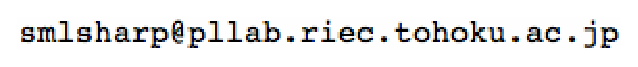
\epsfig{file=smlsharp-list.eps,width=0.4\textwidth}
共同研究の提案や各種問い合わせなどにご利用ください.
\end{itemize}
\else%%%%%%%%%%%%%%%%%%%%%%%%%%%%%%%%%%%%%%%%%%%%%%%%%%%%%%%%%%%%%%%%%%%%
	At present (March 2014), \smlsharp{} is being developed by
\begin{itemize}
\item 
Atsushi Ohori(RIEC, Tohoku University)
\item 
Katsuhiro Ueno (RIEC, Tohoku University)
\end{itemize}
with help of graduate students.

	The past \smlsharp{} development team members include (with the
affiliation at the time of development):
\begin{itemize}
\item Atsushi Ohori (School of Information Science, JAIST; RIEC, Tohoku University)
\item Kiyoshi Yamatodani (Sanpukoubou Inc)
\item Nguyen Huu Duc (School of Information Science, JAIST; RIEC, Tohoku University)
\item Liu Bochao (School of Information Science, JAIST; RIEC, Tohoku University)
\item Satoshi Osaka (School of Information Science, JAIST)
\item Katsuhiro Ueno (School of Information Science, JAIST; RIEC, Tohoku University)
\end{itemize}

	Contact information regarding \smlsharp{}:
\begin{itemize}
\item \smlsharp{} home page:
\url{http://www.pllab.riec.tohoku.ac.jp/smlsharp/ja/}

\item \smlsharp{} mailing list:
{\tt smlsharp-list@pllab.riec.tohoku.ac.jp}

	This list is for general discussion on \smlsharp{}.
	We use Japanese and English in discussion.
	To post a message, you need to subscribe to this list.
	All the messages are made available on the Web.

%%%%%%%%%%%%%%%%%%ToDo: 参加方法
%How to subscribe:\url{http://www.pllab.riec.tohoku.ac.jp/mailman/listinfo.cgi/smlsharp-list?language=ja}\\
%Mail archive:\url{http://www.pllab.riec.tohoku.ac.jp/pipermail/smlsharp-list/}

\item \smlsharp{} twitter account:
{\tt @smlsharp}

	We tweet the latest information about \smlsharp{} on this account.

\item Email address of the \smlsharp{} development team :
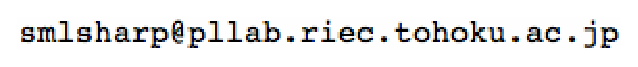
\epsfig{file=smlsharp-list.eps,width=0.4\textwidth}

Send your questions, requests and comments to the development team.
\end{itemize}
\fi%%%%<<<<<<<<<<<<<<<<<<<<<<<<<<<<<<<<<<<<<<<<<<<<<<<<<<<<<<<<<<<<<<<<<<

\section{\txt{謝辞}{Acknowledgments}}
\label{sec:acknowledgements}
	
\ifjp%>>>>>>>>>>>>>>>>>>>>>>>>>>>>>>>>>>>>>>>>>>>>>>>>>>>>>>>>>>>>>>>>>>>
	2003年にスタートした\smlsharp{}開発の過程では,以下を含む色々な
ご指導やご協力を頂きました.
	ここに謝意を表します.
\else%%%%%%%%%%%%%%%%%%%%%%%%%%%%%%%%%%%%%%%%%%%%%%%%%%%%%%%%%%%%%%%%%%%%
	From its start in 2003, we have benefited from many pepples and
ogranizations.
\fi%%%%<<<<<<<<<<<<<<<<<<<<<<<<<<<<<<<<<<<<<<<<<<<<<<<<<<<<<<<<<<<<<<<<<<
	
\subsection{\txt{プロジェクトファンディング}{Project funding}}

\ifjp%>>>>>>>>>>>>>>>>>>>>>>>>>>>>>>>>>>>>>>>>>>>>>>>>>>>>>>>>>>>>>>>>>>>
	\smlsharp{}言語の研究開発は,2003年から5年間の文部科学省リーディ
ングプロジェクトe-Society基盤ソフトウェアの総合開発「高い生産性をもつ高
信頼ソフトウェア作成技術の開発」
(\url{http://www.tkl.iis.u-tokyo.ac.jp/e-society/index.html)}
の一つの課題
「プログラムの自動解析に基づく高信頼ソフトウェアシステム構築技術」(究代
表者:大堀 淳)としてスタートをきることができました.
	このプロジェクトの主要な目標が\smlsharp{}言語コンパイラの開発で
した.
	\smlsharp{}は開発ソースの総量が\smlsharpSize{}行を超える大規模シ
ステムです.
	このプロジェクトの支援がなければ,\smlsharp{}の開発は困難であっ
たと思われます.
	文部科学省,e-Societyの領域代表の片山卓也先生,および関係各位に
深謝いたします.
\else%%%%%%%%%%%%%%%%%%%%%%%%%%%%%%%%%%%%%%%%%%%%%%%%%%%%%%%%%%%%%%%%%%%%
	\smlsharp{} development was started as a part of the 5 year
project 
``e-Society leading project: highly productive reliable software
development technologies (Project Director: Professor Takuya Katayama)'' 
under the title
``
reliable software development technology based on automatic program analysis
(chief investigator: Atsushi Ohori)
''
(\url{http://www.tkl.iis.u-tokyo.ac.jp/e-society/index.html})
sponsored by the Japan ministry of science, education and technologies.
\fi%%%%<<<<<<<<<<<<<<<<<<<<<<<<<<<<<<<<<<<<<<<<<<<<<<<<<<<<<<<<<<<<<<<<<<

\subsection{
\txt{\smlsharp{}が使用しているソフトウエア}
    {Third-party code and software tool used in \smlsharp{} development}
}

\ifjp%>>>>>>>>>>>>>>>>>>>>>>>>>>>>>>>>>>>>>>>>>>>>>>>>>>>>>>>>>>>>>>>>>>>
	\smlsharp{}言語は,第1.0版以降は,\smlsharp{}自身でコンパ
イルし開発を行なっていますが,それ以前は,Standard ML of New Jerseyおよ
びMLtonのStandard MLコンパイラを使って開発を行いました.

	\smlsharp{}は前節(\ref{sec:smlsharpTeam})の開発チー
ムによって開発されたソフトウェアです.
	ソースコードの殆どをスクラッチから開発しましたが,一部に以下のコー
ドを利用しています.

\begin{center}
\begin{tabular}{|l|l|l|}
\hline
内容 & \smlsharp{}ソース上の位置 & ソース
\\\hline
ML-Yacc & src/ml-yacc  & Standard ML of New Jersey 110.73
\\\hline
ML-Lex & src/ml-lex  & Standard ML of New Jersey 110.73
\\\hline
SML/NJ Library & src/smlnj-lib &  Standard ML of New Jersey 110.73
\\\hline
TextIO,
BinIO,
OS,
Timer
&
src/smlnj
&
Standard ML of New Jersey 110.73
\\\hline
浮動小数点/
文字列変換関数
&
src/runtime/netlib
&
the Netlib
\\\hline
SMLFormatの
SML文法定義
&
src/smlformat/generator/main/
&
Standard ML of New Jersey 110.73
\\\hline
\end{tabular}
\end{center}

	これらソースは,いずれも\smlsharp{}ライセンスと整合性あるライセ
ンスで配布されているオープンソースソフトウェアです.
	「\smlsharp{}ソース上の位置」にそれぞれのライセンスが添付されて
います.
\else%%%%%%%%%%%%%%%%%%%%%%%%%%%%%%%%%%%%%%%%%%%%%%%%%%%%%%%%%%%%%%%%%%%%

	Since version 1.0 had completed, \smlsharp{} has been
developed by the \smlsharp{} compiler itself.
	Before the \version{} version, we had used Standard ML of New
Jersey compiler for development and MLTon compiler for building
distributions.

	The \smlsharp{} compiler is a software developed by the
\smlsharp{} development team (\ref{sec:smlsharpTeam}).
	We have wrote most of the code of \smlsharp{} compiler from
scratch, except for the following code: 

\begin{center}
\begin{tabular}{|c|c|c|}
\hline
contents & location in \smlsharp{} distribution & source code
\\\hline
ML-Yacc & src/ml-yacc  & Standard ML of New Jersey 110.73
\\\hline
ML-Lex & src/ml-lex  & Standard ML of New Jersey 110.73
\\\hline
SML/NJ Library & src/smlnj-lib &  Standard ML of New Jersey 110.73
\\\hline
{\tt TextIO},
{\tt BinIO},
{\tt OS},
{\tt Timer}
structures
&
src/smlnj
&
Standard ML of New Jersey 110.73
\\\hline
floating point-string conversion
(dtoa.c)
&
src/runtime/netlib
&
the Netlib
\\\hline
SML grammar definition used 
in SMLFormat tool
&
src/smlformat/generator/main/
&
Standard ML of New Jersey 110.73
\\\hline
\end{tabular}
\end{center}

	All of the above are open-source software that are compatible
with \smlsharp{} license.
	The \smlsharp{} source distribution includes the license of each
of them at the ``location in \smlsharp{} distribution'' show above.
\fi%%%%<<<<<<<<<<<<<<<<<<<<<<<<<<<<<<<<<<<<<<<<<<<<<<<<<<<<<<<<<<<<<<<<<<

\subsection{\txt{研究開発協力者}{Collaborators}}

\ifjp%>>>>>>>>>>>>>>>>>>>>>>>>>>>>>>>>>>>>>>>>>>>>>>>>>>>>>>>>>>>>>>>>>>>
	\smlsharp{}言語の開発にあたっては,多くの人々からの指導を受けま
した.
	過去現在の開発チーム(第(\ref{sec:smlsharpTeam})節)以外で特に
貢献のあった方々は以下の通りです.
\begin{itemize}
\item 篠埜功氏.
大堀と共に,関数フュージョン機能を持つ新たしいインラインの理論および
その実験的な実装を行いました.
	この機能は実験的な実装がありますが,まだ十分な完成度が得られてお
らず\smlsharp{}\version{}版に組み込まれていませんが,将来取り入れたいと
考えています.
\item 大友聡顕氏.
	大堀,上野と共に,オブジェクトを動かさないGCの研究開発に携わり,
初期の実験的な実装を行い,この方式が有望であることを確認しました.
	この成果は,現在のオブジェクトを動かさないGCの方式の開発と実装の
契機となったものです.
\end{itemize}
	これらの方々以外にも,\smlsharp{}は,大堀等との共同で行なった様々
な型理論やコンパイル方式の基礎研究を基に設計されています.
	現在の\smlsharp{}言語に直接生かされている出版された基礎研究成果
には以下のものが含まれます.
\begin{itemize}
\item レコード多相性の理論\cite{ohor92popl,ohor95toplas}.
\item データベースの型推論\cite{ohor88lfp}.
\item データベース言語(Machiavelli)\cite{ohor89sigmod,bune96tods}.
\item ランク1多相性の型理論\cite{ohor99icfp}.
\item MLのunboxed意味論\cite{ohor97unbox}.
\item MLにおける自然なデータ表現\cite{nguyen06ppdp}.
\item オブジェクトを動かさないGC\cite{ueno11icfp}.
\item 軽量の関数融合\cite{ohor07popl}.
\end{itemize}
	それ以外にも多くの共同研究者から色々な機会に示唆や助言を頂いてお
り,それらは1989年にまで遡りますが,それらの方々の列挙は割愛させてい
ただきます.
\else%%%%%%%%%%%%%%%%%%%%%%%%%%%%%%%%%%%%%%%%%%%%%%%%%%%%%%%%%%%%%%%%%%%%

	Many people have contributed to research and development of
\smlsharp{}.
	In addition to the development team (Section
\ref{sec:smlsharpTeam}), the following people directly contributed to 
\smlsharp{} research.
\begin{itemize}
\item Isao Sasano.
With Atsushi Ohori, he investigated 
``Lightweight fusion by fixed point promotion'' and 
developed an experimental inlining module that performs lightweight
fusion.
	This feature is experimental and has not yet been integrated in
\smlsharp{} compiler, but we plan to adopt this method in a future
version.
\item Toshihiko Otomo.
	With Atsushi Ohori and Katsuhiro Ueno, he investigated the
possibility of non-moving collector and showed an initial experimental
result indicating that a non-moving GC is viable in functional
languages.
\end{itemize}
	Many other people helped us through collaborative research with
Atsushi Ohori and others to develop type-theory and compilation methods
that underlie \smlsharp{} compiler.
	\smlsharp{} compiler is directly based on the
following research results, some of them were collaboratively done.
\begin{itemize}
\item record polymorphism \cite{ohor92popl,ohor95toplas}.
\item database type inference \cite{ohor88lfp}.
\item database language (Machiavelli)\cite{ohor89sigmod,bune96tods}.
\item rank-1 polymorphism \cite{ohor99icfp}.
\item unboxed semantics of ML \cite{ohor97unbox}.
\item natural data representation for ML \cite{nguyen06ppdp}.
\item efficient non-moving GC\cite{ueno11icfp}.
\item lightweight fusion \cite{ohor07popl}.
\end{itemize}
	We have also benefited from many other researchers from 1989.
	We refrain from compiling a comprehensive list, which seems to
be impossible. 
\fi%%%%<<<<<<<<<<<<<<<<<<<<<<<<<<<<<<<<<<<<<<<<<<<<<<<<<<<<<<<<<<<<<<<<<<

\section{\txt{\smlsharp{}ライセンス}{\smlsharp{} License}}
\label{sec:smlsharpLicence}

Copyright (c) 2006 - 2014, Tohoku University.\\
All rights reserved.\\

Redistribution and use in source and binary forms, with or without
modification, are permitted provided that the following conditions are
met:

\begin{itemize}
\item 
  Redistributions of source code must retain the above copyright
  notice, this list of conditions and the following disclaimer. 
\item 
  Redistributions in binary form must reproduce the above
  copyright notice, this list of conditions and the following disclaimer
  in the documentation and/or other materials provided with the
  distribution. 
\item 
  Neither the name of Tohoku University nor the names of its
  contributors may be used to endorse or promote products derived from
  this software without specific prior written permission.  
\end{itemize}

THIS SOFTWARE IS PROVIDED BY TOHOKU UNIVERSITY AND CONTRIBUTORS "AS IS"
AND ANY EXPRESS OR IMPLIED WARRANTIES, INCLUDING, BUT NOT LIMITED TO,
THE IMPLIED WARRANTIES OF MERCHANTABILITY AND FITNESS FOR A PARTICULAR
PURPOSE ARE DISCLAIMED. IN NO EVENT SHALL TOHOKU UNIVERSITY OR
CONTRIBUTORS BE LIABLE FOR ANY DIRECT, INDIRECT, INCIDENTAL, SPECIAL,
EXEMPLARY, OR CONSEQUENTIAL DAMAGES (INCLUDING, BUT NOT LIMITED TO,
PROCUREMENT OF SUBSTITUTE GOODS OR SERVICES; LOSS OF USE, DATA, OR
PROFITS; OR BUSINESS INTERRUPTION) HOWEVER CAUSED AND ON ANY THEORY OF
LIABILITY, WHETHER IN CONTRACT, STRICT LIABILITY, OR TORT (INCLUDING
NEGLIGENCE OR OTHERWISE) ARISING IN ANY WAY OUT OF THE USE OF THIS
SOFTWARE, EVEN IF ADVISED OF THE POSSIBILITY OF SUCH DAMAGE.

\section{
\txt{\smlsharp{}第\version{}版の機能と制限}
{Limitations in \smlsharp{} version \version{}}
}
\label{sec:smlsharpLimitation}

\ifjp%>>>>>>>>>>>>>>>>>>>>>>>>>>>>>>>>>>>>>>>>>>>>>>>>>>>>>>>>>>>>>>>>>>>
	我々開発チームは第\ref{sec:whatIsSmlsharp}節でのべた機能をすべて
開発し\smlsharp{}開発開始時に目標とした機能を実現しています.
	第\version{}版にその殆どが含まれていますが,以下の制約があります.
\begin{enumerate}
\item POSIX ネイティブスレッド.
	この機能は現時点では,十分にテストされていないため,デフォルトで
はオフになっています.
	システム構築時({\tt ./configure}時)に{\tt --enable-thread}
を指定すればオンになり,コンパイラはPOSIX thread対応のコードを生成します.
	POSIX thread APIを{\tt \_import}すれば,マルチコア上でネイ
ティブスレッドが利用可能です.

\item ターゲットアーキテクチャ.
	現在の\smlsharp{}コンパイラは,32ビットのIntelアーキテクチャ
(x86, IA-32)向けのコードのみ生成可能です.
	将来,マルチターゲット化を行う予定です.
	特に,Intel系64ビットアーキテクチャ(x64またはamd64)への対応は
近い将来行う予定です.
	\smlsharp{}\version{}版はコンパイラバックエンドにLLVMを用いており,
この対応は容易と思われます.

%\item Windows版の対話型ループの制約.
%	\smlsharp{}\version{}版は,すべて一つのネイティブコードコンパイ
%ラで動いています.
%	対話型ループも,(1)ユーザ入力のコンパイル,
%(2)現在のコンパイラにリンク,
%(3)動的にロード,のサイクルによって実現されています.
%	この中で(2)のリンクをWindowsシステム上で実現するためには,シ
%ステムの制約上,これまでに作られたオブジェクトファイル毎にリンクのための
%ファイルをコマンドラインで指定する必要があります.
%	このファイル数が,対話型環境での入力に従って増えて行きます.
%	そのため,Windows上の対話型環境の連続使用は,コマンドラインの最
%大文字数によって制約されます.

\item 最適化.
	現在のバージョンには,インライニングや定数の伝播などの基本的な最
適化も十分に実装されていません.
	従って,コンパイル時間,コンパイルされたコードの実行時間もともに
十分とは言えません.
%	現在,最適化の設計開発を開始しました.
	将来の版では,他の最適化コンパイラに比肩する速度が得られると期待
しています.
\end{enumerate}
\else%%%%%%%%%%%%%%%%%%%%%%%%%%%%%%%%%%%%%%%%%%%%%%%%%%%%%%%%%%%%%%%%%%%%
	We have successfully developed all the features listed in
Section~\ref{sec:whatIsSmlsharp}, which we had initially aimed at.
	The version \version{} contains most of them, with the following 
restrictions.
\begin{enumerate}
\item {\bf POSIX Native thread support}

	This feature has not yet been well tested.
	So we set it off by default.
	To enable it, give {\tt --enable-thread} to {\tt ./configure}. 
	The compiler then generate thread-safe code.
	If you import OS thread-library through {\tt \_import}
declaration, your multithread code should run on multicore CPU.

	We have also completed development of a fully concurrent
non-moving GC.
	This has not been integrated in \version{} version.
	The GC in the \version{} version is a stop-the-world multithread
extension of the non-moving GC.
	We will replace this with a fully concurrent non-moving GC in
a future version.

\item {\bf Target Architecture.}

	The current compiler only generates x86 (or IA-32) code.
	We plan to support any other platforms, in particular amd64 (or x64),
in near future.
	Since \smlsharp{}\version{} uses LLVM as its compiler backend,
it seems to be easy for \smlsharp{} to support multiple platforms.

\item {\bf Optimization.}

	In this version, optimization is far from adequate; it does not
even implement standard ones such as inlining and constant propagation.
	So both the compilation time and the speed of generated code are
not very satisfactory.
	We have started design and development of optimizing \smlsharp{}
compiler, and hope that we will provide an optimized \smlsharp{}
compiler that is as fast as other mature compilers.

%\item {\bf Interface language.}
%
%	To support separate compilation, we have defined the interface
%language for \smlsharp{} source code.
%	This is our initial design and has a room of improvement.
%	We hope to improve the interface language based on our experience
%and other user's comments and requests.

%\item {\bf SQL integration.}
%
%	The current version only supports PostgreSQL.
%	The available SQL constructs are also limited.
%	In future version, we shall support fuller SQL syntax and
%multiple servers including MySQL.

%\item {\bf Interactive loop on Windows Systems.}
%
%	\smlsharp{} realizes interactive loop by (1) compiling the input
%to an object file, (2) linking with the currently running system to
%generate a dynamically loadable file, and then (3) dynamically loading
%the object code using {\tt dlopen}. 
%	In Windows systems, performing the linking in step 2 requires
%to specify a link information file for each of all the previous object
%files.
%	This implies that the command-line arguments to \smlsharp{}
%compiler uses in step 2 keep increasing during the interactive session,
%and will hit the limit of the command-line length. 
%	At that point, the interactive session may stall.

\end{enumerate}
\fi%%%%<<<<<<<<<<<<<<<<<<<<<<<<<<<<<<<<<<<<<<<<<<<<<<<<<<<<<<<<<<<<<<<<<<

% \section{第1章の用語解説及ぶFAQ}
% \label{sec:glossary1}
% 
% \begin{description}
% \item[BSDスタイルライセンス] 
% 二次著作物に関する制限が少ないオープンソースソフトウェアライセンスの一つ.
% 
% BSDスタイルライセンスでは,ライセンス内容をドキュメント等に表示する限り,
% ソースおよびバイナリ形式をとわず,コードの使用,変更,再配布を認めている.
% これにより,二次著作物,つまりそのソフトを利用して作成される種々の製品を,
% 自由に作成し配布や販売することができる.
% 
% 正確にな内容は英文のBSDライセンス(BSD License,Berkeley Software
% Distribution License)を参照.
% 
% 
% \item[メタ] 
% 「後に」あるいは「越えて」といった位置を表すギリシャ語.
% この接頭語を含むギリシャ語metaphsicaがアリストテレスのよって書かれた名前
% の付けられなかった本の題名の代わに使われることによって,
% 「「自然学」の後に位置する本」という意味のmetaphsicaが,
% その本の内容である「哲学,形而上学(metaphisics)」
% を意味する用語として定着した.
% それに伴い,もともとの位置の概念であったmetaに,自然学を超越する
% という意味が与えられ,種々の分野で使用されようになった.
% たとえば言語学の分野では,metaは,通常の言語の使用を分析するために用いる
% 言語として使用される.
% \end{description}
% 
% FAQ:
% \begin{itemize}
% \item 
% {[Q]} \smlsharp{}の開発に参加したいのですが?\\
% {[A]} もちろん可能です.意欲のある方はご連絡ください.一緒にプログラミング
% 言語の色々な機能を実現していきましょう.今後,研究室以外の人々とのソース
% の共有や変更の管理等の体制を整えていく予定です.
% 
% \item  
% {[Q]} 東北大学電気通信研究所でプログラミングを学ぶことができますか?\\
% {[A]} 東北大学電気通信研究所の不タッフ(教授,准教授,助教)は,学部は工学
% 部,大学院は情報科学研究科または工学研究科大学院の教員を兼務し,工学部知
% 能情報システム総合学科の学部4年生,および教員の所属する情報科学研究科お
% よび工学研究科大学院の学生を受け入れています.大堀研究室は情報科学研究科
% の教員を兼務しています.
% 
% 学部の場合は,工学部知能情報システム総合学科に,大学院なら情報科学研究科
% に入学し大堀研究室を志望すれば,我々と一緒に\smlsharp{}やその他プログラ
% ミング言語及びデータベースの研究開発を思う存分行うことができます.
% 
% \end{itemize}


\part{\txt{概要}{Overview}}
\label{part:outline}

\chapter{\txt{はじめに}{Preface}}

\ifjp%>>>>>>>>>>>>>>>>>>>>>>>>>>>>>>>>>>>>>>>>>>>>>>>>>>>>>>>>>>>>>>>>>>>
	本書は東北大学電気通信研究所で開発された関数型プログラミング言語
\smlsharp{}の公式ドキュメントです.
	\smlsharp{}の概要,プログラミングチュートリアル,参照マニュアル,
ツールなどの情報を含む総合ドキュメントを意図しています.
	関数型言語に慣れた人はもちろん,これからプログラミングを始めようと
する人にも,\smlsharp{}言語を使って高度なプログラミングを書き始めるために
十分な情報を提供します.
	特に,第\ref{part:tutorial}部のチュートリアルは,関数型言語の基
本的な考え方やMLプログラミングの基礎を含んでおり,ML言語の手軽な教科書と
しても使用できます.
	ML言語をより本格的に学ぶには,Standard MLの教科書
\cite{ohori00sml}をご参照ください.
  
	\smlsharp{}は,これら教科書で書かれたStandard MLと後方互換性のあ
る言語です.
	ネイティブコードコンパイラですが,対話型プログラミングもサポート
しており,だれでも手軽にMLプログラミングを楽しむことができます.
	さらに,\smlsharp{}が実現しているC言語とのシームレスな連携などの
機能は,高度で信頼性の要求される本格的な実用的システムの開発にも威力を
発揮すると信じています. 
  
	本ドキュメントを参考に,\smlsharp{}プログラミングをお楽しみくだ
さい. 
	不明な点や要望等は著者にご連絡ください.

\else%%%%%%%%%%%%%%%%%%%%%%%%%%%%%%%%%%%%%%%%%%%%%%%%%%%%%%%%%%%%%%%%%%%%
	This is the official document of \smlsharp{}, a programming
language developed at Research Institute of Electrical Communication,
Tohoku University.
	This document intends to provide comprehensive information on
\smlsharp{}, covering a user's guide, tutorials on ML and \smlsharp{}
programming, and a reference manual.
	This \version{} version only contains an overview of \smlsharp{}
and tutorials on ML and \smlsharp{} programming, which would be
sufficient for beginners who want to start writing ML programs and
for experienced ML programmer who would like to try out or switch to
\smlsharp{}.

	Send comments and questions to the authors.

\bigskip
\bigskip

We are currently preparing the following:
\begin{itemize}
\item Part III Reference Manual
\item Part IV Programming Tools
\item Part V  Internls and Data Structures of \smlsharp{}
\end{itemize}
\fi%%%%<<<<<<<<<<<<<<<<<<<<<<<<<<<<<<<<<<<<<<<<<<<<<<<<<<<<<<<<<<<<<<<<<<

\begin{flushright}
\txt{
2016年3月\\
\authors
}
{
March, 2016\\
\authors
}
\end{flushright}

\chapter{\txt{本書の使い方}{How to read this document}}

\ifjp%>>>>>>>>>>>>>>>>>>>>>>>>>>>>>>>>>>>>>>>>>>>>>>>>>>>>>>>>>>>>>>>>>>>
    この文書の第\ref{part:outline}部の概要と第\ref{part:tutorial}部のチュー
トリアルはMLプログラミングの基礎から\smlsharp{}が提供する高度の機能まで
を習得できる構造になっています.
	先頭から順に一気にお読みになることをおすすめします.
	お急ぎの方は,以下のページにお探しの情報があるかもしれません.
\begin{itemize}
\item {\bf \smlsharp{}の名前について:}
第\ref{sec:smlsharpHistory}節.
\item {\bf インストール方法:}
第\ref{sec:tutorialInstall}節.
\item {\bf {\tt smlsgarp}コマンドの起動モードと起動パラメタ:}
第\ref{sec:tutorialSmlsharpParameter}節.
\item {\bf \smlsharp{}開発チームと連絡先情報:} 第\ref{sec:smlsharpTeam}節.
\item {\bf \smlsharp{}ホームページ:}
\url{http://www.pllab.riec.tohoku.ac.jp/smlsharp/ja/}
\item {\bf \smlsharp{} Documnet in English:}
% \url{http://www.pllab.riec.tohoku.ac.jp/smlsharp/docs/2.0/en/manual.xhtml}
\documentUrlEn
\end{itemize}   

本書に関して,以下の点をご了承ください.
\begin{itemize}
\item 随時頻繁に修正を行います.
	そのため,本文書の配布は当面xhtml形式のみとします.
	近い将来,より完成した版のPDFでの配布を検討中です.
\item
	修正・執筆にあたっては,twitterなどでの\smlsharp{}や本書へのコメントな
ども,本書の改善の参考にさせて頂いております.
	個々に言及いたしませんが,本書をご覧頂きコメントをお寄せ頂いた
方々に感謝いたします. 

\item この文書は,LaTeXとLaTeXMLを用いて作成しています.
FirefoxなどのMathMLのレンダリングが可能なブラウザでご覧ください.

\item LaTeXMLは日本語化がなされていないようです.
	本文書は{\tt jbook}クラスで書いていますが,LateXMLのpackageに
jbook用が用意されていないため,{\tt book.cls.ltxml}を
{\tt jbook.cls.ltxml}にコピーし使用しています.
	(LateXMLの日本語クラスパッケージをご存知の方はお教えください.)
\end{itemize}
\else%%%%%%%%%%%%%%%%%%%%%%%%%%%%%%%%%%%%%%%%%%%%%%%%%%%%%%%%%%%%%%%%%%%%

	The tutorials in parts~\ref{part:outline} and
\ref{part:tutorial} are structured in such a way that the reader can
learn from ML programming basics to advanced programming features
provided by \smlsharp{}.
	We recommend to read through these parts quickly in the order
they are presented.

	If you are in a harry, you may find the desired information in
one of the following pages.
\begin{itemize}
\item {\bf How to install \smlsharp{}}: Section \ref{sec:tutorialInstall}.
\item {\bf {\tt smlsharp} command parameters}: Section \ref{sec:tutorialSmlsharpParameter}.
\item {\bf \smlsharp{} development team and contact information}: 
Section \ref{sec:smlsharpTeam}.
\item {\bf On the name of \smlsharp{}}: Section \ref{sec:smlsharpHistory} (History of \smlsharp).
\item {\bf \smlsharp{} web page}: 
\url{http://www.pllab.riec.tohoku.ac.jp/smlsharp/}
\item {\bf \smlsharp{} Documnet in Japanese (プログラミング言語\smlsharp{}解説)}:
% \url{http://www.pllab.riec.tohoku.ac.jp/smlsharp/docs/2.0/ja/manual.xhtml}
\documentUrlJa
\end{itemize}

In reading this document, please note the following.
\begin{itemize}
\item 
	This \version{} version is an incomplete draft; it does not
contain the reference manual and the ML programming tutorial is
incomplete.

\item 
	This document is frequently revised and updated.
	For this reason, the currently version is distributed only on
this web server.
	In near future, we plan to include a more complete version of
this document (both in PDF and XHTML format) in the \smlsharp{}
distribution.

\item
	We appreciate those who give us comments on \smlsharp{} and
this document through some communication tools including Twitter.
	We have reflect all of them to the latest version of this
document.

\item 
	This document is written in LaTeX and processed with LaTeXML.
	It is best viewed with a MathML-capable browser such as {\bf Firefox}.
\end{itemize}
\fi%%%%<<<<<<<<<<<<<<<<<<<<<<<<<<<<<<<<<<<<<<<<<<<<<<<<<<<<<<<<<<<<<<<<<<

\chapter{\txt{本書の構成と執筆状況}{The structure and status of this document}}

	本書は以下の部から成ります.
	必要に応じて,各部をご参照ください.
\begin{enumerate}
\item
	第\ref{part:outline}部: \smlsharp{}および本書の概要を述べます.
\item
	第\ref{part:tutorial}部:
\smlsharp{}でプログラミングを始めるためのチュートリアルです.
	\smlsharp{}のインストール方法,
\smlsharp{}の初歩的な使い方,
および
レコード多相性やCとの直接連携などの\smlsharp{}の拡張機能の
概要を,豊富な例と共に説明しています.
	また,関数型言語初学者に向けた,
MLプログラミングのための環境のセットアップ方法や,
Standard MLの基本機能を用いたMLプログラミングの基本も,
本章に含まれています.
	初心者から上級者までを含む全ての\smlsharp{}ユーザーにとって,
この部の内容は有益なはずです.
\item
	第\ref{part:referenceManual}部:
Standard MLの基本機能を含む,\smlsharp{}の全ての機能を網羅した参照マニュアル
です.
\item
	第\ref{part:tools}部:
\smlsharp{}付属のツール群({\tt smllex}, {\tt smlyacc}, {\tt smlformat}など)
に関するマニュアルです.
\item
	第\ref{part:internals}部:
\smlsharp{}コンパイラの開発や関数型言語のコンパイラの構築方法に興味の
ある方を対象に,
\smlsharp{}コンパイラの内部構造を詳述します.
\item
	第\ref{part:bib}部: 参考文献のリストです.
\end{enumerate}

	現状(2016年3月),第\ref{part:referenceManual}部以降は
未完成であり,現在執筆中です.
%	従って第\ref{part:referenceManual}部以降は,あくまで参考資料と
%してご利用ください.
	各部の現在の執筆状況は以下の通りです.
\begin{enumerate}
\item
	第\ref{part:outline}部: 執筆完了
\item
	第\ref{part:tutorial}部: 執筆完了
\item
	第\ref{part:referenceManual}部: 執筆中であり,
\smlsharp{}の全機能を正確に網羅していません.
	あくまで,参考資料としてご利用ください.
	正式な参照マニュアルは,近日中に公開の予定です.
\item
	第\ref{part:tools}部: 未着手.執筆計画中です.
\item
	第\ref{part:internals}部: 未着手.執筆計画中です.
\item
	第\ref{part:bib}部: 他の部の執筆状況に応じて随時更新されます.
\end{enumerate}

%\chapter{\txt{\smlsharp{}使用上の注意}{Important notes on \smlsharp{}}}
%
%\ifjp%>>>>>>>>>>>>>>>>>>>>>>>>>>>>>>>>>>>>>>>>>>>>>>>>>>>>>>>>>>>>>>>>>>>
%
%\smlsharp{}\version{}版を使用する上で注意すべき点を列挙します.
%
%\else%%%%%%%%%%%%%%%%%%%%%%%%%%%%%%%%%%%%%%%%%%%%%%%%%%%%%%%%%%%%%%%%%%%%
%Here, we list the issues you should aware of in using \smlsharp{}
%version~\version{}.
%
%\fi%%%%<<<<<<<<<<<<<<<<<<<<<<<<<<<<<<<<<<<<<<<<<<<<<<<<<<<<<<<<<<<<<<<<<<

\chapter{\txt{\smlsharp{}の概要}{Overview of \smlsharp{}}}
\label{chap:intro}

\ifjp%>>>>>>>>>>>>>>>>>>>>>>>>>>>>>>>>>>>>>>>>>>>>>>>>>>>>>>>>>>>>>>>>>>>
本章では\smlsharp{}言語の概要を説明します.
\else%%%%%%%%%%%%%%%%%%%%%%%%%%%%%%%%%%%%%%%%%%%%%%%%%%%%%%%%%%%%%%%%%%%%
This chapter outlines the \smlsharp{} language and the compiler.
\fi%%%%<<<<<<<<<<<<<<<<<<<<<<<<<<<<<<<<<<<<<<<<<<<<<<<<<<<<<<<<<<<<<<<<<<

\section{\txt{\smlsharp{}とは?}{What is \smlsharp{}?}}
\label{sec:whatIsSmlsharp}
\ifjp%>>>>>>>>>>>>>>>>>>>>>>>>>>>>>>>>>>>>>>>>>>>>>>>>>>>>>>>>>>>>>>>>>>>

\smlsharp{}は,以下のような特徴をもったML系関数型プログラミング言語です.
\begin{enumerate}
\item {\bf Standard MLとの後方互換性.}
	\smlsharp{}は,ML系言語の標準の厳密な仕様であるStandard MLとの
後方互換性を持っています.
	Standard MLの形式的な仕様\cite{sml}を満たすすべての
プログラムをコンパイルできます.

\item {\bf レコード多相性.}
	レコード多相性\cite{ohor95toplas}は,オブジェクトやデータベース
のタプルなどに現れるラベル付きレコードをML言語に完全に統合するために必要
な型システムの機能です.
	\smlsharp{}は,この機能を完全にサポートしています.

\item {\bf SQLのシームレスな統合.}
	SQLはデータベースの標準問い合わせ言語であり,データベースを利用
するプログラムで必ず必要となる機能です.
	\smlsharp{}は,SQLの一部の機能をライブラリとして提供するのでは
なく,SQLクエリそのものを多相型をもつ第一級の式として統合しています.
	この機能により,複雑なプログラムデータベース操作を,MLプログラム
の中で直接プログラムすることができます.
	
\item {\bf C言語との直接連携.}
	システムプログラミングを含む種々のOSの機能の利用にはC言語で記述
されたライブラリへのアクセスが必要となります.
	\smlsharp{}では,名前を外部名宣言するだけで,C言語で書かれCコン
パイラでコンパイルされた関数を呼び出すことができます.

\item {\bf マルチコアCPU上のネイティブスレッドのサポート.}
	\smlsharp{}の並行かつオブジェクトを動かさないGCの機能により,
C言語との連携機能を使い,OSのスレッドライブラリを直接呼び出すことができ
ます.
	従って,OSがマルチコアCPU上での並列実行をサポートしさえすれば,
スレッドを使った高水準なMLプログラムを書き,マルチコアCPU上で効率良く
実行することができます.

\item {\bf 分割コンパイルとリンク.}
	\smlsharp{}は,従来のインクリメンタルなコンパイルではない,真の分
割コンパイルを実現しています.
	各モジュールのインターフェイスの確定後は,各モジュールを独立に開
発しコンパイルやテストできます.
	さらに,\smlsharp{}コンパイラは,分割コンパイルの対象となる各ソー
スコードを,システム標準のオブジェクトファイル(例えばLinuxならば
ELFフォーマット)にコンパイルし,システムのリンカーでCのライブラリなどと
ともにリンクします.
	この機能により,Standard MLだけでなくC言語やSQLなどをも使う
大規模プログラムを安全かつ効率的に開発することができます.

\end{enumerate}

	\smlsharp{}コンパイラおよび実行時処理系は,東北大学電気通信研究
所大堀研究室で開発され,東北大学が著作権保有するオープンソースソフトウェ
アです.
	BSDスタイルの\smlsharp{}ライセンス(\ref{sec:smlsharpLicence}節参照)に
よって公開されており,だれでも自由に利用することができます.
	このライセンスは,二次著作物(つまりコンパイラで作成されたシステ
ムなど)に関する制限の少ないフリーソフトウェアライセンスであり,企業の商
品開発にも安心して使用できます.

\else%%%%%%%%%%%%%%%%%%%%%%%%%%%%%%%%%%%%%%%%%%%%%%%%%%%%%%%%%%%%%%%%%%%%
	\smlsharp{} is a new programming language in the ML-family,
having the following features.
\begin{enumerate}
\item {\bf Downward compatibility with Standard ML.}
	\smlsharp{} can compile all programs that conform to the
definition of the Standard ML\cite{sml}.

\item {\bf Record polymorphism.}
	\smlsharp{} supports record polymorphism \cite{ohor95toplas}.
	In \smlsharp{} , field selection operators {\bf\tt \#\nonterm{label}}
and record patterns {\bf\tt \{\nonterm{field-pat},...\}} are fully
polymorphic.
	This feature is essential in modular development of programs
manipulating records, and is the key to extend ML with SQL.

\item {\bf Seamless integration of SQL.}
	\smlsharp{} seamlessly integrates (currently a subset of) SQL.
	Instead of providing built-in primitives to access
database servers, \smlsharp{} integrate SQL expressions themselves as
polymorphically-typed first-class citizens.
	This allows the programmer to directly access databases in
your polymorphic ML code.

\item {\bf Direct interface to C.}
	\smlsharp{} programs can directly call C functions of your own
coding or in system libraries.
	The programmer need only declare their names and types, without
writing mysterious ``stubs'' or conversion functions. 
	The \smlsharp{} generates external references to C functions,
which are resolved and linked by the system linker.
	Both static and dynamic linking are supported.

\item {\bf Separate compilation and linking.}
	\smlsharp{} supports true separate compilation and linking.
	By writing an interface file, each source file is compiled
separately into an object file in the standard system format (e.g.\ ELF
format.)
	The separately compiled object files are then linked together
possibly with C functions and libraries into an executable program.

\item {\bf Multithread support for multicore CPUs.}
	The non-moving GC \cite{ueno11icfp} and direct C interface allow
\smlsharp{} code to directly call POSIX thread library.
	As far as the OS thread library support a multicore CPU,
\smlsharp{} program automatically obtains multithread capability for
multicore CPUs.
	With the non-moving fully concurrent GC we have just developed, 
concurrent threads run efficiently on a multicore CPU.

\end{enumerate}

	The \smlsharp{} compiler and its runtime system are developed at
Research Institute of Electrical Communication,  Tohoku University.
	They are open-source software distributed with a BSD-style
\smlsharp{} license (\ref{sec:smlsharpLicence}).
\fi%%%%<<<<<<<<<<<<<<<<<<<<<<<<<<<<<<<<<<<<<<<<<<<<<<<<<<<<<<<<<<<<<<<<<<

\section{\txt{\smlsharp{}の歴史}{History of \smlsharp{}}}
\label{sec:smlsharpHistory}

\ifjp%>>>>>>>>>>>>>>>>>>>>>>>>>>>>>>>>>>>>>>>>>>>>>>>>>>>>>>>>>>>>>>>>>>>
	1993年,沖電気工業(株)関西総合研究所にて,大堀により,Standard
ML of New Jerseyコンパイラに多相型レコード演算を加え拡張したプロトタイプ
{\bf SML\# of Kansai}が開発されました.
	その時の\smlsharp{}のtypesメーリングリストへのアナウンスは,今で
もインターネット上に記録されています
(
\url{http://www.funet.fi/pub/languages/ml/sml%23/description}
).

	{\bf SML\# of Kansai}の名前は,このコンパイラにて初めて多相型が与えら
れたレコード演算子"{\bf \code{\#}}"を象徴するものです.
	このコンパイラは,1996年ACM TOPLASに出版されたコード多相性に関する論文
\cite{ohor95toplas}で,{\bf \smlsharp{}}の名前で紹介されています.

	その後,より完全な\smlsharp{}コンパイラの開発の努力が継続されま
した.

	2003年に,北陸先端科学技術大学院大学にて,文部科学省リーディング
プロジェクトe-Society基盤ソフトウェアの総合開発「高い生産性をもつ高信頼
ソフトウエア作成技術の開発」
(領域代表者:片山卓也)
の一つの課題
「プログラムの自動解析に基づく高信頼ソフトウェアシステム構築技術」(2003年―2008年,究代表者:大堀 淳)
(
\url{http://www.tkl.iis.u-tokyo.ac.jp/e-society/index.html}
)
として,
次世代ML系関数型言語\smlsharp{}をスクラッチから開発するプロジェクトを開始しました.

2006年4月,プロジェクトは,大堀とともに東北大学電気通信研究所に移り開発
を継続しています.

2008年のe-Societyプロジェクト終了後も,東北大学電気通信研究所大堀研究室
にて,\smlsharp{}の研究開発を続けています.

\else%%%%%%%%%%%%%%%%%%%%%%%%%%%%%%%%%%%%%%%%%%%%%%%%%%%%%%%%%%%%%%%%%%%%

	In 1993, Atsushi Ohori extended the Standard ML of New Jersey
compiler at Kansai Laboratory of Oki Electric, and named the
experimental prototype SML\# of Kansai.
	The Internet still remembers my old posting of \smlsharp{} to
the types mailing list 
(\url{http://www.funet.fi/pub/languages/ml/sml%23/description}).

	The name SML\# of Kansai symbolizes the field selector {\bf\tt
\#\nonterm{label}}, which was given a polymorphic type for the first
time by this compiler.
	This compiler was reported in the ACM TOPLAS article on record
polymorphism \cite{ohor95toplas} as {\bf \smlsharp{}}.

	To support not only record polymorphism but also
interoperability and other practically important features, we decided 
to develop a new SML-style language from scratch, and in 2003, we
started the \smlsharp{} compiler project at Japan Advanced Institute of 
Science and Technology as a part of the e-Society project 
(
\url{http://www.tkl.iis.u-tokyo.ac.jp/e-society/index.html}
).
funded by the Japan ministry of science, education and technologies

	In 2006, the project moved to Tohoku University.
\fi%%%%<<<<<<<<<<<<<<<<<<<<<<<<<<<<<<<<<<<<<<<<<<<<<<<<<<<<<<<<<<<<<<<<<<

\section{
\txt{\smlsharp{}開発チームと連絡先情報}
{\smlsharp{} Development Team and Contact Information}
}
\label{sec:smlsharpTeam}

\ifjp%>>>>>>>>>>>>>>>>>>>>>>>>>>>>>>>>>>>>>>>>>>>>>>>>>>>>>>>>>>>>>>>>>>>
	現在(2016年3月)\smlsharp{}は,
\begin{itemize}
\item 
大堀 淳(東北大学電気通信研究所)
\item 
上野雄大(東北大学電気通信研究所)
\end{itemize}
の2名が,大学院大学院情報科学研究科の大堀研究室に所属の大学院生の協力の
下,開発を行なっています.

	\smlsharp{}のこれまでの主な開発者は以下の通りです.
	(敬称は略させていただいています.
	所属は\smlsharp{}の開発に携わった時のものです.)
\begin{itemize}
\item 大堀 淳(北陸先端科学技術大学院大学情報科学研究科,東北大学電気通信研究所)
\item 大和谷 潔(算譜工房)
\item Nguyen Huu Duc(北陸先端科学技術大学院大学情報科学研究科,東北大学電気通信研究所)
\item Liu Bochao(北陸先端科学技術大学院大学情報科学研究科,東北大学電気通信研究所)
\item 纓坂 智(北陸先端科学技術大学院大学情報科学研究科)
\item 上野雄大(北陸先端科学技術大学院大学情報科学研究科,東北大学電気通信研究所)
\end{itemize}

	東北大学電気通信研究所では,\smlsharp{}に関する情報共有の目的で
以下のwebサイトやメーリングリストを管理しています.
\begin{itemize}
\item \smlsharp{}ホームページ.
\url{http://www.pllab.riec.tohoku.ac.jp/smlsharp/ja/}
コンパイラや本書を含む文書の最新版などもここからダウンロードできます.

%\item \smlsharp{}メーリングリスト
%{\tt smlsharp@ml.riec.tohoku.ac.jp}.
%\smlsharp{}に関する一般的な議論や情報交換のためのメーリングリストです.
%使用言語は日本語または英語です.投稿は購読者のみ行うことができ,投稿され
%た全てのメールはWeb上に公開されます.\\
%%%%%%%%%%%%%%%%%%%ToDo: 参加方法
%%参加方法:\url{http://www.pllab.riec.tohoku.ac.jp/mailman/listinfo.cgi/smlsharp-list?language=ja}\\
%%アーカイブ:\url{http://www.pllab.riec.tohoku.ac.jp/pipermail/smlsharp-list/}

\item Twitterアカウント {\tt @smlsharp}.
\smlsharp{}に関する最新情報をツイートします.

%\item \smlsharp{}開発者への連絡メールアドレス.
%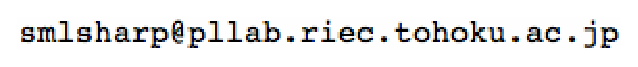
\epsfig{file=smlsharp-list.eps,width=0.4\textwidth}
%共同研究の提案や各種問い合わせなどにご利用ください.

\item \smlsharp{}開発者への連絡メールアドレス
{\tt smlsharp-dev@ml.riec.tohoku.ac.jp}.
%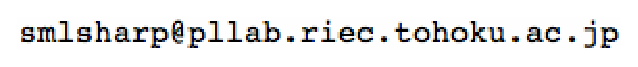
\epsfig{file=smlsharp-list.eps,width=0.4\textwidth}
各種問い合わせや共同研究の提案などにご利用ください.

\end{itemize}
\else%%%%%%%%%%%%%%%%%%%%%%%%%%%%%%%%%%%%%%%%%%%%%%%%%%%%%%%%%%%%%%%%%%%%
	At present (March 2016), \smlsharp{} is being developed by
\begin{itemize}
\item 
Atsushi Ohori(RIEC, Tohoku University)
\item 
Katsuhiro Ueno (RIEC, Tohoku University)
\end{itemize}
with help of graduate students.

	The past \smlsharp{} development team members include (with the
affiliation at the time of development):
\begin{itemize}
\item Atsushi Ohori (School of Information Science, JAIST; RIEC, Tohoku University)
\item Kiyoshi Yamatodani (Sanpukoubou Inc)
\item Nguyen Huu Duc (School of Information Science, JAIST; RIEC, Tohoku University)
\item Liu Bochao (School of Information Science, JAIST; RIEC, Tohoku University)
\item Satoshi Osaka (School of Information Science, JAIST)
\item Katsuhiro Ueno (School of Information Science, JAIST; RIEC, Tohoku University)
\end{itemize}

	Contact information regarding \smlsharp{}:
\begin{itemize}
\item \smlsharp{} home page:
\url{http://www.pllab.riec.tohoku.ac.jp/smlsharp/ja/}

%\item \smlsharp{} mailing list:
%{\tt smlsharp-list@pllab.riec.tohoku.ac.jp}
%
%	This list is for general discussion on \smlsharp{}.
%	We use Japanese and English in discussion.
%	To post a message, you need to subscribe to this list.
%	All the messages are made available on the Web.

%%%%%%%%%%%%%%%%%%ToDo: 参加方法
%How to subscribe:\url{http://www.pllab.riec.tohoku.ac.jp/mailman/listinfo.cgi/smlsharp-list?language=ja}\\
%Mail archive:\url{http://www.pllab.riec.tohoku.ac.jp/pipermail/smlsharp-list/}

\item \smlsharp{} twitter account:
{\tt @smlsharp}

	We tweet the latest information about \smlsharp{} on this account.

\item Email address of the \smlsharp{} development team :
{\tt smlsharp-dev@ml.riec.tohoku.ac.jp}
%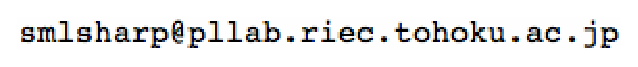
\epsfig{file=smlsharp-list.eps,width=0.4\textwidth}

Send your questions, requests, and comments to the development team.
\end{itemize}
\fi%%%%<<<<<<<<<<<<<<<<<<<<<<<<<<<<<<<<<<<<<<<<<<<<<<<<<<<<<<<<<<<<<<<<<<

\section{\txt{謝辞}{Acknowledgments}}
\label{sec:acknowledgements}
	
\ifjp%>>>>>>>>>>>>>>>>>>>>>>>>>>>>>>>>>>>>>>>>>>>>>>>>>>>>>>>>>>>>>>>>>>>
	2003年にスタートした\smlsharp{}開発の過程では,以下を含む色々な
ご指導やご協力を頂きました.
	ここに謝意を表します.
\else%%%%%%%%%%%%%%%%%%%%%%%%%%%%%%%%%%%%%%%%%%%%%%%%%%%%%%%%%%%%%%%%%%%%
	From its start in 2003, we have benefited from many pepples and
ogranizations.
\fi%%%%<<<<<<<<<<<<<<<<<<<<<<<<<<<<<<<<<<<<<<<<<<<<<<<<<<<<<<<<<<<<<<<<<<
	
\subsection{\txt{プロジェクトファンディング}{Project funding}}

\ifjp%>>>>>>>>>>>>>>>>>>>>>>>>>>>>>>>>>>>>>>>>>>>>>>>>>>>>>>>>>>>>>>>>>>>
	\smlsharp{}言語の研究開発は,2003年から5年間の文部科学省リーディ
ングプロジェクトe-Society基盤ソフトウェアの総合開発「高い生産性をもつ高
信頼ソフトウェア作成技術の開発」
(\url{http://www.tkl.iis.u-tokyo.ac.jp/e-society/index.html)}
の一つの課題
「プログラムの自動解析に基づく高信頼ソフトウェアシステム構築技術」(究代
表者:大堀 淳)としてスタートをきることができました.
	このプロジェクトの主要な目標が\smlsharp{}言語コンパイラの開発で
した.
	\smlsharp{}は開発ソースの総量が\smlsharpSize{}行を超える大規模シ
ステムです.
	このプロジェクトの支援がなければ,\smlsharp{}の開発は困難であっ
たと思われます.
	文部科学省,e-Societyの領域代表の片山卓也先生,および関係各位に
深謝いたします.
\else%%%%%%%%%%%%%%%%%%%%%%%%%%%%%%%%%%%%%%%%%%%%%%%%%%%%%%%%%%%%%%%%%%%%
	\smlsharp{} development was started as a part of the 5 year
project 
``e-Society leading project: highly productive reliable software
development technologies (Project Director: Professor Takuya Katayama)'' 
under the title
``
reliable software development technology based on automatic program analysis
(chief investigator: Atsushi Ohori)
''
(\url{http://www.tkl.iis.u-tokyo.ac.jp/e-society/index.html})
sponsored by the Japan ministry of science, education and technologies.
\fi%%%%<<<<<<<<<<<<<<<<<<<<<<<<<<<<<<<<<<<<<<<<<<<<<<<<<<<<<<<<<<<<<<<<<<

\subsection{
\txt{\smlsharp{}が使用しているソフトウエア}
    {Third-party code and software tool used in \smlsharp{} development}
}

\ifjp%>>>>>>>>>>>>>>>>>>>>>>>>>>>>>>>>>>>>>>>>>>>>>>>>>>>>>>>>>>>>>>>>>>>
	\smlsharp{}言語は,第1.0版以降は,\smlsharp{}自身でコンパ
イルし開発を行なっていますが,それ以前は,Standard ML of New Jerseyおよ
びMLtonのStandard MLコンパイラを使って開発を行いました.

	\smlsharp{}は前節(\ref{sec:smlsharpTeam})の開発チー
ムによって開発されたソフトウェアです.
	ソースコードの殆どをスクラッチから開発しましたが,一部に以下のコー
ドを利用しています.

\begin{center}
\begin{tabular}{|l|l|l|}
\hline
内容 & \smlsharp{}ソース上の位置 & ソース
\\\hline
ML-Yacc & src/ml-yacc  & Standard ML of New Jersey 110.73
\\\hline
ML-Lex & src/ml-lex  & Standard ML of New Jersey 110.73
\\\hline
SML/NJ Library & src/smlnj-lib &  Standard ML of New Jersey 110.73
\\\hline
TextIO,
BinIO,
OS,
Date,
Timer
&
src/smlnj
&
Standard ML of New Jersey 110.73
\\\hline
浮動小数点/
文字列変換関数
&
src/runtime/netlib
&
the Netlib
\\\hline
SMLFormatの
SML文法定義
&
src/smlformat/generator/main/
&
Standard ML of New Jersey 110.73
\\\hline
\end{tabular}
\end{center}

	これらソースは,いずれも\smlsharp{}ライセンスと整合性あるライセ
ンスで配布されているオープンソースソフトウェアです.
	「\smlsharp{}ソース上の位置」およびソースパッケージのトップレベル
にそれぞれのライセンスが添付されています.
\else%%%%%%%%%%%%%%%%%%%%%%%%%%%%%%%%%%%%%%%%%%%%%%%%%%%%%%%%%%%%%%%%%%%%

	Since version 1.0 had completed, \smlsharp{} has been
developed by the \smlsharp{} compiler itself.
	Before the \version{} version, we had used Standard ML of New
Jersey compiler for development and MLTon compiler for building
distributions.

	The \smlsharp{} compiler is a software developed by the
\smlsharp{} development team (\ref{sec:smlsharpTeam}).
	We have wrote most of the code of \smlsharp{} compiler from
scratch, except for the following code: 

\begin{center}
\begin{tabular}{|c|c|c|}
\hline
contents & location in \smlsharp{} distribution & source code
\\\hline
ML-Yacc & src/ml-yacc  & Standard ML of New Jersey 110.73
\\\hline
ML-Lex & src/ml-lex  & Standard ML of New Jersey 110.73
\\\hline
SML/NJ Library & src/smlnj-lib &  Standard ML of New Jersey 110.73
\\\hline
{\tt TextIO},
{\tt BinIO},
{\tt OS},
{\tt Date},
{\tt Timer}
structures
&
src/smlnj
&
Standard ML of New Jersey 110.73
\\\hline
floating point-string conversion
(dtoa.c)
&
src/runtime/netlib
&
the Netlib
\\\hline
SML grammar definition used 
in SMLFormat tool
&
src/smlformat/generator/main/
&
Standard ML of New Jersey 110.73
\\\hline
\end{tabular}
\end{center}

	All of the above are open-source software that are compatible
with \smlsharp{} license.
	The \smlsharp{} source distribution includes the license of each
of them at the ``location in \smlsharp{} distribution'' show above.
\fi%%%%<<<<<<<<<<<<<<<<<<<<<<<<<<<<<<<<<<<<<<<<<<<<<<<<<<<<<<<<<<<<<<<<<<

\subsection{\txt{研究開発協力者}{Collaborators}}

\ifjp%>>>>>>>>>>>>>>>>>>>>>>>>>>>>>>>>>>>>>>>>>>>>>>>>>>>>>>>>>>>>>>>>>>>
	\smlsharp{}言語の開発にあたっては,多くの人々からの指導を受けま
した.
	過去現在の開発チーム(第(\ref{sec:smlsharpTeam})節)以外で特に
貢献のあった方々は以下の通りです.
\begin{itemize}
\item 篠埜功氏.
	大堀と共に,関数フュージョン機能を持つ新たしいインラインの理論お
よびその実験的な実装を行いました.
	この機能は実験的な実装がありますが,まだ十分な完成度が得られてお
らず\smlsharp{}\version{}版に組み込まれていませんが,将来取り入れたいと
考えています.
\item 大友聡顕氏.
	大堀,上野と共に,オブジェクトを動かさないGCの研究開発に携わり,
初期の実験的な実装を行い,この方式が有望であることを確認しました.
	この成果は,現在のオブジェクトを動かさないGCの方式の開発と実装の
契機となったものです.
\end{itemize}
	これらの方々以外にも,\smlsharp{}は,大堀等との共同で行なった様々
な型理論やコンパイル方式の基礎研究を基に設計されています.
	現在の\smlsharp{}言語に直接生かされている出版された基礎研究成果
には以下のものが含まれます.
\begin{itemize}
\item レコード多相性の理論\cite{ohor92popl,ohor95toplas}.
\item データベースの型推論\cite{ohor88lfp}.
\item データベース言語(Machiavelli)\cite{ohor89sigmod,bune96tods}.
\item ランク1多相性の型理論\cite{ohor99icfp}.
\item MLのunboxed意味論\cite{ohor97unbox}.
\item MLにおける自然なデータ表現\cite{nguyen06ppdp}.
\item オブジェクトを動かさないGC\cite{ueno11icfp}.
\item 軽量の関数融合\cite{ohor07popl}.
\end{itemize}
	それ以外にも多くの共同研究者から色々な機会に示唆や助言を頂いてお
り,それらは1989年にまで遡りますが,それらの方々の列挙は割愛させてい
ただきます.
\else%%%%%%%%%%%%%%%%%%%%%%%%%%%%%%%%%%%%%%%%%%%%%%%%%%%%%%%%%%%%%%%%%%%%

	Many people have contributed to research and development of
\smlsharp{}.
	In addition to the development team (Section
\ref{sec:smlsharpTeam}), the following people directly contributed to 
\smlsharp{} research.
\begin{itemize}
\item Isao Sasano.
With Atsushi Ohori, he investigated 
``Lightweight fusion by fixed point promotion'' and 
developed an experimental inlining module that performs lightweight
fusion.
	This feature is experimental and has not yet been integrated in
\smlsharp{} compiler, but we plan to adopt this method in a future
version.
\item Toshihiko Otomo.
	With Atsushi Ohori and Katsuhiro Ueno, he investigated the
possibility of non-moving collector and showed an initial experimental
result indicating that a non-moving GC is viable in functional
languages.
\end{itemize}
	Many other people helped us through collaborative research with
Atsushi Ohori and others to develop type-theory and compilation methods
that underlie \smlsharp{} compiler.
	\smlsharp{} compiler is directly based on the
following research results, some of them were collaboratively done.
\begin{itemize}
\item record polymorphism \cite{ohor92popl,ohor95toplas}.
\item database type inference \cite{ohor88lfp}.
\item database language (Machiavelli)\cite{ohor89sigmod,bune96tods}.
\item rank-1 polymorphism \cite{ohor99icfp}.
\item unboxed semantics of ML \cite{ohor97unbox}.
\item natural data representation for ML \cite{nguyen06ppdp}.
\item efficient non-moving GC\cite{ueno11icfp}.
\item lightweight fusion \cite{ohor07popl}.
\end{itemize}
	We have also benefited from many other researchers from 1989.
	We refrain from compiling a comprehensive list, which seems to
be impossible. 
\fi%%%%<<<<<<<<<<<<<<<<<<<<<<<<<<<<<<<<<<<<<<<<<<<<<<<<<<<<<<<<<<<<<<<<<<

\section{
\txt{\smlsharp{}第\version{}版の機能と制限}
{Limitations in \smlsharp{} version \version{}}
}
\label{sec:smlsharpLimitation}

\ifjp%>>>>>>>>>>>>>>>>>>>>>>>>>>>>>>>>>>>>>>>>>>>>>>>>>>>>>>>>>>>>>>>>>>>
	我々開発チームは第\ref{sec:whatIsSmlsharp}節でのべた機能をすべて
開発し\smlsharp{}開発開始時に目標とした機能を実現しています.
	第\version{}版にその殆どが含まれていますが,以下の制約があります.
\begin{enumerate}
\item ターゲットアーキテクチャ.
	現在の\smlsharp{}コンパイラは,Intelアーキテクチャ(x86, x86\_64)向けのコードのみ生成可能です.
	将来,マルチターゲット化を行う予定です.
%\item Windows版の対話型ループの制約.
%	\smlsharp{}\version{}版は,すべて一つのネイティブコードコンパイ
%ラで動いています.
%	対話型ループも,(1)ユーザ入力のコンパイル,
%(2)現在のコンパイラにリンク,
%(3)動的にロード,のサイクルによって実現されています.
%	この中で(2)のリンクをWindowsシステム上で実現するためには,シ
%ステムの制約上,これまでに作られたオブジェクトファイル毎にリンクのための
%ファイルをコマンドラインで指定する必要があります.
%	このファイル数が,対話型環境での入力に従って増えて行きます.
%	そのため,Windows上の対話型環境の連続使用は,コマンドラインの最
%大文字数によって制約されます.

\item 最適化.
	現在のバージョンには,インライニングや定数の伝播などの基本的な最
適化も十分に実装されていません.
	従って,コンパイル時間,コンパイルされたコードの実行時間もともに
十分とは言えません.
	将来の版では,他の最適化コンパイラに比肩する速度が得られると期待
しています.
\end{enumerate}
\else%%%%%%%%%%%%%%%%%%%%%%%%%%%%%%%%%%%%%%%%%%%%%%%%%%%%%%%%%%%%%%%%%%%%
	We have successfully developed all the features listed in
Section~\ref{sec:whatIsSmlsharp}, which we had initially aimed at.
	The version \version{} contains most of them, with the following 
restrictions.
\begin{enumerate}
\item {\bf Target Architecture.}

	The current compiler only generates x86 and x86-64 code.

\item {\bf Optimization.}

	In this version, optimization is far from adequate; it does not
even implement standard ones such as inlining and constant propagation.
	So both the compilation time and the speed of generated code are
not very satisfactory.
	We have started design and development of optimizing \smlsharp{}
compiler, and hope that we will provide an optimized \smlsharp{}
compiler that is as fast as other mature compilers.

%\item {\bf Interface language.}
%
%	To support separate compilation, we have defined the interface
%language for \smlsharp{} source code.
%	This is our initial design and has a room of improvement.
%	We hope to improve the interface language based on our experience
%and other user's comments and requests.

%\item {\bf SQL integration.}
%
%	The current version only supports PostgreSQL.
%	The available SQL constructs are also limited.
%	In future version, we shall support fuller SQL syntax and
%multiple servers including MySQL.

%\item {\bf Interactive loop on Windows Systems.}
%
%	\smlsharp{} realizes interactive loop by (1) compiling the input
%to an object file, (2) linking with the currently running system to
%generate a dynamically loadable file, and then (3) dynamically loading
%the object code using {\tt dlopen}. 
%	In Windows systems, performing the linking in step 2 requires
%to specify a link information file for each of all the previous object
%files.
%	This implies that the command-line arguments to \smlsharp{}
%compiler uses in step 2 keep increasing during the interactive session,
%and will hit the limit of the command-line length. 
%	At that point, the interactive session may stall.

\end{enumerate}
\fi%%%%<<<<<<<<<<<<<<<<<<<<<<<<<<<<<<<<<<<<<<<<<<<<<<<<<<<<<<<<<<<<<<<<<<

\chapter{\txt{\smlsharp{}ライセンス}{\smlsharp{} License}}
\label{sec:smlsharpLicence}

Copyright (c) 2006 - 2016, Tohoku University.\\
All rights reserved.\\

Redistribution and use in source and binary forms, with or without
modification, are permitted provided that the following conditions are
met:

\begin{itemize}
\item 
  Redistributions of source code must retain the above copyright
  notice, this list of conditions and the following disclaimer. 
\item 
  Redistributions in binary form must reproduce the above
  copyright notice, this list of conditions and the following disclaimer
  in the documentation and/or other materials provided with the
  distribution. 
\item 
  Neither the name of Tohoku University nor the names of its
  contributors may be used to endorse or promote products derived from
  this software without specific prior written permission.  
\end{itemize}

THIS SOFTWARE IS PROVIDED BY TOHOKU UNIVERSITY AND CONTRIBUTORS "AS IS"
AND ANY EXPRESS OR IMPLIED WARRANTIES, INCLUDING, BUT NOT LIMITED TO,
THE IMPLIED WARRANTIES OF MERCHANTABILITY AND FITNESS FOR A PARTICULAR
PURPOSE ARE DISCLAIMED. IN NO EVENT SHALL TOHOKU UNIVERSITY OR
CONTRIBUTORS BE LIABLE FOR ANY DIRECT, INDIRECT, INCIDENTAL, SPECIAL,
EXEMPLARY, OR CONSEQUENTIAL DAMAGES (INCLUDING, BUT NOT LIMITED TO,
PROCUREMENT OF SUBSTITUTE GOODS OR SERVICES; LOSS OF USE, DATA, OR
PROFITS; OR BUSINESS INTERRUPTION) HOWEVER CAUSED AND ON ANY THEORY OF
LIABILITY, WHETHER IN CONTRACT, STRICT LIABILITY, OR TORT (INCLUDING
NEGLIGENCE OR OTHERWISE) ARISING IN ANY WAY OUT OF THE USE OF THIS
SOFTWARE, EVEN IF ADVISED OF THE POSSIBILITY OF SUCH DAMAGE.

% \part{\txt{チュートリアル}{Tutorials}}
\label{part:tutorial}

\chapter{\txt{\smlsharp{}プログラミング環境の準備}
{Setting up \smlsharp{} programming environment}
}
\label{chap:tutorialEnvironment}

\ifjp%>>>>>>>>>>>>>>>>>>>>>>>>>>>>>>>>>>>>>>>>>>>>>>>>>>>>>>>>>>>>>>>>>>>
	第2部では,\smlsharp{}でプログラミングをマスターするための
チュートリアルを提供します.
	まず\smlsharp{}プログラミング環境を整えましょう.
\else%%%%%%%%%%%%%%%%%%%%%%%%%%%%%%%%%%%%%%%%%%%%%%%%%%%%%%%%%%%%%%%%%%%%
	The part~\ref{part:tutorial} provides tutorials to get started
writing \smlsharp{} programs.

	Let us begin by setting up a programming environment.
\fi%%%%<<<<<<<<<<<<<<<<<<<<<<<<<<<<<<<<<<<<<<<<<<<<<<<<<<<<<<<<<<<<<<<<<<

\section{
\txt{Unix系OS,Emacsエディタ,その他ツールの整備}
    {Unix-family OS,Emacs,and other tools}}
\label{sec:tutorialEnvironmemt}

\ifjp%>>>>>>>>>>>>>>>>>>>>>>>>>>>>>>>>>>>>>>>>>>>>>>>>>>>>>>>>>>>>>>>>>>>
	プログラミングのためには,
\begin{itemize}
\item 使いやすい高機能エディタ
\item コンパイラとリンカー
\end{itemize}
を含むプログラミング環境が必要です.
	\smlsharp{}でのプログラミングに必要とされるプログラミング環境は,
\smlsharp{}コンパイラのインストールを除けば,C言語の場合と同様です.
	Javaなどの言語では,これらを統合した対象言語に特化したEclipseなど
の統合開発環境を使用する場合が多いですが,Cとの直接連携機能を用いたシス
テムプログラミングやSQLを使ったデータベース操作などの\smlsharp{}の先端機
能を駆使したプログラミングを十分に楽しむためには,以下のような標準的なプ
ログラミング環境を整えることをお勧めします.

\begin{itemize}
\item {\bf Unix系のOS.}
	高度なプログラム開発には,Linux,FreeBSD,Mac OS等のUnix
系OSが豊富なツールを含んでいて便利です.
	Windows系のOSがインストールされたPCの場合は,VMware,VirtualBoxなど
の仮想マシンを利用してLinuxなどの環境を容易に構築できます.
	Windows系OSでは,Cygwinでもほぼ同等の環境が得られます.
	Windows系OSで,Emacsが自由に使いこなせれば,MinGW(+MSYS)でも十
分にプログラミングを楽しむことができると思われます.

\item {\bf Emacsエディタ.}
	プログラミングにもっとも適したエディタの一つです.
	プログラミングは,テキスト形式の文を書き,コンパイルしテストをし,
修正する,という作業の繰り返しであり,その大部分の時間はテキストエディタ
との付き合いとなります.
	そこで,強力でカスタマイズ可能なテキストエディタの選択が重要です.
	Emacs系テキストエディタ(GNU Emacs,XEmacsなど)は,複数のバッファ
の操作,ディレクトリなどのファイルの管理,コンパイラなどのコマンド起動,
さらに,それらの柔軟なカスタマイズ機能を備えた強力なエディタであり,プロ
グラミングやLaTeX文書などの複雑で高度な文書の作成に最適なエディタです.
	使い始める時に少々練習が必要ですが,使いこなせば,プログラム開発
の強力な道具となります.
	Unix系OSでは通常デフォルトでインストール済みです.

\item {\bf Cコンパイラ.}
	\smlsharp{}コンパイラは,ソースコードをx86アーキテクチャのネイ
ティブコードにンパイルし,OS標準のオブジェクトファイルを作成し,さらに
それらをリンクし実行形式ファイルを作成します.
	この過程でCコンパイラドライバ({\tt gcc}や{\tt clang}など)を
通してリンカーを呼び出します.
	Cコンパイラは,Unix系OSやCygwin,MinGWのインストール時にプログ
ラム開発用に適したシステムを選択すれば標準でインストールされているはずです.

	\smlsharp{}プログラムのみをコンパイルしリンクする場合は,ユーザ
が直接Cコンパイラを呼び出す必要はありませんが,C言語との直接連携
機能を使いより高度なプログラミングを行うためにも,Cコンパイラに
慣れておくことをお勧めします.

\item {\bf データベースシステム.}
	\smlsharp{}のデータベース機能を使用するにはデータベースシステムを
インストールする必要があります.
	第\version{}版はPostgreSQL,MySQL,ODBCに対応しています.
	データベースアクセス機能を使用するには,これらのうちいずれかの
データベースシステムをインストールする必要があります.
	これらのうち,\smlsharp{}との連携が最もテストされているのは
PostgreSQLです.
	詳細はOSに依存しますが,いずれの場合も簡単にインストールできるは
ずです.
\end{itemize}

%	第\ref{sec:tutorialInstall}節で説明する通り,Windowsのユーザ
%に対しても,コンパイル済みのバイナリープログラムを用意しています.
%	このバイナリを使用すれば,Windowsのコマンドプロンプトで
%\smlsharp{}コマンドが使用可能になります.
%	その場合でも,Windows上にEmacsをインストールすることをおすすめし
%ます.
%	Emacsが持つshell機能をを使えば,\smlsharp{}コンパイラだけでも,
%十分にに本格的な\smlsharp{}言語のプログラムを楽しむことができるはずです.
\else%%%%%%%%%%%%%%%%%%%%%%%%%%%%%%%%%%%%%%%%%%%%%%%%%%%%%%%%%%%%%%%%%%%%
	To enjoy writing programs, you need to set up a programming
environment including 
\begin{itemize}
\item a good text editor, and
\item a compiler and a linker.
\end{itemize}
	The environment required for \smlsharp{} programming is
essentially the same as in any other programming, except of course for
the \smlsharp{} compiler.
	In Java and other languages, an integrated development
environment such as Eclipse is often used, but for \smlsharp{}
programming, we recommend the following standard system development
environments.

\begin{itemize}
\item {\bf OS in the Unix family.}
	A Unix-family OS such as Linux, FreeBSD (including Mac OS)
provides a rich collection of programming tools.
	This would be your first choice.
	It is easy to set up Linux on Windows using a virtual machine
such as VMWare.
	Cygwin on Windows OS provides a similar environment.

	If you do not plan to develop a large system with various tools
such as {\tt make} and {\tt configure/autoconf} then
the combination of Emacs and MinGW (+ MSYS) on Windows would be a
reasonable alternative.
	
\item {\bf Emacs editor.}
	This is one of the best editor for programming, which is a
repeated process of editing an ASCII text file and and compiling it.
	In most of the time, you are interacting with your text editor.
	So choosing a highly custormisable high-performance editor is
important.
	Among various choices, we recommend one in the Emacs-family (GNU
Emacs, XEmacs).
	Emacs is a powerful custormisable text editor, and it can also
perform command execution and file system management.
	It requires some practice at the beginnings, but once you mastered
its basic functionality, it will become a powerful tool in programming.

\item {\bf C compiler.}
	\smlsharp{} compiler generates x86 native code, creates an
object file in a standard format (e.g. ELF), and generates an executable
code by linking object files with C libraries.
	In this process, it calls C compiler deriver command such as
{\tt gcc} or {\tt clang}.
	One of them should already be installed in a Unix-family OS
including Cygwin and MinGW.

	If your purpose is to make a small program entirely within
\smlsharp{}, then you will not need to invoke a C compiler directly.
	However, if you want to make a paractical program, you may want to
call some system library functions or you may write some part of your
system in C and call that function from your ML code.
	This is straightforward in \smlsharp{}.
	To exploit this feature, we recommend that you familiarize
yourself with C compiler.

\item {\bf database systems.}
	\smlsharp{} seamlessly integrates SQL.
	\smlsharp{} version \version{} supports PostgreSQL, MySQL and ODBC.
	If you set up one of them, then you can use a database system
directly within your \smlsharp{} code.
\end{itemize}

%	As we explain in Section~\ref{sec:tutorialInstall},
%we prepared a binary package for Windows users.
%	By installing this package, \smlsharp{} compiler can be used 
%as a Windows application.
%	In this case, we still recommend to install Emacs.
%	With Emacs shell, you can enjoy \smlsharp{} programming more
%comfortably.
\fi%%%%<<<<<<<<<<<<<<<<<<<<<<<<<<<<<<<<<<<<<<<<<<<<<<<<<<<<<<<<<<<<<<<<<<


\section{
\txt{\smlsharp{}コンパイラの構造とブートストラップ}
    {Bootstrapping the \smlsharp{} compiler}
}
\label{sec:tutorialBootstrap}

\ifjp%>>>>>>>>>>>>>>>>>>>>>>>>>>>>>>>>>>>>>>>>>>>>>>>>>>>>>>>>>>>>>>>>>>>
	この節の内容は,\smlsharp{}コンパイラをインストールし使用する上で
理解する必要はありませんが,やや時間がかかる\smlsharp{}コンパイラのインス
トール処理の理解や,さらにコンパイラの一般的な構造を理解する上で有用と思
います.

	\smlsharp{}\version{}版コンパイラは,\smlsharp{}言語で書かれた
ファイルを分割コンパイルし,x86ネイティブコードを生成します.
	対話型モードも,このコンパイラを使い,
(1)現在の環境下で分割コンパイル,
(2)システムとのリンク,
(3)オブジェクトファイルの動的ロード
を繰り返すことによって実現しています.
	\smlsharp{}コンパイラは\smlsharp{}言語とC言語で書かれており,
さらに自分自身のコンパイル時に以下のツールを使用しています.
\begin{itemize}
\item ml-lex,ml-yacc.字句解析および構文解析ツール.
\item SMLFormat.プリンタ自動生成ツール
\item 基本ライブラリ
\end{itemize}
	これらも\smlsharp{}言語で書かれています.

	\smlsharp{}コンパイラは,各\smlsharp{}ファイル(Standard MLファ
イルを含む)をシステム標準のオブジェクトファイルにコンパイルします.
	コンパイルしたファイルは,システム標準のリンカによって
実行形式ファイルに結合できます.
	従って,\smlsharp{}コンパイラは,C言語のコンパイラと\smlsharp{}
コンパイラがあれば構築できます.
	しかし,もちろん,\smlsharp{}コンパイラを初めてインストールする
時には,\smlsharp{}コンパイラはまだ存在しません.
	\smlsharp{}\version{}版では,以下の手順でこのブートストラップの
問題を解決し,\smlsharp{}をビルドしインストールしています.

\begin{enumerate}
\item
	Cで書かれたランタイムライブラリをコンパイルし静的リンクライブラリを
生成します.
\item
	\smlsharp{}コンパイラのソースコードをコンパイルするのに十分な大きさの
\smlsharp{}コンパイラ({\tt minismlsharp})を,古い\smlsharp{}コンパイラで
事前にコンパイルしておき,
\smlsharp{}のソースツリーにコンパイル済みのLLVM IRファイルを用意しています.
\item
	インストール先のシステムの下で,
{\tt minismlsharp}のLLVM IRファイルをLLVMを用いてコンパイルし,
ランタイムライブラリとリンクし,
{\tt minismlsharp}コマンドを生成します.
\item
	{\tt minismlsharp}コマンドを用いて,\smlsharp{}をコンパイルするための
各種ツールとライブラリ,および\smlsharp{}コンパイラをコンパイルします.
	このコンパイルは,ツールとライブラリの依存関係から,おおよそ
以下の順番で行われます.
\begin{enumerate}
\item 基本ライブラリ(Basis Library)のコンパイル.
\item {\tt smllex}コマンドのコンパイルとリンク.
\item ML-yaccライブラリと{\tt smlyacc}コマンドのコンパイルとリンク.
\item {\tt smllex}および{\tt smlyacc}コマンドによるパーザの生成.
\item {\tt smlformat}コマンドのコンパイルとリンク.
\item {\tt smlformat}コマンドによるプリンタの生成.
\item すべてのライブラリのコンパイル.
\item {\tt smlsharp}コマンドのコンパイルとリンク.
\end{enumerate}
\item 以下のファイルを所定の位置にインストールします.
\begin{itemize}
\item ランタイムライブラリのライブラリファイル.
\item ライブラリのインターフェースファイル,オブジェクトファイル,および
シグネチャファイル.
\item {\tt smllex},{\tt smlyacc},{\tt smlformat},{\tt smlsharp}の
各コマンド.
\end{itemize}
\end{enumerate}

	これらは以上のステップが示す様に,各ソースファイルやコマンド間に
は複雑な依存関係があります.
	さらに,いくつかのソースファイルの処理は,OSの環境に依存しています.
	これらは,大規模なシステムの典型です.
	これら依存関係を制御する一つの手法は,%システムで提供されている
GNU Autoconfによる{\tt configure}スクリプトと{\tt make}コマンドの使用です.
	\smlsharp{}コンパイラは,インターフェイスファイルに従って各ファイ
ルをコンパイルします.
	個別のファイルが必要とするファイルは,このインターフェイスファイル
に記述されています.
	\smlsharp{}コンパイラは,この依存関係を{\tt make}コマンドが読み
込めるフォーマットで出力する機能を持っています.
\begin{enumerate}
\item {\tt smlsharp -M $\mathit{smlFile}$}.
	ソースファイル$\mathit{smlFile}$を読み,このソースファイルを
コンパイルするために必要なファイルのリストをMakefile形式で出力
します.
\item {\tt smlsharp -Ml $\mathit{smiFile}$}.
	インターフェイスファイル$\mathit{smiFile}$をトップレベルの
ファイルとみなし,このトップレベルから生成されるべき実行形式コマンドの
リンクに必要なオブジェクトファイルのリストをMakefile形式で出力します.
\end{enumerate}	

	\smlsharp{}システムは,この機能を利用して,上記の手順を実行する
{\tt Makefile}を生成しています.
	この{\tt Makefile}によって,通常の大規模システムの開発と同様,再
コンパイルが必要なファイルのみ{\tt make}コマンドによってコンパイル,リン
クが実行されます.

\else%%%%%%%%%%%%%%%%%%%%%%%%%%%%%%%%%%%%%%%%%%%%%%%%%%%%%%%%%%%%%%%%%%%%

	This section outlines the structure of \smlsharp{} compiler and
the method to building (bootstrapping) it.
	You do not have to understand this section for installing and
using \smlsharp{} compiler, but you may find this section informative in
understanding various messages during compilation of \smlsharp{} and also 
a structure of a compiler in general.

	\smlsharp{} system consists of a single compiler that performs
separate compilation. 
	Its interactive mode is realized by the top-level-loop
performing the following steps:
\begin{enumerate}
\item compile the user input using the current static environment as its
interface,
\item link the object file with the current system to generate a shared
executable file,
\item dynamically load the shared executable in the current system, and
call its entry point.
\end{enumerate}

	\smlsharp{} is written in \smlsharp{} and C.
	In addition, it uses the following tools during compiling the
\smlsharp{} compiler.
\begin{itemize}
\item ml-lex,ml-yacc: a lexical analyzer generator and a parser generator.
\item SMLFormat: a printer generator.
\item The Standard ML Basis Library.
\end{itemize}
	All of them are written in Standard ML.

	\smlsharp{} compiler compiles each \smlsharp{} (which is a super
set of Standard ML) source file ({\tt source.sml}) into a system standard
object file ({\tt sample.o}).
	To generate an executable file, the compiled files are then linked
by the standard linker ({\tt ld} in Unix-family OS) invoked through
C compiler deriver command ({\tt gcc} or {\tt clang}).
	So, in order to build the \smlsharp{} compiler, it is sufficient
to have a C compiler and an \smlsharp{} compiler.
	But of course, at the time when the \smlsharp{} compiler is
first built, an \smlsharp{} compiler is not available.
	The standard step of solving this bootstrap problem is the
following.

\begin{enumerate}
\item
	Compile \smlsharp{} runtime library written in C and archive it
as a static link library.
\item 
	Obtain a pre-compiled LLVM IR source file of a minimal \smlsharp{}
compiler
{\tt minismlsharp} that is sufficient for compiling all the source files
used in the \smlsharp{} compiler. 
	The pre-compiled files are typically generated by an older version
of \smlsharp{} compiler. 
\item 
	In the system where the target \smlsharp{} compiler is
installed, assemble the {\tt minismlsharp} LLVM IR file, link them
with the runtime library, and create a {\tt minismlsharp} command.
\item
	By using this {\tt minismlsharp} command, compile all of the tools
and libraries, and the full-featured \smlsharp{} compiler.
	This procedure is roughly performed as follows.
\begin{enumerate}
\item Compile the Basis Library.
\item Compile and link {\tt smllex} command.
\item Compile and link ML-yacc library and {\tt smlyacc} command.
\item Generate parser source code by {\tt smllex} and {\tt smlyacc} command.
\item Compile and link {\tt smlformat} command.
\item Generate printer source code by {\tt smlformat} command.
\item Compile all of the libraries bundled to the \smlsharp{} distribution.
\item Compile and link {\tt smlsharp} command.
\end{enumerate}
\item The following files are installed to specified destination directories.
\begin{itemize}
\item The static link library of the runtime library.
\item Interface files, object files, and signature files of the libraries
bundled to the \smlsharp{} distribution.
\item {\tt smllex}, {\tt smlyacc}, {\tt smlformat}, {\tt smlsharp} command.
\end{itemize}
\end{enumerate}

	As outlined above, there are complex dependencies among source
files and commands.
	Furthermore, processing some of these files depend on the
underlying OS.
	This is a typical situation in a large system development.
	One well established method to solve these dependency problems is
to use {\tt configure} script generated by GNU Autoconf and
{\tt make} command.

	\smlsharp{} compiler compiles each source file according to its
interface file, which describes the set of files require by the source
file.
	\smlsharp{} compiler can also generate a list of files on which
each source file depends in the {\tt Makefile} format that can be
processed by {\tt make} command. 
	\smlsharp{} compiler does this task, when it is given one of the
following switch.

\begin{enumerate}
\item {\tt smlsharp -M $\mathit{smlFile}$}.
	The compiler generates the dependency for the source file
$\mathit{smlFile}$ to be compiled in the Makefile format. 
\item {\tt smlsharp -Ml $\mathit{smiFile}$}.
	The compiler assumes that the file $\mathit{smiFile}$ specifies the
top level system, and generates the list of necessary object files in the
Makefile format. 
\end{enumerate}	

	In the \smlsharp{} project, we make a {\tt Makefile} that
performs the above described complicated sequence of compilation and
linking steps using the above functionality of \smlsharp{}.
	Invoking {\tt make} command on {\tt Makefile} re-compiles only
the necessary files to build \smlsharp{} compiler.
\fi%%%%<<<<<<<<<<<<<<<<<<<<<<<<<<<<<<<<<<<<<<<<<<<<<<<<<<<<<<<<<<<<<<<<<<

\section{
\txt{\smlsharp{}のインストール}
    {Installing \smlsharp{}}}
\label{sec:tutorialInstall}

\ifjp%>>>>>>>>>>>>>>>>>>>>>>>>>>>>>>>>>>>>>>>>>>>>>>>>>>>>>>>>>>>>>>>>>>>
	\smlsharp{}\version{}版は以下のプラットフォームで動作します.
\begin{itemize}
\item Linux(x86版.または32ビット開発環境のあるamd64版)
\item Mac OS X(Intel版)
%\item WindowsのMinGW(32ビット版)
\end{itemize}

	また,\smlsharp{}のコンパイルと実行には以下のサードパーティ製
ライブラリが必要です.
\begin{itemize}
\item GNU Multiple Precision Arithmetic Library (GMP)
\item LLVM 3.4
\end{itemize}
	GMPはLGPL(GNU Lesser General Public License)の下で配布されている
フリーソフトウェアです.
	LLVMはBSDスタイルライセンスの下で配布されているフリーソフトウェア
です.
	\smlsharp{}コンパイラは,これらのライブラリをリンクして生成されます.
	また,\smlsharp{}コンパイラが生成したすべての実行形式ファイルには
GMPがリンクされます.
	これらのライブラリは\smlsharp{}の配布パッケージには含まれていない
ので,\smlsharp{}コンパイラをインストールするユーザは,これらのライブラリを
別途インストールする必要があります.
	多くの場合,OSのパッケージ管理システムなどで簡単に導入できるはずです.

	LLVMはバージョン3.4をご用意ください.
	3.4より前のバージョンのLLVMでは\smlsharp{}をコンパイルできません.
	また,LLVMはバージョンによってAPIが大きく異なることが多いため,
3.4よりも新しいバージョンでコンパイルできるとは限りません.

	以上の環境があれば,\smlsharp{}は,簡単な手順でインストールでき
ます.
	各OS毎のインストール処理の詳細は以下のとおりです.
\else%%%%%%%%%%%%%%%%%%%%%%%%%%%%%%%%%%%%%%%%%%%%%%%%%%%%%%%%%%%%%%%%%%%%
	The \smlsharp{} version \version{} works on one of the following
platforms.
\begin{itemize}
\item Linux (x86, or amd64 with 32 bit development environment)
\item Mac OS X (Intel version)
%\item MinGW (32 bit version) on Windows 
\end{itemize}

	\smlsharp{} compiler requires the following libraries.
\begin{itemize}
\item GNU Multiple Precision Arithmetic (GMP)
\item LLVM 3.4
\end{itemize}
	GMP is a free software distributed under LGPL(GNU Lesser General
Public License).
	LLVM is a open-source software distributed under a BSD-style
license.
	\smlsharp{} compiler will be linked with all of the above libraries.
	The executable file of any user program compiled by the \smlsharp{}
compiler is linked with GMP.
	Since these libraries are not included in the \smlsharp{}
distribution package,
you need to install it before installing \smlsharp.

	Note that LLVM version 3.4 is exactly required.
	With older version of LLVM than 3.4, compilation of \smlsharp{} shall
fail.
	Since LLVM provide different APIs in different versions,
we cannot make sure whether \smlsharp{} can compile with newer version of
LLVM than 3.4 or not.

	Below, we show the details of \smlsharp{} installation steps for
each of the supported operating systems.
\fi%%%%<<<<<<<<<<<<<<<<<<<<<<<<<<<<<<<<<<<<<<<<<<<<<<<<<<<<<<<<<<<<<<<<<<

\subsection{\txt{Mac OS X}{Mac OS X}}
\ifjp%>>>>>>>>>>>>>>>>>>>>>>>>>>>>>>>>>>>>>>>>>>>>>>>>>>>>>>>>>>>>>>>>>>>
	MacPortsのPortfileが用意されていますので,MacPortsを使って
インストールするのが最も簡単です.
	MacPortsをセットアップ後,\smlsharp{}のPortfileをダウンロードし,
ローカルなPortfileとして設定した上で,{\tt port install smlsharp} を実行すれば
インストールされます.
	詳細は,以下のとおりです.
\begin{enumerate}
\item 
\url{http://www.macports.org/}を参照し,
MacPorts をセットアップする.

\item 
	適当なディレクトリを作成し,ローカルなPortfileリポジトリとして設定する.
	例えば,ローカルなPortfileを {\tt /opt/var/macports/sources/local}
に置く場合は,そのディレクトリを作成した上で,
{\tt /opt/etc/macports/sources.conf}ファイルに
\begin{program}
file:///opt/var/macports/sources/local [nosync]
\end{program}
と記述する.
	詳しくは,
\url{http://guide.macports.org/#development.local-repositories}
を参照.

\item 
	下記URLより\smlsharp{}のPortfileのアーカイブをダウンロードする.
\url{http://www.pllab.riec.tohoku.ac.jp/smlsharp/download/smlsharp-macports.zip}

\item 
	ローカルPortfileリポジトリのディレクトリで上記アーカイブを展開する.
\begin{program}
\$ cd /opt/var/macports/sources/local\\
\$ unzip smlsharp-macports.zip
\end{program}
	この結果,{\tt lang/smlsharp/Portfile}が現れる.

\item
	 ローカルPortfileリポジトリのディレクトリに対して{\tt portindex}
コマンドを実行する.
\begin{program}
\$ portindex /opt/var/macports/sources/local
\end{program}

\item 
	以上で\smlsharp{}パッケージがMacPortsに設定されたので,{\tt
port}コマンドで\smlsharp{}コンパイラをインストールする.
\begin{program}
\$ port install smlsharp
\end{program}
\end{enumerate}

	\smlsharp{}は32ビットモード(x86アーキテクチャ)のみ対応しています.
	Mac OS X 10.6 以降で64ビット版のMacPortsを使う場合,
GMPライブラリなどの\smlsharp{}が必要とするソフトウェアも
32ビット版または32ビット版を含むユニバーサル
バイナリである必要があります.
	この依存関係は\smlsharp{}のインストールの際に{\tt port}コマンドに
よって自動的に解消されるはずです.
	この解消のために,{\tt port}コマンドはインストール済みの64ビット版
GMPライブラリなどをユニバーサルバイナリ化するために再ビルドする場合がある
ことに注意してください.

\else%%%%%%%%%%%%%%%%%%%%%%%%%%%%%%%%%%%%%%%%%%%%%%%%%%%%%%%%%%%%%%%%%%%%

	We prepare an \smlsharp{} Portfile.
	After setting up MacPorts,download the \smlsharp{} Portfile,
set it up as a local Portfile, and do {\tt port install smlsharp}.
	We show some more details below.

\begin{enumerate}
\item 
Consult \url{http://www.macports.org/} and set up MacPorts.

\item 
	Create a directory and set it as a local Portfile repository.
	For example, if you plan to put local Portfiles in
 {\tt /opt/var/macports/sources/local}, create the directory
and write the following line
\begin{program}
file:///opt/var/macports/sources/local [nosync]
\end{program}
in the file {\tt /opt/etc/macports/sources.conf}.
	For more details, consult:
\url{http://guide.macports.org/#development.local-repositories}

\item 
	Download a Portfile archive from
\url{http://www.pllab.riec.tohoku.ac.jp/smlsharp/download/smlsharp-macports.zip}

\item 
	Extract the local Portfile repository in the repository
directory as:
\begin{program}
\$ cd /opt/var/macports/sources/local\\
\$ unzip smlsharp-macports.zip
\end{program}
	After this step, you will see {\tt lang/smlsharp/Portfile}.
\item
	 Execute {\tt portindex} command on the local Portfile
repository directory as:
\begin{program}
\$ portindex /opt/var/macports/sources/local
\end{program}

\item 
	The above steps should have set \smlsharp{} package to MacPorts.
	You can now install \smlsharp{} by {\tt port} command as:
\begin{program}
\$ port install smlsharp
\end{program}
\end{enumerate}

	\smlsharp{} version \version{} only support 32 bit mode on x86
architecture.
	So in Mac OS X 10.6 or later version with 64 bit MacPorts,
GMP library must be a 32 bit version or a universal binary that include
a 32 bit version.
	This dependency should be automatically resolved when you
install \smlsharp{} by {\tt port} command.
	To resolve this dependency, {\tt port} command may re-build
64-bit GMP to make it as a universal binary.
\fi%%%%<<<<<<<<<<<<<<<<<<<<<<<<<<<<<<<<<<<<<<<<<<<<<<<<<<<<<<<<<<<<<<<<<<

\subsection{\txt{Ubuntu}{Ubuntu}}
\ifjp%>>>>>>>>>>>>>>>>>>>>>>>>>>>>>>>>>>>>>>>>>>>>>>>>>>>>>>>>>>>>>>>>>>>
	Ubuntu用のdeb形式のバイナリパッケージが用意されています.
	このバイナリパッケージを{\tt dpkg}コマンドでインストールすれば,
依存する他のパッケージも自動的にインストールされ,
\smlsharp{}コンパイラが使用可能になります.
	詳細は,以下のとおりです.

\begin{enumerate}
\item 下記URLより\smlsharp{}のdebパッケージをダウンロードする.
\begin{itemize}
\item Ubuntu i386版:
\url{http://www.pllab.riec.tohoku.ac.jp/smlsharp/download/smlsharp-\version{}-1_ubuntu-i386.deb}
\item Ubuntu amd64版:
\url{http://www.pllab.riec.tohoku.ac.jp/smlsharp/download/smlsharp-\version{}-1_ubuntu-amd64.deb}
\end{itemize}
	最新のdebパッケージは
\url{http://www.pllab.riec.tohoku.ac.jp/smlsharp/?Download}からも取得できます.
\item ダウンロードしたパッケージを{\tt dpkg --install}コマンドでインストール
する.
このとき,もし\smlsharp{}が必要とするパッケージがインストールされていなければ,
その旨を表すエラーメッセージが表示されるので,必要なパッケージを
{\tt apt-get}コマンドでインストールしてから再度{\tt dpkg}コマンドを実行する.
例えば,i386版であれば,以下のコマンドを実行する.
\begin{program}
%\$ apt-get install gcc\\
%\$ apt-get install libgmp-dev\\
\$ sudo dpkg --install smlsharp-\version{}-1\_i386.deb
\end{program}
\end{enumerate}

	なお,このdebパッケージはDebianまたはUbuntuの公式なパッケージで
はないことに注意してください.
	公式のパッケージとは異なり,メンテナによる署名は行われていません.
	また,amd64版のdebパッケージも32ビット版\smlsharp{}のみを含むことに
ご注意ください.
	\smlsharp{}コンパイラは64ビットコードを出力しません.

\else%%%%%%%%%%%%%%%%%%%%%%%%%%%%%%%%%%%%%%%%%%%%%%%%%%%%%%%%%%%%%%%%%%%%

	\mbox{.deb} packages for both i386 and amd64 version are available.
	Download it and install it by {\tt dpkg} command, then
\smlsharp{} compiler is available on your system.
	We show some more details below.

\begin{enumerate}
\item Download one of the \mbox{.deb} packages from the following URL.
\begin{itemize}
\item Ubuntu i386 version:
\url{http://www.pllab.riec.tohoku.ac.jp/smlsharp/download/smlsharp-\version{}-1_ubuntu-i386.deb}
\item Ubuntu amd64 version:
\url{http://www.pllab.riec.tohoku.ac.jp/smlsharp/download/smlsharp-\version{}-1_ubuntu-amd64.deb}
\end{itemize}
	The latest deb packages is also available from
\url{http://www.pllab.riec.tohoku.ac.jp/smlsharp/?Download}.
\item 
	Do {\tt dpkg --install} with the downloaded \mbox{.deb} package.
	If other packages required for \smlsharp{} has not been installed
on your system, {\tt dpkg} command fails and produces an error message with
a list of the required packages.
	In this case, you need to install the required package by {\tt apt-get}
command and do {\tt dpkg --install} command again.
	For example, on i386 Debian GNU/Linux, do the following commands.
\begin{program}
%\$ apt-get install gcc\\
%\$ apt-get install libgmp-dev\\
\$ sudo dpkg --install smlsharp-\version{}-1\_i386.deb
\end{program}
\end{enumerate}

	Note that these \mbox{.deb} packages are not a part of an official release
of Debian or Ubuntu system.
	Unlike official packages, they do not include any signature of
package maintainer.
	Also note that the \mbox{.deb} package for amd64 only includes 32 bit
version of \smlsharp{} compiler.
	It does not produce any 64 bit code.

\fi%%%%<<<<<<<<<<<<<<<<<<<<<<<<<<<<<<<<<<<<<<<<<<<<<<<<<<<<<<<<<<<<<<<<<<

\subsection{\txt{Debian GNU/Linux}{Debian GNU/Linux}}

\ifjp%>>>>>>>>>>>>>>>>>>>>>>>>>>>>>>>>>>>>>>>>>>>>>>>>>>>>>>>>>>>>>>>>>>>

	Debian GNU/Linuxには\smlsharp{}が公式リリースの一部として
取り込まれています.
	例えば以下のような標準的な{\tt aptitude}コマンドの使用により
\smlsharp{}をインストールすることができます.
\begin{program}
\$ sudo aptitude install smlsharp
\end{program}
	\smlsharp{}の新しいリリースがDebian公式パッケージとして配布される
までの間にタイムラグがあります.
	最新版の\smlsharp{}をすぐに利用したい場合はソースからビルドして
ください.

\else%%%%%%%%%%%%%%%%%%%%%%%%%%%%%%%%%%%%%%%%%%%%%%%%%%%%%%%%%%%%%%%%%%%%

	Debian GNU/Linux contains \smlsharp{} as a part of official
distribution.
	You can install \smlsharp{} through {\tt aptitude} command.
	For example,
\begin{program}
\$ sudo aptitude install smlsharp
\end{program}
	If you want to use the latest version of \smlsharp{} that is not
available from the Debian official distribution, compile \smlsharp{}
from source code.

\fi%%%%<<<<<<<<<<<<<<<<<<<<<<<<<<<<<<<<<<<<<<<<<<<<<<<<<<<<<<<<<<<<<<<<<<

%\subsection{Windows}

%\ifjp%>>>>>>>>>>>>>>>>>>>>>>>>>>>>>>>>>>>>>>>>>>>>>>>>>>>>>>>>>>>>>>>>>>>
%	32ビット版MinGW用のバイナリパッケージが,
%\url{http://www.pllab.riec.tohoku.ac.jp/smlsharp/download/smlsharp-1.0.1-1-mingw32-bin.tar.lzma}
%に用意されています.
%	32ビット版MinGWのCコンパイラとGMPライブラリをセットアップした後,
%このバイナリパッケージをMinGWのルートディレクトリで展開すれば,
%\smlsharp{}コンパイラが使用可能になります.
%
%	単に展開する代わりに以下の手順を実行すれば,\smlsharp{}コンパイ
%ラがパッケージ管理下に入り,GMPなど必要なソフトウェアの自動インストールや,
%将来のバージョンアップなどにも簡単に対応できるようになります.
%\begin{enumerate}
%\item MinGWのホームページを参考に,MinGWをセットアップする.
%以下では,MinGWは
%\begin{verbatim}
% C:\MinGW
%\end{verbatim}
%にインストールされたものと仮定する.
%\item 
%ファイル
%\begin{verbatim}
% C:\MinGW\var\lib\mingw-get\data\profile.xml
%\end{verbatim}
%の{\tt <profile>}要素の中に以下の設定を書き加える.
%\begin{verbatim}
% <repository uri="http://www.pllab.riec.tohoku.ac.jp/smlsharp/download/mingw32/%F.xml.lzma">
%   <package-list catalogue="smlsharp-package-list" />
% </repository>
%\end{verbatim}
%\item 以下のコマンドを実行する.
%\begin{program}
%mingw-get update\\
%mingw-get install smlsharp
%\end{program}
%\end{enumerate} 
%\else%%%%%%%%%%%%%%%%%%%%%%%%%%%%%%%%%%%%%%%%%%%%%%%%%%%%%%%%%%%%%%%%%%%%
%	A binary package for 32 bit MinGW is available from:
%\url{http://www.pllab.riec.tohoku.ac.jp/smlsharp/download/smlsharp-1.0.1-1-mingw32-bin.tar.lzma}.
%	After setting up a C compiler and GMP library for 32 bit MinGM,
%simply extract the binary package in the MinGW root directory.
%
%	Instead of simply extracting the binary package, the following
%steps make \smlsharp{} compiler managed by the package system.
%\begin{enumerate}
%\item Set up MinGW consulting MinGW home page.
%	In this explanation, we assume that MinGW is installed at:
%\begin{verbatim}
% C:\MinGW
%\end{verbatim}
%
%\item 
%Add the description
%\begin{verbatim}
% <repository uri="http://www.pllab.riec.tohoku.ac.jp/smlsharp/download/mingw32/%F.xml.lzma">
%   <package-list catalogue="smlsharp-package-list" />
% </repository>
%\end{verbatim}
%to the {\tt <profile>} element in the file:
%\begin{verbatim}
% C:\MinGW\var\lib\mingw-get\data\profile.xml
%\end{verbatim}
%
%\item Execute the following commands:
%\begin{program}
%mingw-get update\\
%mingw-get install smlsharp
%\end{program}
%\end{enumerate} 
%\fi%%%%<<<<<<<<<<<<<<<<<<<<<<<<<<<<<<<<<<<<<<<<<<<<<<<<<<<<<<<<<<<<<<<<<<

\subsection{\txt{ソースからビルドする場合}{Building from the source}}
\ifjp%>>>>>>>>>>>>>>>>>>>>>>>>>>>>>>>>>>>>>>>>>>>>>>>>>>>>>>>>>>>>>>>>>>>
	その他のシステムではソースからビルドしてください.
	ソースからのビルドには,以下の開発ツールとライブラリが事前に
インストールされている必要があります.
\begin{enumerate}
\item プログラム開発用のツール群GNU binutils(GNU Binary Utilities).
\item CおよびC++コンパイラ(gccまたはclang)
\item make(GNU makeを推奨)
\item GMPのライブラリ本体とヘッダーファイル
\item LLVM 3.4のコマンド,ライブラリ,およびヘッダーファイル
\end{enumerate}
	64ビットOSを使う場合,これらのツールおよびライブラリの32ビット版が
必要です.

	32ビット版GMPおよびLLVMがOSのパッケージシステムによって
提供されていない場合,それらもソースからビルドする必要があります.
	これらのコンパイルの詳細は,各ソフトウェアの公式ドキュメントなどを
参照してください.
	以下に,本文書の執筆時点での大まかなインストール手順を示します.

\begin{itemize}
\item GMP

	GMPのWebページ \url{http://gmplib.org/} などから
ソースコードを入手,展開し,{\tt configure}に{\tt ABI=32}オプションを与える
ことで32ビット版GMPをビルドすることができます.
\begin{program}
\$ ./configure ABI=32
\$ make
\$ make install
\end{program}
	すでにインストールされているGMPライブラリとの衝突を防ぐためにも,
さらに{\tt --prefix}オプションなどを与えると良いでしょう.

\item LLVM
	LLVMのWebページ \url{http://llvm.org/} などから
ソースコード {\tt llvm-3.4.src.tar.gz} を入手,展開し,
{\tt configure}に{\tt CC='gcc -m32'}および{\tt CXX='g++ -m32'}オプションを
与えることで32ビット版LLVMをビルドすることができます.
\begin{program}
\$ ./configure CC='gcc -m32' CXX='g++ -m32'
\$ make
\$ make install
\end{program}
	GMP同様,さらに{\tt --prefix}オプションを与えると良いでしょう.

\end{itemize}

	以上の環境の下で,以下の手順で\smlsharp{}をソースからビルドします.
\begin{enumerate}
\item ソースパッケージ(
\url{http://www.pllab.riec.tohoku.ac.jp/smlsharp/download/smlsharp-\version{}.tar.gz}
)をダウンロード.
	最新のソースパッケージは
\url{http://www.pllab.riec.tohoku.ac.jp/smlsharp/?Download}からも取得できます.
\item 適当な\smlsharp{}ソースディレクトリを決め,そこに展開.
\item 適当な\smlsharp{}のインストール先ディレクトリを決める.そのディレクトリを
$\mathit{prefix}$とする.
\item
	\smlsharp{}ソースディレクトリにて{\tt configure}スクリプトを実行する.
        このとき,{\tt --prefix}オプションに$\mathit{prefix}$を指定する.
	また,64ビットOSでは,C/C++コンパイラおよびリンカが32ビット版となる
ように{\tt CC},{\tt CXX}および{\tt LD}を適切に設定する.
	マルチスレッド(pthread)サポートを有効化したい場合は,
{\tt --enable-thread}スイッチを加える.

i386 Linux の場合:
\begin{program}
\$ ./configure --prefix=$\mathit{prefix}$
\end{program}
amd64 Linux の場合:
\begin{program}
\$ ./configure CC='gcc -m32' LD='ld -m elf\_i386' --prefix=$\mathit{prefix}$
\end{program}
\item
	{\tt make}コマンドを実行しビルドとインストールを行う.
\begin{program}
\$ make\\
\$ make install
\end{program}
	システム管理の都合上,インストールされるファイルを
$\mathit{prefix}$とは異なるディレクトリ$\mathit{prefix}'$に出力させたい場合は,
{\tt make install}コマンドに{\tt DESTDIR=$\mathit{prefix}'$}オプションを指定する.
\end{enumerate}

	以上により,以下のファイルがインストールされます.
\begin{enumerate}
\item {\tt smlsharp}コマンド:{\tt $\mathit{prefix}$/bin/smlsharp}
\item {\tt smlformat}コマンド:{\tt $\mathit{prefix}$/bin/smlformat}
\item {\tt smllex}コマンド:{\tt $\mathit{prefix}$/bin/smllex}
\item {\tt smlyacc}コマンド:{\tt $\mathit{prefix}$/bin/smlyacc}
\item ライブラリファイル:{\tt $\mathit{prefix}$/lib/smlsharp/}ディレクトリ以下のファイル
\end{enumerate}
以下のコマンドで\smlsharp{}コンパイラが起動できるはずです.
\begin{program}
\$ $\mathit{prefix}$/bin/smlsharp
\end{program}

補足とヒント:
\begin{itemize}
\item マルチコアCPUをお使いの方は,GNU makeならば{\tt make}コマンドを実行
するとき{\tt -j\nonterm{n}}スイッチを指定すると,並列にコンパイルされ,
実行時間が短縮される場合があります.\nonterm{n}は並列度です.コアの数程度
に指定すると良い結果が得られると思います.
\end{itemize}

\else%%%%%%%%%%%%%%%%%%%%%%%%%%%%%%%%%%%%%%%%%%%%%%%%%%%%%%%%%%%%%%%%%%%%
	For Linux and other systems, you need to build from the
\smlsharp{} source distribution.
	To do this, the following tools and libraries are required:
\begin{enumerate}
\item GNU binutils(GNU Binary Utilities),
\item C and C++ compiler (gcc or clang),
\item make (GNU make is recommended),
\item GMP library and its header files, and
\item LLVM 3.4.
\end{enumerate}
	In a 64 bit OS, these tools and libraries must be of 32 bit version.

	If your 64 bit OS does not provide a 32 bit GMP and LLVM,
you need to build those of 32 bit version from the source.
	See official documents of GMP and LLVM for details of this
procedure.
	For your information, we roughly present how to compile them
at the time when we write this document.

\begin{itemize}
\item GMP

	Get the GMP source from GMP web page \url{http://gmplib.org/},
and {\tt configure} it with {\tt ABI=32} option as in the following:
\begin{program}
\$ ./configure ABI=32\\
\$ make\\
\$ make install
\end{program}
	If your system have an official distribution of GMP, then you may
want to specify the install location of the 32 bit version through
{\tt --prefix} option.

\item LLVM
	Get the LLVM 3.4 source package {\tt llvm-3.4.src.tar.gz} from
LLVM web page \url{http://llvm.org/},
and {\tt configure} it with {\tt CC='gcc -m32'} and {\tt CXX='g++ -m32'}
options as in the following:
\begin{program}
\$ ./configure CC='gcc -m32' CXX='g++ -m32'\\
\$ make\\
\$ make install
\end{program}
	Similar to GMP, you may want to specify the install location
through {\tt --prefix} option.

\end{itemize}

	With these preparation, \smlsharp{} can be build in the
following steps.
\begin{enumerate}
\item Download the source distribution from:
\url{http://www.pllab.riec.tohoku.ac.jp/smlsharp/download/smlsharp-\version{}.tar.gz}.
	The latest version of the source package is also available from
\url{http://www.pllab.riec.tohoku.ac.jp/smlsharp/?Download}.
\item Select an \smlsharp{} source directory and extract the tar archive there.
\item Select an \smlsharp{} installation destination directory.
Let $\mathit{prefix}$ be the path to the directory.
\item
	In the \smlsharp{} source directory, execute {\tt configure} script.
	In a 64 bit OS,set {\tt CC}, {\tt C++} and {\tt LD} to a 32 bit
C/C++ compiler and a 32 bit linker, respectively.
	To enable multithread (POSIX thread) support, give
{\tt --enable-thread} switch to {\tt ./configure} script.

In i386 Linux, you would do the following:
\begin{program}
\$ ./configure --prefix=$\mathit{prefix}$
\end{program}
In amd64 Linux:
\begin{program}
\$ ./configure CC='gcc -m32' CXX='g++ -m32' LD='ld -m elf\_i386' --prefix=$\mathit{prefix}$
\end{program}

\item
	Do the following:
\begin{program}
\$ make\\
\$ make install
\end{program}
\end{enumerate}

	The following files are installed.
\begin{enumerate}
\item {\tt smlsharp} command at {\tt $\mathit{prefix}$/bin/smlsharp}
\item {\tt smlformat} command at {\tt $\mathit{prefix}$/bin/smlformat}
\item {\tt smllex} command at {\tt $\mathit{prefix}$/bin/smllex}
\item {\tt smlyacc} command at {\tt $\mathit{prefix}$/bin/smlyacc}
\item library files in the {\tt $\mathit{prefix}$/lib/smlsharp/} directory.
\end{enumerate}
	If successful, you can invoke \smlsharp{} by typing:
\begin{program}
\$ $\mathit{prefix}$/bin/smlsharp
\end{program}

Some hints:
\begin{itemize}
\item 
	This process compiles all the source files including those of
tools, which takes some time.
	If you have a CPU with $n$ cores and use GNU make, then try to
give {\tt -j$m$} ($m \le n$) switch to {\tt make} command for
parallel processing, where $m$ indicate the degree of parallelism. 
\end{itemize}
\fi%%%%<<<<<<<<<<<<<<<<<<<<<<<<<<<<<<<<<<<<<<<<<<<<<<<<<<<<<<<<<<<<<<<<<<

\section{\txt{未サポートのプラットフォーム}{Unsupported platforms}}

\subsection{Windows}

\ifjp%>>>>>>>>>>>>>>>>>>>>>>>>>>>>>>>>>>>>>>>>>>>>>>>>>>>>>>>>>>>>>>>>>>>

	\smlsharp{} \version{}版のWindows上での動作は未確認です.
	将来のリリースで対応の予定です.

\else%%%%%%%%%%%%%%%%%%%%%%%%%%%%%%%%%%%%%%%%%%%%%%%%%%%%%%%%%%%%%%%%%%%%

	\smlsharp{} \version{} does not work on Windows.
	We shall support Windows in a future version.

\fi%%%%<<<<<<<<<<<<<<<<<<<<<<<<<<<<<<<<<<<<<<<<<<<<<<<<<<<<<<<<<<<<<<<<<<

\section{
\txt{\smlsharp{}の対話型モードを使ってみよう}
    {Let's try \smlsharp{} interactive mode}}
\label{sec:tutorialInteractive}

\ifjp%>>>>>>>>>>>>>>>>>>>>>>>>>>>>>>>>>>>>>>>>>>>>>>>>>>>>>>>>>>>>>>>>>>>

	インストールが終了すると,\smlsharp{}コンパイラが{\tt smlsharp}
という名前のコマンドとして使用可能となります.
	このコマンドをコマンドシェルやEmacsのshellモードから起動すること
によって,\smlsharp{}プログラムをコンパイル,実行できます.
	もっとも簡単な使用法は,\smlsharp{}コンパイラを対話モードで実行
することです.
	{\tt smlsharp}を引数なしで起動すると,対話モードの起動要求とみな
し,起動メッセージを表示しユーザからの入力待ちの状態となります.
%%%%%%%%%%%%%%%%%%ToDo: 日付
\begin{tt}
\begin{quote}
\$ smlsharp\\
SML\# version 2.0.0 (2014-03-31 10:23:45 JST) for x86-linux with LLVM 3.4\\
\# 
\end{quote}
\end{tt}
	「{\tt \#\ }」は\smlsharp{}システムが印字するプロンプト文字です. 
	またこの文書では,シェル(コマンド)のプロンプトを「{\tt \$\ }」と仮定します

	この後,コンパイラは以下の処理を繰り返します.
\begin{enumerate}
\item 区切り文字{\tt ;}まで,端末からでプログラムを読み込む.
\item 読み込んだプログラムをコンパイルし,プログラムを呼び出し実行する.
\item プログラムが返す結果を表示する.
\end{enumerate}
	以下に簡単な実行例を示します.
\begin{tt}
\begin{quote}
\# "Hello";\\
val it = "Hello" : string
\end{quote}
\end{tt}
	最初の行がユーザの入力です.
	2行目が,ユーザの入力に対する\smlsharp{}システムの応答です.
	この例のように,コンパイラは,プログラムの実行結果に加えコンパイ
ラが推論した型を表示します.
	さらに,実行結果に名前をつけ,これに続くセッションで利用可能にし
ます.
	ユーザによる指定がなければ,{\tt it}という名前が付けられます.
\else%%%%%%%%%%%%%%%%%%%%%%%%%%%%%%%%%%%%%%%%%%%%%%%%%%%%%%%%%%%%%%%%%%%%

	Include the \smlsharp{} installation directory in your command
load path,  so that you can run \smlsharp{} by the name {\tt smlsharp}.
	When invoked without any parameter, \smlsharp{} stars its
interactive session by printing the following message and waits for your
input.
%%%%%%%%%%%%%%%%%%ToDo: 日付
\begin{program}
\$ smlsharp\\
SML\# version 2.0.0 (2014-03-31 10:23:45 JST) for x86-linux with LLVM 3.4\\
\# 
\end{program}
	The ``{\tt \#\ }'' character is the prompt \smlsharp{}
prints.
	In this document, we write ``{\tt \$\ }'' for the 
shell prompt.

	After this message, the compiler repeats the following steps. 
\begin{enumerate}
\item Read the user input up to ``{\tt ;}''.
\item Compile the input program and execute it.
\item Print the result.
\end{enumerate}
	The following is a simple example.
\begin{tt}
\begin{quote}
\# "Hello world";\\
val it = "Hello world" : string
\end{quote}
\end{tt}
	The first line is the user input.
	The second line is the response of \smlsharp{} system.
	As seen in this example, the compiler prints the result value with
its type, and binds it to a name for subsequent use.
	If the user does not specify the name, the compiler uses  ``{\tt
it}'' as the default name.

\fi%%%%<<<<<<<<<<<<<<<<<<<<<<<<<<<<<<<<<<<<<<<<<<<<<<<<<<<<<<<<<<<<<<<<<<

\section{
\txt
{\smlsharp{}のコンパイルモードを試してみよう}
{Let's try \smlsharp{} compile mode}
}
\label{sec:tutorialCompile}

\ifjp%>>>>>>>>>>>>>>>>>>>>>>>>>>>>>>>>>>>>>>>>>>>>>>>>>>>>>>>>>>>>>>>>>>>
	\smlsharp{}コンパイラは,対話型以外に,Cコンパイラのようにファイ
ルをコンパイルすることができます.

	まず,簡単な例として,前節での入力{\tt \# "Hello world";\\}をファ
イル書いてコンパイルしてみましょう.
	そのために,{\tt hello1.sml}を以下のような内容で作成します.
\begin{program}
"Hello world";
\end{program}
	最後のセミコロンはあってもなくても同じです.
	この作成したファイルは,以下のようにしてコンパイルできます.
\begin{program}
\$ smlsharp hello1.sml\\
\$ file a.out\\
a.out: ELF 32-bit LSB executable, Intel 80386, version 1 (SYSV), dynamically linked (uses shared libs), for GNU/Linux 2.6.18, not stripped\\
\$
\end{program}
	\smlsharp{}は,引数としてファイル名のみが与えられると,Cコンパイ
ラ同様,そのファイルをコンパイル,リンクし実行形式ファイルを作成します.
	以上のようにシステム標準の実行形式ファイルが{\tt a.out}作成され
ていることが確認できます.
	作成されるファイル名は{tt -o}スイッチで指定できます.
\begin{program}
\$ smlsharp -o hello1 hello1.sml\\
\$ ls hello1*
hello1 hellp1.sml
\$ 
\end{program}
	作成したファイルは,通常のコマンドと同じように実行できます.
\begin{program}
\$ ./hello1\\
\$ 
\end{program}
	何も表示されませんが,これで正常です.
	ファイルのコンパイルでは,対話型モードと違い,結果の値と型を表示
するコードは付加されません.

	結果を表示したければ,結果を表示する関数を呼ぶ必要があります.
	そこで,{\tt hello2.sml}を以下のような内容で作成します.
\begin{program}
print "hello world!\verb|\|n"
\end{program}
	このファイルには,このファイルで定義していない{\tt print}関数が
使用されています.
	我々の意図は基本ライブラリで定義された{\tt print : string ->
unit}を使用することですが,{\tt print}は自由に再定義できますから,
\smlsharp{}コンパイラにとっては,名前{\tt print}が
基本ライブラリ関数の{\tt print}を指すとはかぎりません.
	そこでこのファイルをコンパイルするためには,{\tt print}が定義さ
れているファイルをコンパイラに通知する必要があります.

	このようにファイルに定義された名前以外の名前を使用するファイルを
コンパイルするためには,そのファイルで使用する名前が他のソースファイルで
定義されていることを,{\bf インターフェイスファイル}で宣言する必要があり
ます. 
	\smlsharp{}は,ソースファイル名に対応するインターフェイスファイル
{\tt "hello2.smi"}を探します.
	{\tt hello.sml}を実行するためには,以下の{\tt "hello2.smi"}ファ
イルを以下のように作成する必要があります.
\begin{program}
\verb|_|require "basis.smi"
\end{program}
	この宣言は,{\tt hello2.sml}がインターフェイスファイル{\tt
"basis.smi"}で宣言されている資源を必要としていることを表しています.
{\tt "basis.smi"}はStandard MLの基本ライブラリで定義されているすべての名
前が宣言されているインターフェイスファイルです.

	この用意の下で,以下のコマンドを実行すれば,実行形式プログラムが
作成されます.
\begin{program}
\$ smlsharp hello.sml -o hello\\
\$ ./hello\\
hello word!
\end{program}
\else%%%%%%%%%%%%%%%%%%%%%%%%%%%%%%%%%%%%%%%%%%%%%%%%%%%%%%%%%%%%%%%%%%%%
	The main function of \smlsharp{} compiler  is to compile a file
and to create an executable program, just like {\tt gcc}.

	As a simple example, let us write the previous user input
{\tt \# "Hello world";} into a file {\tt hello1.sml}:
\begin{program}
"Hello world";
\end{program}
	The trailing semicolon does not have any effect in a file.
	This file can be compiled as follows.
\begin{program}
\$ smlsharp hello1.sml\\
\$ file a.out\\
a.out: ELF 32-bit LSB executable, Intel 80386, version 1 (SYSV), dynamically linked (uses shared libs), for GNU/Linux 2.6.18, not stripped\\
\$
\end{program}
	When only a file name is given, \smlsharp{} compiles the file,
link it and creates an executable file, whose default name is {\tt
a.out}.
	As shown by the Linux {\tt file} command, it is an ordinary
executable file.
	The output file name can be specified by a {\tt -o} switch.
\begin{program}
\$ smlsharp -o hello1 hello1.sml\\
\$ ls hello1*\\
hello1 hellp1.sml\\
\$ 
\end{program}
	The generated executable file can then be executed.
\begin{program}
\$ ./hello1\\
\$ 
\end{program}
	Nothing is printed by this program.
	This is what you expect.
	\smlsharp{} compiles the source code itsel; it does not attach
code to print the result value and its type.
	If you want to see something printed, you need to write code
to print it explicitly.
	Now let's create a file {\tt hello2.sml} to print this message.
	The contents can be the following.
\begin{program}
print "hello world!\verb|\|n"
\end{program}
	This file contains a function {\tt print} which is not defined
in this file.
	Our intention is that {\tt print} denotes the function
{\tt print : string -> unit} in Standard ML Basis Library.
	However, since name {\tt print} can be freely re-defined,
for \smlsharp{} compiler, it does not necessarily mean the library
function.
	In order to compile {\tt hello2.sml}, you need to notify the
compiler where the name {\tt print} is defined.
	For this purpose, an {\bf interface file} must be created.

	When compiling {\tt hello2.sml}, \smlsharp{} searches for 
its interface file by its default name {\tt hello2.smi}.
	So to compile {\tt hello2.sml}, you need to create file {\tt
hello2.smi}.
	Its contents can be the following.
\begin{program}
\verb|_|require "basis.smi"
\end{program}
	This declares that {\tt hello2.sml} uses names that are defined
in the interface file {\tt "basis.smi"}, which is the system supplied
file containing the declarations of all the names defined in the
Standard ML Basis Library.

	With this preparation, {\tt hello2.sml} is compiled as follows.
\begin{program}
\$ smlsharp hello.sml -o hello\\
\$ ./hello\\
hello word!\\
\end{program}
\fi%%%%<<<<<<<<<<<<<<<<<<<<<<<<<<<<<<<<<<<<<<<<<<<<<<<<<<<<<<<<<<<<<<<<<<

\section{
\txt{{\tt smlsharp}コマンドの起動モード}
    {{\tt smlsharp} command modes}
}
\label{sec:tutorialSmlsharpParameter}

\ifjp%>>>>>>>>>>>>>>>>>>>>>>>>>>>>>>>>>>>>>>>>>>>>>>>>>>>>>>>>>>>>>>>>>>>
	{\tt smlsharp}の主な実行モードは以下の4つです.
\begin{description}
\item[対話型モード]
{\tt smlsharp}をパラメタなしに起動すると,対話型セッションを実行します.
\item[コンパイル・リンクモード]
一つのソースファイルを指定して起動すると
そのファイルをコンパイルし,実行形式プログラムを作成します.
\item[コンパイルモード]
{\tt -c}スイッチを指定して起動すると,指定されたソースファイルをオブジェ
クトファイルにコンパイルします.
\item[リンクモード]
一つのインターフェイスファイル({\tt smi}ファイル)
を指定して起動すると,インターフェイスファイルに対応するソースファイルと
インターフェイスで参照されたすべてのソースファイルがコンパイル済みとみなし,
それらすべてのオブジェクトファイルをリンクし,実行形式プログラムを作成し
ます.
\end{description}
	これら実行を制御する起動スイッチとパラメタには以下のものが含まれ
ます.
\begin{description}
\item[--help] ヘルプメッセージをプリントし終了.
\item[-v] 種々のメッセージを表示.
\item[-o \nonterm{file}] 出力ファイル(オブジェクトファイル,実行形式ファイル)の名前を指定.
\item[-c]  コンパイルしオブジェクトファイルを生成.
\item[-S]  コンパイルしアセンブリファイルを作成.
\item[-M] コンパイルの依存関係を表示
\item[-MM] システムライブラリを除いたコンパイルの依存関係を表示
\item[-Ml] リンクの依存関係を表示
\item[-MMl] システムライブラリを除いたリンクの依存関係を表示
\item[-I \nonterm{dir}] ソースファイルのサーチパスの追加
\item[-L \nonterm{dir}] リンカーへのライブラリファイルのサーチパスの追加
\item[-l \nonterm{libname}]  リンク時にライブラリ<libname>をリンク
\item[-Wl,\nonterm{args}]  リンカーへ<args>をパラメタとして渡す
\end{description}
\else%%%%%%%%%%%%%%%%%%%%%%%%%%%%%%%%%%%%%%%%%%%%%%%%%%%%%%%%%%%%%%%%%%%%
	{\tt smlsharp} has the following execution modes.
\begin{description}
\item[interactive mode]
When {\tt smlsharp} is invoked without any parameter as shown below:
\begin{program}
\$ smlsharp\\
SML\# version 1.0.1 (2012-04-24 10:23:45 JST) for x86-linux\\
\# 
\end{program}
it executes the interactive session.
\item[compile and link mode]
When {\tt smlsharp} is invoked with a single source file as shown below:
\begin{program}
\$ smlsharp \nonterm{file}.sml\\
\$ 
\end{program}
it compiles the source file {\tt \nonterm{file}.sml}, links the resulting
object file and creates an executable program (with the name {\tt a.out}
by default).
\item[compile mode]
When {\tt smlsharp} is invoked with {\tt -c} switch as shown below:
\begin{program}
\$ smlsharp -c \nonterm{file1}.sml $\cdots$ \nonterm{fileN}.sml \\
\$ 
\end{program}
it compiles the given files {\tt \nonterm{file1}.sml $\cdots$
\nonterm{fileN}.sml}
into object files {\tt \nonterm{file1}.o $\cdots$
\nonterm{fileN}.o}.
\item[link mode]
When {\tt smlsharp} is invoked with a single interface files as shown below:
\begin{program}
\$ smlsharp \nonterm{file}.smi \\
\$ 
\end{program}
it assumes that {\tt \nonterm{file}.smi} is a top-level interface file,
links all the object files corresponding to the interface files
referenced from {\tt \nonterm{file}.smi}, 
and generates an executable file.
\end{description}
	\smlsharp{} also recognizes various command-line switches.
\begin{program}
\$ smlsharp --help
\end{program}
will print a help message describing available switches.
\fi%%%%<<<<<<<<<<<<<<<<<<<<<<<<<<<<<<<<<<<<<<<<<<<<<<<<<<<<<<<<<<<<<<<<<<

\chapter{\txt{MLプログラミング入門}{Introduction to ML programming}}
\label{chap:tutorialMlprogramming}

\ifjp%>>>>>>>>>>>>>>>>>>>>>>>>>>>>>>>>>>>>>>>>>>>>>>>>>>>>>>>>>>>>>>>>>>>
	\smlsharp{}言語は,Standard ML言語と後方互換性のあるプログラミン
グ言語です.
	\smlsharp{}の高度な機能を使いこなすために,本章でまず,Standard
MLプログラミングの基礎を学びましょう.

% 現在この章は未完です.
% 第\ref{sec:tutorialPolymorphicfunction}節に続き近い将来,以下の
% 節を追加する予定です.
% \begin{quote}
% パターンマッチングによる関数定義\\
% リストプログラミング\\
% 高階のリスト処理関数\\
% データ型の定義\\
% パターンマッチングによるデータ型の利用\\
% モジュールシステム\\
% Structure\\
% local宣言\\
% signature制約\\
% 種々のデータ型ライブラリ\\
% Functor
% \end{quote}

\else%%%%%%%%%%%%%%%%%%%%%%%%%%%%%%%%%%%%%%%%%%%%%%%%%%%%%%%%%%%%%%%%%%%%
	The \smlsharp{} language is a super set of Standard ML.
	To write a program in \smlsharp{} exploiting its advanced
features, you must first learn Standard ML programming.
	This chapter provides ML programming tutorial for those who
first learn ML programming.

% \begin{small}
% This chapter is incomplete
% 
% The following sections will be added in near future.
% \begin{quote}
% list programming\\
% higher-order functions for lists\\
% data type definitions\\
% pattern matching \\
% overview of the module system\\
% Structure\\
% local declaration\\
% signature constraint\\
% various data types and libraries\\
% functors
% \end{quote}
% \end{small}

\fi%%%%<<<<<<<<<<<<<<<<<<<<<<<<<<<<<<<<<<<<<<<<<<<<<<<<<<<<<<<<<<<<<<<<<<

\section{\txt{ML言語について}{About the ML language family}}
\label{sec:tutorialMllanguage}

\ifjp%>>>>>>>>>>>>>>>>>>>>>>>>>>>>>>>>>>>>>>>>>>>>>>>>>>>>>>>>>>>>>>>>>>>
	\smlsharp{}はML系関数型プログラミング言語の一つです.

	ML言語はEdinburgh LCF\cite{gord79}のメタ言語({\bf M}eta {\bf
L}anguage)として開発されました.
	メタという接頭語のこの特別な使われ方は,ギリシャ語の``ta meta ta
phusika''という用例に遡るといわれています.
	このフレーズは単に,自然学(physics)のあとに置かれた名前が付
けられていない本を示すギリシャ語でしたが,その本の内容が哲学(形而上学,
metaphysics)であったことから,このメタという接頭語に,通常の思考の次元
をこえて物事を分析する哲学的な態度,という意味が与えられるようになりまし
た.
	言語学の文脈では,メタ言語とは,ある言語の分析や記述をするための
言語を意味します.
	プログラミング言語を変換したり処理するための言語もメタ言語とみな
すことができます.
	Edinburgh LCFは計算可能な関数(つまりプログラム)を対象とした一
種の定理証明システムであり,その対象となる関数はPPLAMBDAと呼ばれる型付ラ
ムダ計算で表現されました.
	LCF MLはPPLAMBDAのメタ言語,つまりPPLAMBDAで書かれたプログラムを操
作しするためのプログラミング言語でした.
	MLの名前はこの歴史的事実に由来しています.
	関数を表すラムダ式を柔軟に操作する目的のために,ML自身ラムダ計
算を基礎とする関数型言語として設計されました.
	さらにプログラムを操作するプログラムを柔軟にかつ信頼性を持って記
述するために,型の整合性を自動的に検査する型推論機構が初めて開発されまし
た.

	このLCF MLは,PPLAMBDAの操作言語にとどまらない汎用のプロ
グラミング言語として価値があることが認識され,CardelliによってLCFとは独
立したプログラミング言語としてのMLコンパイラが開始され,PDP11やVAX VMSな
どの上に実装され使用されました.
	その後,Milner,Harper,MacQueen等によってプログラミング言語とし
ての仕様策定の努力がなされ,さらにこの言語がEdinburgh大学によってCardelli
のML上に実装されました.
	これらの成果を踏まえ,Standard MLの仕様\cite{sml}が確定し,その
後改訂され現在のStandard ML言語仕様\cite{sml97}として完成しました.
\else%%%%%%%%%%%%%%%%%%%%%%%%%%%%%%%%%%%%%%%%%%%%%%%%%%%%%%%%%%%%%%%%%%%%
	\smlsharp{} is a programming language in the ML family.

	ML was first developed as a {\bf M}meta {\bf L}anguage of
Edinburgh LCF\cite{gord79} system.
	The prefix {\em meta\/} in this particular usage probably traces
back to Greek phrase ``ta meta ta phusika'', which  simply denotes the
book placed after the phusika (Physics, or the book on the nature).
	The denoted book happens to be on philosophy (metaphysics), which
made this prefix receive a meaning of the (philosophical) attitude of
analyzing things beyond the ordinary way of thinking.
	In the context of languages, a meta language is a language used
to analyze the ordinary usage (writing/reading/speaking) of a language.
	Objects of LCF system are computable functions (programs)
represented by a language called PPLAMBDA.
	LCF ML was the meta language of PPLAMBDA, namely, a programming
language to manipulate PPLAMBDA expressions (functions).

	ML's name as well as its features are originated from this
historical role of LCF ML. 
	For flexible manipulation of programs, LCF ML itself was defined
as a functional language.
	In addition, a type inference system was introduced for reliable
manipulation of function terms.
	Since the success of LCF ML, ML has evolved as a general purpose
programming language, and several compilers have been developed for ML.
	Based on these efforts, its specification is formally defined as
Standard ML \cite{sml,sml97}.
\fi%%%%<<<<<<<<<<<<<<<<<<<<<<<<<<<<<<<<<<<<<<<<<<<<<<<<<<<<<<<<<<<<<<<<<<


\section{\txt{宣言的プログラミング}{Declarative programming}}
\label{sec:tutorialDeclarative}

\ifjp%>>>>>>>>>>>>>>>>>>>>>>>>>>>>>>>>>>>>>>>>>>>>>>>>>>>>>>>>>>>>>>>>>>>
	時折,関数型プログラミングは「宣言的」であると言われます.
	この言葉は厳密な技術的用語ではなく,プログラムが実現したいことそ
のものの記述するといった意味の曖昧性のある言葉です.
	しかし,これから書こうとするプログラムが表現すべきものがあらかじ
め理解されている場合,宣言的な記述は,より明確な意味を持ちます.
	
	書こうとするプログラムが入力を受け取り出力を返す関数と理解できる
場合,そのプログラムを,入力と出力の関係を表す関数として直接表現できれば,
より宣言的記述となり,したがってより分かりやすく簡潔なプログラムとなるは
ずです.
	MLは,この意味でより宣言的な記述を可能にするプログラミング言語と
いえます.
	MLプログラミングをマスターする鍵の一つは,この意味での宣言的プロ
グラミングの考え方を身につけることです.

	簡単な例として,数学の教科書で学んだ階乗を計算するプログラムを考
えてみましょう.
	自然数$n$の階乗$n !$は,以下のように定義されます.
\begin{eqnarray*}
0 ! &=& 1
\\
n ! &=& n \times (n - 1) !
\end{eqnarray*}
MLでは,このプログラムを以下のように記述できます.
\begin{tt}
\begin{quote}
fun fact 0 = 1\\
\ \ \ \ \ | fact n = n * fact (n - 1)
\end{quote}
\end{tt}
	この宣言によって{\tt fact}と言う名前の関数が定義されます.
	この定義は``{\tt |}''によって区切られた2つの場合からなっています.
	上段は,引数が{\tt 0}の場合は{\tt 1}を返すことを表し,下段はそれ
以外の場合,引数{\tt n}と{\tt n - 1}の階乗とを掛けた結果を返すことを表し
ています.
	それぞれが,上記の階乗の定義とほぼ完全に一致していることがおわかりでしょう.
	
	このような単純な関数に限らず,種々のプログラムを,その意図する意
味に従い宣言的な関数として表現できれば,複雑なプログラムをより簡潔かつ分
かりやすく書き下すことができるかもしれません.
	プログラミング言語MLは,この考え方に従い,大規模で複雑な計算をプ
ログラムする言語と言えます.
	以下に続く節で,その基本となる考え方を学んでいきましょう.
\else%%%%%%%%%%%%%%%%%%%%%%%%%%%%%%%%%%%%%%%%%%%%%%%%%%%%%%%%%%%%%%%%%%%%
	Functional programming is sometimes described as ``declarative
programming''.
	This is not a precise technical term.
	It somewhat vaguely suggests that programs naturally and
directly express what they should realize.
	If the problem to be solved is procedural in nature then a
procedural description may well be declarative.
	However, when the thing to be represented by a program has a
well defined meaning, then declarative programming has more precise
meaning.
	
	When a program to be written is best understood as a function
that takes an input and returns a result, then functional programming
would be naturally declarative.
	As a simple example, consider the factorial function.
	The factorial of $n$,  $n !$, is defined by the following mathematical
equations.
\begin{eqnarray*}
0 ! &=& 1
\\
n ! &=& n \times (n - 1) !
\end{eqnarray*}
In ML, it is coded below.
\begin{tt}
\begin{quote}
fun fact 0 = 1\\
\ \ \ \ \ | fact n = n * fact (n - 1)
\end{quote}
\end{tt}
	This declaration defines a function named {\tt fact}.
	It consists of two cases separated by ``{\tt |}''.
	The first case says {\tt fact} returns {\tt 1} if the parameter
is {\tt 0}, and the second case says it otherwise returns the multiple
of {\tt n} and the factorial of {\tt n - 1}.
	These two cases exactly correspond to the mathematical
definition of this function.
	
	
	Various programs other than such a very simple mathematical
function can be written in a concise and readable fashion if you
can represent them as declarative functions according to the intended
meaning.
	ML is a programming language that promotes this way of declarative
programming.
	A key to master ML programming is to obtain a skill of writing
declarative code in this sense.
	In the subsequent sections, we learn the essence of ML
programming.
\fi%%%%<<<<<<<<<<<<<<<<<<<<<<<<<<<<<<<<<<<<<<<<<<<<<<<<<<<<<<<<<<<<<<<<<<

\section{
\txt{式の組み合わせによる計算の表現}
{Representing computation by composing expressions}
}
\label{sec:tutorialExpression}

\ifjp%>>>>>>>>>>>>>>>>>>>>>>>>>>>>>>>>>>>>>>>>>>>>>>>>>>>>>>>>>>>>>>>>>>>
	前節の階乗の計算では,引数が{\tt 0}の場合は{\tt 1}を返し,それ以
外の一般の{\tt n}の場合は,{\tt n * fact (n - 1)}を返すようにプログラム
されていました.
	このように,関数が返すべき値は,値を表す式で表現されます.
	最初の場合の{\tt 1}も,値そのものではなく,ゼロという値を表す式
とみなします.
	{\tt n * fact (n - 1)}は,変数{\tt n}と関数を含む式です.
	一般にML言語の大原則は,
\begin{quote}
{\bf MLのプログラミングは,必要な値をもつ式を定義することを通じて行う}
\end{quote}
というものです.

	式は以下の要素を組み合わせて構成されます.
\begin{enumerate}
\item {\tt 0}などの定数式
\item 関数の引数やすでに定義されている値を表す変数
\item 関数呼び出し
\item 関数を含む種々のデータ構造の構成
\end{enumerate}
	1から3までの組み合わせは,高校などで慣れ親しんだ算術式と同じ構
造を持っています.
	例えば,$1$から$n$までの自然数の2乗の和
$S_n = 1^2 + 2^2 + \cdots + n^2$
は以下の公式で求められます.
\[
S_n = \frac{n (n + 1) (2n + 1)}{6}
\]
この式は,MLで直接以下のようにプログラムできます.
\begin{program}
val Sn = (n * (n + 1) * (2*n + 1)) div 6
\end{program}
	{\tt *}と{\tt div}はそれぞれ自然数の乗算と除算を表します.
	この式は$n$が定義されていれば,正しく$S_n$の値を計
算します.
\begin{program}
\# val n = 10;\\
val n = 10 : int\\
val Sn = (n * (n + 1) * (2*n + 1)) div 6;\\
val Sn = 385 : int
\end{program}

\else%%%%%%%%%%%%%%%%%%%%%%%%%%%%%%%%%%%%%%%%%%%%%%%%%%%%%%%%%%%%%%%%%%%%
	In the factorial example, the program returns {\tt 1} 
if the parameter is {\tt 0},and returns {\tt n * fact (n - 1)}
otherwise.
	In this way, the value returned by a function is represented by
an {\em expression}.
	{\tt 1} in the first case is an expression representing the
natural number $1$.
	{\tt n * fact (n - 1)} is an expression involving variable {\tt
n} and function application.
	The basic principle of ML programming is 
\begin{quote}
{\bf programming is done by defining an expression that represents the desired value}.
\end{quote}

	An expression consist of the following components:
\begin{enumerate}
\item constants such as {\tt 1},
\item variables representing function parameters and defined values.
\item function applications (function calls), and
\item functions and other data structure constructions
\end{enumerate}
	The items 1 through 3 are the same as in mathematical expressions,
we have leaned in school.
	For example, the sum of the arithmetic sequence 
$S_n = 1^2 + 2^2 + \cdots + n^2$
is given by the following equation.
\[
S_n = \frac{n (n + 1) (2n + 1)}{6}
\]
	This is directly programmed as follows.
\begin{program}
val Sn = (n * (n + 1) * (2*n + 1)) div 6
\end{program}
	{\tt *} and {\tt div} are integer multiplication and division,
respectively.
	When $n$ is defined, it correctly computes $S_n$ as seen below.
\begin{program}
\# val n = 10;\\
val n = 10 : int\\
val Sn = (n * (n + 1) * (2*n + 1)) div 6;\\
val Sn = 385 : int
\end{program}
% 
% \begin{tt}
% \begin{quote}
% \# val pi = 3.14;\\
% val pi = 3.14 : real\\
% \# val r = 1.5;\\
% val r = 1.5 : real\\
% \# 2.0 * pi * r;\\
% val it = 9.41999999999 : real\\
% \# pi * r * r;\\
% val it = 7.06499999999 : real\\
% \# r * (Math.sin (pi / 6.0));\\
% val it = 0.749655153964 : real\\
% \# Math.sqrt 2.0;\\
% val it = 1.414213562373 : real\\
% \# it  = Math.pow (2.0, 3.0);\\
% val it = 8.0 : real\\
% \# val negative = \verb|~|1.0;\\
% val negative = \verb|~|1.0 : real
% \end{quote}
% \end{tt}
% 	{\tt Math.sqrt $n$} and {\tt Math.pow($n$,$m$)} are primitive
% functions to compute $\sqrt{n}$ and $n^m$ respectively.
% 	As in the last example, a negative constant is written by
% prefixing the tilde symbol ``{\tt \verb|~|}''.

\fi%%%%<<<<<<<<<<<<<<<<<<<<<<<<<<<<<<<<<<<<<<<<<<<<<<<<<<<<<<<<<<<<<<<<<<

\section{
\txt{定数式と組込み関数}
{Constants literals and built-in primitives}
}
\label{sec:tutorialConstants}

\ifjp%>>>>>>>>>>>>>>>>>>>>>>>>>>>>>>>>>>>>>>>>>>>>>>>>>>>>>>>>>>>>>>>>>>>
	型付き言語であるMLでは,定数式はすべて決まった型を持ちます.
	MLでよく使われる組込み型には以下のものがあります.

\begin{center}
\begin{tabular}{|l|l|}
\hline
型 & 内容
\\ \hline
int & (マシン語1ワードの大きさの)符号付き整数
\\ \hline
real & 倍精度浮動小数点
\\ \hline
char & 文字型
\\ \hline
string & 文字列型
\\ \hline
word & (マシン語1ワードの大きさの)符号無し整数
\\ \hline
bool & 真理値型
\\ \hline
\end{tabular}
\end{center}
	真理値型以外は,他のプログラミング言語と考え方は同じです.
	これらの組込み方の定数式と基本組込み演算を覚えましょう.
	真理値型の扱いは次節で説明します.	

\subsection{int型}
	{\tt int}型は整数型です.
	\smlsharp{}では,C言語の\code{long}と同一の2の補数表現で表され
る1語長の符号付き整数です.
	{\tt int}型定数には通常の十進数の記述以外に{\tt 0x\nonterm{h}}形式の16進
数でも記述できます.
	\nonterm{h}は{\tt 0}から{\tt 9}の数字と{\tt a}({\tt A}でもよい)
から{\tt f}({\tt F}でもよい)までのアルファベットの並びです.
	負数の定数はチルダ記号\verb|~|を付けて表します.
	\smlsharp{}は{\tt int}型の値を十進数で表示します.
\begin{program}
\# 10;\\
val it = 10 : int\\
\# 0xA;\\
val it = 10 : int\\
\# \verb|~|FF;\\
val it = \verb|~|255 : int
\end{program}
	{\tt int}型に対しては,通常の四則演算{\tt +, -, *, div}が2項演算
子として定義されています.
\begin{program}
\# 10 + 0xA;\\
val it = 20 : int\\
\# 0 - 0xA;\\
val it = \verb|~|10 : int\\
\# 10 div 2;\\
val it = 5 : int\\
\# 10 * 2;\\
val it = 20 : int
\end{program}
	これらの組合せは,通常の算術演算の習慣に従い,{\tt *,div}が{\tt
+, -}より強く結合します.
	また,同一の演算子は左から順に計算されます.
\begin{program}
\# 1 + 2 * 3;\\
val it = 7 : int\\
\# 4 - 3 - 2;\\
val it = \verb|~|1 : int
\end{program}

\subsection{real型}
	{\tt real}は浮動小数点データの型です.
	\smlsharp{}では,C言語の\code{double}に相当する64ビットの倍精
度浮動小数点です.
	{\tt real}型の定数は{\tt \nonterm{s}.\nonterm{d}E\nonterm{s}}
の形で表現します.
	ここで\nonterm{s}は符号付き十進数,\nonterm{d}は符号なし十進数で
す.
	整数部,小数部,指数部のいずれも省略できますが.小数部と指数部の
両方を省略すると{\tt real}型ではなく{\tt int}型と解釈されます.
\begin{program}
\# 10.0;\\
val it = 10.0 : real\\
\# 1E2;\\
val it = 10.0 : real\\
\# .001;\\
val it = 0.001 : real\\
\# \verb|~|1E\verb|~|2;\\
val it = 0.001 : real\\
\# 10;\\
val it = 10 : int
\end{program}
	{\tt real}型に対しても{\tt int}型同様に四則演算が定義されていま
す.
	ただし,除算は{\tt div}ではなく{\tt /}です.
\begin{program}
\# 10.0 + 1E1;\\
val it = 20.0 : real\\
\# 0.0 - 0xA;\\
val it = \verb|~|10.0 : real\\
\# 10.0 / 2.0;\\
val it = 5.0 : real\\
\# 10.0 * 2.0;\\
val it = 20.0 : real
\end{program}

\subsection{char型}
	{\tt char}は1文字を表すデータ型です.
	文字\nonterm{c}を表す{\tt char}型定数は{\tt \#"\nonterm{c}"}と書きます.
	\nonterm{c}には通常文字以外に以下の特殊文字のエスケープが書けます.
\begin{center}
\begin{tabular}{|l|l|}
\hline\\
\verb|\a| & {warning (ASCII 7)}\\
\verb|\b| & {backspace (ASCII 8)}\\
\verb|\t| & {horizontal tab(ASCII 9)}\\
\verb|\n| & {new line (ASCII 10)}\\
\verb|\v| & {vertical tab (ASCII 11)}\\
\verb|\f| & {home feed (ASCII 12)}\\
\verb|\r| & {carrige return(ASCII 13)}\\
\verb|\^|$C$ & {control character $C$}\\
\verb|\"| & {character {\tt \verb|"|}}\\ %"
\verb|\\| & {character \verb|\|}\\
\verb|\|$ddd$ &  {the character whose code is $ddd$ in decimal}
\\\hline
\end{tabular}
\end{center}
\begin{program}
\# \#"a";\\
val it = \#"a" : char\\
\# \#"\verb|\|n";\\
val it = \#"\verb|\|n" : char
\end{program}
	文字型に対して以下の組込み演算が定義されています.
\begin{program}
val chr : int -> char\\
val ord : char -> int
\end{program}
	{\tt chr}は与えられた数字をASCIIコードとみなし,そのコードの文字
を返します.
	{\tt ord}は文字型データのASCIIコードを返します.
\begin{program}
\# ord \#"a";\\
val it = 97 : int\\
\# chr(97 + 7);\\
val it = \#"h" : char\\
\# ord \#"a" - ord \#"A";\\
val it = 32 : int\\
\# chr(ord \#"H" + 32);\\
val it = \#"h" : char
\end{program}

\subsection{string 型}
	{\tt string}は文字列を表すデータ型です.
	{\tt string}定数は{\tt "}と{\tt "}で囲んで文字列表します.
	この文字列の中に特殊文字を含める場合は,{\tt char}型で定義され
ているエスケープシーケンスを使います.
	{\tt string}データには,標準出力にプリントする{\tt print}と
2つの文字列を連結する{\tt \verb|^|}が組込み関数として定義されています.
\begin{program}
\# "SML" \verb|^| "\verb|\n|";
val it = "SML\#\verb|\n|" : string\\
\# print it;\\
SML\#\\
val it = () : unit
\end{program}

\subsection{word 型}
	{\tt word}は符号なし整数型です.
	{\tt word}型定数は{\tt 0w\nonterm{d}}または{\tt 0wx\nonterm{h}}
の形で表現します.
	ここで\nonterm{d}はそれぞれ十進数,\nonterm{h}は16進の数字列です.
	\smlsharp{}は{\tt word}型定数を16進表現で表示します.
\begin{program}
\# 0w10;\\
val it = 0xA : word\\
\# 0wxA;\\
val it = 0xA : word
\end{program}
	{\tt word}型データに対しても{\tt int}型と同じ四則演算が定義され
ています.
	さらに{\tt word}型データに対しては,種々のビット演算が定義されて
います.

\else%%%%%%%%%%%%%%%%%%%%%%%%%%%%%%%%%%%%%%%%%%%%%%%%%%%%%%%%%%%%%%%%%%%%
	\smlsharp{} cointains the following atomic types, with the
associated literal constants.

\begin{center}
\begin{tabular}{|l|l|}
\hline
type & its values
\\ \hline
{\tt int} & signed integres (of one machine word size)
\\ \hline
{\tt real} & double presicion floating point numbers
\\ \hline
{\tt char} & characters
\\ \hline
{\tt string} & character strings
\\ \hline
{\tt word} & unsigned intergers (of one machine word size)
\\ \hline
bool & boolean values
\\ \hline
\end{tabular}
\end{center}

	We review basis expressions for these atomic types, except for
{\tt bool} which will be treated in the next section.

\subsection{int type}
	This is a standard type of integers.
	In \smlsharp{}, a value of {\tt int} is a two's compliment
integer and is the same as \code{long} in C.
	Constants of {\tt int} are written either the usual decimal
notation or hexadecimal notation of the form {\tt 0x\nonterm{h}} 
where \nonterm{h} is a sequence of digits from {\tt 0} to {\tt 9} and
letters from {\tt a}(or {\tt A}) to {\tt f}(or {\tt F}).
	A negative constant is written with \verb|~|.
	\smlsharp{} prints {\tt int} values in decimal notation.
\begin{program}
\# 10;\\
val it = 10 : int\\
\# 0xA;\\
val it = 10 : int\\
\# \verb|~|FF;\\
val it = \verb|~|255 : int
\end{program}
	Binary arithmetic operations {\tt +, -, *, div} are defined on 
{\tt int}.
\begin{program}
\# 10 + 0xA;\\
val it = 20 : int\\
\# 0 - 0xA;\\
val it = \verb|~|10 : int\\
\# 10 div 2;\\
val it = 5 : int\\
\# 10 * 2;\\
val it = 20 : int
\end{program}
	As in arithmetic expressions in mathematics, {\tt *,div}
associate stronger than {\tt +, -}, and operators of the same strength
are computed from left to right.
\begin{program}
\# 1 + 2 * 3;\\
val it = 7 : int\\
\# 4 - 3 - 2;\\
val it = \verb|~|1 : int
\end{program}

\subsection{real type}
	{\tt real} is a type of floating point data.
	In \smlsharp{}, a value of {\tt real} is a 64 bit double
precision floating point numbers and is the same as \code{double} in C.
	{\tt real} constants are written in the notation {\tt
\nonterm{s}.\nonterm{d}E\nonterm{s}}, where \nonterm{s} is a decimal
string possibly with the negation symbol and \nonterm{d} is a decimal
string.
	Each of the three parts can be omitted, but decimal string is
interpreted as a value of  {\tt int}.
\begin{program}
\# 10.0;\\
val it = 10.0 : real\\
\# 1E2;\\
val it = 10.0 : real\\
\# .001;\\
val it = 0.001 : real\\
\# \verb|~|1E\verb|~|2;\\
val it = 0.001 : real\\
\# 10;\\
val it = 10 : int
\end{program}
	Binary arithmetic operators {\tt +, -, *, /} are defined for {\tt real}.
	Note that the division operator on {\tt real} is {\tt /} and not
{\tt div}.
\begin{program}
\# 10.0 + 1E1;\\
val it = 20.0 : real\\
\# 0.0 - 0xA;\\
val it = \verb|~|10.0 : real\\
\# 10.0 / 2.0;\\
val it = 5.0 : real\\
\# 10.0 * 2.0;\\
val it = 20.0 : real
\end{program}

\subsection{char type}
	{\tt char} is a type for one character data.
	A constant for a character \nonterm{c} is written as {\tt \#"\nonterm{c}"}.
	\nonterm{c} may be any printable character or one of the
following special secape sequences.
\begin{center}
\begin{tabular}{|l|l|}
\hline\\
\verb|\a| & {warning (ASCII 7)}\\
\verb|\b| & {backspace (ASCII 8)}\\
\verb|\t| & {horizontal tab(ASCII 9)}\\
\verb|\n| & {new line (ASCII 10)}\\
\verb|\v| & {vertical tab (ASCII 11)}\\
\verb|\f| & {home feed (ASCII 12)}\\
\verb|\r| & {carrige return(ASCII 13)}\\
\verb|\^|$C$ & {control character $C$}\\
\verb|\"| & {character {\tt \verb|"|}}\\ %"
\verb|\\| & {character \verb|\|}\\
\verb|\|$ddd$ &  {the character whose code is $ddd$ in decimal}
\\\hline
\end{tabular}
\end{center}
\begin{program}
\# \#"a";\\
val it = \#"a" : char\\
\# \#"\verb|\|n";\\
val it = \#"\verb|\|n" : char
\end{program}
	The following primitive functions are defined on {\tt char}.
\begin{program}
val chr : int -> char\\
val ord : char -> int
\end{program}
	{\tt chr $n$} assumes that $n$ is an ASCII code and returns the
character of that code.
	{\tt ord $c$} returns the ASCII code of $c$.
\begin{program}
\# ord \#"a";\\
val it = 97 : int\\
\# chr(97 + 7);\\
val it = \#"h" : char\\
\# ord \#"a" - ord \#"A";\\
val it = 32 : int\\
\# chr(ord \#"H" + 32);\\
val it = \#"h" : char
\end{program}

\subsection{string type}
	{\tt string} is a type for character strings.
	{\tt string} constants are written with {\tt "} and {\tt "}.
	A {\tt string} constant may contain escape sequences shown
above.
	For {\tt string} data, a print function {\tt print} and a
concatenation binary operator {\tt \verb|^|} are defined.
\begin{program}
\# "SML" \verb|^| "\verb|\n|";
val it = "SML\#\verb|\n|" : string\\
\# print it;\\
SML\#\\
val it = () : unit
\end{program}

\subsection{word type}
	{\tt word} is a type for unsigned integers.
	{\tt word} constants are written as {\tt 0w\nonterm{d}} or
{\tt 0wx\nonterm{h}} where \nonterm{d} is a decimal digit sequence and
\nonterm{h} is a hexadecimal digit sequence.
	\smlsharp{} prints {\tt word} data in a hexadecimal notation.
\begin{program}
\# 0w10;\\
val it = 0xA : word\\
\# 0wxA;\\
val it = 0xA : word
\end{program}
\fi%%%%<<<<<<<<<<<<<<<<<<<<<<<<<<<<<<<<<<<<<<<<<<<<<<<<<<<<<<<<<<<<<<<<<<

\section{
\txt{{\tt bool}型と条件式}
{Type {\tt bool} and conditional expressions}
}
\label{sec:tutorialConditional}

\ifjp%>>>>>>>>>>>>>>>>>>>>>>>>>>>>>>>>>>>>>>>>>>>>>>>>>>>>>>>>>>>>>>>>>>>
	条件を含む計算も
\begin{quote}
{\bf MLのプログラミングは,必要な値をもつ式を定義することを通じて行う}
\end{quote}
とううMLの原則に従い式で表されます.
	式
\begin{program}
if $E1$ then $E2$ else $E3$
\end{program}
は値を表す式です.
	その値は,以下のように求められます.
\begin{enumerate}
\item 式$E1$を評価し値を求める.
\item もしその値が{\tt true}であれば$E2$を評価しその値を返す.
\item もし$E1$の値が{\tt false}であれば$E2$を評価しその値を返す.
\end{enumerate}
	この$E1$の式が持つ値{\tt true},{\tt false}はそれぞれ「真」と「偽」
を表す型{\tt bool}の2つの定数です.
	{\tt bool}型の値を持つ式は,これら定数の他に,数の大小比較や論理
演算などがあります.
\begin{program}
\# 1 < 2;\\
val it = true : bool\\
\# 1 < 2 andalso 1 > 2;\\
val it = false : bool\\
\# 1 < 2 orelse 1 > 2;\\
val it = true : bool
\end{program}
	条件式は,これら{\tt bool}型を持つ式を使って定義します.
\begin{program}
\# if 1 < 2 then 1 else 2;\\
val it = 1 : int
\end{program}
	この条件式も値を持つ式ですから,他の式と自由に組み合わせることが
できます.
\begin{program}
\# (if 1 < 2 then 1 else 2) * 10;\\
val it = 10 : int
\end{program}
\else%%%%%%%%%%%%%%%%%%%%%%%%%%%%%%%%%%%%%%%%%%%%%%%%%%%%%%%%%%%%%%%%%%%%
	Following the ML principle,
\begin{quote}
{\bf programming is done by defining an expression that represents the desired value}.
\end{quote}
conditional computation is represented as an expression.
	A conditional expression
\begin{program}
if $E1$ then $E2$ else $E3$
\end{program}
is an expression that computes a value in the following steps.
\begin{enumerate}
\item Evaluate $E1$ and obtain a value.
\item If the value is {\tt true} then evaluate $E2$ and return its value.
\item If the value of $E1$ is {\tt false} then evaluate $E3$ return its value.
\end{enumerate}
	{\tt true}, {\tt false} are two constants of type {\tt bool}.
	Expressions of type {\tt bool} contains comparison expressions
and logical operations.
\begin{program}
\# 1 < 2;\\
val it = true : bool\\
\# 1 < 2 andalso 1 > 2;\\
val it = false : bool\\
\# 1 < 2 orelse 1 > 2;\\
val it = true : bool
\end{program}
	Conditional expressions are made up with expressions of type
{\tt bool}.
\begin{program}
\# if 1 < 2 then 1 else 2;\\
val it = 1 : int
\end{program}
	Since this is an expression, it can be combined with other
expressions as show below.
\begin{program}
\# (if 1 < 2 then 1 else 2) * 10;\\
val it = 10 : int
\end{program}
\fi%%%%<<<<<<<<<<<<<<<<<<<<<<<<<<<<<<<<<<<<<<<<<<<<<<<<<<<<<<<<<<<<<<<<<<


\section{
\txt{複雑な式と関数}
{Compound expressions and function definitions}
}
\label{sec:tutorialFunction}

\ifjp%>>>>>>>>>>>>>>>>>>>>>>>>>>>>>>>>>>>>>>>>>>>>>>>>>>>>>>>>>>>>>>>>>>>
	定数,変数,組込み関数の組み合わせだけでは,もちろん,複雑な問題
を解くプログラムを記述することはできません. 
	MLプログラミングの原則は式を書くことによってプログラムすることで
すが,その中で重要な役割を果たす式が関数を表す式です.

	関数は,すでに第\ref{sec:tutorialDeclarative}節で学んだように,
\begin{program}
{\bf fun}\ {\it funName}\ {\it param} = {\it expr}
\end{program}
の構文で定義されます.
	この宣言以降,変数{\it funName}は,引数{\it param}を受け取り,式
{\it expr}の値を計算する関数として使用可能となります.
	例えば$1$から$n$までの自然数の2乗の和の公式は,$n$を受け取る関
数とみなせます.
\[
\mbox{$S(n)$} = \frac{n (n + 1) (2n + 1)}{6}
\]
	この定義は{\tt fun}構文により直接MLのプログラムとして定義できます.
\begin{program}
\# fun S(n) = (n * (n + 1) * (2*n + 1)) div 6;\\
val S = fn : int -> int
\end{program}
	この関数は,以下のように使用できます.
\begin{program}
\# S 10;\\
val it = 385 : int\\
\# S 20;\\
val it = 2870 : int
\end{program}

\else%%%%%%%%%%%%%%%%%%%%%%%%%%%%%%%%%%%%%%%%%%%%%%%%%%%%%%%%%%%%%%%%%%%%
	Of course, constant, variables and primitive functions are not
sufficient for writing a program that solves a complex problem.
	The important expressions in ML programming are those that
represent functions.

	As seen in an example in Section~\ref{sec:tutorialDeclarative}, 
a function is defined by the following syntax:
\begin{program}
{\bf fun}\ {\it funName}\ {\it param} = {\it expr}
\end{program}
	After this declaration, the variable {\it funName} is bound to a
function that takes {\it param} as its argument and returns the result
computed by {\it expr}.
	For example, the equation for an arithmetic sequence we have
seen before can be regarded as a function that takes a natural number
$n$:
\[
\mbox{$S(n)$} = \frac{n (n + 1) (2n + 1)}{6}
\]
	This definition can be programmed directly using {\tt fun} as follows.
\begin{program}
\# fun S(n) = (n * (n + 1) * (2*n + 1)) div 6;\\
val S = fn : int -> int
\end{program}
	After this definition, {\tt S} can be used as follows.
\begin{program}
\# S 10;\\
val it = 385 : int\\
\# S 20;\\
val it = 2870 : int
\end{program}

\fi%%%%<<<<<<<<<<<<<<<<<<<<<<<<<<<<<<<<<<<<<<<<<<<<<<<<<<<<<<<<<<<<<<<<<<


\section{\txt{再帰的な関数}{Recursive functions}}
\label{sec:tutorialRecursion}

\ifjp%>>>>>>>>>>>>>>>>>>>>>>>>>>>>>>>>>>>>>>>>>>>>>>>>>>>>>>>>>>>>>>>>>>>
	前節で学んだ{\tt fun}構文は再帰的な定義を許します.
	すなわち,この構文で定義される関数{\it funName}を,関数定義本体
{\it expr}の中で使用することができます.
	このような再帰的な関数定義は,以下のような手順で設計していけば,
通常の算術関数と同じように自然に定義できるようになります.
\begin{enumerate}
\item 関数{\it funName}の振る舞いをあらかじめ想定する.
\item 想定された振る舞いをする関数{\it funName}があると仮定し,
受け取った引数が{\it param}の場合に返すべきか値を表す式{\it expr}
を定義する.
\end{enumerate}
	例えば,第\ref{sec:tutorialDeclarative}節で紹介した階乗を計算す
る関数{\tt fact}は以下のように設計できます.
\begin{enumerate}
\item {\tt fact}を階乗を計算する関数と想定します.
\item 階乗を計算する関数{\tt fact}を使い,階乗の定義に従い,返すべき値を
以下のように定義する.
\begin{enumerate}
\item 引数が{\tt 0}の場合,0の階乗は1であるから,{\tt 1}を返す.
\item {\tt 0}以外の一般の引数{\tt n}の場合,階乗の定義から,
{\tt n * fact(n - 1)}を返す.
\end{enumerate}
\end{enumerate}
	この2つの場合を単に書き下せば,以下の定義が得られます.
\begin{tt}
\begin{quote}
\# fun fact 0 = 1\\
\verb|>| \ \ \ \ \ | fact n = n * fact (n - 1);\\
val fact = fn : int -> int
\end{quote}
\end{tt}

	以上の考え方に従い種々の再起関数を簡単に定義できます.
	たとえば,すべての数の和を求める関数{\tt sum}や引数$n$に対して与
えられた定数$c$の$n$乗を計算する{\tt power}なども,これら関数がすでにあ
ると思うことによって,以下のように簡単に定義できます.
\begin{tt}
\begin{quote}
fun sum 0 = 0\\
\ \ \ \ \ | sum n = n + sum (n - 1)\\
fun power 0 = 1\\
\ \ \ \ \ | power n = c * power (n - 1)
\end{quote}
\end{tt}
	{\tt sum}や{\tt power}が想定した振る舞いをすると仮定すれば,
関数が返す値は正しいので,関数全体の定義も正しいことがわかります.

\else%%%%%%%%%%%%%%%%%%%%%%%%%%%%%%%%%%%%%%%%%%%%%%%%%%%%%%%%%%%%%%%%%%%%
	The {\tt fun} syntax allows recursive function definitions. 
	The function name {\it funName} being defined in this
declaration can be used in the defining body {\it expr} of this
declaration.

	A recursive function can naturally be designed in the following step.
\begin{enumerate}
\item 
	Presume the expected behavior of the function {\it funName} for
all the cases, and assume that such function exists.
\item 
	For each case of the parameter {\tt param}, write the {\it expr}
using {\tt param} and {\tt funName} for that case.
\end{enumerate}
	For example,function {\tt fact} shown in
Section~\ref{sec:tutorialDeclarative} is designed in the following steps.
\begin{enumerate}
\item Assume that you have the function {\tt fact} that correctly
computes the factorial of any non-negative number.
\item Using {\tt fact}, write down the body of each case as follows.
\begin{enumerate}
\item If the parameter is {\tt 0}, then since $0!=1$, the {\tt expr} is {\tt 1},
\item otherwise, from the definition of the factorial function, the {\tt
expr} is {\tt n * fact(n - 1)}.
\end{enumerate}
\end{enumerate}
	This yields the following recursive function definition.
\begin{program}
\# fun fact 0 = 1\\
\verb|>| \ \ \ \ \ | fact n = n * fact (n - 1);\\
val fact = fn : int -> int
\end{program}

	The summation function {\tt sum} and exponentiation function {\tt
power}, for example, can similarly be written by presuming that these
functions were already given.
\begin{tt}
\begin{quote}
fun sum 0 = 0\\
\ \ \ \ \ | sum n = n + sum (n - 1)\\
fun power 0 = 1\\
\ \ \ \ \ | power n = c * power (n - 1)
\end{quote}
\end{tt}
	Under the presumed behavior of {\tt sum} and {\tt power}, each
case correctly computes the expected value, and therefore the entire
definitions are correct.

	This is a recursive way of reasoning.
	Think in this recursive way, and you can naturally write various
recursive functions.
\fi%%%%<<<<<<<<<<<<<<<<<<<<<<<<<<<<<<<<<<<<<<<<<<<<<<<<<<<<<<<<<<<<<<<<<<

\section{\txt{複数の引数を取る関数}{Functions with multiple arguments}}
\label{sec:tutorialMultiargfun}

\ifjp%>>>>>>>>>>>>>>>>>>>>>>>>>>>>>>>>>>>>>>>>>>>>>>>>>>>>>>>>>>>>>>>>>>>
	前節の{\tt power}関数はあらじめ定義された定数{\tt C}の指数乗を計算す
る関数でしたが,では,この指数の底{\tt C}も引数に加え,{\tt n}と{\tt C}
を受け取って{\tt C}の{\tt n}乗を計算する関数を定義するにはどうしたらよい
でしょうか.
	これには,2つの書き方があります.
	以下の対話型セッションでは,その型情報とともに示します.
\begin{tt}
\begin{quote}
\# fun powerUncurry (0,C) = 1\\
> \ \ \ \ \ | powerUncurry (n,C) = C * powerUncurry(n - 1,C)\\
val powerUncurry : int * int -> int\\
\# powerUncurry (2,3);\\
val it = 9 : int\\
\ \\
\# fun powerCurry 0 C= 1\\
> \ \ \ \ \ | powerCurry n C = C * (powerCurry (n - 1) C)\\
val powerCurry : int -> int -> int\\
\# powerCurry 2 3;\\
val it = 9 : int
\end{quote}
\end{tt}
	{\tt powerUncurry}の型情報{\tt int * int -> int}は,引数を組として
受け取り整数を返す関数であることを示しています.
	これに対して{\tt powerCurry}の型情報{\tt int -> int -> int}は,
引数を2つ順番に受け取り整数を返す関数であることを示しています.
	上の例から想像される通り,MLでは関数定義の引数は,その関数が使わ
れる形で書きます.
	例えば{\tt powerUncurry}は{\tt fun powerUncurry (C,n) = ...}と定
義されていますから,{\tt powerUncurry(2,3)}のように使います.
\else%%%%%%%%%%%%%%%%%%%%%%%%%%%%%%%%%%%%%%%%%%%%%%%%%%%%%%%%%%%%%%%%%%%%
	The function {\tt power} defined in the previous section
computers the power $C^n$ of $C$ for a given {\tt C}.
	There are two ways of generalizing this function so that it takes 
both {\tt n} and {\tt C} and return $C^n$.
	They are shown in the following interactive session.
\begin{program}
\# fun powerUncurry (0,C) = 1\\
> \ \ \ \ \ | powerUncurry (n,C) = C * powerUncurry(n - 1,C)\\
val powerUncurry : int * int -> int\\
\# powerUncurry (2,3);\\
val it = 9 : int\\
\ \\
\# fun powerCurry 0 C= 1\\
> \ \ \ \ \ | powerCurry n C = C * (powerCurry (n - 1) C)\\
val powerCurry : int -> int -> int\\
\# powerCurry 2 3;\\
val it = 9 : int
\end{program}
	The type {\tt int * int -> int} of {\tt powerUncurry} indicates
that it is a function that takes a pair of integers and returns an
integer.
	In contrast, the type {\tt int -> int -> int} of {\tt
powerCurry} says that it is a function that takes an integer and returns
a function of type {\tt int -> int}.
	As seen in these example, in ML, a function is defined in the
format as it will be used.
	For example, {\tt powerUncurry} is defined {\tt fun powerUncurry
(C,n) = ...} so it is used as {\tt powerUncurry(2,3)}.
\fi%%%%<<<<<<<<<<<<<<<<<<<<<<<<<<<<<<<<<<<<<<<<<<<<<<<<<<<<<<<<<<<<<<<<<<

\section{\txt{関数適用の文法}{Function application syntax}}
\label{sec:tutorialApplysyntax}

\ifjp%>>>>>>>>>>>>>>>>>>>>>>>>>>>>>>>>>>>>>>>>>>>>>>>>>>>>>>>>>>>>>>>>>>>
	{\tt powerUncurry}は,複数引数を取るC言語の関数と同様です.
	ML言語の強みは,これ以外に,{\tt powerCurry}にように
引数を順番に受け取る関数が書けることです.
	これを正確に理解するために,ここでMLの関数式の構文を復習しておき
ましょう.
	数学などの式では関数の利用(適用)は,関数の引数を括弧でかこみ
$f(x)$のように記述しますが,MLなどラムダ計算の考え方を基礎とした関数型言
語では,単に関数と引数を並べて{\tt f x}のように書きます.

	式の集合を$expr$で表すと,定数,変数,関数適用を含むMLの構文は一
部は,以下のような文法となります.
\begin{tt}
\begin{eqnarray*}
expr &\mbox{\ \ }::=& c                  \mbox{\myem\myem (定数)} \\
     &|& x                    \mbox{\myem\myem (変数)} \\
     &|& expr\mbox{\ } expr   \mbox{\ (関数適用)} \\
     &|& \cdots               \mbox{\myem\myem その他の構文}
\end{eqnarray*}
\end{tt}

	この構文規則のみでは関数適用式が続いた場合,その適用順番をきめる
ことができません.
	例えば,式に割り算の構文$expr / expr$と足し算
$expr + expr$
を導入した場合を考えてみましょう.
	この文法は,{\tt 60 / 6 / 2 + 1}のような式をゆるしますが,どの割り算
が先に行われるのかで2通りの解釈が可能です.
	この算術式では,通常左から括弧があるとみなし,{\tt ((60 / 10) /
2) + 1 }と解釈されます.
	このような解釈を,割り算の構文は「左結合」し,かつ足し算の構文より「結
合力が強い」,と言います.

	ラムダ計算を下敷きとした関数適用をもつ言語では,関数適用式に関し
て以下の重要な約束があります.
\begin{quote}
関数適用式は左結合し,その結合力は最も強い
\end{quote}
	関数式は左結合すると約束されているので,{\tt powerCurry 2 3}は
{\tt ((powerCurry 2) 3)}と解釈されます.
	一般に,{\tt e1\ e2\ e3\ $\cdots$\ en}と書いた式は
{\tt ($\cdots$ ((e1\ e2)\ e3)\ $\cdots$\ en)}とみなされます.
\else%%%%%%%%%%%%%%%%%%%%%%%%%%%%%%%%%%%%%%%%%%%%%%%%%%%%%%%%%%%%%%%%%%%%
	{\tt powerUncurry} is just like a C function taking a pair of
arguments.
	Unlike C and other procedural languages, ML also allows the
programmer to write a function that takes multiple arguments in a
sequence like {\tt powerCurry}.
	For proper understanding of this feature, let us review function
application syntax.
	In mathematics, function application is written as $f(x)$,
but in ML it is written as {\tt f x}, simply juxtaposing function and its
argument. 

	Let $expr$ be the expressions consisting of constants, variables
and function applications.
	Its syntax is given by the following grammar.
\begin{tt}
\begin{eqnarray*}
expr &\mbox{\ \ }::=& c                  \mbox{\myem\myem (constants)} \\
     &|& x                    \mbox{\myem\myem (variables)} \\
     &|& expr\mbox{\ } expr   \mbox{\ (function application)} \\
     &|& \cdots
\end{eqnarray*}
\end{tt}

	This grammar is ambiguous in the sequence of function
applications.
	To understand this problem, let us examine familiar arithmetic
expressions.
	Suppose we introduce 
$expr + expr$,
$expr - expr$, and
$expr * expr$
for integer addition, subtraction and multiplication.
	Then we can write {\tt 10 - 6 - 2} but this expression
itself does not determine the order of subtractions.
	As a consequence, two different results are possible:
{\tt (10 - 6) - 2 = 2} 
or
{\tt 10 - (6 - 2) = 4}.
	As in elementary school arithmetic, ML interprets this 
as {\tt (10 - 6) - 2 = 2}.
	We say that the subtraction {\em associates to the left} or
{\em is left associative}.
	For anther example, ML interprets {\tt 10 + 6 * 2} as {\tt 10
+ (6 * 2)}.
	We say that the multiplication {\tt *} associates {\em stronger
than} addition {\tt +}.
	
	In ML and other lambda calculus based functional languages, 
there is the following important rule:
\begin{quote}
function application associates to the left and its associatibity is the strongest
\end{quote}
	{\tt e1\ e2\ e3\ $\cdots$\ en} is interpreted as {\tt ($\cdots$
((e1\ e2)\ e3)\ $\cdots$\ en)}.
	For example, {\tt powerCurry 2 3} is interpreted as {\tt
((powerCurry 2) 3)}.
\fi%%%%<<<<<<<<<<<<<<<<<<<<<<<<<<<<<<<<<<<<<<<<<<<<<<<<<<<<<<<<<<<<<<<<<<

\section{\txt{高階の関数}{Higher-order functions}}
\label{sec:tutorialHeigher-order-fun}

\ifjp%>>>>>>>>>>>>>>>>>>>>>>>>>>>>>>>>>>>>>>>>>>>>>>>>>>>>>>>>>>>>>>>>>>>
	{\tt powerCurry 2 3}は{\tt ((powerCurry 2) 3)}と解釈されるという
ことは,ML言語における以下の重要な性質を意味しています.
\begin{quote}
{\tt (powerCurry 2)}は関数である.
\end{quote}
	このようにMLでは,関数は{\tt powerUncurry}のように関数定義構文を通じて定義
された関数名だけではなくプログラムで作ることができます.
	このように返された値は,{\tt powerCurry}の例のように,使うことが
できます.
	さらに,名前を付けたら関数に渡したりすることができます.
	例えば,以下のようなコードを書くことができます.
\begin{tt}
\begin{quote}
\# val square = power 2;\\
val square = int -> int\\
\# squqre 3;\\
val it = 9 : int\\
\# fun apply f = f 3;\\
val apply : (int -> int) -> int\\
\# apply square;\\
val it = 9 : int
\end{quote}
\end{tt}
	{\tt apply}に対して推論された型は,この関数が,関数を受け取って
整数を返す関数であることを示しています.

	以上の例から理解される通り,MLは以下の機能を持っています.
\begin{quote}
	関数は,整数型などのデータと同様,プ
ログラムが返すことができる値でああり,自由に受け渡し,使うことができる.
	特に関数は,別の関数を引数として受け取ることができる.
\end{quote}
	これが,「プログラムを式で定義していく」という大原則の下での,MLプ
ログラミングの最も重要な原則です.
	関数を返したり受け取ったりする関数を{\bf 高階の関数}と呼びます.
\else%%%%%%%%%%%%%%%%%%%%%%%%%%%%%%%%%%%%%%%%%%%%%%%%%%%%%%%%%%%%%%%%%%%%
	As we learned that {\tt powerCurry 2 3} is interpreted as {\tt
((powerCurry 2) 3)}. 
	This implies:
\begin{quote}
{\tt (powerCurry 2)} is a function.
\end{quote}
	In ML, functions can be generated by a program.
	{\tt powerCurry} is a program that takes an integer and return a
function.
	Generated functions can be named and passed to other functions.	
	For example, one can write the following code.
\begin{quote}
\# val square = power 2;\\
val square = int -> int\\
\# squqre 3;\\
val it = 9 : int\\
\# fun apply f = f 3;\\
val apply : (int -> int) -> int\\
\# apply square;\\
val it = 9 : int
\end{quote}
	The type of {\tt apply} means that this is a function that takes
a function on integers and return an integer.

	In summary, ML has the following power.
\begin{quote}
	Just like integers, functions are values that can be returned
from a function or passed to a function.
	In particular, a function can take a function as a parameter. 
% 	関数は,整数型などのデータと同様,プ
% ログラムが返すことができる値でああり,自由に受け渡し,使うことができる.
% 	特に関数は,別の関数を引数として受け取ることができる.
\end{quote}
	This is the important principle of ML under the fundamental
principle of ML programming saying that programs are expressions.
% 	これが,「プログラムを式で定義していく」という大原則の下での,MLプ
% ログラミングの最も重要な原則です.
	A function that takes a function as a parameter or return a
function is called a {\bf higher-order function}.
\fi%%%%<<<<<<<<<<<<<<<<<<<<<<<<<<<<<<<<<<<<<<<<<<<<<<<<<<<<<<<<<<<<<<<<<<


\section{\txt{高階の関数の利用}{Using higher-order functions}}
\label{sec:tutorialHeigher-order-use}


\ifjp%>>>>>>>>>>>>>>>>>>>>>>>>>>>>>>>>>>>>>>>>>>>>>>>>>>>>>>>>>>>>>>>>>>>
	MLでクールな,つまり読みやすくかつ簡潔なプログラミングを効率良く
書いていく鍵は,高階関数の機能を理解し,高階の関数を使い,式を組み合わせ
ていくことです.
	この技術の習得には,当然習熟が必要でこのチュートリアルで尽くせる
ものではありませんが,その基本となる考え方を理解することは重要と思います.
	そこで,以下,簡単な例を用いて,高階の関数の定義と利用に関する考
え方を学びましょう.

	数学で数列の和に関する$\Sigma$記法を勉強したと思います.
	この記法は以下のような等式に従います.
\begin{eqnarray*}
\sum_{k=1}^0 f(k) &=& 0\\
\sum_{k=1}^{n+1} f(k) &=& f(n) + \sum_{k=1}^{n} f(k)
\end{eqnarray*}
	高校の教科書などでこの記法を学ぶ理由は,もちろん,この$\Sigma$で
表現される働きに汎用性があり便利だからです.
	記法$\sum_{k=1}^n f(k)$の簡単な分析をしてみましょう.
\begin{itemize}
\item $\sum$記法には$k,n,f$の3つの変数が含まれる.
この中で$k$は,$1$から$n$まで変化することを表す仮の変数である.
\item 式$\sum_{k=1}^n f(k)$は,与えられた自然数$n$と関数$f$に
対して
$
f(1) + f(2) + \cdots + f(n)
$
の値を表す式である.
\end{itemize}
	従って,$\sum$は$n$と整数を引数とし整数を返す関数$f$を受け取る
関数,つまり高階の関数とみなすことができます.
	高階の関数をプログラミングの基本とするMLでは,この関数を以下のよ
うに直接定義可能です.
\begin{tt}
\begin{quote}
\# fun Sigma f 0 = 0\\
\ \ \ \ \ \ \ \ \  | Sigma f n = f n + Sigma f (n - 1)\\
val Sigma = fn : (int -> int) -> int -> int
\end{quote}
\end{tt}
この{\tt Sigma}を使えば,任意の自然数関数の和を求めることができます.
\begin{tt}
\begin{quote}
\# Sigma square 3:\\
val it = 14 : int\\
\# Sigma (power 3) 3:\\
val it = 36 : int
\end{quote}
\end{tt}
	高階の関数は,このようにひとまとまりの機能を表現する上で大きな力
をもちます.
	複雑なプログラムを簡潔で読みやすいMLのコードとして書き下していく
能力を身につける上で重要なステップは,ひとまとまりの仕事を高階の関数として
抜き出し,それらを組み合わせながら,式を作りあげていく技術をマスターする
ことです.
	後に第\ref{sec:tutorialPolymorphicfunction}節で説明するMLの多相
型システムは,このスタイルのプログラムをより容易にする機構といえます.
	この機構とともに,MLの高階関数を活用すれば,複雑なシステムを宣言
的に簡潔に書き下していくことができるようになるはずです.
\else%%%%%%%%%%%%%%%%%%%%%%%%%%%%%%%%%%%%%%%%%%%%%%%%%%%%%%%%%%%%%%%%%%%%
	The key to writing a cool, i.e.\ readable and concise program
efficiently is to understand the role of higher-order functions
and to compose expressions using higher-order functions.
% 	MLでクールな,つまり読みやすくかつ簡潔なプログラミングを効率良く
% 書いていく鍵は,高階関数の機能を理解し,高階の関数を使い,式を組み合わせ
% ていくことです.
	As in any programming skill, mastering higher-order functions
require certain amount of practice, and is beyond this tutorial.
	However, there are few basic concepts that are important in
writing expressions using higher-order functions.
	This tutorial attempt to exhibit them.
	In what follows, we learn these concepts through simple
examples.

	In high school mathematics, we have learned $\Sigma$ notation.
	This notation satisfies the following equations.
\begin{eqnarray*}
\sum_{k=1}^0 f(k) &=& 0\\
\sum_{k=1}^{n+1} f(k) &=& f(n) + \sum_{k=1}^{n} f(k)
\end{eqnarray*}
	The reason for learning this notation is because this notation
represents a useful abstraction, i.e.\ summing up a sequence of
expressions with integer indexes.
% 	高校の教科書などでこの記法を学ぶ理由は,もちろん,この$\Sigma$で
% 表現される働きに汎用性があり便利だからです.
	A brief analysis of the notation $\sum_{k=1}^n f(k)$ reveals the
following.
\begin{itemize}
\item The notation contains 3 variables $k,n,f$.
	Among them, $k$ is a variable that is only to indicate that
expressions are index by $k=1,\ldots,n$, and is not a real variable. 
	The variables of this expression are $n$ and $f$.
\item Expression $\sum_{k=1}^n f(k)$ denotes the value
$
f(1) + f(2) + \cdots + f(n)
$
for any given integer $n$ and a function $f$.
\end{itemize}
	$\sum$ is a function that takes an integer $n$ and a function
$f$ that takes an integer and returns an integer, i.e.\ it is a
higher-order function.
% 	高階の関数をプログラミングの基本とするMLでは,この関数を以下のよ
% うに直接定義可能です.
	In ML, this higher-order function is directly code as follows.
\begin{program}
\# fun Sigma f 0 = 0\\
\ \ \ \ \ \ \ \ \  | Sigma f n = f n + Sigma f (n - 1)\\
val Sigma = fn : (int -> int) -> int -> int
\end{program}
	This {\tt Sigma} can compute the summation of any inter function.
\begin{program}
\# Sigma square 3:\\
val it = 14 : int\\
\# Sigma (power 3) 3:\\
val it = 36 : int
\end{program}

	As demonstrated by this example, higher-order functions has the
power of representing a useful computation pattern by abstracting its
components as argument functions.
	The key to writing a cool ML code is to master the skill of
abstracting useful computation patterns as higher-order functions.
	Polymorphic typing we shall learn in Section
\ref{sec:tutorialPolymorphicfunction} can be regarded as a mechanism to
support this style of programming. 
	Higher-functions with their polymorphic typing enable the ML
programmer to code a complicated system in a concise and declarative
way.
% 	この機構とともに,MLの高階関数を活用すれば,複雑なシステムを宣言
% 的に簡潔に書き下していくことができるようになるはずです.

% 	高階の関数は,このようにひとまとまりの機能を表現する上で大きな力
% をもちます.
% 	複雑なプログラムを簡潔で読みやすいMLのコードとして書き下していく
% 能力を身につける上で重要なステップは,ひとまとまりの仕事を高階の関数として
% 抜き出し,それらを組み合わせながら,式を作りあげていく技術をマスターする
% ことです.
% 	後に第\ref{sec:tutorialPolymorphicfunction}節で説明するMLの多相
% 型システムは,このスタイルのプログラムをより容易にする機構といえます.
% 	この機構とともに,MLの高階関数を活用すれば,複雑なシステムを宣言
% 的に簡潔に書き下していくことができるようになるはずです.
\fi%%%%<<<<<<<<<<<<<<<<<<<<<<<<<<<<<<<<<<<<<<<<<<<<<<<<<<<<<<<<<<<<<<<<<<

\section{\txt{MLにおける手続き的機能}{Imperative features of ML}}
\label{sec:tutorialImperative}

\ifjp%>>>>>>>>>>>>>>>>>>>>>>>>>>>>>>>>>>>>>>>>>>>>>>>>>>>>>>>>>>>>>>>>>>>
	これまで学んできた通り,式の組み合わせでプログラムを構築していく
ML言語はプログラムを宣言的に書く上で最も適した言語の一つです.
	これまでに,$\sum$関数などの算術演算を行う関数を例に説明しました
が,第\ref{sec:tutorialDeclarative}節で説明した通り,宣言的とは,意図す
る意味をできるだけそのまま表明するということであり,決して数学的な関数と
してプログラムを書いていくことが望ましい,との表明ではありません.

	もし,実現しようとしている機能が,手続き的な操作によって最も簡潔
に表現し理解できるなら,その手続きをそのまま表現するのが望ましいはずです.
	例えば,みなさんが今ご覧のディスプレイに文字を表示する操作は,こ
れまでに書かれている内容を別な情報で上書きする操作であり,具体的には,
ディスプレイのバッファを書き換える手続き的な操作です.
	ディスプレイに限らず,外部との入出力処理は,外部の状態に依存する
本質的に手続き的な操作です.
	そのほか,例えば新しい名前や識別子の生成などの処理,さらに,
サイクルのあるグラフの変換なども,手続き的なモデルで理解しプログラムした
ほが,より宣言的な記述になる場合が多いと言えます.

	このような操作をプログラムで簡潔で分かりやすく表現するには,
手続き的な処理が記述できたほうが便利です.
	式の組み合わせでコードを書いていくことが基本である関数型言語にこ
のような手続き的な処理を導入するために必要なことは,以下の2つです.
\begin{enumerate}
\item 状態を変更する機能の導入.
	例にあげたディスプレイの表示内容は,抽象的にはディスプレイの状態
と捉えることができます.
	手続き的なプログラムの基本は,この状態を変更することをくり返し目
的とする状態を作りだすことです.
	そのためには,変更可能なデータが必要となります.
\item 評価順序の確定.
	ディスプレイの表示内容の変更操作が複数あった場合,それらの適用順
序によって,どのような像が見えるかが決まります.
	従って,手続き的なプログラムを書くためには,変更操作がどの順に行
われるかに関する知識と制御が必要となります.
\end{enumerate}
	MLには,これら2つが関数型言語の枠組みの中に導入されています.
\else%%%%%%%%%%%%%%%%%%%%%%%%%%%%%%%%%%%%%%%%%%%%%%%%%%%%%%%%%%%%%%%%%%%%
	ML is a language where programs are defined by composing
expressions, and is suitable for declarative programming.
	So far we have used numerical functions such as $\sum$, but as
pointed out in Section \ref{sec:tutorialDeclarative},the intention of
declarative programming is to write what the program should express
directly as a code, and not intend to define a program as a mathematical
function.

	If the actual problem is best expressed as a sequence of
procedure, then directly writing done that sequence would be most
declarative.
	For example, displaying a sentence on the video display you are
looking at is the process to override the previous sentence with the new
sequence of characters.
	In an actual implementation, this is done by modifying the frame
buffer of the video screen hardware.
	This process is inherently procedural, and therefore best
described as a process to update the buffer.
	Input from and output to external world inevitably have this
property.
	For those problems, procedural representation would be most
direct and therefore concise and readable, thus declarative.
	
	Integrating imperative features in a functional language
requires the following.
\begin{enumerate}
\item Introduction of updating a mutable state.
	In the previous display example, display contents can be
understood as the state of the display.
	The basis of imperative programming is to update states to
obtain the desired state.
	For this, the introduction of mutable data structures is
required.
\item A predictable evaluation order.
	In the display example, the order of updates determine the image
and its motion in the display.
	To write a procedural program, it is necessary to control the
order of update operations.
% 	ディスプレイの表示内容の変更操作が複数あった場合,それらの適用順
% 序によって,どのような像が見えるかが決まります.
% 	従って,手続き的なプログラムを書くためには,変更操作がどの順に行
% われるかに関する知識と制御が必要となります.
% 	ディスプレイの表示内容の変更操作が複数あった場合,それらの適用順
% 序によって,どのような像が見えるかが決まります.
% 	従って,手続き的なプログラムを書くためには,変更操作がどの順に行
% われるかに関する知識と制御が必要となります.
\end{enumerate}
	ML introduces these two in a framework of functional programming.
\fi%%%%<<<<<<<<<<<<<<<<<<<<<<<<<<<<<<<<<<<<<<<<<<<<<<<<<<<<<<<<<<<<<<<<<<

\section{
\txt{変更可能なメモリーセルを表す参照型}
    {Mutable memory reference types}}
\label{sec:tutorialRef}

\ifjp%>>>>>>>>>>>>>>>>>>>>>>>>>>>>>>>>>>>>>>>>>>>>>>>>>>>>>>>>>>>>>>>>>>>
	MLには,以下の型と関数が組み込まれています.
\begin{tt}
\begin{quote}
type 'a ref\\
val ref : 'a -> 'a ref\\
val ! : 'a ref -> 'a\\
val := : 'a ref * 'a -> unit
\end{quote}
\end{tt}
	型{\tt 'a ref}は「'aの値への参照」を表す型です.
	参照とはポインタのことです.
	関数{\tt ref}は,任意の型{\tt 'a}の値を受け取り,その値への参照
を作成し返す関数です.
	関数{\tt !}は,参照を受け取りそれが指す値を返す関数です.
	関数{\tt :=}は代入を行う関数,すなわち,参照と値を受け取り,参照
が指す値を受け取った値に変更する関数です.
	以下は,参照型を使用した対話型セッションの例です.
\begin{tt}
\begin{quote}
\#val x = ref 1;\\
val x = \_ : int ref\\
\# !x;\\
val it = 1 : int\\
\# x := 2;\\
val it = () : unit\\
\# !x;\\
val it = 2 : int
\end{quote}
\end{tt}
	この参照型を,状態を参照として保持することにより状態に依存する処
理などの本質的に手続き的な処理を,通常の関数として書くことができます.
\else%%%%%%%%%%%%%%%%%%%%%%%%%%%%%%%%%%%%%%%%%%%%%%%%%%%%%%%%%%%%%%%%%%%%
	ML has the following type constructor and primitives.
\begin{tt}
\begin{quote}
type 'a ref\\
val ref : 'a -> 'a ref\\
val ! : 'a ref -> 'a\\
val := : 'a ref * 'a -> unit
\end{quote}
\end{tt}
	{\tt 'a ref} is a type of references (pointers) of type {\tt 'a}.
	Function {\tt ref} takes a value of type {\tt 'a} and returns a
reference to it.
	Function {\tt !} takes a reference and returns the value of that
reference.
	Function {\tt :=} assigns a given value to a given reference.
	This destructively update the reference cell.
	The following shows an interactive session manipulating a reference.
\begin{tt}
\begin{quote}
\#val x = ref 1;\\
val x = \_ : int ref\\
\# !x;\\
val it = 1 : int\\
\# x := 2;\\
val it = () : unit\\
\# !x;\\
val it = 2 : int
\end{quote}
\end{tt}
	A function performing imperative operation can be written by
maintaining a state using a reference.
% 	この参照型を,状態を参照として保持することにより状態に依存する処
% 理などの本質的に手続き的な処理を,通常の関数として書くことができます.
\fi%%%%<<<<<<<<<<<<<<<<<<<<<<<<<<<<<<<<<<<<<<<<<<<<<<<<<<<<<<<<<<<<<<<<<<

\section{
\txt{作用順,左から右への評価戦略}
    {Left-to-right applicative order evaluation}
}
\label{sec:tutorialEvalorder}

\ifjp%>>>>>>>>>>>>>>>>>>>>>>>>>>>>>>>>>>>>>>>>>>>>>>>>>>>>>>>>>>>>>>>>>>>
	手続き的処理を書くためにはプログラムの各部分の実行順序を決める必
要があります.
	値を表す式を組み合わせてプログラムを書いていく関数型言語では,書
かれたプログラムの実行は,式の値を求めることに対応します.
	これを,式の評価と呼びます.
	MLでは,式の評価は以下のような順で行われます.
\begin{enumerate}
\item 式は,同一レベルであれば,左から右に評価する.
	たとえば,{\tt (power 2) (power 2 2)}の場合,
まず{\tt (power 2)}が評価され2乗する関数が得られ,
次に{\tt (power 2 2)}が評価され4が得られ,最後に,2乗する関数に4が適用さ
れ,14が得られます.
	また,宣言の列は,宣言の順に評価されます.
\item 関数の本体は,引数に適用されるまで評価されない.
\end{enumerate}
	さらに,手続き的な処理を容易にするために,以下の逐次評価構文が用
意されています.
\begin{tt}
\begin{eqnarray*}
expr &\mbox{\ \ }::=& \cdots\\
     &|& (expr;{\ }\cdots{\ };expr)   \mbox{\ \ \ \ (逐次評価構文)} \\
\end{eqnarray*}
\end{tt}
{\tt ($expr_1$;{\ }$\cdots${\ };$expr_n$)}は,
$expr_1$から$expr_n$まで順番に評価し,最後の式$expr_n$の値を返す構文です.

	以上の評価順序のもとで参照型を使えば,手続き的な処理を関数型言語
の枠組みで,簡単に書くことができます.
	たとえば新しい名前を生成する関数は,以下のように書けます.
\begin{tt}
\begin{quote}
fun makeNewId () =\\
\myem let\\
\myem\myem val cell = ref 0\\
\myem\myem fun newId () =\\
\myem\myem\myem let\\
\myem\myem\myem\myem val id = !cell\\
\myem\myem\myem in\\
\myem\myem\myem\myem (cell := id + 1; id)\\
\myem\myem\myem end\\
\myem in\\
\myem\myem newId\\
\myem end
\end{quote}
\end{tt}
\else%%%%%%%%%%%%%%%%%%%%%%%%%%%%%%%%%%%%%%%%%%%%%%%%%%%%%%%%%%%%%%%%%%%%
	To write a program that manipulate states, it is necessary to
fix the order of execution of each part of the program.
	In a functional language, where a program is a composition of
expression, program execution corresponds to obtain the value of an
expression.
	This process is called {\em evaluation of an expression}.
	In ML, expressions are evaluated in the following order.
\begin{enumerate}
\item The same level sub-expressions are evaluated from left to right. 
	For example, {\tt (power 2) (power 2 2)} is evaluated by
first evaluating {\tt (power 2)} to obtain a function that computes
power of 2 and then {\tt (power 2 2)} is evaluated to obtain 4, and
finally the power 2 function is applied to 4 to yield 
14.
\item A sequence of declarations are evaluated in the order of the
declarations.
\item The body of a function is not evaluated until the function is
applied to an argument.
\end{enumerate}
	ML also provide the following syntax to control evaluation order.
\begin{tt}
\begin{eqnarray*}
expr &\mbox{\ \ }::=& \cdots\\
     &|& (expr;{\ }\cdots{\ };expr)   \mbox{\ \ \ \ (sequential evaluation)} \\
\end{eqnarray*}
\end{tt}
	{\tt ($expr_1$;{\ }$\cdots${\ };$expr_n$)} is evaluated by 
evaluating $expr_1$ through $expr_n$ sequentially, and yields the value
of the last expression $expr_n$.

% 	以上の評価順序のもとで参照型を使えば,手続き的な処理を関数型言語
% の枠組みで,簡単に書くことができます.
% 	たとえば新しい名前を生成する関数は,以下のように書けます.
	By manipulating reference types in the evaluation order, 
an imperative operation can be written as a function.
	For example, a function that generate a new name by maintaining
a mutable state is defined as follows.
\begin{tt}
\begin{quote}
fun makeNewId () =\\
\myem let\\
\myem\myem val cell = ref 0\\
\myem\myem fun newId () =\\
\myem\myem\myem let\\
\myem\myem\myem\myem val id = !cell\\
\myem\myem\myem in\\
\myem\myem\myem\myem (cell := id + 1; id)\\
\myem\myem\myem end\\
\myem in\\
\myem\myem newId\\
\myem end
\end{quote}
\end{tt}
\fi%%%%<<<<<<<<<<<<<<<<<<<<<<<<<<<<<<<<<<<<<<<<<<<<<<<<<<<<<<<<<<<<<<<<<<
	
\section{\txt{手続き的制御}{Procedural control}}
\label{sec:tutorialControl}

\ifjp%>>>>>>>>>>>>>>>>>>>>>>>>>>>>>>>>>>>>>>>>>>>>>>>>>>>>>>>>>>>>>>>>>>>
	手続き的な処理を学んだところで,手続き的な言語での制御構造の記述
と式による関数の記述の関係を振り返ってみましょう.
	状態の変更を伴う手続き的処理は,外部の状態を変更するI/Oなどの機能
の表現には欠かせないものです.
	これらは,手続き的な操作として表現するのがもっとも分かりやすいプ
ログラムとなります.
	手続き型言語では,これらに加え,ループや条件式などの種々の制御構
造も手続き的な機能で実現されるのに対して,MLでは式の組み合わせで表現され
ます.
	これまで見てきた通り,MLではプログラム構造は手続き的機能に関係の
ない概念ですから,表現すべき内容を式で表すMLの方がより宣言的で理解しやす
いプログラムと言えます.

	しかし,この点に注意が必要です.
	Cのような手続き型言語では,手続き的処理が基本ですから,階乗を求
める関数{\tt fact}は,再帰ではなく,ループを使って以下のように書くのが一
般的と思われます.
\begin{tt}
\begin{quote}
\myem int fact (int n) \{\\
\myem\myem   int s = 1;\\
\myem\myem   while (n > 0) \{\\
\myem\myem\myem     s = s * n;\\
\myem\myem\myem     n = n - 1;\\
\myem\myem   \}\\
\myem\myem  return s;\\
\myem \}
\end{quote}
\end{tt}
	このようにループを使って書くほうが,再帰を使った書き方,たとえば
MLでの
\begin{tt}
\begin{quote}
\myem fun fact 0 = 1\\
\myem \ \ \ \ \ | fact n = n * fact (n - 1)
\end{quote}
\end{tt}
のようなコードより効率的です.
	しかし,この事実は,関数型言語の本質的な非効率さを意味するもので
はありません.
\else%%%%%%%%%%%%%%%%%%%%%%%%%%%%%%%%%%%%%%%%%%%%%%%%%%%%%%%%%%%%%%%%%%%%
	We have learned imperative (procedural) programming.
	At this point, let us review the relation between control
statements in a procedural language and functions. 

	Inherently procedural operations such as external IO are
naturally expressed as procedural programming.
	However, in a procedural language, control structures such as
loops and conditionals are also implemented using states. 
% 	状態の変更を伴う手続き的処理は,外部の状態を変更するI/Oなどの機能
% の表現には欠かせないものです.
% 	これらは,手続き的な操作として表現するのがもっとも分かりやすいプ
% ログラムとなります.
% 	手続き型言語では,これらに加え,ループや条件式などの種々の制御構
% 造も手続き的な機能で実現されるのに対して,MLでは式の組み合わせで表現され
% ます.
	Since program structures are independent of imperative
operation, representing them as expressions generally yield more
declarative programs.
% 	これまで見てきた通り,MLではプログラム構造は手続き的機能に関係の
% ない概念ですから,表現すべき内容を式で表すMLの方がより宣言的で理解しやす
% いプログラムと言えます.

	There is one thing to be noted however.
% 	Cのような手続き型言語では,手続き的処理が基本ですから,階乗を求
% める関数{\tt fact}は,再帰ではなく,ループを使って以下のように書くのが一
% 般的と思われます.
	In a procedural language like C, the factorial function may be
written as follows.
\begin{program}
\myem int fact (int n) \{\\
\myem\myem   int s = 1;\\
\myem\myem   while (n > 0) \{\\
\myem\myem\myem     s = s * n;\\
\myem\myem\myem     n = n - 1;\\
\myem\myem   \}\\
\myem\myem  return s;\\
\myem \}
\end{program}
	This is generally more efficient than a recursive function of
the form
\begin{program}
\myem fun fact 0 = 1\\
\myem \ \ \ \ \ | fact n = n * fact (n - 1)
\end{program}
% 	しかし,この事実は,関数型言語の本質的な非効率さを意味するもので
% はありません.
	This fact is however does not implies that functional
programming is inherently inefficient.
\fi%%%%<<<<<<<<<<<<<<<<<<<<<<<<<<<<<<<<<<<<<<<<<<<<<<<<<<<<<<<<<<<<<<<<<<

\section{\txt{ループと末尾再帰関数}{Loop and tail recursion}}
\label{sec:tutorialTailcall}

\ifjp%>>>>>>>>>>>>>>>>>>>>>>>>>>>>>>>>>>>>>>>>>>>>>>>>>>>>>>>>>>>>>>>>>>>
	くり返し処理(ループ)の設計の基本は,
\begin{enumerate}
\item 
求める値に至る(それを特別な場合として含む)計算の途中状態を設計し、
\item 
計算(の途中)結果を保持するための変数と
\item 
計算の進行状態を保持する変数,
\end{enumerate}
を用意し最終状態のチェックしながら,これら変数を更新するコードを書くこと
です.
	1からnまでの積を求める場合は,
\begin{itemize}
\item 
途中の計算状態:
$s = i * (i + 1) * ... * n$
\item 
計算結果を持つ変数:$s$
\item 
計算の状態を保持する変数:$i$
\end{itemize}
と考え,最終状態($i = 0$)をチェックし変数を変更するコードを書くと
前の{\tt fact}のようなコードとなります.
	この考え方に従えば,種々の複雑な処理をループとして書き下すことが
できます.

	この考え方は,手続き型言語に特有のものではありません.
	手続き型言語では,計算結果を持つ変数と状態を制御する変数の値を変
更しながらループします.
	この変数の変更とループは,
\begin{quote}
変数の現在の値を受け取り,新しい値を生成する関数
\end{quote}
と考えると,自分自身を呼び出すだけの関数となります.
	C言語の{\tt fact}関数で表現されたループコードは,以下のMLコード
で実現できます.
\begin{tt}
\begin{quote}
\myem  fun loop (0,s) = s\\
\myem \ \ \ \ \    | loop (n,s) = loop(n-1, s * n)\\
\myem fun fact n = loop (n, 1)
\end{quote}
\end{tt}
	この{\tt loop}が行う自分自身を呼び出すだけの再帰関数を末尾再帰と
呼びます.
	末尾再帰は,手続き型言語のループと同様の実行列にコンパイルされ効
率よく実行されます.
\else%%%%%%%%%%%%%%%%%%%%%%%%%%%%%%%%%%%%%%%%%%%%%%%%%%%%%%%%%%%%%%%%%%%%
	
	The basis of designing a loop program are the following.
% 	くり返し処理(ループ)の設計の基本は,
\begin{enumerate}
\item 
	Design a state of computation that leads to the desired result.
% 求める値に至る(それを特別な場合として含む)計算の途中状態を設計し、
\item 
% 計算(の途中)結果を保持するための変数と
	Set up variables that hold the computation state, and the
progress of computation.
\item 	
	Write a code to iteratively update the variables until 
the desired result is obtained.
\end{enumerate}
	A program that sums up 1 through n can be designed as follows.
\begin{itemize}
\item 
the state of computation:
$s = i * (i + 1) * ... * n (1\le i\le n)$
\item 
variables:$s, i$
\item 
update code: $s := s + 1; i := i - 1$
\end{itemize}
This design yields the C function {\tt fact} in Section~\ref{sec:tutorialControl}.
% 	この考え方に従えば,種々の複雑な処理をループとして書き下すことが
% できます.

	This way of designing an iterative computation is not limited to
procedural languages.
% 	この考え方は,手続き型言語に特有のものではありません.
% 	手続き型言語では,計算結果を持つ変数と状態を制御する変数の値を変
% 更しながらループします.
	A code to update the current state can be understood as a
function that takes the current state and generate the next state.
	Then a loop program is represented a recursive function that
takes the current state and call itself with the generated next state.
	The loop code of the C function {\tt fact} can be written as
the following ML code:
\begin{tt}
\begin{quote}
\myem  fun loop (0,s) = s\\
\myem \ \ \ \ \    | loop (n,s) = loop(n-1, s * n)\\
\myem fun fact n = loop (n, 1)
\end{quote}
\end{tt}
	This form of recursion is called {\tt tail recursion}, which is
evaluated efficiently.
% 	この{\tt loop}が行う自分自身を呼び出すだけの再帰関数を末尾再帰と
% 呼びます.
% 	{\tt }
% 	末尾再帰は,手続き型言語のループと同様の実行列にコンパイルされ効
% 率よく実行されます.
\fi%%%%<<<<<<<<<<<<<<<<<<<<<<<<<<<<<<<<<<<<<<<<<<<<<<<<<<<<<<<<<<<<<<<<<<

\section{\txt{let式}{let expressions}}
\label{sec:tutorialLetexpression}

\ifjp%>>>>>>>>>>>>>>>>>>>>>>>>>>>>>>>>>>>>>>>>>>>>>>>>>>>>>>>>>>>>>>>>>>>
	MLプログラミングの基本は,種々の式を定義しそれらに名前を付け組み
合わせていくことです.
	これまで見てきた例では,名前はすべてトップレベルに記録されていま
した.
	しかし,大きなプログラムでは,一時的に使用する多数の名前が必要と
なり,それら名前を管理する必要があります.
	例えば{\tt fact}は,トップレベルに定義された{\tt loop}を使って定
義されていますが,この名前は{\tt fact}の定義のためだけに導入されたもので
あり,他の関数ではべつなループ関数が必要です.
	そこで,これら特定の処理にのみ必要な名前のスコープ(有効範囲)を
制限できれば,より整理され構造化されたコードとなります.
	そのために,以下のlet構文が用意されています.
\begin{tt}
\begin{eqnarray*}
expr &\mbox{\ \ }::=& \cdots \\
     &|& \mbox{\tt let\ $decl\_list$\ in \ $expr$\ end}
\\
decl &\mbox{\ \ }::=& \mbox{\tt val\ $x$ = $expr$}
\\
     &|& \mbox{\tt fun\ $f$\ $p_1$ $\cdots$ $x_n$ =  $expr$}
\end{eqnarray*}
\end{tt}
	{\tt let}と{\tt in}の間には,{\tt in}と{\tt end}の式の中だけで有
効な宣言が書けます.
	例えば,末尾再帰の{\tt fact}関数は,通常以下のように定義します.
\begin{tt}
\begin{quote}
\myem  fun factorial n =
\\\myem\myem    let
\\\myem\myem\myem      fun loop (s,0) = s
\\\myem\myem\myem\myfm        | loop (s, i) = loop(s * i, i - 1)
\\\myem\myem    in
\\\myem\myem\myem      loop (1,n)
\\\myem\myem    end
\end{quote}
\end{tt}
\else%%%%%%%%%%%%%%%%%%%%%%%%%%%%%%%%%%%%%%%%%%%%%%%%%%%%%%%%%%%%%%%%%%%%
	ML programming is done by defining an expression and giving a
name to it for subsequent use.
% 	MLプログラミングの基本は,種々の式を定義しそれらに名前を付け組み
% 合わせていくことです.
	Examples we have seen so far, names are all recorded at the
top-level.
% 	これまで見てきた例では,名前はすべてトップレベルに記録されていま
% した.
	However, a large program requires a large number of names, many
of which are only temporarily used.
	For example, {\tt fact} function in the previous section is
defined using {\tt loop} function, but this name {\tt loop} is only
used in {\tt fact}; other function would need another version of {\tt
loop}.
	Such a name should be defined as a local name to the function
that use the name.
	For this purpose, ML provide the following let expression.
\begin{tt}
\begin{eqnarray*}
expr &\mbox{\ \ }::=& \cdots \\
     &|& \mbox{\tt let\ $decl\_list$\ in \ $expr$\ end}
\\
decl &\mbox{\ \ }::=& \mbox{\tt val\ $x$ = $expr$}
\\
     &|& \mbox{\tt fun\ $f$\ $p_1$ $\cdots$ $x_n$ =  $expr$}
\end{eqnarray*}
\end{tt}
	The declarations written between 
{\tt let} and {\tt in} are only visible to the code between {\tt in} and
{\tt end}.
	A tail recursive {\tt fact} function is usually written as follows.
\begin{tt}
\begin{quote}
\myem  fun factorial n =
\\\myem\myem    let
\\\myem\myem\myem      fun loop (s,0) = s
\\\myem\myem\myem\myfm        | loop (s, i) = loop(s * i, i - 1)
\\\myem\myem    in
\\\myem\myem\myem      loop (1,n)
\\\myem\myem    end
\end{quote}
\end{tt}
\fi%%%%<<<<<<<<<<<<<<<<<<<<<<<<<<<<<<<<<<<<<<<<<<<<<<<<<<<<<<<<<<<<<<<<<<

\section{\txt{リストデータ型}{List data type}}
\label{sec:tutorialList}

\ifjp%>>>>>>>>>>>>>>>>>>>>>>>>>>>>>>>>>>>>>>>>>>>>>>>>>>>>>>>>>>>>>>>>>>>
	MLプログラミングでよく使用される複合データはリストと高階多相関数
です.
	リストを用いたプログラムには,MLプログラミングの基本である以下の
要素が含まれています.
\begin{itemize}
\item 
再帰的データの生成と処理
\item 
パターンマッチングによるデータ構造の分解
\item 
多相型高階関数
\end{itemize}
	リストを用いてこれら機能をマスターしていきましょう.

リストは要素の並びです.
	MLでは``{\tt [}''と``{\tt ]}''の間に要素の式を並べると,リストが
定義されます.
\begin{tt}
\begin{quote}
\# [1,2,3];\\
val it = [1, 2, 3] : int list
\end{quote}
\end{tt}
	この式は,以下の式の略記法です.
\begin{tt}
\begin{quote}
\# 1::2::3::nil;\\
val it = [1, 2, 3] : int list
\end{quote}
\end{tt}
	この構文とその評価結果を理解しましょう.
\begin{itemize}
\item 
 {\tt e :: L}は要素を表す式{\tt e}とリストを表す式{\tt L}から,
リスト{\tt L}の先頭に{\tt e}を付け加えて得られるリストを生成する式.
\item 
{\tt nil}は空のリストを表す定数.
\item 
{\tt int list}は{\tt int}型を要素とするリストを表す型
\end{itemize}
\else%%%%%%%%%%%%%%%%%%%%%%%%%%%%%%%%%%%%%%%%%%%%%%%%%%%%%%%%%%%%%%%%%%%%
	Lists and the associated functions are commonly used data
structures in ML.
	List processing programs contain the following basic elements in
ML programming.
\begin{itemize}
\item 
	Recursively defined data.
\item 
	Pattern matching.
\item 
	Polymorphic functions
\end{itemize}
	Let us lean these elements through list programming.

	A list is a sequence of elements.
	In ML, a list of 1,2,3 is written as follows.
\begin{tt}
\begin{quote}
\# [1,2,3];\\
val it = [1, 2, 3] : int list
\end{quote}
\end{tt}
	This notation is a shorthand for the following expression.
\begin{tt}
\begin{quote}
\# 1::2::3::nil;\\
val it = [1, 2, 3] : int list
\end{quote}
\end{tt}
	{\tt ::} is a right-associative binary operator for constructing
a list.
	So {\tt 1::2::3::nil} is interpreted as {\tt 1::(2::(3::nil))}.
	 {\tt $e$ :: $L$} is the list obtained by prepending the element {\tt e} to
the list {\tt L}.
	{\tt nil} is the empty list.
	{\tt int list} is the list type whose component is type {\tt int}.
\fi%%%%<<<<<<<<<<<<<<<<<<<<<<<<<<<<<<<<<<<<<<<<<<<<<<<<<<<<<<<<<<<<<<<<<<

\section{\txt{式の組み合わせの原則}{Principle in composing expressions}}
\label{sec:tutorialTypingprinciple}

\ifjp%>>>>>>>>>>>>>>>>>>>>>>>>>>>>>>>>>>>>>>>>>>>>>>>>>>>>>>>>>>>>>>>>>>>
	MLプログラミングの原則は,式を組み合わせていくことでしたが,もち
ろんどのような組み合わせでも許されるわけではありません.
	MLでは,プログラムを構成する際,以下の基本原則に従います.
\begin{quote}
式は型が正しい限り自由に組み合わせることができる
\end{quote}
	リストの場合を例にこの原則を考えてみましょう.
	リストは,その要素の型に制限はありません.
	どのような値であれ,同じものは同一のリストにすることができます.
	以下の対話型セッションは,様々な型のリストを構築しています.
\begin{tt}
\begin{quote}
\myem \# fact 4 :: 4 + 4 :: (if factorial 1 = 0 then nil else [1,2,3]);
\\\myem  val it = [12, 24, 8] : int list
\\\myem   \# [1.1, Math.pi, Math.sqrt 2.0];
\\\myem   val it = [1.1, 3.14159265359, 1.41421356237] : real list
\\\myem   \# "I"::"became"::"fully"::"operational"::"on"::"April 2, 2012"::nil;
\\\myem   val it = ["I", "became", "fully", "operational", "on", "April 2, 2012"] : string list
\\\myem   \# [factorial, fib];
\\\myem   val it = [fn, fn] : (int  -> int) list
\\\myem   \# [\#"S", \#"M", \#"L", \#"\#"];
\\\myem   val it = [\#"S", \#"M", \#"L", \#"\#"] : char list
\\\myem   \# implode it;
\\\myem   val it = "SML\#" : string
\\\myem   \# explode it;
\\\myem   val it = [\#"S", \#"M", \#"L", \#"\#"] : char list
\end{quote}
\end{tt}
''implode''と''explode''はそれぞれ文字のリストを文字列に変換する関数お
よび文字列を文字のリストに変換する関数です.
\else%%%%%%%%%%%%%%%%%%%%%%%%%%%%%%%%%%%%%%%%%%%%%%%%%%%%%%%%%%%%%%%%%%%%
	The fundamental principle of ML programming to compose
expressions, but of course not all compositions yield meaningful
programs.
	In ML, the principle of composing expressions is the following.
\begin{quote}
{\bf expressions are freely composed as far as they are type correct.}
\end{quote}
	Let us consider this principle using lists as examples.
	List does not constrain its component types; any values can be
put into a list as far as their type is the same.
	The following interactive session shows constructions of lists
of various types.
\begin{tt}
\begin{quote}
\myem \# fact 4 :: 4 + 4 :: (if factorial 1 = 0 then nil else [1,2,3]);
\\\myem  val it = [12, 24, 8] : int list
\\\myem   \# [1.1, Math.pi, Math.sqrt 2.0];
\\\myem   val it = [1.1, 3.14159265359, 1.41421356237] : real list
\\\myem   \# "I"::"became"::"fully"::"operational"::"on"::"April 2, 2012"::nil;
\\\myem   val it = ["I", "became", "fully", "operational", "on", "April 2, 2012"] : string list
\\\myem   \# [factorial, fib];
\\\myem   val it = [fn, fn] : (int  -> int) list
\\\myem   \# [\#"S", \#"M", \#"L", \#"\#"];
\\\myem   val it = [\#"S", \#"M", \#"L", \#"\#"] : char list
\\\myem   \# implode it;
\\\myem   val it = "SML\#" : string
\\\myem   \# explode it;
\\\myem   val it = [\#"S", \#"M", \#"L", \#"\#"] : char list
\end{quote}
\end{tt}
''implode'' convert list of characters into a string and ''explode''
does its converse.
\fi%%%%<<<<<<<<<<<<<<<<<<<<<<<<<<<<<<<<<<<<<<<<<<<<<<<<<<<<<<<<<<<<<<<<<<

\section{\txt{多相型を持つ関数}{Polymorphic functions}}
\label{sec:tutorialPolymorphicfunction}

\ifjp%>>>>>>>>>>>>>>>>>>>>>>>>>>>>>>>>>>>>>>>>>>>>>>>>>>>>>>>>>>>>>>>>>>>
	「式は型が正しい限り自由に組み合わせることができる」
という原則を最大限に活かすためには,組み合わせを実現する関数は,種々の型
に対応している必要があります.
	前節のリストを構成する関数(演算子){\tt ::}の型は以下の通りです.
\begin{tt}
\begin{quote}
\# op ::;\\
val it : ['a. 'a * 'a list -> 'a list]
\end{quote}
\end{tt}
{\tt op}は,中置演算子を関数適用の構文で使うための接頭語です.
	この式は,{\tt ::}が,任意の型{\tt 'a}と
それと同じ型{\tt 'a}の要素とするリスト{\tt 'a list}を受け取って,
{\tt 'a}の要素とするリスト{\tt 'a list}を返す関数を表しています.
	ここで使われる{\tt 'a}は任意の型を表す型変数です.
	また{\tt ['a.$\cdots$]}は「すべての型
{\tt 'a}について,$\cdots$」である,との表明を表します.
	このように型変数を含み,種々の型のデータに利用できる関数を
{\bf 多相関数}と呼びます.
	さらに,これら多相関数を組み合わせて定義された関数も以下のように
多相型を持ちます.
\begin{tt}
\begin{quote}
\# fun cons  e L  = e :: L;
\\
val cons = fn : ['a .'a  ->  'a list  -> 'a list]
\end{quote}
\end{tt}
	MLは,式の組み合わせによるプログラミングを最大限にサポー
トするために,関数定義に対して,その関数のもっとも一般的な使い方
を許すような,{\bf 最も一般的な多相型}を推論します.
	以下の関数定義を考えてみましょう.
\begin{tt}
\begin{quote}
fun twice f x = f (f x);
\end{quote}
\end{tt}
	この関数は,関数と引数を受け取り,関数を引数に2回適用します.
	このふるまいを考えると,以下の型が最も一般的な利用を許す型である
とが理解できるでしょう.
\begin{tt}
\begin{quote}
 ['a. ('a -> 'a) -> 'a -> 'a]
\end{quote}
\end{tt}
	実際MLでは以下のように推論されます.
\begin{tt}
\begin{quote}
\# fun twice f x = f (f x);
\\
val twice = \_ : ['a. ('a -> 'a) -> 'a -> 'a]
\end{quote}
\end{tt}
\else%%%%%%%%%%%%%%%%%%%%%%%%%%%%%%%%%%%%%%%%%%%%%%%%%%%%%%%%%%%%%%%%%%%%
	In order to exploit the principle that  ``expressions are freely
composed as far as they are type consistent'', primitive functions used
to compose expressions should accept expressions of various types.
	The primitive {\tt ::} to construct a list has the following type.
\begin{program}
\# op ::;\\
val it : ['a. 'a * 'a list -> 'a list]
\end{program}
	{\tt op} prefix convert infix binary operator into a function
that takes a pair.
	This typing indicates that {\tt ::} is a function that takes a
value of type {\tt 'a} and a value of type {\tt 'a list}, which is a
list type whose element type is {\tt 'a}, and returns a list of the same
type.
	In this typing, {\tt 'a} represents an arbitrary type.
	The notation {\tt ['a.$\cdots$]} indicates that {\tt 'a} in
$\cdots$ can be replaced with any type, and corresponds to universally
quantified formula $\forall a.\cdots$ in logic.
	These types that quantifies over type variables are called {\em
polymorphic types}, and functions having a polymorphic type are called 
{\bf polymorphic functions}.
	
	Functions defined by composing polymorphic functions are often
polymorphic functions.
\begin{tt}
\begin{quote}
\# fun cons  e L  = e :: L;
\\
val cons = fn : ['a .'a  ->  'a list  -> 'a list]
\end{quote}
\end{tt}
	In this way, ML compiler infers {\bf a most general polymorphic
type} for an expression.
	To understand this mechanism, consider the following function.
\begin{program}
fun twice f x = f (f x);
\end{program}
	{\tt twice} takes a function and an argument and apply the
function to the argument twice.
	Since {\tt f} is applied to {\tt x}, the type of {\tt x} must be
the same as the argument type of {\tt f}.
	Moreover, since {\tt f} is applied again to the result of {\tt
f}, the result type of {\tt f} must be the same as its argument type.
	The most general type satisfying these constraint is the following.
\begin{program}
 ['a. ('a -> 'a) -> 'a -> 'a]
\end{program}
	ML indeed infers the following typing for {\tt twice}.
\begin{tt}
\begin{quote}
\# fun twice f x = f (f x);
\\
val twice = \_ : ['a. ('a -> 'a) -> 'a -> 'a]
\end{quote}
\end{tt}

	ML's principle in program construction -- ``expressions are
composed as far as they are type consistent'' -- is made possible by
this polymorphic type inference mechanism.
	{\tt twice} can be combined with any function and a value as far
as the function return the same type as its argument and that the value
has the argument type of the function.
	This freedom and constraint is automatically guaranteed by the
inferred typing of {\tt twice}.
\fi%%%%<<<<<<<<<<<<<<<<<<<<<<<<<<<<<<<<<<<<<<<<<<<<<<<<<<<<<<<<<<<<<<<<<<

\chapter{
\txt{\smlsharp{}の拡張機能:レコード多相性}
    {\smlsharp{} feature: record polymorphism}
}
\label{chap:tutorialRecordpolymorphism}

\ifjp%>>>>>>>>>>>>>>>>>>>>>>>>>>>>>>>>>>>>>>>>>>>>>>>>>>>>>>>>>>>>>>>>>>>
	本章以下,\smlsharp{}で導入されたStandard MLの拡張機能を例を用い
て説明します.

	まず本章では,レコード多相性を基礎としたMLでのレコードを用いたプ
ログラミングを学びます.

	レコード多相性は,特別な付加機能ではなく,MLの原則「式は型が正し
い限り自由に組み合わせることができる」に従ってレコードを含むプログラミ
ングを行う上での基本機能です.
	Standard MLにはこの機能が欠けているため,レコードの特性を生かし
たMLスタイルのプログラムが書けませんでした.
	この理由から,本書では,レコードの説明を遅延していました.
	まず,レコードの基礎から学びましょう.
\else%%%%%%%%%%%%%%%%%%%%%%%%%%%%%%%%%%%%%%%%%%%%%%%%%%%%%%%%%%%%%%%%%%%%
	The rest of this part introduce the extensions newly introduce
by \smlsharp{} through examples.

	In this chapter, we learn programming with records based on 
record polymorphism.

	We note that record polymorphism is not a special additional
feature in record programming, but the basic mechanism required to
realize the ML's principle in program construction: ``expressions are
composed as far as they are type consistent''.
% 	レコード多相性は,特別な付加機能ではなく,MLの原則「式は型が正し
% い限り自由に組み合わせることができる」に従ってレコードを含むプログラミ
% ングを行う上での基本機能です.
	Standard ML lacks this basic mechanism and therefore in Standard
ML, one cannot write ML-style program in manipulating records.
	For this reason, we postpone explanation of records until this
chapter.

	Let's start learning record programming basics.
\fi%%%%<<<<<<<<<<<<<<<<<<<<<<<<<<<<<<<<<<<<<<<<<<<<<<<<<<<<<<<<<<<<<<<<<<
\section{\txt{レコード構文}{Record expressions}}
\label{sec:extensionRecordExpression}

\ifjp%>>>>>>>>>>>>>>>>>>>>>>>>>>>>>>>>>>>>>>>>>>>>>>>>>>>>>>>>>>>>>>>>>>>
	MLではレコード式は以下の文法で定義します.
\begin{tt}
\begin{eqnarray*}
expr &\mbox{\ \ }::=& \cdots \\
     &|& \mbox{\tt \{$l_1$=$expr_1$,$\cdots$, $l_n$=$expr_n$\}}
\end{eqnarray*}
\end{tt}
	$l$はラベルと呼ぶ文字列です.
	レコードの定義の簡単な例を示します.
\begin{tt}
\begin{quote}
\# val point = \{X =0.0, Y=0.0\};\\
val point = \{X =0.0, Y=0.0\} : \{X:real, Y:real\}
\end{quote}
\end{tt}
	1から始まる連続した数字をラベルとして持つレコードは,組み型と解
釈され組として表示されます.
\begin{tt}
\begin{quote}
\#  \{1 = 1.1, 2 = fn => x + 1, 3 = "SML\#"\};\\
val it = (1.1, fn, "SML\#") : real * (int -> int) * string\\
\# (1,2);\\
val it = (1,2) : int * int
\end{quote}
\end{tt}
	以前第\ref{sec:tutorialMultiargfun}節で説明した複数引数の
関数は{\tt powerUncurry (n,C)}のように定義しましたが,これも
数字をラベルとしたレコードの受け取ることを表しています.

	「式は型が正しい限り自由に組み合わせることができる」というMLの
原則に従い,レコードの要素にはMLで定義できる任意の型を含むことができま
す.
	従って,レコードを生成する関数に対しても,リストの場合と同様に多
相型が推論されます.
\begin{program}
\# fun f x y = \{X=x, Y=y\};\\
val f = \_ : ['a,'b. 'a -> 'b -> \{X:'a, Y:'b\}]\\
\# fun g x y = (x,y);\\
val g = \_ : ['a,'b. 'a -> 'b -> 'a * 'b]
\end{program}
\else%%%%%%%%%%%%%%%%%%%%%%%%%%%%%%%%%%%%%%%%%%%%%%%%%%%%%%%%%%%%%%%%%%%%
	The syntax of record expressions is given below.
\begin{tt}
\begin{eqnarray*}
expr &\mbox{\ \ }::=& \cdots \\
     &|& \mbox{\tt \{$l_1$=$expr_1$,$\cdots$, $l_n$=$expr_n$\}}
\end{eqnarray*}
\end{tt}
	$l$ denotes a string called {\em labels}.
	Below is a simple record expression.
\begin{program}
\# val point = \{X =0.0, Y=0.0\};\\
val point = \{X =0.0, Y=0.0\} : \{X:real, Y:real\}
\end{program}
	A record whose labels are consecutive numbers starting with {\tt
1} is interpreted as a tuple and printed specially.
\begin{program}
\#  \{1 = 1.1, 2 = fn => x + 1, 3 = "SML\#"\};\\
val it = (1.1, fn, "SML\#") : real * (int -> int) * string\\
\# (1,2);\\
val it = (1,2) : int * int
\end{program}
	In Section~\ref{sec:tutorialMultiargfun}, we defined a
multiple-argument function, namely {\tt powerUncurry (n,C)}.
	This is a function that takes a tuple.

	Just like lists, record elements can contain values of any
types.
% 	「式は型が正しい限り自由に組み合わせることができる」というMLの
% 原則に従い,レコードの要素にはMLで定義できる任意の型を含むことができま
% す.	
	A record forming function is therefore polymorphic, as seen in
the following example.
\begin{program}
\# fun f x y = \{X=x, Y=y\};\\
val f = \_ : ['a,'b. 'a -> 'b -> \{X:'a, Y:'b\}]\\
\# fun g x y = (x,y);\\
val g = \_ : ['a,'b. 'a -> 'b -> 'a * 'b]
\end{program}
\fi%%%%<<<<<<<<<<<<<<<<<<<<<<<<<<<<<<<<<<<<<<<<<<<<<<<<<<<<<<<<<<<<<<<<<<

\section{\txt{フィールド取り出し演算}{Field selection operation}}
\label{sec:extensionFieldselection}

\ifjp%>>>>>>>>>>>>>>>>>>>>>>>>>>>>>>>>>>>>>>>>>>>>>>>>>>>>>>>>>>>>>>>>>>>
	レコードに対する演算は,レコードのフィールドの取り出しです.
	このために,組み込み関数
\begin{tt}\begin{quote}
{\tt \#$l$}
\end{quote}\end{tt}
が用意されています.
	この関数はラベル$l$を含むレコードを受け取り,そのラベルのフィー
ルドの値を返す関数です.
	MLの多相型の原則に従えば,この関数は,ラベル$l$を含む任意のレコー
ド型からそのフィールドの値の型への関数です.
	\smlsharp{}では,以下のような型が推論されます.
\begin{tt}\begin{quote}
\# \#X;\\
val it = \_ : ['a\#\{X:'b\},'b. 'a -> 'b]
\end{quote}\end{tt}
	表現{\tt 'a\#\{X:'b\}}は,型が{\tt 'b}のフィールドXを含む任意のレ
コード型を代表する型変数です.
	従って,推論された型は,{\tt X}を含む任意のレコードを受け取り,
{\tt X}のフィールドの値を返す関数を表しており,{\tt \#X}の動作を正確に
表現しています.
	この関数の適用例を以下に示します.
\begin{tt}\begin{quote}
\# \#X \{X=1.1, Y=2.2\}\\
val it = 1.1 : real
\end{quote}\end{tt}
	これら演算を含む関数に対しては,レコードに関する多相型が推論され
ます.
\begin{tt}\begin{quote}
\# fun f x = (\#X x, \#y y);\\
val f = \_ : ['a\#\{X:'b,Y:\'c\},'b, 'c. 'a -> 'b * 'c]
\end{quote}\end{tt}
	この関数は,引数に対して{\tt X}と{\tt Y}のフィールド取り出しが行
われているため,引数は少なくともこれら2つのフィールドを含むレコードでな
ければなりません.
	\smlsharp{}が推論する型は,その性質を正確に反映した最も一般的な
多相型です.
\else%%%%%%%%%%%%%%%%%%%%%%%%%%%%%%%%%%%%%%%%%%%%%%%%%%%%%%%%%%%%%%%%%%%%
	The basic operation on records is to select a field value by
specifying a field label.
	For this, the following primitive function is defined for any
label $l$.
\begin{program}
\#$l$
\end{program}
	This function takes a record containing a field labeled with
$l$, and returns the value of that label.
	According to the ML principle, this function should be
applicable to any record containing label $l$.
	For this primitive, \smlsharp{} infers the following
polymorphic typing.
\begin{program}
\# \#X;\\
val it = \_ : ['a\#\{X:'b\},'b. 'a -> 'b]
\end{program}
	The notation {\tt 'a\#\{X:'b\}} is a type variable {\tt
'a} which represents an arbitrary record type that contains a field
labeled {\tt X} of type {\tt 'b}.
	The inferred type is a most general type of {\tt \#X}.
	Below show some examples.
\begin{program}
\# \#X \{X=1.1, Y=2.2\};\\
val it = 1.1 : real\\
\# \#X \{X = 1, Y = 2, Z = 3\};\\
val it = 1 : int
\end{program}
	Functions using these operations are polymorphic in record
structures, as seen in the following example.
\begin{tt}\begin{quote}
\# fun f x = (\#X x, \#y y);\\
val f = \_ : ['a\#\{X:'b,Y:\'c\},'b, 'c. 'a -> 'b * 'c]
\end{quote}\end{tt}
	The type of {\tt f} indicates that this is a function that takes
any record containing {\tt X:'b} and {\tt Y:'c} fields and returns a pair 
of type {\tt 'b * 'c}.
	This is a most general polymorphic type of this function.
	So this function can be freely combined with other expressions
as far the combination is type consistent.
\fi%%%%<<<<<<<<<<<<<<<<<<<<<<<<<<<<<<<<<<<<<<<<<<<<<<<<<<<<<<<<<<<<<<<<<<

\section{\txt{レコードパターン}{Record patterns}}
\label{sec:extensionRecordpattern}

\ifjp%>>>>>>>>>>>>>>>>>>>>>>>>>>>>>>>>>>>>>>>>>>>>>>>>>>>>>>>>>>>>>>>>>>>
	レコードのフィールド取り出しは,パターンマッチングの機能を用いて
も行うことができます.
	Standard MLには以下のパターンが含まれています.
\begin{tt}
\begin{eqnarray*}
pat &\mbox{\ \ }::=& \cdots \\
     &|& \mbox{\tt \{$field\_list$\}}
\\
     &|& \mbox{\tt \{$field\_list$,...\}}
\\
field &\mbox{\ \ }::=& \mbox{\tt $l$=$pat$} \ | \ l
\end{eqnarray*}
\end{tt}
	最初のパターンは指定されたフィールドからなるレコードにマッチするパ
ターン,2番目のパターンは少なくとも指定されたフィールドを含むレコードに
マッチするパターンです.
	フィールドはフィールド名のみ書くこともできます.
	その場合,フィールド名と同じ変数が指定されたものとみなされます.
	以下は,レコードパターンを用いたフィールド取り出しの例です.
\begin{tt}\begin{quote}
\# fun f \{X=x,Y=y\} = (x,y);\\
val f = \_ = ['a, 'b. \{X:'a, Y:'b\} -> 'a * 'b]\\
\# fun f \{X=x,Y=y,...\} = (x,y);\\
val f = \_ = ['a\#\{X:'b, Y:'c\}, 'b, 'c. 'a -> 'a * 'b]\\
\# fun f \{X,Y,...\} = (X,Y);\\
val f = \_ = ['a\#\{X:'b, Y:'c\}, 'b, 'c. 'a -> 'a * 'b]
\end{quote}\end{tt}
	このレコードパターンは,他のパターンと自由に組み合わせて使用でき
ます.
\begin{tt}\begin{quote}
\# fun f (\{X,...\}::\_) = X;\\
val f = \_ = ['a\#\{X:'b\},b. 'a list -> 'b]\\
\end{quote}\end{tt}
	この例では,{\tt X}フィールドを含むレコードのリストの先頭のレコー
ドの{\tt X}フィールドの値を返しています.
\else%%%%%%%%%%%%%%%%%%%%%%%%%%%%%%%%%%%%%%%%%%%%%%%%%%%%%%%%%%%%%%%%%%%%
	Record field selection can also be done through pattern
matching.
	Standard ML has the following patterns.
\begin{tt}
\begin{eqnarray*}
pat &\mbox{\ \ }::=& \cdots \\
     &|& \mbox{\tt \{$field\_list$\}}
\\
     &|& \mbox{\tt \{$field\_list$,...\}}
\\
field &\mbox{\ \ }::=& \mbox{\tt $l$=$pat$} \ | \ l
\end{eqnarray*}
\end{tt}
	The first pattern matches a record having the specified set of
labels, and the second pattern matches any record containing the set of
specified labels.
	When only a label is specified in a field then it
is interpreted as a variable with the same name is specified.
	For example, a pattern {\tt \{X, Y\}} is interpreted as 
{\tt \{X = X, Y = Y\}}.
	The following are examples of field selection through record patterns.
\begin{tt}\begin{quote}
\# fun f \{X=x,Y=y\} = (x,y);\\
val f = \_ = ['a, 'b. \{X:'a, Y:'b\} -> 'a * 'b]\\
\# fun f \{X=x,Y=y,...\} = (x,y);\\
val f = \_ = ['a\#\{X:'b, Y:'c\}, 'b, 'c. 'a -> 'a * 'b]\\
\# fun f \{X,Y,...\} = (X,Y);\\
val f = \_ = ['a\#\{X:'b, Y:'c\}, 'b, 'c. 'a -> 'a * 'b]
\end{quote}\end{tt}
	Record pattern can be freely combined with other patterns.
\begin{tt}\begin{quote}
\# fun f (\{X,...\}::\_) = X;\\
val f = \_ = ['a\#\{X:'b\},b. 'a list -> 'b]\\
\end{quote}\end{tt}
	In this example, {\tt f} takes a list of records containing {\tt
X} field, and returns the {\tt X} field of the first record in the list.
\fi%%%%<<<<<<<<<<<<<<<<<<<<<<<<<<<<<<<<<<<<<<<<<<<<<<<<<<<<<<<<<<<<<<<<<<

\section{\txt{フィールドの変更}{Functional record update}}
\label{sec:extensionFieldupdate}

\ifjp%>>>>>>>>>>>>>>>>>>>>>>>>>>>>>>>>>>>>>>>>>>>>>>>>>>>>>>>>>>>>>>>>>>>
	\smlsharp{}言語では,以下の構文によるレコードのフィールドの(関
数的)変更が定義されています.
\begin{tt}
\begin{eqnarray*}
expr &\mbox{\ \ }::=& \cdots \\
     &|& \mbox{\tt $expr$ {\#} \{$l_1$=$expr_1$,$\cdots$, $l_n$=$expr_n$\}}
\end{eqnarray*}
\end{tt}
	この構文は,レコード式$expr$の値をそれぞれ指定された値に変更して
得られるレコードを生成します.
	この構文は,常に新しいレコードを生成し,もとのレコードは変更され
ません.
	この構文もMLの型の原則に従いレコード多相性を持ちます.
	以下は,この構文含む関数の例とその型推論の例です.
\begin{tt}\begin{quote}
\# fun f modify x = x \# \{X=3\};\\
val f = \_ : ['a\#\{X:'b\}, 'b.  'a -> 'a]
\end{quote}\end{tt}
	この構文とレコードパターンを組み合わせた以下の形の関数は,レコー
ドを扱うプログラムでよく登場するイディオムと言えます.
\begin{tt}\begin{quote}
\# fun reStructure (p as \{Salary,...\}) = p \# \{Salary=Salary * (1.0 - 0.0803)\};\\
val f = \_ : ['a\#\{Salary:real\}.  'a -> 'a]
\end{quote}\end{tt}
	関数{\tt reStructure}は,従業員レコード{\tt p}を受け取り,その
{\tt Salary}フィールドを8.03\%減額する関数です.
	型情報から理解されるとおり,この関数は,{\tt Salary}フィールドを
含む任意の従業員レコードに適用可能な,汎用の減額関数となっています.
\else%%%%%%%%%%%%%%%%%%%%%%%%%%%%%%%%%%%%%%%%%%%%%%%%%%%%%%%%%%%%%%%%%%%%
	\smlsharp{} contains functional record update expressions, whose
syntax is given below.
\begin{tt}
\begin{eqnarray*}
expr &\mbox{\ \ }::=& \cdots \\
     &|& \mbox{\tt $expr$ {\#} \{$l_1$=$expr_1$,$\cdots$, $l_n$=$expr_n$\}}
\end{eqnarray*}
\end{tt}
	This expression creates a new record by modifying the value of
each label $l_i$ to $expr_i$.
	This is an expression to create a new record; the original
record $expr$ is not mutated.
	This expression has a polymorphic type according to the ML's
principle of most general typing.
	Below is an example using this expression.
\begin{tt}\begin{quote}
\# fun f modify x = x \# \{X=3\};\\
val f = \_ : ['a\#\{X:'b\}, 'b.  'a -> 'a]
\end{quote}\end{tt}
	The following is a useful idiom in record programming.
\begin{tt}\begin{quote}
\# fun reStructure (p as \{Salary,...\}) = p \# \{Salary=Salary * (1.0 - 0.0803)\};\\
val f = \_ : ['a\#\{Salary:real\}.  'a -> 'a]
\end{quote}\end{tt}
	Function {\tt reStructure} takes an employee record {\tt p} and 
reduces its {\tt Salary} field by 8.03\%.
	As seen in its typing, this function can be applied to any
record as far as it contains a ,{\tt Salary} field.
\fi%%%%<<<<<<<<<<<<<<<<<<<<<<<<<<<<<<<<<<<<<<<<<<<<<<<<<<<<<<<<<<<<<<<<<<

\section{\txt{レコードプログラミング例}{Record programming examples}}
\label{sec:extensionRecordProgramming}

\ifjp%>>>>>>>>>>>>>>>>>>>>>>>>>>>>>>>>>>>>>>>>>>>>>>>>>>>>>>>>>>>>>>>>>>>
	多相レコード演算機能をもった言語(現在のところ\smlsharp{}しか
ありませんが)では,レコード構造は,種々の属性に着目したモジュール性の高
いプログラムを型安全に構築していく上で大きな武器となります.
	これによって,多相関数による汎用性あるプログラムが,大規模なプロ
グラム開発にスケールするようになります.

	そのような例として,放物線を描いて落下する物体をプロットする場合
を考えてみましょう. 
	物体の位置は直交座標で表現するとします.
	そして,物体は,現在位置を表す{\tt X:real}と{\tt Y:real}のフィー
ルドと現在の速度を表すを含むレコード{\tt Vx:real}と{\tt Vy:real}のフィー
ルドを含むレコードで表現することにします.
	これだけを決めておけば,物体のその他の属性や構造とは独立に,放物
線上を移動する関数を設計できます.
	物体の運動は,物体を単位時間経過後の位置に移動させる関数{\tt
tic}を書き,この関数をくり返し呼び続ければ実現できます.
\begin{tt}\begin{quote}
val tic : ['a\#\{X:real,Y:real, Vx:real, Vy:real\}. 'a * real -> 'a]
\end{quote}\end{tt}
	簡単のために単位時間を1とします.
	直行座標系での物体の移動ベクトルは,それぞれの座標のベクトルの合
成ですから,{\tt X}軸と{\tt Y}軸について独立に関数を書きそれを合成すれば
よいはずです.
	位置は,それぞれ現在の位置に,単位時間あたりの移動距離,つまり速
度を加えればよいので,{\tt X}軸方向は{\tt Y}軸方向それぞれ,独立に以下の
ようにコードできます.
	(対話型セッションで型と共に示すます.)
\begin{tt}\begin{quote}
\# fun moveX (p as \{X,Vx,...\}, t) = p \# \{X = X + Vx\};\\
val moveX : ['a\#\{X:real,Vx:real\}. 'a -> 'a]\\
\# fun moveY (p as \{Y,Vy,...\}, t) = p \# \{Y = Y + Vy\};\\
val moveY : ['a\#\{X:real,Vx:real\}. 'a -> 'a]
\end{quote}\end{tt}
	次に,それぞれの軸方向の速度を変更する関数を書きます.
	{\tt X}軸方向は等速運動をし,{\tt Y}軸方向は重力加速度による等加
速度運動をする場合の関数は,位置の変更と同様,以下のように簡単にコードで
きます.
\begin{tt}\begin{quote}
\# fun accelerateX (p as \{Vx,...\}, t) = p\\
val accelerateX : ['a\#\{Vx:real\}. 'a -> 'a]\\
\# fun accelerateY (p as \{Vy,...\}, t) = p \# \{Vy = Vy + 9.8\}\\
val accelerateY : ['a\#\{Vy:real\}. 'a -> 'a]\\
\end{quote}\end{tt}
	{\tt accelerateX}は変化がないので,不要ですが,雛形として記述し
ておくと将来の変更に便利です.
	
	単位時間後の物体を求める関数{\tt tic}は,以上の関数を合成するこ
とによって得られます.
\begin{tt}\begin{quote}
fun tic p =\\
let\\
\myem  val p = accelerateX p\\
\myem  val p = accelerateY p\\
\myem  val p = moveX p\\
\myem  val p = moveY p\\
in\\
\myem  p\\
end
\end{quote}\end{tt}
	このようにして得られたプログラムはモジュール性に富みかつ型安全で
堅牢なシステムとなります.
	たとえば,水平方向の速度は風の抵抗に現在の速度に対して10\%減少
していく運動なども,{\tt accelerateY}を
\begin{tt}\begin{quote}
\# fun accelerateX (p as \{Vx,...\}, t) = p \# \{Vx = Vx * 0.90\}\\
val accelerateX : ['a\#\{Vx:real\}. 'a -> 'a]\\
\end{quote}\end{tt}
と変更するだけで実現できます.

	この{\tt tic}関数に対しては,本節の冒頭で書いた型が推論され,位
置と速度属性をもつ任意の物体に適用可能です.
\else%%%%%%%%%%%%%%%%%%%%%%%%%%%%%%%%%%%%%%%%%%%%%%%%%%%%%%%%%%%%%%%%%%%%
	In a language supporting record polymorphic (currently
\smlsharp{} seems to be the only one), one can write generic code by
focusing only on relevant properties of problems.
	This provide a powerful tool for modular construction of
programs that scales to large software development.
	
	To understand a flavor of this feature, let us consider a
problem to simulate object movement in a parabolic path in a Cartesian
coordinate system.
	An object can be represented as a record containing
{\tt X:real} and {\tt Y:real} fields representing the current
position vector, and {\tt Vx:real} and {\tt Vy:real} fields representing
the current velocity vector.
	An object may have a lot of other properties, but for writing
a program to simulate objects movement, these attributes are sufficient.
	Object movement is simulated by repeatedly applying a function
{\tt move} that moves an object from the current location to the
location after one unit of time.
\begin{program}
val move : ['a\#\{X:real,Y:real, Vx:real, Vy:real\}. 'a * real -> 'a]
\end{program}
	In this exercise, we assume that unit of time is 1 second.
	In the Cartesian coordinate system, since a position vector and
a velocity vector are compositions of those of the two coordinates, 
we can write write functions on {\tt X} and {\tt Y} coordinates
independently and compose them.
	The next position is obtained by adding the velocity.
	So we can write functions on {\tt X} and {\tt Y} independently
as below (which shows the code and its typing in an interactive
session).
\begin{program}
\# fun moveX (p as \{X,Vx,...\}, t) = p \# \{X = X + Vx\};\\
val moveX : ['a\#\{X:real,Vx:real\}. 'a -> 'a]\\
\# fun moveY (p as \{Y,Vy,...\}, t) = p \# \{Y = Y + Vy\};\\
val moveY : ['a\#\{X:real,Vx:real\}. 'a -> 'a]
\end{program}
	Next, we need to write functions that change velocities.
	Here we assume that on {\tt X} coordinate, objects maintain its
uniform motion, and on {\tt Y}, objects are uniformly accelerated by
gravity.
	Then acceleration functions can be code as follows.
\begin{tt}\begin{quote}
\# fun accelerateX (p as \{Vx,...\}, t) = p\\
val accelerateX : ['a\#\{Vx:real\}. 'a -> 'a]\\
\# fun accelerateY (p as \{Vy,...\}, t) = p \# \{Vy = Vy + 9.8\}\\
val accelerateY : ['a\#\{Vy:real\}. 'a -> 'a]\\
\end{quote}\end{tt}
	{\tt accelerateX} is constant and therefore not needed in this
simple case, but we write one for future refinement.
	
	The function {\tt next} can be obtained by composing all of them
below.
\begin{tt}\begin{quote}
fun tic p =\\
let\\
\myem  val p = accelerateX p\\
\myem  val p = accelerateY p\\
\myem  val p = moveX p\\
\myem  val p = moveY p\\
in\\
\myem  p\\
end
\end{quote}\end{tt}
	The resulting code is highly modular and type safe, and can be
easily refined.
	For example, if we want to add deacceleration on {\tt X}
coordinate by 1\% per second, one need only re-write {\tt accelerateY}
to the following.
\begin{tt}\begin{quote}
\# fun accelerateX (p as \{Vx,...\}, t) = p \# \{Vx = Vx * 0.99\}\\
val accelerateX : ['a\#\{Vx:real\}. 'a -> 'a]\\
\end{quote}\end{tt}

	For this {\tt next} function, \smlsharp{} infers the type we 
designed at the beginning of this section, and therefore can be applied
to any object having many other attributes.
\fi%%%%<<<<<<<<<<<<<<<<<<<<<<<<<<<<<<<<<<<<<<<<<<<<<<<<<<<<<<<<<<<<<<<<<<


\section{\txt{オブジェクトの表現}{Representing objects}}
\label{sec:extensionObject}

\ifjp%>>>>>>>>>>>>>>>>>>>>>>>>>>>>>>>>>>>>>>>>>>>>>>>>>>>>>>>>>>>>>>>>>>>
	レコードは種々のデータ構造の定義の基本であり,データベースや
オブジェクト指向プログラミングなどで使われています.
	第\ref{chap:tutorialDatabase}章で詳しく説明する通り,多相レコー
ド操作を基本に,データベースの問い合わせ言語SQLを完全な形でML言語内にシー
ムレスに取り込むことができます.
	オブジェクト指向プログラミングに関しては,計算モデルが異なるため,
その機能を完全に表現することはできませんが,オブジェクトの操作に関しては,
多相型レコードで表現できます.
	
	オブジェクトは,状態を持ち,メソッドセレクタをメッセージとして受
け取り,オブジェクトの属するクラスの対応するメソッドを起動し状態を更新し
ます.
	クラスは,メッセージによって選び出されるメッソド集合ですから,関
数のレコードで表現できます.
	各メソッド関数は,オブジェクト状態を受け取りそれを更新するコード
です.
	例えば,
{\tt X}座標,
{\tt Y}座標,
{\tt Color}属性
を持ち得る
{\tt pointClass}
のオブジェクト表現を考えてみましょう.
	オブジェクトは,例えば{\tt \{X = 1.1, Y = 2.2\}}のようなレコード
への参照を内部に持つとします.
	すると,各メソッドはこのオブジェクトを{\tt self}として受け取り更
新する関数と表現できます.
	例えば{\tt X}座標に新しい値をセットするメソッドは,以下のように
コードできます.
\begin{tt}
\begin{quote}
\# fn self => fn x => self := (!self \# \{X = x\});\\
val it = \_ : ['a\#\{X: 'b\},'b. 'a ref -> 'b -> unit]
\end{quote}
\end{tt}
	このメソッドは,{\tt X}を含む任意のオブジェクトに適用できます.
	これらメソッドにメソッド名を付けてレコードにしたものをクラスと考
えます.
	例えば,{\tt pointClass}は以下のように定義できます.
\begin{tt}
\begin{quote}
val pointClass =\\
\{\\
\myem  getX = fn self => \#X (!self),\\
\myem  setX = fn self => fn x => self := (!self \# {X = x}),\\
\myem  getY = fn self => \#Y (!self),\\
\myem  setY = fn self => fn x => self := (!self \# {Y = x}),\\
\myem  getColor = fn self => \#Color (!self),\\
\myem  setColor = fn self => fn x => self := (!self \# {Color = x})\\
\}
\end{quote}
\end{tt}
	オブジェクトは,メッセージを受け取り,このクラスの中からメソッド
スイートの中から,対応する関数を選択し自分の状態に適応する関数です.
	関数を値として使用できるMLでは,以下のようにコードできます.
\begin{tt}
\begin{quote}
local\\
\myem  val state =  ref \{ X = 0.0, Y = 0.0 \}\\
in \\
\myem val myPoint = fn method => method pointClass state\\
end
\end{quote}
\end{tt}
	{\tt Color}属性をもつオブジェクトも同様です.
\begin{tt}
\begin{quote}
local\\
\myem  val state =  ref \{ X = 0.0, Y = 0.0, Color = "Red" \}\\
in \\
\myem val myColorPoint = fn method => method pointClass state\\
end
\end{quote}
\end{tt}
	この定義の下で,以下のようなオブジェクト指向スタイルのコーディン
グが可能です.
\begin{tt}\begin{quote}
\# myPoint \# setX 1.0;\\
val it = () : unit\\
\# myPoint \# getX;\\
val it = 1.0 : real\\
\# myColorPoint \# getX;\\
val it = 0.0 : real\\
\# myColorPoint \# getColor;\\
val it = "Red" : string\\
\# myPoint \# getColor;\\
(interactive):15.1-15.12 Error:\\
\myem  (type inference 007) operator and operand don't agree\\
\myem ...
\end{quote}\end{tt}
	最後の例のように,完全な静的な型チェックも保証されています.
\else%%%%%%%%%%%%%%%%%%%%%%%%%%%%%%%%%%%%%%%%%%%%%%%%%%%%%%%%%%%%%%%%%%%%
	Records are the fundamental data structures, and they are the
basis for various data manipulation models such as relational databases
and object-oriented programming.
	As explained in Chapter\ref{chap:tutorialDatabase}, 
\smlsharp{} seamlessly integrate SQL based on record polymorphism.
	Object-oriented programming is based on a different computation
model than functional programming, and we do not hope to represent it in
a functional language.
	However, generic object manipulation underlying object-oriented
programming is naturally represented using record polymorphism.
	
	An object has a statue, receives method selector and invoke the
designated method on its state.
	A class can be regarded as the set of methods that belongs to the
class.
	So we can represent a class structure as a record of methods.
	Each method is coded as a function that takes a state of an
object and update it. 
	For example, consider an object in a {\tt pointClass} having
{\tt X} coordinate,
{\tt Y} coordinate,
{\tt Color} property.
	An object state can be represented by a reference to a record of
the those values such as {\tt \{X = 1.1, Y = 2.2\}}. 
	Then a method can be defined as a function that takes an object
state as {\tt self} and update the state.
	For example, a method to set a value in the {\tt X} coordinate
can be coded as follows.
\begin{program}
\# fn self => fn x => self := (!self \# \{X = x\});\\
val it = \_ : ['a\#\{X: 'b\},'b. 'a ref -> 'b -> unit]
\end{program}
	This method can be applied to any objects that contain 
{\tt X} attributes.
	A class can be a record consisting of these methods with
appropriate names.
	For example,{\tt pointClass} can be defined as below.
\begin{program}
val pointClass =\\
\{\\
\myem  getX = fn self => \#X (!self),\\
\myem  setX = fn self => fn x => self := (!self \# {X = x}),\\
\myem  getY = fn self => \#Y (!self),\\
\myem  setY = fn self => fn x => self := (!self \# {Y = x}),\\
\myem  getColor = fn self => \#Color (!self),\\
\myem  setColor = fn self => fn x => self := (!self \# {Color = x})\\
\}
\end{program}
	An object receives a message and invoke the corresponding method
on itself.
	In \smlsharp{}, this is coded below.
\begin{program}
local\\
\myem  val state =  ref \{ X = 0.0, Y = 0.0 \}\\
in \\
\myem val myPoint = fn method => method pointClass state\\
end
\end{program}
	We can similarly define an object having {\tt Color} attribute.
\begin{program}
local\\
\myem  val state =  ref \{ X = 0.0, Y = 0.0, Color = "Red" \}\\
in \\
\myem val myColorPoint = fn method => method pointClass state\\
end
\end{program}

	Under these definition, we can write the following code.
\begin{tt}\begin{quote}
\# myPoint \# setX 1.0;\\
val it = () : unit\\
\# myPoint \# getX;\\
val it = 1.0 : real\\
\# myColorPoint \# getX;\\
val it = 0.0 : real\\
\# myColorPoint \# getColor;\\
val it = "Red" : string\\
\# myPoint \# getColor;\\
(interactive):15.1-15.12 Error:\\
\myem  (type inference 007) operator and operand don't agree\\
\myem ...
\end{quote}\end{tt}
	As shown in the last example, the system detect all the type
errors statically.
\fi%%%%<<<<<<<<<<<<<<<<<<<<<<<<<<<<<<<<<<<<<<<<<<<<<<<<<<<<<<<<<<<<<<<<<<

\section{\txt{多相バリアントの表現}{Polymorphic variants}}
\label{sec:extensionVariant}

\ifjp%>>>>>>>>>>>>>>>>>>>>>>>>>>>>>>>>>>>>>>>>>>>>>>>>>>>>>>>>>>>>>>>>>>>
	レコード構造は,各要素に名前を付けたデータ構造です.
	この構造の双対をなす概念にラベル付きバリアントがあります.
	多くの方にとって不慣れな概念と思われますが,必要とされる機能はレ
コードとほぼ同一であるため,多相レコードが表現できれば,多相バリアントも
表現できます.
	多相バリアントに興味のある方への参考に,以下,その考え方とコード
例を簡単に紹介します.

	レコードが名前付きのデータの集合であるのに対して,ラベル付きバリ
アントは,名前付きの処理の集合の下での処理要求ラベルのついたデータと考え
ることができます.
	直行座標系と極座標系の両方のデータを扱いたい場合を考えます.
	それぞれのデータは処理の仕方がちがいますから,データにどちらの座
標系かを表すタグ(名前)を付けます.
	これらデータを多相関数と一緒に使用できるようにする機構が多相バリ
アントです.
	これは,バリアントタグを,メソッド集合から適当なメソッドを選び出
すセレクタと考えると,多相レコードを使って表現できます.
	同一の点の2つのそれぞれの座標系での表現は,例えば以下のようにコー
ド可能です.		
\begin{tt}\begin{quote}
\# val myCPoint = fn M => \#CPoint M \{X=1.0, Y = 1.0\};\\
val myCPoint = fn : ['a\#\{CPoint: \{X: real, Y: real\} -> 'b\}, 'b. 'a -> 'b]\\
\# val myPPoint = fn M => \#PPoint M \{r=1.41421356, theta = 45.0 \};\\
val myPPoint = fn : ['a\#\{PPoint: \{r: real, theta: real\} -> 'b\}, 'b. 'a -> 'b]
\end{quote}\end{tt}
	つまりタグ$T$をもつバリアントは,タグ$T$を処理するメソッドスイー
トを受け取り,自分自身にその処理を呼び出す行うオブジェクトと表現します.
	あとは,必要な処理をそれぞれの表現に応じて書き,タグに応じた名前
をもつレコードにすればよいわけです.
	例えば,原点からの距離を計算するメソッドは以下のように実現できます.
\begin{tt}\begin{quote}
val distance = \\
\{\\
\myem CPoint = fn {x,y,...} => Real.Math.sqrt (x *x + y* y),\\
\myem PPoint = fn {r, theta,...} => r\\
\};
\end{quote}\end{tt}
	多相バリアントデータをメソッドスイートに適用することによって起動できます.
\begin{tt}\begin{quote}
\# myCPoint distance ;\\
val it = 1.41421356 : real\\
\# myPPoint distance ;\\
val it = 1.41421356 : real
\end{quote}\end{tt}
	これによって,表現の異なるデータのリストなどを多相関数によって安
全に処理できるようになります.
\else%%%%%%%%%%%%%%%%%%%%%%%%%%%%%%%%%%%%%%%%%%%%%%%%%%%%%%%%%%%%%%%%%%%%
	Records are labeled collection of component values.
	There is a dual concept of this structure, namely {\em labeled
variants}.
	This may not be familiar to many of you, but the essential
ingredients are the same as those of records, so in a system where
polymorphic records are supported, polymorphic variants can also be
represented.
	For a type theoretical account, see \cite{ohor95toplas}.
	In this section, we briefly introduce them through simple
examples.

	Once you understand records as labeled collections of values,
you can think of labeled variants as a value attached with a service 
request label in a context where a labeled collection of services are
defined. 
	For a simple example, let us consider a system where we have two
point representations, one in Cartesian coordinates and the other in
polar coordinates.
	In this system, each representation is processed differently, so
each point data is attached a label indicating its representation.
	Polymorphic variant is a mechanisms to those data with
polymorphic functions.
	By regarding the data label as a service selector from a given
set of services, this system can be represented by polymorphic records.
	For example, the following show two representations of the same
point.
\begin{tt}\begin{quote}
\# val myCPoint = fn M => \#CPoint M \{X=1.0, Y = 1.0\};\\
val myCPoint = fn : ['a\#\{CPoint: \{X: real, Y: real\} -> 'b\}, 'b. 'a -> 'b]\\
\# val myPPoint = fn M => \#PPoint M \{r=1.41421356, theta = 45.0 \};\\
val myPPoint = fn : ['a\#\{PPoint: \{r: real, theta: real\} -> 'b\}, 'b. 'a -> 'b]
\end{quote}\end{tt}
	A variant data with a tag $T$ is considered as an object that
receives a method suits, select appropriate suit using $T$ as the
selector, and applies the selected method to itself.
	One you understand this idea, then all you have to do is to
write up the set of necessary methods for each tag.
	For example, a set of methods to compute the distance from the
origin of coordinates can be coded as below.
\begin{program}
val distance = \\
\{\\
\myem CPoint = fn {x,y,...} => Real.Math.sqrt (x *x + y* y),\\
\myem PPoint = fn {r, theta,...} => r\\
\};
\end{program}
	This method suit is invoked by applying an variant object to it.
\begin{tt}\begin{quote}
\# myCPoint distance ;\\
val it = 1.41421356 : real\\
\# myPPoint distance ;\\
val it = 1.41421356 : real
\end{quote}\end{tt}
	In this way, various heterogeneous collections can be processed
in type safe way.
\fi%%%%<<<<<<<<<<<<<<<<<<<<<<<<<<<<<<<<<<<<<<<<<<<<<<<<<<<<<<<<<<<<<<<<<<

\chapter{
\txt{\smlsharp{}の拡張機能:その他の型の拡張}
    {\smlsharp{} feature:other type system extensions}}
\label{chap:tutorialOthertyping}

\ifjp%>>>>>>>>>>>>>>>>>>>>>>>>>>>>>>>>>>>>>>>>>>>>>>>>>>>>>>>>>>>>>>>>>>>
	\smlsharp{}では,レコード多相性に加え,以下の2つの拡張をしてい
ます.
\begin{enumerate}
\item ランク1多相性
\item 第一級のオーバーローディング
\end{enumerate}
	本章では,これら機能を簡単に説明します.
\else%%%%%%%%%%%%%%%%%%%%%%%%%%%%%%%%%%%%%%%%%%%%%%%%%%%%%%%%%%%%%%%%%%%%
	In addition to record polymorphism, \smlsharp{} extend the Standard
ML type system  with the following.
\begin{enumerate}
\item rank 1 polymorphism, and
\item first-class overloading.
\end{enumerate}
	This chapter briefly introduce them.
\fi%%%%<<<<<<<<<<<<<<<<<<<<<<<<<<<<<<<<<<<<<<<<<<<<<<<<<<<<<<<<<<<<<<<<<<

\section{\txt{ランク1多相性}{Rank 1 polymorphism}}
\label{sec:extensionRank1}

\ifjp%>>>>>>>>>>>>>>>>>>>>>>>>>>>>>>>>>>>>>>>>>>>>>>>>>>>>>>>>>>>>>>>>>>>
	Standard MLの多相型システムが推論できる多相型は,すべての多相型
変数が最も外側で束縛される型です.
	例えば関数
\begin{program}
fun f x y = (x,y)
\end{program}
に対しては,
\begin{program}
val f = \_ : ['a,'b. 'a -> 'b -> 'a * 'b]
\end{program}
の型が推論されます.
	\smlsharp{}では,このような関数に対して以下のようなネストした多
相型を推論可能に拡張しています.
\begin{program}
\# fun f x y = (x,y);\\
val f = \_ : ['a. 'a -> ['b.'b -> 'a * 'b]]
\end{program}
	この型は,{\tt 'a}としてある型$\tau$を受け取って多相関数
{\tt ['b.'b -> $\tau$ * 'b]}を返す関数型です.
	実際,以下のような動作をします.
\begin{program}
\# f 1;\\
val it = \_ : ['b.'b -> int * 'b]\\
\# it "ML";\\
val it = (1,"ML") : int * string
\end{program}

	型変数を$t$,種々の型にインスタンス化ができない単相型を$\tau$,
多相型を$\sigma$で表すと,Standard ML言語の多相型はおおよそ以下のように
定義されるランク0と呼ばれる型です.
\begin{eqnarray*}
\tau &::=& t \vbar b \vbar \tau \func \tau \vbar \tau * \tau
\\
\sigma &::=& \tau \vbar \forall (t_1,\ldots,t_n).\tau
\end{eqnarray*}
	これに対して,\smlsharp{}で推論可能な多相型は,多相型が関数の引
数の位置以外の位置にくることを許す以下のようなランク1と呼ばれる型です.
\begin{eqnarray*}
\tau &::=& t \vbar b \vbar \tau \func \tau \vbar \tau * \tau
\\
\sigma &::=& \tau \vbar \forall (t_1,\ldots,t_n).\tau 
\vbar \tau \func \sigma
\vbar \sigma * \sigma 
\end{eqnarray*}
	この拡張は,もともとレコード多相性の効率的な実現を目指した技術的
な拡張であり,純粋なMLの型理論の枠組みでは殆ど違いはありません.
	しかし,Standard MLの改訂版で導入された値多相性制約のもとでは,
重要な拡張となっています.
	次節で値多相性とランク1多相性の関連を解説します.
\else%%%%%%%%%%%%%%%%%%%%%%%%%%%%%%%%%%%%%%%%%%%%%%%%%%%%%%%%%%%%%%%%%%%%
	Polymorphic types Standard ML type system can infer are those
whose type variables are bound at the top-level.
	For example, for a function
\begin{program}
fun f x y = (x,y)
\end{program}
the following type is inferred.
\begin{program}
val f = \_ : ['a,'b. 'a -> 'b -> 'a * 'b]
\end{program}
	In contrast, \smlsharp{} infers the following nested
polymorphic type
\begin{program}
\# fun f x y = (x,y);\\
val f = \_ : ['a. 'a -> ['b.'b -> 'a * 'b]]
\end{program}
	This type can be think of as a type function that receives a
type $\tau$ through type variable {\tt 'a} and return a polymorphic type
{\tt ['b.'b -> $\tau$ * 'b]}.
	It behaves as follows.
\begin{program}
\# f 1;\\
val it = \_ : ['b.'b -> int * 'b]\\
\# it "ML";\\
val it = (1,"ML") : int * string
\end{program}

	Let $t$ represent type variables,
$\tau$ monomorphic types (possibly including type variables), and let
$\sigma$ polymorphic types.
	Then the set of polymorphic types Standard ML can infer is
roughly given by the following grammar. 
\begin{eqnarray*}
\tau &::=& t \vbar b \vbar \tau \func \tau \vbar \tau * \tau
\\
\sigma &::=& \tau \vbar \forall (t_1,\ldots,t_n).\tau
\end{eqnarray*}
	We call this set rank 0 types.

	In contract, \smlsharp{} can infer the following set called rank
1 types.
\begin{eqnarray*}
\tau &::=& t \vbar b \vbar \tau \func \tau \vbar \tau * \tau
\\
\sigma &::=& \tau \vbar \forall (t_1,\ldots,t_n).\tau 
\vbar \tau \func \sigma
\vbar \sigma * \sigma 
\end{eqnarray*}
	We have introduced this as a technical extension for making 
compilation of record polymorphism  more efficient.
	In a type system for pure ML term without imperative feature,
this extension does not increase the expressive power of ML.
% 	この拡張は,もともとレコード多相性の効率的な実現を目指した技術的
% な拡張であり,純粋なMLの型理論の枠組みでは殆ど違いはありません.
	However, with the value restriction introduced in the revision
of Standard ML type system, rank 1 extension become important extension.
	Next section explain this issue.
\fi%%%%<<<<<<<<<<<<<<<<<<<<<<<<<<<<<<<<<<<<<<<<<<<<<<<<<<<<<<<<<<<<<<<<<<

\section{\txt{ランク1多相性による値多相性制約の緩和}
{Value polymorphism restriction and rank 1 typing}
}
\label{sec:extensionValuerestriction}

\ifjp%>>>>>>>>>>>>>>>>>>>>>>>>>>>>>>>>>>>>>>>>>>>>>>>>>>>>>>>>>>>>>>>>>>>
	MLの多相型システムは,第\ref{sec:tutorialRef}節で学んだ手続き的
機能を導入すると,整合性が崩れることが知られています.
	例えば参照型構成子{\tt ref}は,任意に型の参照を作ることができる
ので,MLの型システムの原則に従いナイーブに導入すると,以下のような多相
型を持つように思います.
\begin{program}
val ref : ['a. 'a -> 'a ref]\\
val := :  ['a. 'a ref * 'a -> unit]
\end{program}
	しかし,この型付けのもとでMLの型推論を実行すると,以下のようなコー
ドが書けてしまい,型システムが破壊されていまいます.
\begin{program}
val idref = ref(fn x => x);\\
val \_ = idref := (fn x => x + 1);\\
bval \_ = !idref "wrong"
\end{program}
	まず1行目で{\tt idref}の型が{\tt ['a. ('a -> 'a) ref]}と推理さ
れます.
	この型は{\tt (int -> int) ref}としても使用できる型です.
	また,代入演算子{\tt :=}も多相型を持ちますから
{\tt (int -> int) ref}型と{\tt int -> int}型を受け取ることができます.
	従って2行目の型が正しく受け付けられ実行されます.
	この時{\tt idref}の値は{\tt int -> int}の値への参照に変更されて
いますが,その型は以前のまま{\tt ['a. ('a -> 'a) ref]}です.
	従って3行目の型が正しく,実行されてしまいますが,その結果は,算
術演算が文字列に適用され実行時型エラーとなります.

	この問題を避けるために,MLでは,
\begin{quote}
多相型を持ち得る式は値式に限る
\end{quote}
という値多相性制約が導入されています.
	値式とは,計算が実行されない式のことであり,定数や変数,関数式
{\tt fn x => x},それらの組などです.
	関数呼び出しを行う式は値式ではありません.
	たとえば,{\tt ref (fn x => x)}はプリミティブ{\tt ref}が呼び
出されますから値式ではありません.
	この制約によって,関数呼び出しの結果に多相型を与えることが禁止さ
れます.
	これによって,参照を作り内部に参照を含む{\tt ref (fn x => x)}の
ような式は多相型を持てなくなり,上記の不整合が避けられます.

	\smlsharp{}もこの制約に従っています.
	しかし,\smlsharp{}では,多相型が組の要素や関数の結果などの部分式
にも与えることができるため,この値式制約が限定されたものとなり,ユーザに
とって大幅にその制約が緩和される効果があります.
	例えば以下の関数定義と関数適用をみてみましょう.
\begin{program}
val f = fn x => fn y => (x,ref y)\\
val g = f 1\\
\end{program}
	Standard MLの型システムでは,関数{\tt f}には
\begin{program}
val f = \_ : ['a, 'b. 'a -> 'b -> 'a * 'b ref]
\end{program}
のような多相型があたえられますが,この関数の適用{\tt f 1}の結果に現れる
型変数を再び束縛することは値多相性制約に反しますので,{\tt g}には多相型
を与えることができません.
	これに対して\smlsharp{}では,ランク1多相性により,この関数に以
下の型が推論されます.
\begin{program}
val f = \_ : ['a. 'a -> ['b. 'b -> 'a * 'b ref]]
\end{program}
	この結果の型に対して推論された多相型は,関数適用の前に推論された
ものであり,関数適用の結果に対して推論されたものではありません.
	従って,関数適用の結果はその多相型に{\tt 'a}の実際の値が代入され
た以下のような多相型となります.
\begin{program}
val g = \_ :  ['a. 'b -> int * 'b ref]
\end{program}
\else%%%%%%%%%%%%%%%%%%%%%%%%%%%%%%%%%%%%%%%%%%%%%%%%%%%%%%%%%%%%%%%%%%%%
	It is known that ML's polymorphic typing breaks down when 
imperative features in Section~\ref{sec:tutorialRef} are introduced.
	Since reference cells can be created for value of any type,
one might think that they are polymorphic primitives having the
following types.
\begin{program}
val ref : ['a. 'a -> 'a ref]\\
val := :  ['a. 'a ref * 'a -> unit]
\end{program}
	However, under these typings, the following incorrect code could 
be written, which would destroy the system.
\begin{program}
val idref = ref(fn x => x);\\
val \_ = idref := (fn x => x + 1);\\
bval \_ = !idref "wrong"
\end{program}
	{\tt ['a. ('a -> 'a) ref]} is inferred for {\tt idref}.
	This type can be used as {\tt (int -> int) ref}, and 
so does the type of {\tt :=}.
	So the second line code is accepted.
	At this point, {\tt idref} is changed to a reference of value of
type {\tt int -> int}, but its type remains to be {\tt ['a. ('a -> 'a)
ref]} and the third line is accepted, and executed.
	However, this result in applying an integer function to a string.

	In order to avoid this problem, Standard ML introduces the
restriction:
\begin{quote}
polymorphism is restricted to {\em value expressions}
\end{quote}
	This is called {\em value polymorphism restriction}.
	Value expressions are those that do not execute any computation,
such as constants, variables, and function expressions.
	{\tt ref (fn x => x)} calls primitive {\tt ref} and therefore
not a value expression.
	With this restriction, function applications cannot be given a
polymorphic type.
	In this (rather crude) way, ML prevents a function containing a
reference cannot have a polymorphic type, which cause the above problem.

	\smlsharp{} follows this value polymorphism restriction.
	However, in \smlsharp{},polymorphic types can be given to
sub-expression such as function body or record component, value
restriction is significantly reduced in practice.
	For example, consider the following function definition and
application.
\begin{program}
val f = fn x => fn y => (x,ref y)\\
val g = f 1\\
\end{program}
	In Standard ML, {\tt f} is given the following type.
\begin{program}
val f = \_ : ['a, 'b. 'a -> 'b -> 'a * 'b ref]
\end{program}
	Then an application of {\tt f} such as {\tt f\ 1} contains a
free type variable, but since this is not a value expression and
therefore the free type variable cannot be rebind to make a polymorphic
type.
	In contrast, \smlsharp{} infer the following rank 1 type for
{\tt f}.
\begin{program}
val f = \_ : ['a. 'a -> ['b. 'b -> 'a * 'b ref]]
\end{program}
	The function result type {\tt ['b. 'b -> 'a * 'b ref]} is
inferred before the function application.
	As a result, the type of {\tt f\ 1} is obtained by replacing
{\tt 'a } with {\tt int} in {\tt ['b. 'b -> 'a * 'b ref]} without
re-inferring a polymorphic type as seen below.
\begin{program}
val g = \_ :  ['a. 'b -> int * 'b ref]
\end{program}
\fi%%%%<<<<<<<<<<<<<<<<<<<<<<<<<<<<<<<<<<<<<<<<<<<<<<<<<<<<<<<<<<<<<<<<<<

\section{
\txt{第一級オーバーローディング}
    {First-class overloading}
}
\label{sec:extensionOverloading}

\ifjp%>>>>>>>>>>>>>>>>>>>>>>>>>>>>>>>>>>>>>>>>>>>>>>>>>>>>>>>>>>>>>>>>>>>
	MLでよく使われる組込み演算は,オーバーロードされています.
	例えば,加算演算子{\tt +}は,{\tt int, real, word}などを含む型の
加算に使用できます.
\begin{tt}
\begin{quote}
1 + 1;\\
val it = 2 : int\\
1.0 + 1.0;\\
val it = 2.0 : real\\
0w1 + 0w1;\\
val it = 0wx2 : word
\end{quote}
\end{tt}
	この{\tt +}は多相関数と違い,適用される値によって対応する組込
み演算(上の例の場合{\tt Int.+, Real.+, Word.+}のどれか)が選択されます.
	Standard MLでは,このオーバーロード機構はトップレベルで解決する戦
略がとられています.
	トップレベルでもオーバーロードが解消しなかった場合,コンパイラはあ
らかじめ決められた型を選択します.
	例えば,関数
\begin{tt}
\begin{quote}
fun plus x = x + x
\end{quote}
\end{tt}
を定義すると,演算子のオーバーロードを解決するための{\tt x}に関する型情報
がないため,あらかじめ決められている{\tt int}型が選択されます.
	
	この戦略は,データベースの問い合わせ言語をシームレスに取り込む上
で,大きな制約となります.
	SQLで提供されている種々の組込み演算の多くは,データベースのカラ
ムに格納できる型に対してオーバーロードされています.
	これらの演算子の型をすべてSQL式が書かれた時点で決定してしまうと,
SQLの柔軟性が失われ,\smlsharp{}からデータベースを柔軟に使用する上での利
点を十分に活かすことができません.
	そこで\smlsharp{}では,オーバーロードされた演算子を,第一級の関数
と同様に使用できる機構を導入しています.
	オーバーロードされた演算子を含む式は,その演算子が対応可能な型に関
して多相的になります.
	例えば関数{\tt plus}に対して以下のような型が推論されます.
\begin{tt}
\begin{quote}
fun plus x = x + x;\\
val plus = fn\\
\myem  : ['a::{int, IntInf.int, real, Real32.real, word, Word8.word}. 'a -> 'a]
\end{quote}
\end{tt}
	この関数は,型変数{\tt 'a}に{\tt int, IntInf.int, real,
Real32.real, word, Word8.word}の何れかを代入しえ得られる型をもつ関数とし
て使用できます.
	型変数に付加されている制約{\tt ::\{...\}}は,オーバーロード演算子
に許される型に制限があるための制約です.
\else%%%%%%%%%%%%%%%%%%%%%%%%%%%%%%%%%%%%%%%%%%%%%%%%%%%%%%%%%%%%%%%%%%%%
	In ML, some of commonly used primitives are overloaded.
	For example, binary addition {\tt +} can be used on several
types included {\tt int, real, word} as shown below.
\begin{tt}
\begin{quote}
1 + 1;\\
val it = 2 : int\\
1.0 + 1.0;\\
val it = 2.0 : real\\
0w1 + 0w1;\\
val it = 0wx2 : word
\end{quote}
\end{tt}
	Different from polymorphic functions, a different implementation
for {\tt +} (i.e. one of {\tt Int.+, Real.+, Word.+} in the above
example)is selected based on the context in which it is used. 
	In Standard ML this overloading is resolved at the top-level
at the end of each compilation unit.
	If there remain multiple possibilities then a predetermine one
is selected.
	For example, if you write 
\begin{tt}
\begin{quote}
fun plus x = x + x
\end{quote}
\end{tt}
in Standard ML, then {\tt Int.+}  is selected for {\tt +} and {\tt plus}
is bound to a function of type {\tt int -> int}.
	
	This strategy works fine, but this will become a big obstacle in
integrating SQL, where most of the primitives are overloaded.
	If we determine the types of all the primitives in a SQL query
at the time of is definition, then we cannot make full use of ML
polymorphism in dealing with databases.
	For this reason, \smlsharp{} introduces a mechanism to treat
overloaded primitive functions as first-class functions.
	For explain, \smlsharp{} infers the following polymorphic type
for {\tt plus}.
\begin{tt}
\begin{quote}
fun plus x = x + x;\\
val plus = fn\\
\myem  : ['a::{int, IntInf.int, real, Real32.real, word, Word8.word}. 'a -> 'a]
\end{quote}
\end{tt}
	This function can be used as a function of any type obtained by
replacing {\tt 'a} with one of {\tt int, IntInf.int, real,
Real32.real, word, Word8.word}.
	The constraint {\tt 'a::\{...\}} on type variable {\tt 'a}
indicates the set of allowable instance types.
\fi%%%%<<<<<<<<<<<<<<<<<<<<<<<<<<<<<<<<<<<<<<<<<<<<<<<<<<<<<<<<<<<<<<<<<<


\chapter{
\txt{\smlsharp{}の拡張機能:Cとの直接連携}
    {\smlsharp{} feature: direct interface to C}
}
\label{chap:tutorialCFFI}

\ifjp%>>>>>>>>>>>>>>>>>>>>>>>>>>>>>>>>>>>>>>>>>>>>>>>>>>>>>>>>>>>>>>>>>>>
	\smlsharp{}は,C言語とのシームレスな直接連携をサポートしています.
	C言語は事実上のシステム記述言語です.
	OSが提供するシステムサービスなども,C言語のインターフェイスとし
て提供されています.
	\smlsharp{}では,これら機能を,特別なライブラリなどを開発するこ
となく直接利用することができます.
	本節では,その利用方法を学びます.
\else%%%%%%%%%%%%%%%%%%%%%%%%%%%%%%%%%%%%%%%%%%%%%%%%%%%%%%%%%%%%%%%%%%%%
	C is the standard language in system programming.
	\smlsharp{} support direct interface to C.
	This feature allows the programmer to use various OS libraries
and other low-level functions implemented in C.
	This chapter explain this feature.
\fi%%%%<<<<<<<<<<<<<<<<<<<<<<<<<<<<<<<<<<<<<<<<<<<<<<<<<<<<<<<<<<<<<<<<<<

\section{\txt{C関数の使用の宣言}{Declaring and using C functions}}
\label{sec:extensionCdecl}

\ifjp%>>>>>>>>>>>>>>>>>>>>>>>>>>>>>>>>>>>>>>>>>>>>>>>>>>>>>>>>>>>>>>>>>>>
	\smlsharp{}からC言語で書かれた関数を呼び出すために必要なコードは,
その関数の宣言のみです.
	宣言は以下の文法で記述します.
\begin{program}
val $\mathit{id}$ = \_import "$\mathit{symbol}$" : $\mathit{type}$
\end{program}
	$\mathit{symbol}$は使用するC関数の名前,$\mathit{type}$は
その型の記述です.
	型については次節で説明します.
	この宣言によって,\smlsharp{}コンパイラは,C言語でコンパイルされ
たライブラリやオブジェクトファイルの中の指定された名前を持つ関数をリンクし,
\smlsharp{}の変数$\mathit{id}$として利用可能にします.
	リンク先のコードは,\smlsharp{}が動作しているOSのシステム標
準の呼び出し規約に従っているものであれば,C言語以外でコンパイルされたもの
でも構いません.
	このリンクはコンパイル時に行われます.
        従って,この{\tt \_import}宣言を含む\smlsharp{}プログラムをリンクする
ときは,$\mathit{symbol}$をエクスポートするライブラリまたはオブジェクトファイル
を\smlsharp{}プログラムと共にリンクする必要があります.
	ただし,Cの標準ライブラリの一部(Unix系OSではlibc,libm)に
含まれる関数は,それらライブラリは\smlsharp{}コンパイラが常にリンクするため,
リンクの指定無しに使用することができます.

	この宣言は,{\tt val}宣言を書けるところならどこに書くことができ
ます.
	この宣言で定義された\smlsharp{}の変数$\mathit{id}$は,
\smlsharp{}で定義された関数と同様に使用することができます.

	例えば,Cの標準ライブラリでは,以下の関数が提供されています.
\begin{program}
int puts(char *);
\end{program}
	この関数は,文字列を受け取り,その文字列と改行文字を標準出力に印
字し終了状態を返します.
	終了状態は,正常なら印字した文字数,正常に印字できなかった場合は
整数定数{\tt EOF}(具体的な値は処理系依存.Linuxでは$-1$)です.
	この型は\smlsharp{}では,{\tt string -> int}型に対応します.
	この関数を使用したい場合は,以下のように宣言します.
\begin{program}
val puts = \_import "puts" : string -> int
\end{program}
	このように,{\tt \_import}キーワードの後にC言語関数の名前と型を
宣言するだけで,通常のML関数と同様に使用することができます.
	以下は,対話型セッションでの宣言と利用の例です.
\begin{program}
\# val puts = \_import "puts" : string -> int;\\
val puts = \_ : string -> int\\
\# puts "My first call to a C library";\\
My first call to a C library\\
val it = 29 : int\\
map puts  ["I","became","fully","operational","in","April","2nd","2012."];\\
I\\
became\\
fully\\
operational\\
in\\
April\\
2nd\\
2012.\\
val it = [2, 7, 6, 12, 3, 6, 4, 5] : int list
\end{program}
	この例から理解されるとおり,インポートされたC関数も,MLプログラ
ミングの原則「式は型が正しい限り自由に組み合わせることができる」に従い,
\smlsharp{}のプログラムで利用できます.
\else%%%%%%%%%%%%%%%%%%%%%%%%%%%%%%%%%%%%%%%%%%%%%%%%%%%%%%%%%%%%%%%%%%%%
	In order to use C function, you only have to declare it in
\smlsharp{} in the following syntax.
\begin{program}
val $\mathit{id}$ = \_import "$\mathit{symbol}$" : $\mathit{type}$
\end{program}
	$\mathit{symbol}$ is the name of the C function.
	$\mathit{type}$ is its type.
	Next section explain how to write the type of a C function.

	This declaration instructs \smlsharp{} compiler to link the
named function and bind the \smlsharp{} variable $\mathit{id}$ to
that function.
	A target function linked by this declaration can be any code
as far as it is in a standard calling convention of the OS in which
\smlsharp{} runs.
	The linking to the function is performed at linking time.
	So, to produce an executable file of \smlsharp{} program containing
this {\tt \_import} declaration, it is required to specify either
a library or an object file to the command line of \smlsharp{} command to
link it with the \smlsharp{} program.
	Some of standard C libraries (including libc and libm in Unix
family OS) are linked by default.

	This declaration can appear whenever {\tt val} declaration is
allied.
	After this declaration, variable $\mathit{id}$ can be used as an ordinary
variable defined in \smlsharp{}.

	As an example, consider the standard C library function.
\begin{program}
int puts(char *);
\end{program}
	This function takes a string, appends a newline code and outputs
it to the standard output, and returns the number of characters actually
printed.
	If printing fails, then it returns the integer representing
{\tt EOF} (which is $-1$ in Linux).
	This function can be used by writing the following declarations.
\begin{program}
val puts = \_import "puts" : string -> int
\end{program}
	As seen in this example, C function can bound and used just by
writing {\tt \_import} keyword followed by the name and the type of the
desired function.
	The following is interactive session using {\tt puts}.
\begin{program}
\# val puts = \_import "puts" : string -> int;\\
val puts = \_ : string -> int\\
\# puts "My first call to a C library";\\
My first call to a C library\\
val it = 29 : int\\
map puts  ["I","became","fully","operational","in","April","6th","2012."];\\
I\\
became\\
fully\\
operational\\
in\\
April\\
2nd\\
2012.\\
val it = [2, 7, 6, 12, 3, 6, 4, 5] : int list
\end{program}
	The imported C functions can be freely used according to the
ML's programming principle -- ``expressions are freely
composed as far as they are type consistent''.
\fi%%%%<<<<<<<<<<<<<<<<<<<<<<<<<<<<<<<<<<<<<<<<<<<<<<<<<<<<<<<<<<<<<<<<<<

\section{\txt{C関数の型}{Declaring types of C functions}}
\label{sec:extensionCtype}

\ifjp%>>>>>>>>>>>>>>>>>>>>>>>>>>>>>>>>>>>>>>>>>>>>>>>>>>>>>>>>>>>>>>>>>>>
	\smlsharp{}から利用可能なC関数は,\smlsharp{}の型システムで表現
できる型を持つ関数です.
	{\tt \_import}宣言には,インポートするC関数の名前に加え,そのC関数の
型をMLライクな記法で記述します.
	{\tt val}宣言で与えられた変数にはC関数が束縛されます.
	この変数の型は,C関数の型から生成された\smlsharp{}の関数型です.
	以下,{\tt \_import}宣言に書くCの関数型の構文と,それに対応する
MLの型のサマリを示します.

	{\tt \_import}宣言には以下の形でC言語の関数の型を書きます.
\begin{program}
($\tau_1$, $\tau_2$, $\cdots$, $\tau_n$) -> $\tau$
\end{program}
	これは$n$個の$\tau_1, \tau_2, \ldots, \tau_n$型の引数を受け取り,
$\tau$型の値を返す関数を表します.
	引数が1つの場合は引数リストの括弧を省略できます.
	引数と返り値の型に何が書けるかは後述します.
	関数が引数を何も受け取らない場合,引数リストの括弧だけを書きます.
\begin{program}
() -> $\tau$
\end{program}
	関数が返り値を返さない場合(返り値の型が{\tt void}型の場合),
返り値の型として{\tt ()}を指定します.
\begin{program}
($\tau_1$, $\tau_2$, $\cdots$, $\tau_n$) -> ()
\end{program}
	C関数が可変長の引数リストを持つ場合は以下の記法を使います.
\begin{program}
($\tau_1$, $\cdots$, $\tau_m$, ...($\tau_{m+1}$, $\cdots$, $\tau_{n}$)) -> $\tau$
\end{program}
	これは,$m$個の固定の引数とそれに続く0個以上の可変個の引数を取る関数の
型です.
	\smlsharp{}は可変個の関数引数をサポートしていないため,
可変部分に与える引数のリストも指定する必要があります.
	この記法は,可変引数リストに$\tau_{m+1}, \ldots, \tau_{n}$型の引数を
与えることを表します.

	C関数の引数および返り値の型には,Cの型に対応する\smlsharp{}の型を
指定します.
	以下,C関数の引数および返り値に書ける\smlsharp{}の型を,
相互運用型と呼びます.
	相互運用型には以下の型を含みます.
\begin{itemize}
\item {\tt IntInf}を除く全ての整数型.{\tt int},{\tt word},{\tt char}など.
\item 全ての浮動小数点数型.{\tt real},{\tt Real32.real}など.
\item 要素の型が全て相互運用型であるような組型.
	{\tt int * real} など.
\item 要素の型が相互運用型であるようなベクタ型,配列型,および{\tt ref}型.
	{\tt string},{\tt Word8Array.array},{\tt int ref}など.
\end{itemize}
	これら相互運用型とCの型の対応はおおよそ以下の通りです.
\begin{itemize}
\item 整数型および浮動小数点数型の対応は以下の通りです.
\begin{center}
\begin{tabular}{|c|c|c|l|}
\hline
\smlsharp{}の相互運用型 & 対応するCの型 & 備考\\
\hline
{\tt char} & {\tt char} & Cの{\tt char}同様,符号は処理系に依存します\\
{\tt Word8.word} & {\tt unsigned char} & 1バイトは8ビットであることを仮定します\\
{\tt int} & {\tt int} & 処理系定義の自然な大きさの整数\\
{\tt word} & {\tt unsigned int} &\\
{\tt Real32.real} & {\tt float} & IEEE754形式の32ビット浮動小数点数を仮定します\\
{\tt real} & {\tt double} & IEEE754形式の64ビット浮動小数点数を仮定します\\
\hline
\end{tabular}
\end{center}
\item
	{\tt $\tau$ vector}型および{\tt $\tau$ array}型は,
$\tau$型に対応するCの型を要素型とする配列へのポインタ型に対応します.
	{\tt array}型のポインタが指す先の配列はCから書き換えることができます.
	一方,{\tt vector}型のポインタが指す配列は書き換えることはできません.
	すなわち,{\tt vector}型に対応するCのポインタ型には,
ポインタが指す先のデータの型に{\tt const}修飾子が付きます.
\item
	{\tt string}型は{\tt const char}型を要素型とする配列へのポインタ型に
対応します.
	このポインタが指す先の配列の最後には必ずヌル文字が入っています.
	従って,\smlsharp{}の{\tt string}型の値をCのヌル終端文字列への
ポインタとして使用することができます.
%	なお,Standard ML Basis Libraryでは,{\tt string}型は
%{\tt char vector}型の別名として定義されています.
\item
	{\tt $\tau$ ref}型は,$\tau$型に対応するCの型へのポインタ型に
対応します.
	ポインタが指す先には書き換え可能な長さ1の配列があります.
\item
	組型{\tt $\tau_1$ * $\cdots$ * $\tau_n$}は,
$\tau_1,\ldots,\tau_n$に対応する型のメンバーをこの順番で持つ
構造体へのポインタ型に対応します.
	このポインタが指す先の構造体はCから書き換えることはできません.
        $\tau_1,\ldots,\tau_n$が全て同じ型ならば,
その型を要素型とする配列へのポインタにも対応します.
\end{itemize}
	C関数には,\smlsharp{}の値がそのままの形で渡されます.
	C関数の呼び出しの際にデータ変換が行われることはありません.
	従って,\smlsharp{}で作った配列をC関数に渡し,C関数で変更し,
その変更を\smlsharp{}側で取り出すことができます.

	C関数全体の型は,引数リストを組型とするMLの関数型に対応付けられます.
	ただし,C関数の引数や返り値に書ける相互運用型には,以下の制約があり
ます.
\begin{itemize}
\item 配列型や組型など,Cのポインタ型に対応する相互運用型を,C関数の返り値の
型として指定することはできません.
\end{itemize}

\else%%%%%%%%%%%%%%%%%%%%%%%%%%%%%%%%%%%%%%%%%%%%%%%%%%%%%%%%%%%%%%%%%%%%

	C functions that can be imported to \smlsharp{} are those whose
types are representable in \smlsharp{}.
	The type in {\tt \_import} declaration is the type of C function
written in \smlsharp{} notation.
	The variable specified in the {\tt val} declaration is bound
to the imported C function.
	The type of this variable is an \smlsharp{} function type
that is correpsonding to the type of the C function.

	A C function type in {\tt \_import} declaration is of the form:
\begin{program}
($\tau_1$, $\tau_2$, $\cdots$, $\tau_n$) -> $\tau$
\end{program}
	This notation represents a C function that takes $n$ arguments
of type $\tau_1, \tau_2, \ldots, \tau_n$ and returns a value of $\tau$ type.
	Parentheses can be omitted if there is just one argument.
	What $\tau$ is is described below.
        If there is no argument, write as follows:
\begin{program}
() -> $\tau$
\end{program}
	If the return type is {\tt void} in C, write as follows:
\begin{program}
($\tau_1$, $\tau_2$, $\cdots$, $\tau_n$) -> ()
\end{program}
	If the C function has a variable length argument list, use the
following notation:
\begin{program}
($\tau_1$, $\cdots$, $\tau_m$, ...($\tau_{m+1}$, $\cdots$, $\tau_{n}$)) -> $\tau$
\end{program}
	This is the type of a C function that takes at least $m$ arguments
followed by variable number of arguments.
	Since \smlsharp{} does not support variable length argument lists,
user need to specify the number and types of arguments in the variable
length part of the argument list.
	This notation means that arguments of $\tau_{m+1}$, $\ldots$, $\tau_{n}$
type are passed to the function.

	In the argument list and the return type of the above C function type
notation, you can specify any \smlsharp{} type that is corresponding to a C type.
	In what follows, we refer to such \smlsharp{} types as {\em interoperable types}.
	The set of interoperable types include the following:
\begin{itemize}
\item Any integer type except {\tt IntInf}, such as {\tt int}, {\tt word}, 
and {\tt char}.
\item Any floating-point number type, such as {\tt real} and {\tt Real32.real}.
\item Any tuple type whose any field type is an interoperable type, such as
{\tt int * real}.
\item Any vector, array and ref type whose element type is an interoperable
type, such as {\tt string}, {\tt Word8Array.array}, {\tt int ref}.
\end{itemize}
	The correspondence between these interoperable types and
C types are given as follows:
\begin{itemize}
\item The following table shows the correspondence on integer types and
floating-point number types.
\begin{center}
\begin{tabular}{|c|c|c|l|}
\hline
\smlsharp{}'s interoperable type & corresponding C type & note\\
{\tt char} & {\tt char} & Signedness is not specified, similar to C.\\
{\tt Word8.word} & {\tt unsigned char} & We assume a byte is 8 bit.\\
{\tt int} & {\tt int} & Natural size of integers\\
{\tt word} & {\tt unsigned int} &\\
{\tt Real32.real} & {\tt float} & IEEE754 32-bit floating-point numbers\\
{\tt real} & {\tt double} & IEEE754 64-bit floating-point numbers
\end{tabular}
\end{center}
\item
	Any {\tt $\tau$ vector} and {\tt $\tau$ array} type is
corresponding to the type of a pointer to an array whose element type is
the C type corresponding to $\tau$ type.
	The array pointed by an {\tt array} pointer is mutable.
	In contrast, that of an {\tt vector} pointer is immutable.
	In other words,
the element type of an array pointed by an {\tt vector} pointer is qualified
by {\tt const} qualifier.
\item
	{\tt string} type is corresponding to the type of a pointer to an
array of {\tt const char}.
	The last element of the array pointed by a {\tt string} pointer is
always terminated by a null character.
	So a {\tt string} pointer can be regarded as a pointer to a
null-terminated string.
\item
	Any {\tt $\tau$ ref} type is corresponding to the type of a pointer to
the C type corresponding to $\tau$.
	A {\tt ref} pointer points to a mutable array of just one element.
\item
	Any tuple tpye {\tt $\tau_1$ * $\cdots$ * $\tau_n$} is corresponding to
the type of a pointer to a immutable structure
whose members are $\tau_1,\ldots,\tau_n$ type in this order.
	If all of $\tau_1,\ldots,\tau_n$ are same type,
this tuple type is also corresponding to the type of a pointer to an array.
\end{itemize}
	Values constructed by \smlsharp{} are passed transparently to
C functions without any modification and conversion.
	So, user can pass an array allocated in \smlsharp{} program to
a C function that modifies the given array, and obtain the modification
by the C function in \smlsharp{} program.

	The entire type of a C function is converted to an \smlsharp{}
function type whose argument type is a tuple type of the argument list types
of the C function.
	There is the following limitation in usage of interoperable types
in the C function notation:
\begin{itemize}
\item
	Interoperable types that corresponds to a C pointer type, such as
array type and tuple type, cannot be specified as a return type of
a C function.
\end{itemize}

\fi%%%%<<<<<<<<<<<<<<<<<<<<<<<<<<<<<<<<<<<<<<<<<<<<<<<<<<<<<<<<<<<<<<<<<<

\section{\txt{基本的なC関数のインポート例}
             {Basic examples of importing C functions}}

\ifjp%>>>>>>>>>>>>>>>>>>>>>>>>>>>>>>>>>>>>>>>>>>>>>>>>>>>>>>>>>>>>>>>>>>>

	いくつかのCの標準ライブラリ関数をインポートしてみましょう.
	まず,インポートするC関数のプロトタイプ宣言を探します.
	ここでは以下のC関数をインポートすることにします.
\begin{program}
double pow(double, double);\\
void srand(unsigned);\\
int rand(void);
\end{program}
	次に,引数および返り値の型に対応する\smlsharp{}の相互運用型を
用いて,\smlsharp{}プログラム中に{\tt \_import}宣言を書きます.
\begin{program}
val pow = \_import "pow" : (real, real) -> real\\
val srand = \_import "srand" : word -> ()\\
val rand = \_import "rand" : () -> int
\end{program}
	これらのC関数は以下の型の関数として\smlsharp{}にインポートされます.
\begin{program}
val pow : real * real -> real\\
val srand : word -> unit\\
val rand : unit -> int
\end{program}

	可変長引数リストの記法を用いれば,{\tt printf}(3)関数をインポート
することも可能です.
	{\tt printf}関数のプロトタイプ宣言は以下の通りです.
\begin{program}
int printf(const char *, ...);
\end{program}
	このプロトタイプ宣言に対応付けて,以下の{\tt \_import}宣言で
{\tt printf}関数をインポートします.
\begin{program}
val printfIntReal = \_import "printf" : (string, ...(int, real)) -> int
\end{program}
	この{\tt printfIntReal}関数の型は以下の通りです.
\begin{program}
val printfIntReal : string * int * real -> int
\end{program}
	ただし,このようにしてインポートした{\tt printfIntReal}関数を呼び出す
際は,その第一引数は,追加の引数として整数と浮動小数点数をこの順番で要求する
ような出力フォーマットである必要があります.

	ポインタ型と対応する相互運用型の取り扱いには注意が必要です.
	C言語ではポインタ引数を,巨大なデータ構造を参照渡しする場合と,
関数の結果をストアするためのメモリ領域を指す場合の両方に用います.
	ポインタ引数の使い方の違いによって,対応する相互運用型は異なります.
	従って,ポインタ型の引数を持つC関数をインポートする場合は,
そのプロトタイプ宣言を見るだけでなく,そのポインタ引数の意味をマニュアル
等で調べ,その使われ方に正しく対応する相互運用型を選択する必要があります.

	ポインタを引数に取るC関数をいくつかインポートしてみましょう.
	例えば,C標準ライブラリ関数{\tt modf}をインポートすることを
考えます.
	この関数のプロトタイプ宣言は以下の通りです.
\begin{program}
double modf(double, double *);
\end{program}
	この関数の場合,第二引数のポインタは,計算結果の出力先を表します.
	従って,この関数をインポートするときは,
書き換え可能な値を持つ相互運用型を第二引数の型として指定します.
\begin{program}
val modf = \_import "modf" : (real, real ref) -> real
\end{program}
	{\tt char}へのポインタ型には特に注意が必要です.
	C言語ではこの型を,ヌル終端文字列を表す型として使ったり,
最も汎用的なバッファの型として使ったりします.
	例えば,C標準ライブラリ関数{\tt sprintf}を考えます.
	そのプロトタイプ宣言は以下の通りです.
\begin{program}
int sprintf(char *, const char *, ...);
\end{program}
	2つ現れる{\tt char}へのポインタは,第一引数は出力先バッファ,
第二引数はヌル終端文字列を表します.
	このポインタの使われ方の違いに従って,これら2つのポインタ型に
異なる相互運用型を当てはめ,以下のようにインポートします.
\begin{program}
val sprintfInt = \_import "sprintf" : (char array, string, ...(int)) -> int
\end{program}

	ここまでは,C標準ライブラリ関数を例に,C関数をインポートする
方法を説明してきました.
	しかし,\smlsharp{}は,ユーザーが書いたC関数を含む,任意のC関数を
インポートすることができます.
	\smlsharp{}からユーザー定義のC関数に構造体の受け渡す簡単な例を
図\ref{fig:sampleStruct}に示します.

\begin{figure}
\begin{center}
\begin{minipage}{0.9\textwidth}
sample.cファイル:
\begin{program}
\#include <math.h>\\
double f(const struct \{double x; double y;\} *s) \{\\
\myem  return sqrt(s->x * s->x + s->y * s->y);\\
\}
\end{program}
sample.smlファイル:
\begin{program}
val f = \_import "f" : real * real -> real\\
val x = (1.1, 2.2);\\
val y = f x;\\
print ("result : " \verb|^| Real.toString y \verb|^| "\verb|\|n");\\
\end{program}
実行例:
\begin{program}
\# gcc -c sample.c\\
\# smlsharp sample.sml sample.o\\
\# a.out\\
result : 2.459675\\
\end{program}
\end{minipage}
\end{center}
\caption{構造体引数を持つユーザー定義C関数の呼び出し例}
\label{fig:sampleStruct}
\end{figure}

\else%%%%%%%%%%%%%%%%%%%%%%%%%%%%%%%%%%%%%%%%%%%%%%%%%%%%%%%%%%%%%%%%%%%%

	Let us import some standard C library functions to \smlsharp{}.
	At first, we need to look up their prototype declarations
from the manual or the header file of the functions we intend to import.
	Here, suppose we want to import the following functions.
\begin{program}
double pow(double, double);\\
void srand(unsigned);\\
int rand(void);
\end{program}
	Next, we need to write the types of the above functions by using
the interoperable types that corresponds to the argument and return types
of those functions.
\begin{program}
val pow = \_import "pow" : (real, real) -> real\\
val srand = \_import "srand" : word -> ()\\
val rand = \_import "rand" : () -> int
\end{program}
	Then these C functions are imported to \smlsharp{} as \smlsharp{}
functions of the following types.
\begin{program}
val pow : real * real -> real\\
val srand : word -> unit\\
val rand : unit -> int
\end{program}

	The {\tt printf} function can also be imported to \smlsharp{} by
using the notation of the variable length argument list.
	The prototype of {\tt printf} is given below.
\begin{program}
int printf(const char *, ...);
\end{program}
	Corresponding to this prototype, we can import {\tt printf} by
the following {\tt \_import} declaration.
\begin{program}
val printfIntReal = \_import "printf" : (string, ...(int, real)) -> int
\end{program}
	The type of {\tt printfIntReal} is as follows.
\begin{program}
val printfIntReal : string * int * real -> int
\end{program}
	We note that when calling this {\tt printIntReal} function, its
first argument must be a output format string that requires just two
arguments of an integer and a floating-point number in this order.

	Importing a function that takes pointer arguments needs special
attention.
	In C, we often use pointer arguments in two ways;
passing a large data structure by a reference to it, or
specifying a buffer to store the result of a function.
	An interoperable type is corresponding to one of the usage of
pointer arguments.
	So we need to carefully choose an interoperable type representing
a pointer argument by its usage according to the manual of the C function
we intend to import.

	Let us import some C functions that have pointer arguments.
	Suppose we want to import {\tt modf} function.
	The prototype of {\tt modf} is as follows.
\begin{program}
double modf(double, double *);
\end{program}
	According to the manual of {\tt modf}, the second argument of pointer
type must specify the destination buffer of the result of this function.
	So we specify an interoperable type of a mutable value to the type
of the second argument.
\begin{program}
val modf = \_import "modf" : (real, real ref) -> real
\end{program}
	We need to pay special attention to pointers to {\tt char}.
	In C, there are a lot of meaning a {\tt char} pointer exactly means.
	For example, a {\tt char} pointer usually means a null-terminated
string.
	In the other case, a {\tt char} pointer is used as a pointer to
most generic type of binary data buffers.
	Suppose we try to import {\tt sprintf} function.
	Its prototype is given below.
\begin{program}
int sprintf(char *, const char *, ...);
\end{program}
	The first {\tt char} pointer is a pointer to a destination buffer,
and the second one represents a null-terminated string.
	According to this difference of usage of two pointers, we give
the following type annotation to the {\tt \_import} declaration.
\begin{program}
val sprintfInt = \_import "sprintf" : (char array, string, ...(int)) -> int
\end{program}

	We can import any user-defined C function to \smlsharp{},
while we only use standard C library functions to describe how to
import C functions so far.
	Figure~\ref{fig:sampleStruct} shows an example of importing
an user-defined function to \smlsharp{} and passing a structure from
\smlsharp{} to the C function.

\begin{figure}
\begin{center}
\begin{minipage}{0.9\textwidth}
sample.c file:
\begin{program}
\#include <math.h>\\
double f(const struct \{double x; double y;\} *s) \{\\
\myem  return sqrt(s->x * s->x + s->y * s->y);\\
\}
\end{program}
sample.sml file:
\begin{program}
val f = \_import "f" : real * real -> real\\
val x = (1.1, 2.2);\\
val y = f x;\\
print ("result : " \verb|^| Real.toString y \verb|^| "\verb|\|n");\\
\end{program}
Execution:
\begin{program}
\# gcc -c sample.c\\
\# smlsharp sample.sml sample.o\\
\# a.out\\
result : 2.459675\\
\end{program}
\end{minipage}
\end{center}
\caption{Passing a tuple to user-defined C function}
\label{fig:sampleStruct}
\end{figure}

\fi%%%%<<<<<<<<<<<<<<<<<<<<<<<<<<<<<<<<<<<<<<<<<<<<<<<<<<<<<<<<<<<<<<<<<<


%\section{\txt{C関数の型}{Declaring types of C functions}}
%\label{sec:extensionCtype}
%
%%   and isInteroperableBuiltinTy dir (ty, args) =
%%       case ty of
%%         BuiltinType.INTty => true
%%       | BuiltinType.WORDty => true
%%       | BuiltinType.WORD8ty => true
%%       | BuiltinType.CHARty => true
%%       | BuiltinType.STRINGty => exportOnly dir
%%       | BuiltinType.REALty => true
%%       | BuiltinType.REAL32ty => true
%%       | BuiltinType.UNITty => false
%%       | BuiltinType.PTRty =>
%%         List.all (isInteroperableArgTy dir) args orelse
%%         (
%%           case args of
%%             [ty] => (case TU.derefTy ty of
%%                        T.CONSTRUCTty {tyCon, args=[]} =>
%%                        TypID.eq (#id tyCon, #id BE.UNITtyCon)
%%                      | _ => false)
%%           | _ => raise bug "non singleton arg in PTRty"
%%         )
%%       | BuiltinType.EXNty => false
%%       | BuiltinType.INTINFty => exportOnly dir
%%       | BuiltinType.BOXEDty => false
%%       | BuiltinType.ARRAYty =>
%%         exportOnly dir andalso List.all (isInteroperableArgTy dir) args
%%       (* FIXME : check the following *)
%%       | BuiltinType.VECTORty =>
%%         exportOnly dir andalso List.all (isInteroperableArgTy dir) args
%%       | BuiltinType.EXNTAGty => false
%
%\ifjp%>>>>>>>>>>>>>>>>>>>>>>>>>>>>>>>>>>>>>>>>>>>>>>>>>>>>>>>>>>>>>>>>>>>
%	\smlsharp{}から利用可能なC関数は,\smlsharp{}の型システムで表現
%できる型を持つ関数です.
%	{\tt \_import}宣言にこれらC関数の名前と型を記述することによって
%使用可能になります.
%	{\tt \_import}宣言に書く型は,使用するC関数の型をそれに対応する
%\smlsharp{}の記法で書いたものです.
%	\smlsharp{}コンパイラは,C関数の型に従い引数をセットし関数を呼び
%出コードを生成すると同時に,{\tt val}宣言で与えられた変数の値にC関数をセッ
%トします.
%	この変数は,C関数の型に対応して\smlsharp{}が与える型として使用で
%きます.
%	\smlsharp{}で表現可能なC言語の型のサマリを表
%\ref{fig:interoperableType}に示します.
%\begin{figure}
%\begin{center}
%\begin{tabular}{|c|c|c|l|}
%\hline
%Cの型 & \smlsharp{}での記法 & 対応する\smlsharp{}の型 & 制限(備考)
%\\ \hline
%int & int & int & 
%\\
%char & char &char &
%\\
%unsigined int & word &word &
%\\
%float & float &float &
%\\
%double & real &real &
%\\
%const char * & string &string & exportのみ
%\\
%$const \tau$ * & $\tau$ vector & $\tau$ vector & 要素が相互運用型の時
%\\
%$\tau$ * & $\tau$ array & $\tau$ array & 要素が相互運用型の時
%\\
%構造体へのポインタ & レコード & レコード & 要素が相互運用型の時
%\\
%$\tau_0$\ $id$($\tau_1$,$\ldots$,$\tau_n$) & 
%($\tau_1$,$\ldots$,$\tau_n$) -> $\tau_0$ & 
%$\tau_1$ * $\ldots$ * $\tau_n$ -> $\tau_0$ & 
%要素が相互運用型の時
%\\
%void* & unit ptr & \_ & (Cのポインタ型)
%\\\hline
%\end{tabular}\\
%\caption{Cと\smlsharp{}の型の対応}
%\label{fig:interoperableType}
%\end{center}
%\end{figure}
%
%	この表の通り,ほぼCの関数の型が,そのまま\smlsharp{}の関数の型と
%なります.
%	例えば,標準のライブラリ関数などは,以下のように宣言するだけで
%\smlsharp{}の関数として使用することができます.
%\begin{program}
%\# val sin = \_import "sin" : real -> real\\
%val sin = \_ : real -> real\\
%\# sin (Math.pi / 6.0);
%val it = 0.5 : real
%\end{program}
%	{\tt int}や{\tt real}などの原子型ばかりでなく,次節で説明すると
%おり,複数引数関数や構造体を受け取る関数なども利用できます.
%\else%%%%%%%%%%%%%%%%%%%%%%%%%%%%%%%%%%%%%%%%%%%%%%%%%%%%%%%%%%%%%%%%%%%%
%	C functions that can be imported to \smlsharp{} are those whose
%types are representable in \smlsharp{}.
%	The type in {\tt \_import} declaration is the type of C function
%written in \smlsharp{} notation.
%	\smlsharp{} compiler generates a small piece of code to set up
%parameters according to the type specification and to call the function,
%and binds the variable to the code.
%	The bound variable can then be used as a function the
%corresponding \smlsharp{} type determined by the compiler.
%
%	The table \ref{fig:interoperableType} shows 
%the C types representable in \smlsharp{} and the corresponding
%\smlsharp{} types.
%\begin{figure}
%\begin{center}
%\begin{tabular}{|c|c|c|l|}
%\hline
%C type & \smlsharp{} notation & corresponding \smlsharp{} type & restriction (note)
%\\ \hline
%int & int & int & 
%\\
%char & char &char &
%\\
%unsigined int & word &word &
%\\
%float & float &float &
%\\
%double & real &real &
%\\
%const char * & string &string & export only
%\\
%$const \tau$ * & $\tau$ vector & $\tau$ vector & 
%if element types are representable
%\\
%$\tau$ * & $\tau$ array & $\tau$ array & if element types are representable
%\\
%pointer to a struct & record type & record type & if element types are representable
%\\
%$\tau_0$\ $id$($\tau_1$,$\ldots$,$\tau_n$) & 
%($\tau_1$,$\ldots$,$\tau_n$) -> $\tau_0$ & 
%$\tau_1$ * $\ldots$ * $\tau_n$ -> $\tau_0$ & 
%if element types are representable
%\\
%void* & unit ptr & \_ & (C pointer type )
%\\\hline
%\end{tabular}\\
%\caption{Cと\smlsharp{}の型の対応}
%\label{fig:interoperableType}
%\end{center}
%\end{figure}
%
%	As show in this table, most of C types directly corresponds to
%\smlsharp{} types.
%
%	The following shows some simple examples.
%\begin{program}
%\# val sin = \_import "sin" : real -> real\\
%val sin = \_ : real -> real\\
%\# sin (Math.pi / 6.0);
%val it = 0.5 : real
%\end{program}
%	As we shall explain in the next section,
%functions taking multiple parameters and structs can also be imported.
%\fi%%%%<<<<<<<<<<<<<<<<<<<<<<<<<<<<<<<<<<<<<<<<<<<<<<<<<<<<<<<<<<<<<<<<<<
%
%\section{
%\txt{複数引数関数と構造体}
%    {Multiple argument functions and structs}
%}
%\label{sec:extensionStructFunction}
%
%\ifjp%>>>>>>>>>>>>>>>>>>>>>>>>>>>>>>>>>>>>>>>>>>>>>>>>>>>>>>>>>>>>>>>>>>>
%	複数引数関数や構造体を受け取るC関数を利用する場合,以下の点を理
%解する必要があります.
%\begin{itemize}
%\item 複数引数関数.\\
%	C関数は複数引数をとります.
%	例えば,{\tt libm}ライブラリには指数$x^y$を計算する以下の関数が
%提供されています.
%\begin{program}
%double pow(double x, double y);
%\end{program}
%	{\tt pow}は{\tt double}型の引数を2つとり,{\tt double}型の値を
%返す関数です.
%	このように複数の引数をとる関数を\smlsharp{}で使用するには,C言語
%の型宣言に従い,複数の引数の型を括弧で囲んで以下のように宣言します.
%\begin{program}
%val C\_pow = \_import "pow" : (real, real) -> real
%\end{program}
%	現在の版の\smlsharp{}では複数引数を取る関数は提供していません.
%	そこで,\smlsharp{}コンパイラは,複数引数を受け取るC関数を,タプ
%ルを受け取る関数に変換します.
%	上の宣言に対しては,以下の\smlsharp{}変数宣言が生成されます.
%\begin{program}
%val C\_pow = \_ : real * real -> real\\
%\end{program}
%	この以降,{\tt C\_pow}はタプルを受け取る関数として使用できます.
%	以下に使用例を示します.
%\begin{program}
%\# val C\_pow = \_import "pow" : (real, real) -> real;\\
%val C\_pow = \_ : real * real -> real\\
%\# val x = C\_pow (2.0,3.0);\\
%val x = 8.0 : real\\
%\# map C\_pow [(1.0,2.0), (2.0,3.0), (3.0,4.0)];\\
%val it = [1.0, 8.0, 81.0] : real list
%\end{program}
%
%\item 構造体引数.\\
%	前節の表\ref{fig:interoperableType}に示した通り,Cの構造体はMLの
%レコードに対応します.
%	例えば,
%\begin{program}
%struct S {double x; double y;};\\
% int f(struct S* s);
%\end{program}
%と宣言されたC関数は,以下のように宣言して使用することができます.
%\begin{program}
%val f =  \_import : (real * real) -> int;
%\end{program}
%	この宣言によって,以下のような変数が定義されます.
%\begin{program}
%val f = \_ : real * real -> real
%\end{program}
%	この場合は,C関数に\smlsharp{}で作られたレコードへのポインターがそ
%のまま渡されます.
%	\smlsharp{}のレコード構造は対応するC言語の構造体と同一のレイアウ
%トを実現しているため,C言語で構造体としてアクセスできます.
%	ここで,C言語はint等を含めメモリ内容を直接変更することができる言
%語であることに注意する必要があります.
%	C関数で,引数として渡された構造体のメンバーを変更した場合,その
%変更はそのまま\smlsharp{}に反映され,レコードの内容が変更されます.
%	構造体の受け渡す簡単な例を図\ref{fig:sampleStruct}に示します.
%
%\begin{figure}
%\begin{center}
%\begin{tabular}{l}
%\begin{minipage}{0.9\textwidth}
%samle.cファイル:
%\begin{program}
%struct S \{double X; double Y;\};\\
%\myem int f(struct S* s) \{\\
%\myem  s->X = 2.0;\\
%\myem  return(s->X * s->Y);\\
%\}
%\end{program}
%sample.smlファイル:
%\begin{program}
%val f = \_import "f" : real * real -> real\\
%val x = (1.1, 2.2);\\
%val y = f x;\\
%print ("The value of y:" \^ Real.toString y \^ "\verb|\|n");\\
%print ("The value of the first x:" \^ Real.toString (\#1 x) \^ "\verb|\|n");
%\end{program}
%実行例:
%\begin{program}
%\# gcc -c sample.c\\
%\# smlsharp sample.sml sample.o\\
%\# a.out\\
%The value of y:4.4\\
%The value of the first x:2.0
%\end{program}
%\end{minipage}
%\end{tabular}
%\caption{構造体引数を持つC関数の呼び出し}
%\label{fig:sampleStruct}
%\end{center}
%\end{figure}
%\end{itemize}
%\else%%%%%%%%%%%%%%%%%%%%%%%%%%%%%%%%%%%%%%%%%%%%%%%%%%%%%%%%%%%%%%%%%%%%
%	In using C functions that takes multiple arguments or struct,
%the programmer should aware the following points.
%\begin{itemize}
%\item Multiple argument functions\\
%	C functions in general take multiple arguments.
%	For example,{\tt libm} library contains the following function
%to compute power.
%\begin{program}
%double pow(double x, double y);
%\end{program}
%	{\tt pow} takes two parameters of type {\tt double} and returns
%a value of type {\tt double}.
%	In \smlsharp{}, this is declared by listing the argument types
%in parenthesis like C as follows.
%\begin{program}
%val C\_pow = \_import "pow" : (real, real) -> real
%\end{program}
%	Since the current version of \smlsharp{} does not provide
%user defined multiple argument functions, \smlsharp{} compiler converts
%this function to a function that takes a tuple of values.
%	For the above declaration, \smlsharp{} generates the following binding.
%\begin{program}
%val C\_pow = \_ : real * real -> real\\
%\end{program}
%	After this declaration, {\tt C\_pow} is used as a function to
%takes a pair as shown in the following.
%\begin{program}
%\# val C\_pow = \_import "pow" : (real, real) -> real;\\
%val C\_pow = \_ : real * real -> real\\
%\# val x = C\_pow (2.0,3.0);\\
%val x = 8.0 : real\\
%\# map C\_pow [(1.0,2.0), (2.0,3.0), (3.0,4.0)];\\
%val it = [1.0, 8.0, 81.0] : real list
%\end{program}
%
%\item Struct argument\\
%	As show in Table~\ref{fig:interoperableType}, a pointer to a
%struct in C corresponds to a record in \smlsharp{}.
%	For example,a C function
%\begin{program}
% struct S {double x; double y;};\\
% int f(struct S* s);
%\end{program}
%can be imported as:
%\begin{program}
%val f =  \_import : (real * real) -> int;
%\end{program}
%	This declaration yields the following binding.
%\begin{program}
%val f = \_ : real * real -> real
%\end{program}
%	In this case, a record generated in \smlsharp{} is directly
%passed to the C function.
%	Since a record in \smlsharp{} has the same memory layout as the
%corresponding struct in C, the passed record can be directly accessed by
%the C code.
%	However, it should be noted that C is an imperative language
%that can mutate any memory contents.
%	If C code mutates a record, then the original \smlsharp{} record
%is mutated.
%	Figure~\ref{fig:sampleStruct} show a simple example of passing a
%record to C.
%
%\begin{figure}
%\begin{center}
%\begin{tabular}{l}
%\begin{minipage}{0.9\textwidth}
%samle.c file:
%\begin{program}
%struct S \{double X; double Y;\};\\
%\myem int f(struct S* s) \{\\
%\myem  s->X = 2.0;\\
%\myem  return(s->X * s->Y);\\
%\}
%\end{program}
%sample.sml file:
%\begin{program}
%val f = \_import "f" : real * real -> real\\
%val x = (1.1, 2.2);\\
%val y = f x;\\
%print ("The value of y:" \^ Real.toString y \^ "\verb|\|n");\\
%print ("The value of the first x:" \^ Real.toString (\#1 x) \^ "\verb|\|n");
%\end{program}
%Execution:
%\begin{program}
%\# gcc -c sample.c\\
%\# smlsharp sample.sml sample.o\\
%\# a.out\\
%The value of y:4.4\\
%The value of the first x:2.0
%\end{program}
%\end{minipage}
%\end{tabular}
%\caption{Passing a tuple to C function}
%\label{fig:sampleStruct}
%\end{center}
%\end{figure}
%\end{itemize}
%\fi%%%%<<<<<<<<<<<<<<<<<<<<<<<<<<<<<<<<<<<<<<<<<<<<<<<<<<<<<<<<<<<<<<<<<<
%
%% 	特別な型であっても,それがポインタでありかつその内部構造を取り出
%% す必要がなければ,{\tt unit ptr}と宣言することにより表現可能な型として取
%% り扱うことができます.

%\section{\txt{\smlsharp{}からのCポインタの使用}{Using C pointers in \smlsharp{}}}
%
%\ifjp%>>>>>>>>>>>>>>>>>>>>>>>>>>>>>>>>>>>>>>>>>>>>>>>>>>>>>>>>>>>>>>>>>>>
%執筆中
%\else%%%%%%%%%%%%%%%%%%%%%%%%%%%%%%%%%%%%%%%%%%%%%%%%%%%%%%%%%%%%%%%%%%%%
%to be written.
%\fi%%%%<<<<<<<<<<<<<<<<<<<<<<<<<<<<<<<<<<<<<<<<<<<<<<<<<<<<<<<<<<<<<<<<<<
%
%\section{\txt{コールバック関数}{Callback functions}}
%
%\ifjp%>>>>>>>>>>>>>>>>>>>>>>>>>>>>>>>>>>>>>>>>>>>>>>>>>>>>>>>>>>>>>>>>>>>
%執筆中
%\else%%%%%%%%%%%%%%%%%%%%%%%%%%%%%%%%%%%%%%%%%%%%%%%%%%%%%%%%%%%%%%%%%%%%
%to be written.
%\fi%%%%<<<<<<<<<<<<<<<<<<<<<<<<<<<<<<<<<<<<<<<<<<<<<<<<<<<<<<<<<<<<<<<<<<

\section{\txt{動的リンクライブラリの使用}{Using dynamically linked libraries}}
\label{sec:tutorialDynamiclinc}

\ifjp%>>>>>>>>>>>>>>>>>>>>>>>>>>>>>>>>>>>>>>>>>>>>>>>>>>>>>>>>>>>>>>>>>>>
	これまで説明したC関数宣言
\begin{program}
val $\mathit{id}$ = \_import "$\mathit{symbol}$" : $\mathit{type}$
\end{program}
は$\mathit{symbol}$の名前を持つC関数を静的にリンクする指示です.
	\smlsharp{}は,この宣言を含むプログラムをオブジェクトファイルに
コンパイルする時,C関数の名前をリンカによって解決すべき外部名として
書き出します.
	C関数はリンク時に\smlsharp{}のオブジェクトファイルと共にリンクさ
れます.
	対話型モードも第\ref{chap:tutorialSeparatecompilation}章で説明す
る分割コンパイルのしくみを使って実装されているため,この宣言は対話型モー
ドでも使用できます.

	しかしながら,実行時にしか分からないライブラリの関数などを利用し
たい場合などは,この静的なリンクは使用できません.
	\smlsharp{}は,そのような場合も対応できる動的リンク機能を以下
のモジュールとして提供しています.
\begin{program}
structure DynamicLink : sig\\
\myem  type lib\\
\myem  type codeptr\\
\myem  datatype scope = LOCAL | GLOBAL\\
\myem  datatype mode = LAZY | NOW\\
\myem  val dlopen : string -> lib\\
\myem  val dlopen' : string * scope * mode -> lib\\
\myem  val dlsym : lib * string -> codeptr\\
\myem  val dlclose : lib -> unit\\
end
\end{program}
	これら関数は,Unix系OSで提供されている同名のシステムサービスと同
等の機能をもっています.
\begin{itemize}
\item  {\tt dlopen}は,共有ライブラリの名前を受け取り,共有ライブラリをオー
プンします.
\item  {\tt dlopen'}は,より詳細なオープン機能を指定できます.
	{\tt scope}と{\tt mode}は,OSのシステムサービス{\tt dlopen}に
それぞれ
{\tt RTLD\_LOCAL},
{\tt RTLD\_GLOBAL}および
{\tt RTLD\_LAZY},
{\tt RTLD\_NOW}
を指定します.
	詳しくは,OSの{\tt dlopen}関数のマニュアルを参照ください.
\item {\tt dlsym}は, {\tt dlopen}でオープンされた共有ライブラリとライ
ブラリ内の関数名を受け取り,その関数へのポインタを返します.
\item  {\tt dlclose}は,共有ライブラリをクローズします.
\end{itemize}
	{\tt dlsym}で返される関数ポインタは,以下の構文によって
\smlsharp{}の関数に変換することができます.
\begin{program}
$\mathit{exp}$ : \_import $\mathit{type}$
\end{program}
	$\mathit{exp}$は,{\tt codeptr}型を持つ\smlsharp{}の式です.
	$\mathit{type}$は,静的リンクを行う{\tt \_import}宣言で
記述する型と同一の構文によって記述されたCの型です.
	この式は,対応する\smlsharp{}の型を持つ式となります.
%	この構文は,式の型を変更する構文ですので,指定する型が正しい必要があります.

	動的リンクライブラリの利用手順は以下の通りです.
\begin{enumerate}
\item C言語などで動的リンクライブラリを作成します.
	例えばLinuxで{\tt gcc}コンパイラを用いる場合,
{\tt -shared}スイッチを指定すれば作成できます.
\item \smlsharp{}で以下のコードを実行します.
\begin{enumerate}
\item {\tt dlopen}でライブラリをオープンします.
\item {\tt dlsym}で関数ポインタを取り出します.
\item 型を指定し,C関数を\smlsharp{}の変数に束縛します.
\end{enumerate}
\end{enumerate}
	図\ref{fig:sampleDynamicLinc}に動的リンクの利用例を示します.
	共有ライブラリの作成は\smlsharp{}によるコードの実行前であればい
つでもよいので,リンク時には存在しないC関数なども,利用することができま
す.

\begin{figure}
\begin{center}
\begin{tabular}{l}
\begin{minipage}{0.9\textwidth}
samle.cファイル:
\begin{program}
int f(int s) \{\\
\myem  return(s * 2);\\
\}
\end{program}
実行例:
\begin{program}
\$ gcc -shared -o sample.so sample.c\\
\$ smlsharp\\
SML\# version 1.00 (2012-04-02 JST) for x86-linux\\
\# val lib = DynamicLink.dlopen "sample.so";\\
val lib = \_ : lib\\
\# val fptr = DynamicLink.dlsym(lib, "f");\\
val fptr = ptr : unit ptr\\
\# val f = fptr : \_import int -> int;\\
val f = \_ : int -> int\\
\# f 3;\\
val it = 6 : int
\end{program}
\end{minipage}
\end{tabular}
\caption{C関数の動的リンク}
\label{fig:sampleDynamicLinc}
\end{center}
\end{figure}
\else%%%%%%%%%%%%%%%%%%%%%%%%%%%%%%%%%%%%%%%%%%%%%%%%%%%%%%%%%%%%%%%%%%%%

	The declaration
\begin{program}
val $\mathit{id}$ = \_import "$\mathit{symbol}$" : $\mathit{type}$
\end{program}
is statically resolved to a C function having the name $\mathit{symbol}$.
	When \smlsharp{} compiles a source file containing this
declaration, the compiler generates an object file containing $\mathit{symbol}$
as an external name.
	When an executable program is build from these objects files,
the system linker links these object files with C functions.
	This is also true in interactive mode, which is implemented by
a simple iteration that performs separate compilation, linking and
loading.

	However for a library that is only available at runtime, such
static resolution  is impossible.
	To cope with those situation, \smlsharp{} provide dynamic
linking through the following module.
\begin{program}
structure DynamicLink : sig\\
\myem  type lib\\
\myem  type codeptr\\
\myem  datatype scope = LOCAL | GLOBAL\\
\myem  datatype mode = LAZY | NOW\\
\myem  val dlopen : string -> lib\\
\myem  val dlopen' : string * scope * mode -> lib\\
\myem  val dlsym : lib * string -> codeptr\\
\myem  val dlclose : lib -> unit\\
end
\end{program}
	These functions provide the system services of the same names
provide in a Unix-family OS.
\begin{itemize}
\item  {\tt dlopen} opens a shared library.
\item  {\tt dlopen'} takes one of those parameters to control {\tt dlopen}.
{\tt RTLD\_LOCAL}, {\tt RTLD\_GLOBAL} and
{\tt RTLD\_LAZY}, {\tt RTLD\_NOW}.
	For its details, consult OS manual on {\tt dlopen}.
\item {\tt dlsym} takes a library handle obtained by {\tt dlopen}
and a function name, and returns a C pointer to the function.
\item  {\tt dlclose} closes the shared library.
\end{itemize}
	The C pointer returned by {\tt dlsym} can be converted to 
\smlsharp{} function by the following expression.
\begin{program}
$\mathit{exp}$ : \_import $\mathit{type}$
\end{program}
	$\mathit{exp}$ is a \smlsharp{} expression of type {\tt codeptr}.
	$\mathit{type}$ specifies the type of C function as in {\tt \_import} declaration.

	Figure~\ref{fig:sampleDynamicLinc} shows an example.
\begin{figure}
\begin{center}
\begin{tabular}{l}
\begin{minipage}{0.9\textwidth}
samle.c file:
\begin{program}
int f(int s) \{\\
\myem  return(s * 2);\\
\}
\end{program}
Execution:
\begin{program}
\$ gcc -shared -o sample.so sample.c\\
\$ smlsharp\\
SML\# version 1.00 (2012-04-02 JST) for x86-linux\\
\# val lib = DynamicLink.dlopen "sample.so";\\
val lib = \_ : lib\\
\# val fptr = DynamicLink.dlsym(lib, "f");\\
val fptr = ptr : unit ptr\\
\# val f = fptr : \_import int -> int;\\
val f = \_ : int -> int\\
\# f 3;\\
val it = 6 : int
\end{program}
\end{minipage}
\end{tabular}
\caption{Using dynamic link library}
\label{fig:sampleDynamicLinc}
\end{center}
\end{figure}
\fi%%%%<<<<<<<<<<<<<<<<<<<<<<<<<<<<<<<<<<<<<<<<<<<<<<<<<<<<<<<<<<<<<<<<<<

\chapter{
\txt{\smlsharp{}の拡張機能:SQLのシームレスな統合}
{\smlsharp{} feature: seamless SQL integration}
}
\label{chap:tutorialDatabase}

\ifjp%>>>>>>>>>>>>>>>>>>>>>>>>>>>>>>>>>>>>>>>>>>>>>>>>>>>>>>>>>>>>>>>>>>>
	データを扱う実用的なプログラムを書くためには,データベースシステ
ムとの連携が必要です.
	現在もっとも普及しているデータベースシステムは,問い合わせ言語
SQLを用いて操作します.
	種々のプログラミング言語で,データベース操作のためのマクロや関数
が提供されていますが,データベースを使いこなす本格的なプログラムを書くた
めには,SQL言語そのものを使いデータベースシステムを呼び出すコードを各必
要があります. 
	これまでの方法は,SQL文字列を生成するコードを書き,サーバに送る
ことでしたが,\smlsharp{}では,SQLそのものを型を持つ(したがって第一級の)
式として書くことができます.
	本節では,その利用方法を学びます.
\else%%%%%%%%%%%%%%%%%%%%%%%%%%%%%%%%%%%%%%%%%%%%%%%%%%%%%%%%%%%%%%%%%%%%
	Accessing databases is essential in most of practical programs
that manipulate data.
	The most widely used database query language is SQL.
	The conventional method of accessing databases to generate SQL
command string, which is cumbersome and error prone.
	\smlsharp{} integrates SQL expressions themselves as
polymorphically typed first-class citizens.
	This chapter explain this feature.
\fi%%%%<<<<<<<<<<<<<<<<<<<<<<<<<<<<<<<<<<<<<<<<<<<<<<<<<<<<<<<<<<<<<<<<<<
	
\section{\txt{関係データベースとSQL}{Relational databases and SQL}}
\label{sec:tutorialRelationalModel}

\ifjp%>>>>>>>>>>>>>>>>>>>>>>>>>>>>>>>>>>>>>>>>>>>>>>>>>>>>>>>>>>>>>>>>>>>
	現在の本格的なデータベースは,関係データモデルを基礎として実装さ
れた関係データベースです.
	\smlsharp{}のデータベース連携を理解し使いこなすための準備として,
まず本節で,関係データベースとSQLの基本を復習しましょう.

	関係データモデルでは,データを関係の集まりとして表します.
	関係は,人の名前,年齢,給与などの複数の属性の関連を表し,通
常以下のような属性名をラベルとして持つテーブルで表現します.

\begin{center}
\begin{tabular}{|c|c|c|}
\hline
name & age & salary
\\\hline
"Joe" & 21 & 10000
\\\hline
"Sue" & 31 & 20000
\\\hline
"Bob" & 41 & 20000
\\\hline
\end{tabular}
\end{center}

	関係データベースは,これら関係の集まりを操作するシステムです.
	関係$R$は,数学的には与えられた領域$A_1,A_2,\cdots,A_n$の
積集合$A_1\times A_2 \cdots \times A_n$の部分集合です.
	関係$R$の要素$t$は,$n$個のタプル$(a_1,\ldots,a_n)$です.
	実際のデータベースでは,タプルのそれぞれの要素にラベルを付け,レコー
ドとして表現します.
	例えば上のテーブルの1行目の要素は,レコード
{\tt \{name="Joe", age=21, salary=1000\}}に対応します.
	これら関係に対して,和集合演算,射影($n$項関係を$m (\le n)$項関
係に射影),選択(集合の特定の要素の選び出し),デカルト積 $R\times S$な
どの演算が定義されています.
	これら演算系を関係代数と呼びます.
	ここで留意すべき点は,関係モデルはレコードの集合に対する代数的な
言語である点です.
	代数的な言語は,関数定義を含まない関数型言語です.

	関係データベースでは,この関係代数をSQLと呼ばれる集合操作言語で
表現します.
	SQLの中心は,以下のSELECT式です.
\begin{program}
SELECT $t^1.l_1$ as $l_1'$,$\ldots$, $t^m.l_m$ as $l_m$\\
FROM $R_1$ as $t_1$, $\ldots$, $R_n$ as $t_n$\\
WHERE $P(t_1,\ldots, t_n)$
\end{program}
	ここでは,以下の約束に従ってメタ変数を使用しています.
\begin{itemize}
\item $R$:関係を表す式.
\item $t$:関係の中の一つのレコード要素を代表する変数
\item $l$:属性名
\item $t.l$:$t$の中の属性$l$の値を表す式.
\end{itemize}
	SELECT式の意味は以下の操作と理解できます.
\begin{enumerate}
\item {\tt FROM}節で列挙された関係式$R_i$を評価し,デカルト積
$
R_1 \times \cdots \times R_n
$
を作る.
\item デカルト積の任意の要素のタプルを$(t_1,\ldots,t_n)$とする.
\item デカルト積から,{\tt WHERE}節で指定された述語$P(t_1,\ldots,t_n)$を
満たす要素のみを選び出す.
\item
	上記の結果得られた集合の各要素$(t_1,\ldots,t_n)$に対して,
レコード
{\tt \{$l_1'$=$t^1.l_1$, $\ldots$, $l_m'$=$t^m.l_m$\}}
を構築する.
\item それらレコードをすべて集めた集合を,この式全体の結果とする.
\end{enumerate}
	例えば,上の例のテーブルを{\tt Persons}とし,以下のSQL式を考えて
みましょう.
\begin{program}
SELECT P.name as name, P.age as age\\
FROM Persons as P\\
WHERE P.salary > 10000
\end{program}
	この問い合わせ式は以下のように評価されます.
\begin{itemize}
\item 関係{\tt Persons}のみのデカルト積は関係{\tt Persons}それ自身である.
\item 関係{\tt Persons}の任意のタプルを{\tt P}とする.
\item {\tt P.Salary > 10000}の条件を満たすタプルを選び出し,以下の集合を得
る.

\begin{center}
\begin{tabular}{|c|c|c|}
\hline
name & age & salary
\\\hline
"Sue" & 31 & 20000
\\\hline
"Bob" & 41 & 20000
\\\hline
\end{tabular}
\end{center}
\item この集合の各要素{\tt P}に対して{\tt \{name=P.name, age=P.age\}}を
計算し,以下の集合を得る.

\begin{center}
\begin{tabular}{|c|c|}
\hline
name & age
\\\hline
"Sue" & 31
\\\hline
"Bob" & 41
\\\hline
\end{tabular}
\end{center}
このテーブルは,
{\tt \{\{name="Sue", age=31\}, \{name="Bob", age=31\}\}}
のようなレコードのリストの表現と理解できる.
\end{itemize}
\else%%%%%%%%%%%%%%%%%%%%%%%%%%%%%%%%%%%%%%%%%%%%%%%%%%%%%%%%%%%%%%%%%%%%
	Most of practical database systems are relational databases.
	To understand \smlsharp{} database integration, this section
review the basics notions of relational databases and SQL.

	In the relational model, data are represented by a set of
relations.
	A relation is a set of tuples, each of which represents
association of attribute values such as name, age, and salary.
	Such a relation is displayed as a table of the following form.

\begin{center}
\begin{tabular}{|c|c|c|}
\hline
name & age & salary
\\\hline
"Joe" & 21 & 10000
\\\hline
"Sue" & 31 & 20000
\\\hline
"Bob" & 41 & 20000
\\\hline
\end{tabular}
\end{center}

	A relational database is system to manipulate a collection of
such tables.
	A relation $R$ on the sets $A_1,A_2,\cdots,A_n$ of attribute
values is mathematically a subset of the Cartesian product
$A_1\times A_2 \cdots \times A_n$.
	Each element $t$ in $R$  is an $n$ element tuple $(a_1,\ldots,a_n)$.
	In an actual database system, each component of a tuple has
attribute name, and a tuple is represented as a labeled record.
	For example, the first line of the example table above is
regarded as a record  {\tt \{name="Joe", age=21, salary=1000\}}.
	On these relations, a family of operations are defined,
including union, projection, selection, and Cartesian product.
	A set of tables associated with a set of these operations is
called the relational algebra.
	One important thing to note on this model is that, as its name
indicates, the relational model is an algebra and that it is
manipulated by an algebraic language.
	An algebraic language is a functional language that does not
have function expression.

	In relational databases, the relational algebra is represented
by the language called SQL, which is language of set-value expressions.
	The central construct of SQL is the following SELECT expression.
\begin{program}
SELECT $t^1.l_1$ as $l_1'$,$\ldots$, $t^m.l_m$ as $l_m$\\
FROM $R_1$ as $t_1$, $\ldots$, $R_n$ as $t_n$\\
WHERE $P(t_1,\ldots, t_n)$
\end{program}
	Here we used the following meta variables.
\begin{itemize}
\item $R$: relation variables
\item $t$: tuple variables
\item $l$: labels, or attribute names
\item $t.l$: the $l$ attribute of tuple $l$
\end{itemize}
	The operational meaning of a SELECT expression can be understood
as follows.
\begin{enumerate}
\item Evaluate each $R_i$ in {\tt FROM} clause, and generate their Cartesian product
$
R_1 \times \cdots \times R_n
$
\item Let $(t_1,\ldots,t_n)$ be any representative tuple in the product.
\item Select the tuples that satisfies the predicate $P(t_1,\ldots,t_n)$
specified in {\tt WHERE} clause from the product.
\item
	For each element $(t_1,\ldots,t_n)$ in the select set, construct
a record  {\tt \{$l_1'$=$t^1.l_1$, $\ldots$, $l_m'$=$t^m.l_m$\}}.

\item Collect all these records.
\end{enumerate}
	For example, let the above example table be named as {\tt
Persons} and consider the following SQL.
\begin{program}
SELECT P.name as name, P.age as age\\
FROM Persons as P\\
WHERE P.salary > 10000
\end{program}
	This expression is evaluated as follows.
\begin{itemize}
\item The Cartesian product of the soul relation {\tt Persons} is {\tt
Persons} itself.
\item Let {\tt P} be any tuple in {\tt Persons}.
\item Select from {\tt Person} all the tuples {\tt P} such that {\tt
P.Salary > 10000}.
	We obtain the following set.

\begin{center}
\begin{tabular}{|c|c|c|}
\hline
name & age & salary
\\\hline
"Sue" & 31 & 20000
\\\hline
"Bob" & 41 & 20000
\\\hline
\end{tabular}
\end{center}

\item For each tuple {\tt P} in this set, compute the new tuple {\tt
\{name=P.name, age=P.age\}} to obtain the following set.

\begin{center}
\begin{tabular}{|c|c|}
\hline
name & age
\\\hline
"Sue" & 31
\\\hline
"Bob" & 41
\\\hline
\end{tabular}
\end{center}
The is the result of the expression.
	
This result represent the set (list) of records:
{\tt \{\{name="Sue", age=31\}, \{name="Bob", age=31\}\}}.
\end{itemize}
\fi%%%%<<<<<<<<<<<<<<<<<<<<<<<<<<<<<<<<<<<<<<<<<<<<<<<<<<<<<<<<<<<<<<<<<<

\section{\txt{\smlsharp{}へのSQL式の導入}{Integrating SQL in \smlsharp{}}}
\label{sec:tutorialIntoroducingSQL}

\ifjp%>>>>>>>>>>>>>>>>>>>>>>>>>>>>>>>>>>>>>>>>>>>>>>>>>>>>>>>>>>>>>>>>>>>
	SQLの{\tt SELECT}文は{\tt FROM}節に記述されたテーブルの集合から
一つのテーブルを作成する式です.
	SQL言語は,ある特定のデータベースへの接続の下でSQL式を評価する機
能を提供しますが,これをデータベース接続を受け取りテーブルを返す関数式に
一般化すれば,関数型言語の型システムに統合することができます.
	テーブルはレコードの構造をしているため,多相レコードの型付けがほ
ぼそのまま使用できます.
	しかし我々\smlsharp{}チームの研究によって,このデータベースを受
け取る関数の型付けには,多相レコード以外にさらに型理論的な機構が必要であ
ることが示されています\cite{ohori11}.
	そこで,データベース接続を受け取る関数には特別の文法を用意します.
	\smlsharp{}では,前節のSQL式の例は,以下のような式で表現されます.
\begin{program}
\_sql db => select \#P.name as name, \#P.age as age\\
\myem\myem\myem from \#db.Persons as P\\
\myem\myem\myem where SQL.>(\#P.salary, 10000)
\end{program}
	{\tt \_sql db => ...}は,データベース接続を変数{\tt db}として受
け取る問い合わせ関数であることを示しています.
	{\tt SQL.>}はデータベース問い合わせを実現するライブラリモジュー
ル{\tt SQL}の中に定義された{\tt SQL}の値のための大小比較プリミティブです.
	{\tt \#P.Name}はタプル{\tt P}の{\tt Name}フィールドの取り出し演算,
{\tt \#db.Persons}はデータベース{\tt db}からの{\tt Persons}テーブル取り
出し演算です.
	これらは,\smlsharp{}式では{\tt \#Name P}{\tt \#Persons db}と書か
れるレコードからのフィールド取り出し式に相当します.
	{\tt \_sql $x$ => $expr$}式では,SQLの文法に類似の構文を採用して
います.
	この式に対して以下の型が推論されます.
\begin{program}
val it = \_
\\\myem\ \ \   : ['a\#\{Persons: 'b\},
\\\myem\myem     'b\#\{age: 'f, name: 'd, Salary: int\},
\\\myem\myem     'c,
\\\myem\myem     'd::\{int, word, char, string, real, 'e option\},
\\\myem\myem     'e::\{int, word, char, bool, string, real\},
\\\myem\myem     'f::\{int, word, char, string, real, 'g option\},
\\\myem\myem     'g::\{int, word, char, bool, string, real\}.
\\\myem\myem\myem       ('a, 'c) SMLSharp\_SQL\_Prim.db
\\\myem\myem\myem\myem  -> \{age: 'd, name: 'f\} SMLSharp\_SQL\_Prim.query]
\end{program}
	この型は,{\tt 'a}の構造を持つデータベース接続の型{\tt  ('a, 'c)
db}から{\tt \{age: 'd, name: 'f\} query}型への関数型です.
	{\tt 'a}は,この問い合わせに必要なデータベース構造を表すレコード
多相型です.
	型変数{\tt 'c}は,データベース接続の一貫性を保証するために導入さ
れたものです.
	このようにSQL式は多相型を持つため,MLプログラミングの原理「式は
型が正しい限り自由に組み合わせることができる」に従って,第一級のデータ
として\smlsharp{}の他の機能とともに自由にプログラムすることができます.
\else%%%%%%%%%%%%%%%%%%%%%%%%%%%%%%%%%%%%%%%%%%%%%%%%%%%%%%%%%%%%%%%%%%%%
	We observe that SQL {\tt SELECT} command is an expression that
construct a table from a set of tables specified in {\tt FROM} clause.
	In practice, SQL commands are usually evaluated against a
particular database connection.
	Since database connection is conceptually a set of tables, 
if we generalize SQL as a language that takes a database connection and
returns a relation, an SQL command can be regarded as a function that
takes a set of tables and returns a table.
	As we have already observe that SQL {\tt SELECT} is an algebraic
expression.
	Then SQL is a functional language on tables.

	Since tables are set of records, table value functions should be
typable using record polymorphism.
	According to our analysis, there is one subtle point in typing
beyond record polymorphism \cite{ohori11}.
	For this reason, \smlsharp{} introduced the following special
syntax for SQL query functions.
\begin{program}
\_sql db => select \#P.name as name, \#P.age as age\\
\myem\myem\myem from \#db.Persons as P\\
\myem\myem\myem where SQL.>(\#P.salary, 10000)
\end{program}
	{\tt \_sql db => ...} represent a function that takes a database
connection through parameter {\tt db}.
	{\tt SQL.>} is SQL primitive for numerical comparison operation
defined in the {\tt SQL} module that implement various SQL specific
primitives.
	{\tt \#P.Name} selects {\tt Name} field from {\tt P}.
{\tt \#db.Persons} selects {\tt Persons} table from {\tt db}.
	These correspond to {\tt \#Name P} and {\tt \#Persons db} in
\smlsharp{} expression.
	In {\tt \_sql $x$ => $expr$} expression, we choose these syntax
that are closer to SQL SELECT commands.
	
	For this expression, \smlsharp{} infers the following
polymorphic type.
\begin{program}
val it = \_
\\\myem\ \ \   : ['a\#\{Persons: 'b\},
\\\myem\myem     'b\#\{age: 'f, name: 'd, Salary: int\},
\\\myem\myem     'c,
\\\myem\myem     'd::\{int, word, char, string, real, 'e option\},
\\\myem\myem     'e::\{int, word, char, bool, string, real\},
\\\myem\myem     'f::\{int, word, char, string, real, 'g option\},
\\\myem\myem     'g::\{int, word, char, bool, string, real\}.
\\\myem\myem\myem       ('a, 'c) SMLSharp\_SQL\_Prim.db
\\\myem\myem\myem\myem  -> \{age: 'd, name: 'f\} SMLSharp\_SQL\_Prim.query]
\end{program}
	This type indicates that this query is a function from a database
connection of type {\tt  ('a, 'c) db} to a table of tuple {\tt \{age: 'd,
name: 'f\}}.
	{\tt 'a} represents the structure of the input database.
	Type variable {\tt 'c} is introduce to enforce database
connection consistency.
	
	This is indeed a most general polymorphic type of the above
query,
	By the fact that \smlsharp{} can infer a most general
polymorphic type, we are guarantees that SQL can be used in \smlsharp{}
based on ML programming principle: ``expressions are freely
composed as far as they are type consistent'', i.e.\ 
SQL expressions can be freely combined with any other language construct
of \smlsharp{} as far as they are type consistent.
	This will open up flexible and type safe programming using
databases.

\fi%%%%<<<<<<<<<<<<<<<<<<<<<<<<<<<<<<<<<<<<<<<<<<<<<<<<<<<<<<<<<<<<<<<<<<

\section{\txt{問い合わせの実行}{Query execution}}
\label{sec:tutorialExecutingSQL}

\ifjp%>>>>>>>>>>>>>>>>>>>>>>>>>>>>>>>>>>>>>>>>>>>>>>>>>>>>>>>>>>>>>>>>>>>
	{\tt \_sql $x$ => $exp$}式で定義された問い合わせ関数にデータベー
ス接続を適用すれば,データベースをアクセスできます.
	そのために,以下の構文が用意されています.
\begin{itemize}
\item データベースサーバー式.
\begin{program}
\_sqlserver $serverLocation$ : $\tau$
\end{program}
	この式は,データベースサーバーを指定します.
	$serverLocation$はデータベースサーバーの場所と名前です.
	その具体的な内容は,使用するデータベースシステムのデータベース指
定構文に従います.
	$\tau$はデータベースの構造です.
	テーブルの名前とその構造をレコード型の文法で指定します.
	この式を評価すると,{\tt $\tau$ SQL.server}型をもつデータベースサー
バー定義が得られます.
\item データベースへの接続プリミティブ関数.
\begin{program}
SQL.connect : ['a. 'a SQL.server -> 'a SQL.conn]
\end{program}
	\smlsharp{}コンパイラは,{\tt $\tau$ SQL.server}型のデータベース定義
を受け取り,その中に指定されたデータベースに接続しその構造をチェックし
$\tau$と一致していることを確認した後,{\tt $\tau$ SQL.conn}の型をもつ$\tau$
型のデータベースへの接続を返します.
	
\item 問い合わせ実行のための構文.
\begin{program}
\_sqleval $query$ $connection$
\end{program}
	データベース問い合わせ関数$query$をデータベース接続$connection$
に対して評価し,{\tt $\tau$ SQL.rel}型をもつ結果を返します.

\item 問い合わせ結果のリストへの変換.
\begin{program}
SQL.fetchAll : ['a. 'a SQL.rel -> 'a list]\\
SQL.fetch : ['a. 'a SQL.rel -> ('a * 'a SQL.rel) option]
\end{program}
	{\tt SQL.fetchAll}は問い合わせによって得られた関係をリストに変換
します.
	{\tt SQL.fetch}は問い合わせによって得られた関係から先頭のレコー
ドとそれ以外の関係を返します.
\item 問い合わせの後処理.
\begin{program}
SQL.closeRel : ['a. 'a SQL.rel -> unit]\\
SQL.closeCon : ['a. 'a SQL.conn -> unit]
\end{program}
	{\tt SQL.closeRel}は問い合わせ処理の終了を,{\tt SQL.closeConn}
はデータベース接続の終了をそれぞれ
データベースサーバに通知します.
\end{itemize}
\else%%%%%%%%%%%%%%%%%%%%%%%%%%%%%%%%%%%%%%%%%%%%%%%%%%%%%%%%%%%%%%%%%%%%
	Database can be accessed by applying query function defined by
{\tt \_sql $x$ => $exp$} expression to a database connection.
	For this purpose, \smlsharp{} provides the following constructs.
\begin{itemize}
\item Database server expressions
\begin{program}
\_sqlserver $serverLocation$ : $\tau$
\end{program}
	This expression locates a database server.
	$serverLocation$ is the location information of a database
server.
	Its concrete syntax is determined by the database system to be
connected.
	$\tau$ is the type of the database to be connected.
	It describes the table names and their types using the syntax
of record types.
	Evaluating this expression always succeeds and  yields a
database server object of type {\tt $\tau$ SQL.server}, which contains
the database server information.
\item Database connection primitive.
\begin{program}
SQL.connect : ['a. 'a SQL.server -> 'a SQL.conn]
\end{program}
	This primitive takes a database server value, extract the
database location stored in the value, attempts to connect to the
database, and if successful it checks that the connected database
indeed has the structure described by $\tau$, and then return 
a database connection object of type {\tt $\tau$ SQL.conn}.
	
\item Syntax for executing database query.
\begin{program}
\_sqleval $query$ $connection$
\end{program}
	This primitive sends the $query$ to the connection $connection$
for evaluation and obtains the result of type {\tt $\tau$ SQL.rel}.

\item Conversion of the query result.
\begin{program}
SQL.fetchAll : ['a. 'a SQL.rel -> 'a list]\\
SQL.fetch : ['a. 'a SQL.rel -> ('a * 'a SQL.rel) option]
\end{program}
	{\tt SQL.fetchAll} converts the relation to a list of records.
	{\tt SQL.fetch} fetches the first tuple in the relation and
convert it to a record.
\item Post processing.
\begin{program}
SQL.closeRel : ['a. 'a SQL.rel -> unit]\\
SQL.closeCon : ['a. 'a SQL.conn -> unit]
\end{program}
	{\tt SQL.closeRel} terminates the query and {\tt SQL.closeConn}
close a database connection.
\end{itemize}
\fi%%%%<<<<<<<<<<<<<<<<<<<<<<<<<<<<<<<<<<<<<<<<<<<<<<<<<<<<<<<<<<<<<<<<<<
		
\section{\txt{データベース問い合わせ実行例}{Query examples}}
\label{sec:tutorialSQLExample}

\ifjp%>>>>>>>>>>>>>>>>>>>>>>>>>>>>>>>>>>>>>>>>>>>>>>>>>>>>>>>>>>>>>>>>>>>
	以上の構文を使いデータベースの問い合わせを行なってみましょう.
	\smlsharp{}の通常のインストールでは,データベースサーバは
PostgreSQLと接続するように設定されています.
	データベースをアクセスするためには,PostgreSQLサーバをインストー
ルし起動しておく必要があります. 
	
	まず以下の手順で,PostgreSQLサーバでデータベースを構築しましょう.
	以下に簡単な手順を示します.
	詳しくは{\tt PostgreSQL}ドキュメントを参照してください.
\begin{enumerate}
%\item {\tt postgres}アカウントにログインします.
\item {\tt PostgreSQL}サーバを起動します.
	例えば{\tt pg\_ctl start -D /usr/local/pgsql/data}
ようにすると起動できるはずです.
\item コマンドラインで{\tt createuser myAccount}を実行し{\tt PostgreSQL}
のユーザのロールを作成する.
	{\tt myAccount}は,使用するユーザの名前です.
\item 
コマンドラインで{\tt createdb mydb}を実行しデータベースを作成する.
\begin{quote}

\end{quote}
\item SQL言語インタープリタを起動し,データベースの中にテーブルを作成す
る.
	例えば,第\ref{sec:tutorialRelationalModel}節の例のデータベースは,以下
のようにすれば作成できます.
\begin{program}
\$ psql\\
mydb\# CREATE TABLE Persons (\\
\myem\myem name text not null, age int not null, salary int not null
\myem );\\
mydb\# INSERT INTO Persons VALUES ('Joe', 21, 10000);\\
mydb\# INSERT INTO Persons VALUES ('Sue', 31, 20000);\\
mydb\# INSERT INTO Persons VALUES ('Bob', 41, 30000);\\
\end{program}
\end{enumerate}
	自分のアカウント(ここでは{\tt myAccount})に戻り,データベース
にアクセスできるか確認してみましょう.
	以下のような結果が得られれば,成功です.
\begin{program}
\$ psql mydb;\\
\\
mydb=\# SELECT * FROM Persons;\\
 name | age | salary \\
------+-----+--------\\
 Joe  |  21 |  10000\\
 Sue  |  31 |  20000\\
 Bob  |  41 |  20000\\
(3 行)
\end{program}

	ではいよいよ,このデータベースを\smlsharp{}からアクセスしてみま
しょう.
	第\ref{sec:tutorialIntoroducingSQL}節で定義した問い合わせ関数を{\tt myQuery}とします.
	対話型セッションで以下のような結果が得られるはずです.
\begin{program}
\$ smlsharp;\\
\# val myServer = \_sqlserver (dbname="mydb") : \{Persons:\{name:string, age:int, salary :int\};\\
val myServer = \_ : \{Persons: \{age: int, name: string, salary: int\}\} server\\
\# val conn = SQL.connet myServer;\\
val conn = \_ : \{Persons: \{age: int, name: string, salary: int\}\} conn\\
\# val rel = \_sqleval myQuery conn;\\
val rel = \{Persons: \{age: int, name: string, salary: int\}\} rel\\
\# SQL.fetchAll rel;\\
val it = \{\{age=32, name="Sue"\}, \{age=41, name="Bob"\}\} : \{age:int, name: string\} list
\end{program}
\else%%%%%%%%%%%%%%%%%%%%%%%%%%%%%%%%%%%%%%%%%%%%%%%%%%%%%%%%%%%%%%%%%%%%
	Let us now connect and use an actual database from \smlsharp{}.
	\smlsharp{} version \version{} support PostgreSQL.
	To use a database, you need to install and start PostgreSQL server.
	
	Here we show a standard step in Linux system to set up PostgreSQL server.
	For more details, consult {\tt PostgreSQL} document.
\begin{enumerate}
\item Login as postgres.
\item Start {\tt PostgreSQL} server.
	The command {\tt pg\_ctl start -D /usr/local/pgsql/data} will do this.
\item Create a {\tt PostgreSQL} user role by executing command
{\tt createuser myAccount}, where {\tt myAccount} is your user account.
\item Return to your account, and execute command {\tt createdb mydb} to
create a database called mydb. 
\item Use the SQL interpreter to create a table.
	For example, the table in
Section~\ref{sec:tutorialRelationalModel} can be created as follows. 
\begin{program}
\$ psql\\
mydb\# CREATE TABLE Persons (\\
\myem\myem name text not null, age int not null, salary int not null
\myem );\\
mydb\# INSERT INTO Persons VALUES ('Joe', 21, 10000);\\
mydb\# INSERT INTO Persons VALUES ('Sue', 31, 20000);\\
mydb\# INSERT INTO Persons VALUES ('Bob', 41, 30000);\\
\end{program}
\item Check that the database can be accessed.
	You should get the following output.
\begin{program}
\$ psql mydb;\\
\\
mydb=\# SELECT * FROM Persons;\\
 name | age | salary \\
------+-----+--------\\
 Joe  |  21 |  10000\\
 Sue  |  31 |  20000\\
 Bob  |  41 |  20000\\
(3 行)
\end{program}
\end{enumerate}

	Now let's access this database from \smlsharp{}.
	Let the query function defined in Section~\ref{sec:tutorialIntoroducingSQL}
{\tt myQuery}.
	In an interactive session, you should get the following.
\begin{program}
\$ smlsharp;\\
\# val myServer = \_sqlserver (dbname="mydb") : \{Persons:\{name:string, age:int, salary :int\};\\
val myServer = \_ : \{Persons: \{age: int, name: string, salary: int\}\} server\\
\# val conn = SQL.connet myServer;\\
val conn = \_ : \{Persons: \{age: int, name: string, salary: int\}\} conn\\
\# val rel = \_sqleval myQuery conn;\\
val rel = \{Persons: \{age: int, name: string, salary: int\}\} rel\\
\# SQL.fetchAll rel;\\
val it = \{\{age=32, name="Sue"\}, \{age=41, name="Bob"\}\} : \{age:int, name: string\} list
\end{program}
\fi%%%%<<<<<<<<<<<<<<<<<<<<<<<<<<<<<<<<<<<<<<<<<<<<<<<<<<<<<<<<<<<<<<<<<<

\section{\txt{その他のSQL文}{Other SQL statements}}
\label{sec:tutorialOtherSQLElement}

\ifjp%>>>>>>>>>>>>>>>>>>>>>>>>>>>>>>>>>>>>>>>>>>>>>>>>>>>>>>>>>>>>>>>>>>>
	SQL言語は,データベースからデータを取り出す{\tt select}文以外に,
様々な機能が提供されています.
	\smlsharp{}の\version{}版では,以下の機能をサポートしています.
\begin{itemize}
\item タプルの追加と削除
\item テーブルの更新
\item トランザクションの実行
\end{itemize}
	図\ref{fig:sqlSyntax}に現在のSQLの構文の概要を示します.
\begin{figure}
\begin{center}
\[
\begin{array}{rcll}
  e &::=& ... & \mbox{(\smlsharp{} expressions)}
\\  &|& \code{\_sqlserver $serverDef$~:~$\tau$} 
	& \mbox{(server definition)}
\\  &|& \code{\_sql $x$ => $sql$} 
	& \mbox{(SQL expressions)}
\\  &|& \code{\_sqleval $e$}
	& \mbox{(query evaluation)}
\\  &|& \code{\_sqlexec $e$}
	& \mbox{(command execution)}
\\  &|& \code{\#$x$.$l$}
	& \mbox{(selection)}
\\[1ex]
serverDef &::=& (key = value,\ldots,key = value)
\\[1ex]
  sql &::=& select
\vbar insert
\vbar update
\vbar \code{begin}
\vbar \code{commit}
\vbar \code{rollback}
\\[1ex]
select &::=& 
     \code{select $e$ $[$ as $l$ $]$ $\ldots$ $e$ $[$ as $l$ $]$}
%           $[$ into $x$ $]$}
\\&& \code{$[$ from $e$ as $x$ $\ldots$ $e$ as $x$ $]$}
\\&& \code{$[$ where $e$ $]$}
%\\&& \code{$[$ order by $e$ $[$$\{$asc$|$desc$\}$$]$ $\cdots$
%                    $e$ $[$$\{$asc$|$desc$\}$$]$ $]$}
\\&& \cdots\ \mbox{(other clauses)}
\\[1ex]
insert &::=& 
\code{insert into \#$x$.$l$ ($l$, $\ldots$, $l$)}
\\&& \code{values ( $\{e|$default$\}$, $\ldots$, $\{e|$default$\}$)}
\\[1ex]
update &::=& 
   \code{update \#$x$.$l$ $[$ as $x$ $]$}
\\&& \code{set ($l$, $\ldots$, $l$) = ($e$, $\ldots$, $e$)}
\\&& \code{$[$ from $e$ as $x$ $\ldots$ $e$ as $x$ $]$}
\\&& \code{$[$ where $e$ $]$}
\\[1ex]
delete &::=& 
   \code{delete from \#$x$.$l$ $[$ as $x$ $]$}
\\&& \code{$[$ where $e$ $]$}
\end{array}
\]
\ \\
\caption{\smlsharp{}第\version{}版のSQL構文概要}
\end{center}
\label{fig:sqlSyntax}
\end{figure}

	これ以外のSQL言語の機能の追加も技術的には問題はありません.
	次版以降でより完全なSQL言語の統合をして行く予定です.
\else%%%%%%%%%%%%%%%%%%%%%%%%%%%%%%%%%%%%%%%%%%%%%%%%%%%%%%%%%%%%%%%%%%%%
	SQL contain many other commands SQL.
	\smlsharp{} version \version{} support the following:
\begin{itemize}
\item insert and delete,
\item table update, and
\item transaction.
\end{itemize}
	Figure~\ref{fig:sqlSyntax} shows the currently supported SQL expressions in
\smlsharp{}.
\begin{figure}
\begin{center}
\[
\begin{array}{rcll}
  e &::=& ... & \mbox{(\smlsharp{} expressions)}
\\  &|& \code{\_sqlserver $serverDef$~:~$\tau$} 
	& \mbox{(server definition)}
\\  &|& \code{\_sql $x$ => $sql$} 
	& \mbox{(SQL expressions)}
\\  &|& \code{\_sqleval $e$}
	& \mbox{(query evaluation)}
\\  &|& \code{\_sqlexec $e$}
	& \mbox{(command execution)}
\\  &|& \code{\#$x$.$l$}
	& \mbox{(selection)}
\\[1ex]
serverDef &::=& (key = value,\ldots,key = value)
\\[1ex]
  sql &::=& select
\vbar insert
\vbar update
\vbar \code{begin}
\vbar \code{commit}
\vbar \code{rollback}
\\[1ex]
select &::=& 
     \code{select $e$ $[$ as $l$ $]$ $\ldots$ $e$ $[$ as $l$ $]$}
%           $[$ into $x$ $]$}
\\&& \code{$[$ from $e$ as $x$ $\ldots$ $e$ as $x$ $]$}
\\&& \code{$[$ where $e$ $]$}
%\\&& \code{$[$ order by $e$ $[$$\{$asc$|$desc$\}$$]$ $\cdots$
%                    $e$ $[$$\{$asc$|$desc$\}$$]$ $]$}
\\&& \cdots\ \mbox{(other clauses)}
\\[1ex]
insert &::=& 
\code{insert into \#$x$.$l$ ($l$, $\ldots$, $l$)}
\\&& \code{values ( $\{e|$default$\}$, $\ldots$, $\{e|$default$\}$)}
\\[1ex]
update &::=& 
   \code{update \#$x$.$l$ $[$ as $x$ $]$}
\\&& \code{set ($l$, $\ldots$, $l$) = ($e$, $\ldots$, $e$)}
\\&& \code{$[$ from $e$ as $x$ $\ldots$ $e$ as $x$ $]$}
\\&& \code{$[$ where $e$ $]$}
\\[1ex]
delete &::=& 
   \code{delete from \#$x$.$l$ $[$ as $x$ $]$}
\\&& \code{$[$ where $e$ $]$}
\end{array}
\]
\ \\
\caption{SQL expressions in \smlsharp{} version \version{}}
\end{center}
\label{fig:sqlSyntax}
\end{figure}

	There is no technical problems in adding other commands.
\fi%%%%<<<<<<<<<<<<<<<<<<<<<<<<<<<<<<<<<<<<<<<<<<<<<<<<<<<<<<<<<<<<<<<<<<

\chapter{
\txt{\smlsharp{}分割コンパイルシステム}
 {Separate compilation in \smlsharp{}}
}
\label{chap:tutorialSeparatecompilation}

\ifjp%>>>>>>>>>>>>>>>>>>>>>>>>>>>>>>>>>>>>>>>>>>>>>>>>>>>>>>>>>>>>>>>>>>>
	実用言語としての\smlsharp{}の大きな特徴は,完全な分割コンパイル
のサポートです.
	以下の手順で大規模なプログラムを開発していくことができます.
\begin{enumerate}
\item 個々のプログラムモジュールのオブジェクトファイルへのコンパイル
\item オブジェクトファイルを,C言語のオブジェクトファイルやシステムライ
ブラリとともにリンクし実行形式ファイルを作成する.
\end{enumerate}
	さらに\smlsharp{}コンパイラは,各オブジェクトの依存関係をシステ
ムの{\tt make}コマンドが解釈できる形式で出力することができます.
	この機能を使用すれば,C言語などとともに大規模システムを効率よく
開発することが可能です.
	本章では,この分割コンパイルシステムの概要を説明します.
\else%%%%%%%%%%%%%%%%%%%%%%%%%%%%%%%%%%%%%%%%%%%%%%%%%%%%%%%%%%%%%%%%%%%%
	One major feature of \smlsharp{} as a practical language is the
support of  true separate compilation that is compatible with system
development in C.
	In \smlsharp{}, one can develop a large software system as follows.
\begin{enumerate}
\item Compile source files into object files.
\item Link object files and additional C object files and system
libraries to generate an executable file.
\end{enumerate}
	Furthermore, \smlsharp{} compiler can produce file dependency in
the format of {\tt Makefile}.
	Using these features, \smlsharp{} can be used with C to develop
a large software efficiently and reliably.
	This chapter outline how to use separate compilation of \smlsharp.
\fi%%%%<<<<<<<<<<<<<<<<<<<<<<<<<<<<<<<<<<<<<<<<<<<<<<<<<<<<<<<<<<<<<<<<<<

\section{\txt{分割コンパイルの概要}{Separate compilation overview}}
\label{sec:tutorialSeparateCompilation}

\ifjp%>>>>>>>>>>>>>>>>>>>>>>>>>>>>>>>>>>>>>>>>>>>>>>>>>>>>>>>>>>>>>>>>>>>
	分割コンパイルシステムは以下の手順で使用します.
\begin{enumerate}
\item システムを構成するソースをコンパイル単位に分割する.
	この分割は,どのような大きさでもよく,分割された各々の機能は,
\smlsharp{}で記述可能な宣言で実現できるものであれば,特に制約はありませ
ん.
	ここでは,システムを{\tt part1}と{\tt part2}に分割したとします.
\item 分割した各要素のインターフェイスを定義する.
	このインターフェイスは,第\ref{sec:tutorialInterfaceFile}節で
説明するインターフェイス言語で記述します.
	システムを{\tt part1}と{\tt part2}に分割するシナリオでは,まず,
インターフェイスファイル{\tt part1.smi}と{\tt part2.smi}を用意します.
\item 各インターフェイスファイルに対して,それを実現するソースファイルを
開発し,それぞれのソースファイルをコンパイルしオブジェクトファイルを作成
する.

	上記シナリオの場合,{\tt part1.smi}と{\tt part2.smi}を実現するソー
スファイル{\tt part1.sml}と{\tt part2.sml}を開発し,コンパイルし
オブジェクトファイル{\tt part1.o}と{\tt part2.o}を作成します.

	この開発は,それぞれ完全に独立に行うことができます.
	ML系言語の場合,ソースファイルの開発では,コンパイラによる型推論
が威力を発揮します.
	分割コンパイルシステムは,その名のとおりそれぞれ独立にコンパイル
できます.
	例えば,{\tt part2}が{\tt part1}の関数などを使用する場合でも,
{\tt part1.sml}を開発する以前に,{\tt part2.sml}をコンパイルできます.
	この機能により,システムのどの部分でも,MLの型推論の機能をフルに
活用し,開発を行うことができます.
\item オブジェクトファイル集合を必要なライブラリと共にリンクし,実行形式
ファイルを作成する.

	例えば,{\tt part1}と{\tt part2}以外に,それらから参照されるC関
数のファイルやC言語で書いた独自のライブラリを使用する場合,それらの場所
をコンパイラに指示することによって,それらとともにをリンクしOS標準の実行
形式ファイルを生成できます.
	なお,\smlsharp{}コンパイラは,\smlsharp{}ランタイムの実行に必要
なC言語の標準ライブラリを常にリンクするため,標準ライブラリは指定なしに
使用することができます.
\end{enumerate}
	より本格的かつ高度なシナリオは以下のようなものが考えられます.
\begin{enumerate}
\item システムをC言語で書く部分と\smlsharp{}言語で書く部分に分割する.
\item C言語の部分は,ヘッダファイル(.hファイル)とソースファイル(.cファイル)を開発する.
\item \smlsharp{}言語の部分は,インターフェイスファイル(.smiファイル)
とソースファイル(.smlファイル)を開発する.
\item \smlsharp{}コンパイラの依存性出力機能を利用し,Makefileを作成する.
\item システムを{\tt make}コマンドを用いて,コンパイルとリンクを行う.
\end{enumerate}
	\smlsharp{}コンパイラ自身,C言語と\smlsharp{}で書かれていて,こ
の手順で種々のツールを含むシステムがコンパイルリンクされ,\smlsharp{}コ
ンパイラが作成されます.
\else%%%%%%%%%%%%%%%%%%%%%%%%%%%%%%%%%%%%%%%%%%%%%%%%%%%%%%%%%%%%%%%%%%%%
	A standard step of separate compilation consists of the
following steps.
\begin{enumerate}
\item Decompose the system into a set of compilation units.
	Each component cab be of any size and can contain any sequence of
\smlsharp{} declarations.
	Here we suppose that we decompose the system into {\tt part1}
and {\tt part2}.

\item For each decomposed component, define its interface.
	The interface is described in the interface language we shall
explain in Section~\ref{sec:tutorialInterfaceFile}.
	In our scenario of decomposing the system into 
{\tt part1} and {\tt part2}, we first define their interface files
{\tt part1.smi} and {\tt part2.smi}.

\item 
	For each interface file, develop a source file that implements
it.
	Each source file is independently compiled to an object file.
	
	In the above scenario, develop {\tt part1.sml} and {\tt
part2.sml} for {\tt part1.smi} and  {\tt part2.smi}, compile them to
generate  {\tt part1.o} and {\tt part2.o}.
	Developing each of the source files and its compilation can be
done independently of the other source file. 
	For example, even if {\tt part2} uses some functions in {\tt
part1}, {\tt part2.sml} can be compiled before writing {\tt part1.sml}.
	In ML, type error detection during compilation plays an
important role in source file development.
	So the ability to separately compiling each source file
independently of any other source files are important feature in large
software development.

\item 
	Link the set of object files with necessary libraries and
external object files to generate an executable file.
	For example, if {\tt part1} and {\tt part2} uses C files
and libraries, then link {\tt part1.o} and {\tt part2.o} with those 
compiled C files and libraries to generate an executable file.
\end{enumerate}
	
	A more advanced scenario can be the following.
\begin{enumerate}
\item Decompose the system into the part to be written in C and the part
to be written in \smlsharp{}.
\item For the C part, develop header files (.h files) and source files
(.c files). 
\item For the \smlsharp{} part, develop interface files (.smi files)
and source files (.sml files).
\item Create {\tt Makefile} using the dependency analysis of \smlsharp{}.
\item Do {\tt make} to compile and link the necessary files.
\end{enumerate}
	The \smlsharp{} system itself is a large project including a few
tools, all of which are written in C and \smlsharp{}, and developed in
this scenario.
\fi%%%%<<<<<<<<<<<<<<<<<<<<<<<<<<<<<<<<<<<<<<<<<<<<<<<<<<<<<<<<<<<<<<<<<<

\section{\txt{分割コンパイル例}{Separate compilation example}}
\label{sec:tutorialSeparateCompilationExample}

\ifjp%>>>>>>>>>>>>>>>>>>>>>>>>>>>>>>>>>>>>>>>>>>>>>>>>>>>>>>>>>>>>>>>>>>>
	前節のシナリオに従い,乱数を使うおみくじプログラムを例に,分割コ
ンパイルをして実行形式ファイルを作ってみましょう.
	システムを
\begin{itemize}
\item {\tt random}:乱数発生器
\item {\tt main}:メインパート
\end{itemize}
に分割することにします.
	まず,このインターフェイスファイルを以下のように設計します.
\begin{itemize}
\item {\tt random.smi}の定義.
\begin{program}
structure Random =
\\
struct
\\\myem
  val intit : int * int -> unit
\\\myem
  val genrand : unit -> int
\\
end
\end{program}
	このインターフェイスファイルは,このインターフェイスファイルを実
装するソースファイルが,他のファイルは参照せずに{\tt Random} structureを提
供することを表しています.
\item {\tt main.smi}の定義.
\begin{program}
\_require "basis.smi"\\
\_require "./random.smi"
\end{program}
	このインターフェイスファイルは,\smlsharp{}の基本ライブラリ{\tt
"basis.smi"}(The Standard ML Basis Library)とこのディレクトリにある
{\tt random.smi}を利用し,外部には何も提供しないことを意味しています.
\end{itemize}

	このインターフェイスを使えば,{\tt main.sml}と{\tt random.sml}を独
立に開発できます.
	{\tt main.sml}は図\ref{fig:main}のように定義できます.
	このファイルは,{\tt random.smi}を実装するソースファイルが存在し
なくても,コンパイルしエラーがないか確認することができます.
\begin{program}
\$ smlsharp -c main.sml
\end{program}
	{\tt -c}は\smlsharp{}コンパイラにコンパイルしオブジェクトファイ
ルを生成を指示します.
	対話型での使用と同様に型チェックをした後,エラーがなければ,
オブジェクトファイル{\tt main.o}を作ります.
	インターフェイスファイルは,ファイル名の{\tt .sml}を{\tt .smi}に変
えたものが自動的に使用されます.
	ソースコード冒頭に{\tt \_interface $filePath$}宣言を書くことにより
インターフェースファイルを明示的に指定することもできます.

	次に,{\tt random.sml}を開発します.
	高品質の乱数発生関数の開発は,数学的な知識と注意深いコーディング
が要求されます.
	ここでは,これはスクラッチから開発するのではなく,既存のCでの実
装を使うことにします.
	種々ある乱数発生アルゴリズムの中で,その品質と速度の両方の点から
{\tt Mersenne Twister}が信頼できます.
	このアルゴリズムはCのソースファイル{\tt mt19937ar.c}として提供されています.

	そこでこのファイルをダウンロードしましょう.
	インターネットで{\tt Mersenne Twister}あるいは{\tt
mt19937ar.c}をサーチすれば簡単に見つけることができます.
	このファイルには以下の関数が定義されています.
\begin{program}
void init\_genrand(unsigned long s)\\
void init\_by\_array(unsigned long init\_key[], int key\_length)\\
unsigned long genrand\_int32(void)\\
long genrand\_int31(void)\\
double genrand\_real1(void)\\
double genrand\_real2(void)\\
double genrand\_real3(void)\\
double genrand\_res53(void)\\
int main(void)
\end{program}
	この中の{\tt main}は,このアルゴリズムをテストするためのメイン関
数です.
	我々は新たな実行形式プログラムを作成するので,{\tt main}関数は,
我々のトップレベルファイル{\tt main.sml}をコンパイルしたオブジェクトファ
イルに含まれているはずです.
	そこで,{\tt mt19937ar.c}ファイルの関数{\tt int main(void)}の定
義をコメントアウトする必要があります.
	その他の関数は,\smlsharp{}から利用できるライブラリ関数です.
	ここでは以下の2つを使うことにします.
\begin{itemize}
\item {\tt void init\_genrand(unsigned long s)}.
シーズの長さを受け取りアルゴリズムを初期化する関数です.
シーズ{\tt s}は非負な整数ならなんでも構いません.
\item {\tt long genrand\_int31(void)}.初期化された後は,呼ばれる毎に31ビッ
トの符号なし整数(32ビット非負整数)のランダムな列を返します.
\end{itemize}

	そこで,これを利用して,{\tt random.sml}を以下のように定義します.
\begin{program}
structure Random =\\
struct\\
\myem  val init = \_import "init\_genrand" : int -> unit\\
\myem  val genrand = \_import "genrand\_int31" : unit -> int\\
end
\end{program}
	このソースファイルも,以下のコマンドにより,このファイルだけで単
独にコンパイルできます.
\begin{program}
\$ smlsharp -c random.sml
\end{program}
	このソースファイルの定義と並行して,({\tt main}関数をコメントア
ウトした){\tt Mersenne Twister}をコンパイルし,オブジェクトファイルを生
成しておきます.
\begin{program}
\$ gcc -c -o mt.o mt19937ar.c
\end{program}
	以上ですべてのソースファイルがそれぞれコンパイルされ,オブジェク
トファイルが作られたはずです.
	それらオブジェクトファイルは,トップレベルのインターフェイスファ
イルと必要なオブジェクトファイルを指定することによって,実行形式ファイル
が作成されます.
\begin{program}
\$ smlsharp main.smi mt.o
\end{program}
	\smlsharp{}コンパイラは,{\tt smi}ファイルを解析し,このファイル
から参照されている{\tt smi}ファイルを再帰的にたどり,対応するオブジェク
トファイルのリストを作り,コマンドラインに指定されたC言語のオブジェクト
ファイルと共に,システムのリンカーを起動し,実行形式ファイルを作成します.
	
\begin{figure}[b]
\begin{center}
\begin{tabular}{l}
\begin{minipage}{0.9\textwidth}
\begin{program}
fun main() =\\
\myem  let\\
\myem\myem    fun getInt () = \\
\myem\myem\myem        case TextIO.inputLine TextIO.stdIn of\\
\myem\myem\myem\ \       NONE => 0\\
\myem\myem\myem        | SOME s => (case Int.fromString s of NONE => 0 | SOME i => i)\\
\myem\myem    val seed = (print "好きな数を入力してください(0で終了です).";  getInt())\\
\myem  in\\
\myem\myem    if seed = 0 then ()\\
\myem\myem    else\\
\myem\myem\myem      let\\
\myem\myem\myem\myem        val \_ = Random.init seed;\\
\myem\myem\myem\myem        val oracle = Random.genrand()\\
\myem\myem\myem\myem        val message = \\
\myem\myem\myem\myem\myem            "あなたの運勢は," \verb|^|\\
\myem\myem\myem\myem\myem            (case oracle mod 4 of 0 => "大吉" | 1 => "小吉"| 2 => "吉" | 3 => "凶")\\
\myem\myem\myem\myem\myem            \verb|^| "です.\verb|\n|"\\
\myem\myem\myem\myem        val message = print message\\
\myem\myem\myem      in\\
\myem\myem\myem\myem        main ()\\
\myem\myem\myem      end\\
\myem  end\\
val \_ = main();
\end{program}
\end{minipage}
\end{tabular}
\caption{main.smlの例}
\label{fig:main}
\end{center}
\end{figure}

\else%%%%%%%%%%%%%%%%%%%%%%%%%%%%%%%%%%%%%%%%%%%%%%%%%%%%%%%%%%%%%%%%%%%%
	Following the simple scenario in the previous section, let us
develop an Omikuji (Japanese written oracle drawing) program as an example.
	Instead of asking Japanese sacred split, we use extremely good
random number generator.
	The system is divided into
\begin{itemize}
\item {\tt random}: a random number generator, and
\item {\tt main}: the main part.
\end{itemize}
	The fist step is to design interface files as follows.
\begin{itemize}
\item {\tt random.smi}:
\begin{program}
structure Random =
\\
struct
\\\myem
  val intit : int -> unit
\\\myem
  val genrand : unit -> int
\\
end
\end{program}
	This interface file says that the implementing source file provide
{\tt Random} structure without using any other files.
\item {\tt main.smi}:
\begin{program}
\_require "basis.smi"\\
\_require "./random.smi"
\end{program}
	This interface file says that it uses  {\tt "basis.smi"} (The
Standard ML Basis Library) and {\tt random.smi}, and provide no resource.
\end{itemize}

	Using these interface files, {\tt main.sml} and {\tt random.sml}
are developed independently.
	{\tt main.sml} can be given as in Figure~\ref{fig:main}.
	This file can be compiled without any source file that implements
{\tt random.smi}, and checks syntax and type errors by typing:
\begin{program}
\$ smlsharp -c main.sml
\end{program}
	The {\tt -c} switch instructs \smlsharp{} compiler
to compile the specified source file to an object file.
	The compiler checks its syntax and types and if no error is
detected then it produces {\tt main.o} file.
	{\tt main.smi} is chosen as its interface file by default.
	A specific interface file can be specified by including the
directive {\tt \_interface $filePath$} at the beginning of the source
file.

	Next,we develop {\tt random.sml}.
	Development of a high quality random number generator requires
expert knowledge in algebraic number theory and careful coding.
	Here, instead of developing one from scratch, we try to find
some existing quality code.
	Among a large number of implementations, perhaps {\tt Mersenne
Twister} is the best in its quality and efficiency.
	So we decide to use this algorithm, which is available as a C
source file {\tt mt19937ar.c}.
	
	Let us obtain the C source from the Internet by searching for
{\tt Mersenne Twister} or {\tt mt19937ar.c}.
	The file contains the following function definitions.
\begin{program}
void init\_genrand(unsigned long s)\\
void init\_by\_array(unsigned long init\_key[], int key\_length)\\
unsigned long genrand\_int32(void)\\
long genrand\_int31(void)\\
double genrand\_real1(void)\\
double genrand\_real2(void)\\
double genrand\_real3(void)\\
double genrand\_res53(void)\\
int main(void)
\end{program}
	Among thme, {\tt main} is a main function that test the
algorithm.
	Since we are defining our executable, the main function should
be in the compiled object file of our top level source file {\tt main.sml}.
	So we comment out {\tt int main(void)} function in the
file. {\tt mt19937ar.c}.
	All the others functions can be used from our program.
	Here we decide to use the following two.
\begin{itemize}
\item {\tt void init\_genrand(unsigned long s)} for initializing the
algorithm with the seed length {\tt s}, which can be any non-negative
integer.
\item {\tt long genrand\_int31(void)} for generating 31 bit unsigned
(i.e.\ 32 bit non-negative) random number sequence.
\end{itemize}
	The {\tt random.sml} can then be defined as the following code
that simply call these functions.
\begin{program}
structure Random =\\
struct\\
\myem  val init = \_import "init\_genrand" : int -> unit\\
\myem  val genrand = \_import "genrand\_int31" : unit -> int\\
end
\end{program}

	This source file can be compiled independently of other files
by the following command.
\begin{program}
\$ smlsharp -c random.sml
\end{program}
	In doing this, we compile {\tt Mersenne Twister} (aftre
commenting out its {\tt main} function).
\begin{program}
\$ gcc -c -o mt.o mt19937ar.c
\end{program}
	We now have all the object files for the program.
	We can link them to an executable file by specifying the
top-level interface file and the external object files referenced
through {\tt \_import} declarations.
\begin{program}
\$ smlsharp main.smi mt.o
\end{program}
	\smlsharp{} analyzes {\tt smi} file,traverse all the interface
files referenced from this file, make a list of object files
corresponding to the interface files, and then links all the object
files with those specified in the command line argument to generate an
executable file.
	
\begin{figure}[b]
\begin{center}
\begin{tabular}{l}
\begin{minipage}{0.9\textwidth}
\begin{program}
fun main() =\\
\myem  let\\
\myem\myem    fun getInt () = \\
\myem\myem\myem        case TextIO.inputLine TextIO.stdIn of\\
\myem\myem\myem\ \       NONE => 0\\
\myem\myem\myem        | SOME s => (case Int.fromString s of NONE => 0 | SOME i => i)\\
\myem\myem    val seed = (print "input a number of your choice (0 for exit)";  getInt())\\
\myem  in\\
\myem\myem    if seed = 0 then ()\\
\myem\myem    else\\
\myem\myem\myem      let\\
\myem\myem\myem\myem        val \_ = Random.init seed;\\
\myem\myem\myem\myem        val oracle = Random.genrand()\\
\myem\myem\myem\myem        val message = \\
\myem\myem\myem\myem\myem            " あなたの運勢は," \verb|^|\\
\myem\myem\myem\myem\myem            (case oracle mod 4 of 0 => "大吉" | 1 => "小吉"| 2 => "吉" | 3 => "凶")\\
\myem\myem\myem\myem\myem            \verb|^| "です.\verb|\n|"\\
\myem\myem\myem\myem        val message = print message\\
\myem\myem\myem      in\\
\myem\myem\myem\myem        main ()\\
\myem\myem\myem      end\\
\myem  end\\
val \_ = main();
\end{program}
\end{minipage}
\end{tabular}
\caption{Example of main.sml}
\label{fig:main}
\end{center}
\end{figure}
\fi%%%%<<<<<<<<<<<<<<<<<<<<<<<<<<<<<<<<<<<<<<<<<<<<<<<<<<<<<<<<<<<<<<<<<<
	
\section{\txt{インターフェイスファイルの構造}{Structure of interface files}}
\label{sec:tutorialInterfaceFile}

\ifjp%>>>>>>>>>>>>>>>>>>>>>>>>>>>>>>>>>>>>>>>>>>>>>>>>>>>>>>>>>>>>>>>>>>>
	インターフェイスファイルは,分割コンパイルするコンパイル単位のイ
ンターフェイスを記述したファイルです.
	インターフェイスファイルの内容は,
Require宣言
と
Provide宣言
からなります.
	Require宣言は,コンパイル単位が使用する他のコンパイル単位を
以下の形の宣言として列挙します.
\begin{program}
\_require $smiFilePath$
\end{program}
	$smiFilePath$は,他のコンパイル単位のインターフェイスファイル
({\tt .smi}ファイル)です.
	よく使用されるインターフェイスの集合には,それらをまとめた名前が
付けられ,システムに登録されています.
	代表的なものは,The Definition of Standard ML Basis Libraryで実装
が義務付けられている基本ライブラリのインターフェイスファイルをすべて含む
{\tt basis.smi}です.
	プログラムのインターフェイスファイルの冒頭に
\begin{program}
\_require "basis.smi";
\end{program}
と書いておくと,基本ライブラリが使用可能となります.

	Provide宣言は,コンパイル単位が他のコンパイル単位に提供する
\smlsharp{}の資源を記述します.
	記述する資源は,おおよそ,Standard MLのソースファイルの宣言定義
できるものすべてと考えるとよいでしょう.
	具体的には,以下のものが含まれます.
\begin{itemize}
\item {\tt datatype}定義.
\item {\tt type}定義.
\item {\tt exception}定義.
\item {\tt infix}宣言.
\item 変数とその型の定義.
\item モジュールの定義
\item {\tt functor}の定義
\end{itemize}
	2分探索木のインターフェイスファイル{\tt queue.smi}とそのインター
フェイスを実装する{\tt queue.sml}の例を以下に示します.
\begin{figure}
\begin{center}
\begin{tabular}{l}
\begin{minipage}{0.9\textwidth}
queue.smiファイル:
\begin{program}
\_require "basis.smi"\\
structure Queue =\\
struct\\
\myem  datatype 'a queue = Q of 'a list * 'a list\\
\myem  exception Dequeue\\
\myem  val empty : 'a queue\\
\myem  val isEmpty : 'a queue -> bool\\
\myem  val enqueue : 'a queue * 'a -> 'a queue\\
\myem  val dequeue : 'a queue -> 'a queue * 'a\\
end
\end{program}
queue.smlファイル:
\begin{program}
structure Queue =\\
struct\\
\myem  datatype 'a queue = Q of 'a list * 'a list\\
\myem  exception Dequeue\\
\myem  val empty = Q ([],[])\\
\myem  fun isEmpty (Q ([],[])) = true\\
\myem\myem      | isEmpty \_ = false\\
\myem  fun enqueue (Q(Old,New),x) = Q (Old,x::New)\}\\
\myem  fun dequeue (Q (hd::tl,New)) = (Q (tl,New), hd)\\
\myem\myem      | dequeue (Q ([],\_) = raise Dequeue\\
\myem\myem      | dequeue (Q(Old,New) = dequeue (Q(rev New,[]))\\
end
\end{program}
\end{minipage}
\end{tabular}
\caption{インターフェイスファイルの例}
\label{fig:interfacefileExample}
\end{center}
\end{figure}

	{\tt queue.smi}ファイルの冒頭に書かれている{\tt \_require
"basis.smi"}は,
\begin{itemize}
\item この{\tt queue.smi}ファイルが基本ライブラリを使うこと,
\item この{\tt queue.smi}ファイルの中で定義されずに使われている{\tt 'a
list}などの型は,基本ライブラリに定義されていること
\end{itemize}
を表しています.
	それ以降の定義がProvide宣言部分です.
	この例では,このインターフェイスを実装するモジュールが{\tt
Queue}というstructureを提供することを示しています.
	この例から理解されるとおり,インターフェイスファイルのProvide宣言
はStandard MLのシグネチャと似た構文で記述します.
	しかしシグネチャと考え方が大きく違うのは,{\tt datatype}や{\tt
exception}などは仕様ではなく,実体に対応するということです.
	{\tt queue.smi}の中で定義される{\tt datatype 'a queue}と{\tt
exception Dequeue}は,{\tt queue.sml}で定義される型および例外そのものと
して扱われます.
	従って,この{\tt queue.smi}を複数のモジュールで{\tt \_require}宣
言を通じて利用しても,{\tt queue.smi}で定義された同一のものとして扱われ
ます.
\else%%%%%%%%%%%%%%%%%%%%%%%%%%%%%%%%%%%%%%%%%%%%%%%%%%%%%%%%%%%%%%%%%%%%

	An interface file describes the interface of a source file to be
compiled separately.
	Its contents consists of 
{\bf Require} declarations and
{\bf Provide} declarations.
	Require declarations specifies the list of interface files
used in this compilation unit as a sequence of declarations of the
following form.
\begin{program}
\_require $smiFilePath$
\end{program}
	$smiFilePath$ is an interface file (smi file) of other compile unit.
	Frequently used interface files can be grouped together and given a
name.
	\smlsharp{} maintain a few of them.
	A useful example is {\tt basis.smi} which contain
all the (mandatory) names (types, functions etc) defined in Standard ML
Basis Library. 
	In order to make the basis library available, write the
following at the beginning of its interface file.
\begin{program}
\_require "basis.smi";
\end{program}

	Provide declarations describes the resources implemented in this
compile unit.
	Resources corresponds to those definable as \smlsharp{}
declarations, including the following.
\begin{itemize}
\item {\tt datatype} definitions
\item {\tt type} definitions
\item {\tt exception} declarations
\item {\tt infix} declarations
\item variable definitions
\item module definitions
\item {\tt functor} definitions
\end{itemize}
	Below is an example interface file {\tt queue.smi}
and its implementation {\tt queue.sml}.
\begin{figure}
\begin{center}
\begin{tabular}{l}
\begin{minipage}{0.9\textwidth}
queue.smi file:
\begin{program}
\_require "basis.smi"\\
structure Queue =\\
struct\\
\myem  datatype 'a queue = Q of 'a list * 'a list\\
\myem  exception Dequeue\\
\myem  val empty : 'a queue\\
\myem  val isEmpty : 'a queue -> bool\\
\myem  val enqueue : 'a queue * 'a -> 'a queue\\
\myem  val dequeue : 'a queue -> 'a queue * 'a\\
end
\end{program}
queue.sml file:
\begin{program}
structure Queue =\\
struct\\
\myem  datatype 'a queue = Q of 'a list * 'a list\\
\myem  exception Dequeue\\
\myem  val empty = Q ([],[])\\
\myem  fun isEmpty (Q ([],[])) = true\\
\myem\myem      | isEmpty \_ = false\\
\myem  fun enqueue (Q(Old,New),x) = Q (Old,x::New)\}\\
\myem  fun dequeue (Q (hd::tl,New)) = (Q (tl,New), hd)\\
\myem\myem      | dequeue (Q ([],\_) = raise Dequeue\\
\myem\myem      | dequeue (Q(Old,New) = dequeue (Q(rev New,[]))\\
end
\end{program}
\end{minipage}
\end{tabular}
\caption{Example of interface file}
\label{fig:interfacefileExample}
\end{center}
\end{figure}

	As seen in this example, Provide declarations in interface file
resembles Standard ML signatures.
	A big difference is that in provide declarations in an interface
file, {\tt datatype} and {\tt exception} are not specifications but they
represent unique entities.
	{\tt datatype 'a queue} and {\tt exception Dequeue} declared in
{\tt queue.smi} are treated as the generative type and exception in its
implementation.
	As a result, they corresponds to the same entity even if {\tt
queue.smi} is used in multiple interface files through  {\tt \_require}
declarations.

\fi%%%%<<<<<<<<<<<<<<<<<<<<<<<<<<<<<<<<<<<<<<<<<<<<<<<<<<<<<<<<<<<<<<<<<<

\section{\txt{型の隠蔽}{Opaque types}}
\label{sec:tutorialOpaqueTypeInterface}

\ifjp%>>>>>>>>>>>>>>>>>>>>>>>>>>>>>>>>>>>>>>>>>>>>>>>>>>>>>>>>>>>>>>>>>>>
	前節の例から理解されるとおり,インターフェイスファイルの基本的考え
方は,以下のとおりです.
\begin{enumerate}
\item {\tt datatype}や{\tt exception}などのコンパイル時に定義される資源
(静的資源)は,将来そのインターフェイスファイルで定義される実体そのものを
記述する.
\item 関数や変数などの実行時の値を表すものは,その型のみを宣言する.
\end{enumerate}
	これら情報が,コンパイラがこのインターフェイスファイルを使う別のソー
スコードをコンパイルする上で必要かつ十分な情報です.
	しかし,この原則だけでば,Standard MLのモジュールシステムが提供
する型情報の隠蔽の機能を使うことができません.
	例えば,前節のインターフェイスファイル{\tt queue.smi}では,{\tt
'a queue}の実装が,{\tt Q of 'a list * 'a list}と定義され公開されていま
すが,この実装の詳細は隠蔽したい場合が多いと思われます.

	この問題の解決のために,インタフェイスファイルに
\begin{program}
type $tyvars$ $tyid$ (= $typeRep$) \ \ \ (* 括弧はそのまま記述する *)\\
eqtype $tyvars$ $tyid$ (= $typeRep$) \ \ \ (* 括弧はそのまま記述する *)
\end{program}
の形の隠蔽された型の宣言を許しています.
	この宣言は,型$tyid$が定義されその実装の表現は$typeRep$であるが,
その内容はこのインターフェイスの利用者からは隠されることを表しています.
	シグネチャ同様,{\tt type}宣言は,同一性判定を許さない型,{\tt
eqtype}は同一性判定が可能な型を表します.
	実装情報$typeRep$には,その型のメモリ上での表現を代表する名前で
指定します.
	実装情報$typeRep$に指定できる主な名前は以下の通りです.
\begin{itemize}
\item
{\tt word},{\tt int},{\tt word8},{\tt char},{\tt real},{\tt real32}な
どの原子型の実装表現.
\item {\tt contag}.
	引数を持たないコンストラクタのみから成るデータ型の実装表現.
\item {\tt boxed}.
	ヒープ上のオブジェクトへのポインタによる実装表現.
	レコード型,配列型,関数型,{\tt contag}に該当しない形の
{\tt datatype}で宣言された型などが該当します.
\end{itemize}
	例えば,{\tt queue.smi}の{\tt datatype 'a queue}宣言のかわりに
\begin{program}
type 'a queue (= boxed)
\end{program}
と書くことができます.
	実装情報は型とは異なる概念であり,異なる名前空間を持つことに
注意してください.

	さらに,シグネチャの場合同様,インターフェイスファイルは,そのイン
ターフェイスを実装するソースが定義する変数をすべて網羅している必要はありま
せん.
	インターフェイスに宣言されたもののみが,そのインターフェイスを{\tt
\_require}宣言を通じて利用するユーザに見えるようになります.
\else%%%%%%%%%%%%%%%%%%%%%%%%%%%%%%%%%%%%%%%%%%%%%%%%%%%%%%%%%%%%%%%%%%%%
	The principle underlying interface declaration are the
following.
\begin{enumerate}
\item 
	Define compile-time resources (static entities) such as {\tt
datatype} and {\tt exception} themselves just the same way as they will
be defined in a source file.
\item 
	Declare only the types of runtime resources such as functions
and variables.
\end{enumerate}
	They are necessary and sufficient information to compile other
source file that uses this interface file.
	However, this principle alone cannot support ML's information
hiding through opaque signatures.
	For example, in the previous interface file {\tt queue.smi},
the {\tt 'a queue} type is explicitly defined to be {\tt Q of 'a list *
'a list} and this information is open to the user of this interface
file, but we often want to hide this implementation details.

	To solve this problem, the interface language introduces the
following opaque type declarations.
\begin{program}
type $tyvars$ $tyid$ (= $typeRep$) \ \ \ 
(* describe paranthesis as they are *)\\
eqtype $tyvars$ $tyid$ (= $typeRep$) \ \ \
(* describe paranthesis as they are *)
\end{program}
	These declaration reveals to the compiler that the internal
representation of $tyid$ is $typeRep$ but this information is not
available to the code that uses this interface file through {\tt
\_require} declaration.
	As in signature, {\tt type} declaration defines a type on which 
equality operation is not defined and {\tt eqtype} declaration defines a
type with on which  equality operation is define.
 	Possible internal representations $typeRep$ include the
following.
\begin{itemize}
\item Atomic data representations, such as
{\tt word}, {\tt int}, {\tt word8}, {\tt char}, {\tt real}, {\tt real32}.
\item {\tt contag}.
	The internal representation of a datatype consisting only of
constructors with no argument.
\item {\tt boxed}.
	Heap allocated objects.
	Records, arrays, functions, and any datatype that is not compliant
with {\tt contag} have this representation.
\end{itemize}
	For example,instead of {\tt datatype 'a queue} declaration in
{\tt queue.smi}, one can write the following.
\begin{program}
type 'a queue (= boxed)
\end{program}
	Note that an internal representation is not a type.

	Furthermore, as in signature, interface file need not
exhaustively list all the resources the implementation may define.
	Only those resources defined in the interface file become
visible to the code that use it through {\tt \_require} declaration.
\fi%%%%<<<<<<<<<<<<<<<<<<<<<<<<<<<<<<<<<<<<<<<<<<<<<<<<<<<<<<<<<<<<<<<<<<

\section{\txt{シグネチャの扱い}{Treatment of signatures}}
\label{sec:tutorialSignatureInInterface}

\ifjp%>>>>>>>>>>>>>>>>>>>>>>>>>>>>>>>>>>>>>>>>>>>>>>>>>>>>>>>>>>>>>>>>>>>
	Standard ML言語では,第\ref{sec:tutorialInterfaceFile}節で説明した資源以
外に,シグネチャも名前の付いた資源です.
	例えば,{\tt Queue}ストラクチャに対しては,{\tt QUEUE}シグネチャ
が定義されていると便利です.
	\smlsharp{}のインタフェイスのRequire宣言には,以下の構文により,
シグネチャファイルの使用宣言も書くことができます.
\begin{program}
\_require $sigFilePath$
\end{program}
	$sigFilePath$はシグネチャファイルのパス名です.
	この機構を理解するために,Standard MLのシグネチャの以下の性質を
理解する必要があります.
\begin{itemize}
\item シグネチャは,他のstructureで定義された型(の実体)の参照を含むこ
とができる.
\item シグネチャ自身は,型(の実体)を生成しない.
\end{itemize}
	\smlsharp{}コンパイラは,{\tt \_require $sigFilePath$}宣言を以下
のように取り扱います.
\begin{itemize}
\item シグネチャ以外のすべてのRequire宣言の下で,$sigFilePath$ファイルで
定義されたシグネチャを評価.
\item この宣言を含むインターフェイスファイルを{\tt \_require}宣言を通じて
利用するソースコードの冒頭で,評価済みの$sigFilePath$ファイルが展開され
ているとみなす.
\end{itemize}
	図\ref{fig:queueSignature}に,シグネチャを含み型が隠蔽された
待ち行列のインタフェイスと実装の例を示します.
	この例では,実装ファイルに型を隠蔽するシグネチャ制約を付けても,
利用者にとっての効果は変わりません.
\begin{figure}
\begin{center}
\begin{tabular}{l}
\begin{minipage}{0.9\textwidth}
queue-sig.smlファイル:
\begin{program}
signature Queue =\\
sig\\
\myem  datatype 'a queue = Q of 'a list * 'a list\\
\myem  exception Dequeue\\
\myem  val empty : 'a queue\\
\myem  val isEmpty : 'a queue -> bool\\
\myem  val enqueue : 'a queue * 'a -> 'a queue\\
\myem  val dequeue : 'a queue -> 'a queue * 'a\\
end
\end{program}
queue.smiファイル:
\begin{program}
\_require "basis.smi"\\
\_require "queue-sig.sml"\\
\ \\
structure Queue =\\
struct\\
\myem  type 'a queue (= boxed)\\
\myem  exception Dequeue\\
\myem  val empty : 'a queue\\
\myem  val isEmpty : 'a queue -> bool\\
\myem  val enqueue : 'a queue * 'a -> 'a queue\\
\myem  val dequeue : 'a queue -> 'a queue * 'a\\
end
\end{program}
queue.smlファイル:
\begin{program}
structure Queue : QUEUE =\\
struct\\
\myem  datatype 'a queue = Q of 'a list * 'a list\\
\myem  exception Dequeue\\
\myem  val empty = Q ([],[])\\
\myem  fun isEmpty (Q ([],[])) = true\\
\myem\myem      | isEmpty \_ = false\\
\myem  fun enqueue (Q(Old,New),x) = Q (Old,x::New)\}\\
\myem  fun dequeue (Q (hd::tl,New)) = (Q (tl,New), hd)\\
\myem\myem      | dequeue (Q ([],\_) = raise Dequeue\\
\myem\myem      | dequeue (Q(Old,New) = dequeue (Q(rev New,[]))\\
end
\end{program}
\end{minipage}
\end{tabular}
\caption{インターフェイスファイルの例}
\label{fig:queueSignature}
\end{center}
\end{figure}
\else%%%%%%%%%%%%%%%%%%%%%%%%%%%%%%%%%%%%%%%%%%%%%%%%%%%%%%%%%%%%%%%%%%%%
	In Standard ML,  in addition to resources explained in
Section~\ref{sec:tutorialInterfaceFile}, signatures are also named
resources.
	For example,one should be able to provide {\tt QUEUE} signature
as well as {\tt Queue} structure.
	In require declaration in an interface file, signature files can
be specified in the following syntax. 
\begin{program}
\_require $sigFilePath$
\end{program}
	$sigFilePath$ is a path to a signature file.
	To understand this mechanism, let us review some properties of
Standard ML signatures.
\begin{itemize}
\item A  signature may reference some types define in some other
structures.
\item A signature itself does not define any type.
\end{itemize}
	To deal with this situation properly, \smlsharp{} compiler 
treats {\tt \_require $sigFilePath$} declaration as follows.
\begin{itemize}
\item 
	Evaluate the signature in the file $sigFilePath$
in the context generated by all the other Require declarations.
\item 
	The signature declaration is inserted at the beginning of the
source file that use this interface file through {\tt \_require}.
\end{itemize}
	Figure \ref{fig:queueSignature} shows an interface file
containing  an opaque signature.
\begin{figure}
\begin{center}
\begin{tabular}{l}
\begin{minipage}{0.9\textwidth}
queue-sig.sml {\rm file:}
\begin{program}
signature Queue =\\
sig\\
\myem  datatype 'a queue = Q of 'a list * 'a list\\
\myem  exception Dequeue\\
\myem  val empty : 'a queue\\
\myem  val isEmpty : 'a queue -> bool\\
\myem  val enqueue : 'a queue * 'a -> 'a queue\\
\myem  val dequeue : 'a queue -> 'a queue * 'a\\
end
\end{program}
queue.smi {\rm file:}
\begin{program}
\_require "basis.smi"\\
\_require "queue-sig.sml"\\
\ \\
structure Queue =\\
struct\\
\myem  type 'a queue (= boxed)\\
\myem  exception Dequeue\\
\myem  val empty : 'a queue\\
\myem  val isEmpty : 'a queue -> bool\\
\myem  val enqueue : 'a queue * 'a -> 'a queue\\
\myem  val dequeue : 'a queue -> 'a queue * 'a\\
end
\end{program}
queue.sml {\rm file:}
\begin{program}
structure Queue : QUEUE =\\
struct\\
\myem  datatype 'a queue = Q of 'a list * 'a list\\
\myem  exception Dequeue\\
\myem  val empty = Q ([],[])\\
\myem  fun isEmpty (Q ([],[])) = true\\
\myem\myem      | isEmpty \_ = false\\
\myem  fun enqueue (Q(Old,New),x) = Q (Old,x::New)\}\\
\myem  fun dequeue (Q (hd::tl,New)) = (Q (tl,New), hd)\\
\myem\myem      | dequeue (Q ([],\_) = raise Dequeue\\
\myem\myem      | dequeue (Q(Old,New) = dequeue (Q(rev New,[]))\\
end
\end{program}
\end{minipage}
\end{tabular}
\caption{Example of interface file with signatures}
\label{fig:queueSignature}
\end{center}
\end{figure}
\fi%%%%<<<<<<<<<<<<<<<<<<<<<<<<<<<<<<<<<<<<<<<<<<<<<<<<<<<<<<<<<<<<<<<<<<

\section{\txt{ファンクタのサポート}{Functor support}}
\label{sec:tutorialFunctorInInterface}

\ifjp%>>>>>>>>>>>>>>>>>>>>>>>>>>>>>>>>>>>>>>>>>>>>>>>>>>>>>>>>>>>>>>>>>>>
	\smlsharp{}の分割コンパイルシステムは,ファンクタもオブジェク
トファイルに分割コンパイルし,他のコンパイル単位から{\tt \_require}宣言
を通じて利用することができます.
	ファンクタのインターフェイスファイルは,そのProvide宣言に以下のよ
うに記述します.
\begin{program}
functor $id$($signature$) =\\
struct\\
\myem (* この部分はstructureのProvideと同一 *)\\
end
\end{program}
	ここで,$signature$はStandard ML構文規則に従うシグネチャ宣言です.
	インターフェイスと似ていますが,インターフェイスではなく,通常のシグ
ネチャが書けます.
	以下に二分探索木を実現するファンクタのインターフェイ
スファイルの例をしめします.
\begin{program}
\_require "basis.smi"\\
functor BalancedBinaryTree\\
\myem  (A:sig\\
\myem\myem\myem      type key\\
\myem\myem\myem      val comp : key * key -> order\\
\myem\myem    end\\
\myem  ) =\\
struct\\
\myem type 'a binaryTree (= boxed)\\
\myem  val empty : 'a binaryTree\\
\myem  val isEmpty : 'a binaryTree -> bool\\
\myem  val singleton : key * 'a -> 'a binaryTree\\
\myem  val insert : 'a binaryTree * A.key * 'a -> 'a binaryTree\\
\myem  val delete : 'a binaryTree * key -> 'a binaryTree\\
\myem  val find : 'a binaryTree * A.key -> 'a option\\
end
\end{program}

	ただし,この機構を利用するプログラマは,以下の点に留意する必要が
あります.
\begin{itemize}
\item functorはモジュール分割のための道具ではない.
	分割コンパイルができないML系言語処理系では,モジュールの間の直接
の依存関係を断ち切る手段としてのファンクタの使用が推奨されることがありました.
	例えば,
\begin{quote}
\begin{minipage}{0.9\textwidth}
A.smlファイル:
\begin{program}
structure A =\\
struct\\
\myem   ...\\
end
\end{program}
B.smlファイル:
\begin{program}
structure B = \\
struct\\
\myem  open A\\
\myem  ...\\
end
\end{program}
\end{minipage}
\end{quote}
と書くと{\tt B.sml}ファイルが別な実装ファイル{\tt A.sml}ファイルに直接依
存してしまいます.
	この{\tt B.sml}をファンクタを使い以下のように書きなおせば
依存性は解消されます.
\begin{quote}
\begin{minipage}{0.9\textwidth}
B.smlファイル:
\begin{program}
functor B(A:sig ... end) = \\
struct\\
\myem  open A\\
\myem  ...\\
end
\end{program}
\end{minipage}
\end{quote}	
	この機能は,分割コンパイルの機能そのものです.
	分割コンパイルとリンクの機能を完全にサポートしている\smlsharp{}
では,この目的のためにファンクタを使う必要はなく,このような使用は
避けるべきです.

\item ファンクタの利用にはコストがかかる.
	ファンクタは,関数などの値以外に型もパラメタとして受け取る能力があ
ります.
	これが,ファンクタなしでは達成できないファンクタ本来の機能です.
	しかし,同時に型をパラメタとして受け取り,その型に応じた処理を行
うため,ファンクタ本体のコンパイルには,型が決まっているストラクチャに比べて
コンパイルにもコンパイルされたオブジェクトコードにもオーバヘッドが生まれ
ます.
	これは,高度な機能を使用する上で避けられないことです.
	ファンクタは,このオーバヘッドを意識して,コードすべき高度な機能です.
\end{itemize}

	現在の\smlsharp{}のファンクタの実装には以下の制限があります.
\begin{itemize}
\item
	ファンクタの引数に型引数を持つ抽象型コンストラクタが含まれている
場合,その型コンストラクタには{\tt boxed}実装表現を持つ型のみを適用する
ことができます.
	例えば,\smlsharp{}では以下の例はコンパイルエラーになります.
\begin{program}
\# functor F(type 'a t) = struct end
   structure X = F(type 'a t = int);
(interactive):2.17-2.34 Error:
  (name evaluation "440") Functor parameter restriction: t
\end{program}
\end{itemize}


\else%%%%%%%%%%%%%%%%%%%%%%%%%%%%%%%%%%%%%%%%%%%%%%%%%%%%%%%%%%%%%%%%%%%%
	\smlsharp{} can separately compile functor into an object file,
and can be used from other compilation unit through {\tt \_require}
declaration.
	To provide a functor, write the following in its interface file.
\begin{program}
functor $id$($signature$) =\\
struct\\
\myem (* the same as Provide declarations of structure *)\\
end
\end{program}
	$signature$ is a Standard ML signature.
	Below is an example of an interface file for binary search tree.
\begin{program}
\_require "basis.smi"\\
functor BalancedBinaryTree\\
\myem  (A:sig\\
\myem\myem\myem      type key\\
\myem\myem\myem      val comp : key * key -> order\\
\myem\myem    end\\
\myem  ) =\\
struct\\
\myem type 'a binaryTree (= boxed)\\
\myem  val empty : 'a binaryTree\\
\myem  val isEmpty : 'a binaryTree -> bool\\
\myem  val singleton : key * 'a -> 'a binaryTree\\
\myem  val insert : 'a binaryTree * A.key * 'a -> 'a binaryTree\\
\myem  val delete : 'a binaryTree * key -> 'a binaryTree\\
\myem  val find : 'a binaryTree * A.key -> 'a option\\
end
\end{program}

	In using functors in separate compilation, one should note the
following.
\begin{itemize}
\item {\bf Functor is not a mechanism for separate compilation.}
	In some existing practice of ML, probably due to the lack of
separate compilation, functors can be used to compile some modules
independently from the others.
	For example, if one write
\begin{quote}
\begin{minipage}{0.9\textwidth}
A.sml {\rm file:}
\begin{program}
structure A =\\
struct\\
\myem   ...\\
end
\end{program}
B.sml {\rm file:}
\begin{program}
structure B = \\
struct\\
\myem  open A\\
\myem  ...\\
end
\end{program}
\end{minipage}
\end{quote}
then {\tt B.sml} file directly depends on {\tt A.sml} file.
	If one rewrite {\tt B.sml} using a functor as below then this
dependency can be avoided.
\begin{quote}
\begin{minipage}{0.9\textwidth}
B.sml {\rm file:}
\begin{program}
functor B(A:sig ... end) = \\
struct\\
\myem  open A\\
\myem  ...\\
end
\end{program}
\end{minipage}
\end{quote}	
	This is exactly what separate compilation achieves.
	A system such as \smlsharp{} where a complete separate
compilation is supported, this form of functor usage is unnecessary 
and undesirable.

\item {\bf Usage of functor incurs some overhead.}
	Functors can take types as parameters and therefore strictly
more powerful than polymorphic functions.
	However, this type parameterization requires the compiler to
generate code that behaves differently depending on the argument types. 
	The resulting code  inevitably incurs more overhead than the
corresponding code with the type argument predetermined (i.e. ordinary
structures).
	The programmer who use functor should be aware of this const and
restrict functors in cases where the advanced feature of explicit type
parameterization is really required.
\end{itemize}

	In the current version of \smlsharp{} has the following limitation
on the usage of functors.
\begin{itemize}
\item
	If a functor has a formal abstract type constructor with type
arguments, only a type of {\tt boxed} internal representation can be
applied to the formal type constructor.
	The following example causes a compile error in \smlsharp{}.
\begin{program}
\# functor F(type 'a t) = struct end
   structure X = F(type 'a t = int);
(interactive):2.17-2.34 Error:
  (name evaluation "440") Functor parameter restriction: t
\end{program}
\end{itemize}

\fi%%%%<<<<<<<<<<<<<<<<<<<<<<<<<<<<<<<<<<<<<<<<<<<<<<<<<<<<<<<<<<<<<<<<<<


\section{\txt{リプリケーション宣言}{Replications}}
\label{sec:tutorialReplicationInInterface}

\ifjp%>>>>>>>>>>>>>>>>>>>>>>>>>>>>>>>>>>>>>>>>>>>>>>>>>>>>>>>>>>>>>>>>>>>
	インタフェイスファイルは,資源の実体の表現です.
	従って,例えば
\begin{program}
structure Foo = \\
struct\\
\myem structure A = Bar\\
\myem structure B = Bar\\
...\\
end

\end{program}
のような構造のモジュールに対して,シグネチャと違い,
\begin{program}
structure Foo = \\
struct\\
\myem structure A : SigBar\\
\myem structure B : SigBar\\
...\\
end
\end{program}
のような書き方はできません.
	これまでのメカニズムのみでは,{\tt Bar}の内容をくり返し書く必要があり
ます.
	この冗長さを抑止するために,インタフェイスファイルは,以下の資源
のリプリケーション(複製)宣言を許しています.
\begin{itemize}
\item {\tt structure $id$ =  $path$}
\item {\tt exception $id$ = $path$}
\item {\tt datatype $id$ = datatype $path$}
\item {\tt val $id$ = $path$}
\end{itemize}
	これによって,すでに定義済みの資源に対しては,インタフェイスファ
イルであっても,通常のソースファイルと同様にその複製の宣言を書くことがで
きます.
	例えば,{\tt Bar}ストラクチャを提供するインタフェイスファイルが{\tt
bar.smi}であるとすると,以下のように書くことができます.
\begin{program}
\_require "bar.smi"\\
structure Foo = \\
struct\\
\myem structure A = Bar\\
\myem structure B = Bar\\
...\\
end
\end{program}
\else%%%%%%%%%%%%%%%%%%%%%%%%%%%%%%%%%%%%%%%%%%%%%%%%%%%%%%%%%%%%%%%%%%%%
	An interface file describes resources themselves.
	So, for example, for a module of the form
\begin{program}
structure Foo = \\
struct\\
\myem structure A = Bar\\
\myem structure B = Bar\\
...\\
end

\end{program}
one cannot write its interface as
\begin{program}
structure Foo = \\
struct\\
\myem structure A : SigBar\\
\myem structure B : SigBar\\
...\\
end
\end{program}
	The interface language mechanism so far describes forces us to
repeat most of the contents of {\tt Bar} twice.
	To suppress this redundancy, the interface language allow
replication declaration of the following form.
\begin{itemize}
\item {\tt structure $id$ =  $path$}
\item {\tt exception $id$ = $path$}
\item {\tt datatype $id$ = datatype $path$}
\item {\tt val $id$ = $path$}
\end{itemize}
	If you know that in advance that two resources are replication of
the same resources, then you can declare them as replication using this
mechanism in an interface file.
	For example, {\tt Bar} structure is provided by an interface
file {\tt bar.smi} and that you know that both {\tt A} and {\tt B}
should be replications of {\tt Bar}, then you can simply write the
following interface file.
\begin{program}
\_require "bar.smi"\\
structure Foo = \\
struct\\
\myem structure A = Bar\\
\myem structure B = Bar\\
...\\
end
\end{program}
\fi%%%%<<<<<<<<<<<<<<<<<<<<<<<<<<<<<<<<<<<<<<<<<<<<<<<<<<<<<<<<<<<<<<<<<<

\section{\txt{インタフェイス言語の文法}{Syntax of the interface language}}
\label{sec:tutorialInterfaceSyntax}

\ifjp%>>>>>>>>>>>>>>>>>>>>>>>>>>>>>>>>>>>>>>>>>>>>>>>>>>>>>>>>>>>>>>>>>>>
	インタフェイス言語の文法の概要を以下に示します.
	\nonterm{conbind}などの定義が無い非終端記号は,The Definition of
Standard MLの同名のものと同一です.
	詳細な定義は(近々完成予定の)\smlsharp{}言語レファレンスマニュ
アルを参照ください.
\else%%%%%%%%%%%%%%%%%%%%%%%%%%%%%%%%%%%%%%%%%%%%%%%%%%%%%%%%%%%%%%%%%%%%
	This section outline the syntax of the interface language.
	Those non terminals such as \nonterm{conbind} that are not
defined here are the same as those in the Definition of Standard ML.
\fi%%%%<<<<<<<<<<<<<<<<<<<<<<<<<<<<<<<<<<<<<<<<<<<<<<<<<<<<<<<<<<<<<<<<<<

\[
\begin{array}{rcll}
\nonterm{interface} &::=& 
\nonterm{requireDeclList}\mbox{\ \ }\nonterm{provideDeclList} & \mbox{(interface)}
\\[1ex]
\nonterm{requireDeclList} &::=& \\
&|& \code{\_require}\sep\nonterm{smiFilePath}\vbar \nonterm{requireDeclList}\\
&|& \code{\_require}\sep\nonterm{sigFilePath}\vbar \nonterm{requireDeclList}\\
\\[1ex]
\nonterm{provideDeclList} &::=& \\
&|& \nonterm{provideDecl}\vbar \nonterm{requireDeclList}
\\[1ex]
\nonterm{provideDecl} &::=& \nonterm{idecl} \vbar \nonterm{ifundecl}
\\[1ex]
\nonterm{idecl} &::=& \code{val}\sep\nonterm{valdesc}\\
&|& \code{type}\sep\nonterm{itypbind}\\
&|& \code{eqtype}\sep\nonterm{tyvarSeq}\sep\nonterm{id}\code{(= }\nonterm{ty}\code{)}\\
&|& \code{datatype}\sep\nonterm{idatbind}\\
&|& \code{datatype}\sep\nonterm{id}\code{ = datatype}\sep\nonterm{longid}\\
&|& \code{exception}\sep\nonterm{exbind}\\
&|& \code{structure}\sep\nonterm{id}\code{ = }\nonterm{istrexp}\\
&|& \code{infix}\sep\nonterm{n}\sep\nonterm{id}\\
&|& \code{infixr}\sep\nonterm{n}\sep\nonterm{id}\\
&|& \code{noninfix}\sep\nonterm{n}\sep\nonterm{id}
\\[1ex]
\nonterm{itypbind} &::=& \nonterm{tyvarSeq}\sep\nonterm{id}\code{ = }\nonterm{ty}\\
        &|& \nonterm{tyvarSeq}\sep\nonterm{id} \code{( = }\nonterm{rep} \code{)}
\\[1ex]
\nonterm{rep} &::=& \code{boxed}
\ |\ \code{char}
\ |\ \code{codeptr}
\ |\ \code{contag}
\ |\ \code{int}
\ |\ \code{intInf}
\ |\ \code{ptr}
\\&&
\ |\ \code{real}
\ |\ \code{real32}
\ |\ \code{unit}
\ |\ \code{word}
\ |\ \code{word8}
\\[1ex]
\nonterm{idatbind} &::=& \nonterm{tyvarSeq}\sep\nonterm{id} \code{ = }
    \nonterm{conbinds}\sep $[$\sep\code{and}\sep\nonterm{idatbind} $]$
\\
 &|& \nonterm{tyvarSeq}\sep\nonterm{id}\sep
      \code{( = }\sep\nonterm{conbinds}\sep $[$\sep\code{and}\sep\nonterm{idatbind} $]$ \code{)}
\\[1ex]
\nonterm{istrexp} 
 &::=& \code{struct}\sep\nonterm{ideclSeq}\sep\code{end}
\\[1ex]
\nonterm{ifundec}
 &::=& \code{functor}\sep\nonterm{id}\sep\code{(}\nonterm{id}\code{ : }\nonterm{sigexp}\code{ )  = }\nonterm{istrexp}
\end{array}
\]

%   _require <interface file name>
% 
% ii. a list of provide specifications.
% Its syntax is defined roughly as follows.
% 
%    <itopdec> ::= 
% 
% Nonterminals not defined are analogous to those of Standard ML
% signature.
	



\part{\txt{チュートリアル}{Tutorials}}
\label{part:tutorial}

\chapter{\txt{\smlsharp{}プログラミング環境の準備}
{Setting up \smlsharp{} programming environment}
}
\label{chap:tutorialEnvironment}

\ifjp%>>>>>>>>>>>>>>>>>>>>>>>>>>>>>>>>>>>>>>>>>>>>>>>>>>>>>>>>>>>>>>>>>>>
	第2部では,\smlsharp{}でプログラミングをマスターするための
チュートリアルを提供します.
	まず\smlsharp{}プログラミング環境を整えましょう.
\else%%%%%%%%%%%%%%%%%%%%%%%%%%%%%%%%%%%%%%%%%%%%%%%%%%%%%%%%%%%%%%%%%%%%
	The part~\ref{part:tutorial} provides tutorials to get started
writing \smlsharp{} programs.

	Let us begin by setting up a programming environment.
\fi%%%%<<<<<<<<<<<<<<<<<<<<<<<<<<<<<<<<<<<<<<<<<<<<<<<<<<<<<<<<<<<<<<<<<<

\section{
\txt{Unix系OS,Emacsエディタ,その他ツールの整備}
    {Unix-family OS,Emacs,and other tools}}
\label{sec:tutorialEnvironmemt}

\ifjp%>>>>>>>>>>>>>>>>>>>>>>>>>>>>>>>>>>>>>>>>>>>>>>>>>>>>>>>>>>>>>>>>>>>
	プログラミングのためには,
\begin{itemize}
\item 使いやすい高機能エディタ
\item コンパイラとリンカー
\end{itemize}
を含むプログラミング環境が必要です.
	\smlsharp{}でのプログラミングに必要とされるプログラミング環境は,
\smlsharp{}コンパイラのインストールを除けば,C言語の場合と同様です.
	Javaなどの言語では,これらを統合した対象言語に特化したEclipseなど
の統合開発環境を使用する場合が多いですが,Cとの直接連携機能を用いたシス
テムプログラミングやSQLを使ったデータベース操作などの\smlsharp{}の先端機
能を駆使したプログラミングを十分に楽しむためには,以下のような標準的なプ
ログラミング環境を整えることをお勧めします.

\begin{itemize}
\item {\bf Unix系のOS.}
	高度なプログラム開発には,Linux,FreeBSD,Mac OS X等のUnix
系OSが豊富なツールを含んでいて便利です.
	Windows系のOSがインストールされたPCの場合は,VMware,VirtualBoxなど
の仮想マシンを利用してLinuxなどの環境を容易に構築できます.
%	Windows系OSでは,Cygwinでもほぼ同等の環境が得られます.
%	Windows系OSで,Emacsが自由に使いこなせれば,MinGW(+MSYS)でも十
%分にプログラミングを楽しむことができると思われます.

\item {\bf Emacsエディタ.}
	Emacsはプログラミングにもっとも適したエディタの一つです.
	プログラミングは,テキスト形式の文を書き,コンパイルしテストをし,
修正する,という作業の繰り返しであり,その大部分の時間はテキストエディタ
との付き合いとなります.
	そこで,強力でカスタマイズ可能なテキストエディタの選択が重要です.
	Emacs系テキストエディタ(GNU Emacs,XEmacsなど)は,複数のバッファ
の操作,ディレクトリなどのファイルの管理,コンパイラなどのコマンド起動,
さらに,それらの柔軟なカスタマイズ機能を備えた強力なエディタであり,プロ
グラミングやLaTeX文書などの複雑で高度な文書の作成に最適なエディタです.
	使い始める時に少々練習が必要ですが,使いこなせば,プログラム開発
の強力な道具となります.
	Unix系OSでは通常,標準で用意されています.

\item {\bf Cコンパイラ.}
	\smlsharp{}コンパイラは,ソースコードをx86あるいはx86\_64
アーキテクチャのネイティブコードにコンパイルし,OS標準のオブジェクト
ファイルを作成し,さらにそれらをリンクし実行形式ファイルを作成します.
	この過程でCコンパイラドライバ({\tt gcc}や{\tt clang}など)を
通してリンカーを呼び出します.
	Cコンパイラは,Unix系OS%やCygwin,MinGW
のインストール時にプログラム開発用に適したシステムを選択すれば
標準でインストールされているはずです.

	\smlsharp{}プログラムのみをコンパイルしリンクする場合は,ユーザ
が直接Cコンパイラを呼び出す必要はありませんが,C言語との直接連携
機能を使いより高度なプログラミングを行うためにも,Cコンパイラに
慣れておくことをお勧めします.

\item {\bf データベースシステム.}
	\smlsharp{}のデータベース機能を使用するにはデータベースシステムを
インストールする必要があります.
	第\version{}版はPostgreSQL,MySQL,ODBCに対応しています.
	データベースアクセス機能を使用するには,これらのうちいずれかの
データベースシステムをインストールする必要があります.
	これらのうち,\smlsharp{}との連携が最もテストされているのは
PostgreSQLです.
	詳細はOSに依存しますが,いずれの場合も簡単にインストールできるは
ずです.
\end{itemize}

\else%%%%%%%%%%%%%%%%%%%%%%%%%%%%%%%%%%%%%%%%%%%%%%%%%%%%%%%%%%%%%%%%%%%%
	To enjoy writing programs, you need to set up a programming
environment including 
\begin{itemize}
\item a good text editor, and
\item a compiler and a linker.
\end{itemize}
	The environment required for \smlsharp{} programming is
essentially the same as in any other programming, except of course for
the \smlsharp{} compiler.
	In Java and other languages, an integrated development
environment such as Eclipse is often used, but for \smlsharp{}
programming, we recommend the following standard system development
environments.

\begin{itemize}
\item {\bf OS in the Unix family.}
	A Unix-family OS such as Linux, FreeBSD (including Mac OS)
provides a rich collection of programming tools.
	This would be your first choice.
	It is easy to set up Linux on Windows using a virtual machine
such as VMWare.
%	Cygwin on Windows OS provides a similar environment.

%	If you do not plan to develop a large system with various tools
%such as {\tt make} and {\tt configure/autoconf} then
%%the combination of Emacs and MinGW (+ MSYS) on Windows would be a
reasonable alternative.
	
\item {\bf Emacs editor.}
	This is one of the best editor for programming, which is a
repeated process of editing an ASCII text file and and compiling it.
	In most of the time, you are interacting with your text editor.
	So choosing a highly custormisable high-performance editor is
important.
	Among various choices, we recommend one in the Emacs-family (GNU
Emacs, XEmacs).
	Emacs is a powerful custormisable text editor, and it can also
perform command execution and file system management.
	It requires some practice at the beginnings, but once you mastered
its basic functionality, it will become a powerful tool in programming.

\item {\bf C compiler.}
	\smlsharp{} compiler generates x86 or x86\_64 native code,
creates an
object file in a standard format (e.g. ELF), and generates an executable
code by linking object files with C libraries.
	In this process, it calls C compiler deriver command such as
{\tt gcc} or {\tt clang}.
	One of them should already be installed in a Unix-family OS.
%including Cygwin and MinGW.

	If your purpose is to make a small program entirely within
\smlsharp{}, then you will not need to invoke a C compiler directly.
	However, if you want to make a paractical program, you may want to
call some system library functions or you may write some part of your
system in C and call that function from your ML code.
	This is straightforward in \smlsharp{}.
	To exploit this feature, we recommend that you familiarize
yourself with C compiler.

\item {\bf database systems.}
	\smlsharp{} seamlessly integrates SQL.
	\smlsharp{} version \version{} supports PostgreSQL, MySQL and ODBC.
	If you set up one of them, then you can use a database system
directly within your \smlsharp{} code.
\end{itemize}

\fi%%%%<<<<<<<<<<<<<<<<<<<<<<<<<<<<<<<<<<<<<<<<<<<<<<<<<<<<<<<<<<<<<<<<<<


\section{
\txt{\smlsharp{}コンパイラの構造とブートストラップ}
    {Bootstrapping the \smlsharp{} compiler}
}
\label{sec:tutorialBootstrap}

\ifjp%>>>>>>>>>>>>>>>>>>>>>>>>>>>>>>>>>>>>>>>>>>>>>>>>>>>>>>>>>>>>>>>>>>>
	この節の内容は,\smlsharp{}コンパイラをインストールし使用する上で
理解する必要はありませんが,やや時間がかかる\smlsharp{}コンパイラのインス
トール処理の理解や,さらにコンパイラの一般的な構造を理解する上で有用と思
います.

	\smlsharp{}\version{}版コンパイラは,\smlsharp{}言語で書かれた
ファイルを分割コンパイルし,ネイティブコードを生成します.
	対話型モードも,このコンパイラを使い,
(1) 現在の環境下で分割コンパイル,
(2) システムとのリンク,
(3) オブジェクトファイルの動的ロード
を繰り返すことによって実現しています.
	\smlsharp{}コンパイラは\smlsharp{}言語,C言語,およびC++言語
で書かれており,
さらに自分自身のコンパイル時に以下のツールを使用しています.
\begin{itemize}
\item ml-lex,ml-yacc.字句解析および構文解析ツール.
\item SMLFormat.プリンタ自動生成ツール
\item 基本ライブラリ
\end{itemize}
	これらも\smlsharp{}言語で書かれています.

	\smlsharp{}コンパイラは,各\smlsharp{}ファイル(Standard MLファ
イルを含む)をシステム標準のオブジェクトファイルにコンパイルします.
	コンパイルしたファイルは,システム標準のリンカによって
実行形式ファイルに結合できます.
	従って,\smlsharp{}コンパイラは,C/C++コンパイラと\smlsharp{}
コンパイラがあれば構築できます.
	しかし,もちろん,\smlsharp{}コンパイラを初めてインストールする
時には,\smlsharp{}コンパイラはまだ存在しません.
	\smlsharp{}\version{}版では,以下の手順でこのブートストラップの
問題を解決し,\smlsharp{}をビルドしインストールしています.

\begin{enumerate}
\item
	C/C++で書かれたランタイムライブラリをコンパイルし静的リンク
ライブラリを生成します.
\item
	\smlsharp{}コンパイラのソースコードをコンパイルするのに十分な大きさの
\smlsharp{}コンパイラ({\tt minismlsharp})を,古い\smlsharp{}コンパイラで
事前にコンパイルしておき,
\smlsharp{}のソースツリーにコンパイル済みのLLVM IRファイルを用意しています.
\item
	インストール先のシステムの下で,
{\tt minismlsharp}のLLVM IRファイルをLLVMを用いてコンパイルし,
ランタイムライブラリとリンクし,
{\tt minismlsharp}コマンドを生成します.
\item
	{\tt minismlsharp}コマンドを用いて,\smlsharp{}をコンパイルするための
各種ツールとライブラリ,および\smlsharp{}コンパイラをコンパイルします.
	このコンパイルは,ツールとライブラリの依存関係から,おおよそ
以下の順番で行われます.
\begin{enumerate}
\item 基本ライブラリ(Basis Library)のコンパイル.
\item {\tt smllex}コマンドのコンパイルとリンク.
\item ML-yaccライブラリと{\tt smlyacc}コマンドのコンパイルとリンク.
\item {\tt smllex}および{\tt smlyacc}コマンドによるパーザの生成.
\item {\tt smlformat}コマンドのコンパイルとリンク.
\item {\tt smlformat}コマンドによるプリンタの生成.
\item すべてのライブラリのコンパイル.
\item {\tt smlsharp}コマンドのコンパイルとリンク.
\end{enumerate}
\item 以下のファイルを所定の位置にインストールします.
\begin{itemize}
\item ランタイムライブラリのライブラリファイル.
\item ライブラリのインターフェースファイル,オブジェクトファイル,および
シグネチャファイル.
\item {\tt smllex},{\tt smlyacc},{\tt smlformat},{\tt smlsharp}の
各コマンド.
\end{itemize}
\end{enumerate}

	これらは以上のステップが示す様に,各ソースファイルやコマンド間に
は複雑な依存関係があります.
	さらに,いくつかのソースファイルの処理は,OSの環境に依存しています.
	これらは,大規模なシステムの典型です.
	これら依存関係を制御する一つの手法は,%システムで提供されている
GNU Autoconfによる{\tt configure}スクリプトと{\tt make}コマンドの使用です.
	\smlsharp{}コンパイラは,インターフェイスファイルに従って各ファイ
ルをコンパイルします.
	個別のファイルが必要とするファイルは,このインターフェイスファイル
に記述されています.
	\smlsharp{}コンパイラは,この依存関係を{\tt make}コマンドが読み
込めるフォーマットで出力する機能を持っています.
\begin{enumerate}
\item {\tt smlsharp -M $\mathit{smlFile}$}.
	ソースファイル$\mathit{smlFile}$を読み,このソースファイルを
コンパイルするために必要なファイルのリストをMakefile形式で出力
します.
\item {\tt smlsharp -Ml $\mathit{smiFile}$}.
	インターフェイスファイル$\mathit{smiFile}$をトップレベルの
ファイルとみなし,このトップレベルから生成されるべき実行形式コマンドの
リンクに必要なオブジェクトファイルのリストをMakefile形式で出力します.
\end{enumerate}	

	\smlsharp{}システムは,この機能を利用して,上記の手順を実行する
{\tt Makefile}を生成しています.
	この{\tt Makefile}によって,通常の大規模システムの開発と同様,再
コンパイルが必要なファイルのみ{\tt make}コマンドによってコンパイル,リン
クが実行されます.

\else%%%%%%%%%%%%%%%%%%%%%%%%%%%%%%%%%%%%%%%%%%%%%%%%%%%%%%%%%%%%%%%%%%%%

	This section outlines the structure of \smlsharp{} compiler and
the method to building (bootstrapping) it.
	You do not have to understand this section for installing and
using \smlsharp{} compiler, but you may find this section informative in
understanding various messages during compilation of \smlsharp{} and also 
a structure of a compiler in general.

	\smlsharp{} system consists of a single compiler that performs
separate compilation. 
	Its interactive mode is realized by the top-level-loop
performing the following steps:
\begin{enumerate}
\item compile the user input using the current static environment as its
interface,
\item link the object file with the current system to generate a shared
executable file,
\item dynamically load the shared executable in the current system, and
call its entry point.
\end{enumerate}

	\smlsharp{} is written in \smlsharp{}, C, and C++.
	In addition, it uses the following tools during compiling the
\smlsharp{} compiler.
\begin{itemize}
\item ml-lex,ml-yacc: a lexical analyzer generator and a parser generator.
\item SMLFormat: a printer generator.
\item The Standard ML Basis Library.
\end{itemize}
	All of them are written in Standard ML.

	\smlsharp{} compiler compiles each \smlsharp{} (which is a super
set of Standard ML) source file ({\tt source.sml}) into a system standard
object file ({\tt sample.o}).
	To generate an executable file, the compiled files are then linked
by the standard linker ({\tt ld} in Unix-family OS) invoked through
C/C++ compiler deriver command ({\tt gcc} or {\tt clang}).
	So, in order to build the \smlsharp{} compiler, it is sufficient
to have a C/C++ compiler and an \smlsharp{} compiler.
	But of course, at the time when the \smlsharp{} compiler is
first built, an \smlsharp{} compiler is not available.
	The standard step of solving this bootstrap problem is the
following.

\begin{enumerate}
\item
	Compile \smlsharp{} runtime library written in C/C++ and archive it
as a static link library.
\item 
	Obtain a pre-compiled LLVM IR source file of a minimal \smlsharp{}
compiler
{\tt minismlsharp} that is sufficient for compiling all the source files
used in the \smlsharp{} compiler. 
	The pre-compiled files are typically generated by an older version
of \smlsharp{} compiler. 
\item 
	In the system where the target \smlsharp{} compiler is
installed, assemble the {\tt minismlsharp} LLVM IR file, link them
with the runtime library, and create a {\tt minismlsharp} command.
\item
	By using this {\tt minismlsharp} command, compile all of the tools
and libraries, and the full-featured \smlsharp{} compiler.
	This procedure is roughly performed as follows.
\begin{enumerate}
\item Compile the Basis Library.
\item Compile and link {\tt smllex} command.
\item Compile and link ML-yacc library and {\tt smlyacc} command.
\item Generate parser source code by {\tt smllex} and {\tt smlyacc} command.
\item Compile and link {\tt smlformat} command.
\item Generate printer source code by {\tt smlformat} command.
\item Compile all of the libraries bundled to the \smlsharp{} distribution.
\item Compile and link {\tt smlsharp} command.
\end{enumerate}
\item The following files are installed to specified destination directories.
\begin{itemize}
\item The static link library of the runtime library.
\item Interface files, object files, and signature files of the libraries
bundled to the \smlsharp{} distribution.
\item {\tt smllex}, {\tt smlyacc}, {\tt smlformat}, {\tt smlsharp} command.
\end{itemize}
\end{enumerate}

	As outlined above, there are complex dependencies among source
files and commands.
	Furthermore, processing some of these files depend on the
underlying OS.
	This is a typical situation in a large system development.
	One well established method to solve these dependency problems is
to use {\tt configure} script generated by GNU Autoconf and
{\tt make} command.

	\smlsharp{} compiler compiles each source file according to its
interface file, which describes the set of files require by the source
file.
	\smlsharp{} compiler can also generate a list of files on which
each source file depends in the {\tt Makefile} format that can be
processed by {\tt make} command. 
	\smlsharp{} compiler does this task, when it is given one of the
following switch.

\begin{enumerate}
\item {\tt smlsharp -M $\mathit{smlFile}$}.
	The compiler generates the dependency for the source file
$\mathit{smlFile}$ to be compiled in the Makefile format. 
\item {\tt smlsharp -Ml $\mathit{smiFile}$}.
	The compiler assumes that the file $\mathit{smiFile}$ specifies the
top level system, and generates the list of necessary object files in the
Makefile format. 
\end{enumerate}	

	In the \smlsharp{} project, we make a {\tt Makefile} that
performs the above described complicated sequence of compilation and
linking steps using the above functionality of \smlsharp{}.
	Invoking {\tt make} command on {\tt Makefile} re-compiles only
the necessary files to build \smlsharp{} compiler.
\fi%%%%<<<<<<<<<<<<<<<<<<<<<<<<<<<<<<<<<<<<<<<<<<<<<<<<<<<<<<<<<<<<<<<<<<

\section{
\txt{\smlsharp{}のインストール}
    {Installing \smlsharp{}}}
\label{sec:tutorialInstall}

\ifjp%>>>>>>>>>>>>>>>>>>>>>>>>>>>>>>>>>>>>>>>>>>>>>>>>>>>>>>>>>>>>>>>>>>>
	\smlsharp{}\version{}版は以下のプラットフォームで動作します.
\begin{itemize}
\item Linux(x86版またamd64版)
\item Mac OS X (10.9以降推奨)
%\item WindowsのMinGW(32ビット版)
\end{itemize}

	また,\smlsharp{}のコンパイルと実行には以下のサードパーティ製
ソフトウェアが必要です.
\begin{itemize}
\item GNU Multiple Precision Arithmetic Library (GMP) ライブラリ 
\item LLVM 3.7.1 ライブラリとツール群
\end{itemize}
	GMPはLGPL(GNU Lesser General Public License)の下で配布されている
フリーソフトウェアです.
	LLVMはBSDスタイルのLLVM Release Licenseの下で配布されている
フリーソフトウェアです.
	\smlsharp{}コンパイラは,これらのライブラリをリンクして生成され,
コード生成にLLVMの{\tt opt}および{\tt llc}コマンドを使用します.
	また,\smlsharp{}コンパイラが生成したすべての実行形式ファイルには
GMPがリンクされます.
	これらのライブラリおよびコマンドは\smlsharp{}の配布パッケージには
含まれていないので,\smlsharp{}コンパイラをインストールするユーザは,
これらのライブラリを別途インストールする必要があります.
	多くの場合,OSのパッケージ管理システムなどで簡単に導入できるはずです.

	LLVMはバージョン3.7.1をご用意ください.
	LLVMはバージョンによって仕様が異なります.
	3.7.1以外のLLVMでは\smlsharp{}をコンパイルできません.

	以上の環境があれば,\smlsharp{}は,簡単な手順でインストールでき
ます.
	各OS毎のインストール処理の詳細は以下のとおりです.
\else%%%%%%%%%%%%%%%%%%%%%%%%%%%%%%%%%%%%%%%%%%%%%%%%%%%%%%%%%%%%%%%%%%%%
	The \smlsharp{} version \version{} works on one of the following
platforms.
\begin{itemize}
\item Linux (x86 or amd64)
\item Mac OS X (10.9 or later is recommended)
%\item MinGW (32 bit version) on Windows 
\end{itemize}

	\smlsharp{} compiler requires the following softwares.
\begin{itemize}
\item GNU Multiple Precision Arithmetic (GMP) library
\item LLVM 3.7.1 library and toolchain
\end{itemize}
	GMP is a free software distributed under LGPL(GNU Lesser General
Public License).
	LLVM is a open-source software distributed under LLVM Release License,
which is a BSD-style license.
	\smlsharp{} compiler will be linked with all of the above libraries.
	\smlsharp{} compiler uses {\tt opt} and {\tt llc} command of
LLVM to generate native code.
	The executable file of any user program compiled by the \smlsharp{}
compiler is linked with GMP.
	Since these libraries and commands are not included in the \smlsharp{}
distribution package,
you need to install them before installing \smlsharp.

	Note that LLVM version 3.7.1 is exactly required.
	Since LLVM has very few guarantees about compatibilities,
compilation of \smlsharp{} with any other version of LLVM shall fail.

	Below, we show the details of \smlsharp{} installation steps for
each of the supported operating systems.
\fi%%%%<<<<<<<<<<<<<<<<<<<<<<<<<<<<<<<<<<<<<<<<<<<<<<<<<<<<<<<<<<<<<<<<<<

\subsection{\txt{Mac OS X}{Mac OS X}}
\ifjp%>>>>>>>>>>>>>>>>>>>>>>>>>>>>>>>>>>>>>>>>>>>>>>>>>>>>>>>>>>>>>>>>>>>
	Homebrewを使ってインストールするのが最も簡単です.
	Homebrewをセットアップした後,
以下のコマンドを実行し,必要なライブラリと\smlsharp{}をインストール
してください.
\begin{program}
\$ brew install homebrew/versions/llvm37\\
\$ brew install http://www.pllab.riec.tohoku.ac.jp/smlsharp/download/smlsharp.rb
\end{program}

	詳細は,以下のとおりです.
\begin{enumerate}
\item 
	\url{http://brew.sh/}を参照し,Homebrew をセットアップします.

\item
	LLVMはバージョン3.7を指定してHomebrew-versionsからインストールします.
	その際,--sharedオプションをつけ,共有ライブラリをインストールすることをおすすめします(必須ではありません).
\begin{program}
\$ brew install homebrew/versions/llvm37 --shared
\end{program}
	または
\begin{program}
\$ brew tap homebrew/versions\\
\$ brew install llvm37 --shared
\end{program}
	すでにhomebrew-versionsをtapしている場合は,formulaを最新のものに
更新し,LLVM 3.7.1がインストールされるようにしてください.

\item
	\smlsharp{}をインストールします.
\begin{program}
\$ brew install https://www.pllab.riec.tohoku.ac.jp/smlsharp/download/smlsharp.rb
\end{program}
\end{enumerate}

\else%%%%%%%%%%%%%%%%%%%%%%%%%%%%%%%%%%%%%%%%%%%%%%%%%%%%%%%%%%%%%%%%%%%%

	We prepare a formula for \smlsharp{}.
	After setting up Homebrew, invoke the following commands in order to
install \smlsharp{} and its dependent libraries.
\begin{program}
\$ brew install homebrew/versions/llvm37\\
\$ brew install http://www.pllab.riec.tohoku.ac.jp/smlsharp/download/smlsharp.rb
\end{program}

	We show some more details below.
\begin{enumerate}
\item 
	Consult \url{http://brew.sh/} and set up Homebrew.

\item
	Install LLVM through Homebrew-versions with specifying LLVM version 3.7.
	We suggest to specify {\tt --shared} option to {\tt brew install} command
to install the LLVM shared library.
\begin{program}
\$ brew install homebrew/versions/llvm37 --shared
\end{program}
or
\begin{program}
\$ brew tap homebrew/versions\\
\$ brew install llvm37 --shared
\end{program}
	If you have already tapped homebrew-versions, update formulae to the
lastest version so that LLVM 3.7.1 is to be installed.

\item
	Install \smlsharp{} by using our own formula.
\begin{program}
\$ brew install https://www.pllab.riec.tohoku.ac.jp/smlsharp/download/smlsharp.rb
\end{program}
\end{enumerate}

\fi%%%%<<<<<<<<<<<<<<<<<<<<<<<<<<<<<<<<<<<<<<<<<<<<<<<<<<<<<<<<<<<<<<<<<<

\subsection{\txt{UbuntuおよびDebian GNU/Linux}{Ubuntu and Debian GNU/Linux}}
\ifjp%>>>>>>>>>>>>>>>>>>>>>>>>>>>>>>>>>>>>>>>>>>>>>>>>>>>>>>>>>>>>>>>>>>>
	Ubuntu 16.04 amd64用のdeb形式のバイナリパッケージおよび
Debian系システム向けのソースパッケージを用意しています.
	Ubuntu 16.04以降を使用している場合は,このバイナリパッケージを
{\tt dpkg}コマンドでインストールすれば,\smlsharp{}コンパイラが使用可能に
なります.
	それ以外のUbuntuおよびDebian GNU/Linuxでは,ソースパッケージから
ビルドしてください.
	なお,これらのパッケージはDebianまたはUbuntuの公式なパッケージで
はないことに注意してください.
	公式のパッケージとは異なり,メンテナによる署名は行われていません.

	バイナリパッケージをインストールする場合の詳細は以下の通りです.
\begin{enumerate}
\item
	Ubuntu 16.04以降が必要です.
	これは,これより前のリリースではLLVM 3.7.1がパッケージで提供され
ていないためです.

\item
	下記URLより\smlsharp{}のdebパッケージをダウンロードします.
\begin{itemize}
%\item Ubuntu i386版:
%\eurl{http://www.pllab.riec.tohoku.ac.jp/smlsharp/download/smlsharp-\version-1_ubuntu-i386.deb}
\item Ubuntu amd64版:
\eurl{http://www.pllab.riec.tohoku.ac.jp/smlsharp/download/smlsharp-\version-1_amd64.deb}
\end{itemize}
	最新のdebパッケージは
\url{http://www.pllab.riec.tohoku.ac.jp/smlsharp/?Download}からも取得できます.
\item
	ダウンロードしたパッケージを{\tt dpkg --install}コマンドでインストール
します.
	このとき,もし\smlsharp{}が必要とするパッケージがインストールされて
いなければ,その旨を表すエラーメッセージが表示されますので,必要なパッケージを
{\tt apt-get}コマンドでインストールしてから再度{\tt dpkg}コマンドを実行して
ください.
	例えば,%i386版であれば,
以下のコマンドをroot権限で実行します.
\begin{program}
\# apt-get install llvm-3.7 libgmp-dev\\
\# dpkg --install smlsharp-\version{}-1\_amd64.deb
\end{program}
\end{enumerate}

	ソースパッケージからインストールする場合の詳細は以下の通りです.
\begin{enumerate}
\item
	devscriptsパッケージをインストールし,
ソースパッケージをビルドするための環境を整えます.
\begin{program}
\# apt-get install devscripts
\end{program}
\item
	{\tt dget}コマンドでソースパッケージを取得,展開します.
	その際,{\tt -u}オプションを指定し,署名の検査をスキップ
してください.
\begin{program}
\$ dget -u http://www.pllab.riec.tohoku.ac.jp/smlsharp/download/smlsharp\_\version-1.dsc
\end{program}
\item
	{\tt debuild}コマンドで\smlsharp{}をコンパイルし,
バイナリパッケージを作ります.
\begin{program}
\$ cd smlsharp-\version\\
\$ debuild -us -uc -b
\end{program}
	このとき,もしビルドに必要なパッケージがインストールされて
いなければ,その旨を表すエラーメッセージが表示されますので,必要なパッケージを
{\tt apt-get}コマンドでインストールしてから再度{\tt debuild}コマンドを実行して
ください.
	お使いのOSでバージョン3.7.1以降の{\tt llvm-3.7}パッケージが
提供されていない場合は,
UbuntuあるいはDebianのパッケージ検索でバージョン3.7.1以降の
{\tt llvm-3.7}パッケージを検索し,{\tt dget}および{\tt debuild}コマンドで
ソースパッケージからコンパイルしてインストールしてください.
\item
	生成された{\tt deb}パッケージを{\tt dpkg}コマンドで
インストールします.
\begin{program}
\$ cd ..\\
\$ dpkg -i smlsharp\_\version-1.deb
\end{program}
\end{enumerate}

\else%%%%%%%%%%%%%%%%%%%%%%%%%%%%%%%%%%%%%%%%%%%%%%%%%%%%%%%%%%%%%%%%%%%%

	A \mbox{.deb} package for Ubuntu 16.04 amd64 and
a source package for Debian are available.
	If you use Ubuntu 16.04 amd64, download the \mbox{deb} package
and install it by {\tt dpkg} command, then 
\smlsharp{} compiler is available on your system.
	On Ubuntu of other versions or Debian GNU/Linux, build the
source package to obtain \mbox{.deb} package for your system.
	Note that these packages are not a part of an official
release of Debian or Ubuntu system.
	Unlike official packages, they do not include any signature of
package maintainer.

	We show some more details of \mbox{.deb} package installation
below.

\begin{enumerate}
\item Ubuntu 16.04 or later is required.
	This is because Ubuntu up to 16.04 does not provide LLVM 3.7.1
package.
\item Download the \mbox{.deb} package from the following URL.
\begin{itemize}
%\item Ubuntu i386 version:
%\eurl{http://www.pllab.riec.tohoku.ac.jp/smlsharp/download/smlsharp-\version-1_ubuntu-i386.deb}
\item Ubuntu amd64 version:
\eurl{http://www.pllab.riec.tohoku.ac.jp/smlsharp/download/smlsharp-\version-1\_amd64.deb}
\end{itemize}
	The latest deb packages is also available from
\url{http://www.pllab.riec.tohoku.ac.jp/smlsharp/?Download}.
\item 
	Do {\tt dpkg --install} with the downloaded \mbox{.deb} package.
	If other packages required for \smlsharp{} has not been installed
on your system, {\tt dpkg} command fails and produces an error message with
a list of the required packages.
	In this case, you need to install the required package by {\tt apt-get}
command and do {\tt dpkg --install} command again.
	For example, %on i386 Debian GNU/Linux,
do the following commands with root privilege.
\begin{program}
\# apt-get install llvm-3.7 libgmp-dev\\
\# dpkg --install smlsharp-\version{}-1\_amd64.deb
\end{program}
\end{enumerate}

	To build the source package, do the following steps:
\begin{enumerate}
\item
	Install {\tt devscripts} package to set up commands for building
source packages.
\begin{program}
\# apt-get install devscripts
\end{program}
\item
	Download and expand the source packages by {\tt dget} command.
	Since the source package is not signed,
specify {\tt -u} option to {\tt dget} command to skip signature
check.
\begin{program}
\$ dget -u http://www.pllab.riec.tohoku.ac.jp/smlsharp/download/smlsharp\_\version-1.dsc
\end{program}
\item
	Build a binary package by {\tt debuild} command.
\begin{program}
\$ cd smlsharp-\version\\
\$ debuild -us -uc -b
\end{program}
	If other packages required for building \smlsharp{} has not been
installed on your system, {\tt dpkg} command fails and produces an error
message with a list of the required packages.
	In this case, you need to install the required package by
{\tt apt-get} command and do {\tt debuild} command again.
	If {\tt llvm-3.7} package of version {\tt 3.7.1} is not available
on your system,
search for {\tt llvm-3.7} version {\tt 3.7.1} in the package directories
of your system and build it by {\tt dget} and {\tt debuild} command
similarly to \smlsharp{}.
\item
	Install generated {\tt deb} package by {\tt dpkg} command.
\begin{program}
\$ cd ..\\
\$ dpkg -i smlsharp\_\version-1.deb
\end{program}
\end{enumerate}

\fi%%%%<<<<<<<<<<<<<<<<<<<<<<<<<<<<<<<<<<<<<<<<<<<<<<<<<<<<<<<<<<<<<<<<<<

%\subsection{\txt{Debian GNU/Linux}{Debian GNU/Linux}}
%
%\ifjp%>>>>>>>>>>>>>>>>>>>>>>>>>>>>>>>>>>>>>>>>>>>>>>>>>>>>>>>>>>>>>>>>>>>
%
%	Debian GNU/Linuxには\smlsharp{}が公式リリースの一部として
%取り込まれています.
%	例えば以下のような標準的な{\tt aptitude}コマンドの使用により
%\smlsharp{}をインストールすることができます.
%\begin{program}
%\# aptitude install smlsharp
%\end{program}
%	\smlsharp{}の新しいリリースがDebian公式パッケージとして配布される
%までの間にタイムラグがあります.
%	最新版の\smlsharp{}をすぐに利用したい場合はソースからビルドして
%ください.
%
%\else%%%%%%%%%%%%%%%%%%%%%%%%%%%%%%%%%%%%%%%%%%%%%%%%%%%%%%%%%%%%%%%%%%%%
%
%	Debian GNU/Linux contains \smlsharp{} as a part of official
%distribution.
%	You can install \smlsharp{} through {\tt aptitude} command.
%	For example,
%\begin{program}
%\# aptitude install smlsharp
%\end{program}
%	If you want to use the latest version of \smlsharp{} that is not
%available from the Debian official distribution, compile \smlsharp{}
%from source code.
%
%\fi%%%%<<<<<<<<<<<<<<<<<<<<<<<<<<<<<<<<<<<<<<<<<<<<<<<<<<<<<<<<<<<<<<<<<<

\subsection{\txt{ソースからビルドする場合}{Building from the source}}
\ifjp%>>>>>>>>>>>>>>>>>>>>>>>>>>>>>>>>>>>>>>>>>>>>>>>>>>>>>>>>>>>>>>>>>>>
	その他のシステムではソースからビルドしてください.
	ソースからのビルドには,以下の開発ツールとライブラリが事前に
インストールされている必要があります.
\begin{enumerate}
\item プログラム開発用のツール群GNU binutils(GNU Binary Utilities).
\item CおよびC++コンパイラ(gccまたはclang)
\item make(GNU makeを推奨)
\item GMPのライブラリ本体とヘッダーファイル
\item LLVM 3.7.1のライブラリ,ヘッダーファイル,およびコマンド
\end{enumerate}
	これらのソフトウェアがインストール済みならば,\smlsharp{}は
標準的な3ステップ {\tt ./configure \&\& make \&\& make install} で
インストールすることができます.

	これらのソフトウェアがOSのパッケージシステムによって提供されていない
場合,これらもソースからビルドする必要があります.
	これらのコンパイルの詳細は,各ソフトウェアの公式ドキュメントなどを
参照してください.

	本文書の執筆時点でのLLVM 3.7.1の大まかなインストール手順は以下の
通りです.
	LLVMのWebページ \url{http://llvm.org/} などからLLVMのソースコード
{\tt llvm-3.7.1.src.tar.xz}%
%(あるいは3.7系列でより新しいソースコード{\tt llvm-3.7.X.src.tar.xz})
を入手,展開し,以下の3ステップでビルドします.
\begin{program}
\$ ./configure --prefix=/WHERE/LLVM/IS --enable-shared --enable-optimized --disable-bindings\\
\$ make\\
\$ make install
\end{program}
	上記例で{\tt configure}に指定しているオプションは必須ではありませんが,
指定することを推奨します.
	{\tt --prefix}は他のLLVMのインストールと衝突を避けるために指定する
ことをおすすめします.
	{\tt --enable-shared}オプションは共有ライブラリをビルドします.
	{\tt --enable-optimized}はLLVM自体を最適化します.
	{\tt --disable-bindings}は\smlsharp{}に不要なモジュールのビルドを
防ぎます.

	以上の環境の下で,以下の手順で\smlsharp{}をソースからビルドします.
\begin{enumerate}
\item
	ソースパッケージ(\eurl{http://www.pllab.riec.tohoku.ac.jp/smlsharp/download/smlsharp-\version.tar.gz})をダウンロードします.
	最新のソースパッケージは
\url{http://www.pllab.riec.tohoku.ac.jp/smlsharp/?Download}からも取得できます.
\item 適当な\smlsharp{}ソースディレクトリを決め,そこにソースパッケージを
展開します.
\item 適当な\smlsharp{}のインストール先ディレクトリを決めます.
	以下,そのディレクトリを$\mathit{prefix}$とします.
\item
	\smlsharp{}ソースディレクトリにて{\tt configure}スクリプトを実行します.
	このとき,{\tt --prefix}オプションに$\mathit{prefix}$を,
{\tt --with-llvm}にLLVM 3.7.1をインストールしたディレクトリを指定します.
\begin{program}
\$ ./configure --prefix=$\mathit{prefix}$ --with-llvm=/WHERE/LLVM/IS
\end{program}
	{\tt --prefix}オプションを省略した場合は {\tt /usr/local}に
インストールされます.
	{\tt --with-llvm}オプションを省略した場合は,LLVM 3.7.1のライブラリ
とコマンドを標準的な場所({\tt /usr/bin}など)から探します.
\item
	{\tt make}コマンドを実行しビルドを行います.
\begin{program}
\$ make
\end{program}
	なお,ビルド終了後,以下のコマンドで\smlsharp{}コンパイラをインストール
する前に起動することができます.
\begin{program}
\$ src/compiler/smlsharp -Bsrc
\end{program}
\item
	{\tt make install}コマンドでインストールします.
\begin{program}
\$ make install
\end{program}
	システム管理の都合上,インストールされるファイルを
$\mathit{prefix}$とは異なるディレクトリ$\mathit{prefix}'$に出力させたい場合は,
{\tt make install}コマンドに{\tt DESTDIR=$\mathit{prefix}'$}オプションを
指定してください.
\end{enumerate}

	以上により,以下のファイルがインストールされます.
\begin{enumerate}
\item {\tt smlsharp}コマンド:{\tt $\mathit{prefix}$/bin/smlsharp}
\item {\tt smlformat}コマンド:{\tt $\mathit{prefix}$/bin/smlformat}
\item {\tt smllex}コマンド:{\tt $\mathit{prefix}$/bin/smllex}
\item {\tt smlyacc}コマンド:{\tt $\mathit{prefix}$/bin/smlyacc}
\item ライブラリファイル:{\tt $\mathit{prefix}$/lib/smlsharp/}ディレクトリ以下のファイル
\end{enumerate}
以下のコマンドで\smlsharp{}コンパイラが起動できるはずです.
\begin{program}
\$ $\mathit{prefix}$/bin/smlsharp
\end{program}

補足とヒント:
\begin{itemize}
\item マルチコアCPUをお使いの方は,GNU makeならば{\tt make}コマンドを実行
するとき{\tt -j\nonterm{n}}スイッチを指定すると,並列にコンパイルされ,
実行時間が短縮される場合があります.\nonterm{n}は並列度です.コアの数程度
に指定すると良い結果が得られると思います.
\end{itemize}

\else%%%%%%%%%%%%%%%%%%%%%%%%%%%%%%%%%%%%%%%%%%%%%%%%%%%%%%%%%%%%%%%%%%%%
	For Linux and other systems, you need to build from the
\smlsharp{} source distribution.
	To do this, the following tools and libraries are required:
\begin{enumerate}
\item GNU binutils(GNU Binary Utilities),
\item C and C++ compiler (gcc or clang),
\item make (GNU make is recommended),
\item GMP library and its header files, and
\item LLVM 3.7.1 library, its header files, and commands
\end{enumerate}
	If these have been already installed, you can build and install
\smlsharp{} in the following popular three steps:
{\tt ./configure \&\& make \&\& make install}.

	If your OS does not provide them, you need to build them from the
source.
	See those official documents for details of this procedure.

	For your information, we roughly present how to compile LLVM 3.7.1
at the time when we write this document.
	Obtain the source code of LLVM 3.7.1 named
{\tt llvm-3.7.1.tar.xz}
% (or later version of 3.7 series like {\tt llvm-3.7.X.tar.xz})
from LLVM web site \url{http://llvm.org/}.
	After expanding the tar archive,
do the following three commands:
\begin{program}
\$ ./configure --prefix=/WHERE/LLVM/IS --enable-shared --enable-optimized --disable-bindings\\
\$ make\\
\$ make install
\end{program}
	The above options specified to {\tt configure} are optional but suggested.
	{\tt --prefix} option should be specified to avoid conflict with
other installation of LLVM.
	{\tt --enable-shared} option enforces building the LLVM shared library.
	{\tt --enable-optimized} option enforces compiling LLVM libraries by
an optimizing compiler.
	{\tt --disable-bindings} option avoids to build modules unnecessary
for \smlsharp{}.

	With these preparation, \smlsharp{} can be build in the
following steps.
\begin{enumerate}
\item Download the source distribution from:
\eurl{http://www.pllab.riec.tohoku.ac.jp/smlsharp/download/smlsharp-\version.tar.gz}.
	The latest version of the source package is also available from
\url{http://www.pllab.riec.tohoku.ac.jp/smlsharp/?Download}.
\item Select an \smlsharp{} source directory and extract the tar archive there.
\item Select an \smlsharp{} installation destination directory.
Let $\mathit{prefix}$ be the path to the directory.
\item
	In the \smlsharp{} source directory, execute {\tt configure} script.
\begin{program}
\$ ./configure --prefix=$\mathit{prefix}$ --with-llvm=/WHERE/LLVM/IS
\end{program}
	You can specify {\tt --prefix=$\mathit{prefix}$} option to specify
the destination directory.
	If {\tt --prefix} option is omitted, {\tt /usr/local} is used as
the destination directory.
	If {\tt --with-llvm} option is omitted, the {\tt configure} script
searches for LLVM libraries and commands from the standard directories
such as {\tt /usr/bin}.

\item
	Do {\tt make} command.
\begin{program}
\$ make
\end{program}
	After {\tt make} is finished,
you can launch the \smlsharp{} compiler
without installing it
by the following commands.
\begin{program}
\$ src/compiler/smlsharp -Bsrc
\end{program}
\item
	Do {\tt make install} command.
\begin{program}
\$ make install
\end{program}
	If you want to put files to be installed in a directory
$\mathit{prefix}'$ different from $\mathit{prefix}$, specify
{\tt DESTDIR=$\mathit{prefix}'$} option to {\tt make install} command.
\end{enumerate}

	The following files are installed by the above procedure.
\begin{enumerate}
\item {\tt smlsharp} command at {\tt $\mathit{prefix}$/bin/smlsharp}
\item {\tt smlformat} command at {\tt $\mathit{prefix}$/bin/smlformat}
\item {\tt smllex} command at {\tt $\mathit{prefix}$/bin/smllex}
\item {\tt smlyacc} command at {\tt $\mathit{prefix}$/bin/smlyacc}
\item library files in the {\tt $\mathit{prefix}$/lib/smlsharp/} directory.
\end{enumerate}
	If successful, you can invoke \smlsharp{} by typing:
\begin{program}
\$ $\mathit{prefix}$/bin/smlsharp
\end{program}

Some hints:
\begin{itemize}
\item 
	This process compiles all the source files including those of
tools, which takes some time.
	If you have a CPU with $n$ cores and use GNU make, then try to
give {\tt -j$m$} ($m \le n$) switch to {\tt make} command for
parallel processing, where $m$ indicate the degree of parallelism. 
\end{itemize}
\fi%%%%<<<<<<<<<<<<<<<<<<<<<<<<<<<<<<<<<<<<<<<<<<<<<<<<<<<<<<<<<<<<<<<<<<

\section{
\txt{\smlsharp{}の対話型モードを使ってみよう}
    {Let's try \smlsharp{} interactive mode}}
\label{sec:tutorialInteractive}

\ifjp%>>>>>>>>>>>>>>>>>>>>>>>>>>>>>>>>>>>>>>>>>>>>>>>>>>>>>>>>>>>>>>>>>>>

	インストールが終了すると,\smlsharp{}コンパイラが{\tt smlsharp}
という名前のコマンドとして使用可能となります.
	このコマンドをコマンドシェルやEmacsのshellモードから起動すること
によって,\smlsharp{}プログラムをコンパイル,実行できます.
	もっとも簡単な使用法は,\smlsharp{}コンパイラを対話モードで実行
することです.
	{\tt smlsharp}を引数なしで起動すると,対話モードの起動要求とみな
し,起動メッセージを表示しユーザからの入力待ちの状態となります.
\begin{tt}
\begin{quote}
\$ smlsharp\\
SML\# version \version{} (\releaseDate{}) for x86\_64-pc-linux-gnu with LLVM 3.7.1\\
\# 
\end{quote}
\end{tt}
	「{\tt \#\ }」は\smlsharp{}システムが印字するプロンプト文字です. 
	またこの文書では,シェル(コマンド)のプロンプトを「{\tt \$\ }」と仮定します.

	この後,コンパイラは以下の処理を繰り返します.
\begin{enumerate}
\item 区切り文字{\tt ;}まで,端末からでプログラムを読み込む.
\item 読み込んだプログラムをコンパイルし,プログラムを呼び出し実行する.
\item プログラムが返す結果を表示する.
\end{enumerate}
	以下に簡単な実行例を示します.
\begin{tt}
\begin{quote}
\# "Hello";\\
val it = "Hello" :~string
\end{quote}
\end{tt}
	最初の行がユーザの入力です.
	2行目が,ユーザの入力に対する\smlsharp{}システムの応答です.
	この例のように,コンパイラは,プログラムの実行結果に加えコンパイ
ラが推論した型を表示します.
	さらに,実行結果に名前をつけ,これに続くセッションで利用可能にし
ます.
	ユーザによる指定がなければ,{\tt it}という名前が付けられます.
\else%%%%%%%%%%%%%%%%%%%%%%%%%%%%%%%%%%%%%%%%%%%%%%%%%%%%%%%%%%%%%%%%%%%%

	Include the \smlsharp{} installation directory in your command
load path,  so that you can run \smlsharp{} by the name {\tt smlsharp}.
	When invoked without any parameter, \smlsharp{} stars its
interactive session by printing the following message and waits for your
input.
\begin{program}
\$ smlsharp\\
SML\# version \version{} (\releaseDate{}) for x86\_64-pc-linux-gnu with LLVM 3.7.1\\
\# 
\end{program}
	The ``{\tt \#\ }'' character is the prompt \smlsharp{}
prints.
	In this document, we write ``{\tt \$\ }'' for the 
shell prompt.

	After this message, the compiler repeats the following steps. 
\begin{enumerate}
\item Read the user input up to ``{\tt ;}''.
\item Compile the input program and execute it.
\item Print the result.
\end{enumerate}
	The following is a simple example.
\begin{tt}
\begin{quote}
\# "Hello world";\\
val it = "Hello world" :~string
\end{quote}
\end{tt}
	The first line is the user input.
	The second line is the response of \smlsharp{} system.
	As seen in this example, the compiler prints the result value with
its type, and binds it to a name for subsequent use.
	If the user does not specify the name, the compiler uses  ``{\tt
it}'' as the default name.

\fi%%%%<<<<<<<<<<<<<<<<<<<<<<<<<<<<<<<<<<<<<<<<<<<<<<<<<<<<<<<<<<<<<<<<<<

\section{
\txt
{\smlsharp{}のコンパイルモードを試してみよう}
{Let's try \smlsharp{} compile mode}
}
\label{sec:tutorialCompile}

\ifjp%>>>>>>>>>>>>>>>>>>>>>>>>>>>>>>>>>>>>>>>>>>>>>>>>>>>>>>>>>>>>>>>>>>>
	\smlsharp{}コンパイラは,対話型以外に,Cコンパイラのようにファイ
ルをコンパイルすることができます.

	まず,簡単な例として,前節での入力{\tt \# "Hello world";\\}をファ
イル書いてコンパイルしてみましょう.
	そのために,{\tt hello1.sml}を以下のような内容で作成します.
\begin{program}
"Hello world";
\end{program}
	最後のセミコロンはあってもなくても同じです.
	この作成したファイルは,以下のようにしてコンパイルできます.
\begin{program}
\$ smlsharp hello1.sml\\
\$ file a.out\\
a.out: ELF 64-bit LSB executable, x86-64,
version 1 (SYSV), dynamically linked,
interpreter /lib64/ld-linux-x86-64.so.2,
for GNU/Linux 2.6.32,
BuildID[sha1]=43a2c24d3728ad6a35262f6f386317a2fda1ba78,
not stripped\\
\$
\end{program}
	\smlsharp{}は,引数としてファイル名のみが与えられると,Cコンパイ
ラ同様,そのファイルをコンパイル,リンクし実行形式ファイルを作成します.
	以上のようにシステム標準の実行形式ファイル{\tt a.out}が作成され
ていることが確認できます.
	作成されるファイル名は{tt -o}スイッチで指定できます.
\begin{program}
\$ smlsharp -o hello1 hello1.sml\\
\$ ls hello1*\\
hello1   hellp1.sml\\
\$ 
\end{program}
	作成したファイルは,通常のコマンドと同じように実行できます.
\begin{program}
\$ ./hello1\\
\$ 
\end{program}
	何も表示されませんが,これで正常です.
	ファイルのコンパイルでは,対話型モードと違い,結果の値と型を表示
するコードは付加されません.

	結果を表示したければ,結果を表示する関数を呼ぶ必要があります.
	そこで,{\tt hello2.sml}を以下のような内容で作成します.
\begin{program}
print "hello world!\verb|\|n"
\end{program}
	このファイルには,このファイルで定義していない{\tt print}関数が
使用されています.
	我々の意図は基本ライブラリで定義された{\tt print :~string ->
unit}を使用することですが,{\tt print}は自由に再定義できますから,
\smlsharp{}コンパイラにとっては,名前{\tt print}が
基本ライブラリ関数の{\tt print}を指すとはかぎりません.
	そこでこのファイルをコンパイルするためには,{\tt print}が定義さ
れているファイルをコンパイラに通知する必要があります.

	このようにファイルに定義された名前以外の名前を使用するファイルを
コンパイルするためには,そのファイルで使用する名前が他のソースファイルで
定義されていることを,{\bf インターフェイスファイル}で宣言する必要があり
ます. 
	\smlsharp{}は,ソースファイル名に対応するインターフェイスファイル
{\tt "hello2.smi"}を探します.
	{\tt hello.sml}を実行するためには,以下の{\tt "hello2.smi"}ファ
イルを以下のように作成する必要があります.
\begin{program}
\verb|_|require "basis.smi"
\end{program}
	この宣言は,{\tt hello2.sml}がインターフェイスファイル{\tt
"basis.smi"}で宣言されている資源を必要としていることを表しています.
{\tt "basis.smi"}はStandard MLの基本ライブラリで定義されているすべての名
前が宣言されているインターフェイスファイルです.

	この用意の下で,以下のコマンドを実行すれば,実行形式プログラムが
作成されます.
\begin{program}
\$ smlsharp hello.sml -o hello\\
\$ ./hello\\
hello world!
\end{program}
\else%%%%%%%%%%%%%%%%%%%%%%%%%%%%%%%%%%%%%%%%%%%%%%%%%%%%%%%%%%%%%%%%%%%%
	The main function of \smlsharp{} compiler  is to compile a file
and to create an executable program, just like {\tt gcc}.

	As a simple example, let us write the previous user input
{\tt \# "Hello world";} into a file {\tt hello1.sml}:
\begin{program}
"Hello world";
\end{program}
	The trailing semicolon does not have any effect in a file.
	This file can be compiled as follows.
\begin{program}
\$ smlsharp hello1.sml\\
\$ file a.out\\
a.out: ELF 64-bit LSB executable, x86-64,
version 1 (SYSV), dynamically linked,
interpreter /lib64/ld-linux-x86-64.so.2,
for GNU/Linux 2.6.32,
BuildID[sha1]=43a2c24d3728ad6a35262f6f386317a2fda1ba78,
not stripped\\
\$
\end{program}
	When only a file name is given, \smlsharp{} compiles the file,
link it and creates an executable file, whose default name is {\tt
a.out}.
	As shown by the Linux {\tt file} command, it is an ordinary
executable file.
	The output file name can be specified by a {\tt -o} switch.
\begin{program}
\$ smlsharp -o hello1 hello1.sml\\
\$ ls hello1*\\
hello1   hello1.sml\\
\$ 
\end{program}
	The generated executable file can then be executed.
\begin{program}
\$ ./hello1\\
\$ 
\end{program}
	Nothing is printed by this program.
	This is what you expect.
	\smlsharp{} compiles the source code itsel; it does not attach
code to print the result value and its type.
	If you want to see something printed, you need to write code
to print it explicitly.
	Now let's create a file {\tt hello2.sml} to print this message.
	The contents can be the following.
\begin{program}
print "hello world!\verb|\|n"
\end{program}
	This file contains a function {\tt print} which is not defined
in this file.
	Our intention is that {\tt print} denotes the function
{\tt print : string -> unit} in Standard ML Basis Library.
	However, since name {\tt print} can be freely re-defined,
for \smlsharp{} compiler, it does not necessarily mean the library
function.
	In order to compile {\tt hello2.sml}, you need to notify the
compiler where the name {\tt print} is defined.
	For this purpose, an {\bf interface file} must be created.

	When compiling {\tt hello2.sml}, \smlsharp{} searches for 
its interface file by its default name {\tt hello2.smi}.
	So to compile {\tt hello2.sml}, you need to create file {\tt
hello2.smi}.
	Its contents can be the following.
\begin{program}
\verb|_|require "basis.smi"
\end{program}
	This declares that {\tt hello2.sml} uses names that are defined
in the interface file {\tt "basis.smi"}, which is the system supplied
file containing the declarations of all the names defined in the
Standard ML Basis Library.

	With this preparation, {\tt hello2.sml} is compiled as follows.
\begin{program}
\$ smlsharp hello.sml -o hello\\
\$ ./hello\\
hello world!
\end{program}
\fi%%%%<<<<<<<<<<<<<<<<<<<<<<<<<<<<<<<<<<<<<<<<<<<<<<<<<<<<<<<<<<<<<<<<<<

\section{
\txt{{\tt smlsharp}コマンドの起動モード}
    {{\tt smlsharp} command modes}
}
\label{sec:tutorialSmlsharpParameter}

\ifjp%>>>>>>>>>>>>>>>>>>>>>>>>>>>>>>>>>>>>>>>>>>>>>>>>>>>>>>>>>>>>>>>>>>>
	{\tt smlsharp}の主な実行モードは以下の4つです.
\begin{description}
\item[対話型モード]
{\tt smlsharp}をパラメタなしに起動すると,対話型セッションを実行します.
\item[コンパイル・リンクモード]
一つのソースファイルを指定して起動すると
そのファイルをコンパイルし,実行形式プログラムを作成します.
\item[コンパイルモード]
{\tt -c}スイッチを指定して起動すると,指定されたソースファイルをオブジェ
クトファイルにコンパイルします.
\item[リンクモード]
一つのインターフェイスファイル({\tt smi}ファイル)
を指定して起動すると,インターフェイスファイルに対応するソースファイルと
インターフェイスで参照されたすべてのソースファイルがコンパイル済みとみなし,
それらすべてのオブジェクトファイルをリンクし,実行形式プログラムを作成し
ます.
\end{description}
	これら実行を制御する起動スイッチとパラメタには以下のものが含まれ
ます.
\begin{description}
\item[{\tt --help}] ヘルプメッセージをプリントし終了.
\item[{\tt -v}] 種々のメッセージを表示.
\item[{\tt -o \nonterm{file}}] 出力ファイル(オブジェクトファイル,実行形式ファイル)の名前を指定.
\item[{\tt -c}]  コンパイルしオブジェクトファイルを生成.
\item[{\tt -S}]  コンパイルしアセンブリファイルを作成.
\item[{\tt -M}] コンパイルの依存関係を表示
\item[{\tt -MM}] システムライブラリを除いたコンパイルの依存関係を表示
\item[{\tt -Ml}] リンクの依存関係を表示
\item[{\tt -MMl}] システムライブラリを除いたリンクの依存関係を表示
\item[{\tt -I \nonterm{dir}}] ソースファイルのサーチパスの追加
\item[{\tt -L \nonterm{dir}}] リンカーへのライブラリファイルのサーチパスの追加
\item[{\tt -l \nonterm{libname}}] リンク時にライブラリ\nonterm{libname}をリンク
\item[{\tt -Wl,\nonterm{args}}]  リンク時にCコンパイラドライバ({\tt gcc}や{\tt clang})へ\nonterm{args}をパラメタとして渡す
\item[{\tt -c++}] リンク時に用いるコンパイラドライバとしてC++コンパイラ
を用いる.
C++で書かれたライブラリと\smlsharp{}プログラムをリンクするときに
指定します.
\end{description}
\else%%%%%%%%%%%%%%%%%%%%%%%%%%%%%%%%%%%%%%%%%%%%%%%%%%%%%%%%%%%%%%%%%%%%
	{\tt smlsharp} has the following execution modes.
\begin{description}
\item[interactive mode]
When {\tt smlsharp} is invoked without any parameter,
% as shown below:
%\begin{program}
%\$ smlsharp\\
%SML\# version 1.0.1 (2012-04-24 10:23:45 JST) for x86-linux\\
%\# 
%\end{program}
it executes the interactive session.
\item[compile and link mode]
When {\tt smlsharp} is invoked with a single source file as shown below:
\begin{program}
\$ smlsharp \nonterm{file}.sml\\
\$ 
\end{program}
it compiles the source file {\tt \nonterm{file}.sml}, links the resulting
object file and creates an executable program (with the name {\tt a.out}
by default).
\item[compile mode]
When {\tt smlsharp} is invoked with {\tt -c} switch as shown below:
\begin{program}
\$ smlsharp -c \nonterm{file1}.sml $\cdots$ \nonterm{fileN}.sml \\
\$ 
\end{program}
it compiles the given files {\tt \nonterm{file1}.sml $\cdots$
\nonterm{fileN}.sml}
into object files {\tt \nonterm{file1}.o $\cdots$
\nonterm{fileN}.o}.
\item[link mode]
When {\tt smlsharp} is invoked with a single interface files as shown below:
\begin{program}
\$ smlsharp \nonterm{file}.smi \\
\$ 
\end{program}
it assumes that {\tt \nonterm{file}.smi} is a top-level interface file,
links all the object files corresponding to the interface files
referenced from {\tt \nonterm{file}.smi}, 
and generates an executable file.
\end{description}
	\smlsharp{} also recognizes various command-line switches.
\begin{program}
\$ smlsharp --help
\end{program}
will print a help message describing available switches.
\fi%%%%<<<<<<<<<<<<<<<<<<<<<<<<<<<<<<<<<<<<<<<<<<<<<<<<<<<<<<<<<<<<<<<<<<

\chapter{\txt{MLプログラミング入門}{Introduction to ML programming}}
\label{chap:tutorialMlprogramming}

\ifjp%>>>>>>>>>>>>>>>>>>>>>>>>>>>>>>>>>>>>>>>>>>>>>>>>>>>>>>>>>>>>>>>>>>>
	\smlsharp{}言語は,Standard ML言語と後方互換性のあるプログラミン
グ言語です.
	\smlsharp{}の高度な機能を使いこなすために,本章でまず,Standard
MLプログラミングの基礎を学びましょう.

\else%%%%%%%%%%%%%%%%%%%%%%%%%%%%%%%%%%%%%%%%%%%%%%%%%%%%%%%%%%%%%%%%%%%%
	The \smlsharp{} language is a super set of Standard ML.
	To write a program in \smlsharp{} exploiting its advanced
features, you must first learn Standard ML programming.
	This chapter provides ML programming tutorial for those who
first learn ML programming.


\fi%%%%<<<<<<<<<<<<<<<<<<<<<<<<<<<<<<<<<<<<<<<<<<<<<<<<<<<<<<<<<<<<<<<<<<

\section{\txt{ML言語について}{About the ML language family}}
\label{sec:tutorialMllanguage}

\ifjp%>>>>>>>>>>>>>>>>>>>>>>>>>>>>>>>>>>>>>>>>>>>>>>>>>>>>>>>>>>>>>>>>>>>
	\smlsharp{}はML系関数型プログラミング言語の一つです.

	ML言語はEdinburgh LCF\cite{gord79}のメタ言語({\bf M}eta {\bf
L}anguage)として開発されました.
	メタという接頭語のこの特別な使われ方は,ギリシャ語の``ta meta ta
phusika''という用例に遡るといわれています.
	このフレーズは単に,自然学(physics)のあとに置かれた名前が付
けられていない本を示すギリシャ語でしたが,その本の内容が哲学(形而上学,
metaphysics)であったことから,このメタという接頭語に,通常の思考の次元
をこえて物事を分析する哲学的な態度,という意味が与えられるようになりまし
た.
	言語学の文脈では,メタ言語とは,ある言語の分析や記述をするための
言語を意味します.
	プログラミング言語を変換したり処理するための言語もメタ言語とみな
すことができます.
	Edinburgh LCFは計算可能な関数(つまりプログラム)を対象とした一
種の定理証明システムであり,その対象となる関数はPPLAMBDAと呼ばれる型付ラ
ムダ計算で表現されました.
	LCF MLはPPLAMBDAのメタ言語,つまりPPLAMBDAで書かれたプログラムを操
作しするためのプログラミング言語でした.
	MLの名前はこの歴史的事実に由来しています.
	関数を表すラムダ式を柔軟に操作する目的のために,ML自身ラムダ計
算を基礎とする関数型言語として設計されました.
	さらにプログラムを操作するプログラムを柔軟にかつ信頼性を持って記
述するために,型の整合性を自動的に検査する型推論機構が初めて開発されまし
た.

	このLCF MLは,PPLAMBDAの操作言語にとどまらない汎用のプロ
グラミング言語として価値があることが認識され,CardelliによってLCFとは独
立したプログラミング言語としてのMLコンパイラが開始され,PDP11やVAX VMSな
どの上に実装され使用されました.
	その後,Milner,Harper,MacQueen等によってプログラミング言語とし
ての仕様策定の努力がなされ,さらにこの言語がEdinburgh大学によってCardelli
のML上に実装されました.
	これらの成果を踏まえ,Standard MLの仕様\cite{sml}が確定し,その
後改訂され現在のStandard ML言語仕様\cite{sml97}として完成しました.
\else%%%%%%%%%%%%%%%%%%%%%%%%%%%%%%%%%%%%%%%%%%%%%%%%%%%%%%%%%%%%%%%%%%%%
	\smlsharp{} is a programming language in the ML family.

	ML was first developed as a {\bf M}meta {\bf L}anguage of
Edinburgh LCF\cite{gord79} system.
	The prefix {\em meta\/} in this particular usage probably traces
back to Greek phrase ``ta meta ta phusika'', which  simply denotes the
book placed after the phusika (Physics, or the book on the nature).
	The denoted book happens to be on philosophy (metaphysics), which
made this prefix receive a meaning of the (philosophical) attitude of
analyzing things beyond the ordinary way of thinking.
	In the context of languages, a meta language is a language used
to analyze the ordinary usage (writing/reading/speaking) of a language.
	Objects of LCF system are computable functions (programs)
represented by a language called PPLAMBDA.
	LCF ML was the meta language of PPLAMBDA, namely, a programming
language to manipulate PPLAMBDA expressions (functions).

	ML's name as well as its features are originated from this
historical role of LCF ML. 
	For flexible manipulation of programs, LCF ML itself was defined
as a functional language.
	In addition, a type inference system was introduced for reliable
manipulation of function terms.
	Since the success of LCF ML, ML has evolved as a general purpose
programming language, and several compilers have been developed for ML.
	Based on these efforts, its specification is formally defined as
Standard ML \cite{sml,sml97}.
\fi%%%%<<<<<<<<<<<<<<<<<<<<<<<<<<<<<<<<<<<<<<<<<<<<<<<<<<<<<<<<<<<<<<<<<<


\section{\txt{宣言的プログラミング}{Declarative programming}}
\label{sec:tutorialDeclarative}

\ifjp%>>>>>>>>>>>>>>>>>>>>>>>>>>>>>>>>>>>>>>>>>>>>>>>>>>>>>>>>>>>>>>>>>>>
	時折,関数型プログラミングは「宣言的」であると言われます.
	この言葉は厳密な技術的用語ではなく,プログラムが実現したいことそ
のものの記述するといった意味の曖昧性のある言葉です.
	しかし,これから書こうとするプログラムが表現すべきものがあらかじ
め理解されている場合,宣言的な記述は,より明確な意味を持ちます.
	
	書こうとするプログラムが入力を受け取り出力を返す関数と理解できる
場合,そのプログラムを,入力と出力の関係を表す関数として直接表現できれば,
より宣言的記述となり,したがってより分かりやすく簡潔なプログラムとなるは
ずです.
	MLは,この意味でより宣言的な記述を可能にするプログラミング言語と
いえます.
	MLプログラミングをマスターする鍵の一つは,この意味での宣言的プロ
グラミングの考え方を身につけることです.

	簡単な例として,数学の教科書で学んだ階乗を計算するプログラムを考
えてみましょう.
	自然数$n$の階乗$n !$は,以下のように定義されます.
\begin{eqnarray*}
0 ! &=& 1
\\
n ! &=& n \times (n - 1) !
\end{eqnarray*}
MLでは,このプログラムを以下のように記述できます.
\begin{tt}
\begin{quote}
fun fact 0 = 1\\
\ \ \ \ \ | fact n = n * fact (n - 1)
\end{quote}
\end{tt}
	この宣言によって{\tt fact}と言う名前の関数が定義されます.
	この定義は``{\tt |}''によって区切られた2つの場合からなっています.
	上段は,引数が{\tt 0}の場合は{\tt 1}を返すことを表し,下段はそれ
以外の場合,引数{\tt n}と{\tt n - 1}の階乗とを掛けた結果を返すことを表し
ています.
	それぞれが,上記の階乗の定義とほぼ完全に一致していることがおわかりでしょう.
	
	このような単純な関数に限らず,種々のプログラムを,その意図する意
味に従い宣言的な関数として表現できれば,複雑なプログラムをより簡潔かつ分
かりやすく書き下すことができるかもしれません.
	プログラミング言語MLは,この考え方に従い,大規模で複雑な計算をプ
ログラムする言語と言えます.
	以下に続く節で,その基本となる考え方を学んでいきましょう.
\else%%%%%%%%%%%%%%%%%%%%%%%%%%%%%%%%%%%%%%%%%%%%%%%%%%%%%%%%%%%%%%%%%%%%
	Functional programming is sometimes described as ``declarative
programming''.
	This is not a precise technical term.
	It somewhat vaguely suggests that programs naturally and
directly express what they should realize.
	If the problem to be solved is procedural in nature then a
procedural description may well be declarative.
	However, when the thing to be represented by a program has a
well defined meaning, then declarative programming has more precise
meaning.
	
	When a program to be written is best understood as a function
that takes an input and returns a result, then functional programming
would be naturally declarative.
	As a simple example, consider the factorial function.
	The factorial of $n$,  $n !$, is defined by the following mathematical
equations.
\begin{eqnarray*}
0 ! &=& 1
\\
n ! &=& n \times (n - 1) !
\end{eqnarray*}
In ML, it is coded below.
\begin{tt}
\begin{quote}
fun fact 0 = 1\\
\ \ \ \ \ | fact n = n * fact (n - 1)
\end{quote}
\end{tt}
	This declaration defines a function named {\tt fact}.
	It consists of two cases separated by ``{\tt |}''.
	The first case says {\tt fact} returns {\tt 1} if the parameter
is {\tt 0}, and the second case says it otherwise returns the multiple
of {\tt n} and the factorial of {\tt n - 1}.
	These two cases exactly correspond to the mathematical
definition of this function.
	
	
	Various programs other than such a very simple mathematical
function can be written in a concise and readable fashion if you
can represent them as declarative functions according to the intended
meaning.
	ML is a programming language that promotes this way of declarative
programming.
	A key to master ML programming is to obtain a skill of writing
declarative code in this sense.
	In the subsequent sections, we learn the essence of ML
programming.
\fi%%%%<<<<<<<<<<<<<<<<<<<<<<<<<<<<<<<<<<<<<<<<<<<<<<<<<<<<<<<<<<<<<<<<<<

\section{
\txt{式の組み合わせによる計算の表現}
{Representing computation by composing expressions}
}
\label{sec:tutorialExpression}

\ifjp%>>>>>>>>>>>>>>>>>>>>>>>>>>>>>>>>>>>>>>>>>>>>>>>>>>>>>>>>>>>>>>>>>>>
	前節の階乗の計算では,引数が{\tt 0}の場合は{\tt 1}を返し,それ以
外の一般の{\tt n}の場合は,{\tt n * fact (n - 1)}を返すようにプログラム
されていました.
	このように,関数が返すべき値は,値を表す式で表現されます.
	最初の場合の{\tt 1}も,値そのものではなく,ゼロという値を表す式
とみなします.
	{\tt n * fact (n - 1)}は,変数{\tt n}と関数を含む式です.
	一般にML言語の大原則は,
\begin{quote}
{\bf MLのプログラミングは,必要な値をもつ式を定義することを通じて行う}
\end{quote}
というものです.

	式は以下の要素を組み合わせて構成されます.
\begin{enumerate}
\item {\tt 0}などの定数式
\item 関数の引数やすでに定義されている値を表す変数
\item 関数呼び出し
\item 関数を含む種々のデータ構造の構成
\end{enumerate}
	1から3までの組み合わせは,高校などで慣れ親しんだ算術式と同じ構
造を持っています.
	例えば,$1$から$n$までの自然数の2乗の和
$S_n = 1^2 + 2^2 + \cdots + n^2$
は以下の公式で求められます.
\[
S_n = \frac{n (n + 1) (2n + 1)}{6}
\]
この式は,MLで直接以下のようにプログラムできます.
\begin{program}
val Sn = (n * (n + 1) * (2*n + 1)) div 6
\end{program}
	{\tt *}と{\tt div}はそれぞれ自然数の乗算と除算を表します.
	この式は$n$が定義されていれば,正しく$S_n$の値を計
算します.
\begin{program}
\# val n = 10;\\
val n = 10 : int\\
val Sn = (n * (n + 1) * (2*n + 1)) div 6;\\
val Sn = 385 : int
\end{program}

\else%%%%%%%%%%%%%%%%%%%%%%%%%%%%%%%%%%%%%%%%%%%%%%%%%%%%%%%%%%%%%%%%%%%%
	In the factorial example, the program returns {\tt 1} 
if the parameter is {\tt 0},and returns {\tt n * fact (n - 1)}
otherwise.
	In this way, the value returned by a function is represented by
an {\em expression}.
	{\tt 1} in the first case is an expression representing the
natural number $1$.
	{\tt n * fact (n - 1)} is an expression involving variable {\tt
n} and function application.
	The basic principle of ML programming is 
\begin{quote}
{\bf programming is done by defining an expression that represents the desired value}.
\end{quote}

	An expression consist of the following components:
\begin{enumerate}
\item constants such as {\tt 1},
\item variables representing function parameters and defined values.
\item function applications (function calls), and
\item functions and other data structure constructions
\end{enumerate}
	The items 1 through 3 are the same as in mathematical expressions,
we have leaned in school.
	For example, the sum of the arithmetic sequence 
$S_n = 1^2 + 2^2 + \cdots + n^2$
is given by the following equation.
\[
S_n = \frac{n (n + 1) (2n + 1)}{6}
\]
	This is directly programmed as follows.
\begin{program}
val Sn = (n * (n + 1) * (2*n + 1)) div 6
\end{program}
	{\tt *} and {\tt div} are integer multiplication and division,
respectively.
	When $n$ is defined, it correctly computes $S_n$ as seen below.
\begin{program}
\# val n = 10;\\
val n = 10 : int\\
val Sn = (n * (n + 1) * (2*n + 1)) div 6;\\
val Sn = 385 : int
\end{program}

\fi%%%%<<<<<<<<<<<<<<<<<<<<<<<<<<<<<<<<<<<<<<<<<<<<<<<<<<<<<<<<<<<<<<<<<<

\section{
\txt{定数式と組込み関数}
{Constants literals and built-in primitives}
}
\label{sec:tutorialConstants}

\ifjp%>>>>>>>>>>>>>>>>>>>>>>>>>>>>>>>>>>>>>>>>>>>>>>>>>>>>>>>>>>>>>>>>>>>
	型付き言語であるMLでは,定数式はすべて決まった型を持ちます.
	MLでよく使われる組込み型には以下のものがあります.

\begin{center}
\begin{tabular}{|l|l|}
\hline
型 & 内容
\\ \hline
int & (マシン語1ワードの大きさの)符号付き整数
\\ \hline
real & 倍精度浮動小数点
\\ \hline
char & 文字型
\\ \hline
string & 文字列型
\\ \hline
word & (マシン語1ワードの大きさの)符号無し整数
\\ \hline
bool & 真理値型
\\ \hline
\end{tabular}
\end{center}
	真理値型以外は,他のプログラミング言語と考え方は同じです.
	これらの組込み方の定数式と基本組込み演算を覚えましょう.
	真理値型の扱いは次節で説明します.	

\subsection{int型}
	{\tt int}型は整数型です.
	\smlsharp{}では,C言語の\code{long}と同一の2の補数表現で表され
る1語長の符号付き整数です.
	{\tt int}型定数には通常の十進数の記述以外に{\tt 0x\nonterm{h}}形式の16進
数でも記述できます.
	\nonterm{h}は{\tt 0}から{\tt 9}の数字と{\tt a}({\tt A}でもよい)
から{\tt f}({\tt F}でもよい)までのアルファベットの並びです.
	負数の定数はチルダ記号\verb|~|を付けて表します.
	\smlsharp{}は{\tt int}型の値を十進数で表示します.
\begin{program}
\# 10;\\
val it = 10 : int\\
\# 0xA;\\
val it = 10 : int\\
\# \verb|~|0xFF;\\
val it = \verb|~|255 : int
\end{program}
	{\tt int}型に対しては,通常の四則演算{\tt +, -, *, div}が2項演算
子として定義されています.
\begin{program}
\# 10 + 0xA;\\
val it = 20 : int\\
\# 0 - 0xA;\\
val it = \verb|~|10 : int\\
\# 10 div 2;\\
val it = 5 : int\\
\# 10 * 2;\\
val it = 20 : int
\end{program}
	これらの組合せは,通常の算術演算の習慣に従い,{\tt *,div}が{\tt
+, -}より強く結合します.
	また,同一の演算子は左から順に計算されます.
\begin{program}
\# 1 + 2 * 3;\\
val it = 7 : int\\
\# 4 - 3 - 2;\\
val it = \verb|~|1 : int
\end{program}

\subsection{real型}
	{\tt real}は浮動小数点データの型です.
	\smlsharp{}では,C言語の\code{double}に相当する64ビットの倍精
度浮動小数点です.
	{\tt real}型の定数は{\tt \nonterm{s}.\nonterm{d}E\nonterm{s}}
の形で表現します.
	ここで\nonterm{s}は符号付き十進数,\nonterm{d}は符号なし十進数で
す.
	整数部,小数部,指数部のいずれも省略できますが.小数部と指数部の
両方を省略すると{\tt real}型ではなく{\tt int}型と解釈されます.
\begin{program}
\# 10.0;\\
val it = 10.0 : real\\
\# 1E2;\\
val it = 10.0 : real\\
\# .001;\\
val it = 0.001 : real\\
\# \verb|~|1E\verb|~|2;\\
val it = 0.001 : real\\
\# 10;\\
val it = 10 : int
\end{program}
	{\tt real}型に対しても{\tt int}型同様に四則演算が定義されていま
す.
	ただし,除算は{\tt div}ではなく{\tt /}です.
\begin{program}
\# 10.0 + 1E1;\\
val it = 20.0 : real\\
\# 0.0 - 0xA;\\
val it = \verb|~|10.0 : real\\
\# 10.0 / 2.0;\\
val it = 5.0 : real\\
\# 10.0 * 2.0;\\
val it = 20.0 : real
\end{program}

\subsection{char型}
	{\tt char}は1文字を表すデータ型です.
	文字\nonterm{c}を表す{\tt char}型定数は{\tt \#"\nonterm{c}"}と書きます.
	\nonterm{c}には通常文字以外に以下の特殊文字のエスケープが書けます.
\begin{center}
\begin{tabular}{|l|l|}
\hline
\verb|\a| & {warning (ASCII 7)}\\
\verb|\b| & {backspace (ASCII 8)}\\
\verb|\t| & {horizontal tab(ASCII 9)}\\
\verb|\n| & {new line (ASCII 10)}\\
\verb|\v| & {vertical tab (ASCII 11)}\\
\verb|\f| & {home feed (ASCII 12)}\\
\verb|\r| & {carrige return(ASCII 13)}\\
\verb|\^|$C$ & {control character $C$}\\
\verb|\"| & {character {\tt \verb|"|}}\\ %"
\verb|\\| & {character \verb|\|}\\
\verb|\|$ddd$ &  {the character whose code is $ddd$ in decimal}
\\\hline
\end{tabular}
\end{center}
\begin{program}
\# \#"a";\\
val it = \#"a" : char\\
\# \#"\verb|\|n";\\
val it = \#"\verb|\|n" : char
\end{program}
	文字型に対して以下の組込み演算が定義されています.
\begin{program}
val chr : int -> char\\
val ord : char -> int
\end{program}
	{\tt chr}は与えられた数字をASCIIコードとみなし,そのコードの文字
を返します.
	{\tt ord}は文字型データのASCIIコードを返します.
\begin{program}
\# ord \#"a";\\
val it = 97 : int\\
\# chr (97 + 7);\\
val it = \#"h" : char\\
\# ord \#"a" - ord \#"A";\\
val it = 32 : int\\
\# chr (ord \#"H" + 32);\\
val it = \#"h" : char
\end{program}

\subsection{string 型}
	{\tt string}は文字列を表すデータ型です.
	{\tt string}定数は{\tt "}と{\tt "}で囲んで文字列表します.
	この文字列の中に特殊文字を含める場合は,{\tt char}型で定義され
ているエスケープシーケンスを使います.
	{\tt string}データには,標準出力にプリントする{\tt print}と
2つの文字列を連結する{\tt \verb|^|}が組込み関数として定義されています.
\begin{program}
\# "SML" \verb|^| "\verb|\n|";\\
val it = "SML\#\verb|\n|" : string\\
\# print it;\\
SML\#\\
val it = () : unit
\end{program}

\subsection{word 型}
	{\tt word}は符号なし整数型です.
	{\tt word}型定数は{\tt 0w\nonterm{d}}または{\tt 0wx\nonterm{h}}
の形で表現します.
	ここで\nonterm{d}はそれぞれ十進数,\nonterm{h}は16進の数字列です.
	\smlsharp{}は{\tt word}型定数を16進表現で表示します.
\begin{program}
\# 0w10;\\
val it = 0xA : word\\
\# 0wxA;\\
val it = 0xA : word
\end{program}
	{\tt word}型データに対しても{\tt int}型と同じ四則演算が定義され
ています.
	さらに{\tt word}型データに対しては,種々のビット演算が定義されて
います.

\else%%%%%%%%%%%%%%%%%%%%%%%%%%%%%%%%%%%%%%%%%%%%%%%%%%%%%%%%%%%%%%%%%%%%
	\smlsharp{} cointains the following atomic types, with the
associated literal constants.

\begin{center}
\begin{tabular}{|l|l|}
\hline
type & its values
\\ \hline
{\tt int} & signed integres (of one machine word size)
\\ \hline
{\tt real} & double presicion floating point numbers
\\ \hline
{\tt char} & characters
\\ \hline
{\tt string} & character strings
\\ \hline
{\tt word} & unsigned intergers (of one machine word size)
\\ \hline
bool & boolean values
\\ \hline
\end{tabular}
\end{center}

	We review basis expressions for these atomic types, except for
{\tt bool} which will be treated in the next section.

\subsection{int type}
	This is a standard type of integers.
	In \smlsharp{}, a value of {\tt int} is a two's compliment
integer and is the same as \code{long} in C.
	Constants of {\tt int} are written either the usual decimal
notation or hexadecimal notation of the form {\tt 0x\nonterm{h}} 
where \nonterm{h} is a sequence of digits from {\tt 0} to {\tt 9} and
letters from {\tt a}(or {\tt A}) to {\tt f}(or {\tt F}).
	A negative constant is written with \verb|~|.
	\smlsharp{} prints {\tt int} values in decimal notation.
\begin{program}
\# 10;\\
val it = 10 : int\\
\# 0xA;\\
val it = 10 : int\\
\# \verb|~|0xFF;\\
val it = \verb|~|255 : int
\end{program}
	Binary arithmetic operations {\tt +, -, *, div} are defined on 
{\tt int}.
\begin{program}
\# 10 + 0xA;\\
val it = 20 : int\\
\# 0 - 0xA;\\
val it = \verb|~|10 : int\\
\# 10 div 2;\\
val it = 5 : int\\
\# 10 * 2;\\
val it = 20 : int
\end{program}
	As in arithmetic expressions in mathematics, {\tt *,div}
associate stronger than {\tt +, -}, and operators of the same strength
are computed from left to right.
\begin{program}
\# 1 + 2 * 3;\\
val it = 7 : int\\
\# 4 - 3 - 2;\\
val it = \verb|~|1 : int
\end{program}

\subsection{real type}
	{\tt real} is a type of floating point data.
	In \smlsharp{}, a value of {\tt real} is a 64 bit double
precision floating point numbers and is the same as \code{double} in C.
	{\tt real} constants are written in the notation {\tt
\nonterm{s}.\nonterm{d}E\nonterm{s}}, where \nonterm{s} is a decimal
string possibly with the negation symbol and \nonterm{d} is a decimal
string.
	Each of the three parts can be omitted, but decimal string is
interpreted as a value of  {\tt int}.
\begin{program}
\# 10.0;\\
val it = 10.0 : real\\
\# 1E2;\\
val it = 10.0 : real\\
\# .001;\\
val it = 0.001 : real\\
\# \verb|~|1E\verb|~|2;\\
val it = 0.001 : real\\
\# 10;\\
val it = 10 : int
\end{program}
	Binary arithmetic operators {\tt +, -, *, /} are defined for {\tt real}.
	Note that the division operator on {\tt real} is {\tt /} and not
{\tt div}.
\begin{program}
\# 10.0 + 1E1;\\
val it = 20.0 : real\\
\# 0.0 - 0xA;\\
val it = \verb|~|10.0 : real\\
\# 10.0 / 2.0;\\
val it = 5.0 : real\\
\# 10.0 * 2.0;\\
val it = 20.0 : real
\end{program}

\subsection{char type}
	{\tt char} is a type for one character data.
	A constant for a character \nonterm{c} is written as {\tt \#"\nonterm{c}"}.
	\nonterm{c} may be any printable character or one of the
following special secape sequences.
\begin{center}
\begin{tabular}{|l|l|}
\hline\\
\verb|\a| & {warning (ASCII 7)}\\
\verb|\b| & {backspace (ASCII 8)}\\
\verb|\t| & {horizontal tab(ASCII 9)}\\
\verb|\n| & {new line (ASCII 10)}\\
\verb|\v| & {vertical tab (ASCII 11)}\\
\verb|\f| & {home feed (ASCII 12)}\\
\verb|\r| & {carrige return(ASCII 13)}\\
\verb|\^|$C$ & {control character $C$}\\
\verb|\"| & {character {\tt \verb|"|}}\\ %"
\verb|\\| & {character \verb|\|}\\
\verb|\|$ddd$ &  {the character whose code is $ddd$ in decimal}
\\\hline
\end{tabular}
\end{center}
\begin{program}
\# \#"a";\\
val it = \#"a" : char\\
\# \#"\verb|\|n";\\
val it = \#"\verb|\|n" : char
\end{program}
	The following primitive functions are defined on {\tt char}.
\begin{program}
val chr : int -> char\\
val ord : char -> int
\end{program}
	{\tt chr $n$} assumes that $n$ is an ASCII code and returns the
character of that code.
	{\tt ord $c$} returns the ASCII code of $c$.
\begin{program}
\# ord \#"a";\\
val it = 97 : int\\
\# chr(97 + 7);\\
val it = \#"h" : char\\
\# ord \#"a" - ord \#"A";\\
val it = 32 : int\\
\# chr(ord \#"H" + 32);\\
val it = \#"h" : char
\end{program}

\section{string type}
	{\tt string} is a type for character strings.
	{\tt string} constants are written with {\tt "} and {\tt "}.
	A {\tt string} constant may contain escape sequences shown
above.
	For {\tt string} data, a print function {\tt print} and a
concatenation binary operator {\tt \verb|^|} are defined.
\begin{program}
\# "SML" \verb|^| "\verb|\n|";
val it = "SML\#\verb|\n|" : string\\
\# print it;\\
SML\#\\
val it = () : unit
\end{program}

\section{word type}
	{\tt word} is a type for unsigned integers.
	{\tt word} constants are written as {\tt 0w\nonterm{d}} or
{\tt 0wx\nonterm{h}} where \nonterm{d} is a decimal digit sequence and
\nonterm{h} is a hexadecimal digit sequence.
	\smlsharp{} prints {\tt word} data in a hexadecimal notation.
\begin{program}
\# 0w10;\\
val it = 0xA : word\\
\# 0wxA;\\
val it = 0xA : word
\end{program}
\fi%%%%<<<<<<<<<<<<<<<<<<<<<<<<<<<<<<<<<<<<<<<<<<<<<<<<<<<<<<<<<<<<<<<<<<

\section{
\txt{{\tt bool}型と条件式}
{Type {\tt bool} and conditional expressions}
}
\label{sec:tutorialConditional}

\ifjp%>>>>>>>>>>>>>>>>>>>>>>>>>>>>>>>>>>>>>>>>>>>>>>>>>>>>>>>>>>>>>>>>>>>
	条件を含む計算も
\begin{quote}
{\bf MLのプログラミングは,必要な値をもつ式を定義することを通じて行う}
\end{quote}
というMLの原則に従い式で表されます.
	式
\begin{program}
if $E1$ then $E2$ else $E3$
\end{program}
は値を表す式です.
	その値は,以下のように求められます.
\begin{enumerate}
\item 式$E1$を評価し値を求める.
\item もしその値が{\tt true}であれば$E2$を評価しその値を返す.
\item もし$E1$の値が{\tt false}であれば$E3$を評価しその値を返す.
\end{enumerate}
	この$E1$の式が持つ値{\tt true},{\tt false}はそれぞれ「真」と「偽」
を表す型{\tt bool}の2つの定数です.
	{\tt bool}型の値を持つ式は,これら定数の他に,数の大小比較や論理
演算などがあります.
\begin{program}
\# 1 < 2;\\
val it = true : bool\\
\# 1 < 2 andalso 1 > 2;\\
val it = false : bool\\
\# 1 < 2 orelse 1 > 2;\\
val it = true : bool
\end{program}
	条件式は,これら{\tt bool}型を持つ式を使って定義します.
\begin{program}
\# if 1 < 2 then 1 else 2;\\
val it = 1 : int
\end{program}
	この条件式も値を持つ式ですから,他の式と自由に組み合わせることが
できます.
\begin{program}
\# (if 1 < 2 then 1 else 2) * 10;\\
val it = 10 : int
\end{program}
\else%%%%%%%%%%%%%%%%%%%%%%%%%%%%%%%%%%%%%%%%%%%%%%%%%%%%%%%%%%%%%%%%%%%%
	Following the ML principle,
\begin{quote}
{\bf programming is done by defining an expression that represents the desired value}.
\end{quote}
conditional computation is represented as an expression.
	A conditional expression
\begin{program}
if $E1$ then $E2$ else $E3$
\end{program}
is an expression that computes a value in the following steps.
\begin{enumerate}
\item Evaluate $E1$ and obtain a value.
\item If the value is {\tt true} then evaluate $E2$ and return its value.
\item If the value of $E1$ is {\tt false} then evaluate $E3$ return its value.
\end{enumerate}
	{\tt true}, {\tt false} are two constants of type {\tt bool}.
	Expressions of type {\tt bool} contains comparison expressions
and logical operations.
\begin{program}
\# 1 < 2;\\
val it = true : bool\\
\# 1 < 2 andalso 1 > 2;\\
val it = false : bool\\
\# 1 < 2 orelse 1 > 2;\\
val it = true : bool
\end{program}
	Conditional expressions are made up with expressions of type
{\tt bool}.
\begin{program}
\# if 1 < 2 then 1 else 2;\\
val it = 1 : int
\end{program}
	Since this is an expression, it can be combined with other
expressions as show below.
\begin{program}
\# (if 1 < 2 then 1 else 2) * 10;\\
val it = 10 : int
\end{program}
\fi%%%%<<<<<<<<<<<<<<<<<<<<<<<<<<<<<<<<<<<<<<<<<<<<<<<<<<<<<<<<<<<<<<<<<<


\section{
\txt{複雑な式と関数}
{Compound expressions and function definitions}
}
\label{sec:tutorialFunction}

\ifjp%>>>>>>>>>>>>>>>>>>>>>>>>>>>>>>>>>>>>>>>>>>>>>>>>>>>>>>>>>>>>>>>>>>>
	定数,変数,組込み関数の組み合わせだけでは,もちろん,複雑な問題
を解くプログラムを記述することはできません. 
	MLプログラミングの原則は式を書くことによってプログラムすることで
すが,その中で重要な役割を果たす式が関数を表す式です.

	関数は,すでに第\ref{sec:tutorialDeclarative}節で学んだように,
\begin{program}
{\bf fun}\ {\it funName}\ {\it param} = {\it expr}
\end{program}
の構文で定義されます.
	この宣言以降,変数{\it funName}は,引数{\it param}を受け取り,式
{\it expr}の値を計算する関数として使用可能となります.
	例えば$1$から$n$までの自然数の2乗の和の公式は,$n$を受け取る関
数とみなせます.
\[
\mbox{$S(n)$} = \frac{n (n + 1) (2n + 1)}{6}
\]
	この定義は{\tt fun}構文により直接MLのプログラムとして定義できます.
\begin{program}
\# fun S n = (n * (n + 1) * (2 * n + 1)) div 6;\\
val S = fn : int -> int
\end{program}
	この関数は,以下のように使用できます.
\begin{program}
\# S 10;\\
val it = 385 : int\\
\# S 20;\\
val it = 2870 : int
\end{program}

\else%%%%%%%%%%%%%%%%%%%%%%%%%%%%%%%%%%%%%%%%%%%%%%%%%%%%%%%%%%%%%%%%%%%%
	Of course, constant, variables and primitive functions are not
sufficient for writing a program that solves a complex problem.
	The important expressions in ML programming are those that
represent functions.

	As seen in an example in Section~\ref{sec:tutorialDeclarative}, 
a function is defined by the following syntax:
\begin{program}
{\bf fun}\ {\it funName}\ {\it param} = {\it expr}
\end{program}
	After this declaration, the variable {\it funName} is bound to a
function that takes {\it param} as its argument and returns the result
computed by {\it expr}.
	For example, the equation for an arithmetic sequence we have
seen before can be regarded as a function that takes a natural number
$n$:
\[
\mbox{$S(n)$} = \frac{n (n + 1) (2n + 1)}{6}
\]
	This definition can be programmed directly using {\tt fun} as follows.
\begin{program}
\# fun S n = (n * (n + 1) * (2 * n + 1)) div 6;\\
val S = fn : int -> int
\end{program}
	After this definition, {\tt S} can be used as follows.
\begin{program}
\# S 10;\\
val it = 385 : int\\
\# S 20;\\
val it = 2870 : int
\end{program}

\fi%%%%<<<<<<<<<<<<<<<<<<<<<<<<<<<<<<<<<<<<<<<<<<<<<<<<<<<<<<<<<<<<<<<<<<


\section{\txt{再帰的な関数}{Recursive functions}}
\label{sec:tutorialRecursion}

\ifjp%>>>>>>>>>>>>>>>>>>>>>>>>>>>>>>>>>>>>>>>>>>>>>>>>>>>>>>>>>>>>>>>>>>>
	前節で学んだ{\tt fun}構文は再帰的な定義を許します.
	すなわち,この構文で定義される関数{\it funName}を,関数定義本体
{\it expr}の中で使用することができます.
	このような再帰的な関数定義は,以下のような手順で設計していけば,
通常の算術関数と同じように自然に定義できるようになります.
\begin{enumerate}
\item 関数{\it funName}の振る舞いをあらかじめ想定する.
\item 想定された振る舞いをする関数{\it funName}があると仮定し,
受け取った引数が{\it param}の場合に返すべきか値を表す式{\it expr}
を定義する.
\end{enumerate}
	例えば,第\ref{sec:tutorialDeclarative}節で紹介した階乗を計算す
る関数{\tt fact}は以下のように設計できます.
\begin{enumerate}
\item {\tt fact}を階乗を計算する関数と想定します.
\item 階乗を計算する関数{\tt fact}を使い,階乗の定義に従い,返すべき値を
以下のように定義する.
\begin{enumerate}
\item 引数が{\tt 0}の場合,0の階乗は1であるから,{\tt 1}を返す.
\item {\tt 0}以外の一般の引数{\tt n}の場合,階乗の定義から,
{\tt n * fact (n - 1)}を返す.
\end{enumerate}
\end{enumerate}
	この2つの場合を単に書き下せば,以下の定義が得られます.
\begin{tt}
\begin{quote}
\# fun fact 0 = 1\\
\verb|>| \ \ \ \ \ | fact n = n * fact (n - 1);\\
val fact = fn : int -> int
\end{quote}
\end{tt}

	以上の考え方に従い種々の再起関数を簡単に定義できます.
	たとえば,すべての数の和を求める関数{\tt sum}や引数$n$に対して与
えられた定数$c$の$n$乗を計算する{\tt power}なども,これら関数がすでにあ
ると思うことによって,以下のように簡単に定義できます.
\begin{tt}
\begin{quote}
fun sum 0 = 0\\
\ \ | sum n = n + sum (n - 1)\\
fun power 0 = 1\\
\ \ | power n = c * power (n - 1)
\end{quote}
\end{tt}
	{\tt sum}や{\tt power}が想定した振る舞いをすると仮定すれば,
関数が返す値は正しいので,関数全体の定義も正しいことがわかります.

\else%%%%%%%%%%%%%%%%%%%%%%%%%%%%%%%%%%%%%%%%%%%%%%%%%%%%%%%%%%%%%%%%%%%%
	The {\tt fun} syntax allows recursive function definitions. 
	The function name {\it funName} being defined in this
declaration can be used in the defining body {\it expr} of this
declaration.

	A recursive function can naturally be designed in the following step.
\begin{enumerate}
\item 
	Presume the expected behavior of the function {\it funName} for
all the cases, and assume that such function exists.
\item 
	For each case of the parameter {\tt param}, write the {\it expr}
using {\tt param} and {\tt funName} for that case.
\end{enumerate}
	For example,function {\tt fact} shown in
Section~\ref{sec:tutorialDeclarative} is designed in the following steps.
\begin{enumerate}
\item Assume that you have the function {\tt fact} that correctly
computes the factorial of any non-negative number.
\item Using {\tt fact}, write down the body of each case as follows.
\begin{enumerate}
\item If the parameter is {\tt 0}, then since $0!=1$, the {\tt expr} is {\tt 1},
\item otherwise, from the definition of the factorial function, the {\tt
expr} is {\tt n * fact(n - 1)}.
\end{enumerate}
\end{enumerate}
	This yields the following recursive function definition.
\begin{program}
\# fun fact 0 = 1\\
\verb|>| \ \ \ \ \ | fact n = n * fact (n - 1);\\
val fact = fn : int -> int
\end{program}

	The summation function {\tt sum} and exponentiation function {\tt
power}, for example, can similarly be written by presuming that these
functions were already given.
\begin{tt}
\begin{quote}
fun sum 0 = 0\\
\ \ | sum n = n + sum (n - 1)\\
fun power 0 = 1\\
\ \ | power n = c * power (n - 1)
\end{quote}
\end{tt}
	Under the presumed behavior of {\tt sum} and {\tt power}, each
case correctly computes the expected value, and therefore the entire
definitions are correct.

	This is a recursive way of reasoning.
	Think in this recursive way, and you can naturally write various
recursive functions.
\fi%%%%<<<<<<<<<<<<<<<<<<<<<<<<<<<<<<<<<<<<<<<<<<<<<<<<<<<<<<<<<<<<<<<<<<

\section{\txt{複数の引数を取る関数}{Functions with multiple arguments}}
\label{sec:tutorialMultiargfun}

\ifjp%>>>>>>>>>>>>>>>>>>>>>>>>>>>>>>>>>>>>>>>>>>>>>>>>>>>>>>>>>>>>>>>>>>>
	前節の{\tt power}関数はあらじめ定義された定数{\tt C}の指数乗を計算す
る関数でしたが,では,この指数の底{\tt C}も引数に加え,{\tt n}と{\tt C}
を受け取って{\tt C}の{\tt n}乗を計算する関数を定義するにはどうしたらよい
でしょうか.
	これには,2つの書き方があります.
	以下の対話型セッションでは,その型情報とともに示します.
\begin{tt}
\begin{quote}
\# fun powerUncurry (0,C) = 1\\
> \ \ | powerUncurry (n,C) = C * powerUncurry(n - 1, C)\\
val powerUncurry : int * int -> int\\
\# powerUncurry (2, 3);\\
val it = 9 : int\\
\ \\
\# fun powerCurry 0 C= 1\\
> \ \ | powerCurry n C = C * (powerCurry (n - 1) C)\\
val powerCurry : int -> int -> int\\
\# powerCurry 2 3;\\
val it = 9 : int
\end{quote}
\end{tt}
	{\tt powerUncurry}の型情報{\tt int * int -> int}は,引数を組として
受け取り整数を返す関数であることを示しています.
	これに対して{\tt powerCurry}の型情報{\tt int -> int -> int}は,
引数を2つ順番に受け取り整数を返す関数であることを示しています.
	上の例から想像される通り,MLでは関数定義の引数は,その関数が使わ
れる形で書きます.
	例えば{\tt powerUncurry}は{\tt fun powerUncurry (C,n) = ...}と定
義されていますから,{\tt powerUncurry(2,3)}のように使います.
\else%%%%%%%%%%%%%%%%%%%%%%%%%%%%%%%%%%%%%%%%%%%%%%%%%%%%%%%%%%%%%%%%%%%%
	The function {\tt power} defined in the previous section
computers the power $C^n$ of $C$ for a given {\tt C}.
	There are two ways of generalizing this function so that it takes 
both {\tt n} and {\tt C} and return $C^n$.
	They are shown in the following interactive session.
\begin{program}
\# fun powerUncurry (0,C) = 1\\
> \ \ \ \ \ | powerUncurry (n,C) = C * powerUncurry(n - 1,C)\\
val powerUncurry : int * int -> int\\
\# powerUncurry (2,3);\\
val it = 9 : int\\
\ \\
\# fun powerCurry 0 C= 1\\
> \ \ \ \ \ | powerCurry n C = C * (powerCurry (n - 1) C)\\
val powerCurry : int -> int -> int\\
\# powerCurry 2 3;\\
val it = 9 : int
\end{program}
	The type {\tt int * int -> int} of {\tt powerUncurry} indicates
that it is a function that takes a pair of integers and returns an
integer.
	In contrast, the type {\tt int -> int -> int} of {\tt
powerCurry} says that it is a function that takes an integer and returns
a function of type {\tt int -> int}.
	As seen in these example, in ML, a function is defined in the
format as it will be used.
	For example, {\tt powerUncurry} is defined {\tt fun powerUncurry
(C,n) = ...} so it is used as {\tt powerUncurry(2,3)}.
\fi%%%%<<<<<<<<<<<<<<<<<<<<<<<<<<<<<<<<<<<<<<<<<<<<<<<<<<<<<<<<<<<<<<<<<<

\section{\txt{関数適用の文法}{Function application syntax}}
\label{sec:tutorialApplysyntax}

\ifjp%>>>>>>>>>>>>>>>>>>>>>>>>>>>>>>>>>>>>>>>>>>>>>>>>>>>>>>>>>>>>>>>>>>>
	{\tt powerUncurry}は,複数引数を取るC言語の関数と同様です.
	ML言語の強みは,これ以外に,{\tt powerCurry}にように
引数を順番に受け取る関数が書けることです.
	これを正確に理解するために,ここでMLの関数式の構文を復習しておき
ましょう.
	数学などの式では関数の利用(適用)は,関数の引数を括弧でかこみ
$f(x)$のように記述しますが,MLなどラムダ計算の考え方を基礎とした関数型言
語では,単に関数と引数を並べて{\tt f x}のように書きます.

	式の集合を$expr$で表すと,定数,変数,関数適用を含むMLの構文は一
部は,以下のような文法となります.
\begin{tt}
\begin{eqnarray*}
expr &\mbox{\ \ }::=& c                  \mbox{\myem\myem (定数)} \\
     &|& x                    \mbox{\myem\myem (変数)} \\
     &|& expr\mbox{\ } expr   \mbox{\ (関数適用)} \\
     &|& \cdots               \mbox{\myem\myem その他の構文}
\end{eqnarray*}
\end{tt}

	この構文規則のみでは関数適用式が続いた場合,その適用順番をきめる
ことができません.
	例えば,式に割り算の構文$expr / expr$と足し算
$expr + expr$
を導入した場合を考えてみましょう.
	この文法は,{\tt 60 / 6 / 2 + 1}のような式をゆるしますが,どの割り算
が先に行われるのかで2通りの解釈が可能です.
	この算術式では,通常左から括弧があるとみなし,{\tt ((60 / 10) /
2) + 1 }と解釈されます.
	このような解釈を,割り算の構文は「左結合」し,かつ足し算の構文より「結
合力が強い」,と言います.

	ラムダ計算を下敷きとした関数適用をもつ言語では,関数適用式に関し
て以下の重要な約束があります.
\begin{quote}
関数適用式は左結合し,その結合力は最も強い
\end{quote}
	関数式は左結合すると約束されているので,{\tt powerCurry 2 3}は
{\tt ((powerCurry 2) 3)}と解釈されます.
	一般に,{\tt e1\ e2\ e3\ $\cdots$\ en}と書いた式は
{\tt ($\cdots$ ((e1\ e2)\ e3)\ $\cdots$\ en)}とみなされます.
\else%%%%%%%%%%%%%%%%%%%%%%%%%%%%%%%%%%%%%%%%%%%%%%%%%%%%%%%%%%%%%%%%%%%%
	{\tt powerUncurry} is just like a C function taking a pair of
arguments.
	Unlike C and other procedural languages, ML also allows the
programmer to write a function that takes multiple arguments in a
sequence like {\tt powerCurry}.
	For proper understanding of this feature, let us review function
application syntax.
	In mathematics, function application is written as $f(x)$,
but in ML it is written as {\tt f x}, simply juxtaposing function and its
argument. 

	Let $expr$ be the expressions consisting of constants, variables
and function applications.
	Its syntax is given by the following grammar.
\begin{tt}
\begin{eqnarray*}
expr &\mbox{\ \ }::=& c                  \mbox{\myem\myem (constants)} \\
     &|& x                    \mbox{\myem\myem (variables)} \\
     &|& expr\mbox{\ } expr   \mbox{\ (function application)} \\
     &|& \cdots
\end{eqnarray*}
\end{tt}

	This grammar is ambiguous in the sequence of function
applications.
	To understand this problem, let us examine familiar arithmetic
expressions.
	Suppose we introduce 
$expr + expr$,
$expr - expr$, and
$expr * expr$
for integer addition, subtraction and multiplication.
	Then we can write {\tt 10 - 6 - 2} but this expression
itself does not determine the order of subtractions.
	As a consequence, two different results are possible:
{\tt (10 - 6) - 2 = 2} 
or
{\tt 10 - (6 - 2) = 4}.
	As in elementary school arithmetic, ML interprets this 
as {\tt (10 - 6) - 2 = 2}.
	We say that the subtraction {\em associates to the left} or
{\em is left associative}.
	For anther example, ML interprets {\tt 10 + 6 * 2} as {\tt 10
+ (6 * 2)}.
	We say that the multiplication {\tt *} associates {\em stronger
than} addition {\tt +}.
	
	In ML and other lambda calculus based functional languages, 
there is the following important rule:
\begin{quote}
function application associates to the left and its associatibity is the strongest
\end{quote}
	{\tt e1\ e2\ e3\ $\cdots$\ en} is interpreted as {\tt ($\cdots$
((e1\ e2)\ e3)\ $\cdots$\ en)}.
	For example, {\tt powerCurry 2 3} is interpreted as {\tt
((powerCurry 2) 3)}.
\fi%%%%<<<<<<<<<<<<<<<<<<<<<<<<<<<<<<<<<<<<<<<<<<<<<<<<<<<<<<<<<<<<<<<<<<

\section{\txt{高階の関数}{Higher-order functions}}
\label{sec:tutorialHeigher-order-fun}

\ifjp%>>>>>>>>>>>>>>>>>>>>>>>>>>>>>>>>>>>>>>>>>>>>>>>>>>>>>>>>>>>>>>>>>>>
	{\tt powerCurry 2 3}は{\tt ((powerCurry 2) 3)}と解釈されるという
ことは,ML言語における以下の重要な性質を意味しています.
\begin{quote}
{\tt (powerCurry 2)}は関数である.
\end{quote}
	このようにMLでは,関数は{\tt powerUncurry}のように関数定義構文を通じて定義
された関数名だけではなくプログラムで作ることができます.
	このように返された値は,{\tt powerCurry}の例のように,使うことが
できます.
	さらに,名前を付けたら関数に渡したりすることができます.
	例えば,以下のようなコードを書くことができます.
\begin{tt}
\begin{quote}
\# val square = power 2;\\
val square = int -> int\\
\# squqre 3;\\
val it = 9 : int\\
\# fun apply f = f 3;\\
val apply : (int -> int) -> int\\
\# apply square;\\
val it = 9 : int
\end{quote}
\end{tt}
	{\tt apply}に対して推論された型は,この関数が,関数を受け取って
整数を返す関数であることを示しています.

	以上の例から理解される通り,MLは以下の機能を持っています.
\begin{quote}
	関数は,整数型などのデータと同様,プ
ログラムが返すことができる値でああり,自由に受け渡し,使うことができる.
	特に関数は,別の関数を引数として受け取ることができる.
\end{quote}
	これが,「プログラムを式で定義していく」という大原則の下での,MLプ
ログラミングの最も重要な原則です.
	関数を返したり受け取ったりする関数を{\bf 高階の関数}と呼びます.
\else%%%%%%%%%%%%%%%%%%%%%%%%%%%%%%%%%%%%%%%%%%%%%%%%%%%%%%%%%%%%%%%%%%%%
	As we learned that {\tt powerCurry 2 3} is interpreted as {\tt
((powerCurry 2) 3)}. 
	This implies:
\begin{quote}
{\tt (powerCurry 2)} is a function.
\end{quote}
	In ML, functions can be generated by a program.
	{\tt powerCurry} is a program that takes an integer and return a
function.
	Generated functions can be named and passed to other functions.	
	For example, one can write the following code.
\begin{quote}
\# val square = power 2;\\
val square = int -> int\\
\# squqre 3;\\
val it = 9 : int\\
\# fun apply f = f 3;\\
val apply : (int -> int) -> int\\
\# apply square;\\
val it = 9 : int
\end{quote}
	The type of {\tt apply} means that this is a function that takes
a function on integers and return an integer.

	In summary, ML has the following power.
\begin{quote}
	Just like integers, functions are values that can be returned
from a function or passed to a function.
	In particular, a function can take a function as a parameter. 
% 	関数は,整数型などのデータと同様,プ
% ログラムが返すことができる値でああり,自由に受け渡し,使うことができる.
% 	特に関数は,別の関数を引数として受け取ることができる.
\end{quote}
	This is the important principle of ML under the fundamental
principle of ML programming saying that programs are expressions.
% 	これが,「プログラムを式で定義していく」という大原則の下での,MLプ
% ログラミングの最も重要な原則です.
	A function that takes a function as a parameter or return a
function is called a {\bf higher-order function}.
\fi%%%%<<<<<<<<<<<<<<<<<<<<<<<<<<<<<<<<<<<<<<<<<<<<<<<<<<<<<<<<<<<<<<<<<<


\section{\txt{高階の関数の利用}{Using higher-order functions}}
\label{sec:tutorialHeigher-order-use}


\ifjp%>>>>>>>>>>>>>>>>>>>>>>>>>>>>>>>>>>>>>>>>>>>>>>>>>>>>>>>>>>>>>>>>>>>
	MLでクールな,つまり読みやすくかつ簡潔なプログラミングを効率良く
書いていく鍵は,高階関数の機能を理解し,高階の関数を使い,式を組み合わせ
ていくことです.
	この技術の習得には,当然習熟が必要でこのチュートリアルで尽くせる
ものではありませんが,その基本となる考え方を理解することは重要と思います.
	そこで,以下,簡単な例を用いて,高階の関数の定義と利用に関する考
え方を学びましょう.

	数学で数列の和に関する$\Sigma$記法を勉強したと思います.
	この記法は以下のような等式に従います.
\begin{eqnarray*}
\sum_{k=1}^0 f(k) &=& 0\\
\sum_{k=1}^{n+1} f(k) &=& f(n) + \sum_{k=1}^{n} f(k)
\end{eqnarray*}
	高校の教科書などでこの記法を学ぶ理由は,もちろん,この$\Sigma$で
表現される働きに汎用性があり便利だからです.
	記法$\sum_{k=1}^n f(k)$の簡単な分析をしてみましょう.
\begin{itemize}
\item $\sum$記法には$k,n,f$の3つの変数が含まれる.
この中で$k$は,$1$から$n$まで変化することを表す仮の変数である.
\item 式$\sum_{k=1}^n f(k)$は,与えられた自然数$n$と関数$f$に
対して
$
f(1) + f(2) + \cdots + f(n)
$
の値を表す式である.
\end{itemize}
	従って,$\sum$は$n$と整数を引数とし整数を返す関数$f$を受け取る
関数,つまり高階の関数とみなすことができます.
	高階の関数をプログラミングの基本とするMLでは,この関数を以下のよ
うに直接定義可能です.
\begin{tt}
\begin{quote}
\# fun Sigma f 0 = 0\\
> \ \  | Sigma f n = f n + Sigma f (n - 1)\\
val Sigma = fn : (int -> int) -> int -> int
\end{quote}
\end{tt}
この{\tt Sigma}を使えば,任意の自然数関数の和を求めることができます.
\begin{tt}
\begin{quote}
\# Sigma square 3:\\
val it = 14 : int\\
\# Sigma (power 3) 3:\\
val it = 36 : int
\end{quote}
\end{tt}
	高階の関数は,このようにひとまとまりの機能を表現する上で大きな力
をもちます.
	複雑なプログラムを簡潔で読みやすいMLのコードとして書き下していく
能力を身につける上で重要なステップは,ひとまとまりの仕事を高階の関数として
抜き出し,それらを組み合わせながら,式を作りあげていく技術をマスターする
ことです.
	後に第\ref{sec:tutorialPolymorphicfunction}節で説明するMLの多相
型システムは,このスタイルのプログラムをより容易にする機構といえます.
	この機構とともに,MLの高階関数を活用すれば,複雑なシステムを宣言
的に簡潔に書き下していくことができるようになるはずです.
\else%%%%%%%%%%%%%%%%%%%%%%%%%%%%%%%%%%%%%%%%%%%%%%%%%%%%%%%%%%%%%%%%%%%%
	The key to writing a cool, i.e.\ readable and concise program
efficiently is to understand the role of higher-order functions
and to compose expressions using higher-order functions.
% 	MLでクールな,つまり読みやすくかつ簡潔なプログラミングを効率良く
% 書いていく鍵は,高階関数の機能を理解し,高階の関数を使い,式を組み合わせ
% ていくことです.
	As in any programming skill, mastering higher-order functions
require certain amount of practice, and is beyond this tutorial.
	However, there are few basic concepts that are important in
writing expressions using higher-order functions.
	This tutorial attempt to exhibit them.
	In what follows, we learn these concepts through simple
examples.

	In high school mathematics, we have learned $\Sigma$ notation.
	This notation satisfies the following equations.
\begin{eqnarray*}
\sum_{k=1}^0 f(k) &=& 0\\
\sum_{k=1}^{n+1} f(k) &=& f(n) + \sum_{k=1}^{n} f(k)
\end{eqnarray*}
	The reason for learning this notation is because this notation
represents a useful abstraction, i.e.\ summing up a sequence of
expressions with integer indexes.
% 	高校の教科書などでこの記法を学ぶ理由は,もちろん,この$\Sigma$で
% 表現される働きに汎用性があり便利だからです.
	A brief analysis of the notation $\sum_{k=1}^n f(k)$ reveals the
following.
\begin{itemize}
\item The notation contains 3 variables $k,n,f$.
	Among them, $k$ is a variable that is only to indicate that
expressions are index by $k=1,\ldots,n$, and is not a real variable. 
	The variables of this expression are $n$ and $f$.
\item Expression $\sum_{k=1}^n f(k)$ denotes the value
$
f(1) + f(2) + \cdots + f(n)
$
for any given integer $n$ and a function $f$.
\end{itemize}
	$\sum$ is a function that takes an integer $n$ and a function
$f$ that takes an integer and returns an integer, i.e.\ it is a
higher-order function.
% 	高階の関数をプログラミングの基本とするMLでは,この関数を以下のよ
% うに直接定義可能です.
	In ML, this higher-order function is directly code as follows.
\begin{program}
\# fun Sigma f 0 = 0\\
\ \ \ \ \ \ \ \ \  | Sigma f n = f n + Sigma f (n - 1)\\
val Sigma = fn : (int -> int) -> int -> int
\end{program}
	This {\tt Sigma} can compute the summation of any inter function.
\begin{program}
\# Sigma square 3:\\
val it = 14 : int\\
\# Sigma (power 3) 3:\\
val it = 36 : int
\end{program}

	As demonstrated by this example, higher-order functions has the
power of representing a useful computation pattern by abstracting its
components as argument functions.
	The key to writing a cool ML code is to master the skill of
abstracting useful computation patterns as higher-order functions.
	Polymorphic typing we shall learn in Section
\ref{sec:tutorialPolymorphicfunction} can be regarded as a mechanism to
support this style of programming. 
	Higher-functions with their polymorphic typing enable the ML
programmer to code a complicated system in a concise and declarative
way.
% 	この機構とともに,MLの高階関数を活用すれば,複雑なシステムを宣言
% 的に簡潔に書き下していくことができるようになるはずです.

% 	高階の関数は,このようにひとまとまりの機能を表現する上で大きな力
% をもちます.
% 	複雑なプログラムを簡潔で読みやすいMLのコードとして書き下していく
% 能力を身につける上で重要なステップは,ひとまとまりの仕事を高階の関数として
% 抜き出し,それらを組み合わせながら,式を作りあげていく技術をマスターする
% ことです.
% 	後に第\ref{sec:tutorialPolymorphicfunction}節で説明するMLの多相
% 型システムは,このスタイルのプログラムをより容易にする機構といえます.
% 	この機構とともに,MLの高階関数を活用すれば,複雑なシステムを宣言
% 的に簡潔に書き下していくことができるようになるはずです.
\fi%%%%<<<<<<<<<<<<<<<<<<<<<<<<<<<<<<<<<<<<<<<<<<<<<<<<<<<<<<<<<<<<<<<<<<

\section{\txt{MLにおける手続き的機能}{Imperative features of ML}}
\label{sec:tutorialImperative}

\ifjp%>>>>>>>>>>>>>>>>>>>>>>>>>>>>>>>>>>>>>>>>>>>>>>>>>>>>>>>>>>>>>>>>>>>
	これまで学んできた通り,式の組み合わせでプログラムを構築していく
ML言語はプログラムを宣言的に書く上で最も適した言語の一つです.
	これまでに,$\sum$関数などの算術演算を行う関数を例に説明しました
が,第\ref{sec:tutorialDeclarative}節で説明した通り,宣言的とは,意図す
る意味をできるだけそのまま表明するということであり,決して数学的な関数と
してプログラムを書いていくことが望ましい,との表明ではありません.

	もし,実現しようとしている機能が,手続き的な操作によって最も簡潔
に表現し理解できるなら,その手続きをそのまま表現するのが望ましいはずです.
	例えば,みなさんが今ご覧のディスプレイに文字を表示する操作は,こ
れまでに書かれている内容を別な情報で上書きする操作であり,具体的には,
ディスプレイのバッファを書き換える手続き的な操作です.
	ディスプレイに限らず,外部との入出力処理は,外部の状態に依存する
本質的に手続き的な操作です.
	そのほか,例えば新しい名前や識別子の生成などの処理,さらに,
サイクルのあるグラフの変換なども,手続き的なモデルで理解しプログラムした
ほが,より宣言的な記述になる場合が多いと言えます.

	このような操作をプログラムで簡潔で分かりやすく表現するには,
手続き的な処理が記述できたほうが便利です.
	式の組み合わせでコードを書いていくことが基本である関数型言語にこ
のような手続き的な処理を導入するために必要なことは,以下の2つです.
\begin{enumerate}
\item 状態を変更する機能の導入.
	例にあげたディスプレイの表示内容は,抽象的にはディスプレイの状態
と捉えることができます.
	手続き的なプログラムの基本は,この状態を変更することをくり返し目
的とする状態を作りだすことです.
	そのためには,変更可能なデータが必要となります.
\item 評価順序の確定.
	ディスプレイの表示内容の変更操作が複数あった場合,それらの適用順
序によって,どのような像が見えるかが決まります.
	従って,手続き的なプログラムを書くためには,変更操作がどの順に行
われるかに関する知識と制御が必要となります.
\end{enumerate}
	MLには,これら2つが関数型言語の枠組みの中に導入されています.
\else%%%%%%%%%%%%%%%%%%%%%%%%%%%%%%%%%%%%%%%%%%%%%%%%%%%%%%%%%%%%%%%%%%%%
	ML is a language where programs are defined by composing
expressions, and is suitable for declarative programming.
	So far we have used numerical functions such as $\sum$, but as
pointed out in Section \ref{sec:tutorialDeclarative},the intention of
declarative programming is to write what the program should express
directly as a code, and not intend to define a program as a mathematical
function.

	If the actual problem is best expressed as a sequence of
procedure, then directly writing done that sequence would be most
declarative.
	For example, displaying a sentence on the video display you are
looking at is the process to override the previous sentence with the new
sequence of characters.
	In an actual implementation, this is done by modifying the frame
buffer of the video screen hardware.
	This process is inherently procedural, and therefore best
described as a process to update the buffer.
	Input from and output to external world inevitably have this
property.
	For those problems, procedural representation would be most
direct and therefore concise and readable, thus declarative.
	
	Integrating imperative features in a functional language
requires the following.
\begin{enumerate}
\item Introduction of updating a mutable state.
	In the previous display example, display contents can be
understood as the state of the display.
	The basis of imperative programming is to update states to
obtain the desired state.
	For this, the introduction of mutable data structures is
required.
\item A predictable evaluation order.
	In the display example, the order of updates determine the image
and its motion in the display.
	To write a procedural program, it is necessary to control the
order of update operations.
% 	ディスプレイの表示内容の変更操作が複数あった場合,それらの適用順
% 序によって,どのような像が見えるかが決まります.
% 	従って,手続き的なプログラムを書くためには,変更操作がどの順に行
% われるかに関する知識と制御が必要となります.
% 	ディスプレイの表示内容の変更操作が複数あった場合,それらの適用順
% 序によって,どのような像が見えるかが決まります.
% 	従って,手続き的なプログラムを書くためには,変更操作がどの順に行
% われるかに関する知識と制御が必要となります.
\end{enumerate}
	ML introduces these two in a framework of functional programming.
\fi%%%%<<<<<<<<<<<<<<<<<<<<<<<<<<<<<<<<<<<<<<<<<<<<<<<<<<<<<<<<<<<<<<<<<<

\section{
\txt{変更可能なメモリーセルを表す参照型}
    {Mutable memory reference types}}
\label{sec:tutorialRef}

\ifjp%>>>>>>>>>>>>>>>>>>>>>>>>>>>>>>>>>>>>>>>>>>>>>>>>>>>>>>>>>>>>>>>>>>>
	MLには,以下の型と関数が組み込まれています.
\begin{tt}
\begin{quote}
type 'a ref\\
val ref : 'a -> 'a ref\\
val ! : 'a ref -> 'a\\
val := : 'a ref * 'a -> unit
\end{quote}
\end{tt}
	型{\tt 'a ref}は「'aの値への参照」を表す型です.
	参照とはポインタのことです.
	関数{\tt ref}は,任意の型{\tt 'a}の値を受け取り,その値への参照
を作成し返す関数です.
	関数{\tt !}は,参照を受け取りそれが指す値を返す関数です.
	関数{\tt :=}は代入を行う関数,すなわち,参照と値を受け取り,参照
が指す値を受け取った値に変更する関数です.
	以下は,参照型を使用した対話型セッションの例です.
\begin{tt}
\begin{quote}
\#val x = ref 1;\\
val x = \_ : int ref\\
\# !x;\\
val it = 1 : int\\
\# x := 2;\\
val it = () : unit\\
\# !x;\\
val it = 2 : int
\end{quote}
\end{tt}
	この参照型を,状態を参照として保持することにより状態に依存する処
理などの本質的に手続き的な処理を,通常の関数として書くことができます.
\else%%%%%%%%%%%%%%%%%%%%%%%%%%%%%%%%%%%%%%%%%%%%%%%%%%%%%%%%%%%%%%%%%%%%
	ML has the following type constructor and primitives.
\begin{tt}
\begin{quote}
type 'a ref\\
val ref : 'a -> 'a ref\\
val ! : 'a ref -> 'a\\
val := : 'a ref * 'a -> unit
\end{quote}
\end{tt}
	{\tt 'a ref} is a type of references (pointers) of type {\tt 'a}.
	Function {\tt ref} takes a value of type {\tt 'a} and returns a
reference to it.
	Function {\tt !} takes a reference and returns the value of that
reference.
	Function {\tt :=} assigns a given value to a given reference.
	This destructively update the reference cell.
	The following shows an interactive session manipulating a reference.
\begin{tt}
\begin{quote}
\#val x = ref 1;\\
val x = \_ : int ref\\
\# !x;\\
val it = 1 : int\\
\# x := 2;\\
val it = () : unit\\
\# !x;\\
val it = 2 : int
\end{quote}
\end{tt}
	A function performing imperative operation can be written by
maintaining a state using a reference.
% 	この参照型を,状態を参照として保持することにより状態に依存する処
% 理などの本質的に手続き的な処理を,通常の関数として書くことができます.
\fi%%%%<<<<<<<<<<<<<<<<<<<<<<<<<<<<<<<<<<<<<<<<<<<<<<<<<<<<<<<<<<<<<<<<<<

\section{
\txt{作用順,左から右への評価戦略}
    {Left-to-right applicative order evaluation}
}
\label{sec:tutorialEvalorder}

\ifjp%>>>>>>>>>>>>>>>>>>>>>>>>>>>>>>>>>>>>>>>>>>>>>>>>>>>>>>>>>>>>>>>>>>>
	手続き的処理を書くためにはプログラムの各部分の実行順序を決める必
要があります.
	値を表す式を組み合わせてプログラムを書いていく関数型言語では,書
かれたプログラムの実行は,式の値を求めることに対応します.
	これを,式の評価と呼びます.
	MLでは,式の評価は以下のような順で行われます.
\begin{enumerate}
\item 式は,同一レベルであれば,左から右に評価する.
	たとえば,{\tt (power 2) (power 2 2)}の場合,
まず{\tt (power 2)}が評価され2乗する関数が得られ,
次に{\tt (power 2 2)}が評価され4が得られ,最後に,2乗する関数に4が適用さ
れ,14が得られます.
	また,宣言の列は,宣言の順に評価されます.
\item 関数の本体は,引数に適用されるまで評価されない.
\end{enumerate}
	さらに,手続き的な処理を容易にするために,以下の逐次評価構文が用
意されています.
\begin{tt}
\begin{eqnarray*}
expr &\mbox{\ \ }::=& \cdots\\
     &|& (expr;{\ }\cdots{\ };expr)   \mbox{\ \ \ \ (逐次評価構文)} \\
\end{eqnarray*}
\end{tt}
{\tt ($expr_1$;{\ }$\cdots${\ };$expr_n$)}は,
$expr_1$から$expr_n$まで順番に評価し,最後の式$expr_n$の値を返す構文です.

	以上の評価順序のもとで参照型を使えば,手続き的な処理を関数型言語
の枠組みで,簡単に書くことができます.
	たとえば新しい名前を生成する関数は,以下のように書けます.
\begin{tt}
\begin{quote}
fun makeNewId () =\\
\myem let\\
\myem\myem val cell = ref 0\\
\myem\myem fun newId () =\\
\myem\myem\myem let\\
\myem\myem\myem\myem val id = !cell\\
\myem\myem\myem in\\
\myem\myem\myem\myem (cell := id + 1; id)\\
\myem\myem\myem end\\
\myem in\\
\myem\myem newId\\
\myem end
\end{quote}
\end{tt}
\else%%%%%%%%%%%%%%%%%%%%%%%%%%%%%%%%%%%%%%%%%%%%%%%%%%%%%%%%%%%%%%%%%%%%
	To write a program that manipulate states, it is necessary to
fix the order of execution of each part of the program.
	In a functional language, where a program is a composition of
expression, program execution corresponds to obtain the value of an
expression.
	This process is called {\em evaluation of an expression}.
	In ML, expressions are evaluated in the following order.
\begin{enumerate}
\item The same level sub-expressions are evaluated from left to right. 
	For example, {\tt (power 2) (power 2 2)} is evaluated by
first evaluating {\tt (power 2)} to obtain a function that computes
power of 2 and then {\tt (power 2 2)} is evaluated to obtain 4, and
finally the power 2 function is applied to 4 to yield 
14.
\item A sequence of declarations are evaluated in the order of the
declarations.
\item The body of a function is not evaluated until the function is
applied to an argument.
\end{enumerate}
	ML also provide the following syntax to control evaluation order.
\begin{tt}
\begin{eqnarray*}
expr &\mbox{\ \ }::=& \cdots\\
     &|& (expr;{\ }\cdots{\ };expr)   \mbox{\ \ \ \ (sequential evaluation)} \\
\end{eqnarray*}
\end{tt}
	{\tt ($expr_1$;{\ }$\cdots${\ };$expr_n$)} is evaluated by 
evaluating $expr_1$ through $expr_n$ sequentially, and yields the value
of the last expression $expr_n$.

% 	以上の評価順序のもとで参照型を使えば,手続き的な処理を関数型言語
% の枠組みで,簡単に書くことができます.
% 	たとえば新しい名前を生成する関数は,以下のように書けます.
	By manipulating reference types in the evaluation order, 
an imperative operation can be written as a function.
	For example, a function that generate a new name by maintaining
a mutable state is defined as follows.
\begin{tt}
\begin{quote}
fun makeNewId () =\\
\myem let\\
\myem\myem val cell = ref 0\\
\myem\myem fun newId () =\\
\myem\myem\myem let\\
\myem\myem\myem\myem val id = !cell\\
\myem\myem\myem in\\
\myem\myem\myem\myem (cell := id + 1; id)\\
\myem\myem\myem end\\
\myem in\\
\myem\myem newId\\
\myem end
\end{quote}
\end{tt}
\fi%%%%<<<<<<<<<<<<<<<<<<<<<<<<<<<<<<<<<<<<<<<<<<<<<<<<<<<<<<<<<<<<<<<<<<
	
\section{\txt{手続き的制御}{Procedural control}}
\label{sec:tutorialControl}

\ifjp%>>>>>>>>>>>>>>>>>>>>>>>>>>>>>>>>>>>>>>>>>>>>>>>>>>>>>>>>>>>>>>>>>>>
	手続き的な処理を学んだところで,手続き的な言語での制御構造の記述
と式による関数の記述の関係を振り返ってみましょう.
	状態の変更を伴う手続き的処理は,外部の状態を変更するI/Oなどの機能
の表現には欠かせないものです.
	これらは,手続き的な操作として表現するのがもっとも分かりやすいプ
ログラムとなります.
	手続き型言語では,これらに加え,ループや条件式などの種々の制御構
造も手続き的な機能で実現されるのに対して,MLでは式の組み合わせで表現され
ます.
	これまで見てきた通り,MLではプログラム構造は手続き的機能に関係の
ない概念ですから,表現すべき内容を式で表すMLの方がより宣言的で理解しやす
いプログラムと言えます.

	しかし,この点に注意が必要です.
	Cのような手続き型言語では,手続き的処理が基本ですから,階乗を求
める関数{\tt fact}は,再帰ではなく,ループを使って以下のように書くのが一
般的と思われます.
\begin{tt}
\begin{quote}
\myem int fact (int n) \{\\
\myem\myem   int s = 1;\\
\myem\myem   while (n > 0) \{\\
\myem\myem\myem     s = s * n;\\
\myem\myem\myem     n = n - 1;\\
\myem\myem   \}\\
\myem\myem  return s;\\
\myem \}
\end{quote}
\end{tt}
	このようにループを使って書くほうが,再帰を使った書き方,たとえば
MLでの
\begin{tt}
\begin{quote}
\myem fun fact 0 = 1\\
\myem \ \ | fact n = n * fact (n - 1)
\end{quote}
\end{tt}
のようなコードより効率的です.
	しかし,この事実は,関数型言語の本質的な非効率さを意味するもので
はありません.
\else%%%%%%%%%%%%%%%%%%%%%%%%%%%%%%%%%%%%%%%%%%%%%%%%%%%%%%%%%%%%%%%%%%%%
	We have learned imperative (procedural) programming.
	At this point, let us review the relation between control
statements in a procedural language and functions. 

	Inherently procedural operations such as external IO are
naturally expressed as procedural programming.
	However, in a procedural language, control structures such as
loops and conditionals are also implemented using states. 
% 	状態の変更を伴う手続き的処理は,外部の状態を変更するI/Oなどの機能
% の表現には欠かせないものです.
% 	これらは,手続き的な操作として表現するのがもっとも分かりやすいプ
% ログラムとなります.
% 	手続き型言語では,これらに加え,ループや条件式などの種々の制御構
% 造も手続き的な機能で実現されるのに対して,MLでは式の組み合わせで表現され
% ます.
	Since program structures are independent of imperative
operation, representing them as expressions generally yield more
declarative programs.
% 	これまで見てきた通り,MLではプログラム構造は手続き的機能に関係の
% ない概念ですから,表現すべき内容を式で表すMLの方がより宣言的で理解しやす
% いプログラムと言えます.

	There is one thing to be noted however.
% 	Cのような手続き型言語では,手続き的処理が基本ですから,階乗を求
% める関数{\tt fact}は,再帰ではなく,ループを使って以下のように書くのが一
% 般的と思われます.
	In a procedural language like C, the factorial function may be
written as follows.
\begin{program}
\myem int fact (int n) \{\\
\myem\myem   int s = 1;\\
\myem\myem   while (n > 0) \{\\
\myem\myem\myem     s = s * n;\\
\myem\myem\myem     n = n - 1;\\
\myem\myem   \}\\
\myem\myem  return s;\\
\myem \}
\end{program}
	This is generally more efficient than a recursive function of
the form
\begin{program}
\myem fun fact 0 = 1\\
\myem \ \ \ \ \ | fact n = n * fact (n - 1)
\end{program}
% 	しかし,この事実は,関数型言語の本質的な非効率さを意味するもので
% はありません.
	This fact is however does not implies that functional
programming is inherently inefficient.
\fi%%%%<<<<<<<<<<<<<<<<<<<<<<<<<<<<<<<<<<<<<<<<<<<<<<<<<<<<<<<<<<<<<<<<<<

\section{\txt{ループと末尾再帰関数}{Loop and tail recursion}}
\label{sec:tutorialTailcall}

\ifjp%>>>>>>>>>>>>>>>>>>>>>>>>>>>>>>>>>>>>>>>>>>>>>>>>>>>>>>>>>>>>>>>>>>>
	くり返し処理(ループ)の設計の基本は,
\begin{enumerate}
\item 
求める値に至る(それを特別な場合として含む)計算の途中状態を設計し、
\item 
計算(の途中)結果を保持するための変数と
\item 
計算の進行状態を保持する変数,
\end{enumerate}
を用意し最終状態のチェックしながら,これら変数を更新するコードを書くこと
です.
	1からnまでの積を求める場合は,
\begin{itemize}
\item 
途中の計算状態:
$s = i * (i + 1) * ... * n$
\item 
計算結果を持つ変数:$s$
\item 
計算の状態を保持する変数:$i$
\end{itemize}
と考え,最終状態($i = 0$)をチェックし変数を変更するコードを書くと
前の{\tt fact}のようなコードとなります.
	この考え方に従えば,種々の複雑な処理をループとして書き下すことが
できます.

	この考え方は,手続き型言語に特有のものではありません.
	手続き型言語では,計算結果を持つ変数と状態を制御する変数の値を変
更しながらループします.
	この変数の変更とループは,
\begin{quote}
変数の現在の値を受け取り,新しい値を生成する関数
\end{quote}
と考えると,自分自身を呼び出すだけの関数となります.
	C言語の{\tt fact}関数で表現されたループコードは,以下のMLコード
で実現できます.
\begin{tt}
\begin{quote}
\myem  fun loop (0, s) = s\\
\myem \ \    | loop (n, s) = loop (n - 1, s * n)\\
\myem fun fact n = loop (n, 1)
\end{quote}
\end{tt}
	この{\tt loop}が行う自分自身を呼び出すだけの再帰関数を末尾再帰と
呼びます.
	末尾再帰は,手続き型言語のループと同様の実行列にコンパイルされ効
率よく実行されます.
\else%%%%%%%%%%%%%%%%%%%%%%%%%%%%%%%%%%%%%%%%%%%%%%%%%%%%%%%%%%%%%%%%%%%%
	
	The basis of designing a loop program are the following.
% 	くり返し処理(ループ)の設計の基本は,
\begin{enumerate}
\item 
	Design a state of computation that leads to the desired result.
% 求める値に至る(それを特別な場合として含む)計算の途中状態を設計し、
\item 
% 計算(の途中)結果を保持するための変数と
	Set up variables that hold the computation state, and the
progress of computation.
\item 	
	Write a code to iteratively update the variables until 
the desired result is obtained.
\end{enumerate}
	A program that sums up 1 through n can be designed as follows.
\begin{itemize}
\item 
the state of computation:
$s = i * (i + 1) * ... * n (1\le i\le n)$
\item 
variables:$s, i$
\item 
update code: $s := s + 1; i := i - 1$
\end{itemize}
This design yields the C function {\tt fact} in Section~\ref{sec:tutorialControl}.
% 	この考え方に従えば,種々の複雑な処理をループとして書き下すことが
% できます.

	This way of designing an iterative computation is not limited to
procedural languages.
% 	この考え方は,手続き型言語に特有のものではありません.
% 	手続き型言語では,計算結果を持つ変数と状態を制御する変数の値を変
% 更しながらループします.
	A code to update the current state can be understood as a
function that takes the current state and generate the next state.
	Then a loop program is represented a recursive function that
takes the current state and call itself with the generated next state.
	The loop code of the C function {\tt fact} can be written as
the following ML code:
\begin{tt}
\begin{quote}
\myem  fun loop (0,s) = s\\
\myem \ \ \ \ \    | loop (n,s) = loop(n-1, s * n)\\
\myem fun fact n = loop (n, 1)
\end{quote}
\end{tt}
	This form of recursion is called {\tt tail recursion}, which is
evaluated efficiently.
% 	この{\tt loop}が行う自分自身を呼び出すだけの再帰関数を末尾再帰と
% 呼びます.
% 	{\tt }
% 	末尾再帰は,手続き型言語のループと同様の実行列にコンパイルされ効
% 率よく実行されます.
\fi%%%%<<<<<<<<<<<<<<<<<<<<<<<<<<<<<<<<<<<<<<<<<<<<<<<<<<<<<<<<<<<<<<<<<<

\section{\txt{let式}{let expressions}}
\label{sec:tutorialLetexpression}

\ifjp%>>>>>>>>>>>>>>>>>>>>>>>>>>>>>>>>>>>>>>>>>>>>>>>>>>>>>>>>>>>>>>>>>>>
	MLプログラミングの基本は,種々の式を定義しそれらに名前を付け組み
合わせていくことです.
	これまで見てきた例では,名前はすべてトップレベルに記録されていま
した.
	しかし,大きなプログラムでは,一時的に使用する多数の名前が必要と
なり,それら名前を管理する必要があります.
	例えば{\tt fact}は,トップレベルに定義された{\tt loop}を使って定
義されていますが,この名前は{\tt fact}の定義のためだけに導入されたもので
あり,他の関数ではべつなループ関数が必要です.
	そこで,これら特定の処理にのみ必要な名前のスコープ(有効範囲)を
制限できれば,より整理され構造化されたコードとなります.
	そのために,以下のlet構文が用意されています.
\begin{tt}
\begin{eqnarray*}
expr &\mbox{\ \ }::=& \cdots \\
     &|& \mbox{\tt let\ $decl\_list$\ in\ $expr$\ end}
\\
decl &\mbox{\ \ }::=& \mbox{\tt val\ $x$ = $expr$}
\\
     &|& \mbox{\tt fun\ $f$\ $p_1$ $\cdots$ $x_n$ =  $expr$}
\end{eqnarray*}
\end{tt}
	{\tt let}と{\tt in}の間には,{\tt in}と{\tt end}の式の中だけで有
効な宣言が書けます.
	例えば,末尾再帰の{\tt fact}関数は,通常以下のように定義します.
\begin{tt}
\begin{quote}
\myem  fun factorial n =
\\\myem\myem    let
\\\myem\myem\myem      fun loop (s,0) = s
\\\myem\myem\myem\ \         | loop (s, i) = loop(s * i, i - 1)
\\\myem\myem    in
\\\myem\myem\myem      loop (1,n)
\\\myem\myem    end
\end{quote}
\end{tt}
\else%%%%%%%%%%%%%%%%%%%%%%%%%%%%%%%%%%%%%%%%%%%%%%%%%%%%%%%%%%%%%%%%%%%%
	ML programming is done by defining an expression and giving a
name to it for subsequent use.
% 	MLプログラミングの基本は,種々の式を定義しそれらに名前を付け組み
% 合わせていくことです.
	Examples we have seen so far, names are all recorded at the
top-level.
% 	これまで見てきた例では,名前はすべてトップレベルに記録されていま
% した.
	However, a large program requires a large number of names, many
of which are only temporarily used.
	For example, {\tt fact} function in the previous section is
defined using {\tt loop} function, but this name {\tt loop} is only
used in {\tt fact}; other function would need another version of {\tt
loop}.
	Such a name should be defined as a local name to the function
that use the name.
	For this purpose, ML provide the following let expression.
\begin{tt}
\begin{eqnarray*}
expr &\mbox{\ \ }::=& \cdots \\
     &|& \mbox{\tt let\ $decl\_list$\ in \ $expr$\ end}
\\
decl &\mbox{\ \ }::=& \mbox{\tt val\ $x$ = $expr$}
\\
     &|& \mbox{\tt fun\ $f$\ $p_1$ $\cdots$ $x_n$ =  $expr$}
\end{eqnarray*}
\end{tt}
	The declarations written between 
{\tt let} and {\tt in} are only visible to the code between {\tt in} and
{\tt end}.
	A tail recursive {\tt fact} function is usually written as follows.
\begin{tt}
\begin{quote}
\myem  fun factorial n =
\\\myem\myem    let
\\\myem\myem\myem      fun loop (s,0) = s
\\\myem\myem\myem\myfm        | loop (s, i) = loop(s * i, i - 1)
\\\myem\myem    in
\\\myem\myem\myem      loop (1,n)
\\\myem\myem    end
\end{quote}
\end{tt}
\fi%%%%<<<<<<<<<<<<<<<<<<<<<<<<<<<<<<<<<<<<<<<<<<<<<<<<<<<<<<<<<<<<<<<<<<

\section{\txt{リストデータ型}{List data type}}
\label{sec:tutorialList}

\ifjp%>>>>>>>>>>>>>>>>>>>>>>>>>>>>>>>>>>>>>>>>>>>>>>>>>>>>>>>>>>>>>>>>>>>
	MLプログラミングでよく使用される複合データはリストと高階多相関数
です.
	リストを用いたプログラムには,MLプログラミングの基本である以下の
要素が含まれています.
\begin{itemize}
\item 
再帰的データの生成と処理
\item 
パターンマッチングによるデータ構造の分解
\item 
多相型高階関数
\end{itemize}
	リストを用いてこれら機能をマスターしていきましょう.

リストは要素の並びです.
	MLでは``{\tt [}''と``{\tt ]}''の間に要素の式を並べると,リストが
定義されます.
\begin{tt}
\begin{quote}
\# [1,2,3];\\
val it = [1, 2, 3] : int list
\end{quote}
\end{tt}
	この式は,以下の式の略記法です.
\begin{tt}
\begin{quote}
\# 1::2::3::nil;\\
val it = [1, 2, 3] : int list
\end{quote}
\end{tt}
	この構文とその評価結果を理解しましょう.
\begin{itemize}
\item 
 {\tt e :: L}は要素を表す式{\tt e}とリストを表す式{\tt L}から,
リスト{\tt L}の先頭に{\tt e}を付け加えて得られるリストを生成する式.
\item 
{\tt nil}は空のリストを表す定数.
\item 
{\tt int list}は{\tt int}型を要素とするリストを表す型
\end{itemize}
\else%%%%%%%%%%%%%%%%%%%%%%%%%%%%%%%%%%%%%%%%%%%%%%%%%%%%%%%%%%%%%%%%%%%%
	Lists and the associated functions are commonly used data
structures in ML.
	List processing programs contain the following basic elements in
ML programming.
\begin{itemize}
\item 
	Recursively defined data.
\item 
	Pattern matching.
\item 
	Polymorphic functions
\end{itemize}
	Let us lean these elements through list programming.

	A list is a sequence of elements.
	In ML, a list of 1,2,3 is written as follows.
\begin{tt}
\begin{quote}
\# [1,2,3];\\
val it = [1, 2, 3] : int list
\end{quote}
\end{tt}
	This notation is a shorthand for the following expression.
\begin{tt}
\begin{quote}
\# 1::2::3::nil;\\
val it = [1, 2, 3] : int list
\end{quote}
\end{tt}
	{\tt ::} is a right-associative binary operator for constructing
a list.
	So {\tt 1::2::3::nil} is interpreted as {\tt 1::(2::(3::nil))}.
	 {\tt $e$ :: $L$} is the list obtained by prepending the element {\tt e} to
the list {\tt L}.
	{\tt nil} is the empty list.
	{\tt int list} is the list type whose component is type {\tt int}.
\fi%%%%<<<<<<<<<<<<<<<<<<<<<<<<<<<<<<<<<<<<<<<<<<<<<<<<<<<<<<<<<<<<<<<<<<

\section{\txt{式の組み合わせの原則}{Principle in composing expressions}}
\label{sec:tutorialTypingprinciple}

\ifjp%>>>>>>>>>>>>>>>>>>>>>>>>>>>>>>>>>>>>>>>>>>>>>>>>>>>>>>>>>>>>>>>>>>>
	MLプログラミングの原則は,式を組み合わせていくことでしたが,もち
ろんどのような組み合わせでも許されるわけではありません.
	MLでは,プログラムを構成する際,以下の基本原則に従います.
\begin{quote}
式は型が正しい限り自由に組み合わせることができる
\end{quote}
	リストの場合を例にこの原則を考えてみましょう.
	リストは,その要素の型に制限はありません.
	どのような値であれ,同じものは同一のリストにすることができます.
	以下の対話型セッションは,様々な型のリストを構築しています.
\begin{tt}
\begin{quote}
\myem \# fact 4 :: 4 + 4 :: (if factorial 1 = 0 then nil else [1,2,3]);
\\\myem  val it = [24, 8, 1, 2, 3] : int list
\\\myem   \# [1.1, Math.pi, Math.sqrt 2.0];
\\\myem   val it = [1.1, 3.14159265359, 1.41421356237] : real list
\\\myem   \# "I"::"became"::"fully"::"operational"::"on"::"April 2, 2012"::nil;
\\\myem   val it = ["I", "became", "fully", "operational", "on", "April 2, 2012"] : string list
\\\myem   \# [factorial, fib];
\\\myem   val it = [fn, fn] : (int  -> int) list
\\\myem   \# [\#"S", \#"M", \#"L", \#"\#"];
\\\myem   val it = [\#"S", \#"M", \#"L", \#"\#"] : char list
\\\myem   \# implode it;
\\\myem   val it = "SML\#" : string
\\\myem   \# explode it;
\\\myem   val it = [\#"S", \#"M", \#"L", \#"\#"] : char list
\end{quote}
\end{tt}
{\tt implode}と{\tt explode}はそれぞれ文字のリストを文字列に変換する関数お
よび文字列を文字のリストに変換する関数です.
\else%%%%%%%%%%%%%%%%%%%%%%%%%%%%%%%%%%%%%%%%%%%%%%%%%%%%%%%%%%%%%%%%%%%%
	The fundamental principle of ML programming to compose
expressions, but of course not all compositions yield meaningful
programs.
	In ML, the principle of composing expressions is the following.
\begin{quote}
{\bf expressions are freely composed as far as they are type correct.}
\end{quote}
	Let us consider this principle using lists as examples.
	List does not constrain its component types; any values can be
put into a list as far as their type is the same.
	The following interactive session shows constructions of lists
of various types.
\begin{tt}
\begin{quote}
\myem \# fact 4 :: 4 + 4 :: (if factorial 1 = 0 then nil else [1,2,3]);
\\\myem  val it = [12, 24, 8] : int list
\\\myem   \# [1.1, Math.pi, Math.sqrt 2.0];
\\\myem   val it = [1.1, 3.14159265359, 1.41421356237] : real list
\\\myem   \# "I"::"became"::"fully"::"operational"::"on"::"April 2, 2012"::nil;
\\\myem   val it = ["I", "became", "fully", "operational", "on", "April 2, 2012"] : string list
\\\myem   \# [factorial, fib];
\\\myem   val it = [fn, fn] : (int  -> int) list
\\\myem   \# [\#"S", \#"M", \#"L", \#"\#"];
\\\myem   val it = [\#"S", \#"M", \#"L", \#"\#"] : char list
\\\myem   \# implode it;
\\\myem   val it = "SML\#" : string
\\\myem   \# explode it;
\\\myem   val it = [\#"S", \#"M", \#"L", \#"\#"] : char list
\end{quote}
\end{tt}
''implode'' convert list of characters into a string and ''explode''
does its converse.
\fi%%%%<<<<<<<<<<<<<<<<<<<<<<<<<<<<<<<<<<<<<<<<<<<<<<<<<<<<<<<<<<<<<<<<<<

\section{\txt{多相型を持つ関数}{Polymorphic functions}}
\label{sec:tutorialPolymorphicfunction}

\ifjp%>>>>>>>>>>>>>>>>>>>>>>>>>>>>>>>>>>>>>>>>>>>>>>>>>>>>>>>>>>>>>>>>>>>
	「式は型が正しい限り自由に組み合わせることができる」
という原則を最大限に活かすためには,組み合わせを実現する関数は,種々の型
に対応している必要があります.
	前節のリストを構成する関数(演算子){\tt ::}の型は以下の通りです.
\begin{tt}
\begin{quote}
\# op ::;\\
val it : ['a. 'a * 'a list -> 'a list]
\end{quote}
\end{tt}
{\tt op}は,中置演算子を関数適用の構文で使うための接頭語です.
	この式は,{\tt ::}が,任意の型{\tt 'a}と
それと同じ型{\tt 'a}の要素とするリスト{\tt 'a list}を受け取って,
{\tt 'a}の要素とするリスト{\tt 'a list}を返す関数を表しています.
	ここで使われる{\tt 'a}は任意の型を表す型変数です.
	また{\tt ['a.$\cdots$]}は「すべての型
{\tt 'a}について,$\cdots$」である,との表明を表します.
	このように型変数を含み,種々の型のデータに利用できる関数を
{\bf 多相関数}と呼びます.
	さらに,これら多相関数を組み合わせて定義された関数も以下のように
多相型を持ちます.
\begin{tt}
\begin{quote}
\# fun cons  e L  = e :: L;
\\
val cons = fn : ['a .'a  ->  'a list  -> 'a list]
\end{quote}
\end{tt}
	MLは,式の組み合わせによるプログラミングを最大限にサポー
トするために,関数定義に対して,その関数のもっとも一般的な使い方
を許すような,{\bf 最も一般的な多相型}を推論します.
	以下の関数定義を考えてみましょう.
\begin{tt}
\begin{quote}
fun twice f x = f (f x);
\end{quote}
\end{tt}
	この関数は,関数と引数を受け取り,関数を引数に2回適用します.
	このふるまいを考えると,以下の型が最も一般的な利用を許す型である
とが理解できるでしょう.
\begin{tt}
\begin{quote}
 ['a. ('a -> 'a) -> 'a -> 'a]
\end{quote}
\end{tt}
	実際MLでは以下のように推論されます.
\begin{tt}
\begin{quote}
\# fun twice f x = f (f x);
\\
val twice = \_ : ['a. ('a -> 'a) -> 'a -> 'a]
\end{quote}
\end{tt}
\else%%%%%%%%%%%%%%%%%%%%%%%%%%%%%%%%%%%%%%%%%%%%%%%%%%%%%%%%%%%%%%%%%%%%
	In order to exploit the principle that  ``expressions are freely
composed as far as they are type consistent'', primitive functions used
to compose expressions should accept expressions of various types.
	The primitive {\tt ::} to construct a list has the following type.
\begin{program}
\# op ::;\\
val it : ['a. 'a * 'a list -> 'a list]
\end{program}
	{\tt op} prefix convert infix binary operator into a function
that takes a pair.
	This typing indicates that {\tt ::} is a function that takes a
value of type {\tt 'a} and a value of type {\tt 'a list}, which is a
list type whose element type is {\tt 'a}, and returns a list of the same
type.
	In this typing, {\tt 'a} represents an arbitrary type.
	The notation {\tt ['a.$\cdots$]} indicates that {\tt 'a} in
$\cdots$ can be replaced with any type, and corresponds to universally
quantified formula $\forall a.\cdots$ in logic.
	These types that quantifies over type variables are called {\em
polymorphic types}, and functions having a polymorphic type are called 
{\bf polymorphic functions}.
	
	Functions defined by composing polymorphic functions are often
polymorphic functions.
\begin{tt}
\begin{quote}
\# fun cons  e L  = e :: L;
\\
val cons = fn : ['a .'a  ->  'a list  -> 'a list]
\end{quote}
\end{tt}
	In this way, ML compiler infers {\bf a most general polymorphic
type} for an expression.
	To understand this mechanism, consider the following function.
\begin{program}
fun twice f x = f (f x);
\end{program}
	{\tt twice} takes a function and an argument and apply the
function to the argument twice.
	Since {\tt f} is applied to {\tt x}, the type of {\tt x} must be
the same as the argument type of {\tt f}.
	Moreover, since {\tt f} is applied again to the result of {\tt
f}, the result type of {\tt f} must be the same as its argument type.
	The most general type satisfying these constraint is the following.
\begin{program}
 ['a. ('a -> 'a) -> 'a -> 'a]
\end{program}
	ML indeed infers the following typing for {\tt twice}.
\begin{tt}
\begin{quote}
\# fun twice f x = f (f x);
\\
val twice = \_ : ['a. ('a -> 'a) -> 'a -> 'a]
\end{quote}
\end{tt}

	ML's principle in program construction -- ``expressions are
composed as far as they are type consistent'' -- is made possible by
this polymorphic type inference mechanism.
	{\tt twice} can be combined with any function and a value as far
as the function return the same type as its argument and that the value
has the argument type of the function.
	This freedom and constraint is automatically guaranteed by the
inferred typing of {\tt twice}.
\fi%%%%<<<<<<<<<<<<<<<<<<<<<<<<<<<<<<<<<<<<<<<<<<<<<<<<<<<<<<<<<<<<<<<<<<

\chapter{
\txt{\smlsharp{}の拡張機能:レコード多相性}
    {\smlsharp{} feature: record polymorphism}
}
\label{chap:tutorialRecordpolymorphism}

\ifjp%>>>>>>>>>>>>>>>>>>>>>>>>>>>>>>>>>>>>>>>>>>>>>>>>>>>>>>>>>>>>>>>>>>>
	本章以降の各章では,
\smlsharp{}で導入されたStandard MLの拡張機能を例を用いて説明します.

	まず本章では,レコード多相性を基礎としたMLでのレコードを用いたプ
ログラミングを学びます.
	レコード多相性は,特別な付加機能ではなく,MLの原則「式は型が正し
い限り自由に組み合わせることができる」に従ってレコードを含むプログラミ
ングを行う上での基本機能です.
	Standard MLにはこの機能が欠けているため,レコードの特性を生かし
たMLスタイルのプログラムが書けませんでした.
	この理由から,本書では,レコードの説明を遅延していました.
	まず,レコードの基礎から学びましょう.
\else%%%%%%%%%%%%%%%%%%%%%%%%%%%%%%%%%%%%%%%%%%%%%%%%%%%%%%%%%%%%%%%%%%%%
	The rest of this part introduce the extensions newly introduce
by \smlsharp{} through examples.

	In this chapter, we learn programming with records based on 
record polymorphism.

	We note that record polymorphism is not a special additional
feature in record programming, but the basic mechanism required to
realize the ML's principle in program construction: ``expressions are
composed as far as they are type consistent''.
% 	レコード多相性は,特別な付加機能ではなく,MLの原則「式は型が正し
% い限り自由に組み合わせることができる」に従ってレコードを含むプログラミ
% ングを行う上での基本機能です.
	Standard ML lacks this basic mechanism and therefore in Standard
ML, one cannot write ML-style program in manipulating records.
	For this reason, we postpone explanation of records until this
chapter.

	Let's start learning record programming basics.
\fi%%%%<<<<<<<<<<<<<<<<<<<<<<<<<<<<<<<<<<<<<<<<<<<<<<<<<<<<<<<<<<<<<<<<<<
\section{\txt{レコード構文}{Record expressions}}
\label{sec:extensionRecordExpression}

\ifjp%>>>>>>>>>>>>>>>>>>>>>>>>>>>>>>>>>>>>>>>>>>>>>>>>>>>>>>>>>>>>>>>>>>>
	MLではレコード式は以下の文法で定義します.
\begin{tt}
\begin{eqnarray*}
expr &\mbox{\ \ }::=& \cdots \\
     &|& \mbox{\tt \{$l_1$=$expr_1$,$\cdots$, $l_n$=$expr_n$\}}
\end{eqnarray*}
\end{tt}
	$l$はラベルと呼ぶ文字列です.
	レコードの定義の簡単な例を示します.
\begin{tt}
\begin{quote}
\# val point = \{X = 0.0, Y = 0.0\};\\
val point = \{X = 0.0, Y = 0.0\} : \{X:real, Y:real\}
\end{quote}
\end{tt}
	1から始まる連続した数字をラベルとして持つレコードは,組み型と解
釈され組として表示されます.
\begin{tt}
\begin{quote}
\#  \{1 = 1.1, 2 = fn => x + 1, 3 = "SML\#"\};\\
val it = (1.1, fn, "SML\#") : real * (int -> int) * string\\
\# (1, 2);\\
val it = (1, 2) : int * int
\end{quote}
\end{tt}
	以前第\ref{sec:tutorialMultiargfun}節で説明した複数引数の
関数は{\tt powerUncurry (n,C)}のように定義しましたが,これも
数字をラベルとしたレコードの受け取ることを表しています.

	「式は型が正しい限り自由に組み合わせることができる」というMLの
原則に従い,レコードの要素にはMLで定義できる任意の型を含むことができま
す.
	従って,レコードを生成する関数に対しても,リストの場合と同様に多
相型が推論されます.
\begin{program}
\# fun f x y = \{X = x, Y = y\};\\
val f = \_ : ['a,'b. 'a -> 'b -> \{X:'a, Y:'b\}]\\
\# fun g x y = (x, y);\\
val g = \_ : ['a,'b. 'a -> 'b -> 'a * 'b]
\end{program}
\else%%%%%%%%%%%%%%%%%%%%%%%%%%%%%%%%%%%%%%%%%%%%%%%%%%%%%%%%%%%%%%%%%%%%
	The syntax of record expressions is given below.
\begin{tt}
\begin{eqnarray*}
expr &\mbox{\ \ }::=& \cdots \\
     &|& \mbox{\tt \{$l_1$=$expr_1$,$\cdots$, $l_n$=$expr_n$\}}
\end{eqnarray*}
\end{tt}
	$l$ denotes a string called {\em labels}.
	Below is a simple record expression.
\begin{program}
\# val point = \{X =0.0, Y=0.0\};\\
val point = \{X =0.0, Y=0.0\} : \{X:real, Y:real\}
\end{program}
	A record whose labels are consecutive numbers starting with {\tt
1} is interpreted as a tuple and printed specially.
\begin{program}
\#  \{1 = 1.1, 2 = fn => x + 1, 3 = "SML\#"\};\\
val it = (1.1, fn, "SML\#") : real * (int -> int) * string\\
\# (1,2);\\
val it = (1,2) : int * int
\end{program}
	In Section~\ref{sec:tutorialMultiargfun}, we defined a
multiple-argument function, namely {\tt powerUncurry (n,C)}.
	This is a function that takes a tuple.

	Just like lists, record elements can contain values of any
types.
% 	「式は型が正しい限り自由に組み合わせることができる」というMLの
% 原則に従い,レコードの要素にはMLで定義できる任意の型を含むことができま
% す.	
	A record forming function is therefore polymorphic, as seen in
the following example.
\begin{program}
\# fun f x y = \{X=x, Y=y\};\\
val f = \_ : ['a,'b. 'a -> 'b -> \{X:'a, Y:'b\}]\\
\# fun g x y = (x,y);\\
val g = \_ : ['a,'b. 'a -> 'b -> 'a * 'b]
\end{program}
\fi%%%%<<<<<<<<<<<<<<<<<<<<<<<<<<<<<<<<<<<<<<<<<<<<<<<<<<<<<<<<<<<<<<<<<<

\section{\txt{フィールド取り出し演算}{Field selection operation}}
\label{sec:extensionFieldselection}

\ifjp%>>>>>>>>>>>>>>>>>>>>>>>>>>>>>>>>>>>>>>>>>>>>>>>>>>>>>>>>>>>>>>>>>>>
	レコードに対する演算は,レコードのフィールドの取り出しです.
	このために,組み込み関数
\begin{tt}\begin{quote}
{\tt \#$l$}
\end{quote}\end{tt}
が用意されています.
	この関数はラベル$l$を含むレコードを受け取り,そのラベルのフィー
ルドの値を返す関数です.
	MLの多相型の原則に従えば,この関数は,ラベル$l$を含む任意のレコー
ド型からそのフィールドの値の型への関数です.
	\smlsharp{}では,以下のような型が推論されます.
\begin{tt}\begin{quote}
\# \#X;\\
val it = \_ : ['a\#\{X:'b\},'b.~'a -> 'b]
\end{quote}\end{tt}
	表現{\tt 'a\#\{X:'b\}}は,型が{\tt 'b}のフィールドXを含む任意のレ
コード型を代表する型変数です.
	従って,推論された型は,{\tt X}を含む任意のレコードを受け取り,
{\tt X}のフィールドの値を返す関数を表しており,{\tt \#X}の動作を正確に
表現しています.
	この関数の適用例を以下に示します.
\begin{tt}\begin{quote}
\# \#X \{X = 1.1, Y = 2.2\}\\
val it = 1.1 : real
\end{quote}\end{tt}
	これら演算を含む関数に対しては,レコードに関する多相型が推論され
ます.
\begin{tt}\begin{quote}
\# fun f x = (\#X x, \#y y);\\
val f = \_ : ['a\#\{X:'b,Y:\'c\},'b, 'c. 'a -> 'b * 'c]
\end{quote}\end{tt}
	この関数は,引数に対して{\tt X}と{\tt Y}のフィールド取り出しが行
われているため,引数は少なくともこれら2つのフィールドを含むレコードでな
ければなりません.
	\smlsharp{}が推論する型は,その性質を正確に反映した最も一般的な
多相型です.
\else%%%%%%%%%%%%%%%%%%%%%%%%%%%%%%%%%%%%%%%%%%%%%%%%%%%%%%%%%%%%%%%%%%%%
	The basic operation on records is to select a field value by
specifying a field label.
	For this, the following primitive function is defined for any
label $l$.
\begin{program}
\#$l$
\end{program}
	This function takes a record containing a field labeled with
$l$, and returns the value of that label.
	According to the ML principle, this function should be
applicable to any record containing label $l$.
	For this primitive, \smlsharp{} infers the following
polymorphic typing.
\begin{program}
\# \#X;\\
val it = \_ : ['a\#\{X:'b\},'b. 'a -> 'b]
\end{program}
	The notation {\tt 'a\#\{X:'b\}} is a type variable {\tt
'a} which represents an arbitrary record type that contains a field
labeled {\tt X} of type {\tt 'b}.
	The inferred type is a most general type of {\tt \#X}.
	Below show some examples.
\begin{program}
\# \#X \{X=1.1, Y=2.2\};\\
val it = 1.1 : real\\
\# \#X \{X = 1, Y = 2, Z = 3\};\\
val it = 1 : int
\end{program}
	Functions using these operations are polymorphic in record
structures, as seen in the following example.
\begin{tt}\begin{quote}
\# fun f x = (\#X x, \#y y);\\
val f = \_ : ['a\#\{X:'b,Y:\'c\},'b, 'c. 'a -> 'b * 'c]
\end{quote}\end{tt}
	The type of {\tt f} indicates that this is a function that takes
any record containing {\tt X:'b} and {\tt Y:'c} fields and returns a pair 
of type {\tt 'b * 'c}.
	This is a most general polymorphic type of this function.
	So this function can be freely combined with other expressions
as far the combination is type consistent.
\fi%%%%<<<<<<<<<<<<<<<<<<<<<<<<<<<<<<<<<<<<<<<<<<<<<<<<<<<<<<<<<<<<<<<<<<

\section{\txt{レコードパターン}{Record patterns}}
\label{sec:extensionRecordpattern}

\ifjp%>>>>>>>>>>>>>>>>>>>>>>>>>>>>>>>>>>>>>>>>>>>>>>>>>>>>>>>>>>>>>>>>>>>
	レコードのフィールド取り出しは,パターンマッチングの機能を用いて
も行うことができます.
	Standard MLには以下のパターンが含まれています.
\begin{tt}
\begin{eqnarray*}
pat &\mbox{\ \ }::=& \cdots \\
     &|& \mbox{\tt \{$field\_list$\}}
\\
     &|& \mbox{\tt \{$field\_list$,...\}}
\\
field &\mbox{\ \ }::=& \mbox{\tt $l$=$pat$} \ | \ l
\end{eqnarray*}
\end{tt}
	最初のパターンは指定されたフィールドからなるレコードにマッチするパ
ターン,2番目のパターンは少なくとも指定されたフィールドを含むレコードに
マッチするパターンです.
	フィールドはフィールド名のみ書くこともできます.
	その場合,フィールド名と同じ変数が指定されたものとみなされます.
	以下は,レコードパターンを用いたフィールド取り出しの例です.
\begin{tt}\begin{quote}
\# fun f \{X = x, Y = y\} = (x, y);\\
val f = \_ = ['a, 'b.~\{X:'a, Y:'b\} -> 'a * 'b]\\
\# fun f \{X = x, Y = y, ...\} = (x, y);\\
val f = \_ = ['a\#\{X:'b, Y:'c\}, 'b, 'c.~'a -> 'a * 'b]\\
\# fun f \{X, Y, ...\} = (X,Y);\\
val f = \_ = ['a\#\{X:'b, Y:'c\}, 'b, 'c.~'a -> 'a * 'b]
\end{quote}\end{tt}
	このレコードパターンは,他のパターンと自由に組み合わせて使用でき
ます.
\begin{tt}\begin{quote}
\# fun f (\{X,...\}::\_) = X;\\
val f = \_ = ['a\#\{X:'b\},b.~'a list -> 'b]\\
\end{quote}\end{tt}
	この例では,{\tt X}フィールドを含むレコードのリストの先頭のレコー
ドの{\tt X}フィールドの値を返しています.
\else%%%%%%%%%%%%%%%%%%%%%%%%%%%%%%%%%%%%%%%%%%%%%%%%%%%%%%%%%%%%%%%%%%%%
	Record field selection can also be done through pattern
matching.
	Standard ML has the following patterns.
\begin{tt}
\begin{eqnarray*}
pat &\mbox{\ \ }::=& \cdots \\
     &|& \mbox{\tt \{$field\_list$\}}
\\
     &|& \mbox{\tt \{$field\_list$,...\}}
\\
field &\mbox{\ \ }::=& \mbox{\tt $l$=$pat$} \ | \ l
\end{eqnarray*}
\end{tt}
	The first pattern matches a record having the specified set of
labels, and the second pattern matches any record containing the set of
specified labels.
	When only a label is specified in a field then it
is interpreted as a variable with the same name is specified.
	For example, a pattern {\tt \{X, Y\}} is interpreted as 
{\tt \{X = X, Y = Y\}}.
	The following are examples of field selection through record patterns.
\begin{tt}\begin{quote}
\# fun f \{X=x,Y=y\} = (x,y);\\
val f = \_ = ['a, 'b. \{X:'a, Y:'b\} -> 'a * 'b]\\
\# fun f \{X=x,Y=y,...\} = (x,y);\\
val f = \_ = ['a\#\{X:'b, Y:'c\}, 'b, 'c. 'a -> 'a * 'b]\\
\# fun f \{X,Y,...\} = (X,Y);\\
val f = \_ = ['a\#\{X:'b, Y:'c\}, 'b, 'c. 'a -> 'a * 'b]
\end{quote}\end{tt}
	Record pattern can be freely combined with other patterns.
\begin{tt}\begin{quote}
\# fun f (\{X,...\}::\_) = X;\\
val f = \_ = ['a\#\{X:'b\},b. 'a list -> 'b]\\
\end{quote}\end{tt}
	In this example, {\tt f} takes a list of records containing {\tt
X} field, and returns the {\tt X} field of the first record in the list.
\fi%%%%<<<<<<<<<<<<<<<<<<<<<<<<<<<<<<<<<<<<<<<<<<<<<<<<<<<<<<<<<<<<<<<<<<

\section{\txt{フィールドの変更}{Functional record update}}
\label{sec:extensionFieldupdate}

\ifjp%>>>>>>>>>>>>>>>>>>>>>>>>>>>>>>>>>>>>>>>>>>>>>>>>>>>>>>>>>>>>>>>>>>>
	\smlsharp{}言語では,以下の構文によるレコードのフィールドの(関
数的)変更が定義されています.
\begin{tt}
\begin{eqnarray*}
expr &\mbox{\ \ }::=& \cdots \\
     &|& \mbox{\tt $expr$ {\#} \{$l_1$=$expr_1$,$\cdots$, $l_n$=$expr_n$\}}
\end{eqnarray*}
\end{tt}
	この構文は,レコード式$expr$の値をそれぞれ指定された値に変更して
得られるレコードを生成します.
	この構文は,常に新しいレコードを生成し,もとのレコードは変更され
ません.
	この構文もMLの型の原則に従いレコード多相性を持ちます.
	以下は,この構文含む関数の例とその型推論の例です.
\begin{tt}\begin{quote}
\# fun f modify x = x \# \{X = 3\};\\
val f = \_ : ['a\#\{X:'b\}, 'b.  'a -> 'a]
\end{quote}\end{tt}
	この構文とレコードパターンを組み合わせた以下の形の関数は,レコー
ドを扱うプログラムでよく登場するイディオムと言えます.
\begin{tt}\begin{quote}
\# fun reStructure (p as \{Salary,...\}) = p \# \{Salary=Salary * (1.0 - 0.0803)\};\\
val f = \_ : ['a\#\{Salary:real\}.  'a -> 'a]
\end{quote}\end{tt}
	関数{\tt reStructure}は,従業員レコード{\tt p}を受け取り,その
{\tt Salary}フィールドを8.03\%減額する関数です.
	型情報から理解されるとおり,この関数は,{\tt Salary}フィールドを
含む任意の従業員レコードに適用可能な,汎用の減額関数となっています.
\else%%%%%%%%%%%%%%%%%%%%%%%%%%%%%%%%%%%%%%%%%%%%%%%%%%%%%%%%%%%%%%%%%%%%
	\smlsharp{} contains functional record update expressions, whose
syntax is given below.
\begin{tt}
\begin{eqnarray*}
expr &\mbox{\ \ }::=& \cdots \\
     &|& \mbox{\tt $expr$ {\#} \{$l_1$=$expr_1$,$\cdots$, $l_n$=$expr_n$\}}
\end{eqnarray*}
\end{tt}
	This expression creates a new record by modifying the value of
each label $l_i$ to $expr_i$.
	This is an expression to create a new record; the original
record $expr$ is not mutated.
	This expression has a polymorphic type according to the ML's
principle of most general typing.
	Below is an example using this expression.
\begin{tt}\begin{quote}
\# fun f modify x = x \# \{X=3\};\\
val f = \_ : ['a\#\{X:'b\}, 'b.  'a -> 'a]
\end{quote}\end{tt}
	The following is a useful idiom in record programming.
\begin{tt}\begin{quote}
\# fun reStructure (p as \{Salary,...\}) = p \# \{Salary=Salary * (1.0 - 0.0803)\};\\
val f = \_ : ['a\#\{Salary:real\}.  'a -> 'a]
\end{quote}\end{tt}
	Function {\tt reStructure} takes an employee record {\tt p} and 
reduces its {\tt Salary} field by 8.03\%.
	As seen in its typing, this function can be applied to any
record as far as it contains a ,{\tt Salary} field.
\fi%%%%<<<<<<<<<<<<<<<<<<<<<<<<<<<<<<<<<<<<<<<<<<<<<<<<<<<<<<<<<<<<<<<<<<

\section{\txt{レコードプログラミング例}{Record programming examples}}
\label{sec:extensionRecordProgramming}

\ifjp%>>>>>>>>>>>>>>>>>>>>>>>>>>>>>>>>>>>>>>>>>>>>>>>>>>>>>>>>>>>>>>>>>>>
	多相レコード演算機能をもった言語(現在のところ\smlsharp{}しか
ありませんが)では,レコード構造は,種々の属性に着目したモジュール性の高
いプログラムを型安全に構築していく上で大きな武器となります.
	これによって,多相関数による汎用性あるプログラムが,大規模なプロ
グラム開発にスケールするようになります.

	そのような例として,放物線を描いて落下する物体をプロットする場合
を考えてみましょう. 
	物体の位置は直交座標で表現するとします.
	そして,物体は,現在位置を表す{\tt X:real}と{\tt Y:real}のフィー
ルドと現在の速度を表すを含むレコード{\tt Vx:real}と{\tt Vy:real}のフィー
ルドを含むレコードで表現することにします.
	これだけを決めておけば,物体のその他の属性や構造とは独立に,放物
線上を移動する関数を設計できます.
	物体の運動は,物体を単位時間経過後の位置に移動させる関数{\tt
tic}を書き,この関数をくり返し呼び続ければ実現できます.
\begin{tt}\begin{quote}
val tic : ['a\#\{X:real,Y:real, Vx:real, Vy:real\}. 'a * real -> 'a]
\end{quote}\end{tt}
	簡単のために単位時間を1とします.
	直行座標系での物体の移動ベクトルは,それぞれの座標のベクトルの合
成ですから,{\tt X}軸と{\tt Y}軸について独立に関数を書きそれを合成すれば
よいはずです.
	位置は,それぞれ現在の位置に,単位時間あたりの移動距離,つまり速
度を加えればよいので,{\tt X}軸方向は{\tt Y}軸方向それぞれ,独立に以下の
ようにコードできます.
	(対話型セッションで型と共に示すます.)
\begin{tt}\begin{quote}
\# fun moveX (p as \{X,Vx,...\}, t) = p \# \{X = X + Vx\};\\
val moveX : ['a\#\{X:real,Vx:real\}. 'a -> 'a]\\
\# fun moveY (p as \{Y,Vy,...\}, t) = p \# \{Y = Y + Vy\};\\
val moveY : ['a\#\{X:real,Vx:real\}. 'a -> 'a]
\end{quote}\end{tt}
	次に,それぞれの軸方向の速度を変更する関数を書きます.
	{\tt X}軸方向は等速運動をし,{\tt Y}軸方向は重力加速度による等加
速度運動をする場合の関数は,位置の変更と同様,以下のように簡単にコードで
きます.
\begin{tt}\begin{quote}
\# fun accelerateX (p as \{Vx,...\}, t) = p\\
val accelerateX : ['a\#\{Vx:real\}. 'a -> 'a]\\
\# fun accelerateY (p as \{Vy,...\}, t) = p \# \{Vy = Vy + 9.8\}\\
val accelerateY : ['a\#\{Vy:real\}. 'a -> 'a]\\
\end{quote}\end{tt}
	{\tt accelerateX}は変化がないので,不要ですが,雛形として記述し
ておくと将来の変更に便利です.
	
	単位時間後の物体を求める関数{\tt tic}は,以上の関数を合成するこ
とによって得られます.
\begin{tt}\begin{quote}
fun tic p =\\
let\\
\myem  val p = accelerateX p\\
\myem  val p = accelerateY p\\
\myem  val p = moveX p\\
\myem  val p = moveY p\\
in\\
\myem  p\\
end
\end{quote}\end{tt}
	このようにして得られたプログラムはモジュール性に富みかつ型安全で
堅牢なシステムとなります.
	たとえば,水平方向の速度は風の抵抗に現在の速度に対して10\%減少
していく運動なども,{\tt accelerateY}を
\begin{tt}\begin{quote}
\# fun accelerateX (p as \{Vx,...\}, t) = p \# \{Vx = Vx * 0.90\}\\
val accelerateX : ['a\#\{Vx:real\}. 'a -> 'a]\\
\end{quote}\end{tt}
と変更するだけで実現できます.

	この{\tt tic}関数に対しては,本節の冒頭で書いた型が推論され,位
置と速度属性をもつ任意の物体に適用可能です.
\else%%%%%%%%%%%%%%%%%%%%%%%%%%%%%%%%%%%%%%%%%%%%%%%%%%%%%%%%%%%%%%%%%%%%
	In a language supporting record polymorphic (currently
\smlsharp{} seems to be the only one), one can write generic code by
focusing only on relevant properties of problems.
	This provide a powerful tool for modular construction of
programs that scales to large software development.
	
	To understand a flavor of this feature, let us consider a
problem to simulate object movement in a parabolic path in a Cartesian
coordinate system.
	An object can be represented as a record containing
{\tt X:real} and {\tt Y:real} fields representing the current
position vector, and {\tt Vx:real} and {\tt Vy:real} fields representing
the current velocity vector.
	An object may have a lot of other properties, but for writing
a program to simulate objects movement, these attributes are sufficient.
	Object movement is simulated by repeatedly applying a function
{\tt move} that moves an object from the current location to the
location after one unit of time.
\begin{program}
val move : ['a\#\{X:real,Y:real, Vx:real, Vy:real\}. 'a * real -> 'a]
\end{program}
	In this exercise, we assume that unit of time is 1 second.
	In the Cartesian coordinate system, since a position vector and
a velocity vector are compositions of those of the two coordinates, 
we can write write functions on {\tt X} and {\tt Y} coordinates
independently and compose them.
	The next position is obtained by adding the velocity.
	So we can write functions on {\tt X} and {\tt Y} independently
as below (which shows the code and its typing in an interactive
session).
\begin{program}
\# fun moveX (p as \{X,Vx,...\}, t) = p \# \{X = X + Vx\};\\
val moveX : ['a\#\{X:real,Vx:real\}. 'a -> 'a]\\
\# fun moveY (p as \{Y,Vy,...\}, t) = p \# \{Y = Y + Vy\};\\
val moveY : ['a\#\{X:real,Vx:real\}. 'a -> 'a]
\end{program}
	Next, we need to write functions that change velocities.
	Here we assume that on {\tt X} coordinate, objects maintain its
uniform motion, and on {\tt Y}, objects are uniformly accelerated by
gravity.
	Then acceleration functions can be code as follows.
\begin{tt}\begin{quote}
\# fun accelerateX (p as \{Vx,...\}, t) = p\\
val accelerateX : ['a\#\{Vx:real\}. 'a -> 'a]\\
\# fun accelerateY (p as \{Vy,...\}, t) = p \# \{Vy = Vy + 9.8\}\\
val accelerateY : ['a\#\{Vy:real\}. 'a -> 'a]\\
\end{quote}\end{tt}
	{\tt accelerateX} is constant and therefore not needed in this
simple case, but we write one for future refinement.
	
	The function {\tt next} can be obtained by composing all of them
below.
\begin{tt}\begin{quote}
fun tic p =\\
let\\
\myem  val p = accelerateX p\\
\myem  val p = accelerateY p\\
\myem  val p = moveX p\\
\myem  val p = moveY p\\
in\\
\myem  p\\
end
\end{quote}\end{tt}
	The resulting code is highly modular and type safe, and can be
easily refined.
	For example, if we want to add deacceleration on {\tt X}
coordinate by 1\% per second, one need only re-write {\tt accelerateY}
to the following.
\begin{tt}\begin{quote}
\# fun accelerateX (p as \{Vx,...\}, t) = p \# \{Vx = Vx * 0.99\}\\
val accelerateX : ['a\#\{Vx:real\}. 'a -> 'a]\\
\end{quote}\end{tt}

	For this {\tt next} function, \smlsharp{} infers the type we 
designed at the beginning of this section, and therefore can be applied
to any object having many other attributes.
\fi%%%%<<<<<<<<<<<<<<<<<<<<<<<<<<<<<<<<<<<<<<<<<<<<<<<<<<<<<<<<<<<<<<<<<<


\section{\txt{オブジェクトの表現}{Representing objects}}
\label{sec:extensionObject}

\ifjp%>>>>>>>>>>>>>>>>>>>>>>>>>>>>>>>>>>>>>>>>>>>>>>>>>>>>>>>>>>>>>>>>>>>
	レコードは種々のデータ構造の定義の基本であり,データベースや
オブジェクト指向プログラミングなどで使われています.
	第\ref{chap:tutorialDatabase}章で詳しく説明する通り,多相レコー
ド操作を基本に,データベースの問い合わせ言語SQLを完全な形でML言語内にシー
ムレスに取り込むことができます.
	オブジェクト指向プログラミングに関しては,計算モデルが異なるため,
その機能を完全に表現することはできませんが,オブジェクトの操作に関しては,
多相型レコードで表現できます.
	
	オブジェクトは,状態を持ち,メソッドセレクタをメッセージとして受
け取り,オブジェクトの属するクラスの対応するメソッドを起動し状態を更新し
ます.
	クラスは,メッセージによって選び出されるメッソド集合ですから,関
数のレコードで表現できます.
	各メソッド関数は,オブジェクト状態を受け取りそれを更新するコード
です.
	例えば,
{\tt X}座標,
{\tt Y}座標,
{\tt Color}属性
を持ち得る
{\tt pointClass}
のオブジェクト表現を考えてみましょう.
	オブジェクトは,例えば{\tt \{X = 1.1, Y = 2.2\}}のようなレコード
への参照を内部に持つとします.
	すると,各メソッドはこのオブジェクトを{\tt self}として受け取り更
新する関数と表現できます.
	例えば{\tt X}座標に新しい値をセットするメソッドは,以下のように
コードできます.
\begin{tt}
\begin{quote}
\# fn self => fn x => self := (!self \# \{X = x\});\\
val it = \_ : ['a\#\{X: 'b\},'b. 'a ref -> 'b -> unit]
\end{quote}
\end{tt}
	このメソッドは,{\tt X}を含む任意のオブジェクトに適用できます.
	これらメソッドにメソッド名を付けてレコードにしたものをクラスと考
えます.
	例えば,{\tt pointClass}は以下のように定義できます.
\begin{tt}
\begin{quote}
val pointClass =\\
\{\\
\myem  getX = fn self => \#X (!self),\\
\myem  setX = fn self => fn x => self := (!self \# {X = x}),\\
\myem  getY = fn self => \#Y (!self),\\
\myem  setY = fn self => fn x => self := (!self \# {Y = x}),\\
\myem  getColor = fn self => \#Color (!self),\\
\myem  setColor = fn self => fn x => self := (!self \# {Color = x})\\
\}
\end{quote}
\end{tt}
	オブジェクトは,メッセージを受け取り,このクラスの中からメソッド
スイートの中から,対応する関数を選択し自分の状態に適応する関数です.
	関数を値として使用できるMLでは,以下のようにコードできます.
\begin{tt}
\begin{quote}
local\\
\myem  val state =  ref \{ X = 0.0, Y = 0.0 \}\\
in \\
\myem val myPoint = fn method => method pointClass state\\
end
\end{quote}
\end{tt}
	{\tt Color}属性をもつオブジェクトも同様です.
\begin{tt}
\begin{quote}
local\\
\myem  val state =  ref \{ X = 0.0, Y = 0.0, Color = "Red" \}\\
in \\
\myem val myColorPoint = fn method => method pointClass state\\
end
\end{quote}
\end{tt}
	この定義の下で,以下のようなオブジェクト指向スタイルのコーディン
グが可能です.
\begin{tt}\begin{quote}
\# myPoint \# setX 1.0;\\
val it = () : unit\\
\# myPoint \# getX;\\
val it = 1.0 : real\\
\# myColorPoint \# getX;\\
val it = 0.0 : real\\
\# myColorPoint \# getColor;\\
val it = "Red" : string\\
\# myPoint \# getColor;\\
(interactive):15.1-15.12 Error:\\
\myem  (type inference 007) operator and operand don't agree\\
\myem ...
\end{quote}\end{tt}
	最後の例のように,完全な静的な型チェックも保証されています.
\else%%%%%%%%%%%%%%%%%%%%%%%%%%%%%%%%%%%%%%%%%%%%%%%%%%%%%%%%%%%%%%%%%%%%
	Records are the fundamental data structures, and they are the
basis for various data manipulation models such as relational databases
and object-oriented programming.
	As explained in Chapter\ref{chap:tutorialDatabase}, 
\smlsharp{} seamlessly integrate SQL based on record polymorphism.
	Object-oriented programming is based on a different computation
model than functional programming, and we do not hope to represent it in
a functional language.
	However, generic object manipulation underlying object-oriented
programming is naturally represented using record polymorphism.
	
	An object has a statue, receives method selector and invoke the
designated method on its state.
	A class can be regarded as the set of methods that belongs to the
class.
	So we can represent a class structure as a record of methods.
	Each method is coded as a function that takes a state of an
object and update it. 
	For example, consider an object in a {\tt pointClass} having
{\tt X} coordinate,
{\tt Y} coordinate,
{\tt Color} property.
	An object state can be represented by a reference to a record of
the those values such as {\tt \{X = 1.1, Y = 2.2\}}. 
	Then a method can be defined as a function that takes an object
state as {\tt self} and update the state.
	For example, a method to set a value in the {\tt X} coordinate
can be coded as follows.
\begin{program}
\# fn self => fn x => self := (!self \# \{X = x\});\\
val it = \_ : ['a\#\{X: 'b\},'b. 'a ref -> 'b -> unit]
\end{program}
	This method can be applied to any objects that contain 
{\tt X} attributes.
	A class can be a record consisting of these methods with
appropriate names.
	For example,{\tt pointClass} can be defined as below.
\begin{program}
val pointClass =\\
\{\\
\myem  getX = fn self => \#X (!self),\\
\myem  setX = fn self => fn x => self := (!self \# {X = x}),\\
\myem  getY = fn self => \#Y (!self),\\
\myem  setY = fn self => fn x => self := (!self \# {Y = x}),\\
\myem  getColor = fn self => \#Color (!self),\\
\myem  setColor = fn self => fn x => self := (!self \# {Color = x})\\
\}
\end{program}
	An object receives a message and invoke the corresponding method
on itself.
	In \smlsharp{}, this is coded below.
\begin{program}
local\\
\myem  val state =  ref \{ X = 0.0, Y = 0.0 \}\\
in \\
\myem val myPoint = fn method => method pointClass state\\
end
\end{program}
	We can similarly define an object having {\tt Color} attribute.
\begin{program}
local\\
\myem  val state =  ref \{ X = 0.0, Y = 0.0, Color = "Red" \}\\
in \\
\myem val myColorPoint = fn method => method pointClass state\\
end
\end{program}

	Under these definition, we can write the following code.
\begin{tt}\begin{quote}
\# myPoint \# setX 1.0;\\
val it = () : unit\\
\# myPoint \# getX;\\
val it = 1.0 : real\\
\# myColorPoint \# getX;\\
val it = 0.0 : real\\
\# myColorPoint \# getColor;\\
val it = "Red" : string\\
\# myPoint \# getColor;\\
(interactive):15.1-15.12 Error:\\
\myem  (type inference 007) operator and operand don't agree\\
\myem ...
\end{quote}\end{tt}
	As shown in the last example, the system detect all the type
errors statically.
\fi%%%%<<<<<<<<<<<<<<<<<<<<<<<<<<<<<<<<<<<<<<<<<<<<<<<<<<<<<<<<<<<<<<<<<<

\section{\txt{多相バリアントの表現}{Polymorphic variants}}
\label{sec:extensionVariant}

\ifjp%>>>>>>>>>>>>>>>>>>>>>>>>>>>>>>>>>>>>>>>>>>>>>>>>>>>>>>>>>>>>>>>>>>>
	レコード構造は,各要素に名前を付けたデータ構造です.
	この構造の双対をなす概念にラベル付きバリアントがあります.
	多くの方にとって不慣れな概念と思われますが,必要とされる機能はレ
コードとほぼ同一であるため,多相レコードが表現できれば,多相バリアントも
表現できます.
	多相バリアントに興味のある方への参考に,以下,その考え方とコード
例を簡単に紹介します.

	レコードが名前付きのデータの集合であるのに対して,ラベル付きバリ
アントは,名前付きの処理の集合の下での処理要求ラベルのついたデータと考え
ることができます.
	直行座標系と極座標系の両方のデータを扱いたい場合を考えます.
	それぞれのデータは処理の仕方がちがいますから,データにどちらの座
標系かを表すタグ(名前)を付けます.
	これらデータを多相関数と一緒に使用できるようにする機構が多相バリ
アントです.
	これは,バリアントタグを,メソッド集合から適当なメソッドを選び出
すセレクタと考えると,多相レコードを使って表現できます.
	同一の点の2つのそれぞれの座標系での表現は,例えば以下のようにコー
ド可能です.		
\begin{tt}\begin{quote}
\# val myCPoint = fn M => \#CPoint M \{X = 1.0, Y = 1.0\};\\
val myCPoint = fn : ['a\#\{CPoint: \{X: real, Y: real\} -> 'b\}, 'b. 'a -> 'b]\\
\# val myPPoint = fn M => \#PPoint M \{r = 1.41421356, theta = 45.0\};\\
val myPPoint = fn : ['a\#\{PPoint: \{r: real, theta: real\} -> 'b\}, 'b. 'a -> 'b]
\end{quote}\end{tt}
	つまりタグ$T$をもつバリアントは,タグ$T$を処理するメソッドスイー
トを受け取り,自分自身にその処理を呼び出す行うオブジェクトと表現します.
	あとは,必要な処理をそれぞれの表現に応じて書き,タグに応じた名前
をもつレコードにすればよいわけです.
	例えば,原点からの距離を計算するメソッドは以下のように実現できます.
\begin{tt}\begin{quote}
val distance = \\
\{\\
\myem CPoint = fn \{x, y, ...\} => Real.Math.sqrt (x * x + y * y),\\
\myem PPoint = fn \{r, theta, ...\} => r\\
\};
\end{quote}\end{tt}
	多相バリアントデータをメソッドスイートに適用することによって起動できます.
\begin{tt}\begin{quote}
\# myCPoint distance ;\\
val it = 1.41421356 : real\\
\# myPPoint distance ;\\
val it = 1.41421356 : real
\end{quote}\end{tt}
	これによって,表現の異なるデータのリストなどを多相関数によって安
全に処理できるようになります.
\else%%%%%%%%%%%%%%%%%%%%%%%%%%%%%%%%%%%%%%%%%%%%%%%%%%%%%%%%%%%%%%%%%%%%
	Records are labeled collection of component values.
	There is a dual concept of this structure, namely {\em labeled
variants}.
	This may not be familiar to many of you, but the essential
ingredients are the same as those of records, so in a system where
polymorphic records are supported, polymorphic variants can also be
represented.
	For a type theoretical account, see \cite{ohor95toplas}.
	In this section, we briefly introduce them through simple
examples.

	Once you understand records as labeled collections of values,
you can think of labeled variants as a value attached with a service 
request label in a context where a labeled collection of services are
defined. 
	For a simple example, let us consider a system where we have two
point representations, one in Cartesian coordinates and the other in
polar coordinates.
	In this system, each representation is processed differently, so
each point data is attached a label indicating its representation.
	Polymorphic variant is a mechanisms to those data with
polymorphic functions.
	By regarding the data label as a service selector from a given
set of services, this system can be represented by polymorphic records.
	For example, the following show two representations of the same
point.
\begin{tt}\begin{quote}
\# val myCPoint = fn M => \#CPoint M \{X=1.0, Y = 1.0\};\\
val myCPoint = fn : ['a\#\{CPoint: \{X: real, Y: real\} -> 'b\}, 'b. 'a -> 'b]\\
\# val myPPoint = fn M => \#PPoint M \{r=1.41421356, theta = 45.0 \};\\
val myPPoint = fn : ['a\#\{PPoint: \{r: real, theta: real\} -> 'b\}, 'b. 'a -> 'b]
\end{quote}\end{tt}
	A variant data with a tag $T$ is considered as an object that
receives a method suits, select appropriate suit using $T$ as the
selector, and applies the selected method to itself.
	One you understand this idea, then all you have to do is to
write up the set of necessary methods for each tag.
	For example, a set of methods to compute the distance from the
origin of coordinates can be coded as below.
\begin{program}
val distance = \\
\{\\
\myem CPoint = fn {x,y,...} => Real.Math.sqrt (x *x + y* y),\\
\myem PPoint = fn {r, theta,...} => r\\
\};
\end{program}
	This method suit is invoked by applying an variant object to it.
\begin{tt}\begin{quote}
\# myCPoint distance ;\\
val it = 1.41421356 : real\\
\# myPPoint distance ;\\
val it = 1.41421356 : real
\end{quote}\end{tt}
	In this way, various heterogeneous collections can be processed
in type safe way.
\fi%%%%<<<<<<<<<<<<<<<<<<<<<<<<<<<<<<<<<<<<<<<<<<<<<<<<<<<<<<<<<<<<<<<<<<

\chapter{
\txt{\smlsharp{}の拡張機能:その他の型の拡張}
    {\smlsharp{} feature:other type system extensions}}
\label{chap:tutorialOthertyping}

\ifjp%>>>>>>>>>>>>>>>>>>>>>>>>>>>>>>>>>>>>>>>>>>>>>>>>>>>>>>>>>>>>>>>>>>>
	\smlsharp{}では,レコード多相性に加え,以下の2つの拡張をしてい
ます.
\begin{enumerate}
\item ランク1多相性
\item 第一級のオーバーローディング
\end{enumerate}
	本章では,これら機能を簡単に説明します.
\else%%%%%%%%%%%%%%%%%%%%%%%%%%%%%%%%%%%%%%%%%%%%%%%%%%%%%%%%%%%%%%%%%%%%
	In addition to record polymorphism, \smlsharp{} extend the Standard
ML type system  with the following.
\begin{enumerate}
\item rank 1 polymorphism, and
\item first-class overloading.
\end{enumerate}
	This chapter briefly introduce them.
\fi%%%%<<<<<<<<<<<<<<<<<<<<<<<<<<<<<<<<<<<<<<<<<<<<<<<<<<<<<<<<<<<<<<<<<<

\section{\txt{ランク1多相性}{Rank 1 polymorphism}}
\label{sec:extensionRank1}

\ifjp%>>>>>>>>>>>>>>>>>>>>>>>>>>>>>>>>>>>>>>>>>>>>>>>>>>>>>>>>>>>>>>>>>>>
	Standard MLの多相型システムが推論できる多相型は,すべての多相型
変数が最も外側で束縛される型です.
	例えば関数
\begin{program}
fun f x y = (x, y)
\end{program}
に対しては,
\begin{program}
val f = \_ : ['a,'b. 'a -> 'b -> 'a * 'b]
\end{program}
の型が推論されます.
	\smlsharp{}では,このような関数に対して以下のようなネストした多
相型を推論可能に拡張しています.
\begin{program}
\# fun f x y = (x,y);\\
val f = \_ : ['a. 'a -> ['b.'b -> 'a * 'b]]
\end{program}
	この型は,{\tt 'a}としてある型$\tau$を受け取って多相関数
{\tt ['b.'b -> $\tau$ * 'b]}を返す関数型です.
	実際,以下のような動作をします.
\begin{program}
\# f 1;\\
val it = \_ : ['b.'b -> int * 'b]\\
\# it "ML";\\
val it = (1, "ML") : int * string
\end{program}

	型変数を$t$,種々の型にインスタンス化ができない単相型を$\tau$,
多相型を$\sigma$で表すと,Standard ML言語の多相型はおおよそ以下のように
定義されるランク0と呼ばれる型です.
\begin{eqnarray*}
\tau &::=& t \vbar b \vbar \tau \func \tau \vbar \tau * \tau
\\
\sigma &::=& \tau \vbar \forall (t_1,\ldots,t_n).\tau
\end{eqnarray*}
	これに対して,\smlsharp{}で推論可能な多相型は,多相型が関数の引
数の位置以外の位置にくることを許す以下のようなランク1と呼ばれる型です.
\begin{eqnarray*}
\tau &::=& t \vbar b \vbar \tau \func \tau \vbar \tau * \tau
\\
\sigma &::=& \tau \vbar \forall (t_1,\ldots,t_n).\tau 
\vbar \tau \func \sigma
\vbar \sigma * \sigma 
\end{eqnarray*}
	この拡張は,もともとレコード多相性の効率的な実現を目指した技術的
な拡張であり,純粋なMLの型理論の枠組みでは殆ど違いはありません.
	しかし,Standard MLの改訂版で導入された値多相性制約のもとでは,
重要な拡張となっています.
	次節で値多相性とランク1多相性の関連を解説します.
\else%%%%%%%%%%%%%%%%%%%%%%%%%%%%%%%%%%%%%%%%%%%%%%%%%%%%%%%%%%%%%%%%%%%%
	Polymorphic types Standard ML type system can infer are those
whose type variables are bound at the top-level.
	For example, for a function
\begin{program}
fun f x y = (x,y)
\end{program}
the following type is inferred.
\begin{program}
val f = \_ : ['a,'b. 'a -> 'b -> 'a * 'b]
\end{program}
	In contrast, \smlsharp{} infers the following nested
polymorphic type
\begin{program}
\# fun f x y = (x,y);\\
val f = \_ : ['a. 'a -> ['b.'b -> 'a * 'b]]
\end{program}
	This type can be think of as a type function that receives a
type $\tau$ through type variable {\tt 'a} and return a polymorphic type
{\tt ['b.'b -> $\tau$ * 'b]}.
	It behaves as follows.
\begin{program}
\# f 1;\\
val it = \_ : ['b.'b -> int * 'b]\\
\# it "ML";\\
val it = (1,"ML") : int * string
\end{program}

	Let $t$ represent type variables,
$\tau$ monomorphic types (possibly including type variables), and let
$\sigma$ polymorphic types.
	Then the set of polymorphic types Standard ML can infer is
roughly given by the following grammar. 
\begin{eqnarray*}
\tau &::=& t \vbar b \vbar \tau \func \tau \vbar \tau * \tau
\\
\sigma &::=& \tau \vbar \forall (t_1,\ldots,t_n).\tau
\end{eqnarray*}
	We call this set rank 0 types.

	In contract, \smlsharp{} can infer the following set called rank
1 types.
\begin{eqnarray*}
\tau &::=& t \vbar b \vbar \tau \func \tau \vbar \tau * \tau
\\
\sigma &::=& \tau \vbar \forall (t_1,\ldots,t_n).\tau 
\vbar \tau \func \sigma
\vbar \sigma * \sigma 
\end{eqnarray*}
	We have introduced this as a technical extension for making 
compilation of record polymorphism  more efficient.
	In a type system for pure ML term without imperative feature,
this extension does not increase the expressive power of ML.
% 	この拡張は,もともとレコード多相性の効率的な実現を目指した技術的
% な拡張であり,純粋なMLの型理論の枠組みでは殆ど違いはありません.
	However, with the value restriction introduced in the revision
of Standard ML type system, rank 1 extension become important extension.
	Next section explain this issue.
\fi%%%%<<<<<<<<<<<<<<<<<<<<<<<<<<<<<<<<<<<<<<<<<<<<<<<<<<<<<<<<<<<<<<<<<<

\section{\txt{ランク1多相性による値多相性制約の緩和}
{Value polymorphism restriction and rank 1 typing}
}
\label{sec:extensionValuerestriction}

\ifjp%>>>>>>>>>>>>>>>>>>>>>>>>>>>>>>>>>>>>>>>>>>>>>>>>>>>>>>>>>>>>>>>>>>>
	MLの多相型システムは,第\ref{sec:tutorialRef}節で学んだ手続き的
機能を導入すると,整合性が崩れることが知られています.
	例えば参照型構成子{\tt ref}は,任意に型の参照を作ることができる
ので,MLの型システムの原則に従いナイーブに導入すると,以下のような多相
型を持つように思います.
\begin{program}
val ref : ['a. 'a -> 'a ref]\\
val := :  ['a. 'a ref * 'a -> unit]
\end{program}
	しかし,この型付けのもとでMLの型推論を実行すると,以下のようなコー
ドが書けてしまい,型システムが破壊されていまいます.
\begin{program}
val idref = ref(fn x => x);\\
val \_ = idref := (fn x => x + 1);\\
val \_ = !idref "wrong"
\end{program}
	まず1行目で{\tt idref}の型が{\tt ['a. ('a -> 'a) ref]}と推理さ
れます.
	この型は{\tt (int -> int) ref}としても使用できる型です.
	また,代入演算子{\tt :=}も多相型を持ちますから
{\tt (int -> int) ref}型と{\tt int -> int}型を受け取ることができます.
	従って2行目の型が正しく受け付けられ実行されます.
	この時{\tt idref}の値は{\tt int -> int}の値への参照に変更されて
いますが,その型は以前のまま{\tt ['a. ('a -> 'a) ref]}です.
	従って3行目の型が正しく,実行されてしまいますが,その結果は,算
術演算が文字列に適用され実行時型エラーとなります.

	この問題を避けるために,MLでは,
\begin{quote}
多相型を持ち得る式は値式に限る
\end{quote}
という値多相性制約が導入されています.
	値式とは,計算が実行されない式のことであり,定数や変数,関数式
{\tt fn x => x},それらの組などです.
	関数呼び出しを行う式は値式ではありません.
	たとえば,{\tt ref (fn x => x)}はプリミティブ{\tt ref}が呼び
出されますから値式ではありません.
	この制約によって,関数呼び出しの結果に多相型を与えることが禁止さ
れます.
	これによって,参照を作り内部に参照を含む{\tt ref (fn x => x)}の
ような式は多相型を持てなくなり,上記の不整合が避けられます.

	\smlsharp{}もこの制約に従っています.
	しかし,\smlsharp{}では,多相型が組の要素や関数の結果などの部分式
にも与えることができるため,この値式制約が限定されたものとなり,ユーザに
とって大幅にその制約が緩和される効果があります.
	例えば以下の関数定義と関数適用をみてみましょう.
\begin{program}
val f = fn x => fn y => (x,ref y)\\
val g = f 1\\
\end{program}
	Standard MLの型システムでは,関数{\tt f}には
\begin{program}
val f = \_ : ['a, 'b. 'a -> 'b -> 'a * 'b ref]
\end{program}
のような多相型があたえられますが,この関数の適用{\tt f 1}の結果に現れる
型変数を再び束縛することは値多相性制約に反しますので,{\tt g}には多相型
を与えることができません.
	これに対して\smlsharp{}では,ランク1多相性により,この関数に以
下の型が推論されます.
\begin{program}
val f = \_ : ['a. 'a -> ['b. 'b -> 'a * 'b ref]]
\end{program}
	この結果の型に対して推論された多相型は,関数適用の前に推論された
ものであり,関数適用の結果に対して推論されたものではありません.
	従って,関数適用の結果はその多相型に{\tt 'a}の実際の値が代入され
た以下のような多相型となります.
\begin{program}
val g = \_ :  ['a. 'b -> int * 'b ref]
\end{program}
\else%%%%%%%%%%%%%%%%%%%%%%%%%%%%%%%%%%%%%%%%%%%%%%%%%%%%%%%%%%%%%%%%%%%%
	It is known that ML's polymorphic typing breaks down when 
imperative features in Section~\ref{sec:tutorialRef} are introduced.
	Since reference cells can be created for value of any type,
one might think that they are polymorphic primitives having the
following types.
\begin{program}
val ref : ['a. 'a -> 'a ref]\\
val := :  ['a. 'a ref * 'a -> unit]
\end{program}
	However, under these typings, the following incorrect code could 
be written, which would destroy the system.
\begin{program}
val idref = ref(fn x => x);\\
val \_ = idref := (fn x => x + 1);\\
bval \_ = !idref "wrong"
\end{program}
	{\tt ['a. ('a -> 'a) ref]} is inferred for {\tt idref}.
	This type can be used as {\tt (int -> int) ref}, and 
so does the type of {\tt :=}.
	So the second line code is accepted.
	At this point, {\tt idref} is changed to a reference of value of
type {\tt int -> int}, but its type remains to be {\tt ['a. ('a -> 'a)
ref]} and the third line is accepted, and executed.
	However, this result in applying an integer function to a string.

	In order to avoid this problem, Standard ML introduces the
restriction:
\begin{quote}
polymorphism is restricted to {\em value expressions}
\end{quote}
	This is called {\em value polymorphism restriction}.
	Value expressions are those that do not execute any computation,
such as constants, variables, and function expressions.
	{\tt ref (fn x => x)} calls primitive {\tt ref} and therefore
not a value expression.
	With this restriction, function applications cannot be given a
polymorphic type.
	In this (rather crude) way, ML prevents a function containing a
reference cannot have a polymorphic type, which cause the above problem.

	\smlsharp{} follows this value polymorphism restriction.
	However, in \smlsharp{},polymorphic types can be given to
sub-expression such as function body or record component, value
restriction is significantly reduced in practice.
	For example, consider the following function definition and
application.
\begin{program}
val f = fn x => fn y => (x,ref y)\\
val g = f 1\\
\end{program}
	In Standard ML, {\tt f} is given the following type.
\begin{program}
val f = \_ : ['a, 'b. 'a -> 'b -> 'a * 'b ref]
\end{program}
	Then an application of {\tt f} such as {\tt f\ 1} contains a
free type variable, but since this is not a value expression and
therefore the free type variable cannot be rebind to make a polymorphic
type.
	In contrast, \smlsharp{} infer the following rank 1 type for
{\tt f}.
\begin{program}
val f = \_ : ['a. 'a -> ['b. 'b -> 'a * 'b ref]]
\end{program}
	The function result type {\tt ['b. 'b -> 'a * 'b ref]} is
inferred before the function application.
	As a result, the type of {\tt f\ 1} is obtained by replacing
{\tt 'a } with {\tt int} in {\tt ['b. 'b -> 'a * 'b ref]} without
re-inferring a polymorphic type as seen below.
\begin{program}
val g = \_ :  ['a. 'b -> int * 'b ref]
\end{program}
\fi%%%%<<<<<<<<<<<<<<<<<<<<<<<<<<<<<<<<<<<<<<<<<<<<<<<<<<<<<<<<<<<<<<<<<<

\section{
\txt{第一級オーバーローディング}
    {First-class overloading}
}
\label{sec:extensionOverloading}

\ifjp%>>>>>>>>>>>>>>>>>>>>>>>>>>>>>>>>>>>>>>>>>>>>>>>>>>>>>>>>>>>>>>>>>>>
	MLでよく使われる組込み演算は,オーバーロードされています.
	例えば,加算演算子{\tt +}は,{\tt int, real, word}などを含む型の
加算に使用できます.
\begin{tt}
\begin{quote}
\# 1 + 1;\\
val it = 2 : int\\
\# 1.0 + 1.0;\\
val it = 2.0 : real\\
\# 0w1 + 0w1;\\
val it = 0wx2 : word
\end{quote}
\end{tt}
	この{\tt +}は多相関数と違い,適用される値によって対応する組込
み演算(上の例の場合{\tt Int.+, Real.+, Word.+}のどれか)が選択されます.
	Standard MLでは,このオーバーロード機構はトップレベルで解決する戦
略がとられています.
	トップレベルでもオーバーロードが解消しなかった場合,コンパイラはあ
らかじめ決められた型を選択します.
	例えば,関数
\begin{tt}
\begin{quote}
fun plus x = x + x
\end{quote}
\end{tt}
を定義すると,演算子のオーバーロードを解決するための{\tt x}に関する型情報
がないため,あらかじめ決められている{\tt int}型が選択されます.
	
	この戦略は,データベースの問い合わせ言語をシームレスに取り込む上
で,大きな制約となります.
	SQLで提供されている種々の組込み演算の多くは,データベースのカラ
ムに格納できる型に対してオーバーロードされています.
	これらの演算子の型をすべてSQL式が書かれた時点で決定してしまうと,
SQLの柔軟性が失われ,\smlsharp{}からデータベースを柔軟に使用する上での利
点を十分に活かすことができません.
	そこで\smlsharp{}では,オーバーロードされた演算子を,第一級の関数
と同様に使用できる機構を導入しています.
	オーバーロードされた演算子を含む式は,その演算子が対応可能な型に関
して多相的になります.
	例えば関数{\tt plus}に対して以下のような型が推論されます.
\begin{tt}
\begin{quote}
fun plus x = x + x;\\
val plus = fn\\
\myem  : ['a::\{int, word, int64, word64, word8, intInf, real, real32\}. 'a -> 'a]
\end{quote}
\end{tt}
	この関数は,型変数{\tt 'a}に{\tt int}, {\tt word}, {\tt Int64.int},
{\tt Word64.word},
{\tt Word8.word},
{\tt IntInf.int},
{\tt real},
{\tt Real32.real}の何れかを代入しえ得られる型をもつ関数とし
て使用できます.
	型変数に付加されている制約{\tt ::\{...\}}は,オーバーロード演算子
に許される型に制限があるための制約です.
\else%%%%%%%%%%%%%%%%%%%%%%%%%%%%%%%%%%%%%%%%%%%%%%%%%%%%%%%%%%%%%%%%%%%%
	In ML, some of commonly used primitives are overloaded.
	For example, binary addition {\tt +} can be used on several
types included {\tt int, real, word} as shown below.
\begin{tt}
\begin{quote}
1 + 1;\\
val it = 2 : int\\
1.0 + 1.0;\\
val it = 2.0 : real\\
0w1 + 0w1;\\
val it = 0wx2 : word
\end{quote}
\end{tt}
	Different from polymorphic functions, a different implementation
for {\tt +} (i.e. one of {\tt Int.+, Real.+, Word.+} in the above
example)is selected based on the context in which it is used. 
	In Standard ML this overloading is resolved at the top-level
at the end of each compilation unit.
	If there remain multiple possibilities then a predetermine one
is selected.
	For example, if you write 
\begin{tt}
\begin{quote}
fun plus x = x + x
\end{quote}
\end{tt}
in Standard ML, then {\tt Int.+}  is selected for {\tt +} and {\tt plus}
is bound to a function of type {\tt int -> int}.
	
	This strategy works fine, but this will become a big obstacle in
integrating SQL, where most of the primitives are overloaded.
	If we determine the types of all the primitives in a SQL query
at the time of is definition, then we cannot make full use of ML
polymorphism in dealing with databases.
	For this reason, \smlsharp{} introduces a mechanism to treat
overloaded primitive functions as first-class functions.
	For explain, \smlsharp{} infers the following polymorphic type
for {\tt plus}.
\begin{tt}
\begin{quote}
fun plus x = x + x;\\
val plus = fn\\
\myem  : ['a::{int, IntInf.int, real, Real32.real, word, Word8.word}. 'a -> 'a]
\end{quote}
\end{tt}
	This function can be used as a function of any type obtained by
replacing {\tt 'a} with one of {\tt int, IntInf.int, real,
Real32.real, word, Word8.word}.
	The constraint {\tt 'a::\{...\}} on type variable {\tt 'a}
indicates the set of allowable instance types.
\fi%%%%<<<<<<<<<<<<<<<<<<<<<<<<<<<<<<<<<<<<<<<<<<<<<<<<<<<<<<<<<<<<<<<<<<


\chapter{
\txt{\smlsharp{}の拡張機能:Cとの直接連携}
    {\smlsharp{} feature: direct interface to C}
}
\label{chap:tutorialCFFI}

\ifjp%>>>>>>>>>>>>>>>>>>>>>>>>>>>>>>>>>>>>>>>>>>>>>>>>>>>>>>>>>>>>>>>>>>>
	\smlsharp{}は,C言語とのシームレスな直接連携をサポートしています.
	C言語は事実上のシステム記述言語です.
	OSが提供するシステムサービスなども,C言語のインターフェイスとし
て提供されています.
	\smlsharp{}では,これら機能を,特別なライブラリなどを開発するこ
となく直接利用することができます.
	本節では,その利用方法を学びます.
\else%%%%%%%%%%%%%%%%%%%%%%%%%%%%%%%%%%%%%%%%%%%%%%%%%%%%%%%%%%%%%%%%%%%%
	C is the standard language in system programming.
	\smlsharp{} support direct interface to C.
	This feature allows the programmer to use various OS libraries
and other low-level functions implemented in C.
	This chapter explain this feature.
\fi%%%%<<<<<<<<<<<<<<<<<<<<<<<<<<<<<<<<<<<<<<<<<<<<<<<<<<<<<<<<<<<<<<<<<<

\section{\txt{C関数の使用の宣言}{Declaring and using C functions}}
\label{sec:extensionCdecl}

\ifjp%>>>>>>>>>>>>>>>>>>>>>>>>>>>>>>>>>>>>>>>>>>>>>>>>>>>>>>>>>>>>>>>>>>>
	\smlsharp{}からC言語で書かれた関数を呼び出すために必要なコードは,
その関数の宣言のみです.
	宣言は以下の文法で記述します.
\begin{program}
val $\mathit{id}$ = \_import "$\mathit{symbol}$" : $\mathit{type}$
\end{program}
	$\mathit{symbol}$は使用するC関数の名前,$\mathit{type}$は
その型の記述です.
	型については次節で説明します.
	この宣言によって,\smlsharp{}コンパイラは,C言語でコンパイルされ
たライブラリやオブジェクトファイルの中の指定された名前を持つ関数をリンクし,
\smlsharp{}の変数$\mathit{id}$として利用可能にします.
	リンク先のコードは,\smlsharp{}が動作しているOSのシステム標
準の呼び出し規約に従っているものであれば,C言語以外でコンパイルされたもの
でも構いません.
	このリンクはコンパイル時に行われます.
        従って,この{\tt \_import}宣言を含む\smlsharp{}プログラムをリンクする
ときは,$\mathit{symbol}$をエクスポートするライブラリまたはオブジェクトファイル
を\smlsharp{}プログラムと共にリンクする必要があります.
	ただし,Cの標準ライブラリの一部(Unix系OSではlibc,libm)や
pthreadライブラリに
含まれる関数は,それらライブラリは\smlsharp{}コンパイラが常にリンクするため,
リンクの指定無しに使用することができます.

	この宣言は,{\tt val}宣言を書けるところならどこに書くことができ
ます.
	この宣言で定義された\smlsharp{}の変数$\mathit{id}$は,
\smlsharp{}で定義された関数と同様に使用することができます.

	例えば,Cの標準ライブラリでは,以下の関数が提供されています.
\begin{program}
int puts(char *);
\end{program}
	この関数は,文字列を受け取り,その文字列と改行文字を標準出力に印
字し終了状態を返します.
	終了状態は,正常なら印字した文字数,正常に印字できなかった場合は
整数定数{\tt EOF}(具体的な値は処理系依存.Linuxでは$-1$)です.
	この型は\smlsharp{}では,{\tt string -> int}型に対応します.
	この関数を使用したい場合は,以下のように宣言します.
\begin{program}
val puts = \_import "puts" : string -> int
\end{program}
	このように,{\tt \_import}キーワードの後にC言語関数の名前と型を
宣言するだけで,通常のML関数と同様に使用することができます.
	以下は,対話型セッションでの宣言と利用の例です.
\begin{program}
\# val puts = \_import "puts" : string -> int;\\
val puts = \_ : string -> int\\
\# puts "My first call to a C library";\\
My first call to a C library\\
val it = 29 : int\\
map puts  ["I","became","fully","operational","in","April","2nd","2012."];\\
I\\
became\\
fully\\
operational\\
in\\
April\\
2nd\\
2012.\\
val it = [2, 7, 6, 12, 3, 6, 4, 5] : int list
\end{program}
	この例から理解されるとおり,インポートされたC関数も,MLプログラ
ミングの原則「式は型が正しい限り自由に組み合わせることができる」に従い,
\smlsharp{}のプログラムで利用できます.
\else%%%%%%%%%%%%%%%%%%%%%%%%%%%%%%%%%%%%%%%%%%%%%%%%%%%%%%%%%%%%%%%%%%%%
	In order to use C function, you only have to declare it in
\smlsharp{} in the following syntax.
\begin{program}
val $\mathit{id}$ = \_import "$\mathit{symbol}$" : $\mathit{type}$
\end{program}
	$\mathit{symbol}$ is the name of the C function.
	$\mathit{type}$ is its type.
	Next section explain how to write the type of a C function.

	This declaration instructs \smlsharp{} compiler to link the
named function and bind the \smlsharp{} variable $\mathit{id}$ to
that function.
	A target function linked by this declaration can be any code
as far as it is in a standard calling convention of the OS in which
\smlsharp{} runs.
	The linking to the function is performed at linking time.
	So, to produce an executable file of \smlsharp{} program containing
this {\tt \_import} declaration, it is required to specify either
a library or an object file to the command line of \smlsharp{} command to
link it with the \smlsharp{} program.
	Some of standard C libraries (including libc and libm in Unix
family OS) are linked by default.

	This declaration can appear whenever {\tt val} declaration is
allied.
	After this declaration, variable $\mathit{id}$ can be used as an ordinary
variable defined in \smlsharp{}.

	As an example, consider the standard C library function.
\begin{program}
int puts(char *);
\end{program}
	This function takes a string, appends a newline code and outputs
it to the standard output, and returns the number of characters actually
printed.
	If printing fails, then it returns the integer representing
{\tt EOF} (which is $-1$ in Linux).
	This function can be used by writing the following declarations.
\begin{program}
val puts = \_import "puts" : string -> int
\end{program}
	As seen in this example, C function can bound and used just by
writing {\tt \_import} keyword followed by the name and the type of the
desired function.
	The following is interactive session using {\tt puts}.
\begin{program}
\# val puts = \_import "puts" : string -> int;\\
val puts = \_ : string -> int\\
\# puts "My first call to a C library";\\
My first call to a C library\\
val it = 29 : int\\
map puts  ["I","became","fully","operational","in","April","6th","2012."];\\
I\\
became\\
fully\\
operational\\
in\\
April\\
2nd\\
2012.\\
val it = [2, 7, 6, 12, 3, 6, 4, 5] : int list
\end{program}
	The imported C functions can be freely used according to the
ML's programming principle -- ``expressions are freely
composed as far as they are type consistent''.
\fi%%%%<<<<<<<<<<<<<<<<<<<<<<<<<<<<<<<<<<<<<<<<<<<<<<<<<<<<<<<<<<<<<<<<<<

\section{\txt{C関数の型}{Declaring types of C functions}}
\label{sec:extensionCtype}

\ifjp%>>>>>>>>>>>>>>>>>>>>>>>>>>>>>>>>>>>>>>>>>>>>>>>>>>>>>>>>>>>>>>>>>>>
	\smlsharp{}から利用可能なC関数は,\smlsharp{}の型システムで表現
できる型を持つ関数です.
	{\tt \_import}宣言には,インポートするC関数の名前に加え,そのC関数の
型をMLライクな記法で記述します.
	{\tt val}宣言で与えられた変数にはC関数が束縛されます.
	この変数の型は,C関数の型から生成された\smlsharp{}の関数型です.
	以下,{\tt \_import}宣言に書くCの関数型の構文と,それに対応する
MLの型のサマリを示します.

	{\tt \_import}宣言には以下の形でC言語の関数の型を書きます.
\begin{program}
($\tau_1$, $\tau_2$, $\cdots$, $\tau_n$) -> $\tau$
\end{program}
	これは$n$個の$\tau_1, \tau_2, \ldots, \tau_n$型の引数を受け取り,
$\tau$型の値を返す関数を表します.
	引数が1つの場合は引数リストの括弧を省略できます.
	引数と返り値の型に何が書けるかは後述します.
	関数が引数を何も受け取らない場合,引数リストの括弧だけを書きます.
\begin{program}
() -> $\tau$
\end{program}
	関数が返り値を返さない場合(返り値の型が{\tt void}型の場合),
返り値の型として{\tt ()}を指定します.
\begin{program}
($\tau_1$, $\tau_2$, $\cdots$, $\tau_n$) -> ()
\end{program}
	C関数が可変長の引数リストを持つ場合は以下の記法を使います.
\begin{program}
($\tau_1$, $\cdots$, $\tau_m$, ...($\tau_{m+1}$, $\cdots$, $\tau_{n}$)) -> $\tau$
\end{program}
	これは,$m$個の固定の引数とそれに続く0個以上の可変個の引数を取る関数の
型です.
	\smlsharp{}は可変個の関数引数をサポートしていないため,
可変部分に与える引数のリストも指定する必要があります.
	この記法は,可変引数リストに$\tau_{m+1}, \ldots, \tau_{n}$型の引数を
与えることを表します.

	C関数の引数および返り値の型には,Cの型に対応する\smlsharp{}の型を
指定します.
	以下,C関数の引数および返り値に書ける\smlsharp{}の型を,
相互運用型と呼びます.
	相互運用型には以下の型を含みます.
\begin{itemize}
\item {\tt IntInf}を除く全ての整数型.{\tt int},{\tt word},{\tt char}など.
\item 全ての浮動小数点数型.{\tt real},{\tt Real32.real}など.
\item 要素の型が全て相互運用型であるような組型.
	{\tt int * real} など.
\item 要素の型が相互運用型であるようなベクタ型,配列型,および{\tt ref}型.
	{\tt string},{\tt Word8Array.array},{\tt int ref}など.
\end{itemize}
	これら相互運用型とCの型の対応はおおよそ以下の通りです.
\begin{itemize}
\item 整数型および浮動小数点数型の対応は以下の通りです.
\begin{center}
\begin{tabular}{|c|c|c|l|}
\hline
\smlsharp{}の相互運用型 & 対応するCの型 & 備考\\
\hline
{\tt char} & {\tt char} & Cの{\tt char}同様,符号は処理系に依存します\\
{\tt Word8.word} & {\tt unsigned char} & 1バイトは8ビットであることを仮定します\\
{\tt int} & {\tt int} & 処理系定義の自然な大きさの整数\\
{\tt word} & {\tt unsigned int} &\\
{\tt Real32.real} & {\tt float} & IEEE754形式の32ビット浮動小数点数を仮定します\\
{\tt real} & {\tt double} & IEEE754形式の64ビット浮動小数点数を仮定します\\
\hline
\end{tabular}
\end{center}
\item
	{\tt $\tau$ vector}型および{\tt $\tau$ array}型は,
$\tau$型に対応するCの型を要素型とする配列へのポインタ型に対応します.
	{\tt array}型のポインタが指す先の配列はCから書き換えることができます.
	一方,{\tt vector}型のポインタが指す配列は書き換えることはできません.
	すなわち,{\tt vector}型に対応するCのポインタ型には,
ポインタが指す先のデータの型に{\tt const}修飾子が付きます.
\item
	{\tt string}型は{\tt const char}型を要素型とする配列へのポインタ型に
対応します.
	このポインタが指す先の配列の最後には必ずヌル文字が入っています.
	従って,\smlsharp{}の{\tt string}型の値をCのヌル終端文字列への
ポインタとして使用することができます.
%	なお,Standard ML Basis Libraryでは,{\tt string}型は
%{\tt char vector}型の別名として定義されています.
\item
	{\tt $\tau$ ref}型は,$\tau$型に対応するCの型へのポインタ型に
対応します.
	ポインタが指す先には書き換え可能な要素数1の配列があります.
\item
	組型{\tt $\tau_1$ * $\cdots$ * $\tau_n$}は,
$\tau_1,\ldots,\tau_n$に対応する型のメンバーをこの順番で持つ
構造体へのポインタ型に対応します.
	このポインタが指す先の構造体はCから書き換えることはできません.
        $\tau_1,\ldots,\tau_n$が全て同じ型ならば,
その型を要素型とする配列へのポインタにも対応します.
\end{itemize}
	C関数には,\smlsharp{}の値がそのままの形で渡されます.
	C関数の呼び出しの際にデータ変換が行われることはありません.
	従って,\smlsharp{}で作った配列をC関数に渡し,C関数で変更し,
その変更を\smlsharp{}側で取り出すことができます.

	C関数全体の型は,引数リストを組型とするMLの関数型に対応付けられます.
	ただし,C関数の引数や返り値に書ける相互運用型には,以下の制約があり
ます.
\begin{itemize}
\item 配列型や組型など,Cのポインタ型に対応する相互運用型を,C関数の返り値の
型として指定することはできません.
\end{itemize}

	インポートできるC関数の型や,\smlsharp{}とCの型の関係の詳細は,
第\ref{part:referenceManual}部の
第\ref{chap:runtimeDataFormat}章を参照ください.


\else%%%%%%%%%%%%%%%%%%%%%%%%%%%%%%%%%%%%%%%%%%%%%%%%%%%%%%%%%%%%%%%%%%%%

	C functions that can be imported to \smlsharp{} are those whose
types are representable in \smlsharp{}.
	The type in {\tt \_import} declaration is the type of C function
written in \smlsharp{} notation.
	The variable specified in the {\tt val} declaration is bound
to the imported C function.
	The type of this variable is an \smlsharp{} function type
that is correpsonding to the type of the C function.

	A C function type in {\tt \_import} declaration is of the form:
\begin{program}
($\tau_1$, $\tau_2$, $\cdots$, $\tau_n$) -> $\tau$
\end{program}
	This notation represents a C function that takes $n$ arguments
of type $\tau_1, \tau_2, \ldots, \tau_n$ and returns a value of $\tau$ type.
	Parentheses can be omitted if there is just one argument.
	What $\tau$ is is described below.
        If there is no argument, write as follows:
\begin{program}
() -> $\tau$
\end{program}
	If the return type is {\tt void} in C, write as follows:
\begin{program}
($\tau_1$, $\tau_2$, $\cdots$, $\tau_n$) -> ()
\end{program}
	If the C function has a variable length argument list, use the
following notation:
\begin{program}
($\tau_1$, $\cdots$, $\tau_m$, ...($\tau_{m+1}$, $\cdots$, $\tau_{n}$)) -> $\tau$
\end{program}
	This is the type of a C function that takes at least $m$ arguments
followed by variable number of arguments.
	Since \smlsharp{} does not support variable length argument lists,
user need to specify the number and types of arguments in the variable
length part of the argument list.
	This notation means that arguments of $\tau_{m+1}$, $\ldots$, $\tau_{n}$
type are passed to the function.

	In the argument list and the return type of the above C function type
notation, you can specify any \smlsharp{} type that is corresponding to a C type.
	In what follows, we refer to such \smlsharp{} types as {\em interoperable types}.
	The set of interoperable types include the following:
\begin{itemize}
\item Any integer type except {\tt IntInf}, such as {\tt int}, {\tt word}, 
and {\tt char}.
\item Any floating-point number type, such as {\tt real} and {\tt Real32.real}.
\item Any tuple type whose any field type is an interoperable type, such as
{\tt int * real}.
\item Any vector, array and ref type whose element type is an interoperable
type, such as {\tt string}, {\tt Word8Array.array}, {\tt int ref}.
\end{itemize}
	The correspondence between these interoperable types and
C types are given as follows:
\begin{itemize}
\item The following table shows the correspondence on integer types and
floating-point number types.
\begin{center}
\begin{tabular}{|c|c|c|l|}
\hline
\smlsharp{}'s interoperable type & corresponding C type & note\\
{\tt char} & {\tt char} & Signedness is not specified, similar to C.\\
{\tt Word8.word} & {\tt unsigned char} & We assume a byte is 8 bit.\\
{\tt int} & {\tt int} & Natural size of integers\\
{\tt word} & {\tt unsigned int} &\\
{\tt Real32.real} & {\tt float} & IEEE754 32-bit floating-point numbers\\
{\tt real} & {\tt double} & IEEE754 64-bit floating-point numbers
\end{tabular}
\end{center}
\item
	Any {\tt $\tau$ vector} and {\tt $\tau$ array} type is
corresponding to the type of a pointer to an array whose element type is
the C type corresponding to $\tau$ type.
	The array pointed by an {\tt array} pointer is mutable.
	In contrast, that of an {\tt vector} pointer is immutable.
	In other words,
the element type of an array pointed by an {\tt vector} pointer is qualified
by {\tt const} qualifier.
\item
	{\tt string} type is corresponding to the type of a pointer to an
array of {\tt const char}.
	The last element of the array pointed by a {\tt string} pointer is
always terminated by a null character.
	So a {\tt string} pointer can be regarded as a pointer to a
null-terminated string.
\item
	Any {\tt $\tau$ ref} type is corresponding to the type of a pointer to
the C type corresponding to $\tau$.
	A {\tt ref} pointer points to a mutable array of just one element.
\item
	Any tuple tpye {\tt $\tau_1$ * $\cdots$ * $\tau_n$} is corresponding to
the type of a pointer to a immutable structure
whose members are $\tau_1,\ldots,\tau_n$ type in this order.
	If all of $\tau_1,\ldots,\tau_n$ are same type,
this tuple type is also corresponding to the type of a pointer to an array.
\end{itemize}
	Values constructed by \smlsharp{} are passed transparently to
C functions without any modification and conversion.
	So, user can pass an array allocated in \smlsharp{} program to
a C function that modifies the given array, and obtain the modification
by the C function in \smlsharp{} program.

	The entire type of a C function is converted to an \smlsharp{}
function type whose argument type is a tuple type of the argument list types
of the C function.
	There is the following limitation in usage of interoperable types
in the C function notation:
\begin{itemize}
\item
	Interoperable types that corresponds to a C pointer type, such as
array type and tuple type, cannot be specified as a return type of
a C function.
\end{itemize}

\fi%%%%<<<<<<<<<<<<<<<<<<<<<<<<<<<<<<<<<<<<<<<<<<<<<<<<<<<<<<<<<<<<<<<<<<

\section{\txt{基本的なC関数のインポート例}
             {Basic examples of importing C functions}}

\ifjp%>>>>>>>>>>>>>>>>>>>>>>>>>>>>>>>>>>>>>>>>>>>>>>>>>>>>>>>>>>>>>>>>>>>

	いくつかのCの標準ライブラリ関数をインポートしてみましょう.
	まず,インポートするC関数のプロトタイプ宣言を探します.
	ここでは以下のC関数をインポートすることにします.
\begin{program}
double pow(double, double);\\
void srand(unsigned);\\
int rand(void);
\end{program}
	次に,引数および返り値の型に対応する\smlsharp{}の相互運用型を
用いて,\smlsharp{}プログラム中に{\tt \_import}宣言を書きます.
\begin{program}
val pow = \_import "pow" : (real, real) -> real\\
val srand = \_import "srand" : word -> ()\\
val rand = \_import "rand" : () -> int
\end{program}
	これらのC関数は以下の型の関数として\smlsharp{}にインポートされます.
\begin{program}
val pow : real * real -> real\\
val srand : word -> unit\\
val rand : unit -> int
\end{program}

	可変長引数リストの記法を用いれば,{\tt printf}(3)関数をインポート
することも可能です.
	{\tt printf}関数のプロトタイプ宣言は以下の通りです.
\begin{program}
int printf(const char *, ...);
\end{program}
	このプロトタイプ宣言に対応付けて,以下の{\tt \_import}宣言で
{\tt printf}関数をインポートします.
\begin{program}
val printfIntReal = \_import "printf" : (string, ...(int, real)) -> int
\end{program}
	この{\tt printfIntReal}関数の型は以下の通りです.
\begin{program}
val printfIntReal : string * int * real -> int
\end{program}
	ただし,このようにしてインポートした{\tt printfIntReal}関数を呼び出す
際は,その第一引数は,追加の引数として整数と浮動小数点数をこの順番で要求する
ような出力フォーマットである必要があります.

	ポインタ型と対応する相互運用型の取り扱いには注意が必要です.
	C言語ではポインタ引数を,巨大なデータ構造を参照渡しする場合と,
関数の結果をストアするためのメモリ領域を指す場合の両方に用います.
	ポインタ引数の使い方の違いによって,対応する相互運用型は異なります.
	従って,ポインタ型の引数を持つC関数をインポートする場合は,
そのプロトタイプ宣言を見るだけでなく,そのポインタ引数の意味をマニュアル
等で調べ,その使われ方に正しく対応する相互運用型を選択する必要があります.

	ポインタを引数に取るC関数をいくつかインポートしてみましょう.
	例えば,C標準ライブラリ関数{\tt modf}をインポートすることを
考えます.
	この関数のプロトタイプ宣言は以下の通りです.
\begin{program}
double modf(double, double *);
\end{program}
	この関数の場合,第二引数のポインタは,計算結果の出力先を表します.
	従って,この関数をインポートするときは,
書き換え可能な値を持つ相互運用型を第二引数の型として指定します.
\begin{program}
val modf = \_import "modf" : (real, real ref) -> real
\end{program}
	{\tt char}へのポインタ型には特に注意が必要です.
	C言語ではこの型を,ヌル終端文字列を表す型として使ったり,
最も汎用的なバッファの型として使ったりします.
	例えば,C標準ライブラリ関数{\tt sprintf}を考えます.
	そのプロトタイプ宣言は以下の通りです.
\begin{program}
int sprintf(char *, const char *, ...);
\end{program}
	2つ現れる{\tt char}へのポインタは,第一引数は出力先バッファ,
第二引数はヌル終端文字列を表します.
	このポインタの使われ方の違いに従って,これら2つのポインタ型に
異なる相互運用型を当てはめ,以下のようにインポートします.
\begin{program}
val sprintfInt = \_import "sprintf" : (char array, string, ...(int)) -> int
\end{program}

	ここまでは,C標準ライブラリ関数を例に,C関数をインポートする
方法を説明してきました.
	しかし,\smlsharp{}は,ユーザーが書いたC関数を含む,任意のC関数を
インポートすることができます.
	\smlsharp{}からユーザー定義のC関数に構造体の受け渡す簡単な例を
図\ref{fig:sampleStruct}に示します.

\begin{figure}
\begin{center}
\begin{minipage}{0.9\textwidth}
sample.cファイル:
\begin{program}
\#include <math.h>\\
double f(const struct \{double x; double y;\} *s) \{\\
\myem  return sqrt(s->x * s->x + s->y * s->y);\\
\}
\end{program}
sample.smlファイル:
\begin{program}
val f = \_import "f" : real * real -> real\\
val x = (1.1, 2.2);\\
val y = f x;\\
print ("result : " \verb|^| Real.toString y \verb|^| "\verb|\|n");\\
\end{program}
実行例:
\begin{program}
\# gcc -c sample.c\\
\# smlsharp sample.sml sample.o\\
\# a.out\\
result : 2.459675\\
\end{program}
\end{minipage}
\end{center}
\caption{構造体引数を持つユーザー定義C関数の呼び出し例}
\label{fig:sampleStruct}
\end{figure}

\else%%%%%%%%%%%%%%%%%%%%%%%%%%%%%%%%%%%%%%%%%%%%%%%%%%%%%%%%%%%%%%%%%%%%

	Let us import some standard C library functions to \smlsharp{}.
	At first, we need to look up their prototype declarations
from the manual or the header file of the functions we intend to import.
	Here, suppose we want to import the following functions.
\begin{program}
double pow(double, double);\\
void srand(unsigned);\\
int rand(void);
\end{program}
	Next, we need to write the types of the above functions by using
the interoperable types that corresponds to the argument and return types
of those functions.
\begin{program}
val pow = \_import "pow" : (real, real) -> real\\
val srand = \_import "srand" : word -> ()\\
val rand = \_import "rand" : () -> int
\end{program}
	Then these C functions are imported to \smlsharp{} as \smlsharp{}
functions of the following types.
\begin{program}
val pow : real * real -> real\\
val srand : word -> unit\\
val rand : unit -> int
\end{program}

	The {\tt printf} function can also be imported to \smlsharp{} by
using the notation of the variable length argument list.
	The prototype of {\tt printf} is given below.
\begin{program}
int printf(const char *, ...);
\end{program}
	Corresponding to this prototype, we can import {\tt printf} by
the following {\tt \_import} declaration.
\begin{program}
val printfIntReal = \_import "printf" : (string, ...(int, real)) -> int
\end{program}
	The type of {\tt printfIntReal} is as follows.
\begin{program}
val printfIntReal : string * int * real -> int
\end{program}
	We note that when calling this {\tt printIntReal} function, its
first argument must be a output format string that requires just two
arguments of an integer and a floating-point number in this order.

	Importing a function that takes pointer arguments needs special
attention.
	In C, we often use pointer arguments in two ways;
passing a large data structure by a reference to it, or
specifying a buffer to store the result of a function.
	An interoperable type is corresponding to one of the usage of
pointer arguments.
	So we need to carefully choose an interoperable type representing
a pointer argument by its usage according to the manual of the C function
we intend to import.

	Let us import some C functions that have pointer arguments.
	Suppose we want to import {\tt modf} function.
	The prototype of {\tt modf} is as follows.
\begin{program}
double modf(double, double *);
\end{program}
	According to the manual of {\tt modf}, the second argument of pointer
type must specify the destination buffer of the result of this function.
	So we specify an interoperable type of a mutable value to the type
of the second argument.
\begin{program}
val modf = \_import "modf" : (real, real ref) -> real
\end{program}
	We need to pay special attention to pointers to {\tt char}.
	In C, there are a lot of meaning a {\tt char} pointer exactly means.
	For example, a {\tt char} pointer usually means a null-terminated
string.
	In the other case, a {\tt char} pointer is used as a pointer to
most generic type of binary data buffers.
	Suppose we try to import {\tt sprintf} function.
	Its prototype is given below.
\begin{program}
int sprintf(char *, const char *, ...);
\end{program}
	The first {\tt char} pointer is a pointer to a destination buffer,
and the second one represents a null-terminated string.
	According to this difference of usage of two pointers, we give
the following type annotation to the {\tt \_import} declaration.
\begin{program}
val sprintfInt = \_import "sprintf" : (char array, string, ...(int)) -> int
\end{program}

	We can import any user-defined C function to \smlsharp{},
while we only use standard C library functions to describe how to
import C functions so far.
	Figure~\ref{fig:sampleStruct} shows an example of importing
an user-defined function to \smlsharp{} and passing a structure from
\smlsharp{} to the C function.

\begin{figure}
\begin{center}
\begin{minipage}{0.9\textwidth}
sample.c file:
\begin{program}
\#include <math.h>\\
double f(const struct \{double x; double y;\} *s) \{\\
\myem  return sqrt(s->x * s->x + s->y * s->y);\\
\}
\end{program}
sample.sml file:
\begin{program}
val f = \_import "f" : real * real -> real\\
val x = (1.1, 2.2);\\
val y = f x;\\
print ("result : " \verb|^| Real.toString y \verb|^| "\verb|\|n");\\
\end{program}
Execution:
\begin{program}
\# gcc -c sample.c\\
\# smlsharp sample.sml sample.o\\
\# a.out\\
result : 2.459675\\
\end{program}
\end{minipage}
\end{center}
\caption{Passing a tuple to user-defined C function}
\label{fig:sampleStruct}
\end{figure}

\fi%%%%<<<<<<<<<<<<<<<<<<<<<<<<<<<<<<<<<<<<<<<<<<<<<<<<<<<<<<<<<<<<<<<<<<


\section{\txt{動的リンクライブラリの使用}{Using dynamically linked libraries}}
\label{sec:tutorialDynamiclinc}

\ifjp%>>>>>>>>>>>>>>>>>>>>>>>>>>>>>>>>>>>>>>>>>>>>>>>>>>>>>>>>>>>>>>>>>>>
	これまで説明したC関数宣言
\begin{program}
val $\mathit{id}$ = \_import "$\mathit{symbol}$" : $\mathit{type}$
\end{program}
は$\mathit{symbol}$の名前を持つC関数を静的にリンクする指示です.
	\smlsharp{}は,この宣言を含むプログラムをオブジェクトファイルに
コンパイルする時,C関数の名前をリンカによって解決すべき外部名として
書き出します.
	C関数はリンク時に\smlsharp{}のオブジェクトファイルと共にリンクさ
れます.
	対話型モードも第\ref{chap:tutorialSeparatecompilation}章で説明す
る分割コンパイルのしくみを使って実装されているため,この宣言は対話型モー
ドでも使用できます.

	しかしながら,実行時にしか分からないライブラリの関数などを利用し
たい場合などは,この静的なリンクは使用できません.
	\smlsharp{}は,そのような場合も対応できる動的リンク機能を以下
のモジュールとして提供しています.
\begin{program}
structure DynamicLink : sig\\
\myem  type lib\\
\myem  type codeptr\\
\myem  datatype scope = LOCAL | GLOBAL\\
\myem  datatype mode = LAZY | NOW\\
\myem  val dlopen : string -> lib\\
\myem  val dlopen' : string * scope * mode -> lib\\
\myem  val dlsym : lib * string -> codeptr\\
\myem  val dlclose : lib -> unit\\
end
\end{program}
	これら関数は,Unix系OSで提供されている同名のシステムサービスと同
等の機能をもっています.
\begin{itemize}
\item  {\tt dlopen}は,共有ライブラリの名前を受け取り,共有ライブラリをオー
プンします.
\item  {\tt dlopen'}は,より詳細なオープン機能を指定できます.
	{\tt scope}と{\tt mode}は,OSのシステムサービス{\tt dlopen}に
それぞれ
{\tt RTLD\_LOCAL},
{\tt RTLD\_GLOBAL}および
{\tt RTLD\_LAZY},
{\tt RTLD\_NOW}
を指定します.
	詳しくは,OSの{\tt dlopen}関数のマニュアルを参照ください.
\item {\tt dlsym}は, {\tt dlopen}でオープンされた共有ライブラリとライ
ブラリ内の関数名を受け取り,その関数へのポインタを返します.
\item  {\tt dlclose}は,共有ライブラリをクローズします.
\end{itemize}
	{\tt dlsym}で返される関数ポインタは,以下の構文によって
\smlsharp{}の関数に変換することができます.
\begin{program}
$\mathit{exp}$ : \_import $\mathit{type}$
\end{program}
	$\mathit{exp}$は,{\tt codeptr}型を持つ\smlsharp{}の式です.
	$\mathit{type}$は,静的リンクを行う{\tt \_import}宣言で
記述する型と同一の構文によって記述されたCの型です.
	この式は,対応する\smlsharp{}の型を持つ式となります.
%	この構文は,式の型を変更する構文ですので,指定する型が正しい必要があります.

	動的リンクライブラリの利用手順は以下の通りです.
\begin{enumerate}
\item C言語などで動的リンクライブラリを作成します.
	例えばLinuxで{\tt gcc}コンパイラを用いる場合,
{\tt -shared}スイッチを指定すれば作成できます.
\item \smlsharp{}で以下のコードを実行します.
\begin{enumerate}
\item {\tt dlopen}でライブラリをオープンします.
\item {\tt dlsym}で関数ポインタを取り出します.
\item 型を指定し,C関数を\smlsharp{}の変数に束縛します.
\end{enumerate}
\end{enumerate}
	図\ref{fig:sampleDynamicLinc}に動的リンクの利用例を示します.
	共有ライブラリの作成は\smlsharp{}によるコードの実行前であればい
つでもよいので,リンク時には存在しないC関数なども,利用することができま
す.

\begin{figure}
\begin{center}
\begin{tabular}{l}
\begin{minipage}{0.9\textwidth}
samle.cファイル:
\begin{program}
int f(int s) \{\\
\myem  return(s * 2);\\
\}
\end{program}
実行例:
\begin{program}
\$ gcc -shared -o sample.so sample.c\\
\$ smlsharp\\
SML\# version 1.00 (2012-04-02 JST) for x86-linux\\
\# val lib = DynamicLink.dlopen "sample.so";\\
val lib = \_ : lib\\
\# val fptr = DynamicLink.dlsym(lib, "f");\\
val fptr = ptr : unit ptr\\
\# val f = fptr : \_import int -> int;\\
val f = \_ : int -> int\\
\# f 3;\\
val it = 6 : int
\end{program}
\end{minipage}
\end{tabular}
\caption{C関数の動的リンク}
\label{fig:sampleDynamicLinc}
\end{center}
\end{figure}
\else%%%%%%%%%%%%%%%%%%%%%%%%%%%%%%%%%%%%%%%%%%%%%%%%%%%%%%%%%%%%%%%%%%%%

	The declaration
\begin{program}
val $\mathit{id}$ = \_import "$\mathit{symbol}$" : $\mathit{type}$
\end{program}
is statically resolved to a C function having the name $\mathit{symbol}$.
	When \smlsharp{} compiles a source file containing this
declaration, the compiler generates an object file containing $\mathit{symbol}$
as an external name.
	When an executable program is build from these objects files,
the system linker links these object files with C functions.
	This is also true in interactive mode, which is implemented by
a simple iteration that performs separate compilation, linking and
loading.

	However for a library that is only available at runtime, such
static resolution  is impossible.
	To cope with those situation, \smlsharp{} provide dynamic
linking through the following module.
\begin{program}
structure DynamicLink : sig\\
\myem  type lib\\
\myem  type codeptr\\
\myem  datatype scope = LOCAL | GLOBAL\\
\myem  datatype mode = LAZY | NOW\\
\myem  val dlopen : string -> lib\\
\myem  val dlopen' : string * scope * mode -> lib\\
\myem  val dlsym : lib * string -> codeptr\\
\myem  val dlclose : lib -> unit\\
end
\end{program}
	These functions provide the system services of the same names
provide in a Unix-family OS.
\begin{itemize}
\item  {\tt dlopen} opens a shared library.
\item  {\tt dlopen'} takes one of those parameters to control {\tt dlopen}.
{\tt RTLD\_LOCAL}, {\tt RTLD\_GLOBAL} and
{\tt RTLD\_LAZY}, {\tt RTLD\_NOW}.
	For its details, consult OS manual on {\tt dlopen}.
\item {\tt dlsym} takes a library handle obtained by {\tt dlopen}
and a function name, and returns a C pointer to the function.
\item  {\tt dlclose} closes the shared library.
\end{itemize}
	The C pointer returned by {\tt dlsym} can be converted to 
\smlsharp{} function by the following expression.
\begin{program}
$\mathit{exp}$ : \_import $\mathit{type}$
\end{program}
	$\mathit{exp}$ is a \smlsharp{} expression of type {\tt codeptr}.
	$\mathit{type}$ specifies the type of C function as in {\tt \_import} declaration.

	Figure~\ref{fig:sampleDynamicLinc} shows an example.
\begin{figure}
\begin{center}
\begin{tabular}{l}
\begin{minipage}{0.9\textwidth}
samle.c file:
\begin{program}
int f(int s) \{\\
\myem  return(s * 2);\\
\}
\end{program}
Execution:
\begin{program}
\$ gcc -shared -o sample.so sample.c\\
\$ smlsharp\\
SML\# version 1.00 (2012-04-02 JST) for x86-linux\\
\# val lib = DynamicLink.dlopen "sample.so";\\
val lib = \_ : lib\\
\# val fptr = DynamicLink.dlsym(lib, "f");\\
val fptr = ptr : unit ptr\\
\# val f = fptr : \_import int -> int;\\
val f = \_ : int -> int\\
\# f 3;\\
val it = 6 : int
\end{program}
\end{minipage}
\end{tabular}
\caption{Using dynamic link library}
\label{fig:sampleDynamicLinc}
\end{center}
\end{figure}
\fi%%%%<<<<<<<<<<<<<<<<<<<<<<<<<<<<<<<<<<<<<<<<<<<<<<<<<<<<<<<<<<<<<<<<<<

\section{\txt{マルチスレッドプログラミング}{Multithread programming}}

\ifjp%>>>>>>>>>>>>>>>>>>>>>>>>>>>>>>>>>>>>>>>>>>>>>>>>>>>>>>>>>>>>>>>>>>>
	\smlsharp{}は独自のスレッドプリミティブを用意していませんが,
C関数のインポート機能とコールバック機能を組み合わせ,
POSIXスレッドライブラリをインポートすることで,
\smlsharp{}でネイティブなマルチスレッドプログラミングを行うことができます.

	\smlsharp{}は,POSIXスレッドライブラリに対して,何か特別な
ことをしているわけではありません.
	\smlsharp{}のコールバック機能は,C関数を呼び出したスレッドとは
異なるスレッドからコールバックされたとしても,期待通りに動くように
設計されています.
	そのため,\smlsharp{}では,スレッドを生成する可能性のあるどの
C関数も,ただそのままインポートし呼び出すだけで,スレッド生成機能を含めた
全ての機能を,\smlsharp{}から活用することができます.
	従って,POSIXスレッドライブラリに限らず,例えば別スレッドで
非同期的にコールバック関数を呼び出すサウンドプログラミングライブラリ
なども,\smlsharp{}にインポートし,コールバックルーチンを\smlsharp{}で
書くことができます.
	もちろん,ユーザーが作成した独自のスレッドライブラリを\smlsharp{}から
使用することもできます.

	それでは,POSIXスレッドライブラリをインポートして,\smlsharp{}から
ネイティブスレッドを使用してみましょう.
	まず,スレッドのハンドルの型{\tt pthread\_t}に対応する\smlsharp{}の
型を決める必要があります.
	このマニュアルの執筆時点では,{\tt pthread\_t}はLinuxでは
{\tt unsigned long int},Mac OS Xではポインタと定義されています.
	どちらのプラットフォームでも,{\tt pthread\_t}はポインタと同じ大きさ
を持つ不透明な基本型と見なすことができますので,
\smlsharp{}では{\tt pthread\_t}を以下のように定義することにします.
\begin{program}
type pthread\_t = unit ptr
\end{program}
	スレッドを生成する{\tt pthread\_create}関数の型は,以下のように
インポートすることができます.
\begin{program}
val pthread\_create =\\
\ \ \ \ \_import "pthread\_create"\\
\ \ \ \ :\ (pthread\_t ref, unit ptr, unit ptr -> unit ptr, unit ptr) -> int
\end{program}
	この関数を呼び出しスレッドを生成する関数{\tt spawn}を書きましょう.
	第2引数はスレッドの属性,
第4引数はコールバック関数に渡す引数ですが,
ここでは使用しないので,これらには{\tt NULL}を渡すことにします.
	{\tt NULL}ポインタは{\tt Pointer.NULL ()}で得られます.
	従って,{\tt spawn}関数は以下のように定義できます(エラー処理
は省略します).
\begin{program}
fun spawn f =\\
\ \ \ \ let\\
\ \ \ \ \ \ val r = ref (Pointer.NULL ())\\
\ \ \ \ in\\
\ \ \ \ \ \ pthread\_create (r,\\
\ \ \ \ \ \ \ \ \ \ \ \ \ \ \ \ \ \ \ \ \ \ Pointer.NULL (),\\
\ \ \ \ \ \ \ \ \ \ \ \ \ \ \ \ \ \ \ \ \ \ fn \_ => (f () : unit; Pointer.NULL ()),\\
\ \ \ \ \ \ \ \ \ \ \ \ \ \ \ \ \ \ \ \ \ \ Pointer.NULL ());\\
\ \ \ \ \ \ !r\\
\ \ \ \ end
\end{program}
	同様に,スレッドの終了を待つ関数{\tt pthread\_join}も,簡単に
インポートできます.
\begin{program}
val pthread\_join =\\
\ \ \ \ \_import "pthread\_join"\\
\ \ \ \ :\ (pthread\_t, unit ptr ref) -> int\\
fun join t =\\
\ \ \ \ (pthread\_join (t, ref (Pointer.NULL ())); ())
\end{program}

	マルチスレッドプログラミングの例として,
これらの関数を組み合わせ,時間のかかる計算を別スレッドで
行うプログラムを書いてみましょう.
	以下は,{\tt fib 42}をバックグラウンドで計算するプログラムを,
対話モードで書いた例です.
\begin{program}
\# fun fib 0 = 0 | fib 1 = 1 | fib n = fib (n - 1) + fib (n - 2);\\
val fib = fn : int -> int\\
\# val r = ref 0;\\
val r = ref 0 : int ref\\
\# val t = spawn (fn () => r := fib 42);\\
val t = ptr : unit ptr\\
\# join t;\\
val it = () : unit\\
\# !r;\\
val it = 267914296 : int
\end{program}

\else%%%%%%%%%%%%%%%%%%%%%%%%%%%%%%%%%%%%%%%%%%%%%%%%%%%%%%%%%%%%%%%%%%%%
(to be written)
\fi%%%%<<<<<<<<<<<<<<<<<<<<<<<<<<<<<<<<<<<<<<<<<<<<<<<<<<<<<<<<<<<<<<<<<<

\chapter{
\txt{\smlsharp{}の拡張機能:SQLのシームレスな統合}
{\smlsharp{} feature: seamless SQL integration}
}
\label{chap:tutorialDatabase}

\ifjp%>>>>>>>>>>>>>>>>>>>>>>>>>>>>>>>>>>>>>>>>>>>>>>>>>>>>>>>>>>>>>>>>>>>
	データを扱う実用的なプログラムを書くためには,データベースシステ
ムとの連携が必要です.
	現在もっとも普及しているデータベースシステムは,問い合わせ言語
SQLを用いて操作します.
	種々のプログラミング言語で,データベース操作のためのマクロや関数
が提供されていますが,データベースを使いこなす本格的なプログラムを書くた
めには,SQL言語そのものを使いデータベースシステムを呼び出すコードを各必
要があります. 
	これまでの方法は,SQL文字列を生成するコードを書き,サーバに送る
ことでしたが,\smlsharp{}では,SQLそのものを型を持つ(したがって第一級の)
式として書くことができます.
	本節では,その利用方法を学びます.
\else%%%%%%%%%%%%%%%%%%%%%%%%%%%%%%%%%%%%%%%%%%%%%%%%%%%%%%%%%%%%%%%%%%%%
	Accessing databases is essential in most of practical programs
that manipulate data.
	The most widely used database query language is SQL.
	The conventional method of accessing databases to generate SQL
command string, which is cumbersome and error prone.
	\smlsharp{} integrates SQL expressions themselves as
polymorphically typed first-class citizens.
	This chapter explain this feature.
\fi%%%%<<<<<<<<<<<<<<<<<<<<<<<<<<<<<<<<<<<<<<<<<<<<<<<<<<<<<<<<<<<<<<<<<<
	
\section{\txt{関係データベースとSQL}{Relational databases and SQL}}
\label{sec:tutorialRelationalModel}

\ifjp%>>>>>>>>>>>>>>>>>>>>>>>>>>>>>>>>>>>>>>>>>>>>>>>>>>>>>>>>>>>>>>>>>>>
	現在の本格的なデータベースは,関係データモデルを基礎として実装さ
れた関係データベースです.
	\smlsharp{}のデータベース連携を理解し使いこなすための準備として,
まず本節で,関係データベースとSQLの基本を復習しましょう.

	関係データモデルでは,データを関係の集まりとして表します.
	関係は,人の名前,年齢,給与などの複数の属性の関連を表し,通
常以下のような属性名をラベルとして持つテーブルで表現します.

\begin{center}
\begin{tabular}{|c|c|c|}
\hline
name & age & salary
\\\hline
"Joe" & 21 & 10000
\\\hline
"Sue" & 31 & 20000
\\\hline
"Bob" & 41 & 20000
\\\hline
\end{tabular}
\end{center}

	関係データベースは,これら関係の集まりを操作するシステムです.
	関係$R$は,数学的には与えられた領域$A_1,A_2,\cdots,A_n$の
積集合$A_1\times A_2 \cdots \times A_n$の部分集合です.
	関係$R$の要素$t$は,$n$個のタプル$(a_1,\ldots,a_n)$です.
	実際のデータベースでは,タプルのそれぞれの要素にラベルを付け,レコー
ドとして表現します.
	例えば上のテーブルの1行目の要素は,レコード
{\tt \{name="Joe", age=21, salary=1000\}}に対応します.
	これら関係に対して,和集合演算,射影($n$項関係を$m (\le n)$項関
係に射影),選択(集合の特定の要素の選び出し),デカルト積 $R\times S$な
どの演算が定義されています.
	これら演算系を関係代数と呼びます.
	ここで留意すべき点は,関係モデルはレコードの集合に対する代数的な
言語である点です.
	代数的な言語は,関数定義を含まない関数型言語です.

	関係データベースでは,この関係代数をSQLと呼ばれる集合操作言語で
表現します.
	SQLの中心は,以下のSELECT式です.
\begin{program}
SELECT $t^1.l_1$ as $l_1'$,$\ldots$, $t^m.l_m$ as $l_m$\\
FROM $R_1$ as $t_1$, $\ldots$, $R_n$ as $t_n$\\
WHERE $P(t_1,\ldots, t_n)$
\end{program}
	ここでは,以下の約束に従ってメタ変数を使用しています.
\begin{itemize}
\item $R$:関係を表す式.
\item $t$:関係の中の一つのレコード要素を代表する変数
\item $l$:属性名
\item $t.l$:$t$の中の属性$l$の値を表す式.
\end{itemize}
	SELECT式の意味は以下の操作と理解できます.
\begin{enumerate}
\item {\tt FROM}節で列挙された関係式$R_i$を評価し,デカルト積
$
R_1 \times \cdots \times R_n
$
を作る.
\item デカルト積の任意の要素のタプルを$(t_1,\ldots,t_n)$とする.
\item デカルト積から,{\tt WHERE}節で指定された述語$P(t_1,\ldots,t_n)$を
満たす要素のみを選び出す.
\item
	上記の結果得られた集合の各要素$(t_1,\ldots,t_n)$に対して,
レコード
{\tt \{$l_1'$=$t^1.l_1$, $\ldots$, $l_m'$=$t^m.l_m$\}}
を構築する.
\item それらレコードをすべて集めた集合を,この式全体の結果とする.
\end{enumerate}
	例えば,上の例のテーブルを{\tt Persons}とし,以下のSQL式を考えて
みましょう.
\begin{program}
SELECT P.name as name, P.age as age\\
FROM Persons as P\\
WHERE P.salary > 10000
\end{program}
	この問い合わせ式は以下のように評価されます.
\begin{itemize}
\item 関係{\tt Persons}のみのデカルト積は関係{\tt Persons}それ自身である.
\item 関係{\tt Persons}の任意のタプルを{\tt P}とする.
\item {\tt P.Salary > 10000}の条件を満たすタプルを選び出し,以下の集合を得
る.

\begin{center}
\begin{tabular}{|c|c|c|}
\hline
name & age & salary
\\\hline
"Sue" & 31 & 20000
\\\hline
"Bob" & 41 & 20000
\\\hline
\end{tabular}
\end{center}
\item この集合の各要素{\tt P}に対して{\tt \{name=P.name, age=P.age\}}を
計算し,以下の集合を得る.

\begin{center}
\begin{tabular}{|c|c|}
\hline
name & age
\\\hline
"Sue" & 31
\\\hline
"Bob" & 41
\\\hline
\end{tabular}
\end{center}
このテーブルは,
{\tt \{\{name="Sue", age=31\}, \{name="Bob", age=31\}\}}
のようなレコードのリストの表現と理解できる.
\end{itemize}
\else%%%%%%%%%%%%%%%%%%%%%%%%%%%%%%%%%%%%%%%%%%%%%%%%%%%%%%%%%%%%%%%%%%%%
	Most of practical database systems are relational databases.
	To understand \smlsharp{} database integration, this section
review the basics notions of relational databases and SQL.

	In the relational model, data are represented by a set of
relations.
	A relation is a set of tuples, each of which represents
association of attribute values such as name, age, and salary.
	Such a relation is displayed as a table of the following form.

\begin{center}
\begin{tabular}{|c|c|c|}
\hline
name & age & salary
\\\hline
"Joe" & 21 & 10000
\\\hline
"Sue" & 31 & 20000
\\\hline
"Bob" & 41 & 20000
\\\hline
\end{tabular}
\end{center}

	A relational database is system to manipulate a collection of
such tables.
	A relation $R$ on the sets $A_1,A_2,\cdots,A_n$ of attribute
values is mathematically a subset of the Cartesian product
$A_1\times A_2 \cdots \times A_n$.
	Each element $t$ in $R$  is an $n$ element tuple $(a_1,\ldots,a_n)$.
	In an actual database system, each component of a tuple has
attribute name, and a tuple is represented as a labeled record.
	For example, the first line of the example table above is
regarded as a record  {\tt \{name="Joe", age=21, salary=1000\}}.
	On these relations, a family of operations are defined,
including union, projection, selection, and Cartesian product.
	A set of tables associated with a set of these operations is
called the relational algebra.
	One important thing to note on this model is that, as its name
indicates, the relational model is an algebra and that it is
manipulated by an algebraic language.
	An algebraic language is a functional language that does not
have function expression.

	In relational databases, the relational algebra is represented
by the language called SQL, which is language of set-value expressions.
	The central construct of SQL is the following SELECT expression.
\begin{program}
SELECT $t^1.l_1$ as $l_1'$,$\ldots$, $t^m.l_m$ as $l_m$\\
FROM $R_1$ as $t_1$, $\ldots$, $R_n$ as $t_n$\\
WHERE $P(t_1,\ldots, t_n)$
\end{program}
	Here we used the following meta variables.
\begin{itemize}
\item $R$: relation variables
\item $t$: tuple variables
\item $l$: labels, or attribute names
\item $t.l$: the $l$ attribute of tuple $l$
\end{itemize}
	The operational meaning of a SELECT expression can be understood
as follows.
\begin{enumerate}
\item Evaluate each $R_i$ in {\tt FROM} clause, and generate their Cartesian product
$
R_1 \times \cdots \times R_n
$
\item Let $(t_1,\ldots,t_n)$ be any representative tuple in the product.
\item Select the tuples that satisfies the predicate $P(t_1,\ldots,t_n)$
specified in {\tt WHERE} clause from the product.
\item
	For each element $(t_1,\ldots,t_n)$ in the select set, construct
a record  {\tt \{$l_1'$=$t^1.l_1$, $\ldots$, $l_m'$=$t^m.l_m$\}}.

\item Collect all these records.
\end{enumerate}
	For example, let the above example table be named as {\tt
Persons} and consider the following SQL.
\begin{program}
SELECT P.name as name, P.age as age\\
FROM Persons as P\\
WHERE P.salary > 10000
\end{program}
	This expression is evaluated as follows.
\begin{itemize}
\item The Cartesian product of the soul relation {\tt Persons} is {\tt
Persons} itself.
\item Let {\tt P} be any tuple in {\tt Persons}.
\item Select from {\tt Person} all the tuples {\tt P} such that {\tt
P.Salary > 10000}.
	We obtain the following set.

\begin{center}
\begin{tabular}{|c|c|c|}
\hline
name & age & salary
\\\hline
"Sue" & 31 & 20000
\\\hline
"Bob" & 41 & 20000
\\\hline
\end{tabular}
\end{center}

\item For each tuple {\tt P} in this set, compute the new tuple {\tt
\{name=P.name, age=P.age\}} to obtain the following set.

\begin{center}
\begin{tabular}{|c|c|}
\hline
name & age
\\\hline
"Sue" & 31
\\\hline
"Bob" & 41
\\\hline
\end{tabular}
\end{center}
The is the result of the expression.
	
This result represent the set (list) of records:
{\tt \{\{name="Sue", age=31\}, \{name="Bob", age=31\}\}}.
\end{itemize}
\fi%%%%<<<<<<<<<<<<<<<<<<<<<<<<<<<<<<<<<<<<<<<<<<<<<<<<<<<<<<<<<<<<<<<<<<

\section{\txt{\smlsharp{}へのSQL式の導入}{Integrating SQL in \smlsharp{}}}
\label{sec:tutorialIntoroducingSQL}

\ifjp%>>>>>>>>>>>>>>>>>>>>>>>>>>>>>>>>>>>>>>>>>>>>>>>>>>>>>>>>>>>>>>>>>>>
	SQLの{\tt SELECT}文は{\tt FROM}節に記述されたテーブルの集合から
一つのテーブルを作成する式です.
	SQL言語は,ある特定のデータベースへの接続の下でSQL式を評価する機
能を提供しますが,これをデータベース接続を受け取りテーブルを返す関数式に
一般化すれば,関数型言語の型システムに統合することができます.
	テーブルはレコードの構造をしているため,多相レコードの型付けがほ
ぼそのまま使用できます.
	しかし我々\smlsharp{}チームの研究によって,このデータベースを受
け取る関数の型付けには,多相レコード以外にさらに型理論的な機構が必要であ
ることが示されています\cite{ohori11}.
	そこで,データベース接続を受け取る関数には特別の文法を用意します.
	\smlsharp{}では,前節のSQL式の例は,以下のような式で表現されます.
\begin{program}
\_sql db => select \#P.name as name, \#P.age as age\\
\myem\myem\myem from \#db.Persons as P\\
\myem\myem\myem where SQL.>(\#P.salary, 10000)
\end{program}
	{\tt \_sql db => ...}は,データベース接続を変数{\tt db}として受
け取る問い合わせ関数であることを示しています.
	{\tt SQL.>}はデータベース問い合わせを実現するライブラリモジュー
ル{\tt SQL}の中に定義された{\tt SQL}の値のための大小比較プリミティブです.
	{\tt \#P.Name}はタプル{\tt P}の{\tt Name}フィールドの取り出し演算,
{\tt \#db.Persons}はデータベース{\tt db}からの{\tt Persons}テーブル取り
出し演算です.
	これらは,\smlsharp{}式では{\tt \#Name P}{\tt \#Persons db}と書か
れるレコードからのフィールド取り出し式に相当します.
	{\tt \_sql $x$ => $expr$}式では,SQLの文法に類似の構文を採用して
います.
	この式に対して以下の型が推論されます.
\begin{program}
val it = \_
\\\myem\ \ \   : ['a\#\{Persons: 'b\},
\\\myem\myem     'b\#\{age: 'f, name: 'd, Salary: int\},
\\\myem\myem     'c,
\\\myem\myem     'd::\{int, word, char, string, real, 'e option\},
\\\myem\myem     'e::\{int, word, char, bool, string, real\},
\\\myem\myem     'f::\{int, word, char, string, real, 'g option\},
\\\myem\myem     'g::\{int, word, char, bool, string, real\}.
\\\myem\myem\myem       ('a, 'c) SMLSharp\_SQL\_Prim.db
\\\myem\myem\myem\myem  -> \{age: 'd, name: 'f\} SMLSharp\_SQL\_Prim.query]
\end{program}
	この型は,{\tt 'a}の構造を持つデータベース接続の型{\tt  ('a, 'c)
db}から{\tt \{age: 'd, name: 'f\} query}型への関数型です.
	{\tt 'a}は,この問い合わせに必要なデータベース構造を表すレコード
多相型です.
	型変数{\tt 'c}は,データベース接続の一貫性を保証するために導入さ
れたものです.
	このようにSQL式は多相型を持つため,MLプログラミングの原理「式は
型が正しい限り自由に組み合わせることができる」に従って,第一級のデータ
として\smlsharp{}の他の機能とともに自由にプログラムすることができます.
\else%%%%%%%%%%%%%%%%%%%%%%%%%%%%%%%%%%%%%%%%%%%%%%%%%%%%%%%%%%%%%%%%%%%%
	We observe that SQL {\tt SELECT} command is an expression that
construct a table from a set of tables specified in {\tt FROM} clause.
	In practice, SQL commands are usually evaluated against a
particular database connection.
	Since database connection is conceptually a set of tables, 
if we generalize SQL as a language that takes a database connection and
returns a relation, an SQL command can be regarded as a function that
takes a set of tables and returns a table.
	As we have already observe that SQL {\tt SELECT} is an algebraic
expression.
	Then SQL is a functional language on tables.

	Since tables are set of records, table value functions should be
typable using record polymorphism.
	According to our analysis, there is one subtle point in typing
beyond record polymorphism \cite{ohori11}.
	For this reason, \smlsharp{} introduced the following special
syntax for SQL query functions.
\begin{program}
\_sql db => select \#P.name as name, \#P.age as age\\
\myem\myem\myem from \#db.Persons as P\\
\myem\myem\myem where SQL.>(\#P.salary, 10000)
\end{program}
	{\tt \_sql db => ...} represent a function that takes a database
connection through parameter {\tt db}.
	{\tt SQL.>} is SQL primitive for numerical comparison operation
defined in the {\tt SQL} module that implement various SQL specific
primitives.
	{\tt \#P.Name} selects {\tt Name} field from {\tt P}.
{\tt \#db.Persons} selects {\tt Persons} table from {\tt db}.
	These correspond to {\tt \#Name P} and {\tt \#Persons db} in
\smlsharp{} expression.
	In {\tt \_sql $x$ => $expr$} expression, we choose these syntax
that are closer to SQL SELECT commands.
	
	For this expression, \smlsharp{} infers the following
polymorphic type.
\begin{program}
val it = \_
\\\myem\ \ \   : ['a\#\{Persons: 'b\},
\\\myem\myem     'b\#\{age: 'f, name: 'd, Salary: int\},
\\\myem\myem     'c,
\\\myem\myem     'd::\{int, word, char, string, real, 'e option\},
\\\myem\myem     'e::\{int, word, char, bool, string, real\},
\\\myem\myem     'f::\{int, word, char, string, real, 'g option\},
\\\myem\myem     'g::\{int, word, char, bool, string, real\}.
\\\myem\myem\myem       ('a, 'c) SMLSharp\_SQL\_Prim.db
\\\myem\myem\myem\myem  -> \{age: 'd, name: 'f\} SMLSharp\_SQL\_Prim.query]
\end{program}
	This type indicates that this query is a function from a database
connection of type {\tt  ('a, 'c) db} to a table of tuple {\tt \{age: 'd,
name: 'f\}}.
	{\tt 'a} represents the structure of the input database.
	Type variable {\tt 'c} is introduce to enforce database
connection consistency.
	
	This is indeed a most general polymorphic type of the above
query,
	By the fact that \smlsharp{} can infer a most general
polymorphic type, we are guarantees that SQL can be used in \smlsharp{}
based on ML programming principle: ``expressions are freely
composed as far as they are type consistent'', i.e.\ 
SQL expressions can be freely combined with any other language construct
of \smlsharp{} as far as they are type consistent.
	This will open up flexible and type safe programming using
databases.

\fi%%%%<<<<<<<<<<<<<<<<<<<<<<<<<<<<<<<<<<<<<<<<<<<<<<<<<<<<<<<<<<<<<<<<<<

\section{\txt{問い合わせの実行}{Query execution}}
\label{sec:tutorialExecutingSQL}

\ifjp%>>>>>>>>>>>>>>>>>>>>>>>>>>>>>>>>>>>>>>>>>>>>>>>>>>>>>>>>>>>>>>>>>>>
	{\tt \_sql $x$ => $exp$}式で定義された問い合わせ関数にデータベー
ス接続を適用すれば,データベースをアクセスできます.
	そのために,以下の構文が用意されています.
\begin{itemize}
\item データベースサーバー式.
\begin{program}
\_sqlserver $serverLocation$ : $\tau$
\end{program}
	この式は,データベースサーバーを指定します.
	$serverLocation$はデータベースサーバーの場所と名前です.
	その具体的な内容は,使用するデータベースシステムのデータベース指
定構文に従います.
	$\tau$はデータベースの構造です.
	テーブルの名前とその構造をレコード型の文法で指定します.
	この式を評価すると,{\tt $\tau$ SQL.server}型をもつデータベースサー
バー定義が得られます.
\item データベースへの接続プリミティブ関数.
\begin{program}
SQL.connect : ['a. 'a SQL.server -> 'a SQL.conn]
\end{program}
	\smlsharp{}コンパイラは,{\tt $\tau$ SQL.server}型のデータベース定義
を受け取り,その中に指定されたデータベースに接続しその構造をチェックし
$\tau$と一致していることを確認した後,{\tt $\tau$ SQL.conn}の型をもつ$\tau$
型のデータベースへの接続を返します.
	
\item 問い合わせ実行のための構文.
\begin{program}
\_sqleval $query$ $connection$
\end{program}
	データベース問い合わせ関数$query$をデータベース接続$connection$
に対して評価し,{\tt $\tau$ SQL.rel}型をもつ結果を返します.

\item 問い合わせ結果のリストへの変換.
\begin{program}
SQL.fetchAll : ['a. 'a SQL.rel -> 'a list]\\
SQL.fetch : ['a. 'a SQL.rel -> ('a * 'a SQL.rel) option]
\end{program}
	{\tt SQL.fetchAll}は問い合わせによって得られた関係をリストに変換
します.
	{\tt SQL.fetch}は問い合わせによって得られた関係から先頭のレコー
ドとそれ以外の関係を返します.
\item 問い合わせの後処理.
\begin{program}
SQL.closeRel : ['a. 'a SQL.rel -> unit]\\
SQL.closeCon : ['a. 'a SQL.conn -> unit]
\end{program}
	{\tt SQL.closeRel}は問い合わせ処理の終了を,{\tt SQL.closeConn}
はデータベース接続の終了をそれぞれ
データベースサーバに通知します.
\end{itemize}
\else%%%%%%%%%%%%%%%%%%%%%%%%%%%%%%%%%%%%%%%%%%%%%%%%%%%%%%%%%%%%%%%%%%%%
	Database can be accessed by applying query function defined by
{\tt \_sql $x$ => $exp$} expression to a database connection.
	For this purpose, \smlsharp{} provides the following constructs.
\begin{itemize}
\item Database server expressions
\begin{program}
\_sqlserver $serverLocation$ : $\tau$
\end{program}
	This expression locates a database server.
	$serverLocation$ is the location information of a database
server.
	Its concrete syntax is determined by the database system to be
connected.
	$\tau$ is the type of the database to be connected.
	It describes the table names and their types using the syntax
of record types.
	Evaluating this expression always succeeds and  yields a
database server object of type {\tt $\tau$ SQL.server}, which contains
the database server information.
\item Database connection primitive.
\begin{program}
SQL.connect : ['a. 'a SQL.server -> 'a SQL.conn]
\end{program}
	This primitive takes a database server value, extract the
database location stored in the value, attempts to connect to the
database, and if successful it checks that the connected database
indeed has the structure described by $\tau$, and then return 
a database connection object of type {\tt $\tau$ SQL.conn}.
	
\item Syntax for executing database query.
\begin{program}
\_sqleval $query$ $connection$
\end{program}
	This primitive sends the $query$ to the connection $connection$
for evaluation and obtains the result of type {\tt $\tau$ SQL.rel}.

\item Conversion of the query result.
\begin{program}
SQL.fetchAll : ['a. 'a SQL.rel -> 'a list]\\
SQL.fetch : ['a. 'a SQL.rel -> ('a * 'a SQL.rel) option]
\end{program}
	{\tt SQL.fetchAll} converts the relation to a list of records.
	{\tt SQL.fetch} fetches the first tuple in the relation and
convert it to a record.
\item Post processing.
\begin{program}
SQL.closeRel : ['a. 'a SQL.rel -> unit]\\
SQL.closeCon : ['a. 'a SQL.conn -> unit]
\end{program}
	{\tt SQL.closeRel} terminates the query and {\tt SQL.closeConn}
close a database connection.
\end{itemize}
\fi%%%%<<<<<<<<<<<<<<<<<<<<<<<<<<<<<<<<<<<<<<<<<<<<<<<<<<<<<<<<<<<<<<<<<<
		
\section{\txt{データベース問い合わせ実行例}{Query examples}}
\label{sec:tutorialSQLExample}

\ifjp%>>>>>>>>>>>>>>>>>>>>>>>>>>>>>>>>>>>>>>>>>>>>>>>>>>>>>>>>>>>>>>>>>>>
	以上の構文を使いデータベースの問い合わせを行なってみましょう.
	\smlsharp{}の通常のインストールでは,データベースサーバは
PostgreSQLと接続するように設定されています.
	データベースをアクセスするためには,PostgreSQLサーバをインストー
ルし起動しておく必要があります. 
	
	まず以下の手順で,PostgreSQLサーバでデータベースを構築しましょう.
	以下に簡単な手順を示します.
	詳しくは{\tt PostgreSQL}ドキュメントを参照してください.
\begin{enumerate}
%\item {\tt postgres}アカウントにログインします.
\item {\tt PostgreSQL}サーバを起動します.
	例えば{\tt pg\_ctl start -D /usr/local/pgsql/data}
ようにすると起動できるはずです.
\item コマンドラインで{\tt createuser myAccount}を実行し{\tt PostgreSQL}
のユーザのロールを作成する.
	{\tt myAccount}は,使用するユーザの名前です.
\item 
コマンドラインで{\tt createdb mydb}を実行しデータベースを作成する.
\begin{quote}

\end{quote}
\item SQL言語インタープリタを起動し,データベースの中にテーブルを作成す
る.
	例えば,第\ref{sec:tutorialRelationalModel}節の例のデータベースは,以下
のようにすれば作成できます.
\begin{program}
\$ psql\\
mydb\# CREATE TABLE Persons (\\
\myem\myem name text not null, age int not null, salary int not null
\myem );\\
mydb\# INSERT INTO Persons VALUES ('Joe', 21, 10000);\\
mydb\# INSERT INTO Persons VALUES ('Sue', 31, 20000);\\
mydb\# INSERT INTO Persons VALUES ('Bob', 41, 30000);\\
\end{program}
\end{enumerate}
	自分のアカウント(ここでは{\tt myAccount})に戻り,データベース
にアクセスできるか確認してみましょう.
	以下のような結果が得られれば,成功です.
\begin{program}
\$ psql mydb;\\
\\
mydb=\# SELECT * FROM Persons;\\
 name | age | salary \\
------+-----+--------\\
 Joe  |  21 |  10000\\
 Sue  |  31 |  20000\\
 Bob  |  41 |  20000\\
(3 行)
\end{program}

	ではいよいよ,このデータベースを\smlsharp{}からアクセスしてみま
しょう.
	第\ref{sec:tutorialIntoroducingSQL}節で定義した問い合わせ関数を{\tt myQuery}とします.
	対話型セッションで以下のような結果が得られるはずです.
\begin{program}
\$ smlsharp;\\
\# val myServer = \_sqlserver "dbname=mydb" : \{Persons:\{name:string, age:int, salary :int\};\\
val myServer = \_ : \{Persons: \{age: int, name: string, salary: int\}\} server\\
\# val conn = SQL.connet myServer;\\
val conn = \_ : \{Persons: \{age: int, name: string, salary: int\}\} conn\\
\# val rel = \_sqleval myQuery conn;\\
val rel = \{Persons: \{age: int, name: string, salary: int\}\} rel\\
\# SQL.fetchAll rel;\\
val it = \{\{age=32, name="Sue"\}, \{age=41, name="Bob"\}\} : \{age:int, name: string\} list
\end{program}
\else%%%%%%%%%%%%%%%%%%%%%%%%%%%%%%%%%%%%%%%%%%%%%%%%%%%%%%%%%%%%%%%%%%%%
	Let us now connect and use an actual database from \smlsharp{}.
	\smlsharp{} version \version{} support PostgreSQL.
	To use a database, you need to install and start PostgreSQL server.
	
	Here we show a standard step in Linux system to set up PostgreSQL server.
	For more details, consult {\tt PostgreSQL} document.
\begin{enumerate}
\item Login as postgres.
\item Start {\tt PostgreSQL} server.
	The command {\tt pg\_ctl start -D /usr/local/pgsql/data} will do this.
\item Create a {\tt PostgreSQL} user role by executing command
{\tt createuser myAccount}, where {\tt myAccount} is your user account.
\item Return to your account, and execute command {\tt createdb mydb} to
create a database called mydb. 
\item Use the SQL interpreter to create a table.
	For example, the table in
Section~\ref{sec:tutorialRelationalModel} can be created as follows. 
\begin{program}
\$ psql\\
mydb\# CREATE TABLE Persons (\\
\myem\myem name text not null, age int not null, salary int not null
\myem );\\
mydb\# INSERT INTO Persons VALUES ('Joe', 21, 10000);\\
mydb\# INSERT INTO Persons VALUES ('Sue', 31, 20000);\\
mydb\# INSERT INTO Persons VALUES ('Bob', 41, 30000);\\
\end{program}
\item Check that the database can be accessed.
	You should get the following output.
\begin{program}
\$ psql mydb;\\
\\
mydb=\# SELECT * FROM Persons;\\
 name | age | salary \\
------+-----+--------\\
 Joe  |  21 |  10000\\
 Sue  |  31 |  20000\\
 Bob  |  41 |  20000\\
(3 行)
\end{program}
\end{enumerate}

	Now let's access this database from \smlsharp{}.
	Let the query function defined in Section~\ref{sec:tutorialIntoroducingSQL}
{\tt myQuery}.
	In an interactive session, you should get the following.
\begin{program}
\$ smlsharp;\\
\# val myServer = \_sqlserver "dbname=mydb" : \{Persons:\{name:string, age:int, salary :int\};\\
val myServer = \_ : \{Persons: \{age: int, name: string, salary: int\}\} server\\
\# val conn = SQL.connet myServer;\\
val conn = \_ : \{Persons: \{age: int, name: string, salary: int\}\} conn\\
\# val rel = \_sqleval myQuery conn;\\
val rel = \{Persons: \{age: int, name: string, salary: int\}\} rel\\
\# SQL.fetchAll rel;\\
val it = \{\{age=32, name="Sue"\}, \{age=41, name="Bob"\}\} : \{age:int, name: string\} list
\end{program}
\fi%%%%<<<<<<<<<<<<<<<<<<<<<<<<<<<<<<<<<<<<<<<<<<<<<<<<<<<<<<<<<<<<<<<<<<

\section{\txt{その他のSQL文}{Other SQL statements}}
\label{sec:tutorialOtherSQLElement}

\ifjp%>>>>>>>>>>>>>>>>>>>>>>>>>>>>>>>>>>>>>>>>>>>>>>>>>>>>>>>>>>>>>>>>>>>
	SQL言語は,データベースからデータを取り出す{\tt select}文以外に,
様々な機能が提供されています.
	\smlsharp{}の\version{}版では,以下の機能をサポートしています.
\begin{itemize}
\item タプルの追加と削除
\item テーブルの更新
\item トランザクションの実行
\end{itemize}
	図\ref{fig:sqlSyntax}に現在のSQLの構文の概要を示します.
	(注意: この図の表示には{\bf FireFox}などのMathMLを表示可能なブラウザが必要です.)
	これ以外のSQL言語の機能の追加も技術的には問題はありません.
	次版以降でより完全なSQL言語の統合をして行く予定です.
\else%%%%%%%%%%%%%%%%%%%%%%%%%%%%%%%%%%%%%%%%%%%%%%%%%%%%%%%%%%%%%%%%%%%%
	SQL contain many other commands SQL.
	\smlsharp{} version \version{} support the following:
\begin{itemize}
\item insert and delete,
\item table update, and
\item transaction.
\end{itemize}
	Figure~\ref{fig:sqlSyntax} shows the currently supported SQL expressions in
\smlsharp{}.
	(Warning: Rending this figure requires a MathML-capable browser such as {\bf FireFox}.)
	There is no technical problems in adding other commands.
\fi%%%%<<<<<<<<<<<<<<<<<<<<<<<<<<<<<<<<<<<<<<<<<<<<<<<<<<<<<<<<<<<<<<<<<<

\begin{figure}
\begin{center}
\[
\begin{array}{rcll}
  e &::=& ... & \mbox{(\smlsharp{} expressions)}
\\  &|& \code{\_sqlserver $serverDef$~:~$\tau$} 
	& \mbox{(server definition)}
\\  &|& \code{\_sql $x$ => $sql$} 
	& \mbox{(SQL expressions)}
\\  &|& \code{\_sqleval $e$}
	& \mbox{(query evaluation)}
\\  &|& \code{\_sqlexec $e$}
	& \mbox{(command execution)}
\\  &|& \code{\#$x$.$l$}
	& \mbox{(selection)}
\\[1ex]
serverDef &::=& (key = value,\ldots,key = value)
\\[1ex]
  sql &::=& select
\vbar insert
\vbar update
\vbar \code{begin}
\vbar \code{commit}
\vbar \code{rollback}
\\[1ex]
select &::=& 
     \code{select $e$ $[$ as $l$ $]$ $\ldots$ $e$ $[$ as $l$ $]$}
%           $[$ into $x$ $]$}
\\&& \code{$[$ from $e$ as $x$ $\ldots$ $e$ as $x$ $]$}
\\&& \code{$[$ where $e$ $]$}
%\\&& \code{$[$ order by $e$ $[$$\{$asc$|$desc$\}$$]$ $\cdots$
%                    $e$ $[$$\{$asc$|$desc$\}$$]$ $]$}
\\&& \cdots\ \mbox{(other clauses)}
\\[1ex]
insert &::=& 
\code{insert into \#$x$.$l$ ($l$, $\ldots$, $l$)}
\\&& \code{values ( $\{e|$default$\}$, $\ldots$, $\{e|$default$\}$)}
\\[1ex]
update &::=& 
   \code{update \#$x$.$l$ $[$ as $x$ $]$}
\\&& \code{set ($l$, $\ldots$, $l$) = ($e$, $\ldots$, $e$)}
\\&& \code{$[$ from $e$ as $x$ $\ldots$ $e$ as $x$ $]$}
\\&& \code{$[$ where $e$ $]$}
\\[1ex]
delete &::=& 
   \code{delete from \#$x$.$l$ $[$ as $x$ $]$}
\\&& \code{$[$ where $e$ $]$}
\end{array}
\]
\ \\
\caption{\txt{\smlsharp{}第\version{}版のSQL構文概要}{SQL expressions in \smlsharp{} version \version{}}}
\end{center}
\label{fig:sqlSyntax}
\end{figure}


\chapter{
\txt{\smlsharp{}分割コンパイルシステム}
 {Separate compilation in \smlsharp{}}
}
\label{chap:tutorialSeparatecompilation}

\ifjp%>>>>>>>>>>>>>>>>>>>>>>>>>>>>>>>>>>>>>>>>>>>>>>>>>>>>>>>>>>>>>>>>>>>
	実用言語としての\smlsharp{}の大きな特徴は,完全な分割コンパイル
のサポートです.
	以下の手順で大規模なプログラムを開発していくことができます.
\begin{enumerate}
\item 個々のプログラムモジュールのオブジェクトファイルへのコンパイル
\item オブジェクトファイルを,C言語のオブジェクトファイルやシステムライ
ブラリとともにリンクし実行形式ファイルを作成する.
\end{enumerate}
	さらに\smlsharp{}コンパイラは,各オブジェクトの依存関係をシステ
ムの{\tt make}コマンドが解釈できる形式で出力することができます.
	この機能を使用すれば,C言語などとともに大規模システムを効率よく
開発することが可能です.
	本章では,この分割コンパイルシステムの概要を説明します.
\else%%%%%%%%%%%%%%%%%%%%%%%%%%%%%%%%%%%%%%%%%%%%%%%%%%%%%%%%%%%%%%%%%%%%
	One major feature of \smlsharp{} as a practical language is the
support of  true separate compilation that is compatible with system
development in C.
	In \smlsharp{}, one can develop a large software system as follows.
\begin{enumerate}
\item Compile source files into object files.
\item Link object files and additional C object files and system
libraries to generate an executable file.
\end{enumerate}
	Furthermore, \smlsharp{} compiler can produce file dependency in
the format of {\tt Makefile}.
	Using these features, \smlsharp{} can be used with C to develop
a large software efficiently and reliably.
	This chapter outline how to use separate compilation of \smlsharp.
\fi%%%%<<<<<<<<<<<<<<<<<<<<<<<<<<<<<<<<<<<<<<<<<<<<<<<<<<<<<<<<<<<<<<<<<<

\section{\txt{分割コンパイルの概要}{Separate compilation overview}}
\label{sec:tutorialSeparateCompilation}

\ifjp%>>>>>>>>>>>>>>>>>>>>>>>>>>>>>>>>>>>>>>>>>>>>>>>>>>>>>>>>>>>>>>>>>>>
	分割コンパイルシステムは以下の手順で使用します.
\begin{enumerate}
\item システムを構成するソースをコンパイル単位に分割する.
	この分割は,どのような大きさでもよく,分割された各々の機能は,
\smlsharp{}で記述可能な宣言で実現できるものであれば,特に制約はありませ
ん.
	ここでは,システムを{\tt part1}と{\tt part2}に分割したとします.
\item 分割した各要素のインターフェイスを定義する.
	このインターフェイスは,第\ref{sec:tutorialInterfaceFile}節で
説明するインターフェイス言語で記述します.
	システムを{\tt part1}と{\tt part2}に分割するシナリオでは,まず,
インターフェイスファイル{\tt part1.smi}と{\tt part2.smi}を用意します.
\item 各インターフェイスファイルに対して,それを実現するソースファイルを
開発し,それぞれのソースファイルをコンパイルしオブジェクトファイルを作成
する.

	上記シナリオの場合,{\tt part1.smi}と{\tt part2.smi}を実現するソー
スファイル{\tt part1.sml}と{\tt part2.sml}を開発し,コンパイルし
オブジェクトファイル{\tt part1.o}と{\tt part2.o}を作成します.

	この開発は,それぞれ完全に独立に行うことができます.
	ML系言語の場合,ソースファイルの開発では,コンパイラによる型推論
が威力を発揮します.
	分割コンパイルシステムは,その名のとおりそれぞれ独立にコンパイル
できます.
	例えば,{\tt part2}が{\tt part1}の関数などを使用する場合でも,
{\tt part1.sml}を開発する以前に,{\tt part2.sml}をコンパイルできます.
	この機能により,システムのどの部分でも,MLの型推論の機能をフルに
活用し,開発を行うことができます.
\item オブジェクトファイル集合を必要なライブラリと共にリンクし,実行形式
ファイルを作成する.

	例えば,{\tt part1}と{\tt part2}以外に,それらから参照されるC関
数のファイルやC言語で書いた独自のライブラリを使用する場合,それらの場所
をコンパイラに指示することによって,それらとともにをリンクしOS標準の実行
形式ファイルを生成できます.
	なお,\smlsharp{}コンパイラは,\smlsharp{}ランタイムの実行に必要
なC言語の標準ライブラリを常にリンクするため,標準ライブラリは指定なしに
使用することができます.
\end{enumerate}
	より本格的かつ高度なシナリオは以下のようなものが考えられます.
\begin{enumerate}
\item システムをC言語で書く部分と\smlsharp{}言語で書く部分に分割する.
\item C言語の部分は,ヘッダファイル(.hファイル)とソースファイル(.cファイル)を開発する.
\item \smlsharp{}言語の部分は,インターフェイスファイル(.smiファイル)
とソースファイル(.smlファイル)を開発する.
\item \smlsharp{}コンパイラの依存性出力機能を利用し,Makefileを作成する.
\item システムを{\tt make}コマンドを用いて,コンパイルとリンクを行う.
\end{enumerate}
	\smlsharp{}コンパイラ自身,C言語と\smlsharp{}で書かれていて,こ
の手順で種々のツールを含むシステムがコンパイルリンクされ,\smlsharp{}コ
ンパイラが作成されます.
\else%%%%%%%%%%%%%%%%%%%%%%%%%%%%%%%%%%%%%%%%%%%%%%%%%%%%%%%%%%%%%%%%%%%%
	A standard step of separate compilation consists of the
following steps.
\begin{enumerate}
\item Decompose the system into a set of compilation units.
	Each component cab be of any size and can contain any sequence of
\smlsharp{} declarations.
	Here we suppose that we decompose the system into {\tt part1}
and {\tt part2}.

\item For each decomposed component, define its interface.
	The interface is described in the interface language we shall
explain in Section~\ref{sec:tutorialInterfaceFile}.
	In our scenario of decomposing the system into 
{\tt part1} and {\tt part2}, we first define their interface files
{\tt part1.smi} and {\tt part2.smi}.

\item 
	For each interface file, develop a source file that implements
it.
	Each source file is independently compiled to an object file.
	
	In the above scenario, develop {\tt part1.sml} and {\tt
part2.sml} for {\tt part1.smi} and  {\tt part2.smi}, compile them to
generate  {\tt part1.o} and {\tt part2.o}.
	Developing each of the source files and its compilation can be
done independently of the other source file. 
	For example, even if {\tt part2} uses some functions in {\tt
part1}, {\tt part2.sml} can be compiled before writing {\tt part1.sml}.
	In ML, type error detection during compilation plays an
important role in source file development.
	So the ability to separately compiling each source file
independently of any other source files are important feature in large
software development.

\item 
	Link the set of object files with necessary libraries and
external object files to generate an executable file.
	For example, if {\tt part1} and {\tt part2} uses C files
and libraries, then link {\tt part1.o} and {\tt part2.o} with those 
compiled C files and libraries to generate an executable file.
\end{enumerate}
	
	A more advanced scenario can be the following.
\begin{enumerate}
\item Decompose the system into the part to be written in C and the part
to be written in \smlsharp{}.
\item For the C part, develop header files (.h files) and source files
(.c files). 
\item For the \smlsharp{} part, develop interface files (.smi files)
and source files (.sml files).
\item Create {\tt Makefile} using the dependency analysis of \smlsharp{}.
\item Do {\tt make} to compile and link the necessary files.
\end{enumerate}
	The \smlsharp{} system itself is a large project including a few
tools, all of which are written in C and \smlsharp{}, and developed in
this scenario.
\fi%%%%<<<<<<<<<<<<<<<<<<<<<<<<<<<<<<<<<<<<<<<<<<<<<<<<<<<<<<<<<<<<<<<<<<

\section{\txt{分割コンパイル例}{Separate compilation example}}
\label{sec:tutorialSeparateCompilationExample}

\ifjp%>>>>>>>>>>>>>>>>>>>>>>>>>>>>>>>>>>>>>>>>>>>>>>>>>>>>>>>>>>>>>>>>>>>
	前節のシナリオに従い,乱数を使うおみくじプログラムを例に,分割コ
ンパイルをして実行形式ファイルを作ってみましょう.
	システムを
\begin{itemize}
\item {\tt random}:乱数発生器
\item {\tt main}:メインパート
\end{itemize}
に分割することにします.
	まず,このインターフェイスファイルを以下のように設計します.
\begin{itemize}
\item {\tt random.smi}の定義.
\begin{program}
structure Random =
\\
struct
\\\myem
  val intit : int * int -> unit
\\\myem
  val genrand : unit -> int
\\
end
\end{program}
	このインターフェイスファイルは,このインターフェイスファイルを実
装するソースファイルが,他のファイルは参照せずに{\tt Random} structureを提
供することを表しています.
\item {\tt main.smi}の定義.
\begin{program}
\_require "basis.smi"\\
\_require "./random.smi"
\end{program}
	このインターフェイスファイルは,\smlsharp{}の基本ライブラリ{\tt
"basis.smi"}(The Standard ML Basis Library)とこのディレクトリにある
{\tt random.smi}を利用し,外部には何も提供しないことを意味しています.
\end{itemize}

	このインターフェイスを使えば,{\tt main.sml}と{\tt random.sml}を独
立に開発できます.
	{\tt main.sml}は図\ref{fig:main}のように定義できます.
	このファイルは,{\tt random.smi}を実装するソースファイルが存在し
なくても,コンパイルしエラーがないか確認することができます.
\begin{program}
\$ smlsharp -c main.sml
\end{program}
	{\tt -c}は\smlsharp{}コンパイラにコンパイルしオブジェクトファイ
ルを生成を指示します.
	対話型での使用と同様に型チェックをした後,エラーがなければ,
オブジェクトファイル{\tt main.o}を作ります.
	インターフェイスファイルは,ファイル名の{\tt .sml}を{\tt .smi}に変
えたものが自動的に使用されます.
	ソースコード冒頭に{\tt \_interface $filePath$}宣言を書くことにより
インターフェースファイルを明示的に指定することもできます.

	次に,{\tt random.sml}を開発します.
	高品質の乱数発生関数の開発は,数学的な知識と注意深いコーディング
が要求されます.
	ここでは,これはスクラッチから開発するのではなく,既存のCでの実
装を使うことにします.
	種々ある乱数発生アルゴリズムの中で,その品質と速度の両方の点から
{\tt Mersenne Twister}が信頼できます.
	このアルゴリズムはCのソースファイル{\tt mt19937ar.c}として提供されています.

	そこでこのファイルをダウンロードしましょう.
	インターネットで{\tt Mersenne Twister}あるいは{\tt
mt19937ar.c}をサーチすれば簡単に見つけることができます.
	このファイルには以下の関数が定義されています.
\begin{program}
void init\_genrand(unsigned long s)\\
void init\_by\_array(unsigned long init\_key[], int key\_length)\\
unsigned long genrand\_int32(void)\\
long genrand\_int31(void)\\
double genrand\_real1(void)\\
double genrand\_real2(void)\\
double genrand\_real3(void)\\
double genrand\_res53(void)\\
int main(void)
\end{program}
	この中の{\tt main}は,このアルゴリズムをテストするためのメイン関
数です.
	我々は新たな実行形式プログラムを作成するので,{\tt main}関数は,
我々のトップレベルファイル{\tt main.sml}をコンパイルしたオブジェクトファ
イルに含まれているはずです.
	そこで,{\tt mt19937ar.c}ファイルの関数{\tt int main(void)}の定
義をコメントアウトする必要があります.
	その他の関数は,\smlsharp{}から利用できるライブラリ関数です.
	ここでは以下の2つを使うことにします.
\begin{itemize}
\item {\tt void init\_genrand(unsigned long s)}.
シーズの長さを受け取りアルゴリズムを初期化する関数です.
シーズ{\tt s}は非負な整数ならなんでも構いません.
\item {\tt long genrand\_int31(void)}.初期化された後は,呼ばれる毎に31ビッ
トの符号なし整数(32ビット非負整数)のランダムな列を返します.
\end{itemize}

	そこで,これを利用して,{\tt random.sml}を以下のように定義します.
\begin{program}
structure Random =\\
struct\\
\myem  val init = \_import "init\_genrand" : int -> unit\\
\myem  val genrand = \_import "genrand\_int31" : unit -> int\\
end
\end{program}
	このソースファイルも,以下のコマンドにより,このファイルだけで単
独にコンパイルできます.
\begin{program}
\$ smlsharp -c random.sml
\end{program}
	このソースファイルの定義と並行して,({\tt main}関数をコメントア
ウトした){\tt Mersenne Twister}をコンパイルし,オブジェクトファイルを生
成しておきます.
\begin{program}
\$ gcc -c -o mt.o mt19937ar.c
\end{program}
	以上ですべてのソースファイルがそれぞれコンパイルされ,オブジェク
トファイルが作られたはずです.
	それらオブジェクトファイルは,トップレベルのインターフェイスファ
イルと必要なオブジェクトファイルを指定することによって,実行形式ファイル
が作成されます.
\begin{program}
\$ smlsharp main.smi mt.o
\end{program}
	\smlsharp{}コンパイラは,{\tt smi}ファイルを解析し,このファイル
から参照されている{\tt smi}ファイルを再帰的にたどり,対応するオブジェク
トファイルのリストを作り,コマンドラインに指定されたC言語のオブジェクト
ファイルと共に,システムのリンカーを起動し,実行形式ファイルを作成します.
	
\begin{figure}[b]
\begin{center}
\begin{tabular}{l}
\begin{minipage}{0.9\textwidth}
\begin{program}
fun main() =\\
\myem  let\\
\myem\myem    fun getInt () = \\
\myem\myem\myem        case TextIO.inputLine TextIO.stdIn of\\
\myem\myem\myem\ \       NONE => 0\\
\myem\myem\myem        | SOME s => (case Int.fromString s of NONE => 0 | SOME i => i)\\
\myem\myem    val seed = (print "好きな数を入力してください(0で終了です).";  getInt())\\
\myem  in\\
\myem\myem    if seed = 0 then ()\\
\myem\myem    else\\
\myem\myem\myem      let\\
\myem\myem\myem\myem        val \_ = Random.init seed;\\
\myem\myem\myem\myem        val oracle = Random.genrand()\\
\myem\myem\myem\myem        val message = \\
\myem\myem\myem\myem\myem            "あなたの運勢は," \verb|^|\\
\myem\myem\myem\myem\myem            (case oracle mod 4 of 0 => "大吉" | 1 => "小吉"| 2 => "吉" | 3 => "凶")\\
\myem\myem\myem\myem\myem            \verb|^| "です.\verb|\n|"\\
\myem\myem\myem\myem        val message = print message\\
\myem\myem\myem      in\\
\myem\myem\myem\myem        main ()\\
\myem\myem\myem      end\\
\myem  end\\
val \_ = main();
\end{program}
\end{minipage}
\end{tabular}
\caption{main.smlの例}
\label{fig:main}
\end{center}
\end{figure}

\else%%%%%%%%%%%%%%%%%%%%%%%%%%%%%%%%%%%%%%%%%%%%%%%%%%%%%%%%%%%%%%%%%%%%
	Following the simple scenario in the previous section, let us
develop an Omikuji (Japanese written oracle drawing) program as an example.
	Instead of asking Japanese sacred split, we use extremely good
random number generator.
	The system is divided into
\begin{itemize}
\item {\tt random}: a random number generator, and
\item {\tt main}: the main part.
\end{itemize}
	The fist step is to design interface files as follows.
\begin{itemize}
\item {\tt random.smi}:
\begin{program}
structure Random =
\\
struct
\\\myem
  val intit : int -> unit
\\\myem
  val genrand : unit -> int
\\
end
\end{program}
	This interface file says that the implementing source file provide
{\tt Random} structure without using any other files.
\item {\tt main.smi}:
\begin{program}
\_require "basis.smi"\\
\_require "./random.smi"
\end{program}
	This interface file says that it uses  {\tt "basis.smi"} (The
Standard ML Basis Library) and {\tt random.smi}, and provide no resource.
\end{itemize}

	Using these interface files, {\tt main.sml} and {\tt random.sml}
are developed independently.
	{\tt main.sml} can be given as in Figure~\ref{fig:main}.
	This file can be compiled without any source file that implements
{\tt random.smi}, and checks syntax and type errors by typing:
\begin{program}
\$ smlsharp -c main.sml
\end{program}
	The {\tt -c} switch instructs \smlsharp{} compiler
to compile the specified source file to an object file.
	The compiler checks its syntax and types and if no error is
detected then it produces {\tt main.o} file.
	{\tt main.smi} is chosen as its interface file by default.
	A specific interface file can be specified by including the
directive {\tt \_interface $filePath$} at the beginning of the source
file.

	Next,we develop {\tt random.sml}.
	Development of a high quality random number generator requires
expert knowledge in algebraic number theory and careful coding.
	Here, instead of developing one from scratch, we try to find
some existing quality code.
	Among a large number of implementations, perhaps {\tt Mersenne
Twister} is the best in its quality and efficiency.
	So we decide to use this algorithm, which is available as a C
source file {\tt mt19937ar.c}.
	
	Let us obtain the C source from the Internet by searching for
{\tt Mersenne Twister} or {\tt mt19937ar.c}.
	The file contains the following function definitions.
\begin{program}
void init\_genrand(unsigned long s)\\
void init\_by\_array(unsigned long init\_key[], int key\_length)\\
unsigned long genrand\_int32(void)\\
long genrand\_int31(void)\\
double genrand\_real1(void)\\
double genrand\_real2(void)\\
double genrand\_real3(void)\\
double genrand\_res53(void)\\
int main(void)
\end{program}
	Among thme, {\tt main} is a main function that test the
algorithm.
	Since we are defining our executable, the main function should
be in the compiled object file of our top level source file {\tt main.sml}.
	So we comment out {\tt int main(void)} function in the
file. {\tt mt19937ar.c}.
	All the others functions can be used from our program.
	Here we decide to use the following two.
\begin{itemize}
\item {\tt void init\_genrand(unsigned long s)} for initializing the
algorithm with the seed length {\tt s}, which can be any non-negative
integer.
\item {\tt long genrand\_int31(void)} for generating 31 bit unsigned
(i.e.\ 32 bit non-negative) random number sequence.
\end{itemize}
	The {\tt random.sml} can then be defined as the following code
that simply call these functions.
\begin{program}
structure Random =\\
struct\\
\myem  val init = \_import "init\_genrand" : int -> unit\\
\myem  val genrand = \_import "genrand\_int31" : unit -> int\\
end
\end{program}

	This source file can be compiled independently of other files
by the following command.
\begin{program}
\$ smlsharp -c random.sml
\end{program}
	In doing this, we compile {\tt Mersenne Twister} (aftre
commenting out its {\tt main} function).
\begin{program}
\$ gcc -c -o mt.o mt19937ar.c
\end{program}
	We now have all the object files for the program.
	We can link them to an executable file by specifying the
top-level interface file and the external object files referenced
through {\tt \_import} declarations.
\begin{program}
\$ smlsharp main.smi mt.o
\end{program}
	\smlsharp{} analyzes {\tt smi} file,traverse all the interface
files referenced from this file, make a list of object files
corresponding to the interface files, and then links all the object
files with those specified in the command line argument to generate an
executable file.
	
\begin{figure}[b]
\begin{center}
\begin{tabular}{l}
\begin{minipage}{0.9\textwidth}
\begin{program}
fun main() =\\
\myem  let\\
\myem\myem    fun getInt () = \\
\myem\myem\myem        case TextIO.inputLine TextIO.stdIn of\\
\myem\myem\myem\ \       NONE => 0\\
\myem\myem\myem        | SOME s => (case Int.fromString s of NONE => 0 | SOME i => i)\\
\myem\myem    val seed = (print "input a number of your choice (0 for exit)";  getInt())\\
\myem  in\\
\myem\myem    if seed = 0 then ()\\
\myem\myem    else\\
\myem\myem\myem      let\\
\myem\myem\myem\myem        val \_ = Random.init seed;\\
\myem\myem\myem\myem        val oracle = Random.genrand()\\
\myem\myem\myem\myem        val message = \\
\myem\myem\myem\myem\myem            " あなたの運勢は," \verb|^|\\
\myem\myem\myem\myem\myem            (case oracle mod 4 of 0 => "大吉" | 1 => "小吉"| 2 => "吉" | 3 => "凶")\\
\myem\myem\myem\myem\myem            \verb|^| "です.\verb|\n|"\\
\myem\myem\myem\myem        val message = print message\\
\myem\myem\myem      in\\
\myem\myem\myem\myem        main ()\\
\myem\myem\myem      end\\
\myem  end\\
val \_ = main();
\end{program}
\end{minipage}
\end{tabular}
\caption{Example of main.sml}
\label{fig:main}
\end{center}
\end{figure}
\fi%%%%<<<<<<<<<<<<<<<<<<<<<<<<<<<<<<<<<<<<<<<<<<<<<<<<<<<<<<<<<<<<<<<<<<
	
\section{\txt{インターフェイスファイルの構造}{Structure of interface files}}
\label{sec:tutorialInterfaceFile}

\ifjp%>>>>>>>>>>>>>>>>>>>>>>>>>>>>>>>>>>>>>>>>>>>>>>>>>>>>>>>>>>>>>>>>>>>
	インターフェイスファイルは,分割コンパイルするコンパイル単位のイ
ンターフェイスを記述したファイルです.
	インターフェイスファイルの内容は,
Require宣言
と
Provide宣言
からなります.
	Require宣言は,コンパイル単位が使用する他のコンパイル単位を
以下の形の宣言として列挙します.
\begin{program}
\_require $smiFilePath$
\end{program}
	$smiFilePath$は,他のコンパイル単位のインターフェイスファイル
({\tt .smi}ファイル)です.
	よく使用されるインターフェイスの集合には,それらをまとめた名前が
付けられ,システムに登録されています.
	代表的なものは,The Definition of Standard ML Basis Libraryで実装
が義務付けられている基本ライブラリのインターフェイスファイルをすべて含む
{\tt basis.smi}です.
	プログラムのインターフェイスファイルの冒頭に
\begin{program}
\_require "basis.smi";
\end{program}
と書いておくと,基本ライブラリが使用可能となります.

	Provide宣言は,コンパイル単位が他のコンパイル単位に提供する
\smlsharp{}の資源を記述します.
	記述する資源は,おおよそ,Standard MLのソースファイルの宣言定義
できるものすべてと考えるとよいでしょう.
	具体的には,以下のものが含まれます.
\begin{itemize}
\item {\tt datatype}定義.
\item {\tt type}定義.
\item {\tt exception}定義.
\item {\tt infix}宣言.
\item 変数とその型の定義.
\item モジュールの定義
\item {\tt functor}の定義
\end{itemize}
	2分探索木のインターフェイスファイル{\tt queue.smi}とそのインター
フェイスを実装する{\tt queue.sml}の例を以下に示します.
\begin{figure}
\begin{center}
\begin{tabular}{l}
\begin{minipage}{0.9\textwidth}
queue.smiファイル:
\begin{program}
\_require "basis.smi"\\
structure Queue =\\
struct\\
\myem  datatype 'a queue = Q of 'a list * 'a list\\
\myem  exception Dequeue\\
\myem  val empty : 'a queue\\
\myem  val isEmpty : 'a queue -> bool\\
\myem  val enqueue : 'a queue * 'a -> 'a queue\\
\myem  val dequeue : 'a queue -> 'a queue * 'a\\
end
\end{program}
queue.smlファイル:
\begin{program}
structure Queue =\\
struct\\
\myem  datatype 'a queue = Q of 'a list * 'a list\\
\myem  exception Dequeue\\
\myem  val empty = Q ([],[])\\
\myem  fun isEmpty (Q ([],[])) = true\\
\myem\myem      | isEmpty \_ = false\\
\myem  fun enqueue (Q(Old,New),x) = Q (Old,x::New)\}\\
\myem  fun dequeue (Q (hd::tl,New)) = (Q (tl,New), hd)\\
\myem\myem      | dequeue (Q ([],\_) = raise Dequeue\\
\myem\myem      | dequeue (Q(Old,New) = dequeue (Q(rev New,[]))\\
end
\end{program}
\end{minipage}
\end{tabular}
\caption{インターフェイスファイルの例}
\label{fig:interfacefileExample}
\end{center}
\end{figure}

	{\tt queue.smi}ファイルの冒頭に書かれている{\tt \_require
"basis.smi"}は,
\begin{itemize}
\item この{\tt queue.smi}ファイルが基本ライブラリを使うこと,
\item この{\tt queue.smi}ファイルの中で定義されずに使われている{\tt 'a
list}などの型は,基本ライブラリに定義されていること
\end{itemize}
を表しています.
	それ以降の定義がProvide宣言部分です.
	この例では,このインターフェイスを実装するモジュールが{\tt
Queue}というstructureを提供することを示しています.
	この例から理解されるとおり,インターフェイスファイルのProvide宣言
はStandard MLのシグネチャと似た構文で記述します.
	しかしシグネチャと考え方が大きく違うのは,{\tt datatype}や{\tt
exception}などは仕様ではなく,実体に対応するということです.
	{\tt queue.smi}の中で定義される{\tt datatype 'a queue}と{\tt
exception Dequeue}は,{\tt queue.sml}で定義される型および例外そのものと
して扱われます.
	従って,この{\tt queue.smi}を複数のモジュールで{\tt \_require}宣
言を通じて利用しても,{\tt queue.smi}で定義された同一のものとして扱われ
ます.
\else%%%%%%%%%%%%%%%%%%%%%%%%%%%%%%%%%%%%%%%%%%%%%%%%%%%%%%%%%%%%%%%%%%%%

	An interface file describes the interface of a source file to be
compiled separately.
	Its contents consists of 
{\bf Require} declarations and
{\bf Provide} declarations.
	Require declarations specifies the list of interface files
used in this compilation unit as a sequence of declarations of the
following form.
\begin{program}
\_require $smiFilePath$
\end{program}
	$smiFilePath$ is an interface file (smi file) of other compile unit.
	Frequently used interface files can be grouped together and given a
name.
	\smlsharp{} maintain a few of them.
	A useful example is {\tt basis.smi} which contain
all the (mandatory) names (types, functions etc) defined in Standard ML
Basis Library. 
	In order to make the basis library available, write the
following at the beginning of its interface file.
\begin{program}
\_require "basis.smi";
\end{program}

	Provide declarations describes the resources implemented in this
compile unit.
	Resources corresponds to those definable as \smlsharp{}
declarations, including the following.
\begin{itemize}
\item {\tt datatype} definitions
\item {\tt type} definitions
\item {\tt exception} declarations
\item {\tt infix} declarations
\item variable definitions
\item module definitions
\item {\tt functor} definitions
\end{itemize}
	Below is an example interface file {\tt queue.smi}
and its implementation {\tt queue.sml}.
\begin{figure}
\begin{center}
\begin{tabular}{l}
\begin{minipage}{0.9\textwidth}
queue.smi file:
\begin{program}
\_require "basis.smi"\\
structure Queue =\\
struct\\
\myem  datatype 'a queue = Q of 'a list * 'a list\\
\myem  exception Dequeue\\
\myem  val empty : 'a queue\\
\myem  val isEmpty : 'a queue -> bool\\
\myem  val enqueue : 'a queue * 'a -> 'a queue\\
\myem  val dequeue : 'a queue -> 'a queue * 'a\\
end
\end{program}
queue.sml file:
\begin{program}
structure Queue =\\
struct\\
\myem  datatype 'a queue = Q of 'a list * 'a list\\
\myem  exception Dequeue\\
\myem  val empty = Q ([],[])\\
\myem  fun isEmpty (Q ([],[])) = true\\
\myem\myem      | isEmpty \_ = false\\
\myem  fun enqueue (Q(Old,New),x) = Q (Old,x::New)\}\\
\myem  fun dequeue (Q (hd::tl,New)) = (Q (tl,New), hd)\\
\myem\myem      | dequeue (Q ([],\_) = raise Dequeue\\
\myem\myem      | dequeue (Q(Old,New) = dequeue (Q(rev New,[]))\\
end
\end{program}
\end{minipage}
\end{tabular}
\caption{Example of interface file}
\label{fig:interfacefileExample}
\end{center}
\end{figure}

	As seen in this example, Provide declarations in interface file
resembles Standard ML signatures.
	A big difference is that in provide declarations in an interface
file, {\tt datatype} and {\tt exception} are not specifications but they
represent unique entities.
	{\tt datatype 'a queue} and {\tt exception Dequeue} declared in
{\tt queue.smi} are treated as the generative type and exception in its
implementation.
	As a result, they corresponds to the same entity even if {\tt
queue.smi} is used in multiple interface files through  {\tt \_require}
declarations.

\fi%%%%<<<<<<<<<<<<<<<<<<<<<<<<<<<<<<<<<<<<<<<<<<<<<<<<<<<<<<<<<<<<<<<<<<

\section{\txt{型の隠蔽}{Opaque types}}
\label{sec:tutorialOpaqueTypeInterface}

\ifjp%>>>>>>>>>>>>>>>>>>>>>>>>>>>>>>>>>>>>>>>>>>>>>>>>>>>>>>>>>>>>>>>>>>>
	前節の例から理解されるとおり,インターフェイスファイルの基本的考え
方は,以下のとおりです.
\begin{enumerate}
\item {\tt datatype}や{\tt exception}などのコンパイル時に定義される資源
(静的資源)は,将来そのインターフェイスファイルで定義される実体そのものを
記述する.
\item 関数や変数などの実行時の値を表すものは,その型のみを宣言する.
\end{enumerate}
	これら情報が,コンパイラがこのインターフェイスファイルを使う別のソー
スコードをコンパイルする上で必要かつ十分な情報です.
	しかし,この原則だけでば,Standard MLのモジュールシステムが提供
する型情報の隠蔽の機能を使うことができません.
	例えば,前節のインターフェイスファイル{\tt queue.smi}では,{\tt
'a queue}の実装が,{\tt Q of 'a list * 'a list}と定義され公開されていま
すが,この実装の詳細は隠蔽したい場合が多いと思われます.

	この問題の解決のために,インタフェイスファイルに
\begin{program}
type $tyvars$ $tyid$ (= $typeRep$) \ \ \ (* 括弧はそのまま記述する *)\\
eqtype $tyvars$ $tyid$ (= $typeRep$) \ \ \ (* 括弧はそのまま記述する *)
\end{program}
の形の隠蔽された型の宣言を許しています.
	この宣言は,型$tyid$が定義されその実装の表現は$typeRep$であるが,
その内容はこのインターフェイスの利用者からは隠されることを表しています.
	シグネチャ同様,{\tt type}宣言は,同一性判定を許さない型,{\tt
eqtype}は同一性判定が可能な型を表します.
	実装情報$typeRep$には,その型のメモリ上での表現を代表する名前で
指定します.
	実装情報$typeRep$に指定できる主な名前は以下の通りです.
\begin{itemize}
\item
{\tt word},{\tt int},{\tt word8},{\tt char},{\tt real},{\tt real32}な
どの原子型の実装表現.
\item {\tt contag}.
	引数を持たないコンストラクタのみから成るデータ型の実装表現.
\item {\tt boxed}.
	ヒープ上のオブジェクトへのポインタによる実装表現.
	レコード型,配列型,関数型,{\tt contag}に該当しない形の
{\tt datatype}で宣言された型などが該当します.
\end{itemize}
	例えば,{\tt queue.smi}の{\tt datatype 'a queue}宣言のかわりに
\begin{program}
type 'a queue (= boxed)
\end{program}
と書くことができます.
	実装情報は型とは異なる概念であり,異なる名前空間を持つことに
注意してください.

	さらに,シグネチャの場合同様,インターフェイスファイルは,そのイン
ターフェイスを実装するソースが定義する変数をすべて網羅している必要はありま
せん.
	インターフェイスに宣言されたもののみが,そのインターフェイスを{\tt
\_require}宣言を通じて利用するユーザに見えるようになります.
\else%%%%%%%%%%%%%%%%%%%%%%%%%%%%%%%%%%%%%%%%%%%%%%%%%%%%%%%%%%%%%%%%%%%%
	The principle underlying interface declaration are the
following.
\begin{enumerate}
\item 
	Define compile-time resources (static entities) such as {\tt
datatype} and {\tt exception} themselves just the same way as they will
be defined in a source file.
\item 
	Declare only the types of runtime resources such as functions
and variables.
\end{enumerate}
	They are necessary and sufficient information to compile other
source file that uses this interface file.
	However, this principle alone cannot support ML's information
hiding through opaque signatures.
	For example, in the previous interface file {\tt queue.smi},
the {\tt 'a queue} type is explicitly defined to be {\tt Q of 'a list *
'a list} and this information is open to the user of this interface
file, but we often want to hide this implementation details.

	To solve this problem, the interface language introduces the
following opaque type declarations.
\begin{program}
type $tyvars$ $tyid$ (= $typeRep$) \ \ \ 
(* describe paranthesis as they are *)\\
eqtype $tyvars$ $tyid$ (= $typeRep$) \ \ \
(* describe paranthesis as they are *)
\end{program}
	These declaration reveals to the compiler that the internal
representation of $tyid$ is $typeRep$ but this information is not
available to the code that uses this interface file through {\tt
\_require} declaration.
	As in signature, {\tt type} declaration defines a type on which 
equality operation is not defined and {\tt eqtype} declaration defines a
type with on which  equality operation is define.
 	Possible internal representations $typeRep$ include the
following.
\begin{itemize}
\item Atomic data representations, such as
{\tt word}, {\tt int}, {\tt word8}, {\tt char}, {\tt real}, {\tt real32}.
\item {\tt contag}.
	The internal representation of a datatype consisting only of
constructors with no argument.
\item {\tt boxed}.
	Heap allocated objects.
	Records, arrays, functions, and any datatype that is not compliant
with {\tt contag} have this representation.
\end{itemize}
	For example,instead of {\tt datatype 'a queue} declaration in
{\tt queue.smi}, one can write the following.
\begin{program}
type 'a queue (= boxed)
\end{program}
	Note that an internal representation is not a type.

	Furthermore, as in signature, interface file need not
exhaustively list all the resources the implementation may define.
	Only those resources defined in the interface file become
visible to the code that use it through {\tt \_require} declaration.
\fi%%%%<<<<<<<<<<<<<<<<<<<<<<<<<<<<<<<<<<<<<<<<<<<<<<<<<<<<<<<<<<<<<<<<<<

\section{\txt{シグネチャの扱い}{Treatment of signatures}}
\label{sec:tutorialSignatureInInterface}

\ifjp%>>>>>>>>>>>>>>>>>>>>>>>>>>>>>>>>>>>>>>>>>>>>>>>>>>>>>>>>>>>>>>>>>>>
	Standard ML言語では,第\ref{sec:tutorialInterfaceFile}節で説明した資源以
外に,シグネチャも名前の付いた資源です.
	例えば,{\tt Queue}ストラクチャに対しては,{\tt QUEUE}シグネチャ
が定義されていると便利です.
	\smlsharp{}のインタフェイスのRequire宣言には,以下の構文により,
シグネチャファイルの使用宣言も書くことができます.
\begin{program}
\_require $sigFilePath$
\end{program}
	$sigFilePath$はシグネチャファイルのパス名です.
	この機構を理解するために,Standard MLのシグネチャの以下の性質を
理解する必要があります.
\begin{itemize}
\item シグネチャは,他のstructureで定義された型(の実体)の参照を含むこ
とができる.
\item シグネチャ自身は,型(の実体)を生成しない.
\end{itemize}
	\smlsharp{}コンパイラは,{\tt \_require $sigFilePath$}宣言を以下
のように取り扱います.
\begin{itemize}
\item シグネチャ以外のすべてのRequire宣言の下で,$sigFilePath$ファイルで
定義されたシグネチャを評価.
\item この宣言を含むインターフェイスファイルを{\tt \_require}宣言を通じて
利用するソースコードの冒頭で,評価済みの$sigFilePath$ファイルが展開され
ているとみなす.
\end{itemize}
	図\ref{fig:queueSignature}に,シグネチャを含み型が隠蔽された
待ち行列のインタフェイスと実装の例を示します.
	この例では,実装ファイルに型を隠蔽するシグネチャ制約を付けても,
利用者にとっての効果は変わりません.
\begin{figure}
\begin{center}
\begin{tabular}{l}
\begin{minipage}{0.9\textwidth}
queue-sig.smlファイル:
\begin{program}
signature Queue =\\
sig\\
\myem  datatype 'a queue = Q of 'a list * 'a list\\
\myem  exception Dequeue\\
\myem  val empty : 'a queue\\
\myem  val isEmpty : 'a queue -> bool\\
\myem  val enqueue : 'a queue * 'a -> 'a queue\\
\myem  val dequeue : 'a queue -> 'a queue * 'a\\
end
\end{program}
queue.smiファイル:
\begin{program}
\_require "basis.smi"\\
\_require "queue-sig.sml"\\
\ \\
structure Queue =\\
struct\\
\myem  type 'a queue (= boxed)\\
\myem  exception Dequeue\\
\myem  val empty : 'a queue\\
\myem  val isEmpty : 'a queue -> bool\\
\myem  val enqueue : 'a queue * 'a -> 'a queue\\
\myem  val dequeue : 'a queue -> 'a queue * 'a\\
end
\end{program}
queue.smlファイル:
\begin{program}
structure Queue : QUEUE =\\
struct\\
\myem  datatype 'a queue = Q of 'a list * 'a list\\
\myem  exception Dequeue\\
\myem  val empty = Q ([],[])\\
\myem  fun isEmpty (Q ([],[])) = true\\
\myem\myem      | isEmpty \_ = false\\
\myem  fun enqueue (Q(Old,New),x) = Q (Old,x::New)\}\\
\myem  fun dequeue (Q (hd::tl,New)) = (Q (tl,New), hd)\\
\myem\myem      | dequeue (Q ([],\_) = raise Dequeue\\
\myem\myem      | dequeue (Q(Old,New) = dequeue (Q(rev New,[]))\\
end
\end{program}
\end{minipage}
\end{tabular}
\caption{インターフェイスファイルの例}
\label{fig:queueSignature}
\end{center}
\end{figure}
\else%%%%%%%%%%%%%%%%%%%%%%%%%%%%%%%%%%%%%%%%%%%%%%%%%%%%%%%%%%%%%%%%%%%%
	In Standard ML,  in addition to resources explained in
Section~\ref{sec:tutorialInterfaceFile}, signatures are also named
resources.
	For example,one should be able to provide {\tt QUEUE} signature
as well as {\tt Queue} structure.
	In require declaration in an interface file, signature files can
be specified in the following syntax. 
\begin{program}
\_require $sigFilePath$
\end{program}
	$sigFilePath$ is a path to a signature file.
	To understand this mechanism, let us review some properties of
Standard ML signatures.
\begin{itemize}
\item A  signature may reference some types define in some other
structures.
\item A signature itself does not define any type.
\end{itemize}
	To deal with this situation properly, \smlsharp{} compiler 
treats {\tt \_require $sigFilePath$} declaration as follows.
\begin{itemize}
\item 
	Evaluate the signature in the file $sigFilePath$
in the context generated by all the other Require declarations.
\item 
	The signature declaration is inserted at the beginning of the
source file that use this interface file through {\tt \_require}.
\end{itemize}
	Figure \ref{fig:queueSignature} shows an interface file
containing  an opaque signature.
\begin{figure}
\begin{center}
\begin{tabular}{l}
\begin{minipage}{0.9\textwidth}
queue-sig.sml {\rm file:}
\begin{program}
signature Queue =\\
sig\\
\myem  datatype 'a queue = Q of 'a list * 'a list\\
\myem  exception Dequeue\\
\myem  val empty : 'a queue\\
\myem  val isEmpty : 'a queue -> bool\\
\myem  val enqueue : 'a queue * 'a -> 'a queue\\
\myem  val dequeue : 'a queue -> 'a queue * 'a\\
end
\end{program}
queue.smi {\rm file:}
\begin{program}
\_require "basis.smi"\\
\_require "queue-sig.sml"\\
\ \\
structure Queue =\\
struct\\
\myem  type 'a queue (= boxed)\\
\myem  exception Dequeue\\
\myem  val empty : 'a queue\\
\myem  val isEmpty : 'a queue -> bool\\
\myem  val enqueue : 'a queue * 'a -> 'a queue\\
\myem  val dequeue : 'a queue -> 'a queue * 'a\\
end
\end{program}
queue.sml {\rm file:}
\begin{program}
structure Queue : QUEUE =\\
struct\\
\myem  datatype 'a queue = Q of 'a list * 'a list\\
\myem  exception Dequeue\\
\myem  val empty = Q ([],[])\\
\myem  fun isEmpty (Q ([],[])) = true\\
\myem\myem      | isEmpty \_ = false\\
\myem  fun enqueue (Q(Old,New),x) = Q (Old,x::New)\}\\
\myem  fun dequeue (Q (hd::tl,New)) = (Q (tl,New), hd)\\
\myem\myem      | dequeue (Q ([],\_) = raise Dequeue\\
\myem\myem      | dequeue (Q(Old,New) = dequeue (Q(rev New,[]))\\
end
\end{program}
\end{minipage}
\end{tabular}
\caption{Example of interface file with signatures}
\label{fig:queueSignature}
\end{center}
\end{figure}
\fi%%%%<<<<<<<<<<<<<<<<<<<<<<<<<<<<<<<<<<<<<<<<<<<<<<<<<<<<<<<<<<<<<<<<<<

\section{\txt{ファンクタのサポート}{Functor support}}
\label{sec:tutorialFunctorInInterface}

\ifjp%>>>>>>>>>>>>>>>>>>>>>>>>>>>>>>>>>>>>>>>>>>>>>>>>>>>>>>>>>>>>>>>>>>>
	\smlsharp{}の分割コンパイルシステムは,ファンクタもオブジェク
トファイルに分割コンパイルし,他のコンパイル単位から{\tt \_require}宣言
を通じて利用することができます.
	ファンクタのインターフェイスファイルは,そのProvide宣言に以下のよ
うに記述します.
\begin{program}
functor $id$($signature$) =\\
struct\\
\myem (* この部分はstructureのProvideと同一 *)\\
end
\end{program}
	ここで,$signature$はStandard ML構文規則に従うシグネチャ宣言です.
	インターフェイスと似ていますが,インターフェイスではなく,通常のシグ
ネチャが書けます.
	以下に二分探索木を実現するファンクタのインターフェイ
スファイルの例をしめします.
\begin{program}
\_require "basis.smi"\\
functor BalancedBinaryTree\\
\myem  (A:sig\\
\myem\myem\myem      type key\\
\myem\myem\myem      val comp : key * key -> order\\
\myem\myem    end\\
\myem  ) =\\
struct\\
\myem type 'a binaryTree (= boxed)\\
\myem  val empty : 'a binaryTree\\
\myem  val isEmpty : 'a binaryTree -> bool\\
\myem  val singleton : key * 'a -> 'a binaryTree\\
\myem  val insert : 'a binaryTree * A.key * 'a -> 'a binaryTree\\
\myem  val delete : 'a binaryTree * key -> 'a binaryTree\\
\myem  val find : 'a binaryTree * A.key -> 'a option\\
end
\end{program}

	ただし,この機構を利用するプログラマは,以下の点に留意する必要が
あります.
\begin{itemize}
\item functorはモジュール分割のための道具ではない.
	分割コンパイルができないML系言語処理系では,モジュールの間の直接
の依存関係を断ち切る手段としてのファンクタの使用が推奨されることがありました.
	例えば,
\begin{quote}
\begin{minipage}{0.9\textwidth}
A.smlファイル:
\begin{program}
structure A =\\
struct\\
\myem   ...\\
end
\end{program}
B.smlファイル:
\begin{program}
structure B = \\
struct\\
\myem  open A\\
\myem  ...\\
end
\end{program}
\end{minipage}
\end{quote}
と書くと{\tt B.sml}ファイルが別な実装ファイル{\tt A.sml}ファイルに直接依
存してしまいます.
	この{\tt B.sml}をファンクタを使い以下のように書きなおせば
依存性は解消されます.
\begin{quote}
\begin{minipage}{0.9\textwidth}
B.smlファイル:
\begin{program}
functor B(A:sig ... end) = \\
struct\\
\myem  open A\\
\myem  ...\\
end
\end{program}
\end{minipage}
\end{quote}	
	この機能は,分割コンパイルの機能そのものです.
	分割コンパイルとリンクの機能を完全にサポートしている\smlsharp{}
では,この目的のためにファンクタを使う必要はなく,このような使用は
避けるべきです.

\item ファンクタの利用にはコストがかかる.
	ファンクタは,関数などの値以外に型もパラメタとして受け取る能力があ
ります.
	これが,ファンクタなしでは達成できないファンクタ本来の機能です.
	しかし,同時に型をパラメタとして受け取り,その型に応じた処理を行
うため,ファンクタ本体のコンパイルには,型が決まっているストラクチャに比べて
コンパイルにもコンパイルされたオブジェクトコードにもオーバヘッドが生まれ
ます.
	これは,高度な機能を使用する上で避けられないことです.
	ファンクタは,このオーバヘッドを意識して,コードすべき高度な機能です.
\end{itemize}

	現在の\smlsharp{}のファンクタの実装には以下の制限があります.
\begin{itemize}
\item
	ファンクタの引数に型引数を持つ抽象型コンストラクタが含まれている
場合,その型コンストラクタには{\tt boxed}実装表現を持つ型のみを適用する
ことができます.
	例えば,\smlsharp{}では以下の例はコンパイルエラーになります.
\begin{program}
\# functor F(type 'a t) = struct end
   structure X = F(type 'a t = int);
(interactive):2.17-2.34 Error:
  (name evaluation "440") Functor parameter restriction: t
\end{program}
\end{itemize}


\else%%%%%%%%%%%%%%%%%%%%%%%%%%%%%%%%%%%%%%%%%%%%%%%%%%%%%%%%%%%%%%%%%%%%
	\smlsharp{} can separately compile functor into an object file,
and can be used from other compilation unit through {\tt \_require}
declaration.
	To provide a functor, write the following in its interface file.
\begin{program}
functor $id$($signature$) =\\
struct\\
\myem (* the same as Provide declarations of structure *)\\
end
\end{program}
	$signature$ is a Standard ML signature.
	Below is an example of an interface file for binary search tree.
\begin{program}
\_require "basis.smi"\\
functor BalancedBinaryTree\\
\myem  (A:sig\\
\myem\myem\myem      type key\\
\myem\myem\myem      val comp : key * key -> order\\
\myem\myem    end\\
\myem  ) =\\
struct\\
\myem type 'a binaryTree (= boxed)\\
\myem  val empty : 'a binaryTree\\
\myem  val isEmpty : 'a binaryTree -> bool\\
\myem  val singleton : key * 'a -> 'a binaryTree\\
\myem  val insert : 'a binaryTree * A.key * 'a -> 'a binaryTree\\
\myem  val delete : 'a binaryTree * key -> 'a binaryTree\\
\myem  val find : 'a binaryTree * A.key -> 'a option\\
end
\end{program}

	In using functors in separate compilation, one should note the
following.
\begin{itemize}
\item {\bf Functor is not a mechanism for separate compilation.}
	In some existing practice of ML, probably due to the lack of
separate compilation, functors can be used to compile some modules
independently from the others.
	For example, if one write
\begin{quote}
\begin{minipage}{0.9\textwidth}
A.sml {\rm file:}
\begin{program}
structure A =\\
struct\\
\myem   ...\\
end
\end{program}
B.sml {\rm file:}
\begin{program}
structure B = \\
struct\\
\myem  open A\\
\myem  ...\\
end
\end{program}
\end{minipage}
\end{quote}
then {\tt B.sml} file directly depends on {\tt A.sml} file.
	If one rewrite {\tt B.sml} using a functor as below then this
dependency can be avoided.
\begin{quote}
\begin{minipage}{0.9\textwidth}
B.sml {\rm file:}
\begin{program}
functor B(A:sig ... end) = \\
struct\\
\myem  open A\\
\myem  ...\\
end
\end{program}
\end{minipage}
\end{quote}	
	This is exactly what separate compilation achieves.
	A system such as \smlsharp{} where a complete separate
compilation is supported, this form of functor usage is unnecessary 
and undesirable.

\item {\bf Usage of functor incurs some overhead.}
	Functors can take types as parameters and therefore strictly
more powerful than polymorphic functions.
	However, this type parameterization requires the compiler to
generate code that behaves differently depending on the argument types. 
	The resulting code  inevitably incurs more overhead than the
corresponding code with the type argument predetermined (i.e. ordinary
structures).
	The programmer who use functor should be aware of this const and
restrict functors in cases where the advanced feature of explicit type
parameterization is really required.
\end{itemize}

	In the current version of \smlsharp{} has the following limitation
on the usage of functors.
\begin{itemize}
\item
	If a functor has a formal abstract type constructor with type
arguments, only a type of {\tt boxed} internal representation can be
applied to the formal type constructor.
	The following example causes a compile error in \smlsharp{}.
\begin{program}
\# functor F(type 'a t) = struct end
   structure X = F(type 'a t = int);
(interactive):2.17-2.34 Error:
  (name evaluation "440") Functor parameter restriction: t
\end{program}
\end{itemize}

\fi%%%%<<<<<<<<<<<<<<<<<<<<<<<<<<<<<<<<<<<<<<<<<<<<<<<<<<<<<<<<<<<<<<<<<<


\section{\txt{リプリケーション宣言}{Replications}}
\label{sec:tutorialReplicationInInterface}

\ifjp%>>>>>>>>>>>>>>>>>>>>>>>>>>>>>>>>>>>>>>>>>>>>>>>>>>>>>>>>>>>>>>>>>>>
	インタフェイスファイルは,資源の実体の表現です.
	従って,例えば
\begin{program}
structure Foo = \\
struct\\
\myem structure A = Bar\\
\myem structure B = Bar\\
...\\
end

\end{program}
のような構造のモジュールに対して,シグネチャと違い,
\begin{program}
structure Foo = \\
struct\\
\myem structure A : SigBar\\
\myem structure B : SigBar\\
...\\
end
\end{program}
のような書き方はできません.
	これまでのメカニズムのみでは,{\tt Bar}の内容をくり返し書く必要があり
ます.
	この冗長さを抑止するために,インタフェイスファイルは,以下の資源
のリプリケーション(複製)宣言を許しています.
\begin{itemize}
\item {\tt structure $id$ =  $path$}
\item {\tt exception $id$ = $path$}
\item {\tt datatype $id$ = datatype $path$}
\item {\tt val $id$ = $path$}
\end{itemize}
	これによって,すでに定義済みの資源に対しては,インタフェイスファ
イルであっても,通常のソースファイルと同様にその複製の宣言を書くことがで
きます.
	例えば,{\tt Bar}ストラクチャを提供するインタフェイスファイルが{\tt
bar.smi}であるとすると,以下のように書くことができます.
\begin{program}
\_require "bar.smi"\\
structure Foo = \\
struct\\
\myem structure A = Bar\\
\myem structure B = Bar\\
...\\
end
\end{program}
\else%%%%%%%%%%%%%%%%%%%%%%%%%%%%%%%%%%%%%%%%%%%%%%%%%%%%%%%%%%%%%%%%%%%%
	An interface file describes resources themselves.
	So, for example, for a module of the form
\begin{program}
structure Foo = \\
struct\\
\myem structure A = Bar\\
\myem structure B = Bar\\
...\\
end

\end{program}
one cannot write its interface as
\begin{program}
structure Foo = \\
struct\\
\myem structure A : SigBar\\
\myem structure B : SigBar\\
...\\
end
\end{program}
	The interface language mechanism so far describes forces us to
repeat most of the contents of {\tt Bar} twice.
	To suppress this redundancy, the interface language allow
replication declaration of the following form.
\begin{itemize}
\item {\tt structure $id$ =  $path$}
\item {\tt exception $id$ = $path$}
\item {\tt datatype $id$ = datatype $path$}
\item {\tt val $id$ = $path$}
\end{itemize}
	If you know that in advance that two resources are replication of
the same resources, then you can declare them as replication using this
mechanism in an interface file.
	For example, {\tt Bar} structure is provided by an interface
file {\tt bar.smi} and that you know that both {\tt A} and {\tt B}
should be replications of {\tt Bar}, then you can simply write the
following interface file.
\begin{program}
\_require "bar.smi"\\
structure Foo = \\
struct\\
\myem structure A = Bar\\
\myem structure B = Bar\\
...\\
end
\end{program}
\fi%%%%<<<<<<<<<<<<<<<<<<<<<<<<<<<<<<<<<<<<<<<<<<<<<<<<<<<<<<<<<<<<<<<<<<

\section{\txt{トップレベルの実行}{Top-level execution}}

\ifjp%>>>>>>>>>>>>>>>>>>>>>>>>>>>>>>>>>>>>>>>>>>>>>>>>>>>>>>>>>>>>>>>>>>>
	\smlsharp{}プログラムの実行は,
{\tt .sml}ファイルの
トップレベルに書かれた
{\tt val}宣言を上から順に評価することで行われます.
	ひとつのプログラムが複数の
{\tt .sml}ファイルからなるとき,
どのファイルのトップレベルが
どの順番で実行されるかは,自明ではありません.
	\smlsharp{}では,各{\tt .sml}ファイルのトップレベルの実行
順序を,以下の規則に従って,リンク時に決定します.
\begin{enumerate}
\item
	リンク時に{\tt smlsharp}コマンドに指定した{\tt .smi}ファイルに
対応する{\tt .sml}ファイルのトップレベルは必ず最後に実行されます.
	この条件は以下のどの条件よりも優先されます.
	以下,この条件に合致する{\tt .sml}ファイルのトップレベルを
リンクトップレベルと呼びます.
\item
	{\tt A.sml}がProvideしている変数を
{\tt B.sml}が使用しているとき,
{\tt A.sml}のトップレベルは{\tt B.sml}のトップレベルより
先に実行されます.
\item
	定義-使用関係に無い2つの{\tt .sml}ファイルの
トップレベルの実行順序は不定です.
\item
	{\tt A.sml}が何もProvideしていないか,
あるいはリンクトップレベルから変数の定義-使用関係を辿って
{\tt A.sml}に到達できない場合,
{\tt A.sml}のトップレベルは実行されません
	(\smlsharp{}コンパイラは{\tt A.o}をリンクしません).
\end{enumerate}
	トップレベルの実行順序およびリンクされるオブジェクトファイルの
集合は,{\tt \_require}によって決まるのではなく,
ファイル間での変数の定義-使用関係によって決まることに注意してください.
	たとえ{\tt A.smi}が他の{\tt .smi}ファイルから{\tt \_require}
されていたとしても,{\tt A.smi}がProvideする変数をどの{\tt .sml}ファイル
も使用していなければ,{\tt A.sml}のオブジェクトファイル{\tt A.o}は
リンクされません.
	従って,
例えば{\tt print}しかしない{\tt .sml}ファイルなど,
副作用のあるトップレベルコードだけからなり何もProvideしない
{\tt .sml}ファイルは,
リンクも実行もされません.

	唯一の例外はリンクトップレベルです.
	リンクトップレベルは必ず実行されます.
        従って,プログラムの初期化時に必ず実行されなければならない
{\tt print}や配列の破壊的更新は,
リンクトップレベルで行うか,
リンクトップレベルから呼び出される関数で行うようにしてください.


\else%%%%%%%%%%%%%%%%%%%%%%%%%%%%%%%%%%%%%%%%%%%%%%%%%%%%%%%%%%%%%%%%%%%%
	(to be written)
\fi%%%%<<<<<<<<<<<<<<<<<<<<<<<<<<<<<<<<<<<<<<<<<<<<<<<<<<<<<<<<<<<<<<<<<<

\section{\txt{インタフェイス言語の文法}{Syntax of the interface language}}
\label{sec:tutorialInterfaceSyntax}

\ifjp%>>>>>>>>>>>>>>>>>>>>>>>>>>>>>>>>>>>>>>>>>>>>>>>>>>>>>>>>>>>>>>>>>>>
	インタフェイス言語の文法の概要を以下に示します.
	\nonterm{conbind}などの定義が無い非終端記号は,The Definition of
Standard MLの同名のものと同一です.
	詳細な定義は
%(近々完成予定の)\smlsharp{}言語レファレンスマニュアルを参照ください.
第\ref{part:referenceManual}部を参照ください.

\else%%%%%%%%%%%%%%%%%%%%%%%%%%%%%%%%%%%%%%%%%%%%%%%%%%%%%%%%%%%%%%%%%%%%
	This section outline the syntax of the interface language.
	Those non terminals such as \nonterm{conbind} that are not
defined here are the same as those in the Definition of Standard ML.
\fi%%%%<<<<<<<<<<<<<<<<<<<<<<<<<<<<<<<<<<<<<<<<<<<<<<<<<<<<<<<<<<<<<<<<<<

\[
\begin{array}{rcll}
\nonterm{interface} &::=& 
\nonterm{requireDeclList}\mbox{\ \ }\nonterm{provideDeclList} & \mbox{(interface)}
\\[1ex]
\nonterm{requireDeclList} &::=& \\
&|& \code{\_require}\sep [\code{local}] \sep\nonterm{smiFilePath}\sep \nonterm{requireDeclList}\\
&|& \code{\_require}\sep [\code{local}] \sep\nonterm{sigFilePath}\sep \nonterm{requireDeclList}
\\[1ex]
\nonterm{provideDeclList} &::=& \\
&|& \nonterm{provideDecl}\sep \nonterm{provideDeclList}
\\[1ex]
\nonterm{provideDecl} &::=& \nonterm{idecl} \vbar \nonterm{ifundecl}
\\[1ex]
\nonterm{idecl} &::=& \code{val}\sep\nonterm{valdesc}\\
&|& \code{type}\sep\nonterm{itypbind}\\
&|& \code{eqtype}\sep\nonterm{tyvarSeq}\sep\nonterm{id}\sep\code{( = }\nonterm{rep}\code{)}\\
&|& \code{datatype}\sep\nonterm{idatbind}\\
&|& \code{datatype}\sep\nonterm{id}\code{ = datatype}\sep\nonterm{longid}\\
&|& \code{exception}\sep\nonterm{exbind}\\
&|& \code{structure}\sep\nonterm{id}\code{ = }\nonterm{istrexp}\\
&|& \code{infix}\sep\nonterm{n}\sep\nonterm{id}\\
&|& \code{infixr}\sep\nonterm{n}\sep\nonterm{id}\\
&|& \code{noninfix}\sep\nonterm{n}\sep\nonterm{id}
\\[1ex]
\nonterm{itypbind} &::=& \nonterm{tyvarSeq}\sep\nonterm{id}\code{ = }\nonterm{ty}\\
        &|& \nonterm{tyvarSeq}\sep\nonterm{id}\sep \code{( = }\nonterm{rep} \code{)}
\\[1ex]
\nonterm{rep} &::=& \code{boxed}
\ |\ \code{char}
\ |\ \code{codeptr}
\ |\ \code{contag}
\ |\ \code{int}
\ |\ \code{int64}
\ |\ \code{intInf}
\ |\ \code{ptr}
\\&&
\ |\ \code{real}
\ |\ \code{real32}
\ |\ \code{unit}
\ |\ \code{word}
\ |\ \code{word8}
\ |\ \code{word64}
\\[1ex]
\nonterm{idatbind} &::=& \nonterm{tyvarSeq}\sep\nonterm{id} \code{ = }
    \nonterm{conbinds}\sep $[$\sep\code{and}\sep\nonterm{idatbind} $]$
\\[1ex]
\nonterm{istrexp} 
 &::=& \code{struct}\sep\nonterm{ideclSeq}\sep\code{end}
\\[1ex]
\nonterm{ifundec}
 &::=& \code{functor}\sep\nonterm{id}\sep\code{(}\nonterm{id}\code{ : }\nonterm{sigexp}\code{)  = }\nonterm{istrexp}
\end{array}
\]

%   _require <interface file name>
% 
% ii. a list of provide specifications.
% Its syntax is defined roughly as follows.
% 
%    <itopdec> ::= 
% 
% Nonterminals not defined are analogous to those of Standard ML
% signature.
	


\part{\txt{参照マニュアル}{Reference manual}}
\label{part:referenceManual}
        
\chapter{\txt{字句構造}{Lexical structure}}
\label{sec:lex}
\ifjp%>>>>>>>>>>>>>>>>>>>>>>>>>>>>>>>>>>>>>>>>>>>>>>>>>>>>>>>>>>>>>>>>>>>
	\smlsharp{}言語の語彙の構造を定義する.
\else%%%%%%%%%%%%%%%%%%%%%%%%%%%%%%%%%%%%%%%%%%%%%%%%%%%%%%%%%%%%%%%%%%%%
\fi%%%%<<<<<<<<<<<<<<<<<<<<<<<<<<<<<<<<<<<<<<<<<<<<<<<<<<<<<<<<<<<<<<<<<<

\section{\txt{文字集合}{Character set}}
\ifjp%>>>>>>>>>>>>>>>>>>>>>>>>>>>>>>>>>>>>>>>>>>>>>>>>>>>>>>>>>>>>>>>>>>>
	\smlsharp{}言語で使用できる文字は,十進数で$0$から$255$までの拡
張ASCII文字である.
	文字の中で,十進数で$0$から$127$までのASCII文字は,\smlsharp{}言
語の予約後や区切り記号として使用される.
	これら予約後や区切り記号と重ならない限り,十進数で$128$から$255$
までの8ビットバイトを含む文字を識別子として使用できる.
	この機能により,\code{UTF8}でエンコードされた日本語を識別子とし
使用できる.
	以下の対話型セッションは,日本語を使用したプログラム例である.
\begin{program}
  \$ smlsharp\\
  SML\# \version{} ...\\
  \# datatype メンバー = 
\\
   \myem\myem  研究員 of \{氏名:string, 年齢:int, 学位:string\} 
\\
   \myem | 職員 of \{氏名:string, 年齢:int\};
\\
  datatype メンバー =
\\
   \myem\myem 研究員 of \{学位: string, 年齢: int, 氏名: string\}
\\
  \myem | 職員 of \{年齢: int, 氏名: string\}
\\
  \# 研究員 \{学位="Ph.D.", 年齢=21, 氏名="大堀"\};
\\
  val it =
\\
  \myem 研究員 \{学位 = "Ph.D.",年齢 = 21,氏名 = "大堀"\} : メンバー
\end{program}
	日本語のShift-JISコードなどのような,十進数$0$から$127$までのバ
イトが現れるエンコーディングを使用した場合の動作は未定義である.
	
\else%%%%%%%%%%%%%%%%%%%%%%%%%%%%%%%%%%%%%%%%%%%%%%%%%%%%%%%%%%%%%%%%%%%%
\fi%%%%<<<<<<<<<<<<<<<<<<<<<<<<<<<<<<<<<<<<<<<<<<<<<<<<<<<<<<<<<<<<<<<<<<

\section{\txt{字句集合}{Lexical items}}
\label{sec:lexicalItems}
\ifjp%>>>>>>>>>>>>>>>>>>>>>>>>>>>>>>>>>>>>>>>>>>>>>>>>>>>>>>>>>>>>>>>>>>>

	\smlsharp{}の字句は,以下の種類がある.
\begin{description}
\item[予約語] 
	以下は\smlsharp{}の予約語であり,識別子には使用できない.

\begin{tt}
\begin{quote}
abstype
and
andalso
as
case
datatype
do
else
end
eqtype
exception
fn
fun
functor
handle
if
in
include
infix
infixr
let
local
nonfix
of
op
open
orelse
raise
rec
set
sharing
sig
signature
struct
structure
then
type
val
where
while
with
withtype\ \
\verb|(|\ \
\verb|)|\ \
\verb([(\ \
\verb(](\ \
\verb({(\ \
\verb(}(\ \
\verb(,(\ \
\verb(:(\ \
\verb(:>(\ \
\verb(;(\ \
\verb(...(\ \
\verb(_(\ \
\verb(=(\ \
\verb(=>(\ \
\verb(->(\ \
\verb(#(
\end{quote}
\end{tt}

	これら文字列は,以下の識別子の項で定義される言語クラス
\nonterm{alphaId}には含まれない.


\item[SQL予約語] 
	以下の各語は,SQL構文の中では予約語であり,
識別名として使用でない.

\begin{tt}
\begin{quote}
all
asc
begin
by
commit
default
delete
desc
distinct
from
insert
into
order
rollback
select
update
use
values
\end{quote}
\end{tt}

	これら文字列は,第~\ref{sec:syntax:valBind}節で定義するSQL式
\nonterm{sqlExp}内では,字句クラス\nonterm{alphaId}には含まれない.
	SQL構文は,Standard MLでは構文として認識されないため,
これら制限を追加してもStandard MLとの後方互換性が保たれている.

\item[拡張予約語] 
	\code{\_}で始まる以下の各語は,\smlsharp{}の特殊機能を実現するた
めに使われる予約語である.

\begin{tt}
\begin{quote}
\_NULL
\_\_attribute
\_builtin
\_ffiapply
\_import
\_interface
\_join
\_polyrec
\_require
\_sizeof
\_sql
\_sqleval
\_sqlexec
\_sqlserver
\_use
\end{quote}
\end{tt}

	これら拡張予約語は,Standard MLでは字句と認識されない語であり,
これらを追加してもStandard MLとの後方互換性が保たれている.


\item[識別子]
\label{sec:lexicalItems:id}
	識別子は,プログラム中で使用される種々の名前である.
	\smlsharp{}では,その使用文脈に応じて以下の7種類の識別子がある.

\begin{center}
\begin{tabular}{|l|l|}
\hline
名 & 用途\\\hline
\nonterm{vid}   & 変数,データコンストラクタ\\
% \nonterm{vid\_noSQL}   & 変数,データコンストラクタ\\
\nonterm{lab}   & レコードのラベル\\
\nonterm{strid} & ストラクチャ名\\
% \nonterm{strid\_noSQL} & ストラクチャ名\\
\nonterm{sigid} & シグネチャ名\\
\nonterm{funid} & ファンクタ名\\
\nonterm{tycon} & 型構成子 \\
\nonterm{tyvar} & 型変数 \\
\hline
\end{tabular}
\end{center}

これらの定義を以下に示す.

\begin{center}
\begin{tabular}{lcll}
\nonterm{vid} &:=& \nonterm{alphaId} \vbar \nonterm{symbolId}
\\
\nonterm{lab} &:=& \nonterm{alphaId} \vbar \nonterm{digit} *
\\
\nonterm{strid} &:=& \nonterm{alphaId} 
\\
\nonterm{sigid} &:=& \nonterm{alphaId} 
\\
\nonterm{funid} &:=& \nonterm{alphaId} 
\\
\nonterm{tyvar} &:=& \term{'} \nonterm{idchars} *
\\
\nonterm{tycon} &:=& \nonterm{alphaId} \vbar \nonterm{symbolId}
\end{tabular}
\end{center}%

	各文字クラスの定義は以下の通り.

\begin{center}
\begin{tabular}{lcll}
% \nonterm{alpha} &:=& [A-Za-z]\\
\nonterm{alpha} &:=& [A-Za-z\verb(\(127-\verb(\(255]\\
\nonterm{digit} &:=& [0-9]\\
\nonterm{symbol} &:=& 
\verb(!(\vbar{}
\verb(%(\vbar{}
\verb(&(\vbar{}
\verb($(\vbar{}
\verb(+(\vbar{}
\verb(/(\vbar{}
\verb(:(\vbar{}
\verb(<(\vbar{}
\verb(=(\vbar{}
\verb(>(\vbar{}
\verb(?(\vbar{}
\verb(@(\vbar{}
\verb(~(\vbar{}
\verb(`(\vbar{}
\verb(|(\vbar{}
\verb(#(\vbar{}
\verb(-(\vbar{}
\verb(^(\vbar{}
\verb(\(\
\\
\nonterm{alphaId} &:=& \nonterm{alpha}\ (\nonterm{alpha} \vbar
	\nonterm{digit} \vbar \nonterm{'} \vbar \term{\_}) * & (注1)
\\
\nonterm{symbolId} &:=& \nonterm{symbol} * & (注2)
\end{tabular}
\end{center}%

注
\begin{enumerate}
\item 字句クラス\nonterm{alphaId}にはキーワードは含まれない.
	さらに,以下の構文記号\nonterm{sqlExp}で表されるSQL式内では,
\nonterm{alphaId}にはキーワードはとSQLキーワードは含まれない.
\item \nonterm{symbolId}にはキーワードは含まれない.
	したがって,\term{==>}は\nonterm{symbolId}の要素であるが,
\term{=>}は\nonterm{symbolId}の要素ではない.
\end{enumerate}

	
\item[long識別子]
\label{sec:lexicalItems:longid}
	変数やデータ構成子名\nonterm{vid}とストラクチャ名\nonterm{strid}
に対しては,ストラクチャ名のリストがプレフィックスされたlong識別子が定義
される.

\begin{center}
\begin{tabular}{lcll}
\nonterm{longVid} &:=& (\nonterm{strid} .)* \nonterm{vid}\\
\nonterm{longStrid} &:=& (\nonterm{strid} .)* \nonterm{strid}
\end{tabular}
\end{center}


\item[定数リテラル \nonterm{scon}] 
\label{sec:lexicalItems:constants}
	定数リテラルは,プログラム中で定数値を表現する.
	以下の表現が定義されている.

\begin{center}
\begin{tabular}{lcll}
\nonterm{scon} &:=& 
\nonterm{int} 
\vbar \nonterm{word} 
\vbar \nonterm{real} 
\vbar \nonterm{string} 
\vbar \nonterm{char}
&定数リテラル\\
\nonterm{int} &:=& $\langle$\verb|~|$\rangle$[\term{0}-\term{9}]+ & 10進整数\\
&\vbar& $\langle$\verb|~|$\rangle$\verb|0x|[\term{0}-\term{9},\term{a}-\term{f},%
\term{A}-\term{F}]+& 16進整数\\[0.5ex]
\nonterm{word} &:=& \verb|0w|[\term{0}-\term{9}]+& 10進符合なし整数\\
&\vbar&\verb|0wx|[\term{0}-\term{9},\term{a}-\term{f},%
\term{A}-\term{F}]+& 16進符合なし整数\\[0.5ex]
\nonterm{real}&:=& 
\nonterm{integers} \term{.}[0-9]+
[\term{E},\term{e}]$\langle$\verb|~|$\rangle$[\term{0}-\term{9}]+
&実数\\
&\vbar&\nonterm{integers} \term{.}[0-9]+ 
&\\
&\vbar&\nonterm{integers} 
[\term{E},\term{e}]$\langle$\verb|~|$\rangle$[\term{0}-\term{9}]+
&\\
\nonterm{char} &:=& \verb|#"|[\nonterm{printable},\nonterm{escape}]\verb|"|&文字\\
\nonterm{string} &:=& \verb|"| [\nonterm{printableWide},\nonterm{escape}]$*$ \verb|"|&文字列\\
\nonterm{printable} &:=& \verb|\|と\verb|"|を除いたキーボード文字\\
\nonterm{printableWide} &:=& \verb|\|と\verb|"|を除いた文字\\
\nonterm{escape} &:=& \verb|\|a & 警告文字(ASCII 7)\\
&\vbar&\verb|\|b & バックスペース(ASCII 8)\\
&\vbar&\verb|\|t & タブ(ASCII 9)\\
&\vbar&\verb|\|n & 改行文字(ASCII 10)\\
&\vbar&\verb|\|v & 垂直タブ(ASCII 11)\\
&\vbar&\verb|\|f & ホームフィード(ASCII 12)\\
&\vbar&\verb|\|r & リターン(ASCII 13)\\
&\vbar&\verb|\^|$c$ & $c$が表す制御文字\\
&\vbar&\verb|\\| & 文字 \verb|\|\\
&\vbar&\verb|\"| & 文字 \verb|"|\\   %"
&\vbar&\verb|\|$ddd$ & 十進数$ddd$の番号を持つ文字\\
&\vbar&\verb|\|f $\cdots$ f\verb|\|& フォーマット文字の列f$\cdots$fを無視する\\
&\vbar&\verb|\u|$xxx$& 16進数表現$xxxx$で表される番号を持つ文字\\
\end{tabular}
\end{center}
\end{description}

\else%%%%%%%%%%%%%%%%%%%%%%%%%%%%%%%%%%%%%%%%%%%%%%%%%%%%%%%%%%%%%%%%%%%%
\fi%%%%<<<<<<<<<<<<<<<<<<<<<<<<<<<<<<<<<<<<<<<<<<<<<<<<<<<<<<<<<<<<<<<<<<

\chapter{\txt{プログラム構造}{}}
\label{sec:programStructure}
\ifjp%>>>>>>>>>>>>>>>>>>>>>>>>>>>>>>>>>>>>>>>>>>>>>>>>>>>>>>>>>>>>>>>>>>>
	本節では,対話型モードのプログラム構造と分割コンパイルモードの
はプログラム構造を定義する.
\else%%%%%%%%%%%%%%%%%%%%%%%%%%%%%%%%%%%%%%%%%%%%%%%%%%%%%%%%%%%%%%%%%%%%
\fi%%%%<<<<<<<<<<<<<<<<<<<<<<<<<<<<<<<<<<<<<<<<<<<<<<<<<<<<<<<<<<<<<<<<<<

\section{\txt{対話型モードのプログラム構造}{}}
\ifjp%>>>>>>>>>>>>>>>>>>>>>>>>>>>>>>>>>>>>>>>>>>>>>>>>>>>>>>>>>>>>>>>>>>>

	第\ref{spec:sec:program}節で概説した通り,\smlsharp{}プログラム
は,宣言の列である.

\begin{center}
\begin{tabular}{lcll}
\nonterm{interactiveProgram} &:=& \nonterm{decl}*
\end{tabular}
\end{center}

	対話型モードでは,以下の例のように対話型\smlsharp{}コンパイラに
直接宣言列を入力する.
\begin{program}
  \$ smlsharp\\
  SML\# \version{} ...\\
  \# fun fact 0 = 1\\
  >   | fact n = n * fact (n - 1);\\
  val fact = fn : int -> int\\
  \# fact 10;\\
  val it = 3628800 : int
\end{program}

	各宣言\nonterm{decl}の定義は,次節以降で与える.
\else%%%%%%%%%%%%%%%%%%%%%%%%%%%%%%%%%%%%%%%%%%%%%%%%%%%%%%%%%%%%%%%%%%%%
%% English 
\fi%%%%<<<<<<<<<<<<<<<<<<<<<<<<<<<<<<<<<<<<<<<<<<<<<<<<<<<<<<<<<<<<<<<<<<

\section{\txt{分割コンパイルモードのプログラム構造}{}}
\ifjp%>>>>>>>>>>>>>>>>>>>>>>>>>>>>>>>>>>>>>>>>>>>>>>>>>>>>>>>>>>>>>>>>>>>
	分割コンパイルモードのプログラムは,コンパイル単位
(\nonterm{compileUnit})毎に用意されたソースファイルとそのインターフェ
イスを記述したインターフェイスファイルの集合である.

	各ソースファイル$\nonterm{sourceFile}_i\mbox{\tt .sml} (1\le i
\le n)$は,宣言の列である.

\begin{center}
\begin{tabular}{lcll}
\nonterm{compileUnit} &:=& \nonterm{decl}*
\end{tabular}
\end{center}

	各ソースファイル$\nonterm{sourceFile}_i\mbox{\tt .sml}$に対して,
インターフェイスファイル$\nonterm{interfaceFile}_i.\mbox{\tt smi}$を定義
する必要がある.
	インターフェイスファイルは,ソースファイルが必要とする他のコンパ
イル単位の参照宣言の列$\nonterm{requireDecl}*$と,ソースファイルが他のコン
パイル単位に提供する仕様の列$\nonterm{interfaceSpec}*$を記述する.

\begin{center}
\begin{tabular}{lcll}
\nonterm{interface} &:=& \nonterm{requireDecl}* \nonterm{interfaceSpec}*
\\
\nonterm{requireDecl} &:=& \term{\_require} \term{"}\nonterm{interfaceFile}\term{"}\\

&\vbar& \term{\_require local} \term{"}\nonterm{interfaceFile}\term{"}
\\
\nonterm{interfaceFile} &:=& インターフェイスファイルへのパス\\
                        &\vbar& ライブラリのインタフェイスファイル名
\end{tabular}
\end{center}

	\nonterm{requireDecl}は,ソースファイルが参照する他のソースファ
イルのインターフェイスファイルのパス名を指定する.
	\nonterm{interfaceSpec}は,ソースファイルが,他のコンパイル単位
に提供する宣言の仕様である.
	\term{\_require}に続く\term{local}は,
その\term{\_require}で指定されたインターフェースファイルが
ソースファイルからのみ参照され,
\nonterm{interfaceSpec}からは参照されないことを表す.
	この\term{local}を適切に加えることによって,不要なインターフェース
ファイルの読み込みを抑止し,コンパイル時間を短縮することができる.

	\smlsharp{}が提供する代表的なライブラリのインターフェイスファイ
ルには以下のものがある.

\begin{quote}
\begin{tabular}{|l|l|}
\hline
インタフェイスファイル名 & 内容
\\\hline
\hline
basis.smi & Standard ML基本ライブラリ\\
ml-yacc-lib.smi & yacc, lexツール\\
smlformat-lib.smi & フォーマッタ生成ツール\\
smlnj-lib.smi & Standard ML of New Jerseyライブラリ\\
ffi.smi & Cとの連携サポートライブラリ\\
% sql.smi & SQL連携ライブラリ\\ (? 宣言不要?)
smlunit-lib.smi & 単体テストツール
\\\hline
\end{tabular}
\end{quote}

	以下に簡単なプログラム例を示す.
\begin{itemize}
\item 例1(基本ライブラリの使用)

\begin{tabular}{|l|l|}
\hline
ファイル & コード
\\\hline
\hline
\begin{minipage}{0.5\textwidth}
\code{hello.sml}
\end{minipage}
&
\begin{minipage}{0.5\textwidth}
\begin{program}
val \_ = print "こんにちは,SML#へようこそ\verb|\|n"
\end{program}
\end{minipage}
\\\hline
\begin{minipage}{0.5\textwidth}
\code{hello.smi}
\end{minipage}
&
\begin{minipage}{0.5\textwidth}
\begin{program}
\_require "basis.smi"
\end{program}
\end{minipage}
\\\hline
\end{tabular}

コンパイルと実行例
\begin{program}
 \$ smlsharp hello.sml\\
 \$ ./a.out\\
 こんにちは,SML#へようこそ\\
 \$
\end{program}


\item 例2(分割コンパイル)

\begin{tabular}{|l|l|}
\hline
ファイル & コード
\\\hline
\hline
\begin{minipage}{0.5\textwidth}
\code{hello.sml}
\end{minipage}
&
\begin{minipage}{0.5\textwidth}
\begin{program}
val \_ = puts "こんにちは,SML#へようこそ"
\end{program}
\end{minipage}
\\\hline
\begin{minipage}{0.5\textwidth}
\code{hello.smi}
\end{minipage}
&
\begin{minipage}{0.5\textwidth}
\begin{program}
\_require "puts.smi"
\end{program}
\end{minipage}
\\\hline
\begin{minipage}{0.5\textwidth}
\code{puts.sml}
\end{minipage}
&
\begin{minipage}{0.5\textwidth}
\begin{program}
val puts = \_import "puts" : string -> int
\end{program}
\end{minipage}
\\\hline
\begin{minipage}{0.5\textwidth}
\code{puts.smi}
\end{minipage}
&
\begin{minipage}{0.5\textwidth}
\begin{program}
val puts : string -> int
\end{program}
\end{minipage}
\\\hline
\end{tabular}


コンパイルと実行例
\begin{program}
 \$ smlsharp -c hello.sml\\
 \$ smlsharp -c puts.sml\\
 \$ smlsharp -o hello hello.smi\\
 \$ ./hello\\
 こんにちは,SML#へようこそ\\
 \$
\end{program}
\end{itemize}

\else%%%%%%%%%%%%%%%%%%%%%%%%%%%%%%%%%%%%%%%%%%%%%%%%%%%%%%%%%%%%%%%%%%%%
\fi%%%%<<<<<<<<<<<<<<<<<<<<<<<<<<<<<<<<<<<<<<<<<<<<<<<<<<<<<<<<<<<<<<<<<<

\section{\txt{宣言とインタフェイス}{}}
\ifjp%>>>>>>>>>>>>>>>>>>>>>>>>>>>>>>>>>>>>>>>>>>>>>>>>>>>>>>>>>>>>>>>>>>>
	\smlsharp{}のプログラムの実行単位である宣言\nonterm{decl}と,
インターフェイス仕様\nonterm{interfaceSpec}には,以下の種類がある.

\begin{quote}
\begin{tabular}[t]{lcll}
\nonterm{decl} &:=& \nonterm{valDecl} & 値束縛
\\&\vbar& \nonterm{valRecDecl} & 関数定義
\\&\vbar& \nonterm{funDecl} & 関数定義
\\&\vbar& \nonterm{datatypeDecl} & データ型定義
\\&\vbar& \nonterm{typeDecl} & 型の別名定義
\\&\vbar& \nonterm{exceptionDecl} & 例外定義
\\&\vbar& \nonterm{strDecl}  & ストラクチャ定義
\\&\vbar& \nonterm{functorDecl}& ファンクタ定義
\end{tabular}
\end{quote}

\begin{quote}
\begin{tabular}[t]{lcll}
\nonterm{interfaceSepc} &:=& \nonterm{valBindSpec}
\\&\vbar& \nonterm{datatypeBindSpec}
\\&\vbar& \nonterm{typeBindSpec}
\\&\vbar& \nonterm{exceptionBindSpec}
\\&\vbar& \nonterm{strBindSpec}
\\&\vbar& \nonterm{functorBindSpec}
\end{tabular}
\end{quote}
	
\else%%%%%%%%%%%%%%%%%%%%%%%%%%%%%%%%%%%%%%%%%%%%%%%%%%%%%%%%%%%%%%%%%%%%
\fi%%%%<<<<<<<<<<<<<<<<<<<<<<<<<<<<<<<<<<<<<<<<<<<<<<<<<<<<<<<<<<<<<<<<<<

\chapter{\txt{型の集合}{The set of types}}
\label{sec:setOfTypes}
\ifjp%>>>>>>>>>>>>>>>>>>>>>>>>>>>>>>>>>>>>>>>>>>>>>>>>>>>>>>>>>>>>>>>>>>>

	ML系言語である\smlsharp{}は,静的な型推論を装備している.
	コンパイラは,プログラムの最も一般的な型を推論し,プログラムに含
まれる型を決定した後,プログラムを実行コードにコンパイルする.
	コンパイルされたコードを実行すると,各変数には,型に対応した値が
ロードされる.
	本節では,\smlsharp{}が扱う型の集合を定義する.
	
	型は,単相型と多相型に分類される.
	単相型の集合は,以下の文法であたえあれる.

\begin{center}
\begin{tabular}{lcll}
\nonterm{ty} &::=& \nonterm{tyvar}&型変数\\
&\vbar& \term{\{}\optional{\nonterm{tyrow}}\term{\}} &レコード型\\
&\vbar& \nonterm{tySeq}\ \nonterm{longtycon} & パラメタ付きデータ型\\
&\vbar& \nonterm{ty$_1$}\ \term{*}\ $\cdots$\ \term{*}\ \nonterm{ty$_n$} &組型($n\ge 2$)\\
&\vbar& \nonterm{ty}\ \term{->}\ \nonterm{ty}& 関数型\\
&\vbar& \term{(}\nonterm{ty} \term{)}\\
\nonterm{tyraw}&::=& \nonterm{lab} \term{:} \nonterm{ty}\ \optional{\term{,} \nonterm{tyraw}} &レコードフィールドの型
\end{tabular}
\end{center}

	\nonterm{tyvar}は,型の集合を動く変数である.
	第\ref{sec:lex}節で定義した通り{\tt 'a},{\tt 'foo}のように表記
される.
	\nonterm{longtycon}は,{\tt datatype}宣言で定義される型構成子の
名前であり,宣言されたstructureのパス名で修飾される.
	第\ref{sec:typesAndValues}節で説明した基底型は,引数を持たない
型構成子である.
	ラムダ計算の伝統に従い,関数型構成子\nonterm{->}は右結合する.
	したがって,{\tt int -> int -> int}と記述すると,{\tt int ->
(int -> int)}と解釈される.

	多相型の集合は以下の文法で与えられる.

\begin{center}
\begin{tabular}{lcll}
\nonterm{polyTy} &::=& \nonterm{ty}\\
&\vbar& \term{[} \nonterm{tyvarSeq} \term{.} \nonterm{ty} \term{]}\\
&\vbar& \nonterm{ty}\ \term{->}\ \nonterm{polyTy}\\
&\vbar& \nonterm{polyTy}\ \term{*} $\cdots$\ \term{*}\ \nonterm{polyTy}\\
&\vbar& \term{\{}\ \optional{\nonterm{polyTyrow}}\ \term{\}}\\
\nonterm{polyTyraw}&::=& \nonterm{lab} \term{:} \nonterm{polyTy}\ \optional{\term{,} \nonterm{polyTyraw}} 
\end{tabular}
\end{center}

	この集合は,Standard MLの多相型をランク1多相に拡張したものである.
	例えば,以下のような多相型が定義できる.
\begin{program}
\# fn x => (fn y => (x,y), nil);\\
val it = fn : ['a. 'a -> ['b. 'b -> 'a * 'b] * ['b. 'b list]]
\end{program}
\else%%%%%%%%%%%%%%%%%%%%%%%%%%%%%%%%%%%%%%%%%%%%%%%%%%%%%%%%%%%%%%%%%%%%
\fi%%%%<<<<<<<<<<<<<<<<<<<<<<<<<<<<<<<<<<<<<<<<<<<<<<<<<<<<<<<<<<<<<<<<<<

% \include{part3/part3-04-02}
\ifjp%>>>>>>>>>>>>>>>>>>>>>>>>>>>>>>>>>>>>>>>>>>>>>>>>>>>>>>>>>>>>>>>>>>>
\else%%%%%%%%%%%%%%%%%%%%%%%%%%%%%%%%%%%%%%%%%%%%%%%%%%%%%%%%%%%%%%%%%%%%
\fi%%%%<<<<<<<<<<<<<<<<<<<<<<<<<<<<<<<<<<<<<<<<<<<<<<<<<<<<<<<<<<<<<<<<<<

\chapter{\txt{名前の種類とスコープ規則}{}}
\label{sce:scopeRule}

	\smlsharp{}の構文の静的意味と動的意味を定義する前に,プログラム
に使用される名前の有効範囲(スコープ規則)を定義する.

	第\ref{sec:lexicalItems}で定義した通り,識別子は,以下の
7種類のクラスの名前として使用される.

\begin{center}
\begin{tabular}{|l|l|l|}
\hline
識別子名 & 名前\\\hline
\nonterm{vid}   & 変数とデータコンストラクタ名\\
\nonterm{strid} & ストラクチャ名\\
\nonterm{sigid} & シグネチャ名\\
\nonterm{funid} & ファンクタ名\\
\nonterm{tycon} & 型構成子名 \\
\nonterm{tyvar} & 型変数名 \\
\nonterm{lab}   & レコードラベル\\
\hline
\end{tabular}
\end{center}

	この中で,\code{' ...}の形をした型変数名は,他の名前とは字句構造上区
別される.
	それ以外の名前の字句構造は重なりを持つ.
	例えば\code{A}は,型変数名以外の他の全ての名前として使用される.
	第\ref{sec:syntax}で定義する通り,これら同一の識別子のクラスは,
それがプログラム中に現れる位置によって一意に定まるように,文法が定義され
ている.
	さらにこれらの名前は,そのクラス毎に独立な名前空間で管理されるた
め,各クラスの名前として同一の字句を使用することができる.
	以下は,名前の使用の例である.
\begin{program}
(* 1 *) val A = \{A = 1\}\\
(* 2 *) type 'A A =  \{A: 'A\}\\
(* 3 *) signature A = sig val A : int\ A end\\
(* 4 *) functor A () : A = struct val A = \{A = 1\} end\\
(* 5 *) structure A : A = A()\\
(* 6 *) val x = A.A\\
(* 7 *) val y = A : int A
\end{program}
	7行目の最初の\code{A}は1行目の変数\code{A}を,2番目の\code{A}
は2行目の型構成子\code{A}を参照しており,6行目の最初の\code{A}は5行目
のストラクチャを参照している.

	レコードラベル以外の名前は,プログラムの構文によって定義され,そ
の定義が有効な範囲で参照される.
	この定義の有効範囲をスコープと呼ぶ.
	\smlsharp{}は,Algolの伝統を受け継ぐブロック構造を持つ言語であり,
名前の定義と参照の関係は,コンパイル時に静的に決定される.
	さらに,このスコープは,「新しい定義は以前の定義を隠す」ことを原
則とする静的スコープ規則に従う.

	名前の定義を含む構文とそれによって定義される名前は以下の通りであ
る.
	定義される名前の詳細は,各構文の定義のところで詳述する.
\begin{enumerate}
\item {\bf 分割コンパイルのインタフェイスファイル}.
	インタフェイスファイルに含まれる宣言仕様の各名前が定義される.
	例えば,インタフェイスファイルに
\begin{program}
\_require "myLibrary.smi"\\
val x : int\\
datatype foo = A of int | B of bool
\end{program}
の記述があれば,変数\code{x},データ構成子\code{A,B},型名\code{foo}
が定義される.
\item {\bf ストラクチャ宣言}.
	ストラクチャ名が定義される.
	例えば\code{structure S = $\cdots$}によってストラクチャ名
\code{S}が定義される.
\item {\bf ファンクタ宣言}.
	ファンクタ名とファンクタの引数の宣言仕様の各名前が定義される.
	例えば\code{functor F(type foo) = $\cdots$}によってファンクタ名
\code{F}と型構成子名\code{foo}が定義される.
\item {\bf 型構成子の別名宣言}.
	型構成子名と型構成子の型変数引数が定義される.
	例えば\code{type foo = $\cdots$}によって型名(引数を持たない型構
成子)\code{foo}が定義される.
\item {\bf データ型宣言}.
	型構成子名と型構成子の型変数引数,データ構成子名が定義される.
	例えば\code{datatype 'a foo = A of int | B of bool}によって
型名\code{foo},型変数\code{'a},データ構成子名\code{A},\code{B}が定義される.
\item {\bf 例外宣言}.
	例外構成子名が定義される.
	例えば\code{exception E}によって例外名\code{E}が定義される.
\item {\bf 値束縛宣言}.
	束縛パターンに含まれる変数が定義される.
	例えば,\code{x}がデータ構成子として定義されていない位置で
\code{val x = 1}と宣言すると変数\code{x}が定義される.
\item {\bf 関数宣言}.
	関数名と関数の引数パターンに含まれる変数が定義される.
	例えば,\code{x}がデータ構成子として定義されていない位置で
\code{fun f x = 1}と宣言すると変数\code{f}が定義される.
\item {\bf \code{fn}式}.
	引数パターンに含まれる変数が定義される.
	例えば,\code{x}がデータ構成子として定義されていない位置で
\code{fn x => x}では,変数\code{x}が定義され使用されている.
\item {\bf \code{case}式}.
	ケースパターンに含まれる変数が定義される.
	例えば,\code{x}がデータ構成子として定義されていない位置で
\code{case y of A x => x}では変数\code{x}が定義され使用されている.
\item {\bf SQL式}.
	\code{\_sql db => $exp$}の形のSQL式には,変数定義が含まれるもの
がある.
	これらは第\ref{sec:sqlExp}節で定義する.
\end{enumerate}

	これら名前の定義は,それぞれの名前空間毎に,その名前定義が現れる
構文によって決まるスコープ(変数が参照できる範囲)を持つ.
	ALGOL系ブロック構造言語の伝統を受け継ぐ\smlsharp{}言語では,
スコープを区切る構文は入れ子構造を成すため,名前定義のスコープも一般に
入れ子状に重なりをもつ.
	各名前定義のスコープは,内側に現れる同一種類の同名の変数のスコー
プを除いた部分と定義される.
	
	\smlsharp{}言語のスコープを区切る構文とそれら構文に現れる名前の
定義のスコープ規則を定義する.
	実際のスコープは,以下定義されるスコープから,内側に現れる同種類
の同名の名前のスコープを除いた部分である.
\begin{itemize}
\item 分割コンパイル単位.

	分割コンパイル単位は一つのソースファイル
\nonterm{srcFule}{\tt .sml}である.

	\nonterm{srcFile}{\tt .sml}のトップレベルの宣言に含まれる名前定
義のスコープは,それに続くファイル全体である.

	さらに,このソースファイルに対応するインターフェイスファイル
\nonterm{srcFile}{\tt .smi}が定義する名前のスコープは,ソースファイル全
体である.
	インターフェイスファイル\nonterm{srcFile}{\tt .smi}で定義される
名前は,インターフェイスファイルに直接含まれる各\code{\_require}文で参照
されるインターフェイスファイルが定義するすべての名前である.

\item ストラクチャ生成文.

	\code{struct $\cdots$ end}のトップレベルの宣言に含まれる名前定
義のスコープは,その定義に続く\code{end}までの部分である.

\item \code{local}構文.

	構文\code{local \nonterm{decl1} in \nonterm{decl2} end}
の\nonterm{decl1}の中の宣言に含まれる名前のスコープは,
その宣言以降の\nonterm{decl1}の部分および\nonterm{decl2}全体である.
	\nonterm{decl2}の中の宣言に含まれる名前のスコープは,
その宣言以降の\nonterm{decl2}の部分である.

\item \code{let}構文.

	構文\code{let \nonterm{decl1} in \nonterm{exp} end}
の\nonterm{decl1}の中に現れる宣言に含まれる名前定義のスコープは
その宣言以降の\nonterm{decl1}の部分および\nonterm{exp}である.

\item \code{fun}宣言

構文
\begin{program}
fun \nonterm{id}\ \nonterm{pat}$_{1,1}$\ $\cdots$ \nonterm{pat}$_{1,n}$ = \nonterm{exp}$_1$\\
\ \ \ \ \ $\vdots$\\
\ \ | \nonterm{id}\ \nonterm{pat}$_{m,1}$\ $\cdots$ \nonterm{pat}$_{m,n}$ = \nonterm{exp}$_m$
\end{program}
において,関数名\nonterm{id}のスコープは,\nonterm{exp}$_1$から
\nonterm{exp}$_m$の各式,
パターン\nonterm{pat}$_{i,j}$に含まれる変数定義のスコープは,対応する
\nonterm{exp}$_i$である.

\item \code{fn}式

構文
\begin{program}
fn \nonterm{pat}$_1$\  => \nonterm{exp}$_1$\ \ | \ $\cdots$\ \ | \nonterm{pat}$_n$\  => \nonterm{exp}$_m$
\end{program}
において,パターン\nonterm{pat}$_{i}$に含まれる変数定義のスコープは,対応する\nonterm{exp}$_i$である.

\item \code{case}式

構文
\begin{program}
case $exp$ of \nonterm{pat}$_1$\  => \nonterm{exp}$_1$\ \ | \ $\cdots$\ \ | \nonterm{pat}$_n$\  => \nonterm{exp}$_m$
\end{program}
において,パターン\nonterm{pat}$_{i}$に含まれる変数定義のスコープは,対応する\nonterm{exp}$_i$である.
\end{itemize}

\chapter{\txt{式の構文と評価}{}}
\label{sce:expressionsAndPatterns}
\ifjp%>>>>>>>>>>>>>>>>>>>>>>>>>>>>>>>>>>>>>>>>>>>>>>>>>>>>>>>>>>>>>>>>>>>
	第\ref{sec:programStructure}節で説明した通り,プログラムは宣言の
列である.
	宣言のもっとも基本的なものは,値束縛宣言(\nonterm{valDecl})の
中でも最も簡単な以下の形の変数束縛宣言である.

\begin{center}
\begin{tabular}{lcll}
\term{val}\ \term{id}\ \term{=}\ \nonterm{exp}
\end{tabular}
\end{center}

	分割コンパイルの場合,この宣言は,以下の形のインターフェイスを持つ.

\begin{center}
\begin{tabular}{lcll}
\term{val}\ \term{id}\ \term{:}\ \nonterm{ty}
\end{tabular}
\end{center}

	この値束縛宣言が評価されると,式\nonterm{exp}が評価され,式の型
(\nonterm{ty})と式の値が計算され,変数\term{id}に束縛される.
	本節では,\smlsharp{}のプログラムの基本単位である式\nonterm{exp}
の構造と,式が持つ型と値を定義する.

\chapter{\txt{式の構造}{}}
\label{sec:expSyntax}

	式\nonterm{exp}構文は以下の文法で与えられる.

\begin{center}
\begin{tabular}{lcll}
\multicolumn{3}{l}{原子式:\nonterm{appexp}}
\\
\nonterm{atexp}&::=&
       \nonterm{scon} & 定数 \\
&\vbar&\optional{op}\ \nonterm{longVid} & 変数\\
&\vbar&\term{\{}\optional{\nonterm{exprow}}\ \term{\}}& レコード\\
&\vbar&\term{(\nonterm{exp$_1$},$\cdots$,\nonterm{exp$_n$})}& 組($n\ge 2$)\\
&\vbar&\term{()}& \term{unit}型定数\\
&\vbar&\term{\#}\nonterm{lab}& レコードフィールドセレクト\\
&\vbar&\term{[\nonterm{exp$_1$},$\cdots$,\nonterm{exp$_n$}]}& リスト($n\ge 0$)\\
&\vbar&\term{(\nonterm{exp$_1$};$\cdots$;\nonterm{exp$_n$})}& 逐次実行式($n\ge 2$)\\
&\vbar&\term{let \nonterm{dec} in \nonterm{exp$_1$};$\cdots$;\nonterm{exp$_n$} end}& 局所宣言($n\ge 1$)\\
&\vbar&\term{(\nonterm{exp})}& \\
\\
\multicolumn{3}{l}{関数適用式:\nonterm{appexp}}
\\
\nonterm{appexp}&::=&
         \nonterm{atexp} \\
&\vbar& \nonterm{appexp}\ \nonterm{atexp} & 関数適用(左結合)\\
&\vbar& \nonterm{appexp}\ \term{\#}\ \term{\{}\ \nonterm{exprow}\ \term{\}} 
           & レコードフィールドアップデート\\

\\
\multicolumn{3}{l}{演算子式:\nonterm{infix}}
\\
\nonterm{infix}&::=& 
       \nonterm{appexp}& \\
&\vbar&\nonterm{infix}\ \nonterm{vid}\ \nonterm{infix} & 演算子式\\
\\
\multicolumn{3}{l}{式(トップレベル):\nonterm{exp}}
\\
\nonterm{exp} &::=& 
        \nonterm{infix} \\
&\vbar &\nonterm{exp}\ \term{:}\ \nonterm{ty} & 型制約式\\
&\vbar &\nonterm{exp}\ \term{andalso}\ \nonterm{exp} & 論理積\\
&\vbar &\nonterm{exp}\ \term{orelse}\ \nonterm{exp} & 論理和\\
&\vbar &\nonterm{exp}\ \term{handle}\ \nonterm{match} & 例外ハンドラ付き式\\
&\vbar &\term{raise}\ \nonterm{exp} & 例外発生式\\
&\vbar &\term{if}\ \nonterm{exp}\ \term{then}\ \nonterm{exp}\ \term{else}\ \nonterm{exp}& 条件式\\
&\vbar &\term{while}\ \nonterm{exp}\ \term{do}\ \nonterm{exp}& 繰り返し式\\
&\vbar &\term{case}\ \nonterm{exp}\ \term{of}\ \nonterm{match}& 場合分け構文\\
&\vbar &\term{fn}\ \nonterm{match}& 関数式\\
&\vbar &\term{\_import}\ \nonterm{string}\ \term{:}\ \nonterm{ffity} & C関数のインポート\\
&\vbar &\term{\_sqlserver}\ \optional{\nonterm{appexp}}\ \term{:}\ \nonterm{ffity} & SQLサーバ式\\
&\vbar &\term{\_sql}\ \nonterm{id}\ \term{=>}\ \nonterm{sql} & SQLクエリ(関数式)\\
\\
\multicolumn{3}{l}{補助定義}
\\
\nonterm{exprow}&::=& 
       \nonterm{lab}\ \term{=}\ \nonterm{exp}\ \optional{\term{,} {\it exprow}} & レコードフィールド\\
\\
\nonterm{match} &::=& 
       \nonterm{pat}\ \term{=>}\ \nonterm{exp}\ \optional{\term{|}\ \nonterm{match}} & パターンマッチング\\
\\
\multicolumn{4}{l}{\nonterm{cfunty}および\nonterm{sql}の定義は,
それぞれ\ref{sec:cffiお}よび\ref{sec:sql}に与える}
\end{tabular}
\end{center}

	式\nonterm{exp}の構文の定義は,
演算子式\nonterm{infix},
関数適用式\nonterm{appexp},
原子式\nonterm{appexp}
を用いて階層的に定義される.
	この階層によって,構文の結合力(まとまりの強さ)が表現される.
	原子式が結合の最小単位であり,関数適用式\nonterm{appexp},
演算子式\nonterm{infix},式\nonterm{exp}の各定義は,この順の結合力が強い.
	ただし,演算子式\nonterm{infix}を構成する各要素間の結合力は,
文法ではなく,以下の演算子宣言によって決定される.

	以下,まず\ref{sec:infixDecl}で演算子宣言とその効果を定義した後,
\ref{sec:scon}以降の各節で,式の文法で表現される結合力の強順に,各構造と
その式がもつ型と値を説明する.

\section{識別子の演算子宣言:\nonterm{infixDecl}}
\label{sec:infixDecl}

	演算子宣言は,第\ref{sec:expSyntax}節で定義された式の構文決定に
関わる特殊宣言であり,以下の構文で定義される.
\begin{program}
infix\ \ \optional{n}\ \nonterm{vidSeq}\\
infixr\ \optional{n}\ \nonterm{vidSeq}
\end{program}
	これら宣言は,変数およびコンストラクタクラスに属する識別子
\nonterm{vid}に対して演算子属性を与える.
	\code{infix}宣言は,識別子が左結合する演算子として使用するこ
とを宣言し,\code{infixr}宣言は,識別子が右結合する演算子として使用す
ることを宣言する.
	オプションとして結合力を0から9までの数字\nonterm{n}で指定する
ことができる.
	数字が大きいほうが結合力が強い.
	宣言,
\begin{program}
noinfix\ \nonterm{vidSeq} 
\end{program}
は,\nonterm{vidSeq}の演算子属性を削除する.

	これら演算子宣言は,\nonterm{vid}の宣言が書ける所に書くことがで
き,\nonterm{vid}の宣言が生成する識別子の定義と同様の静的スコープに従う
が,構文解析処理への指示であり,識別子の定義とは独立になされる.
	演算子宣言はインタフェイスファイルでも行うことができる.
	\smlsharp{}言語では,すべてのコンパイル単位および対話型モードで,
以下の演算子宣言を含むインタフェイスファイルが暗黙に\code{\_require}され
ている.
\begin{program}
  infix  7 * / div mod\\
  infix  6 + - \verb|^|\\
  infixr 5 :: @\\
  infix  4 = <> > >= < <=\\
  infix  3 := o\\
  infix  0 before
\end{program}
	
	演算子属性が与えられた識別子\nonterm{id}が式またはパターンに現れ
ると,演算子の優先度に従い以下の構文変換が行われる.

\begin{center}
\begin{tabular}{|c|c|}
\hline
変換前 & 変換後
\\\hline
\nonterm{exp1}\ id\ \nonterm{exp2} & id (\nonterm{exp1},\nonterm{exp2})
\\\hline
\nonterm{pat1}\ id\ \nonterm{pat2} & id (\nonterm{pat1},\nonterm{pat2})	
\\\hline
\end{tabular}
\end{center}

ここで,\nonterm{exp1}と\nonterm{exp2}は,演算子属性の結合力の強さに応じ
て決定される.

	文法の定義から理解される通り,関数適応及びレコードupdate構文
(\code{\nonterm{exp1}\ \#\ \nonterm{exp2}})の結合力は,最も結合力の強い
(infix 9と宣言された)演算子よりも強く,\code{if \nonterm{exp}\ then
\nonterm{exp}\ else \nonterm{exp}}等の他の構文の結合力は,最も結合力の弱
い演算子の結合力よりも弱い.

	式またはパターンに現れた構文
\begin{program}
op \nonterm{vid}
\end{program}
は,\nonterm{vid}と同一であるが,\nonterm{vid}の演算子属性は無視される.


\section{定数式:\nonterm{scon}}
\label{sec:scon}

	定数式は,第\ref{sec:lexicalItems}節で定義した
\nonterm{int},
\nonterm{word}, 
\nonterm{real},
\nonterm{string},
\nonterm{char}
の各定数リテラル\ref{sec:lexicalItems:constants}そのものである.
	これらの中で\nonterm{string}および\nonterm{char}は,それぞれ
第\ref{sec:typesAndValues}節で定義した{\tt string}型および{\tt char}型と
定数が表すそれら型の値をもつ.
	\nonterm{int},\nonterm{word},\nonterm{real}の各定数は以下の表
の通りオーバロードされており,使用文脈によって適当な型が選ばれる.
	文脈の制約がなければ,デフォルトの型を持つ.

\begin{center}
\begin{tabular}{|l|l|l|}
\hline
クラス & 取りうる型集合 & デフォルトの型
\\\hline
\nonterm{int} & {\tt int},{\tt Int32.int},{\tt Int64.int},{\tt int64}, {\tt IntInf.int}, {\tt intInf} &  {\tt int}
\\\hline
\nonterm{word} & {\tt word},{\tt Word32.word},{\tt Word64.word},{\tt word64}, {\tt Word8.word}, {\tt word8} &  {\tt word}
\\\hline
\nonterm{real} & {\tt real},{\tt Real32.real},{\tt real32}, {\tt Real64.real}&  {\tt real}
\\\hline
\end{tabular}
\end{center}

	以下は,定数式の評価の例である.
\begin{program}
\# val one = 1;\\
val one = 1 : int\\
\# val one64 = 1 : int64;\\
val one64 = 1 : int64\\
\# val oneIntInf = 1 : intInf;\\
val oneIntInf = 1 : intInf\\
\# fun fact 0 = oneIntInf\\
>   | fact n = n * fact (n - 1);\\
val fact = fn : intInf -> intInf\\
\# fact 30;\\
val it = 265252859812191058636308480000000 : intInf
\end{program}


\section{識別子:\nonterm{vid}}

	第\ref{sec:lexicalItems}節で定義した識別子(変数およびコンストラ
クタクラスに属する識別子)\nonterm{vid}(\ref{sec:lexicalItems:id})はそれ
自身式である.
	識別子は,第\ref{sec:staticScope}節で定義する静的スコープ規則に
よって,高々一つ識別子定義に対応づけられる.
	\nonterm{vid}が式として評価された時の型と値は,その識別子が静的
スコープ規則に従い識別子定義に対応づけられていれば,その定義で束縛された
型と値である.
	定義に対応つけられていなければ,型エラーとなる.

	識別子に対応づけられた識別子定義が,\code{datatype}宣言によるデー
タコンストラクタ定義であれば,その識別子はデータコンストラクタ属性を持ち,
それ以外の識別子は変数属性をもつ.
	データコンストラクタ属性を持つ識別子がパターン中に現れる場合は,
パターンマッチ条件を表すコンストラクタとして扱われる.
	変数属性を持つ識別子がパターンの中に現れば,その識別子は新しい変
数として再定義される.
	従って,例えば,
\begin{program}
datatype foo = x of int\\
fun f x = x + 1;
\end{program}
の例では.2行目の最初の\code{x}は,データコンストラクタ属性を持つため,
この関数の引数は,データコンストラクタのパターンマッチングと解釈され,
\code{x}は変数として再定義されず,型エラーとなる.


\section{long識別子:\nonterm{longVid}}
	
	long識別子は,longストラクチャ識別子\nonterm{longStrid}と
\nonterm{vid}の組みである.
	longストラクチャ識別子\nonterm{longStrid}はストラクチャ識別子
\nonterm{strId}の列である.
	トップレベルのストラクチャ識別子は,第\ref{sec:staticScope}節で
定義する静的スコープ規則によって,高々一つのトラクチャ識別子定義に対応づ
けらる.
	トラクチャ識別子定義に対応するトップレベルのストラクチャ識別子は,
第\ref{sec:strbind}節で定義される通り,型と値の環境を持つ.
	long識別子に現れるストラクチャ識別子及び変数識別子は,その直前の
ストラクチャ識別子に束縛された環境の中の型と値を持つ.
	従って,\nonterm{longVid}が式として評価された場合の型と値は,そ
の最初のストラクチャ識別子に束縛された入れ子になった環境に記録された識別
子の型と値である.

\section{レコード式:\{\nonterm{lab}$_1$ = \nonterm{exp}$_1$, $\ldots$, \nonterm{lab}$_n$ = \nonterm{exp}$_n$\}}

	レコード式はラベル\nonterm{lab}$_i$と式\nonterm{exp}$_i$の組みか
らなるレコードフィールドの集合である.

	レコード式は以下のように評価される.
	レコード式のラベルがすべて異なるかチェックされ,同一のラベルが複
数現れれば,型エラーとなる.
	次に,各式\nonterm{exp}$_i$が,レコード式に出現する順に評価され,その
型\nonterm{ty}$_i$と値$v_i$が計算される.
	それらを使い,ラベル文字列でソートされたコード型
\begin{program}
\{\nonterm{lab}$_1'$ : \nonterm{ty}$_1'$, $\ldots$, \nonterm{lab}$_n'$ : \nonterm{ty}$_n'$\}
\end{program}
とレコード値
\begin{program}
\{\nonterm{lab}$_1'$ = $v_1'$, $\ldots$, \nonterm{lab}$_n'$ = $v_n'$\}
\end{program}
が求められ,レコード式の型と値となる.

	従って,例えば
\begin{program}
val x = \{SML = (print "SML\#";"SML\#"), 
          IS = (print " is ";" is "),
          SHARP = (print " sharp!\verb|\|n";" sharp!\verb|\|n")\}
\end{program}
を評価すると,\code{"SML\# is sharp!"}とプリントされた後,
\begin{program}
val x = \{IS = " is ", SHARP = " sharp!\verb|\|n", SML = "SML\#"\} : \{IS: string, SHARP: string, SML: string\}
\end{program}
のような型と値が\code{x}に束縛される.

\section{組式:\term{(\nonterm{exp$_1$},$\cdots$,\nonterm{exp$_n$})}とunit式:\term{()}}

	組式\term{(\nonterm{exp$_1$},$\cdots$,\nonterm{exp$_n$})}は,
数字をラベルとするレコード式
\term{\{1=\nonterm{exp$_1$},$\cdots$,$n$ = \nonterm{exp$_n$}\}}
の糖衣構文である.
	構文的にレコード式に変換された後に,レコードとして評価される.
	ただし,\smlsharp{}の対話型コンパイラは,数字をラベルとするレコー
ドの型と値を組として表記する.
	\code{unit}型は空のレコード型の別名である.

	以下は,対話型環境での組式の評価の例である.
\begin{program}
\# val a = (1,2);
\\
val a = (1,2) : int * int
\\
\# val b = \{1 = 1, 2 = 2\};
\\
val b = (1,2) : int * int
\\
\# type foo = \{1:int, 2:int\}
\\
type foo = int * int
\\
\# fun f (x:foo) = (x,x);
\\
\# val f = fn : int * int -> (int * int) * (int * int)
\\
val f = fn : int * int -> (int * int) * (int * int)
\\
\# f a;
\\
val it = ((1,2),(1,2)) : (int * int) * (int * int)
\\
\# f b;
\\
val it = ((1,2),(1,2)) : (int * int) * (int * int)
\\
\# ();
\\
val it = () : unit
\\
\# \{\};
\\
val it = () : unit
\end{program}

\section{フィールドセレクタ式:\term{\#\nonterm{lab}}}

	以下の型をもつ多相型組フィールドセレクタプリミティブ関数
である. 
\begin{program}
 ['a\#\{\nonterm{lab}:'b\}, 'b. 'a -> 'b]
\end{program}
	この型は,\code{'b}の\nonterm{lab}フィールドを含むレコード型
\code{'a}から型\code{'b}への多相関数を表す.
	表記\code{['a $\ldots$.$ty$]}は,型$ty$の中の型変数\code{'a}が束
縛された多相型を表す.
	ランク1多相型をサポートする\smlsharp{}言語では,このように多相
型における型変数の束縛範囲が明示的に示される.
	表記\code{'a\#\{\nonterm{lab}:'b\}}は,型変数が\code{'a}のインスタ
ンスが,\code{'b}の\nonterm{lab}フィールドを含むレコード型に制限されてい
ることを表すカインド制約付き型変数を表す.

	この型から,レコードフィールドセレクタは,特定のラベルを含む種々
のレコード式に適用可能であることがわかる.
	以下は,レコードフィールドセレクタを含む式の評価例である.
\begin{program}
\# \#y;
\\
val it = fn : ['a\#\{y: 'b\}, 'b. 'a -> 'b]
\\
\# \#y {x = 1, y = 2};
\\
val it = 2 : int
\\
\# fun YCord x = \#y x;
\\
val YCord = fn : ['a\#\{y: 'b\}, 'b. 'a -> 'b]
\\
\# \#2;
\\
val it = fn : ['a\#\{2: 'b\}, 'b. 'a -> 'b]
\\
\# \#2 (1,2,3);
\\
val it = 2 : int
\end{program}
	組型は,レコード型の特殊な場合であるため,組みに対してもレコード
フィールドセレクタが使用できる.

\section{リスト式:\term{[\nonterm{exp$_1$},$\cdots$,\nonterm{exp$_n$}]}}

	リスト式は,\code{[}と\code{]}の中にコンマで区切った式の値のリス
トを生成する式である.
	要素の式はすべて同じ型を持たなければならず,その型を要素の型とす
るリスト型\code{$ty$ list}が,この式の型である.
	以下にリスト式の例を示す.

\begin{program}
\# [1,2,3,4];
\\
val it = [1,2,3,4] : int list
\\
\# [fn x => x, fn x => x + 1];
\\
val it = [fn,fn] : (int -> int) list
\# [];
\\
val it = [] : ['a. 'a list]
\end{program}

	\code{int list}は\code{int}型の値を要素とするリスト型である.
	このように型構成子は後置される.
	最後の例のように,\code{[]}は多相型を持つ空のリストである.

	リスト型は,予め以下のように定義されたデータ型である.
\begin{program}
infixr 5 ::\\
datatype 'a list = op :: of 'a * 'a list | nil
\end{program}
	リスト式及びリストパターンは以下のように構文変換が行われる.

\begin{center}
\begin{tabular}{cc}
\begin{tabular}{|c|c|}
\hline
変換前 & 変換後
\\\hline
\term{[\nonterm{X$_1$},$\cdots$,\nonterm{X$_n$}]} &
\nonterm{X$_1$} :: $\cdots$ :: \nonterm{X$_n$} :: nil
\\\hline
\end{tabular}
&
$(0\le n)$
\end{tabular}
\end{center}

	ここで,\nonterm{X}は式\nonterm{exp}またはパタン\nonterm{pat}で
ある.
	
	
\section{逐次実行式:\term{(\nonterm{exp$_1$}; $\cdots$; \nonterm{exp$_n$})}}

	\nonterm{exp$_1$}から\nonterm{exp$_n$}までの式を,この順に実行し,
最後の式の型と値を返す式である.
	\smlsharp{}の式の評価は一般に副作用を含む.
	この逐次実行式は,主に,副作用を制御するために用いられる.
	以下に使用例を示す.
\begin{program}
\# val x = ref 1;
\\
val x = ref 1 : int ref
\\
\# fun inc () = (x := !x + 1; !x);
\\
val inc = fn : unit -> int
\\
\# inc();
\\
val it = 2 : int
\\
\# inc();
\\
val it = 3 : int
\end{program}
	\code{ref},\code{:=},\code{!}は,第\ref{sec:ref}節で説明する参
照型(ポインター型)を操作する組み込み演算である.

\section{局所宣言式:\term{let\ \nonterm{decSeq}\ in\ \nonterm{exp$_1$};$\cdots$;\nonterm{exp$_n$} end}}

	式\term{let\ \nonterm{decSeq}\ in\
\nonterm{exp$_1$};$\cdots$;\nonterm{exp$_n$} end}によって,
式\nonterm{exp$_1$};$\cdots$;\nonterm{exp$_n$}だけで有効な種々の宣言を行
うことができる.
	この式は以下のように評価される.
\begin{enumerate}
\item \nonterm{decSeq}が順に評価され,その結果の変数束縛の環境が現在の環
境に追加される.
\item 追加された環境の下で式\nonterm{exp$_1$};$\cdots$;\nonterm{exp$_n$}
が,この順に評価される.
\item 最後に評価された式の型と値が,この式全体の型と値となる.
\end{enumerate}

\subsubsection{関数適応式:\nonterm{appexp}\ \nonterm{atexp}}

	以上定義した原子式は,構文自体に式の区切りを含んいる式の最小単位
である.
	式はこの原子式を式構成子によって組み合わせて構成されている.
	組み合わせの中で最も結合力が強い式構成子が,関数適用である.
	ラムダ式の伝統を引き継ぐ\smlsharp{}では,関数適用は,文法
\nonterm{appexp}\ \nonterm{atexp}
に示すように,関数を表す式\nonterm{appexp}と引数を表す式\nonterm{atexp}
を単に式を並べて記述する.
	さらに,この文法から,式は左結合する.
\begin{program}
\# val f = fn x => fn y => fn z => (x,y,z);;
\\
val f = fn : ['a. 'a -> ['b. 'b -> ['c. 'c -> 'a * 'b * 'c]]]
\\
\# f 1 2 (3,4);
\\
val it = (1,2,(3,4)) : int * int * (int * int)
\\
\# fun f (x,y) = {name=x,age=y};
\\
val f = fn : ['a, 'b. 'a * 'b -> {age: 'b, name: 'a}]
\\
\# \#name (f ("joe", 21));
\\
val it = "joe" : string
\\
\# \#name f("joe", 21);
\\
(interactive):30.0-30.6 Error:
\\
  (type inference 028) operator and operand don't agree
\\
  operator domain: 'BCUJ\#\{name: 'BCUI\}
\\
\myem\myem\myem\myem\          operand: ['a, 'b. 'a * 'b -> \{age: 'b, name: 'a\}]
\end{program}
	最後の例では,\code{\#name f("joe", 21)}は
\code{((\#name f) ("joe", 21))}と解釈され,型エラーとなる.


\subsubsection{フィールドアップデート式:\nonterm{appexp}\ \term{\#}\ \term{\{}\ \nonterm{exprow}\ \term{\}}}

	式\nonterm{appexp}の値がレコードの時,そのフィールドを
\term{\{}\ \nonterm{exprow}\ \term{\}}で指定した値に変更して得られる新し
いレコードを生成する式である.
	この式の型は,式\nonterm{appexp}の型と同一である.
	以下に例を示す.
\begin{program}
\# \{x = 1, y = 2\} \# \{x = 2\};
\\
val it = \{x = 2, y = 2\} : \{x : int, y : int\}
\end{program}
	以下の例が示す通り,この式はレコードに関して多相型を持つ.
\begin{program}
\# fun incX r = r \# \{x = \#x r + 1\};
\\
val incX = fn : ['a\#\{x: int\}. 'a -> 'a]
\\
\# incX \{x = 1, y = 2\};
\\
val it  = \{x = 2, y = 2\} : \{x : int, y : int\}
\end{program}

\subsubsection{演算子式:\term{\nonterm{infix}\ \nonterm{vid} \nonterm{infix}}}

	演算子属性が与えられた組みを受け
取る関数\nonterm{vid}を中置した式である.
	第\ref{sec:infixDecl}で説明した通り,結合力に従い組みへの関数適
用式に変換される.

\subsubsection{型制約式:\nonterm{exp}\ \term{:}\ \nonterm{ty}}

	式\nonterm{exp}の型を\nonterm{ty}に制約する式である.
	\nonterm{exp}は型\nonterm{ty}より一般的な型である必要がある.
	以下に例を示す.
\begin{program}
\# [] : int list;
\\
val it = [] : int list
\\
\# 1 : intInf;
\\
val it = 1 : intInf
\\
\# fn x => x : int;
\\
val it = fn : int -> int
\\
\# fn x => x : 'a -> 'a;
\\
val it = fn : ['a. ('a -> 'a) -> 'a -> 'a]
\end{program}
	最後の例のように\nonterm{ty}は型変数を含んでも良い.
	含まれる型変数は,インスタンス化されない.
	また型変数のスコープは,特に型変数の宣言がなければ,その型変数が
現れるもっとも内側の\code{val}宣言全体である.
	型変数の宣言およびそのスコープ規則については,第\ref{sec:valBid}
節で定義する.

\subsubsection{論理演算式}

	真理値型は以下のように予め定義されている.
\begin{program}
datatype bool = false | true
\end{program}
通常データ構成子は大文字で始まる習慣があるが,\code{false}と\code{true}
は例外である.

	\code{bool}型を持つ2つの式\nonterm{exp1}と\nonterm{exp2}に対し
て以下の構文が定義されている.
\begin{itemize}
\item 論理積:\nonterm{exp1}\ \term{andalso}\ \nonterm{exp2} 

\nonterm{exp1}の値を評価し,その結果が\code{true}であれば,
\nonterm{exp2}を評価し,その結果が式全体の結果となる.
\nonterm{exp1}の値が\code{false}であれば,\code{false}が式の値である.
	この場合,\nonterm{exp2}は評価されない.

\item 論理和:\nonterm{exp1}\ \term{orelse}\ \nonterm{exp2}

	\nonterm{exp1}の値を評価し,その結果が\code{false}であれば,
\nonterm{exp2}を評価し,その結果が式全体の結果となる.
\nonterm{exp1}の値が\code{true}であれば,\code{true}が式の値である.
	この場合,\nonterm{exp2}は評価されない.
\end{itemize}
	このような評価を実現するために,これら演算は関数ではなく構文とし
て提供されている.

	これら構文はいずれも左結合する.
	また,同一レベルの構文定義では,先に現れた構文の結合力は後に出現した構文より強い.
	従って,
\begin{program}
false andalso tue orelse false
\end{program}
は\code{(false andalso true) orelse false}と解釈され,評価結果の値は\code{false}となる.

	\code{bool}型の演算には,これら構文以外関数が定義されている.
\begin{itemize}
\item not : bool -> bool
\end{itemize}

\subsubsection{例外処理式:\nonterm{exp}\ \term{handle}\ \nonterm{match}}
\label{sec:expression:handle}

	式\nonterm{exp}評価中に発生する例外をキャッチし処理する構文であ
る.
	\nonterm{match}では,例外パターンとそのパターンにマッチした例外
の時評価される式の組を関数式と同様に以下の形で記述する.
\begin{program}
\myem  \nonterm{pat}$_1$ => \nonterm{exp}$_1$
\\
| $\cdots$
\\
| \nonterm{pat}$_n$ => \nonterm{exp}$_n$
\end{program}
	各パターン\nonterm{pat}$_i$は例外構成子を含むパターンであり例外型
(\code{exn})を持たねばならない.
	また,各式\nonterm{exp}$_i$の型は\nonterm{exp}の型と同一である必
要がある.
	この式の評価は以下のように行われる.
\begin{itemize}
\item 式\nonterm{exp}を評価する.
	評価が正常に終了すれば,その値がこの式全体の値となる.
\item 式\nonterm{exp}中に例外が発生すれば,その例外がパターン
\nonterm{pat}$_1$から\nonterm{pat}$_n$とこの順に照合され,マッチするパター
ン\nonterm{pat}$_i$があれば,\nonterm{pat}$_i$の中の変数が対応する例外パ
ラメータに束縛され,その束縛が追加された環境で,式\nonterm{exp}$_i$を評
価し,その結果が式全体の結果となる.
\item マッチする例外パターンがなければ,この式で同一の例外が発生したもと
して,この式を囲む式の評価が続行される.
\end{itemize}	

\subsubsection{例外発生式:\term{raise}\ \nonterm{exp}}
\label{sec:expression:raise}

	例外型(\code{exn})を持つ任意の\nonterm{exp}に対して,
この式の型は,文脈の制約によって決まる任意の型を持つ.
	文脈の制約がなければ型変数\code{'a}で表現される多相型を持つ.
	\nonterm{exp}が例外型を持たなければ,この式は型エラーとなる.

	この式の評価を評価すると,まず式\nonterm{exp}が評価され,その結
果の例外値を持つ例外が発生した状況が生成される.
	したがって,この式は値を持たない.
	

\subsubsection{条件式:\term{if}\ \nonterm{exp}$_1$\ then\ \nonterm{exp}$_2$\
else \nonterm{exp}$_3$}

	条件分岐を表す式である.
	式\nonterm{exp}$_1$は\code{bool}型ち,式\nonterm{exp}$_2$と式
\nonterm{exp}$_3$は同じ型を持つことが要求される.
	この制約の下で,この式は\nonterm{exp}$_2$と同じ型を持つ.
	
	この式の評価は以下のように行われる.
	\nonterm{exp}$_1$を評価し,その値が\code{true}であれば式
\nonterm{exp}$_2$を評価しその値をこの式の評価の値とする.
	\nonterm{exp}$_1$の値が\code{false}であれば式
\nonterm{exp}$_3$を評価しその値をこの式の評価の値とする.

\subsubsection{繰り返し式:\term{while}\ \nonterm{exp}$_1$\ \term{do}\ \nonterm{exp}$_2$}

	\nonterm{exp}$_1$が\code{bool}型を持つ式であれば,この式
全体は\code{unit}型を持つ.
	この式の評価は,\nonterm{exp}$_1$の値が\code{true}であれ
ば\nonterm{exp}$_2$を評価することを繰り返し.
	\nonterm{exp}$_1$の値が\code{false}であれば,\code{()}を返す.

\subsubsection{場合分け構文}

	\nonterm{exp}の評価結果の値を場合分けで処理する構文である.
	\nonterm{match}では,データ構成子を含むパターンとそのパターンにマッチし
た時評価される式の組を以下の形で記述する.
\begin{program}
\myem  \nonterm{pat}$_1$ => \nonterm{exp}$_1$
\\
| $\cdots$
\\
| \nonterm{pat}$_n$ => \nonterm{exp}$_n$
\end{program}
	各パターン\nonterm{pat}$_i$は,第\ref{sec:pat}節で定義するデータ
構成子と変数からなるデータパターンである.
	これらパターン集合は以下の制約を見なさなればならない.
\begin{itemize}
\item 同一のパターンに含まれる現れる変数はすべて異なる.
\item パターンはすべて\nonterm{exp}の型と同じ型を持つ.
\item $2\ le i \le n$なるすべての$i$について,
パターン\nonterm{pat}$_i$が冗長であってはならない.
	すなわち\nonterm{pat}$_i$がカバーするデータの集合が,
パターン\nonterm{pat}$_1$から\nonterm{pat}$_{i-1}$がカバーする集合の
和に完全に含まれてはならない.
\end{itemize}
	例えば以下の例は3番目の条件に違反している.
\begin{program}
\# fn x => case x of (X, 1, 2) => 1 | (1, X, 2) => 2 | (1, 1, 2) => 3;
\\
(interactive):6.8-6.65 Error: match redundant and nonexhaustive
\\
\myem\myem\myem  (X, 1, 2) => ...
\\
\myem\myem\myem  (1, X, 2) => ...
\\
\myem --> (1, 1, 2) => ...
\end{program}
	この制約のもとで,この式全体は各式\nonterm{exp}$_i$の型と同じ型
を持つ.

	この場合分け式の評価は以下のように行われる.
	\nonterm{exp}を評価し得られた値を,\nonterm{pat}$_1$から
\nonterm{pat}$_n$のパターンに対して,この順にマッチングを試み,
最初にマッチしたパターン\nonterm{pat}$_i$に含まれる変数を対応する値に束
縛し,その束縛を現在の環境追加して得られる環境で,\nonterm{pat}$_i$に対
応する式\nonterm{exp}$_i$を評価し,得られる値を,この式の値とする.


\subsubsection{関数式:\term{fn}\ \nonterm{match}}

	\nonterm{match}が表現する関数型とクロージャを生成する.
	\nonterm{match}は,データ構成子を含むパターンと,そのパターンにマッチし
する引数が与えられた時評価される式の組である.
\begin{program}
\myem  \nonterm{pat}$_1$ => \nonterm{exp}$_1$
\\
| $\cdots$
\\
| \nonterm{pat}$_n$ => \nonterm{exp}$_n$
\end{program}
	各パターンと式の組み\nonterm{pat}$_i$ => \nonterm{exp}$_i$に対し
て,\nonterm{pat}$_i$の型\nonterm{ty}$_i$を求め,パターンの中の変数の型
を現在の型環境に加えた型環境の下で\nonterm{exp}$_i$の型
\nonterm{ty'}$_i$を求め,関数型\code{\nonterm{ty}$_i$ ->
\nonterm{ty'}$_i$}を得る.
	これら関数型をすべて単一化して得られる関数型\code{\nonterm{ty}
-> \nonterm{ty'}}がこの関数式の型である.
	関数式の値は,現在の値の環境とこの関数式の組みからなる関数クロー
ジャである.


\subsubsection{インポート構文:\term{\_import}\ \nonterm{string}\ \term{:}\ \nonterm{cfunty}}

	C関数を直接\smlsharp{}関数として使用するための式である.
	構文の構成要素の意味は以下のとおりである.
\begin{itemize}
\item \nonterm{string}:C関数名.
	この名前が,リンク時にリンカによって外部名として参照される名前で
ある.
\item \nonterm{cfunty}:C関数の型の指定.
	以下の文法に従い,C関数の型を指定する.
\end{itemize}	

\begin{center}
\begin{tabular}{lcll}
\multicolumn{3}{l}{C関数型:\nonterm{cfunty}}\\
\nonterm{cfunty} &::=& 
   \optional{\nonterm{cfunattr}}\ 
   \term{(} \nonterm{argTy}, $\ldots$, \nonterm{argTy}\
       \optional{\nonterm{varArgs}} \term{)} 
   \term{->} \nonterm{returnTy}\\
&\vbar &    \optional{\nonterm{cfunattr}}\ \nonterm{argTy} \term{->} \nonterm{returnTy}
\\
\multicolumn{3}{l}{引数型:\nonterm{argTy}}
\\
\nonterm{argTy} (引数型) &::=&  
   \nonterm{ffiPrimTy}       & (相互運用原子型) \\
&\vbar& \nonterm{ffiBoxedTy} & (相互運用データ型)\\
&\vbar& \nonterm{cpointerTy} & (Cポインタ型)\\
&\vbar& \nonterm{argfunty}   & (高階関数引数型)\\
\nonterm{ffiPrimTy} &::=& 
   \term{int} 
   \vbar \term{word} 
   \vbar \term{Word8.word} 
   \vbar \term{char}
   \vbar \term{real} 
   \vbar \term{Real32.real}
   \vbar \term{string} \\
\nonterm{ffiBoxedTy} &::=&  
  \nonterm{argTy} \term{*} $\cdots$ \term{*} \nonterm{argTy}
  \vbar \nonterm{argTy}\ \term{array}
  \vbar \nonterm{agrTy}\ \term{vector}
  \vbar \nonterm{argTy}\ \term{ref} \\ 
\nonterm{cpointerTy} &::=& \term{codeptr}\\
   &\vbar& \nonterm{argTy}\ \term{ptr}  & (Cの\nonterm{argTy}型へのポインタに対応)\\
    &\vbar& \term{unit\ ptr}            & (Cの\code{void *}型に対応)\\
\nonterm{argfunty} &::=& 
     \term{(} \nonterm{returnTy}, $\ldots$, \nonterm{returnTy} \term{)} \term{->} \nonterm{argTy}\\
\\
\multicolumn{3}{l}{可変長引数型指定:\nonterm{varArgs}}\\
\nonterm{varArgs} &::=& 
   \term{...(} \nonterm{argTy},$\ldots$,\nonterm{argTy} \term{)}\\
\\
\multicolumn{3}{l}{返り値型:\nonterm{returnTy}}
\\
\nonterm{returnTy} &::=& 
   \nonterm{ffiPrimTy} 
   \vbar \nonterm{cpointerTy}
   \vbar \nonterm{cfunty}\\
   &\vbar& \term{()}  & Cの\code{void}型に対応\\
\\
\multicolumn{3}{l}{C関数属性指定:\nonterm{cfunattr}}\\
\nonterm{cfunattr}
  &::=& \term{\_\_attribute\_\_((}\nonterm{attr}, $\ldots$, \nonterm{attr}\term{))}\\
\nonterm{att} &::=&
\term{cdecl}
\vbar \term{stdcall}
\vbar \term{fastcc}
\vbar \term{pure}
\vbar \term{fast}
\end{tabular}
\end{center}

	C関数の型の前に記述する属性の意味は以下の通りである.
\begin{description}
\item[{\tt cdecl}]
	ターゲットプラットフォーム標準のC関数呼び出し規約に従うC関数である
ことを表す.
	呼び出し規約に関する属性が指定されていない場合のデフォルトである.
\item[{\tt stdcall}]
	Windowsプラットフォームにおけるstdcall呼び出し規約に従うC関数である
ことを表す.
\item[{\tt fastcc}]
	LLVMが提供するfastcc呼び出し規約に従うC関数であることを表す.
\item[{\tt pure}]
	C関数が\smlsharp{}から見て{\em 純粋な}関数であることを表す.
	すなわち,この属性を持つC関数は,
メモリの書き換えを行わず,かつ引数リストのみから返り値がただ1つに定まる.
	\smlsharp{}コンパイラの最適化に影響を与える.
\item[{\tt fast}]
	C関数が非常に短い時間で終了することを表す.
	この属性を持つC関数は,
コールバック関数を通じて\smlsharp{}のコードを呼び出したり,
スレッドの実行を中断してはならない.
	\smlsharp{}コンパイラは,この属性を持つC関数に対して,より
効率の良い呼び出しコードを生成する.
	ただし,この属性を持つC関数が長い時間を消費すると,
GCに影響を与え,このC関数が終了するまでの間,全スレッドの実行が
止まる可能性がある.
\end{description}

	この式の型は,\nonterm{cfunty}で指定したC関数の型に対応する
\smlsharp{}の関数型である.
	対応の定義は以下の通りである.

\begin{center}
\begin{tabular}{|l|l|}
\hline
C関数型 & \smlsharp{}関数型
\\\hline
\optional{\nonterm{cfunattr}}\ 
\term{(} \nonterm{argTy}$_1$, $\ldots$, \nonterm{argTy}$_n$\
       \optional{\nonterm{varArgs}} \term{)}
 \term{->} \nonterm{returnTy}
&
\nonterm{argTy}$_1$ * $\cdots$ * \nonterm{argTy}$_n$  \optional{* \nonterm{varArgs}} \term{->}
    \nonterm{returnTy}
\\\hline
\term{(} \nonterm{returnTy}, $\ldots$, \nonterm{returnTy} \term{)} \term{->}
\nonterm{argTy}
&
\nonterm{returnTy} * $\ldots$ * \nonterm{returnTy} \term{->} \nonterm{argTy}
\\\hline
\term{(...} \nonterm{argTy},$\ldots$,\nonterm{argTy} \term{)} &
\nonterm{argTy} * $\ldots$ *\nonterm{argTy}
\\\hline
\end{tabular}
\end{center}

\nonterm{ffiPrimTy},\nonterm{ffiBoxedTy},\nonterm{cpointerTy}は
そのまま\smlsharp{}の型に現れる.

	この式の値は,\nonterm{string}で指定されたC関数を呼び出す
\smlsharp{}の関数である.
	C関数型の指定が正しい限り,通常の\smlsharp{}関数として使用できる.

\section{参照型とその演算}
\label{sec:ref}

	以上定義した\smlsharp{}の式の大部分は,関数型プログラミングの意
味論に従う.
	すなわち,式の評価はその式の構文によって定まる型と値を作り出す.
	この例外が,例外と参照型である.

	例外に関しては,
\ref{sec:expression:raise}
及び
\ref{sec:expression:handle}
で定義した通り,\term{raise}式で例外状況を作り
出し,\term{handle}を付加した式で例外をキャッチする.
	この機構は,広域的なジャンプに相当する手続き的な機能である.

	もう一方の参照型は,メモリー領域の破壊的な更新を許す機構である.
	このために,組み込みの型構成子
\begin{program}
\nonterm{ty} ref
\end{program}
が定義されている.
	\code{\nonterm{ty} ref}の値は\nonterm{ty}型の値へのポインターで
ある.
	この型は,構文ではなく以下の組み込み関数で操作される.
\begin{program}
ref : \nonterm{ty} -> \nonterm{ty} ref\\
\ \ ! : \nonterm{ty} ref -> \nonterm{ty}\\
\ :=  : \nonterm{ty} ref * \nonterm{ty}  -> unit\\
infix 3 :=
\end{program}
	\code{ref} \nonterm{exp}によって,\nonterm{exp}の評価結果の値を
指すポインタが生成される.
	\code{ref} \nonterm{exp}は,\nonterm{exp}の評価結果の値がポイン
タであれば,そのポインタが指す値を取り出す.
	\code{\nonterm{exp}$_1$ := \nonterm{exp}$_2$}は,
\nonterm{exp}$_1$の評価結果の値がポインタであれば,そのポインタが指す値を,
\nonterm{exp}$_2$の評価結果の値で書き換える.


\section{\txt{パターンの構文と変数束縛}{}}

	値束縛宣言(\code{valBind})\ref{sec:valBind}の束縛対象および
関数宣言(\code{funDecl})\ref{sec:funDecl},
\code{case}式,
\code{fn}式,
\code{handl}式
の引数には,パターンを記述する.
	変数はパターンの特殊な場合である.

	パターンは,値が持つべき構造を記述する.
	記述されたパターンは,対応する値とマッチングが試みられ,マッチす
れば,パターンに含まれる変数が,その現れる位置に対応する値に束縛される.
	パターンマッチングは,各パターンのスコープにある式を評価のた
めの束縛環境にパターンに含まれる変数の束縛環境を追加する効果を持つ.
	従って,各パターンは,静的な評価の場合,追加すべき型環境を,実行
時の動的な評価の場合,値の環境を生成する.

\nonterm{pat}構文は以下の文法で与えられる.

\begin{center}
\begin{tabular}{lcll}
\multicolumn{3}{l}{原子パターン:\nonterm{appexp}}\\
\nonterm{atpat} &::=&\nonterm{scon} & 定数\\
&\vbar&\optional{op}\ \term{\_} & 匿名パターン\\
&\vbar&\optional{op}\ \nonterm{vid} & 変数及びコンストラクタ\\
&\vbar&\optional{op}\ \nonterm{longVid} & コンストラクタ\\
&\vbar&\term{\{}\optional{\nonterm{patrow}}\ \term{\}}& レコードパターン\\
&\vbar&\term{()}& \term{unit}型定数\\
&\vbar&\term{(\nonterm{pat$_1$},$\cdots$,\nonterm{pat$_n$})}& 組($n\ge 2$)\\
&\vbar&\term{[\nonterm{pat$_1$},$\cdots$,\nonterm{pat$_n$}]}& リスト($n\ge 0$)\\
&\vbar&\term{(\nonterm{pat})}& \\
\\
\nonterm{patrow}&::=& \verb|...| & 匿名フィールド\\
&\vbar&\nonterm{lab}\ \term{=}\ \nonterm{pat}\ \optional{\term{,}\ \nonterm{patrow}} & レコードフィールド\\
&\vbar&vid\optional{\term{:}\nonterm{ty}}\ \optional{\term{as}\ \nonterm{pat}}
\optional{\term{,}\nonterm{patrow}} & 変数兼ラベル\\
\\
\multicolumn{3}{l}{パターン(トップレベル):\nonterm{pat}}\\
\nonterm{pat} &::=& \nonterm{atpat} \\
&\vbar &\optional{\term{op}}\ \nonterm{longvid}\ \nonterm{atpat}& データ構造\\
&\vbar &\nonterm{pat}\ \nonterm{vid}\ \nonterm{pat} & データ構造(演算子表現)\\
&\vbar &\nonterm{pat}\ \term{:}\ \nonterm{ty} & 型制約パターン\\
&\vbar &\optional{\term{op}}\ \nonterm{pat}\ \optional{\term{:}\ \nonterm{ty}} {\tt
as}\ \nonterm{pat} & 多層パターン
\end{tabular}
\end{center}

	以下,各パターン\nonterm{pat}について,その型\nonterm{ty}と
生成される型環境$\ass$およびマッチする値を定義する.

\subsubsection{基底パターン:\nonterm{scon}}

	\ref{sec:scon}で定義された定数式同一であり,対応する型を持ち,空
の型環境$\emptyset$を生成する.
	同一の定数値にマッチする.

\subsubsection{匿名パターン:\term{\_}}

	文脈に従って決まる任意の型を持ち,空の型環境$\emptyset$を生成する.
	パターンの型を持つ任意の値にマッチする.

\subsubsection{識別子パターン:\nonterm{vid}}

	この識別子名が,このパターンが現れる位置をスコープとして含むコン
ストラクタとして定義されていれば,そのコンストラクタの型を持ち,空の型環
境を生成する.
	そのコンストラクタにマッチする.

	識別子が定義されていないか,または,変数属性を持つ名前として定義
されていれば,この名前は文脈によって定まる任意の型\nonterm{ty}を持ち,
型環境$\{\nonterm{vid} : \nonterm{ty}\}$を生成する.
	型\nonterm{ty}を持つ任意の値にマッチする.
	このパターンは,パターンを含む構文が定めるスコープ規則に従い,名
前\nonterm{vid}が再定義される.
	
	以下に簡単な例を示す.
\begin{program}
SML\# 2.0.0 for x86\_64-pc-linux-gnu with LLVM 3.7.0
\\
\# val A = 1
\\
val A = 1 : int
\\
\# fn A => 1;
\\
val it = fn : ['a.~'a -> int]
\\
\# fn A => 1;
\\
val it = fn : ['a.~'a -> int]
\\
\# datatype foo = A;
\\
datatype foo = A
\\
\# fn A => 1;
\\
val it = fn : foo -> int
\\
\# datatype foo = A of int;
\\
datatype foo = x of int
\\
\# fn A => 1;
\\
(interactive):12.3-12.3 Error:
\\
\ \ \  (type inference 039) data constructor A used without argument in pattern
\end{program}	

\subsubsection{long識別子パターン:\nonterm{longVid}}

	このlong識別子名が,このパターンが現れる位置をスコープとして含む
引数を持たない型\nonterm{ty}のコンストラクタ\nonterm{vid}として定義されていれば,
型\nonterm{ty}を持ち,空の型環境が生成される.
	コンストラクタ\nonterm{vid}にマッチする.
	変数束縛は生成されない.
	long識別子が定義されていないか,または,引数を持つコンストラクタとして定義
されていれば,エラーとなる.

\subsubsection{レコードパターン:\nonterm{\term{\{}\optional{\nonterm{patrow}}\ \term{\}}}}

		レコードフィールドパターン\nonterm{patrow}が指定されない
\code{\{\}}の形のパターンの場合,\code{unit}型を後,値\code{()}にマッチ
する.
	変数の型環境は生成されない.

	レコードフィールドパターン\nonterm{patrow}が指定されている場合,
そのフィールド型を
\code{\nonterm{lab}$_1$:\nonterm{ty}$_1$,$\ldots$,\nonterm{lab}$_1$:\nonterm{ty}$_1$},
生成される変数の型環境を$\ass$とす
る.
	レコードフィールドパターン\nonterm{patrow}の形に応じて以下の2通
りの場合がある.
\begin{enumerate}
\item 匿名フィールド\verb|...|を含まない固定レコードパターンの場合.
フィールド型からなる単相レコード型
\code{\{\nonterm{lab}$_1$:\nonterm{ty}$_1$,$\ldots$,
\nonterm{lab}$_1$:\nonterm{ty}$_1$\}}
を持ち,型環境$\ass$を生成する.

	このパターンは,レコードフィールドパターン\nonterm{patrow}にマッ
チするレコードフィールドを含む上記の型のレコードにマッチする.

\item 多相レコードパターン.
	レコードフィールドパターン\nonterm{patrow}が,匿名フィールド
\verb|...|を含む場合.
	\nonterm{patrow}のフィルド型をレコードカインドとしてもつ多相レコード型
\code{'a\#\{\nonterm{lab}$_1$:\nonterm{ty}$_1$,$\ldots$,
\nonterm{lab}$_1$:\nonterm{ty}$_1$\}}
を持ち,レコードフィールドパターン\nonterm{patrow}が生成する変数束縛を生
成する.
	この多相型は,文脈の型制約により,種々の多相レコード型または単相
レコード型にインスタンス化されうる.

	このパターンは,レコードフィールドパターン\nonterm{patrow}にマッ
チするレコードフィールドを含む上記の型のレコードにマッチする.
\end{enumerate}

\subsubsection{レコードフィールドパターン:\nonterm{patrow}}

\begin{itemize}
\item 匿名フィールドパターン:\term{...}.
	指定されたフィールド集合が,レコードの一部であることの指定である.
\item フィールドパターン:\nonterm{lab}\ \term{=}\ \nonterm{pat}\ \optional{\term{,}\ \nonterm{patrow}}.
	\optional{\term{,}\ \nonterm{patrow}}のフィールド型を
\code{\nonterm{lab}$_1$:\nonterm{ty}$_1$,$\ldots$,\nonterm{lab}$_1$:\nonterm{ty}$_1$},
型環境を$\ass$,
パターン\nonterm{pat}の型を\nonterm{ty},生成する型環境を$\ass_0$とする.

	ラベル\nonterm{lab}が
\nonterm{lab}$_1$,$\ldots$,\nonterm{lab}$_1$とすべて異なる場合,
フィールド型
\code{\nonterm{lab}:\nonterm{ty},\nonterm{lab}$_1$:\nonterm{ty}$_1$,$\ldots$,\nonterm{lab}$_1$:\nonterm{ty}$_1$},
を持ち,型環境$\ass_0 \cup \ass$が生成される.
	ラベル\nonterm{lab}が
\nonterm{lab}$_1$,$\ldots$,\nonterm{lab}$_1$の何れかと一致する場合は型エラーである.
\end{itemize}	

\section{\txt{\smlsharp{}に埋め込まれた問い合わせ言語SQLの構造}{}}

\begin{center}
\begin{tabular}{lcll}
\nonterm{sql} &::=& \term{select} &  SQL式(SQL92のSQLコマンドのサブセット)\\
&&	\myem\optional{\nonterm{distinct}}\\
&&	\myem\nonterm{selectlist}\\
&&	\myem\optional{\nonterm{intoClause}}\\
&&	\myem\optional{\nonterm{fromClause}}\\
&&	\myem\optional{\nonterm{whereClause}}\\
&&	\myem\optional{\nonterm{orderByClause}} &\\
\nonterm{distinct} &::=& \term{all} &\\
                  &\vbar& \term{distinct} &\\
\nonterm{selectlist} &::=& \nonterm{sqlExpAsList}\\
                    &\vbar& \nonterm{sqlExpList}\\
\nonterm{sqlExpAsList} &::=& \nonterm{sqlExp}\ \term{as}\ \nonterm{label}\
	\optional{\term{,}\ \nonterm{sqlExpAsList}}\\
\nonterm{sqlExpList} &::=& \nonterm{sqlExp}\ \optional{\term{,}\ \nonterm{sqlExpList}}&\\
\nonterm{intoClause} &::=& \term{into}\ \nonterm{id}  & \\
\nonterm{fromClause} &::=& \term{from}\ \nonterm{sqlExpAsList}  &\term{as}は必ず指定する\\
\nonterm{whereClause} &::=& \term{where}\ \nonterm{sqlExp}\\
\nonterm{orderByClause} &::=& \term{order by}\ \nonterm{orderbyList}\\
\nonterm{orderbyList} &::=& \nonterm{sqlExp}\ \optional{\nonterm{sqlorder}}\ \optional{\term{,}\ \nonterm{orderbyList}}\\
\nonterm{sqlorder} &::=& \term{ASC} \vbar \term{DESC}\\
\nonterm{sqlExp} 
    &::=&   \nonterm{appexp\_noSQL} & SQL式内でのML式\\
    &\vbar& \nonterm{appexp}\ \term{andalso}\ \nonterm{appexp}\\
    &\vbar& \nonterm{appexp}\ \term{orelse}\ \nonterm{appexp}\\
\nonterm{appexp\_noSQL} 
    &::=& \nonterm{atexp\_noSQL} & SQL式内でのML式\\
    &\vbar& \nonterm{appexp\_noSQL}\ \term{andalso}\ \nonterm{appexp\_noSQL}\\
    &\vbar& \nonterm{appexp\_noSQL}\ \term{orelse}\ \nonterm{appexp\_noSQL}\\
\nonterm{atexp\_noSQL} 
    &::=& \nonterm{atexp (変数はSQLキーワードを除く)} & SQL式内でのML式(注1)\\
    &\vbar& \term{\#}\nonterm{id}\term{.}\nonterm{id}
\end{tabular}
\end{center}

注
\begin{enumerate}
\item \nonterm{atexp}では,
構文クラス
\nonterm{vid},
\nonterm{stdId},
\nonterm{tycon}
を構成する字句クラス\nonterm{alphaId}は
キーワードとSQLキーワードを含まない.
\end{enumerate}

\else%%%%%%%%%%%%%%%%%%%%%%%%%%%%%%%%%%%%%%%%%%%%%%%%%%%%%%%%%%%%%%%%%%%%
\fi%%%%<<<<<<<<<<<<<<<<<<<<<<<<<<<<<<<<<<<<<<<<<<<<<<<<<<<<<<<<<<<<<<<<<<

\chapter{\txt{宣言の構文と評価}{}}

\section{\txt{値束縛}{}}
\label{sec:valBinds}
\ifjp%>>>>>>>>>>>>>>>>>>>>>>>>>>>>>>>>>>>>>>>>>>>>>>>>>>>>>>>>>>>>>>>>>>>

	宣言の種類毎に,宣言\nonterm{decl}の定義と,それに対応するインター
フェイス仕様\nonterm{interfaceSpec}の定義を与え,それら宣言に対してコン
パイラが計算する型と値を説明する.

	本節では,値束縛を説明する.
\else%%%%%%%%%%%%%%%%%%%%%%%%%%%%%%%%%%%%%%%%%%%%%%%%%%%%%%%%%%%%%%%%%%%%
\fi%%%%<<<<<<<<<<<<<<<<<<<<<<<<<<<<<<<<<<<<<<<<<<<<<<<<<<<<<<<<<<<<<<<<<<

\label{sec:syntax:valBind}
\section{\txt{値束縛宣言 \nonterm{valBind}}{}}
\ifjp%>>>>>>>>>>>>>>>>>>>>>>>>>>>>>>>>>>>>>>>>>>>>>>>>>>>>>>>>>>>>>>>>>>>
	値束縛構文は,以下の文法で定義される.

\begin{center}
\begin{tabular}{lcll}
\nonterm{valDecl}  &:=   & \term{val}\ \nonterm{tyvarSeq}\ \nonterm{valBind}\\
\nonterm{valBind}  &:=   & \nonterm{valBind1} \\
                   &\vbar& \nonterm{valBind1}\ \term{and}\ \nonterm{valBind}
\\
\nonterm{valBind1} &:=   & \nonterm{pat}\ \term{=}\ \nonterm{exp}\\
\end{tabular}
\end{center}

	各式\nonterm{exp}の評価結果が,対応するパターン\nonterm{pat}と照
合され,マッチすれば,各\nonterm{pat}に含まれている変数が,対応する
\nonterm{exp}の評価結果の値に束縛される.
	各\nonterm{pat}に現れる変数はすべて異なっていなければならない.
	また,この宣言では,\term{and}で接続された複数の宣言に含まれる変
数が同時に束縛される.
	束縛された変数の有効範囲は,この宣言と同一のスコープを持つこの宣
言に続く部分である.
	照合が失敗すれば,\code{Bind}例が発生する.

	パターン\nonterm{pat}構文は以下の文法で与えられる.

\begin{center}
\begin{tabular}{lcll}
\nonterm{pat} &::=& \nonterm{atpat} \\
&\vbar &\optional{\term{op}}\ \nonterm{longvid}\ \nonterm{atpat}& データ構造\\
&\vbar &\nonterm{pat}\ \nonterm{vid}\ \nonterm{pat} & データ構造(演算子表現)\\
&\vbar &\nonterm{pat}\ \term{:}\ \nonterm{ty} & 型制約パターン\\
&\vbar &\optional{\term{op}}\ \nonterm{pat}\ \optional{\term{:}\ \nonterm{ty}} {\tt
as}\ \nonterm{pat} & 多層パターン\\
\nonterm{atpat} &::=&\nonterm{scon} & 定数\\
&\vbar&\optional{op}\ \nonterm{longvid} & 変数\\
&\vbar&\term{\{}\optional{\nonterm{patrow}}\ \term{\}}& レコードパターン\\
&\vbar&\term{()}& \term{unit}型定数\\
&\vbar&\term{(\nonterm{pat$_1$},$\cdots$,\nonterm{pat$_n$})}& 組($n\ge 2$)\\
&\vbar&\term{[\nonterm{pat$_1$},$\cdots$,\nonterm{pat$_n$}]}& リスト($n\ge 0$)\\
&\vbar&\term{(\nonterm{pat})}& \\
\nonterm{patrow}&::=& \verb|...| & 匿名フィールド\\
&\vbar&\nonterm{lab}\ \term{=}\ \nonterm{pat}\ \optional{\term{,}\ \nonterm{patrow}} & レコードフィールド\\
&\vbar&vid\optional{\term{:}\nonterm{ty}}\ \optional{\term{as}\ \nonterm{pat}}
\optional{\term{,}\nonterm{patrow}} & 変数兼ラベル\\
\end{tabular}
\end{center}

式\nonterm{exp}構文は以下の文法で与えられる.

\begin{center}
\begin{tabular}{lcll}
\nonterm{exp} &::=& 
        \nonterm{infix} \\
&\vbar &\nonterm{exp}\ \term{:}\ \nonterm{ty} & 型制約式\\
&\vbar &\nonterm{exp}\ \term{andalso}\ \nonterm{exp} & 論理積\\
&\vbar &\nonterm{exp}\ \term{orelse}\ \nonterm{exp} & 論理和\\
&\vbar &\nonterm{exp}\ \term{handle}\ \nonterm{match} & 例外ハンドラ付き式\\
&\vbar &\term{raise}\ \nonterm{exp} & 例外発生式\\
&\vbar &\term{if}\ \nonterm{exp}\ \term{then}\ \nonterm{exp}\ \term{else}\ \nonterm{exp}& 条件式\\
&\vbar &\term{while}\ \nonterm{exp}\ \term{do}\ \nonterm{exp}& 繰り返し式\\
&\vbar &\term{case}\ \nonterm{exp}\ \term{of}\ \nonterm{match}& 場合分け構文\\
&\vbar &\term{fn}\ \nonterm{match}& 関数式\\
&\vbar &\term{\_import}\ \nonterm{string}\ \term{:}\ \nonterm{ffity} & C関数のインポート\\
&\vbar &\term{\_sqlserver}\ \optional{\nonterm{appexp}}\ \term{:}\ \nonterm{ffity} & SQLサーバ式\\
&\vbar &\term{\_sql}\ \nonterm{id}\ \term{=>}\ \nonterm{sql} & SQLクエリ(関数式)\\
\nonterm{infix}&::=& 
       \nonterm{appexp}& \\
&\vbar&\nonterm{infix}\ \nonterm{vid}\ \nonterm{infix} & 演算子式\\
\nonterm{appexp}&::=&
         \nonterm{atexp} \\
&\vbar& \nonterm{appexp}\ \nonterm{atexp} & 関数適用(左結合)\\
&\vbar& \nonterm{appexp}\ \term{\#}\ \term{\{}\ \nonterm{exprow}\ \term{\}} 
           & レコードフィールドアップデート\\
\nonterm{atexp}&::=&
       \nonterm{scon} & 定数 \\
&\vbar&\optional{op}\ \nonterm{longVid} & 変数\\
&\vbar&\term{\{}\optional{\nonterm{exprow}}\ \term{\}}& レコード\\
&\vbar&\term{()}& \term{unit}型定数\\
&\vbar&\term{\#}\nonterm{lab}& レコードフィールドセレクト\\
&\vbar&\term{(\nonterm{exp$_1$},$\cdots$,\nonterm{exp$_n$})}& 組($n\ge 2$)\\
&\vbar&\term{[\nonterm{exp$_1$},$\cdots$,\nonterm{exp$_n$}]}& リスト($n\ge 0$)\\
&\vbar&\term{(\nonterm{exp$_1$};$\cdots$;\nonterm{exp$_n$})}& 逐次実行式($n\ge 2$)\\
&\vbar&\term{let \nonterm{dec} in \nonterm{exp$_1$};$\cdots$;\nonterm{exp$_n$} end}& 局所宣言($n\ge 1$)\\
&\vbar&\term{(\nonterm{exp})}& \\
\nonterm{exprow}&::=& 
       \nonterm{lab}\ \term{=}\ \nonterm{exp}\ \optional{\term{,} {\it exprow}} & レコードフィールド\\
\nonterm{match} &::=& 
       \nonterm{mrule}\ \optional{\term{|}\ \nonterm{match}} & パターンマッチング\\
\nonterm{mrule} &::=& 
       \nonterm{pat}\ \term{=>}\ \nonterm{exp} & \\
\nonterm{sql} &::=& \term{select} &  SQL式(SQL92のSQLコマンドのサブセット)\\
&&	\myem\optional{\nonterm{distinct}}\\
&&	\myem\nonterm{selectlist}\\
&&	\myem\optional{\nonterm{intoClause}}\\
&&	\myem\optional{\nonterm{fromClause}}\\
&&	\myem\optional{\nonterm{whereClause}}\\
&&	\myem\optional{\nonterm{orderByClause}} &\\
\nonterm{distinct} &::=& \term{all} &\\
                  &\vbar& \term{distinct} &\\
\nonterm{selectlist} &::=& \nonterm{sqlExpAsList}\\
                    &\vbar& \nonterm{sqlExpList}\\
\nonterm{sqlExpAsList} &::=& \nonterm{sqlExp}\ \term{as}\ \nonterm{label}\
	\optional{\term{,}\ \nonterm{sqlExpAsList}}\\
\nonterm{sqlExpList} &::=& \nonterm{sqlExp}\ \optional{\term{,}\ \nonterm{sqlExpList}}&\\
\nonterm{intoClause} &::=& \term{into}\ \nonterm{id}  & \\
\nonterm{fromClause} &::=& \term{from}\ \nonterm{sqlExpAsList}  &\term{as}は必ず指定する\\
\nonterm{whereClause} &::=& \term{where}\ \nonterm{sqlExp}\\
\nonterm{orderByClause} &::=& \term{order by}\ \nonterm{orderbyList}\\
\nonterm{orderbyList} &::=& \nonterm{sqlExp}\ \optional{\nonterm{sqlorder}}\ \optional{\term{,}\ \nonterm{orderbyList}}\\
\nonterm{sqlorder} &::=& \term{ASC} \vbar \term{DESC}\\
\nonterm{sqlExp} 
    &::=&   \nonterm{appexp\_noSQL} & SQL式内でのML式\\
    &\vbar& \nonterm{appexp}\ \term{andalso}\ \nonterm{appexp}\\
    &\vbar& \nonterm{appexp}\ \term{orelse}\ \nonterm{appexp}\\
\nonterm{appexp\_noSQL} 
    &::=& \nonterm{atexp\_noSQL} & SQL式内でのML式\\
    &\vbar& \nonterm{appexp\_noSQL}\ \term{andalso}\ \nonterm{appexp\_noSQL}\\
    &\vbar& \nonterm{appexp\_noSQL}\ \term{orelse}\ \nonterm{appexp\_noSQL}\\
\nonterm{atexp\_noSQL} 
    &::=& \nonterm{atexp (変数はSQLキーワードを除く)} & SQL式内でのML式(注1)\\
    &\vbar& \term{\#}\nonterm{id}\term{.}\nonterm{id}
\end{tabular}
\end{center}

注
\begin{enumerate}
\item \nonterm{atexp}では,
構文クラス
\nonterm{vid},
\nonterm{stdId},
\nonterm{tycon}
を構成する字句クラス\nonterm{alphaId}は
キーワードとSQLキーワードを含まない.
\end{enumerate}
\else%%%%%%%%%%%%%%%%%%%%%%%%%%%%%%%%%%%%%%%%%%%%%%%%%%%%%%%%%%%%%%%%%%%%
\fi%%%%<<<<<<<<<<<<<<<<<<<<<<<<<<<<<<<<<<<<<<<<<<<<<<<<<<<<<<<<<<<<<<<<<<

\section{\txt{値束縛宣言インタフェイス \nonterm{valBindInterface}}{}}
\ifjp%>>>>>>>>>>>>>>>>>>>>>>>>>>>>>>>>>>>>>>>>>>>>>>>>>>>>>>>>>>>>>>>>>>>
	値束縛宣言のインターフェイスは,束縛される変数それぞれについて,
とその型を以下の形で宣言する.

\begin{center}
\begin{tabular}{lcll}
\nonterm{valBindInterface} &:=& \term{val}\ \nonterm{id}\ \term{:}\ \nonterm{ty}
\end{tabular}
\end{center}

\else%%%%%%%%%%%%%%%%%%%%%%%%%%%%%%%%%%%%%%%%%%%%%%%%%%%%%%%%%%%%%%%%%%%%
\fi%%%%<<<<<<<<<<<<<<<<<<<<<<<<<<<<<<<<<<<<<<<<<<<<<<<<<<<<<<<<<<<<<<<<<<

\section{\txt{値束縛宣言の評価}{}}
\ifjp%>>>>>>>>>>>>>>>>>>>>>>>>>>>>>>>>>>>>>>>>>>>>>>>>>>>>>>>>>>>>>>>>>>>

	値束縛宣言

\begin{program}
\term{val}\ \nonterm{pat}$_1$\ \term{=}\ \nonterm{exp}$_1$ \ \term{and} \nonterm{pat}$_2$\ \term{=}\ \nonterm{exp}$_2$ $\cdots$
\end{program}

の評価は,構造パターンの評価と式の評価の2段階で行われる.

\subsubsection{構造パターン評価}

	構造パターンを含む値束縛は,まず,パターン集合に含まれる変数集合
$\{x_1,\ldots,x_m\}$に対する値束縛に変換される.
	
	パターン集合に定数やコンストラクタパターンが一つも含まれない場合,
この変換は以下の手順で行われる.
\begin{enumerate}
\item 
	パターン\nonterm{pat}$_i$と式\nonterm{exp}$_i$の組みが,再帰的に,
部分パターンと部分式の組みの集合に分解される.

\item 
	各パターン\nonterm{pat}$_i$が,その構造に従い,部分パターンの組
みに分解される.
	この時,\nonterm{pat}$_i$が型制約を持てば,分解された部分パター
ンにも型制約が付加される.

\item 
	式の分解は,上記ステップで分解された部分パターンに対して,対応す
る部分を取り出す操作を,式\nonterm{exp}$_i$に対して静的に実行することに
よって行う.
	すなわち,式が構造式に場合は,部分式がとりだされ,式が構造式出な
い場合は,式を変数に束縛し,構造から部分構造を取り出す関数を変数に適用す
る式が生成される.

\item 
	パターンが{\tt $id$ as $pat$}の形の階層パターンを含む場合,上記
の操作に加えて,$id$に対して構造全体の値が静的に生成される.

\item 以上生成された変数と式の組みの集合が,
\begin{program}
  val $x_1$\ \optional{$:\tau_1$} = $exp_1$\\
  \myem $\cdots$\\
  and $x_m$ \optional{$:\tau_1$} = $exp_n$
\end{program}
の形の変数束縛宣言として生成される.
\end{enumerate}
	以下の\ref{sec:valuBindings:examples}で示すように,以上のように
パターンによる値束縛宣言を,可能な限り変数の束縛に変換することにより,
Bind例外を起こさない値束縛において,\smlsharp{}が推論する式のランク1多
相型を変数の型として引き継ぐことが可能となる.

	パターン集合に定数やコンストラクタパターンが含まれる場合,構造を
含む値束縛は,実行時に例外を発生することがあり,静的な評価をすることがで
きない.
	この場合は,与えられた値束縛が以下の形の変数束縛に変換される.
\begin{program}
  val X = case (\nonterm{exp}$_1$, $\ldots$, \nonterm{exp}$_n$) of\\
  \myem\myem\myem\myem\ \ \ (\nonterm{pat}$_1$, $\ldots$, \nonterm{pat}$_n$) => ($x_1$,$\ldots$,$x_m$)\\
  \myem\myem\myem\myem | \_ => raise Bind\\
  val $x_1$ = \#1 X\\
  \myem $\cdots$\\
  and $x_m$ = \#$m$ X
\end{program}

	以上の変換により,値束縛宣言に含まれる変数集合の式への同時束縛宣
言が作られる.

\else%%%%%%%%%%%%%%%%%%%%%%%%%%%%%%%%%%%%%%%%%%%%%%%%%%%%%%%%%%%%%%%%%%%%
\fi%%%%<<<<<<<<<<<<<<<<<<<<<<<<<<<<<<<<<<<<<<<<<<<<<<<<<<<<<<<<<<<<<<<<<<

\section{\txt{値束縛宣言とインタフェイス宣言の例}{}}
\label{sec:valuBindings:examples}
\ifjp%>>>>>>>>>>>>>>>>>>>>>>>>>>>>>>>>>>>>>>>>>>>>>>>>>>>>>>>>>>>>>>>>>>>

	上記の評価により,\smlsharp{}の特徴の一つであるランク1多相性を
保存したまま構造パターンを含む値束縛宣言の評価が実現できる.
	以下は,ランク1多相性を含む型束縛の例である.
\begin{program}
  \# val (x,y) = (print "SML\#\verb|\|n", fn x => fn y => (x,y));\\
  SML\#\\
  val x = () : unit\\
  val y = fn : ['a. 'a -> ['b. 'b -> 'a * 'b]]
\end{program}
	このように,変数には式の持ちうるランク1多相が与えられる.
	この評価方式は,上例のように式の一部に副作用を持つ場合でも,安全
である.
	以下の例のように,パターンがコンストラクタや定数を含む場合は,こ
の値束縛構文自体が副作用を含む可能性があるため,変数への多相型は与えられない.
\begin{program}
  \# val (x,y, 1) = (print "SML\#\verb|\|n", fn x => fn y => (x,y), 1);\\
  (interactive):2.8-2.8 Warning:\\
  \myem (type inference 065) dummy type variable(s) are introduced due to value\\
  \myem restriction in: y\\
  (interactive):2.4-2.57 Warning: binding not exhaustive\\
  \myem  (x, y, 1) => ...\\
  SML\#\\
  val x = () : unit\\
  val y = fn : fn : ?X7 -> ?X6 -> ?X7 * ?X6
\end{program}


Version.smlファイル
\begin{program}
  val Version = "2.0.0"\\
  val ReleaseDate = "Mon Dec 28 13:54:49 JST 2015"
\end{program}

\bigskip

Version.smiファイル
\begin{program}
  val Version : string\\
  val ReleaseDate : string\\
\end{program}

\else%%%%%%%%%%%%%%%%%%%%%%%%%%%%%%%%%%%%%%%%%%%%%%%%%%%%%%%%%%%%%%%%%%%%
\fi%%%%<<<<<<<<<<<<<<<<<<<<<<<<<<<<<<<<<<<<<<<<<<<<<<<<<<<<<<<<<<<<<<<<<<

\section{\txt{関数定義}{}}
\ifjp%>>>>>>>>>>>>>>>>>>>>>>>>>>>>>>>>>>>>>>>>>>>>>>>>>>>>>>>>>>>>>>>>>>>
\else%%%%%%%%%%%%%%%%%%%%%%%%%%%%%%%%%%%%%%%%%%%%%%%%%%%%%%%%%%%%%%%%%%%%
\fi%%%%<<<<<<<<<<<<<<<<<<<<<<<<<<<<<<<<<<<<<<<<<<<<<<<<<<<<<<<<<<<<<<<<<<


\subsection{\txt{関数定義宣言}{}}
\ifjp%>>>>>>>>>>>>>>>>>>>>>>>>>>>>>>>>>>>>>>>>>>>>>>>>>>>>>>>>>>>>>>>>>>>

\begin{center}
\begin{tabular}{lcll}
\nonterm{valRecDecl}  &:= & \term{val}\ \term{rec}\ \nonterm{valbind} \\
\nonterm{funDecl}  &:= & \term{fun}\ \nonterm{tyvarSeq}\ \nonterm{funbind} \\
\nonterm{funbind} &::=&
   \term{\ }\ \optional{\term{op}}\ \nonterm{vid}\ \nonterm{atpat$_{11}$}\ $\cdots$\ \nonterm{atpat$_{1n}$}\ \optional{\term{:} \nonterm{ty}}\
   \term{=}\ \nonterm{exp$_1$} & ($m,n\ge 1$)\\
&& \term{|}\ \optional{\term{op}} \nonterm{vid}\
   \nonterm{atpat$_{21}$}\ $\cdots$\ \nonterm{atpat$_{2n}$}\ \optional{\term{:} \nonterm{ty}} 
   \term{=}\ \nonterm{exp$_2$}\\
&&  \term{|}\ $\cdots$\\
&&  \term{|}\ \optional{\term{op}}\ \nonterm{vid} 
   \nonterm{atpat$_{m1}$}\ $\cdots$\ \nonterm{atpat$_{mn}$}\ \optional{\term{:} \nonterm{ty}} 
   \term{=}\ \nonterm{exp$_m$}
\end{tabular}
\end{center}
\else%%%%%%%%%%%%%%%%%%%%%%%%%%%%%%%%%%%%%%%%%%%%%%%%%%%%%%%%%%%%%%%%%%%%
\fi%%%%<<<<<<<<<<<<<<<<<<<<<<<<<<<<<<<<<<<<<<<<<<<<<<<<<<<<<<<<<<<<<<<<<<

\subsection{\txt{関数定義インターフェイス}{}}
\ifjp%>>>>>>>>>>>>>>>>>>>>>>>>>>>>>>>>>>>>>>>>>>>>>>>>>>>>>>>>>>>>>>>>>>>
\else%%%%%%%%%%%%%%%%%%%%%%%%%%%%%%%%%%%%%%%%%%%%%%%%%%%%%%%%%%%%%%%%%%%%
\fi%%%%<<<<<<<<<<<<<<<<<<<<<<<<<<<<<<<<<<<<<<<<<<<<<<<<<<<<<<<<<<<<<<<<<<

\subsection{\txt{関数定義宣言とインタフェイスの例}{}}
\ifjp%>>>>>>>>>>>>>>>>>>>>>>>>>>>>>>>>>>>>>>>>>>>>>>>>>>>>>>>>>>>>>>>>>>>
\else%%%%%%%%%%%%%%%%%%%%%%%%%%%%%%%%%%%%%%%%%%%%%%%%%%%%%%%%%%%%%%%%%%%%
\fi%%%%<<<<<<<<<<<<<<<<<<<<<<<<<<<<<<<<<<<<<<<<<<<<<<<<<<<<<<<<<<<<<<<<<<

\section{\txt{データ型定義}{}}
\ifjp%>>>>>>>>>>>>>>>>>>>>>>>>>>>>>>>>>>>>>>>>>>>>>>>>>>>>>>>>>>>>>>>>>>>
\else%%%%%%%%%%%%%%%%%%%%%%%%%%%%%%%%%%%%%%%%%%%%%%%%%%%%%%%%%%%%%%%%%%%%
\fi%%%%<<<<<<<<<<<<<<<<<<<<<<<<<<<<<<<<<<<<<<<<<<<<<<<<<<<<<<<<<<<<<<<<<<


\subsection{\txt{データ型定義宣言}{}}
\ifjp%>>>>>>>>>>>>>>>>>>>>>>>>>>>>>>>>>>>>>>>>>>>>>>>>>>>>>>>>>>>>>>>>>>>
\else%%%%%%%%%%%%%%%%%%%%%%%%%%%%%%%%%%%%%%%%%%%%%%%%%%%%%%%%%%%%%%%%%%%%
\fi%%%%<<<<<<<<<<<<<<<<<<<<<<<<<<<<<<<<<<<<<<<<<<<<<<<<<<<<<<<<<<<<<<<<<<

\subsection{\txt{データ型定義インターフェイス}{}}
\ifjp%>>>>>>>>>>>>>>>>>>>>>>>>>>>>>>>>>>>>>>>>>>>>>>>>>>>>>>>>>>>>>>>>>>>
\else%%%%%%%%%%%%%%%%%%%%%%%%%%%%%%%%%%%%%%%%%%%%%%%%%%%%%%%%%%%%%%%%%%%%
\fi%%%%<<<<<<<<<<<<<<<<<<<<<<<<<<<<<<<<<<<<<<<<<<<<<<<<<<<<<<<<<<<<<<<<<<

\subsection{\txt{データ型定義宣言とインタフェイスの例}{}}
\ifjp%>>>>>>>>>>>>>>>>>>>>>>>>>>>>>>>>>>>>>>>>>>>>>>>>>>>>>>>>>>>>>>>>>>>
\else%%%%%%%%%%%%%%%%%%%%%%%%%%%%%%%%%%%%%%%%%%%%%%%%%%%%%%%%%%%%%%%%%%%%
\fi%%%%<<<<<<<<<<<<<<<<<<<<<<<<<<<<<<<<<<<<<<<<<<<<<<<<<<<<<<<<<<<<<<<<<<


\section{\txt{型の別名定義}{}}
\ifjp%>>>>>>>>>>>>>>>>>>>>>>>>>>>>>>>>>>>>>>>>>>>>>>>>>>>>>>>>>>>>>>>>>>>
\else%%%%%%%%%%%%%%%%%%%%%%%%%%%%%%%%%%%%%%%%%%%%%%%%%%%%%%%%%%%%%%%%%%%%
\fi%%%%<<<<<<<<<<<<<<<<<<<<<<<<<<<<<<<<<<<<<<<<<<<<<<<<<<<<<<<<<<<<<<<<<<

\subsection{\txt{型の別名定義宣言}{}}
\ifjp%>>>>>>>>>>>>>>>>>>>>>>>>>>>>>>>>>>>>>>>>>>>>>>>>>>>>>>>>>>>>>>>>>>>
\else%%%%%%%%%%%%%%%%%%%%%%%%%%%%%%%%%%%%%%%%%%%%%%%%%%%%%%%%%%%%%%%%%%%%
\fi%%%%<<<<<<<<<<<<<<<<<<<<<<<<<<<<<<<<<<<<<<<<<<<<<<<<<<<<<<<<<<<<<<<<<<

\subsection{\txt{型の別名定義インターフェイス}{}}
\ifjp%>>>>>>>>>>>>>>>>>>>>>>>>>>>>>>>>>>>>>>>>>>>>>>>>>>>>>>>>>>>>>>>>>>>
\else%%%%%%%%%%%%%%%%%%%%%%%%%%%%%%%%%%%%%%%%%%%%%%%%%%%%%%%%%%%%%%%%%%%%
\fi%%%%<<<<<<<<<<<<<<<<<<<<<<<<<<<<<<<<<<<<<<<<<<<<<<<<<<<<<<<<<<<<<<<<<<

\subsection{\txt{型の別名定義宣言とインタフェイスの例}{}}
\ifjp%>>>>>>>>>>>>>>>>>>>>>>>>>>>>>>>>>>>>>>>>>>>>>>>>>>>>>>>>>>>>>>>>>>>
\else%%%%%%%%%%%%%%%%%%%%%%%%%%%%%%%%%%%%%%%%%%%%%%%%%%%%%%%%%%%%%%%%%%%%
\fi%%%%<<<<<<<<<<<<<<<<<<<<<<<<<<<<<<<<<<<<<<<<<<<<<<<<<<<<<<<<<<<<<<<<<<

\section{\txt{例外定義}{}}
\ifjp%>>>>>>>>>>>>>>>>>>>>>>>>>>>>>>>>>>>>>>>>>>>>>>>>>>>>>>>>>>>>>>>>>>>
\else%%%%%%%%%%%%%%%%%%%%%%%%%%%%%%%%%%%%%%%%%%%%%%%%%%%%%%%%%%%%%%%%%%%%
\fi%%%%<<<<<<<<<<<<<<<<<<<<<<<<<<<<<<<<<<<<<<<<<<<<<<<<<<<<<<<<<<<<<<<<<<

\subsection{\txt{例外定義宣言}{}}
\ifjp%>>>>>>>>>>>>>>>>>>>>>>>>>>>>>>>>>>>>>>>>>>>>>>>>>>>>>>>>>>>>>>>>>>>
\else%%%%%%%%%%%%%%%%%%%%%%%%%%%%%%%%%%%%%%%%%%%%%%%%%%%%%%%%%%%%%%%%%%%%
\fi%%%%<<<<<<<<<<<<<<<<<<<<<<<<<<<<<<<<<<<<<<<<<<<<<<<<<<<<<<<<<<<<<<<<<<

\subsection{\txt{例外定義インターフェイス}{}}
\ifjp%>>>>>>>>>>>>>>>>>>>>>>>>>>>>>>>>>>>>>>>>>>>>>>>>>>>>>>>>>>>>>>>>>>>
\else%%%%%%%%%%%%%%%%%%%%%%%%%%%%%%%%%%%%%%%%%%%%%%%%%%%%%%%%%%%%%%%%%%%%
\fi%%%%<<<<<<<<<<<<<<<<<<<<<<<<<<<<<<<<<<<<<<<<<<<<<<<<<<<<<<<<<<<<<<<<<<

\subsection{\txt{例外定義宣言とインタフェイスの例}{}}
\ifjp%>>>>>>>>>>>>>>>>>>>>>>>>>>>>>>>>>>>>>>>>>>>>>>>>>>>>>>>>>>>>>>>>>>>
\else%%%%%%%%%%%%%%%%%%%%%%%%%%%%%%%%%%%%%%%%%%%%%%%%%%%%%%%%%%%%%%%%%%%%
\fi%%%%<<<<<<<<<<<<<<<<<<<<<<<<<<<<<<<<<<<<<<<<<<<<<<<<<<<<<<<<<<<<<<<<<<

\section{\txt{ストラクチャ定義}{}}
\ifjp%>>>>>>>>>>>>>>>>>>>>>>>>>>>>>>>>>>>>>>>>>>>>>>>>>>>>>>>>>>>>>>>>>>>
\else%%%%%%%%%%%%%%%%%%%%%%%%%%%%%%%%%%%%%%%%%%%%%%%%%%%%%%%%%%%%%%%%%%%%
\fi%%%%<<<<<<<<<<<<<<<<<<<<<<<<<<<<<<<<<<<<<<<<<<<<<<<<<<<<<<<<<<<<<<<<<<

\subsection{\txt{ストラクチャ定義宣言}{}}
\ifjp%>>>>>>>>>>>>>>>>>>>>>>>>>>>>>>>>>>>>>>>>>>>>>>>>>>>>>>>>>>>>>>>>>>>
\else%%%%%%%%%%%%%%%%%%%%%%%%%%%%%%%%%%%%%%%%%%%%%%%%%%%%%%%%%%%%%%%%%%%%
\fi%%%%<<<<<<<<<<<<<<<<<<<<<<<<<<<<<<<<<<<<<<<<<<<<<<<<<<<<<<<<<<<<<<<<<<

\subsection{\txt{ストラクチャインターフェイス}{}}
\ifjp%>>>>>>>>>>>>>>>>>>>>>>>>>>>>>>>>>>>>>>>>>>>>>>>>>>>>>>>>>>>>>>>>>>>
\else%%%%%%%%%%%%%%%%%%%%%%%%%%%%%%%%%%%%%%%%%%%%%%%%%%%%%%%%%%%%%%%%%%%%
\fi%%%%<<<<<<<<<<<<<<<<<<<<<<<<<<<<<<<<<<<<<<<<<<<<<<<<<<<<<<<<<<<<<<<<<<

\subsection{\txt{ストラクチャ定義宣言とインタフェイスの例}{}}
\ifjp%>>>>>>>>>>>>>>>>>>>>>>>>>>>>>>>>>>>>>>>>>>>>>>>>>>>>>>>>>>>>>>>>>>>
\else%%%%%%%%%%%%%%%%%%%%%%%%%%%%%%%%%%%%%%%%%%%%%%%%%%%%%%%%%%%%%%%%%%%%
\fi%%%%<<<<<<<<<<<<<<<<<<<<<<<<<<<<<<<<<<<<<<<<<<<<<<<<<<<<<<<<<<<<<<<<<<

\section{\txt{ファンクタ定義}{}}
\ifjp%>>>>>>>>>>>>>>>>>>>>>>>>>>>>>>>>>>>>>>>>>>>>>>>>>>>>>>>>>>>>>>>>>>>
\else%%%%%%%%%%%%%%%%%%%%%%%%%%%%%%%%%%%%%%%%%%%%%%%%%%%%%%%%%%%%%%%%%%%%
\fi%%%%<<<<<<<<<<<<<<<<<<<<<<<<<<<<<<<<<<<<<<<<<<<<<<<<<<<<<<<<<<<<<<<<<<

\subsection{\txt{ファンクタ定義宣言}{}}
\ifjp%>>>>>>>>>>>>>>>>>>>>>>>>>>>>>>>>>>>>>>>>>>>>>>>>>>>>>>>>>>>>>>>>>>>
\else%%%%%%%%%%%%%%%%%%%%%%%%%%%%%%%%%%%%%%%%%%%%%%%%%%%%%%%%%%%%%%%%%%%%
\fi%%%%<<<<<<<<<<<<<<<<<<<<<<<<<<<<<<<<<<<<<<<<<<<<<<<<<<<<<<<<<<<<<<<<<<

\subsection{\txt{ファンクタ定義インターフェイス}{}}
\ifjp%>>>>>>>>>>>>>>>>>>>>>>>>>>>>>>>>>>>>>>>>>>>>>>>>>>>>>>>>>>>>>>>>>>>
\else%%%%%%%%%%%%%%%%%%%%%%%%%%%%%%%%%%%%%%%%%%%%%%%%%%%%%%%%%%%%%%%%%%%%
\fi%%%%<<<<<<<<<<<<<<<<<<<<<<<<<<<<<<<<<<<<<<<<<<<<<<<<<<<<<<<<<<<<<<<<<<

\subsection{\txt{ファンクタ定義宣言とインタフェイスの例}{}}
\ifjp%>>>>>>>>>>>>>>>>>>>>>>>>>>>>>>>>>>>>>>>>>>>>>>>>>>>>>>>>>>>>>>>>>>>
\else%%%%%%%%%%%%%%%%%%%%%%%%%%%%%%%%%%%%%%%%%%%%%%%%%%%%%%%%%%%%%%%%%%%%
\fi%%%%<<<<<<<<<<<<<<<<<<<<<<<<<<<<<<<<<<<<<<<<<<<<<<<<<<<<<<<<<<<<<<<<<<


% \include{part3/part3-05}
\chapter{\txt{標準ライブラリ}{The Basis Library}}

{
%%%%%%%%%%%%%% local definitions %%%%%%%%%%%%%%%%
\newcommand{\structure}[1]{\subsection{{\tt #1}ストラクチャ}}
\newcommand{\signature}[1]{\subsection{{\tt #1}シグネチャ}}
\newcommand{\br}{\\}
\newcommand{\DECL}[2]{\medskip\noindent
  {\tt #1\begin{tabular}[t]{@{}l@{}l}#2\end{tabular}\par}}
\newcommand{\datatype}[2]{\medskip\noindent
  {\tt\newcommand{\OR}{\\|~&}%
      \newcommand{\Or}{|~}%
      \renewcommand{\br}{\\&}%
   datatype~#1~\begin{tabular}[t]{@{}l@{~}l}=~&#2\end{tabular}\par}}
\newcommand{\type}[2]{\DECL{type~#1~=~}{#2}}
\newcommand{\optype}[2]{\DECL{type~#1~(=~}{#2)}}
\newcommand{\eqtype}[2]{\DECL{eqtype~#1~(=~}{#2)}}
\newcommand{\optypeSig}[2]{\DECL{type~#1}{}}
\newcommand{\eqtypeSig}[2]{\DECL{eqtype~#1}{}}
\newcommand{\val}[2]{\DECL{val~#1~:~}{#2}}
\newcommand{\exception}[1]{\DECL{exception~#1}{}}
\newcommand{\exceptionWithArg}[2]{\DECL{exception~#1~of~}{#2}}
\renewcommand{\{}{\char`\{}
\renewcommand{\}}{\char`\}}
\renewcommand{\_}{\char`\_}
%\renewcommand{\^}{\char`\^}
%\renewcommand{\~}{\char`\~}
\newcommand{\smlsharpspecific}[1]{{\em \smlsharp{}固有\/}: #1}
\newcommand{\Types}{\subsubsection*{型}}
\newcommand{\Exceptions}{\subsubsection*{例外}}
\newcommand{\Constants}{\subsubsection*{定数}}
\newcommand{\Functions}{\subsubsection*{関数}}
\newcommand{\NestedStructures}{\subsubsection*{ネストしたストラクチャ}}
\newcommand{\substructure}[1]{\DECL{structure~#1~=~}{$\cdots$}}
%%%%%%%%%%%%%% local definitions %%%%%%%%%%%%%%%%

\ifjp%>>>>>>>>>>>>>>>>>>>>>>>>>>>>>>>>>>>>>>>>>>>>>>>>>>>>>>>>>>>>>>>>>>>
\else%%%%%%%%%%%%%%%%%%%%%%%%%%%%%%%%%%%%%%%%%%%%%%%%%%%%%%%%%%%%%%%%%%%%
\fi%%%%<<<<<<<<<<<<<<<<<<<<<<<<<<<<<<<<<<<<<<<<<<<<<<<<<<<<<<<<<<<<<<<<<<


	\smlsharp{}は,Standard ML Basis Library~\cite{smlbasis}の一部を
含むストラクチャ群を標準のライブラリとして提供している.
	本章では,\smlsharp{}標準ライブラリに含まれるストラクチャの使い方と
その意味を与える.

	本章で用いる型定義や関数のシグネチャの表記は,\smlsharp{}のインター
フェースファイルの記法に準じる.
	例えば,
\begin{quote}
\tt type slice (= boxed)
\end{quote}
は,実行時表現が{\tt boxed}で同値比較を認めない{\tt slice}型の定義である.
	同値比較を認める型の定義では{\tt type}の代わりに{\tt eqtype}と書く.
	多相型は,\smlsharp{}の対話モードが出力するように,
束縛型変数を明示した記法で表記する.
	例えば,
\begin{quote}
\tt val length :~['a.~'a array -> int]
\end{quote}
は,任意の型{\tt 'a}について{\tt 'a array -> int}なる型を持つ関数
{\tt length}のシグネチャを表す.
	第一級オーバーロードされた関数の型は
\begin{quote}
\tt val / :~['a::\{real, Real32.real\}.~'a * 'a -> 'a]
\end{quote}
のように,束縛型変数{\tt 'a}の後に注釈{\tt ::\{$\cdots$\}}を付けて,
{\tt 'a}のインスタンスになり得る型の集合を明示する.
	この例は,{\tt real}型および{\tt Real32.real}型に対して
第一級オーバーロードされた関数{\tt /}のシグネチャを表している.

	本節では,ライブラリを構成する各ストラクチャごとにそれぞれ
節を分け,各節の内容にはそのストラクチャが導入する要素を型,例外,
定数および関数に分類して,それらの定義あるいはシグネチャとその説明を
書いている.
	ネストして定義されているストラクチャも,それぞれ個別に定義されて
いるものとし,節を分けて説明している.
	各節内の例外,定数および関数のシグネチャには,
そのストラクチャが導入する型,およびトップレベルあるいは他のストラクチャで
定義されている型を用いる.
	他のストラクチャで定義されている型を参照する場合は,トップレベルから
そのストラクチャへのパスを書いている.
	例えば,
{\tt IntInf}ストラクチャの説明では,型として
\begin{quote}
\tt eqtype int (= boxed)
\end{quote}
と書かれている.
	これ以降,{\tt IntInf}ストラクチャを説明する節に現れる
{\tt int}型は,トップレベルの{\tt int}ではなくこの{\tt int},
すなわちトップレベルから見て{\tt IntInf.int}となる型を指す.
	従って,
\begin{quote}
\tt val toInt :~int -> Int.int
\end{quote}
は{\tt IntInf.int}型から{\tt Int.int}型への関数を表す.

\section{予約されたストラクチャ名}% (ToDo:より適切な場所に移動する)}

	\smlsharp{}は,標準ライブラリを定義するために,
内部的に{\tt SMLSharp\_}で始まるストラクチャを用いている.
	{\tt SMLSharp\_}で始まるストラクチャ名は
標準ライブラリに予約されている.
	ユーザーは{\tt SMLSharp\_}で始まるストラクチャ名を定義しては
ならない.

\section{Standard ML Basis Library}

	\smlsharp{}は,Standard ML Basis Library~\cite{smlbasis}で定義
されている必須のコンポーネントを標準で提供している.
	本節では,\smlsharp{}が標準で提供するBasis Libraryの型と関数の
概要,および\smlsharp{}におけるBasis Libraryの実装の詳細を,ストラクチャ
ごとに分類して説明する.
	本節で説明する各関数についての技術的により正確かつ詳細な情報は,
Standard ML Basis Library~\cite{smlbasis}を
参照せよ.
	また,\smlsharp{}でのBasis Libraryの実装に固有の情報は,
「\smlsharpspecific{}」というプレフィックスを付けて明示している.

	本節で説明するストラクチャをユーザープログラムから使用するには,
使用する各ソースファイル({\tt .sml}ファイル)のインターフェースファイル
({\tt .smi}ファイル)に以下のファイルを{\tt \_require}宣言を書かなければ
ならない.
\begin{quote}
\tt \_require "basis.smi"
\end{quote}



\subsection{組み込みのトップレベル定義}

以下の定義はコンパイラ組み込みなので{\tt \_require "basis.smi"}しなくても
使える.

\Types

\eqtype{int}{int}
\eqtype{word}{word}
\eqtype{char}{char}
\eqtype{string}{boxed}
\eqtype{real}{real}
\eqtype{unit}{int}
\eqtype{'a ptr}{ptr}
\eqtype{codeptr}{codeptr}
\eqtype{exn}{boxed}
\eqtype{'a array}{boxed}
\eqtype{'a vector}{boxed}
\datatype{bool}{false \Or true}
\datatype{'a list}{nil \Or :: of 'a * 'a list}
\datatype{'a option}{NONE \Or SOME of 'a}
\datatype{'a ref}{ref of 'a}

\Exceptions

\exception{Bind}
\exception{Match}
\exception{Subscript}
\exception{Size}
\exception{Overflow}
\exception{Div}
\exception{Domain}
\exceptionWithArg{Fail}{string}
\exception{Chr}

\Functions

\val{=}{[''a.~''a * ''a -> bool]}
\val{<>}{[''a.~''a * ''a -> bool]}
\val{:=}{['a.~'a ref * 'a -> unit]}
\val{!}{['a.~'a ref -> 'a]}
\val{o}{['a, 'b, 'c.~('a -> 'b) -> ('c -> 'a) -> 'c -> 'b]}
\val{exnName}{exn -> string}
\val{before}{['a.~'a * unit -> 'a]}
\val{ignore}{['a.~'a -> unit]}

\subsection{トップレベル環境}

infix
\begin{verbatim}
infix 7 * / div mod
infix 6 + - ^
infixr 5 :: @
infix 4 = <> > >= < <=
infix 3 := o
infix 0 before
\end{verbatim}

トップレベルにエイリアスが定義されている

\begin{verbatim}
type substring = Substring.substring
datatype order = datatype General.order
exception Empty = List.Empty
exception Option = Option.Option
exception Span = General.Span
val @ = List.@
val ^ = String.^
val app = List.app
val ceil = Real.ceil
val chr = Char.chr
val concat = String.concat
val exnMessage = General.exnMessage
val explode = String.explode
val floor = Real.floor
val foldl = List.foldl
val foldr = List.foldr
val getOpt = Option.getOpt
val hd = List.hd
val implode = String.implode
val isSome = Option.isSome
val length = List.length
val map = List.map
val not = Bool.not
val null = List.null
val ord = Char.ord
val print = TextIO.print
val real = Real.fromInt
val rev = List.rev
val round = Real.round
val size = String.size
val str = String.str
val substring = String.substring
val tl = List.tl
val trunc = Real.trunc
val valOf = Option.valOf
val vector = Vector.fromList
\end{verbatim}

オーバーロードされた演算子
\val{+}{['a::{int, IntInf.int, word, Word8.word, real, Real32.real}. 'a * 'a -> 'a]}
\val{-}{['a::{int, IntInf.int, word, Word8.word, real, Real32.real}. 'a * 'a -> 'a]}
\val{*}{['a::{int, IntInf.int, word, Word8.word, real, Real32.real}. 'a * 'a -> 'a]}
\val{div}{['a::{int, IntInf.int, word, Word8.word}. 'a * 'a -> 'a]}
\val{mod}{['a::{int, IntInf.int, word, Word8.word}. 'a * 'a -> 'a]}
\val{/}{['a::{real, Real32.real}. 'a * 'a -> 'a]}
\val{\~}{['a::{int, IntInf.int, word, Word8.word}. 'a -> 'a]}
\val{abs}{['a::{int, IntInf.int, real, Real32.real}. 'a -> 'a]}
\val{<}{['a::{int, IntInf.int, word, Word8.word, real, Real32.real, string, char}. 'a * 'a -> 'a]}
\val{>}{['a::{int, IntInf.int, word, Word8.word, real, Real32.real, string, char}. 'a * 'a -> 'a]}
\val{<=}{['a::{int, IntInf.int, word, Word8.word, real, Real32.real, string, char}. 'a * 'a -> 'a]}
\val{>=}{['a::{int, IntInf.int, word, Word8.word, real, Real32.real, string, char}. 'a * 'a -> 'a]}

\structure{Array}

%	{\tt Array}は多相的な配列を提供する.

\Types

\eqtype{'a array}{boxed}
%	{\tt 'a}型を要素型とする配列の型.

\Constants

\val{maxLen}{int}
%	配列の最大要素数.

%\smlsharpspecific{%
%\smlsharp{}はunboxed semanticsを持つため型によって最大要素数は異なる.
%}

\Functions

\val{array}{['a.~int * 'a -> 'a array]]}
\val{fromList}{['a.~'a list -> 'a array]]}
\val{tabulate}{['a.~int * (int -> 'a) -> 'a array]]}
\val{length}{['a.~'a array -> int]}
\val{sub}{['a.~'a array * int -> 'a]}
\val{update}{['a.~'a array * int * 'a -> unit]}
\val{vector}{['a.~'a array -> 'a vector]}
\val{copy}{['a.~\{src :~'a array, dst :~'a array, di :~int\}~-> unit]}
\val{copyVec}{['a.~\{src :~'a vector, dst :~'a array, di :~int\}~-> unit]}
\val{appi}{['a.~(int * 'a -> unit) -> 'a array -> unit]}
\val{app}{['a.~('a -> unit) -> 'a array -> unit]}
\val{modifyi}{['a.~(int * 'a -> 'a) -> 'a array -> unit]}
\val{modify}{['a.~('a -> 'a) -> 'a array -> unit]}
\val{foldli}{['a.~(int * 'a * 'b -> 'b) -> 'b -> 'a array -> 'b]}
\val{foldri}{['a.~(int * 'a * 'b -> 'b) -> 'b -> 'a array -> 'b]}
\val{foldl}{['a.~('a * 'b -> 'b) -> 'b -> 'a array -> 'b]}
\val{foldr}{['a.~('a * 'b -> 'b) -> 'b -> 'a array -> 'b]}
\val{findi}{['a.~(int * 'a -> bool) -> 'a array -> (int * 'a) option]}
\val{find}{['a.~('a -> bool) -> 'a array -> 'a option]}
\val{exists}{['a.~('a -> bool) -> 'a array -> bool]}
\val{all}{['a.~('a -> bool) -> 'a array -> bool]}
\val{collate}{['a.~('a * 'a -> order) -> 'a array * 'a array -> order]}

\structure{ArraySlice}

\Types

\optype{'a slice}{boxed}

\Functions

\val{length}{['a.~'a slice -> int]}
\val{sub}{['a.~'a slice * int -> 'a]}
\val{update}{['a.~'a slice * int * 'a -> unit]}
\val{full}{['a.~'a array -> 'a slice]}
\val{slice}{['a.~'a array * int * int option -> 'a slice]}
\val{subslice}{['a.~'a slice * int * int option -> 'a slice]}
\val{base}{['a.~'a slice -> 'a array * int * int]}
\val{vector}{['a.~'a slice -> 'a vector]}
\val{copy}{['a.~{src :~'a slice, dst :~'a array, di :~int} -> unit]}
\val{copyVec}{['a.~{src :~'a VectorSlice.slice, dst :~'a array, di :~int} -> unit]}
\val{isEmpty}{['a.~'a slice -> bool]}
\val{getItem}{['a.~'a slice -> ('a * 'a slice) option]}
\val{appi}{['a.~(int * 'a -> unit) -> 'a slice -> unit]}
\val{app}{['a.~('a -> unit) -> 'a slice -> unit]}
\val{modifyi}{['a.~(int * 'a -> 'a) -> 'a slice -> unit]}
\val{modify}{['a.~('a -> 'a) -> 'a slice -> unit]}
\val{foldli}{['a.~(int * 'a * 'b -> 'b) -> 'b -> 'a slice -> 'b]}
\val{foldri}{['a.~(int * 'a * 'b -> 'b) -> 'b -> 'a slice -> 'b]}
\val{foldl}{['a.~('a * 'b -> 'b) -> 'b -> 'a slice -> 'b]}
\val{foldr}{['a.~('a * 'b -> 'b) -> 'b -> 'a slice -> 'b]}
\val{findi}{['a.~(int * 'a -> bool) -> 'a slice -> (int * 'a) option]}
\val{find}{['a.~('a -> bool) -> 'a slice -> 'a option]}
\val{exists}{['a.~('a -> bool) -> 'a slice -> bool]}
\val{all}{['a.~('a -> bool) -> 'a slice -> bool]}
\val{collate}{['a.~('a * 'a -> order) -> 'a slice * 'a slice -> order]}

\structure{BinIO}

\NestedStructures

\substructure{StreamIO}

\Types

\type{vector}{Word8Vector.vector}
\type{elem}{Word8.word}
\optype{instream}{boxed}
\optype{outstream}{boxed}

\Functions

\val{input}{instream -> vector}
\val{input1}{instream -> elem option}
\val{inputN}{instream * int -> vector}
\val{inputAll}{instream -> vector}
\val{canInput}{instream * int -> int option}
\val{lookahead}{instream -> elem option}
\val{closeIn}{instream -> unit}
\val{endOfStream}{instream -> bool}
\val{output}{outstream * vector -> unit}
\val{output1}{outstream * elem -> unit}
\val{flushOut}{outstream -> unit}
\val{closeOut}{outstream -> unit}
\val{mkInstream}{StreamIO.instream -> instream}
\val{getInstream}{instream -> StreamIO.instream}
\val{setInstream}{instream * StreamIO.instream -> unit}
\val{mkOutstream}{StreamIO.outstream -> outstream}
\val{getOutstream}{outstream -> StreamIO.outstream}
\val{setOutstream}{outstream * StreamIO.outstream -> unit}
\val{getPosOut}{outstream -> StreamIO.out\_pos}
\val{setPosOut}{outstream * StreamIO.out\_pos -> unit}
\val{openIn}{string -> instream}
\val{openOut}{string -> outstream}
\val{openAppend}{string -> outstream}

\structure{BinIO.StreamIO}

\Types

\type{elem}{Word8.word}
\type{vector}{Word8Vector.vector}
\optype{instream}{boxed}
\optype{outstream}{boxed}
\optype{out\_pos}{boxed}
\type{reader}{BinPrimIO.reader}
\type{writer}{BinPrimIO.writer}
\type{pos}{BinPrimIO.pos}

\Functions

\val{input}{instream -> vector * instream}
\val{input1}{instream -> (elem * instream) option}
\val{inputN}{instream * int -> vector * instream}
\val{inputAll}{instream -> vector * instream}
\val{canInput}{instream * int -> int option}
\val{closeIn}{instream -> unit}
\val{endOfStream}{instream -> bool}
\val{output}{outstream * vector -> unit}
\val{output1}{outstream * elem -> unit}
\val{flushOut}{outstream -> unit}
\val{closeOut}{outstream -> unit}
\val{mkInstream}{reader * vector -> instream}
\val{getReader}{instream -> reader * vector}
\val{filePosIn}{instream -> pos}
\val{setBufferMode}{outstream * IO.buffer\_mode -> unit}
\val{getBufferMode}{outstream -> IO.buffer\_mode}
\val{mkOutstream}{writer * IO.buffer\_mode -> outstream}
\val{getWriter}{outstream -> writer * IO.buffer\_mode}
\val{getPosOut}{outstream -> out\_pos}
\val{setPosOut}{out\_pos -> outstream}
\val{filePosOut}{out\_pos -> pos}

\structure{BinPrimIO}

{\tt PRIM\_IO}の実装のひとつ.

\Types

\type{elem}{Word8Vector.elem}
\type{vector}{Word8Vector.vector}
\type{vector\_slice}{Word8VectorSlice.slice}
\type{array}{Word8Array.array}
\type{array\_slice}{Word8ArraySlice.slice}
\type{pos}{Position.int}

\datatype{reader}{RD of \{name :~string, \br
                   ~~~~~~~chunkSize :~int, \br
                   ~~~~~~~readVec :~(int -> vector) option, \br
                   ~~~~~~~readArr :~(array\_slice -> int) option, \br
                   ~~~~~~~readVecNB :~(int -> vector option) option, \br
                   ~~~~~~~readArrNB :~(array\_slice -> int option) option, \br
                   ~~~~~~~block :~(unit -> unit) option, \br
                   ~~~~~~~canInput :~(unit -> bool) option, \br
                   ~~~~~~~avail :~unit -> int option, \br
                   ~~~~~~~getPos :~(unit -> pos) option, \br
                   ~~~~~~~setPos :~(pos -> unit) option, \br
                   ~~~~~~~endPos :~(unit -> pos) option, \br
                   ~~~~~~~verifyPos :~(unit -> pos) option, \br
                   ~~~~~~~close :~unit -> unit, \br
                   ~~~~~~~ioDesc :~OS.IO.iodesc option\}}

\datatype{writer}{WR of \{name :~string, \br
                   ~~~~~~~chunkSize :~int, \br
                   ~~~~~~~writeVec :~(vector\_slice -> int) option, \br
                   ~~~~~~~writeArr :~(array\_slice -> int) option, \br
                   ~~~~~~~writeVecNB :~(vector\_slice -> int option) option, \br
                   ~~~~~~~writeArrNB :~(array\_slice -> int option) option, \br
                   ~~~~~~~block :~(unit -> unit) option, \br
                   ~~~~~~~canOutput :~(unit -> bool) option, \br
                   ~~~~~~~getPos :~(unit -> pos) option, \br
                   ~~~~~~~setPos :~(pos -> unit) option, \br
                   ~~~~~~~endPos :~(unit -> pos) option, \br
                   ~~~~~~~verifyPos :~(unit -> pos) option, \br
                   ~~~~~~~close :~unit -> unit, \br
                   ~~~~~~~ioDesc :~OS.IO.iodesc option\}}

\Functions

\val{compare}{pos * pos -> General.order}
\val{openVector}{vector -> reader}
\val{nullRd}{unit -> reader}
\val{nullWr}{unit -> writer}
\val{augmentReader}{reader -> reader}
\val{augmentWriter}{writer -> writer}

\structure{Bool}

\Types

\datatype{bool}{false \Or true}

\Functions

\val{not}{bool -> bool}
\val{toString}{bool -> string}
\val{scan}{(char, 'a) StringCvt.reader -> (bool, 'a) StringCvt.reader}
\val{fromString}{string -> bool option}

\structure{Byte}

\Functions

\val{byteToChar}{Word8.word -> char}
\val{charToByte}{char -> Word8.word}
\val{bytesToString}{Word8Vector.vector -> string}
\val{stringToBytes}{string -> Word8Vector.vector}
\val{unpackStringVec}{Word8VectorSlice.slice -> string}
\val{unpackString}{Word8ArraySlice.slice -> string}
\val{packString}{Word8Array.array * int * Substring.substring -> unit}

\structure{Char}

\smlsharpspecific{{\tt CHAR} signatureの唯一の実装}

\Types

\type{char}{char}
\type{string}{string}

\Constants

\val{minChar}{char}
\val{maxChar}{char}
\val{maxOrd}{int}

\Functions

\val{ord}{char -> int}
\val{chr}{int -> char}
\val{succ}{char -> char}
\val{pred}{char -> char}
\val{compare}{char * char -> order}
\val{<}{char * char -> bool}
\val{<=}{char * char -> bool}
\val{>}{char * char -> bool}
\val{>=}{char * char -> bool}
\val{contains}{string -> char -> bool}
\val{notContains}{string -> char -> bool}
\val{isAscii}{char -> bool}
\val{toLower}{char -> char}
\val{toUpper}{char -> char}
\val{isAlpha}{char -> bool}
\val{isAlphaNum}{char -> bool}
\val{isCntrl}{char -> bool}
\val{isDigit}{char -> bool}
\val{isGraph}{char -> bool}
\val{isHexDigit}{char -> bool}
\val{isLower}{char -> bool}
\val{isPrint}{char -> bool}
\val{isSpace}{char -> bool}
\val{isPunct}{char -> bool}
\val{isUpper}{char -> bool}
\val{toString}{char -> string}
\val{toRawString}{char -> string}
\val{scan}{['a.~(char, 'a) StringCvt.reader -> (char, 'a) StringCvt.reader]}
\val{fromString}{string -> char option}
\val{toCString}{char -> string}
\val{fromCString}{string -> char option}

\structure{CharArray}

{\tt MONO\_ARRAY}の実装のひとつ.

\Types

\type{array}{char array}
\type{elem}{char}
\type{vector}{string}

\Constants

\val{maxLen}{int}

\Functions

\val{length}{array -> int}
\val{sub}{array * int -> elem}
\val{foldli}{['a.~(int * elem * 'a -> 'a) -> 'a -> array -> 'a]}
\val{foldl}{['a.~(elem * 'a -> 'a) -> 'a -> array -> 'a]}
\val{foldri}{['a.~(int * elem * 'a -> 'a) -> 'a -> array -> 'a]}
\val{foldr}{['a.~(elem * 'a -> 'a) -> 'a -> array -> 'a]}
\val{appi}{(int * elem -> unit) -> array -> unit}
\val{app}{(elem -> unit) -> array -> unit}
\val{findi}{(int * elem -> bool) -> array -> (int * elem) option}
\val{find}{(elem -> bool) -> array -> elem option}
\val{exists}{(elem -> bool) -> array -> bool}
\val{all}{(elem -> bool) -> array -> bool}
\val{collate}{(elem * elem -> General.order) -> array * array -> order}
\val{array}{int * elem -> array}
\val{fromList}{elem list -> array}
\val{tabulate}{int * (int -> elem) -> array}
\val{update}{array * int * elem -> unit}
\val{vector}{array -> vector}
\val{copy}{{src :~array, dst :~array, di :~int} -> unit}
\val{copyVec}{{src :~vector, dst :~array, di :~int} -> unit}
\val{modifyi}{(int * elem -> elem) -> array -> unit}
\val{modify}{(elem -> elem) -> array -> unit}

\structure{CharArraySlice}

{\tt MONO\_ARRAY\_SLICE}の実装のひとつ.

\Types

\type{elem}{char}
\type{array}{char array}
\optype{slice}{boxed}
\type{vector}{string}
\type{vector\_slice}{CharVectorSlice.slice}

\Functions

\val{length}{slice -> int}
\val{sub}{slice * int -> elem}
\val{update}{slice * int * elem -> unit}
\val{full}{array -> slice}
\val{slice}{array * int * int option -> slice}
\val{subslice}{slice * int * int option -> slice}
\val{base}{slice -> array * int * int}
\val{vector}{slice -> vector}
\val{copy}{{src :~slice, dst :~array, di :~int} -> unit}
\val{copyVec}{{src :~vector\_slice, dst :~array, di :~int} -> unit}
\val{isEmpty}{slice -> bool}
\val{getItem}{slice -> (elem * slice) option}
\val{appi}{(int * elem -> unit) -> slice -> unit}
\val{app}{(elem -> unit) -> slice -> unit}
\val{modifyi}{(int * elem -> elem) -> slice -> unit}
\val{modify}{(elem -> elem) -> slice -> unit}
\val{foldli}{['a.~(int * elem * 'a -> 'a) -> 'a -> slice -> 'a]}
\val{foldr}{['a.~(elem * 'a -> 'a) -> 'a -> slice -> 'a]}
\val{foldl}{['a.~(elem * 'a -> 'a) -> 'a -> slice -> 'a]}
\val{foldri}{['a.~(int * elem * 'a -> 'a) -> 'a -> slice -> 'a]}
\val{findi}{(int * elem -> bool) -> slice -> (int * elem) option}
\val{find}{(elem -> bool) -> slice -> elem option}
\val{exists}{(elem -> bool) -> slice -> bool}
\val{all}{(elem -> bool) -> slice -> bool}
\val{collate}{(elem * elem -> order) -> slice * slice -> order}

\structure{CharVector}

{\tt MONO\_VECTOR}の実装のひとつ.

\Types

\type{vector}{string}
\type{elem}{char}

\Constants

\val{maxLen}{int}

\Functions

\val{length}{string -> int}
\val{sub}{string * int -> elem}
\val{foldli}{['a.~(int * elem * 'a -> 'a) -> 'a -> vector -> 'a]}
\val{foldl}{['a.~(elem * 'a -> 'a) -> 'a -> vector -> 'a]}
\val{foldri}{['a.~(int * elem * 'a -> 'a) -> 'a -> vector -> 'a]}
\val{foldr}{['a.~(elem * 'a -> 'a) -> 'a -> vector -> 'a]}
\val{appi}{(int * elem -> unit) -> vector -> unit}
\val{app}{(elem -> unit) -> vector -> unit}
\val{findi}{(int * elem -> bool) -> vector -> (int * elem) option}
\val{find}{(elem -> bool) -> vector -> elem option}
\val{exists}{(elem -> bool) -> vector -> bool}
\val{all}{(elem -> bool) -> vector -> bool}
\val{collate}{(elem * elem -> order) -> vector * vector -> order}
\val{fromList}{elem list -> vector}
\val{tabulate}{int * (int -> elem) -> vector}
\val{update}{vector * int * elem -> vector}
\val{concat}{vector list -> vector}
\val{mapi}{(int * elem -> elem) -> vector -> vector}
\val{map}{(elem -> elem) -> vector -> vector}

\structure{CharVectorSlice}

{\tt MONO\_VECTOR\_SLICE}の実装のひとつ.

\Types

\type{elem}{char}
\type{vector}{string}
\optype{slice}{boxed}

\Functions

\val{length}{slice -> int}
\val{sub}{slice * int -> elem}
\val{full}{vector -> slice}
\val{slice}{vector * int * int option -> slice}
\val{subslice}{slice * int * int option -> slice}
\val{base}{slice -> vector * int * int}
\val{vector}{slice -> vector}
\val{isEmpty}{slice -> bool}
\val{getItem}{slice -> (elem * slice) option}
\val{foldli}{['a.~(int * elem * 'a -> 'a) -> 'a -> slice -> 'a]}
\val{foldl}{['a.~(elem * 'a -> 'a) -> 'a -> slice -> 'a]}
\val{foldri}{['a.~(int * elem * 'a -> 'a) -> 'a -> slice -> 'a]}
\val{foldr}{['a.~(elem * 'a -> 'a) -> 'a -> slice -> 'a]}
\val{appi}{(int * elem -> unit) -> slice -> unit}
\val{app}{(elem -> unit) -> slice -> unit}
\val{findi}{(int * elem -> bool) -> slice -> (int * elem) option}
\val{find}{(elem -> bool) -> slice -> elem option}
\val{exists}{(elem -> bool) -> slice -> bool}
\val{all}{(elem -> bool) -> slice -> bool}
\val{collate}{(elem * elem -> order) -> slice * slice -> order}
\val{concat}{slice list -> vector}
\val{mapi}{(int * elem -> elem) -> slice -> vector}
\val{map}{(elem -> elem) -> slice -> vector}

\structure{CommandLine}

\Functions

\val{name}{unit -> string}
\val{arguments}{unit -> string list}

\structure{Date}

\Types

\datatype{weekday}{Mon \Or Tue \Or Wed \Or Thu \Or Fri \Or Sat \Or Sun}
\datatype{month}{Jan \Or Feb \Or Mar \Or Apr \Or May \Or Jun
                 \Or Jul \Or Aug \Or Sep \Or Oct \Or Nov \Or Dec}
\optype{date}{boxed}

\Exceptions

\exception{Date}

\Functions

\val{date}{\{year :~int, month :~month, day :~int, hour :~int, \br
           \ minute :~int, second :~int, offset :~Time.time option\} \br
           -> date}
\val{year}{date -> int}
\val{month}{date -> month}
\val{day}{date -> int}
\val{hour}{date -> int}
\val{minute}{date -> int}
\val{second}{date -> int}
\val{weekDay}{date -> weekday}
\val{yearDay}{date -> int}
\val{offset}{date -> Time.time option}
\val{isDst}{date -> bool option}
\val{localOffset}{unit -> Time.time}
\val{fromTimeLocal}{Time.time -> date}
\val{fromTimeUniv}{Time.time -> date}
\val{toTime}{date -> Time.time}
\val{compare}{date * date -> order}
\val{fmt}{string -> date -> string}
\val{toString}{date -> string}
\val{scan}{['a. (char, 'a) StringCvt.reader -> (date, 'a) StringCvt.reader]}
\val{fromString}{string -> date option}

\structure{General}

\Types

\type{unit}{unit}
\type{exn}{exn}
\datatype{order}{EQUAL \Or GREATER \Or LESS}

\Exceptions

\exception{Bind}
\exception{Match}
\exception{Chr}
\exception{Div}
\exception{Domain}
\exception{Fail}
\exception{Overflow}
\exception{Size}
\exception{Span}
\exception{Subscript}

\Functions

\val{exnName}{exn -> string}
\val{exnMessage}{exn -> string}
\val{!}{['a.~'a ref -> 'a]}
\val{:=}{['a.~'a ref * 'a -> unit]}
\val{o}{['a, 'b, 'c.~('a -> 'b) -> ('c -> 'a) -> 'c -> 'b]}
\val{before}{['a.~'a * unit -> 'a]}
\val{ignore}{['a.~'a -> unit]}

\structure{IEEEReal}

\Types

\datatype{real\_order}{LESS \Or EQUAL \Or GREATER \Or UNORDERED}
\datatype{float\_class}{NAN \Or INF \Or ZERO \Or NORMAL \Or SUBNORMAL}
\datatype{rounding\_mode}{TO\_NEAREST \Or TO\_NEGINF \Or TO\_POSINF \Or TO\_ZERO}
\type{decimal\_approx}{\{class :~float\_class, sign :~bool, digits :~int list, exp :~int\}}

\Exceptions

\exception{Unordered}

\Functions

\val{setRoundingMode}{rounding\_mode -> unit}
\val{getRoundingMode}{unit -> rounding\_mode}
\val{toString}{decimal\_approx -> string}
\val{scan}{['a.~(char, 'a) StringCvt.reader -> (decimal\_approx, 'a) StringCvt.reader]}
\val{fromString}{string -> decimal\_approx option}

\structure{IO}

\Types

\datatype{buffer\_mode}{NO\_BUF \Or LINE\_BUF \Or BLOCK\_BUF}

\Exceptions

\exceptionWithArg{Io}{\{name :~string, function :~string, cause :~exn\}}
\exception{BlockingNotSupported}
\exception{NonblockingNotSupported}
\exception{RandomAccessNotSupported}
\exception{ClosedStream}

\signature{INTEGER}

\Types

\eqtypeSig{int}

\Constants

\val{minInt}{int option}
\val{maxInt}{int option}

\Functions

\val{toLarge}{int -> LargeInt.int}
\val{fromLarge}{LargeInt.int -> int}
\val{toInt}{int -> Int.int}
\val{fromInt}{Int.int -> int}
\val{precision}{Int.int option}
\val{+}{int * int -> int}
\val{-}{int * int -> int}
\val{*}{int * int -> int}
\val{div}{int * int -> int}
\val{mod}{int * int -> int}
\val{quot}{int * int -> int}
\val{rem}{int * int -> int}
\val{compare}{int * int -> order}
\val{<}{int * int -> int}
\val{<=}{int * int -> int}
\val{>}{int * int -> int}
\val{>=}{int * int -> int}
\val{\~}{int -> int}
\val{abs}{int -> int}
\val{min}{int * int -> int}
\val{max}{int * int -> int}
\val{sign}{int -> Int.int}
\val{sameSign}{int * int -> bool}
\val{fmt}{StringCvt.radix -> int -> string}
\val{toString}{int -> string}
\val{scan}{['a.~StringCvt.radix -> (char, 'a) StringCvt.reader -> (int, 'a) StringCvt.reader]}
\val{fromString}{string -> int option}

\structure{Int}

\Types

\eqtype{int}{int}

{\tt INTEGER}シグネチャを実装.

\structure{Int32}

\smlsharpspecific{%
\smlsharp{}では{\tt Int}に同じ.
}

\structure{IntInf}

\Types

\optype{int}{boxed}

{\tt INTEGER}シグネチャに加えて以下を提供.

\Functions

\val{divMod}{int * int -> int * int}
\val{quotRem}{int * int -> int * int}
\val{pow}{int * Int.int -> int}
\val{log2}{int -> Int.int}
\val{orb}{int * int -> int}
\val{xorb}{int * int -> int}
\val{andb}{int * int -> int}
\val{notb}{int -> int}
\val{<<}{int * word -> int}
\val{>>}{int * word -> int}

\structure{LargeInt}

\smlsharpspecific{\smlsharp{}では{\tt IntInf}に同じ.}

\structure{LargeReal}

\smlsharpspecific{%
\smlsharp{}では{\tt Real}の別名.
}

\structure{LargeWord}

\smlsharpspecific{%
\smlsharp{}では{\tt Word}の別名
}

\structure{List}

\Types

\datatype{'a list}{nil \Or :: of 'a * 'a list}

\Exceptions

\exception{Empty}

\Functions

\val{null}{['a.~'a list -> bool]}
\val{length}{['a.~'a list -> int]}
\val{@}{['a.~'a list * 'a list -> 'a list]}
\val{hd}{['a.~'a list -> 'a]}
\val{tl}{['a.~'a list -> 'a list]}
\val{last}{['a.~'a list -> 'a]}
\val{getItem}{['a.~'a list -> ('a * 'a list) option]}
\val{nth}{['a.~'a list * int -> 'a]}
\val{take}{['a.~'a list * int -> 'a list]}
\val{drop}{['a.~'a list * int -> 'a list]}
\val{rev}{['a.~'a list -> 'a list]}
\val{concat}{['a.~'a list list -> 'a list]}
\val{revAppend}{['a.~'a list * 'a list -> 'a list]}
\val{app}{['a.~('a -> unit) -> 'a list -> unit]}
\val{map}{['a, 'b.~('a -> 'b) -> 'a list -> 'b list]}
\val{mapPartial}{['a, 'b.~('a -> 'b option) -> 'a list -> 'b list]}
\val{find}{['a.~('a -> bool) -> 'a list -> 'a option]}
\val{filter}{['a.~('a -> bool) -> 'a list -> 'a list]}
\val{partition}{['a.~('a -> bool) -> 'a list -> 'a list * 'a list]}
\val{foldl}{['a, 'b.~('a * 'b -> 'b) -> 'b -> 'a list -> 'b]}
\val{foldr}{['a, 'b.~('a * 'b -> 'b) -> 'b -> 'a list -> 'b]}
\val{exists}{['a.~('a -> bool) -> 'a list -> bool]}
\val{all}{['a.~('a -> bool) -> 'a list -> bool]}
\val{tabulate}{['a.~int * (int -> 'a) -> 'a list]}
\val{collate}{['a.~('a * 'a -> order) -> 'a list * 'a list -> order]}

\structure{ListPair}

\Exceptions

\exception{UnequalLengths}

\Functions

\val{zip}{['a, 'b.~'a list * 'b list -> ('a * 'b) list]}
\val{zipEq}{['a, 'b.~'a list * 'b list -> ('a * 'b) list]}
\val{unzip}{['a, 'b.~('a * 'b) list -> 'a list * 'b list]}
\val{app}{['a, 'b.~('a * 'b -> unit) -> 'a list * 'b list -> unit]}
\val{appEq}{['a, 'b.~('a * 'b -> unit) -> 'a list * 'b list -> unit]}
\val{map}{['a, 'b, 'c.~('a * 'b -> 'c) -> 'a list * 'b list -> 'c list]}
\val{mapEq}{['a, 'b, 'c.~('a * 'b -> 'c) -> 'a list * 'b list -> 'c list]}
\val{foldl}{['a, 'b, 'c.~('a * 'b * 'c -> 'c) -> 'c -> 'a list * 'b list -> 'c]}
\val{foldr}{['a, 'b, 'c.~('a * 'b * 'c -> 'c) -> 'c -> 'a list * 'b list -> 'c]}
\val{foldlEq}{['a, 'b, 'c.~('a * 'b * 'c -> 'c) -> 'c -> 'a list * 'b list -> 'c]}
\val{foldrEq}{['a, 'b, 'c.~('a * 'b * 'c -> 'c) -> 'c -> 'a list * 'b list -> 'c]}
\val{all}{['a, 'b.~('a * 'b -> bool) -> 'a list * 'b list -> bool]}
\val{exists}{['a, 'b.~('a * 'b -> bool) -> 'a list * 'b list -> bool]}
\val{allEq}{['a, 'b.~('a * 'b -> bool) -> 'a list * 'b list -> bool]}

\structure{Math}

\smlsharpspecific{%
\structure{Real.Math}の別名.
}

\structure{Option}

\Types

\datatype{'a option}{NONE \Or SOME of 'a}

\Exceptions

\exception{Option}

\Functions

\val{getOpt}{['a.~'a option * 'a -> 'a]}
\val{isSome}{['a.~'a option -> bool]}
\val{valOf}{['a.~'a option -> 'a]}
\val{filter}{['a.~('a -> bool) -> 'a -> 'a option]}
\val{join}{['a.~'a option option -> 'a option]}
\val{app}{['a.~('a -> unit) -> 'a option -> unit]}
\val{map}{['a.~('a -> 'b) -> 'a option -> 'b option]}
\val{mapPartial}{['a, 'b.~('a -> 'b option) -> 'a option -> 'b option]}
\val{compose}{['a, 'b, 'c.~('a -> 'b) * ('c -> 'a option) -> 'c -> 'b option]}
\val{composePartial}{['a, 'b, 'c.~('a -> 'b option) * ('c -> 'a option) -> 'c -> 'b option]}

\structure{OS}

\NestedStructures

\substructure{FileSys}
\substructure{IO}
\substructure{Path}
\substructure{Process}

\Types

\optype{syserror}{int}

\Exceptions

\exceptionWithArg{SysErr}{string * syserror option}

\Functions

\val{errorMsg}{syserror -> string}
\val{errorName}{syserror -> string}
\val{syserror}{string -> syserror option}

\structure{OS.FileSys}

\Types

\optype{dirstream}{boxed}
\datatype{access\_mode}{A\_READ \Or A\_WRITE \Or A\_EXEC}
\eqtype{file\_id}{boxed}

\val{openDir}{string -> dirstream}
\val{readDir}{dirstream -> string option}
\val{rewindDir}{dirstream -> unit}
\val{closeDir}{dirstream -> unit}
\val{chDir}{string -> unit}
\val{getDir}{unit -> string}
\val{mkDir}{string -> unit}
\val{rmDir}{string -> unit}
\val{isDir}{string -> bool}
\val{isLink}{string -> bool}
\val{readLink}{string -> string}
\val{fullPath}{string -> string}
\val{realPath}{string -> string}
\val{modTime}{string -> Time.time}
\val{fileSize}{string -> Position.int}
\val{setTime}{string * Time.time option -> unit}
\val{remove}{string -> unit}
\val{rename}{{old : string, new : string} -> unit}
\val{access}{string * access\_mode list -> bool}
\val{tmpName}{unit -> string}
\val{fileId}{string -> file\_id}
\val{hash}{file\_id -> word}
\val{compare}{file\_id * file\_id -> order}

\structure{OS.IO}

\NestedStructures

\substructure{Kind}

\Types

\optype{iodesc}{int}
\eqtype{iodesc\_kind}{word}
\eqtype{poll\_desc}{boxed}
\optype{poll\_info}{boxed}

\Exceptions

\exception{Poll}

\Functions

\val{hash}{iodesc -> word}
\val{compare}{iodesc * iodesc -> General.order}
\val{kind}{iodesc -> iodesc\_kind}
\val{pollDesc}{iodesc -> poll\_desc option}
\val{pollToIODesc}{poll\_desc -> iodesc}
\val{pollIn}{poll\_desc -> poll\_desc}
\val{pollOut}{poll\_desc -> poll\_desc}
\val{pollPri}{poll\_desc -> poll\_desc}
\val{poll}{poll\_desc list * Time.time option -> poll\_info list}
\val{isIn}{poll\_info -> bool}
\val{isOut}{poll\_info -> bool}
\val{isPri}{poll\_info -> bool}
\val{infoToPollDesc}{poll\_info -> poll\_desc}

\structure{OS.IO.Kind}

\val{file}{iodesc\_kind}
\val{dir}{iodesc\_kind}
\val{symlink}{iodesc\_kind}
\val{tty}{iodesc\_kind}
\val{pipe}{iodesc\_kind}
\val{socket}{iodesc\_kind}
\val{device}{iodesc\_kind}

\structure{OS.Path}

\Exceptions

\exception{Path}
\exception{InvalidArc}

\Constants

\val{parentArc}{string}
\val{currentArc}{string}

\Functions

\val{fromString}{string -> \{isAbs :~bool, vol :~string, arcs :~string list\}}
\val{toString}{\{isAbs :~bool, vol :~string, arcs :~string list\} -> string}
\val{validVolume}{\{isAbs :~bool, vol :~string\} -> bool}
\val{getVolume}{string -> string}
\val{getParent}{string -> string}
\val{splitDirFile}{string -> \{dir :~string, file :~string\}}
\val{joinDirFile}{\{dir :~string, file :~string\} -> string}
\val{dir}{string -> string}
\val{file}{string -> string}
\val{splitBaseExt}{string -> \{base :~string, ext :~string option\}}
\val{joinBaseExt}{\{base :~string, ext :~string option\} -> string}
\val{base}{string -> string}
\val{ext}{string -> string option}
\val{mkCanonical}{string -> string}
\val{isCanonical}{string -> bool}
\val{mkAbsolute}{\{path :~string, relativeTo :~string\} -> string}
\val{mkRelative}{\{path :~string, relativeTo :~string\} -> string}
\val{isAbsolute}{string -> bool}
\val{isRelative}{string -> bool}
\val{isRoot}{string -> bool}
\val{concat}{string * string -> string}
\val{fromUnixPath}{string -> string}
\val{toUnixPath}{string -> string}

\structure{OS.Process}

\Types

\type{status}{int}

\Constants

\val{success}{status}
\val{failure}{status}

\Functions

\val{isSuccess}{status -> bool}
\val{system}{string -> status}
\val{atExit}{(unit -> unit) -> unit}
\val{exit}{['a.~status -> 'a]}
\val{terminate}{['a.~status -> 'a]}
\val{getEnv}{string -> string option}
\val{sleep}{Time.time -> unit}

\structure{Position}

\smlsharpspecific{%
\smlsharp{}では{\tt Int}に同じ.
}

\structure{Real}

\Types

\optype{real}{real}

\Constants

\val{radix}{int}
\val{precision}{int}
\val{maxFinite}{real}
\val{minPos}{real}
\val{minNormalPos}{real}
\val{posInf}{real}
\val{negInf}{real}

\Functions

\val{+}{real * real -> real}
\val{-}{real * real -> real}
\val{*}{real * real -> real}
\val{/}{real * real -> real}
\val{rem}{real * real -> real}
\val{*+}{real * real * real -> real}
\val{*-}{real * real * real -> real}
\val{\~}{real -> real}
\val{abs}{real -> real}
\val{min}{real * real -> real}
\val{max}{real * real -> real}
\val{sign}{real -> int}
\val{signBit}{real -> bool}
\val{sameSign}{real * real -> bool}
\val{copySign}{real * real -> real}
\val{compare}{real * real -> General.order}
\val{compareReal}{real * real -> IEEEReal.real\_order}
\val{<}{real * real -> real}
\val{<=}{real * real -> real}
\val{>}{real * real -> real}
\val{>=}{real * real -> real}
\val{==}{real * real -> real}
\val{!=}{real * real -> real}
\val{?=}{real * real -> real}
\val{unordered}{real * real -> bool}
\val{isFinite}{real -> bool}
\val{isNan}{real -> bool}
\val{isNormal}{real -> bool}
\val{class}{real -> IEEEReal.float\_class}
\val{toManExp}{real -> {man :~real, exp :~int}}
\val{fromManExp}{{man :~real, exp :~int} -> real}
\val{split}{real -> {whole :~real, frac :~real}}
\val{realMod}{real -> real}
\val{nextAfter}{real * real -> real}
\val{checkFloat}{real -> real}
\val{realFloor}{real -> real}
\val{realCeil}{real -> real}
\val{realTrunc}{real -> real}
\val{realRound}{real -> real}
\val{floor}{real -> int}
\val{ceil}{real -> int}
\val{trunc}{real -> int}
\val{round}{real -> int}
\val{toInt}{IEEEReal.rounding\_mode -> real -> int}
\val{toLargeInt}{IEEEReal.rounding\_mode -> real -> IntInf.int}
\val{fromInt}{int -> real}
\val{fromLargeInt}{SMLSharp\_Builtin.IntInf.int -> real}
\val{toLarge}{real -> SMLSharp\_Builtin.Real.real}
\val{fromLarge}{IEEEReal.rounding\_mode -> SMLSharp\_Builtin.Real.real -> real}
\val{fmt}{StringCvt.realfmt -> real -> string}
\val{toString}{real -> string}
\val{scan}{(char, 'a) StringCvt.reader -> (real, 'a) StringCvt.reader}
\val{fromString}{string -> real option}
\val{toDecimal}{real -> IEEEReal.decimal\_approx}
\val{fromDecimal}{IEEEReal.decimal\_approx -> real option}

\structure{Real.Math}

\type{real}{real}
\val{pi}{real}
\val{e}{real}
\val{sqrt}{real -> real}
\val{sin}{real -> real}
\val{cos}{real -> real}
\val{tan}{real -> real}
\val{asin}{real -> real}
\val{acos}{real -> real}
\val{atan}{real -> real}
\val{atan2}{real * real -> real}
\val{exp}{real -> real}
\val{pow}{real * real -> real}
\val{ln}{real -> real}
\val{log10}{real -> real}
\val{sinh}{real -> real}
\val{cosh}{real -> real}
\val{tanh}{real -> real}

\structure{Real32}

\Types

\optype{real}{real32}

シグネチャは{\tt Real}に同じ.

\structure{Real32.Math}

\Types

\type{real}{real}

シグネチャは{\tt Real.Math}に同じ.

\structure{Real64}

\smlsharpspecific{%
\smlsharp{}では{\tt Real}の別名.
}

\structure{String}

\Types

\eqtype{string}{boxed}
\type{char}{char}

\Constants

\val{maxSize}{int}

\Functions

\val{size}{string -> int}
\val{explode}{string -> char list}
\val{concatWith}{string -> string list -> string}
\val{isPrefix}{string -> string -> bool}
\val{isSuffix}{string -> string -> bool}
\val{isSubstring}{string -> string -> bool}
\val{translate}{(char -> string) -> string -> string}
\val{sub}{string * int -> char}
\val{extract}{string * int * int option -> string}
\val{substring}{string * int * int -> string}
\val{\^}{string * string -> string}
\val{concat}{string list -> string}
\val{str}{char -> string}
\val{implode}{char list -> string}
\val{map}{(char -> char) -> string -> string}
\val{tokens}{(char -> bool) -> string -> string list}
\val{fields}{(char -> bool) -> string -> string list}
\val{compare}{string * string -> order}
\val{collate}{(char * char -> order) -> string * string -> order}
     CharVector.collateに同じ.
\val{<}{string * string -> bool}
\val{<=}{string * string -> bool}
\val{>}{string * string -> bool}
\val{>=}{string * string -> bool}
\val{toString}{string -> string}
\val{toRawString}{string -> string}
\val{scan}{['a.~(char, 'a) StringCvt.reader -> (string, 'a) StringCvt.reader]}
\val{fromString}{string -> string option}
\val{toCString}{string -> string}
\val{fromCString}{string -> string option}

\structure{StringCvt}

\Types

\datatype{radix}{BIN \Or OCT \Or DEC \Or HEX}
\datatype{realfmt}{SCI of int option \OR
                   FIX of int option \OR
                   GEN of int option \OR
                   EXACT}
\type{('a,'b) reader}{'b -> ('a * 'b) option}
\optype{cs}{int}

\Functions

\val{padLeft}{char -> int -> string -> string}
\val{padRight}{char -> int -> string -> string}
\val{splitl}{['a.~(char -> bool) -> (char, 'a) reader -> 'a -> string * 'a]}
\val{takel}{['a.~(char -> bool) -> (char, 'a) reader -> 'a -> string]}
\val{dropl}{['a.~(char -> bool) -> (char, 'a) reader -> 'a -> 'a]}
\val{skipWS}{['a.~(char, 'a) reader -> 'a -> 'a]}
\val{scanString}{['a.~((char, cs) reader -> ('a, cs) reader) -> string -> 'a option]}

\structure{Substring}

\Types

\optype{substring}{boxed}
\type{char}{char}
\type{string}{string}

\Functions

\val{sub}{substring * int -> char}
\val{size}{substring -> int}
\val{base}{substring -> string * int * int}
\val{extract}{string * int * int option -> substring}
\val{substring}{string * int * int -> substring}
\val{full}{string -> substring}
\val{string}{substring -> string}
\val{isEmpty}{substring -> bool}
\val{getc}{substring -> (char * substring) option}
\val{first}{substring -> char option}
\val{triml}{int -> substring -> substring}
\val{trimr}{int -> substring -> substring}
\val{slice}{substring * int * int option -> substring}
\val{concat}{substring list -> string}
\val{concatWith}{string -> substring list -> string}
\val{explode}{substring -> char list}
\val{isPrefix}{string -> substring -> bool}
\val{isSubstring}{string -> substring -> bool}
\val{isSuffix}{string -> substring -> bool}
\val{compare}{substring * substring -> General.order}
\val{collate}{(char * char -> order) -> substring * substring -> order}
\val{splitl}{(char -> bool) -> substring -> substring * substring}
\val{splitr}{(char -> bool) -> substring -> substring * substring}
\val{splitAt}{substring * int -> substring * substring}
\val{dropl}{(char -> bool) -> substring -> substring}
\val{dropr}{(char -> bool) -> substring -> substring}
\val{takel}{(char -> bool) -> substring -> substring}
\val{taker}{(char -> bool) -> substring -> substring}
\val{position}{string -> substring -> substring * substring}
\val{span}{substring * substring -> substring}
\val{translate}{(char -> string) -> substring -> string}
\val{tokens}{(char -> bool) -> substring -> substring list}
\val{fields}{(char -> bool) -> substring -> substring list}
\val{app}{(char -> unit) -> substring -> unit}
\val{foldl}{['a.~(char * 'a -> 'a) -> 'a -> substring -> 'a]}
\val{foldr}{['a.~(char * 'a -> 'a) -> 'a -> substring -> 'a]}

\structure{TextIO}

\NestedStructures

\substructure{StreamIO}

\Types

\optype{instream}{boxed}
\optype{outstream}{boxed}
\type{vector}{StreamIO.vector}
\type{elem}{StreamIO.elem}

\Functions

\val{input}{instream -> vector}
\val{input1}{instream -> elem option}
\val{inputN}{instream * int -> vector}
\val{inputAll}{instream -> vector}
\val{canInput}{instream * int -> int option}
\val{lookahead}{instream -> elem option}
\val{closeIn}{instream -> unit}
\val{endOfStream}{instream -> bool}
\val{output}{outstream * vector -> unit}
\val{output1}{outstream * elem -> unit}
\val{flushOut}{outstream -> unit}
\val{closeOut}{outstream -> unit}
\val{mkInstream}{StreamIO.instream -> instream}
\val{getInstream}{instream -> StreamIO.instream}
\val{setInstream}{instream * StreamIO.instream -> unit}
\val{mkOutstream}{StreamIO.outstream -> outstream}
\val{getOutstream}{outstream -> StreamIO.outstream}
\val{setOutstream}{outstream * StreamIO.outstream -> unit}
\val{getPosOut}{outstream -> StreamIO.out\_pos}
\val{setPosOut}{outstream * StreamIO.out\_pos -> unit}
\val{inputLine}{instream -> string option}
\val{outputSubstr}{outstream * Substring.substring -> unit}
\val{openIn}{string -> instream}
\val{openOut}{string -> outstream}
\val{openAppend}{string -> outstream}
\val{openString}{string -> instream}
\val{stdIn}{instream}
\val{stdOut}{outstream}
\val{stdErr}{outstream}
\val{print}{string -> unit}
\val{scanStream}{['a.~((char, StreamIO.instream) StringCvt.reader \br
                 ~~~~~-> ('a, StreamIO.instream) StringCvt.reader) \br
                 ~~~~~-> instream \br
                 ~~~~~-> 'a option]}

\structure{TextIO.StreamIO}

\Types

\optype{instream}{boxed}
\optype{outstream}{boxed}
\optype{out\_pos}{boxed}
\type{elem}{char}
\type{vector}{string}
\type{reader}{TextPrimIO.reader}
\type{writer}{TextPrimIO.writer}
\type{pos}{TextPrimIO.pos}

\Functions

\val{input}{instream -> vector * instream}
\val{input1}{instream -> (elem * instream) option}
\val{inputN}{instream * int -> vector * instream}
\val{inputAll}{instream -> vector * instream}
\val{canInput}{instream * int -> int option}
\val{closeIn}{instream -> unit}
\val{endOfStream}{instream -> bool}
\val{output}{outstream * vector -> unit}
\val{output1}{outstream * elem -> unit}
\val{flushOut}{outstream -> unit}
\val{closeOut}{outstream -> unit}
\val{mkInstream}{reader * vector -> instream}
\val{getReader}{instream -> reader * vector}
\val{filePosIn}{instream -> pos}
\val{setBufferMode}{outstream * IO.buffer\_mode -> unit}
\val{getBufferMode}{outstream -> IO.buffer\_mode}
\val{mkOutstream}{writer * IO.buffer\_mode -> outstream}
\val{getWriter}{outstream -> writer * IO.buffer\_mode}
\val{getPosOut}{outstream -> out\_pos}
\val{setPosOut}{out\_pos -> outstream}
\val{filePosOut}{out\_pos -> pos}
\val{inputLine}{instream -> (string * instream) option}
\val{outputSubstr}{outstream * Substring.substring -> unit}

\structure{TextPrimIO}

{\tt PRIM\_IO}の実装のひとつ.

\Types

\type{elem}{CharVector.elem}
\type{vector}{CharVector.vector}
\type{vector\_slice}{CharVectorSlice.slice}
\type{array}{CharArray.array}
\type{array\_slice}{CharArraySlice.slice}
\type{pos}{Position.int}

\Functions

{\tt BinIO}と同じ関数が定義されている.

\structure{Text}

\begin{verbatim}
structure Text =
struct
  structure Char = Char
  structure String = String
  structure Substring = Substring
  structure CharVector = CharVector
  structure CharArray = CharArray
  structure CharVectorSlice = CharVectorSlice
  structure CharArraySlice = CharArraySlice
end
\end{verbatim}

\structure{Timer}

\Types

\optype{cpu\_timer}{boxed}
\optype{real\_timer}{boxed}

\Functions

\val{startCPUTimer}{unit -> cpu\_timer}
\val{checkCPUTimes}{%
  cpu\_timer -> \{nongc :~\{usr :~Time.time, sys :~Time.time\}, \br
  ~~~~~~~~~~~~~~~~gc :~\{usr :~Time.time, sys :~Time.time\}}
\val{checkCPUTimer}{cpu\_timer -> \{usr :~Time.time, sys :~Time.time\}}
\val{checkGCTime}{cpu\_timer -> Time.time}
\val{totalCPUTimer}{unit -> cpu\_timer}
\val{startRealTimer}{unit -> real\_timer}
\val{checkRealTimer}{real\_timer -> Time.time}
\val{totalRealTimer}{unit -> real\_timer}

\structure{Time}

\Types

\eqtype{time}{boxed}

\Exceptions

\exception{Time}

\Constants

\val{zeroTime}{time}

\Functions

\val{fromReal}{LargeReal.real -> time}
\val{toReal}{time -> LargeReal.real}
\val{toSeconds}{time -> LargeInt.int}
\val{toMilliseconds}{time -> LargeInt.int}
\val{toMicroseconds}{time -> LargeInt.int}
\val{toNanoseconds}{time -> LargeInt.int}
\val{fromSeconds}{LargeInt.int -> time}
\val{fromMilliseconds}{LargeInt.int -> time}
\val{fromMicroseconds}{LargeInt.int -> time}
\val{fromNanoseconds}{LargeInt.int -> time}
\val{+}{time * time -> time}
\val{-}{time * time -> time}
\val{compare}{time * time -> General.order}
\val{<}{time * time -> bool}
\val{<=}{time * time -> bool}
\val{>}{time * time -> bool}
\val{>=}{time * time -> bool}
\val{now}{unit -> time}
\val{fmt}{int -> time -> string}
\val{toString}{time -> string}
\val{scan}{['a.~(char, 'a) StringCvt.reader -> (time, 'a) StringCvt.reader]}
\val{fromString}{string -> time option}

\structure{Vector}

\Types

\eqtype{'a vector}{boxed}

\Constants

\val{maxLen}{int}

\Functions

\val{fromList}{['a.~'a list -> 'a vector]}
\val{tabulate}{['a.~int * (int -> 'a) -> 'a vector]}
\val{length}{['a.~'a vector -> int]}
\val{sub}{['a.~'a vector * int -> 'a]}
\val{update}{['a.~'a vector * int * 'a -> 'a vector]}
\val{concat}{['a.~'a vector list -> 'a vector]}
\val{appi}{['a.~(int * 'a -> unit) -> 'a vector -> unit]}
\val{app}{['a.~('a -> unit) -> 'a vector -> unit]}
\val{mapi}{['a, 'b.~(int * 'a -> 'b) -> 'a vector -> 'b vector]}
\val{map}{['a, 'b.~('a -> 'b) -> 'a vector -> 'b vector]}
\val{foldli}{['a, 'b.~(int * 'a * 'b -> 'b) -> 'b -> 'a vector -> 'b]}
\val{foldri}{['a, 'b.~(int * 'a * 'b -> 'b) -> 'b -> 'a vector -> 'b]}
\val{foldl}{['a, 'b.~('a * 'b -> 'b) -> 'b -> 'a vector -> 'b]}
\val{foldr}{['a, 'b.~('a * 'b -> 'b) -> 'b -> 'a vector -> 'b]}
\val{findi}{['a.~(int * 'a -> bool) -> 'a vector -> (int * 'a) option]}
\val{find}{['a.~('a -> bool) -> 'a vector -> 'a option]}
\val{exists}{['a.~('a -> bool) -> 'a vector -> bool]}
\val{all}{['a.~('a -> bool) -> 'a vector -> bool]}
\val{collate}{['a.~('a * 'a -> order) -> 'a vector * 'a vector -> order]}

\structure{VectorSlice}

\Types

\type{'a slice}{boxed}

\Functions

\val{length}{['a.~'a slice -> int]}
\val{sub}{['a.~'a slice * int -> 'a]}
\val{full}{['a.~'a vector -> 'a slice]}
\val{slice}{['a.~'a vector * int * int option -> 'a slice]}
\val{subslice}{['a.~'a slice * int * int option -> 'a slice]}
\val{base}{['a.~'a slice -> 'a vector * int * int]}
\val{vector}{['a.~'a slice -> 'a vector]}
\val{concat}{['a.~'a slice list -> 'a vector]}
\val{isEmpty}{['a.~'a slice -> bool]}
\val{getItem}{['a.~'a slice -> ('a * 'a slice) option]}
\val{appi}{['a.~(int * 'a -> unit) -> 'a slice -> unit]}
\val{app}{['a.~('a -> unit) -> 'a slice -> unit]}
\val{mapi}{['a, 'b.~(int * 'a -> 'b) -> 'a slice -> 'b vector]}
\val{map}{['a, 'b.~('a -> 'b) -> 'a slice -> 'b vector]}
\val{foldli}{['a, 'b.~(int * 'a * 'b -> 'b) -> 'b -> 'a slice -> 'b]}
\val{foldri}{['a, 'b.~(int * 'a * 'b -> 'b) -> 'b -> 'a slice -> 'b]}
\val{foldl}{['a, 'b.~('a * 'b -> 'b) -> 'b -> 'a slice -> 'b]}
\val{foldr}{['a, 'b.~('a * 'b -> 'b) -> 'b -> 'a slice -> 'b]}
\val{findi}{['a.~(int * 'a -> bool) -> 'a slice -> (int * 'a) option]}
\val{find}{['a.~('a -> bool) -> 'a slice -> 'a option]}
\val{exists}{['a.~('a -> bool) -> 'a slice -> bool]}
\val{all}{['a.~('a -> bool) -> 'a slice -> bool]}
\val{collate}{['a.~('a * 'a -> order) -> 'a slice * 'a slice -> order]}

\subsection{Word8Array}

{\tt MONO\_ARRAY}の実装のひとつ.

\Types

\type{elem}{Word8.word}
\type{array}{elem array}
\type{vector}{elem vector}

シグネチャは{\tt CharArray}と同じ.

\structure{Word8ArraySlice}

\Types

\type{elem}{Word8.word}
\type{array}{elem array}
\optype{slice}{boxed}
\type{vector}{elem vector}
\type{vector\_slice}{Word8VectorSlice.slice}

シグネチャは{\tt CharArraySlice}と同じ.

\structure{Word8Vector}

\Types

\type{vector}{SMLSharp\_Builtin.Word8.word vector}
\type{elem}{SMLSharp\_Builtin.Word8.word}

シグネチャは{\tt CharVector}と同じ.

\structure{Word8VectorSlice}

\Types

\type{elem}{SMLSharp\_Builtin.Word8.word}
\type{vector}{elem vector}
\optype{slice}{boxed}

シグネチャは{\tt CharVectorSlice}と同じ.

\structure{Word}

\Types

\eqtype{word}{word}

\Constants

\val{wordSize}{int}

\Functions

\val{toLarge}{word -> LargeWord.word}
\val{toLargeX}{word -> LargeWord.word}
\val{toLargeWord}{word -> LargeWord.word}
\val{toLargeWordX}{word -> LargeWord.word}
\val{fromLarge}{LargeWord.word -> word}
\val{fromLargeWord}{LargeWord.word -> word}
\val{toLargeInt}{word -> LargeInt.int}
\val{toLargeIntX}{word -> LargeInt.int}
\val{fromLargeInt}{LargeInt.int -> word}
\val{toInt}{word -> int}
\val{toIntX}{word -> int}
\val{fromInt}{int -> word}
\val{andb}{word * word -> word}
\val{orb}{word * word -> word}
\val{xorb}{word * word -> word}
\val{notb}{word-> word}
\val{<<}{word * Word.word -> word}
\val{>>}{word * Word.word -> word}
\val{\~>>}{word * Word.word -> word}
\val{+}{word * word -> word}
\val{-}{word * word -> word}
\val{*}{word * word -> word}
\val{div}{word * word -> word}
\val{mod}{word * word -> word}
\val{compare}{word * word -> order}
\val{<}{word * word -> bool}
\val{<=}{word * word -> bool}
\val{>}{word * word -> bool}
\val{>=}{word * word -> bool}
\val{\~}{word -> word}
\val{min}{word * word -> word}
\val{max}{word * word -> word}
\val{fmt}{StringCvt.radix -> word -> string}
\val{toString}{word -> string}
\val{scan}{['a.~StringCvt.radix -> (char, 'a) StringCvt.reader -> (word, 'a) StringCvt.reader]}
\val{fromString}{string -> word option}

\structure{Word8}

\Types

\eqtype{word}{word8}

シグネチャは{\tt Word}に同じ.

\structure{Word32}

\smlsharpspecific{%
\smlsharp{}では{\tt Word}の別名
}







\subsection{シグネチャ}

\begin{tabular}{ll}
\hline
シグネチャ名               & シグネチャを実装するストラクチャ名\\
\hline
{\tt ARRAY}                & {\tt Array}\\
{\tt ARRAY\_SLICE}         & {\tt ArraySlice}\\
{\tt STREAM\_IO}           & {\tt BinIO.StreamIO}, {\tt TextIO.StreamIO}\\
{\tt IMPERATIVE\_IO}       & {\tt BinIO}, {\tt TextIO}\\
{\tt BIN\_IO}              & {\tt BinIO}\\
{\tt BOOL}                 & {\tt Bool}\\
{\tt BYTE}                 & {\tt Byte}\\
{\tt CHAR}                 & {\tt Char}\\
{\tt COMMAND\_LINE}        & {\tt CommandLine}\\
{\tt DATE}                 & {\tt Date}\\
{\tt GENERAL}              & {\tt General}\\
{\tt IEEE\_REAL}           & {\tt IEEEReal}\\
{\tt INTEGER}              & {\tt Int}, {\tt Int32}, {\tt Position}, {\tt LargeInt}\\
{\tt INT\_INF}             & {\tt IntInf}\\
{\tt IO}                   & {\tt IO}\\
{\tt LIST}                 & {\tt List}\\
{\tt LIST\_PAIR}           & {\tt ListPair}\\
{\tt MATH}                 & {\tt Math}, {\tt Real.Math}, {\tt Real32.Math}\\
{\tt MONO\_ARRAY}          & {\tt CharArray}, {\tt Word8Array}\\
{\tt MONO\_ARRAY\_SLICE}   & {\tt CharArraySlice}, {\tt Word8ArraySlice}\\
{\tt MONO\_VECTOR}         & {\tt CharVector}, {\tt Word8Vector}\\
{\tt MONO\_VECTOR\_SLICE}  & {\tt CharVectorSlice}, {\tt Word8VectorSlice}\\
{\tt OPTION}               & {\tt Option}\\
{\tt OS}                   & {\tt OS}\\
{\tt OS\_FILE\_SYS}        & {\tt OS.FileSys}\\
{\tt OS\_IO}               & {\tt OS.IO}\\
{\tt OS\_PATH}             & {\tt OS.Path}\\
{\tt OS\_PROCESS}          & {\tt OS.Process}\\
{\tt PRIM\_IO}             & {\tt BinPrimIO}, {\tt TextPrimIO}\\
{\tt REAL}                 & {\tt Real}, {\tt Real32}\\
{\tt STRING}               & {\tt String}\\
{\tt STRING\_CVT}          & {\tt StringCvt}\\
{\tt SUBSTRING}            & {\tt Substring}\\
{\tt TEXT\_STREAM\_IO}     & {\tt TextIO.StreamIO}\\
{\tt TEXT\_IO}             & {\tt TextIO}\\
{\tt TEXT}                 & {\tt Text}\\
{\tt TIME}                 & {\tt Time}\\
{\tt TIMER}                & {\tt Timer}\\
{\tt VECTOR}               & {\tt Vector}\\
{\tt VECTOR\_SLICE}        & {\tt VectorSlice}\\
{\tt WORD}                 & {\tt Word}, {\tt Word8}, {\tt Word32}, {\tt LargeWord}\\
\hline
\end{tabular}

\section{FFI library}

{\tt \_require "ffi.smi"}すると使える.

\structure{DynamicLink}

\Types

\optype{lib}{ptr}
\datatype{scope}{LOCAL \Or GLOBAL}
\datatype{mode}{LAZY \Or NOW}

\Functions

\val{dlopen}{string -> lib}
\val{dlopen'}{string * scope * mode -> lib}
\val{dlsym}{lib * string -> codeptr}
\val{dlsym'}{lib * string -> unit ptr}
\val{dlclose}{lib -> unit}

\structure{Pointer}

\val{advance}{['a. 'a ptr * int -> 'a ptr]}
\val{load}{['a, 'b::{int, word, Word8.word, char, real, Real32.real, 'a ptr}.~'b ptr -> 'b]}
\val{store}{['a, 'b::{int, word, Word8.word, char, real, Real32.real, 'a ptr}.~'b ptr * 'b -> unit]}
\val{isNull}{'a ptr -> bool}
\val{NULL}{unit -> 'a ptr}
\val{importBytes}{Word8.word ptr * int -> Word8Vector.vector}
\val{importString}{char ptr -> string}

\section{SQLライブラリ}

{\tt \_require "sql.smi"}すると使える.

\structure{SQL}

\NestedStructures

\substructure{TimeStamp}
\substructure{Decimal}
\substructure{Float}

\Types

\optype{backend}{boxed}
\optype{'a server}{boxed}
\optype{('a,'b) value}{boxed}
\optype{'a conn}{boxed}
\optype{('a,'b) db}{boxed}
\optype{('a,'b) table}{boxed}
\optype{('a,'b) row}{boxed}
\optype{'a query}{boxed}
\optype{command}{boxed}
\optype{'a rel}{boxed}
\optype{decimal}{boxed}
\optype{timestamp}{boxed}
\optype{float}{boxed}

\Exceptions

\exception{Format}
\exceptionWithArg{Exec}{string}
\exceptionWithArg{Connect}{string}
\exceptionWithArg{Link}{string}
\exception{NotOne}

\Constants

\val{Null}{['a, 'b.~('a option, 'b) value]}

\Functions

\val{postgresql}{string -> backend}
\val{mysql}{string -> backend}
\val{odbc}{string -> backend}
\val{connect}{['a.~'a server -> 'a conn]}
\val{fetch}{['a.~'a rel -> ('a * 'a rel) option]}
\val{closeConn}{['a.~'a conn -> unit]}
\val{closeRel}{['a.~'a rel -> unit]}
\val{subquery}{['a, 'b, 'c.~(('a, 'b) db -> 'c query) -> ('a, 'b) db -> ('c, 'b) table]}
\val{exists}{['a, 'b.~(('a, 'b) db -> 'c query) -> ('a, 'b) db -> (bool option, 'b) value]}
\val{Some}{['a, 'b.~('a, 'b) value -> ('a option, 'b) value]}
\val{queryString}{['a, 'b.~(('a, 'b) db -> 'c query) -> 'a server -> string]}
\val{commandString}{['a, 'b.~(('a, 'b) db -> command) -> 'a server -> string]}
\val{+}{['a::\{int, IntInf.int, word, real\}, \br
        ~'b::\{int, IntInf.int, word, real, 'a option\}, \br
        ~'c. \br
        ~('b, 'c) value * ('b, 'c) value -> ('b, 'c) value]}
\val{-}{['a::\{int, IntInf.int, word, real\}, \br
        ~'b::\{int, IntInf.int, word, real, 'a option\}, \br
        ~'c. \br
        ~('b, 'c) value * ('b, 'c) value -> ('b, 'c) value]}
\val{*}{['a::\{int, IntInf.int, word, real\}, \br
        ~'b::\{int, IntInf.int, word, real, 'a option\}, \br
        ~'c. \br
        ~('b, 'c) value * ('b, 'c) value -> ('b, 'c) value]}
\val{/}{['a::\{int, IntInf.int, word, real\}, \br
        ~'b::\{int, IntInf.int, word, real, 'a option\}, \br
        ~'c. \br
        ~('b, 'c) value * ('b, 'c) value -> ('b, 'c) value]}
\val{div}{['a::\{int, IntInf.int, word\}, \br
          ~'b::\{int, IntInf.int, word, 'a option\}, \br
          ~'c. \br
          ~('b, 'c) value * ('b, 'c) value -> ('b, 'c) value]}
\val{mod}{['a::\{int, IntInf.int, word\}, \br
          ~'b::\{int, IntInf.int, word, 'a option\}, \br
          ~'c. \br
          ~('b, 'c) value * ('b, 'c) value -> ('b, 'c) value]}
\val{neg}{['a::\{int, IntInf.int, word\}, \br
          ~'b::\{int, IntInf.int, word, 'a option\}, \br
          ~'c. \br
          ~('b, 'c) value * ('b, 'c) value -> ('b, 'c) value]}
\val{abs}{['a::\{int, IntInf.int, word\}, \br
          ~'b::\{int, IntInf.int, word, 'a option\}, \br
          ~'c. \br
          ~('b, 'c) value * ('b, 'c) value -> ('b, 'c) value]}
\val{<}{['a::\{int, IntInf.int, word, real, bool, char, string\}, \br
        ~'b::\{int, IntInf.int, word, real, char, string, 'a option\}, \br
        ~'c. \br
        ~('b, 'c) value * ('b, 'c) value -> (bool option, 'c) value]}
\val{<=}{['a::\{int, IntInf.int, word, real, bool, char, string\}, \br
         ~'b::\{int, IntInf.int, word, real, char, string, 'a option\}, \br
         ~'c. \br
         ~('b, 'c) value * ('b, 'c) value -> (bool option, 'c) value]}
\val{>}{['a::\{int, IntInf.int, word, real, bool, char, string\}, \br
        ~'b::\{int, IntInf.int, word, real, char, string, 'a option\}, \br
        ~'c. \br
        ~('b, 'c) value * ('b, 'c) value -> (bool option, 'c) value]}
\val{>=}{['a::\{int, IntInf.int, word, real, bool, char, string\}, \br
         ~'b::\{int, IntInf.int, word, real, char, string, 'a option\}, \br
         ~'c. \br
         ~('b, 'c) value * ('b, 'c) value -> (bool option, 'c) value]}
\val{==}{['a::\{int, IntInf.int, word, real, bool, char, string\}, \br
         ~'b::\{int, IntInf.int, word, real, char, string, 'a option\}, \br
         ~'c. \br
         ~('b, 'c) value * ('b, 'c) value -> (bool option, 'c) value]}
\val{<>}{['a::\{int, IntInf.int, word, real, bool, char, string\}, \br
         ~'b::\{int, IntInf.int, word, real, char, string, 'a option\}, \br
         ~'c. \br
         ~('b, 'c) value * ('b, 'c) value -> (bool option, 'c) value]}
\val{\^}{['a.~(string, 'a) value * (string, 'a) value -> (string, 'a) value]}
\val{andAlso}{['a.~(bool option, 'a) value * (bool option, 'a) value -> (bool option, 'a) value]}
\val{orElse}{['a.~(bool option, 'a) value * (bool option, 'a) value -> (bool option, 'a) value]}
\val{not}{['a.~(bool option, 'a) value -> (bool option, 'a) value]}
\val{isNull}{['a.~('a option, 'a) value -> (bool option, 'a) value]}
\val{isNotNull}{['a.~('a option, 'a) value -> (bool option, 'a) value]}
\val{like}{['a::\{string, string option\}, 'b. ('a, 'b) value * ('a, 'b) value -> (bool option, 'b) value]}
\val{toSQL}{['a::\{int, IntInf.int, word, real, bool, char, string, timestamp\},\br
            ~'b::\{int, IntInf.int, word, real, char, string, timestamp, 'a option\},\br
            ~'c.\br
            ~'b -> ('b, 'c) value]}
\val{fetchAll}{['a.~'a rel -> 'a list]}
\val{fetchOne}{['a.~'a rel -> 'a]}

\structure{SQL.TimeStamp}

\Types

\type{timestamp}{SQL.timestamp}

\Functions

\val{now}{unit -> timestamp}
\val{toString}{timestamp -> string}
\val{fromString}{string -> timestamp}
\val{defaultTimestamp}{timestamp}

\structure{SQL.Decimal}

\Types

\type{decimal}{SQL.decimal}

\Functions

\val{toString}{decimal -> string}
\val{fromString}{string -> decimal}
\val{toReal}{decimal -> real}
\val{toDecimal}{decimal -> IEEEReal.decimal\_approx}

\structure{SQL.Float}

\Types

\type{float}{SQL.float}

\Functions

\val{toString}{float -> string}
\val{fromString}{string -> float}
\val{toReal}{float -> real}
\val{toDecimal}{float -> IEEEReal.decimal\_approx}



} % end of local definitions

\chapter{\txt{\smlsharp{}コンパイラの起動}{\smlsharp{} Command}}
\ifjp%>>>>>>>>>>>>>>>>>>>>>>>>>>>>>>>>>>>>>>>>>>>>>>>>>>>>>>>>>>>>>>>>>>>

	\smlsharp{}コンパイラの起動は{\tt smlsharp}コマンドによって行う.
	{\tt smlsharp}コマンドの書式は以下の通りである.
\begin{program}
smlsharp $[$ \term{option} $\cdots$ $]$ $[$ -- $]$ $[$ \term{inputFile} $\cdots$ $]$
\end{program}
	\term{option}は後述するコマンドラインオプションのいずれかを
指定する.
	コマンドラインオプションは{\tt -I}や{\tt -L}などの一部のオプションを
除き順不同である.
	{\tt --}をオプション列の終わりを明示するために用いても良い.
	\term{inputFile}には{\tt smlsharp}コマンドへの入力ファイルを指定する.

	{\tt smlsharp}コマンドは\smlsharp{}コンパイラを起動し,
\smlsharp{}プログラムを機械語に翻訳し,オブジェクトファイルを生成し,
リンクを行う.
	伝統的なCコンパイラドライバコマンドと同様に,
ユーザーは{\tt smlsharp}コマンドにモード選択オプションを指定することで,
この一連のステップのうちの1つを実行することができる.
	また,入力ファイルが与えられていない場合は,{\tt smlsharp}コマンドは
\smlsharp{}コンパイラの対話環境を起動する.

	以下,{\tt smlsharp}コマンドが解釈するコマンドラインオプション
および環境変数を,オプションの種類に分けて列挙する.

\section{モード選択オプション}

	以下のオプションは{\tt smlsharp}コマンドの実行モードを指定する.
	{\tt smlsharp}コマンドのコマンドラインには,以下のオプションの
いずれかが高々1つ指定されていなければならない.

\begin{description}
\item[{\tt --help}]
	ヘルプメッセージを表示して終了する.

\item[{\tt -fsyntax-only}]
	指定された{\tt .sml}および{\tt .smi}ファイルの構文検査のみを行い,
コンパイルを中断する.
	後述する{\tt -o}オプションをこのオプションと同時に指定することは
できない.
	検査の結果はエラーメッセージと終了ステータスで通知される.

\item[{\tt -ftypecheck-only}]
	指定された{\tt .sml}および{\tt .smi}ファイルの型検査を行い,
コンパイルを中断する.
	{\tt -o}オプションをこのオプションと同時に指定することは
できない.
	検査の結果はエラーメッセージと終了ステータスで通知される.

\item[{\tt -S}]
	指定された{\tt .sml}ファイルをコンパイルし,アセンブリコードを
ファイルに出力する.
	出力ファイル名には,入力ファイル名の拡張子{\tt .sml}を{\tt .s}に
置き換えた名前を用いる.
	入力ファイルがただ1つだけの場合に限り,{\tt -o}オプション
で出力ファイル名を指定することができる.
% 実は.smiファイルもコンパイルできる.

\item[{\tt -c}]
	指定された{\tt .sml}ファイルをコンパイルし,オブジェクトファイルを
出力する.
	出力ファイル名には,入力ファイル名の拡張子{\tt .sml}を{\tt .o}に
置き換えた名前を用いる.
	入力ファイルがただ1つだけの場合に限り,{\tt -o}オプション
で出力ファイル名を指定することができる.
% 実は.smiファイルもコンパイルできる.

%\item[{\tt -fprint-main-ids}]
%	指定された{\tt .smi}ファイルおよびその{\tt .smi}ファイルから
%{\tt \_require}宣言で推移的に参照されている全ての{\tt .smi}ファイルに
%ついて,インターフェースIDのリストを標準出力に表示する.
%	{\tt -o}オプションと共に指定されている場合,標準出力の代わりに
%{\tt -o}で指定されたファイルに結果を出力する.
%	インターフェースIDはひとつの\smlsharp{}プログラムを構成する
%各{\tt .smi}ファイルに一意に与えられる識別子で,
%コード生成時にトップレベルシンボル名({\tt \_SMLmainXXX$\cdots$の形式})と
%して用いられる.
%	このオプションは,主に,トップレベルシンボルに関するリンクエラーを
%解消するためのヒントを得るために使用する.
%% 実は.smlファイルも指定できる.

\item[{\tt -M}]
	指定された{\tt .sml}ファイルをコンパイルするときに読み込まれる
ファイルのリストをMakefile形式で標準出力に表示する.
	{\tt -o}オプションと共に指定されている場合,標準出力の代わりに
{\tt -o}で指定されたファイルに結果を出力する.
% 実は.smiファイルも指定できる.

\item[{\tt -MM}]
	{\tt -M}と同じだが,標準ライブラリは出力から除外される.

\item[{\tt -Ml}]
	指定された{\tt .smi}ファイルをトップファイルとしてリンクするときに
リンク対象となるオブジェクトファイルのリストをMakefile形式で標準出力に
表示する.
	{\tt -o}オプションと共に指定されている場合,標準出力の代わりに
{\tt -o}で指定されたファイルに結果を出力する.
% 実は.smlファイルも指定できる.

\item[{\tt -MMl}]
	{\tt -Ml}と同じだが,標準ライブラリは出力から除外される.

\end{description}

	以上のいずれのオプションも指定されていない場合,
入力ファイルの有無によって起動モードが異なる.
\begin{itemize}
\item
	入力ファイルが指定されていない場合,対話環境を起動する.
\item
	入力ファイルが指定されている場合,
{\tt smlsharp}コマンドは指定されたファイル群をひとつの実行形式ファイルに
リンクする.
	このとき,入力ファイルには,
{\tt .smi}ファイル,
{\tt .sml}ファイル,および
システムリンカが解釈可能な任意のオブジェクトファイルやライブラリファイル
を指定することができる.
	ただし,
{\tt .smi}ファイルあるいは{\tt .sml}ファイルは,
どちらか片方が高々1つのみ指定されていなければならない.
	{\tt .smi}ファイルが指定されている場合,
その{\tt .smi}ファイルをトップファイルとして
\smlsharp{}プログラムのリンクを行う.
	このとき\smlsharp{}コンパイラは,{\tt \_require}関係を辿りプログラム
を構成する{\tt .smi}ファイルを列挙し,
各{\tt .smi}ファイルに対応するオブジェクトファイルを検索し,
それらのオブジェクトファイルをリンクする.
	オブジェクトファイルの検索については,
後述する{\tt -filemap}オプションの説明を参照せよ.
	{\tt .sml}ファイルが指定されている場合,
その{\tt .sml}ファイルをコンパイルし,
かつその{\tt .sml}ファイルに対応する{\tt .smi}ファイルを
トップファイルとして\smlsharp{}プログラムをリンクする.

	なお,システムリンカと同様,入力ファイルを指定する順番には意味がある.
	未参照シンボルを持つオブジェクトファイルは,そのシンボルを定義する
オブジェクトファイルよりも前に指定されていなければならない.

	出力される実行形式ファイルのデフォルトの名前は{\tt a.out}である.
        {\tt -o}オプションによって出力ファイル名を指定することができる.
\end{itemize}

\section{モード制御オプション}

	以下のオプションは,モード選択オプションで選択されたモードで起動した
{\tt smlsharp}コマンドの振る舞いを制御する.

\begin{description}
\item[{\tt -v}]
	{\tt smlsharp}コマンドをverboseモードにする.
	主に{\tt smlsharp}コマンドが実行する外部コマンドのコマンドラインと
その出力が表示される.
	入力ファイルを伴わずに{\tt -v}が指定された場合,
コンパイラのバージョンを表示し終了する.

\item[{\tt -o \term{filename}}]
	出力先ファイル名を指定する.
        ファイルに出力される内容は選択されたモードによって異なる.

\item[{\tt -filemap \term{filename}}]
	{\tt .smi}ファイル名からオブジェクトファイル名への対応表を指定する.
	\term{filename}の各行には,{\tt .smi}ファイルの名前と,
その{\tt .smi}ファイルに対応する{\tt .sml}ファイルをコンパイルした
結果のオブジェクトファイルの名前を,この順番で,
スペースで区切って書く.
	\term{filename}には,\smlsharp{}コンパイラが
オブジェクトファイル名を検索しようとする全ての{\tt .smi}ファイルの名前が
記載されていなければならない.
	リンク時に行う{\tt .smi}ファイルの列挙において,
\term{filename}に記載されていない{\tt .smi}ファイルが現れた場合は
エラーとなる.
	{\tt -filemap}が指定されていないとき,
{\tt smlsharp}コマンドは
{\tt .smi}ファイル名の拡張子を{\tt .smi}から{\tt .o}に置き換えた名前を
対応するオブジェクトファイルの名前とする.

\item[{\tt -emit-llvm}]
	ネイティブコードの代わりに LLVM IR を出力する.
	{\tt -emit-llvm}が{\tt -S}と共に指定されているとき,
アセンブリコードの代わりにテキスト形式の LLVM IR コードを出力する.
	デフォルトの出力ファイル名の拡張子は
{\tt .s}から{\tt .ll}に変わる.
	{\tt -c}と共に指定されているとき,
オブジェクトファイルの代わりに LLVM bitcode ファイルを出力する.
	デフォルトの出力ファイル名の拡張子は
{\tt .o}から{\tt .bc}に変わる.

\end{description}

\section{コンパイルオプション}

	以下のオプションは\smlsharp{}コンパイラによるファイル検索
およびコード生成を制御する.
	対話環境においても以下のオプションは有効である.

\begin{description}
\item[{\tt -I\term{dir}}]
	{\tt .smi}ファイルの検索パスにディレクトリ\term{dir}を追加する.
	複数の{\tt -I}オプションがコマンドラインに指定されている場合,
指定された順番で各ディレクトリを検索する.

\item[{\tt -nostdpath}]
	{\tt .smi}ファイルの検索パスを{\tt -I}で指定したディレクトリのみ
に限定する.

\item[{\tt -O},
      {\tt -O0},
      {\tt -O1},
      {\tt -O2},
      {\tt -O3},
      {\tt -Os},
      {\tt -Oz}]
	最適化レベルを指定する.
        {\tt -O}は{\tt -O2}の別名である.
        {\tt -O0}は全ての最適化を無効にする.
	{\tt -O1}から{\tt -O3}は数字が大きいほどより高度な最適化を有効にする.
	{\tt -Os}および{\tt -Oz}はコードサイズを小さくする最適化を有効にする.
	これらのオプションがコマンドラインに複数指定された場合は,
最後のひとつのみが有効となる.

\item[{\tt --target=\term{target}},
      {\tt -mcmodel \term{model}},
      {\tt -march \term{arch}},
      {\tt -mcpu \term{cpu}},
      {\tt -mattr \term{attrs}}]
	LLVMのコード生成器に対して指定するターゲット,コードモデル,
アーキテクチャ,CPU,およびコード生成属性を指定する.
	\term{model}は{\tt small}, {\tt medium}, {\tt large}, {\tt kernel}の
いずれかである.
	\term{attrs}には属性のリストをコンマ区切りで指定する.
	\term{target}, \term{arch}, \term{cpu}, \term{attrs}に対して有効な
指定はLLVMマニュアルあるいはLLVM付属の{\tt llc}コマンドのヘルプを参照せよ.

\item[{\tt -fpic},
      {\tt -fPIC},
      {\tt -fno-pic},
      {\tt -mdynamic-no-pic}]
	コードの再配置モデルを指定する.
	{\tt -fpic}は{\tt -fPIC}の別名である.
	{\tt -fPIC}は再配置可能なコードを生成する.
	{\tt -fno-pic}は再配置しない(non-relocatableな)コードを生成する.
	{\tt -mdynamic-no-pic}は外部参照を再配置可能なコードを生成する.
	これらのオプションが指定されていないときは,システム依存のデフォル
トの再配置モデルが選択される.

\item[{\tt -Xllc \term{arg}},
      {\tt -Xopt \term{arg}}]
	コード生成の際に実行されるLLVMの{\tt llc}および{\tt opt}コマンドに
渡す追加の引数を指定する.
	複数の{\tt -Xllc}や{\tt -Xopt}がコマンドラインに指定された
場合,全ての追加引数が指定された順にコマンドに渡される.
\end{description}

\section{リンクオプション}

	以下のオプションはリンカの振る舞いを制御する.
	対話環境においても以下のオプションは有効である.

\begin{description}
\item[{\tt -l\term{library}}]
	指定された名前のライブラリをリンクする.
	対話環境で指定された場合,対話的に入力されたプログラムを
そのライブラリとリンクして実行する.

\item[{\tt-L\term{dir}}]
	リンク時にライブラリを検索するパスにディレクトリ\term{dir}を追加する.
	複数の{\tt -L}オプションがコマンドラインに指定されている場合,
指定された順番で各ディレクトリを検索する.

\item[{\tt -nostdlib}]
	ライブラリ検索パスを{\tt -L}で指定したディレクトリのみに限定する.

\item[{\tt -c++}]
	リンクコマンドとしてCコンパイラドライバではなくC++コンパイラドライバを
用いる.
        C++で書かれたオブジェクトファイルやライブラリを\smlsharp{}プログラム
にリンクする場合はこのオプションを指定する.

\item[{\tt -Wl \term{args}},
      {\tt -Xlinker \term{arg}}]
	リンクの際にコンパイラドライバに追加で与える引数を指定する.
	{\tt -Wl}の\term{args}にはコンマ区切りで引数のリストを指定する.
	{\tt -Xlinker}はただひとつの引数を指定する.
	複数の{\tt -Wl}および{\tt -Xlinker}がコマンドラインに指定された
場合,全ての追加引数が指定された順にリンクコマンドに渡される.

\end{description}

\section{開発用オプション}

	以下のオプションは\smlsharp{}コンパイラの開発用である.

\begin{description}
\item[{\tt -d $[\term{switch}]$}]
	\smlsharp{}コンパイラ開発者向けスイッチ\term{switch}を指定する.
	\term{switch}が省略された場合,
指定可能な開発者向けスイッチの一覧を表示して終了する.

\item[{\tt -B \term{dir}}]
	\smlsharp{}コンパイラの設定ファイル (config.mk) および標準ライブ
ラリが存在するディレクトリを指定する.

%\item[{\tt --sha1}]
%	指定されたファイルのSHA1チェックサムを32進数で表示して終了する.

\item[{\tt --link-all}]
	{\tt \_require}関係を辿って得られた全てのオブジェクトファイルを
強制的にリンクする.

\end{description}

\section{環境変数}

	\smlsharp{}コンパイラは以下の環境変数を参照する.

\begin{description}
\item[{\tt SMLSHARP\_HEAPSIZE}]
	最小および最大ヒープサイズのヒントを,この順番でコロンで区切って
並べ,バイト単位で指定する.
	ヒープサイズには接尾辞{\tt K}(キロ),{\tt M}(メガ),
{\tt G}(ギガ),{\tt T}(テラ)を付けることができる.
	最大ヒープサイズは省略することができる.
	その場合,ヒープの動的な拡張は行われない.
	デフォルトは ``{\tt 32M:256M}'' である.
	もしメモリ不足でコンパイラが中断したならば,この環境変数を設定し
ヒープサイズを増やしてみると良い.

\item[{\tt SMLSHARP\_VERBOSE}]
	ランタイムのverboseモードを0から5の整数で指定する.
	デフォルトは2である.
	主に\smlsharp{}コンパイラの開発用である.

\item[{\tt SMLSHARP\_LIBMYSQLCLIENT},
      {\tt SMLSHARP\_LIBODBC},
      {\tt SMLSHARP\_LIBPQ}]
	\smlsharp{}が動的リンクするデータベースライブラリのファイル名を
指定する.
	実行環境における代表的な名前がデフォルトで指定されている.
	\smlsharp{}のデータベース機能を使用したときにライブラリのロード
エラーが発生する場合,これらの環境変数を設定する.
\end{description}

\section{起動例}

\subsection{対話環境}

	対話環境を起動する最も簡単な方法は,ただ{\tt smlsharp}コマンドを
実行することである.
\begin{verbatim}
    $ smlsharp
\end{verbatim}
	\smlsharp{}の対話環境からあるCライブラリの関数を対話的に利用したい
場合,そのライブラリの名前を{\tt -l}オプションで指定する.
	例えば,対話環境からzlibライブラリを呼び出したいときは
以下のコマンドを実行する.
\begin{verbatim}
    $ smlsharp -lz
\end{verbatim}
%val compress = _import "compress" : (Word8Array.array, word ref, Word8Vector.vector, word);
	C標準ライブラリやPOSIXスレッドライブラリなど,
\smlsharp{}コンパイラがデフォルトで
リンクするライブラリは{\tt -l}で指定しなくても利用できる.

\subsection{バッチコンパイル}

	ファイルに書かれた\smlsharp{}プログラムをコンパイルする場合,
もしただひとつの{\tt .sml}ファイル(および対応する{\tt .smi}ファイル)のみ
から成るプログラムならば,その{\tt .sml}ファイルをただ指定するだけで実行
形式ファイルを得ることができる.
\begin{verbatim}
    $ smlsharp foo.sml
\end{verbatim}
	実行形式ファイルの名前を{\tt a.out}から変えたいときは{\tt -o}オプ
ションを指定する.
\begin{verbatim}
    $ smlsharp -o foo foo.sml
\end{verbatim}

\subsection{分割コンパイルとリンク}

	複数のファイルから成る\smlsharp{}プログラムをコンパイルおよび
リンクする標準的な手順は以下の通りである.
\begin{verbatim}
    $ smlsharp -c -O2 foo.sml
    $ smlsharp -c -O2 bar.sml
    $ smlsharp -c -O2 baz.sml
    $ smlsharp foo.smi
\end{verbatim}
	まず,\smlsharp{}プログラムを構成する各{\tt .sml}ファイルを
{\tt -c}を付けた{\tt smlsharp}コマンドでそれぞれ独立かつ順不同に
コンパイルする.
	{\tt foo.sml}のコンパイルに成功すると,
オブジェクトファイル{\tt foo.o}が生成される.
	全ての{\tt .sml}ファイルのコンパイルが完了した後,
プログラム全体のエントリとなるコードを持つ{\tt .sml}ファイルのインターフェース
ファイル(ここでは{\tt foo.smi})を{\tt smlsharp}コマンドに指定し,
プログラム全体をリンクする.
	このとき{\tt smlsharp}コマンドは,{\tt foo.smi}から{\tt \_require}宣言
で辿れる{\tt .smi}ファイルを全て列挙し,拡張子を{\tt .o}に変え,リンク対象の
オブジェクトファイルのリストを得る.
	ソースツリーの管理の都合などにより{\tt .smi}ファイルから{\tt .o}ファ
イルへの対応を制御したい場合は,以下の例のように,
ファイル名の対応表を持つファイルを作り{\tt -filemap}オプションで指定する.
\begin{verbatim}
    $ smlsharp -c -O2 -o obj/foo.o foo.sml
    $ smlsharp -c -O2 -o obj/bar.o bar.sml
    $ smlsharp -c -O2 -o obj/baz.o baz.sml
    $ smlsharp -filemap=objmap foo.smi
\end{verbatim}
	このとき,{\tt objmap}の内容は以下の通りである.
\begin{verbatim}
    foo.sml obj/foo.o
    bar.sml obj/bar.o
    baz.sml obj/baz.o
\end{verbatim}

	\smlsharp{}プログラムは任意のC/C++プログラムやライブラリとリンクする
ことができる.
	\smlsharp{}プログラムをC/C++プログラムとリンクする場合は,
リンク時の{\tt smlsharp}コマンドラインにリンクするC/C++のオブジェクト
ファイルやライブラリファイルを列挙する.
	例えば,独自のCプログラム{\tt util.c}とOpenGLを利用する\smlsharp{}プ
ログラム{\tt foo.sml}をコンパイル・リンクする場合は以下のようにする.
\begin{verbatim}
    $ smlsharp -c -O2 foo.sml
    $ cc -c -O2 util.c
    $ smlsharp foo.smi util.o -lgl -lglu
\end{verbatim}

\subsection{Makefileの雛形の生成}

	{\tt -MM}および{\tt -Ml}オプションを用いて,複数のファイルから
なるプログラムのコンパイルのためのMakefileの雛形を生成することができる.
	以下の例は,
前掲した{\tt foo.sml},{\tt bar.sml},{\tt baz.sml}を
コンパイル・リンクするMakefileの雛形を生成する例である.
\begin{verbatim}
    $ smlsharp -MMl foo.smi > Makefile
    $ smlsharp -MM foo.sml bar.sml baz.sml >> Makefile
\end{verbatim}
	生成されたMakefileには依存関係しか書かれていない.
	コンパイルおよびリンクを行う{\tt smlsharp}コマンドラインを
追加することでMakefileが完成する.

%\subsection{{\tt \_SMLmain}未定義シンボルエラーへの対処}
%
%	リンクするとき,以下のような{\tt \_SMLmain$\cdots$}で始まるシンボル
%が未定義である旨のエラーが発生する場合がある.
%\begin{verbatim}
%    $ smlsharp foo.smi
%    ...
%    Undefined symbol "__SMLmain4F2DUL00FQ9KE4JB4T9K4MP7SFEUJJS8",
%      referenced from: __SMLmain in 000.o
%    Undefined symbol "__SMLmainCHEMIGK2C3EEUA6GUU95QTSG61694M9V",
%      referenced from: __SMLmain in 000.o
%    ...
%\end{verbatim}
%	このエラーは,ある{\tt .smi}ファイルが変更されたにもかかわらず,
%その{\tt .smi}ファイルを{\tt \_require}している{\tt .sml}ファイルが
%再コンパイルされていない,すなわち,インターフェースファイルの変更に
%対するプログラム全体の一貫性が検査されていないことを表す.
%	このエラーを解消するためには,
%再コンパイルを必要とする{\tt .sml}ファイルを特定する必要がある.
%	そのためには,リンク時のコマンドラインに{\tt -fprint-main-ids}オプ
%ションを付けて{\tt smlsharp}コマンドを起動し,その出力とエラーメッセージを
%比較する.
%\begin{verbatim}
%    $ smlsharp -fprint-main-ids foo.smi
%    ...
%    CHEMIGK2C3EEUA6GUU95QTSG61694M9V bar.smi
%    4F2DUL00FQ9KE4JB4T9K4MP7SFEUJJS8 foo.smi
%    ...
%\end{verbatim}
%	リンク時のエラーメッセージに現れる未定義シンボルと同じIDを持つ
%{\tt .smi}ファイルの{\tt .sml}ファイルが再コンパイルの対象である.
%	この例では,{\tt bar.smi}と{\tt foo.smi}を再コンパイルする必要が
%あることが分かる.

\else%%%%%%%%%%%%%%%%%%%%%%%%%%%%%%%%%%%%%%%%%%%%%%%%%%%%%%%%%%%%%%%%%%%%
\fi%%%%<<<<<<<<<<<<<<<<<<<<<<<<<<<<<<<<<<<<<<<<<<<<<<<<<<<<<<<<<<<<<<<<<<

% \include{part3/part3-03}
\ifjp%>>>>>>>>>>>>>>>>>>>>>>>>>>>>>>>>>>>>>>>>>>>>>>>>>>>>>>>>>>>>>>>>>>>
\else%%%%%%%%%%%%%%%%%%%%%%%%%%%%%%%%%%%%%%%%%%%%%%%%%%%%%%%%%%%%%%%%%%%%
\fi%%%%<<<<<<<<<<<<<<<<<<<<<<<<<<<<<<<<<<<<<<<<<<<<<<<<<<<<<<<<<<<<<<<<<<
%     * 実行(トップレベルがメインになっていて,…)
%     * 値
%     * 型
%     * 字句構造
%     * 式,宣言,モジュール式(langauge constructのクラスを提示する)





% \include{part3/part3-06}
\chapter{\txt{\smlsharp{}実行時データ形式}{\smlsharp{} Run-time Data Format}}
\label{chap:runtimeDataFormat}
\ifjp%>>>>>>>>>>>>>>>>>>>>>>>>>>>>>>>>>>>>>>>>>>>>>>>>>>>>>>>>>>>>>>>>>>>
\else%%%%%%%%%%%%%%%%%%%%%%%%%%%%%%%%%%%%%%%%%%%%%%%%%%%%%%%%%%%%%%%%%%%%
\fi%%%%<<<<<<<<<<<<<<<<<<<<<<<<<<<<<<<<<<<<<<<<<<<<<<<<<<<<<<<<<<<<<<<<<<

	\smlsharp{}は,全ての基本的なデータ構造の実行時表現として,
C言語の一般的な処理系と同様に,ターゲットプラットフォームにおいて
最も自然なデータ表現(あるいは,ターゲットプラットフォームの
ABI(Application Binary Interface)が規程するデータ表現)を採用している.
	例えば,x86プラットフォームでは,
{\tt int}型は32ビット整数の型,
{\tt real}型は64ビットのIEEE754浮動小数点数の型である.
	これらの型の式の評価は,それぞれの型の値を計算するのに最も適した
レジスタを用いて行われる.
	また,これらの型が組や配列の要素であった場合,それぞれの型に適した
境界条件で要素が整列される.
	このような自然なデータ表現は,多相関数を含む,\smlsharp{}プログ
ラム全体で維持される.

	\smlsharp{}の分割コンパイルおよびC言語との相互運用性は,この
自然な実行時データ表現を基礎として構築されている.
	従って,これらの機能を用いるユーザーは,\smlsharp{}の実行時
データ表現についての知識が必要である.
	以下,本章では,\smlsharp{}の実行時データ表現とメモリ管理について
詳述する.

\section{実行時表現}

	\smlsharp{}が管理する全ての型は,1つの実行時表現を持つ.
	各実行時表現にはそれぞれ1つの名前が与えられている.
	ユーザーがプログラム中で実行時表現を指定する必要がある場合,
この名前のひとつをプログラム中に記述する.
	この名前はコンパイラ組み込みであり,ユーザーが変更することは
できない.
	\smlsharp{}の実行時表現には以下のものがある.
\begin{description}
\item[{\tt int}]
	ターゲットプラットフォームで最も自然な符号付き整数.
	C言語の{\tt int}型の内部表現に等しい.
\item[{\tt int64}]
	ターゲットプラットフォームで最も自然な符号付き整数.
	64ビット環境ではC言語の{\tt long}型に対応する.
\item[{\tt word}]
	ターゲットプラットフォームで最も自然な符号無し整数.
	C言語の{\tt unsigned int}型の内部表現に等しい.
\item[{\tt word8}]
	1バイト(8ビット)の符号無し整数.
	C言語の{\tt unsigned char}型の内部表現に等しい.
\item[{\tt word64}]
	8バイト(64ビット)の符号無し整数.
	64ビット環境ではC言語の{\tt unsigned long}型に対応する.
\item[{\tt char}]
	ASCII文字コードの1文字を表すための1バイト(8ビット)整数.
	ターゲットプラットフォームがASCII文字コードを採用しているならば,
C言語の{\tt char}型の内部表現に等しい.
	実行時データ表現としての符号の有無はC言語と同様に処理系依存である.
\item[{\tt real}]
	ターゲットプラットフォームで最も自然な倍精度浮動小数点数.
	C言語の{\tt double}型の内部表現に等しい.
	\smlsharp{}は64ビットのIEEE754浮動小数点数表現を仮定している.
\item[{\tt real32}]
	ターゲットプラットフォームで最も自然な単精度浮動小数点数.
	C言語の{\tt float}型の内部表現に等しい.
	\smlsharp{}は32ビットのIEEE754浮動小数点数表現を仮定している.
\item[{\tt ptr}]
	データ構造へのポインタ.
	C言語の{\tt void*}型の内部表現に等しい.
\item[{\tt codeptr}]
	コードへのポインタ.
	C言語の,関数へのポインタの内部表現に等しい.
        \smlsharp{}は全てのコードへのポインタが同一の表現で表されている
ことを仮定する.
\item[{\tt unit}]
	\smlsharp{}の{\tt unit}型の実行時表現.
\item[{\tt contag}]
%	{\tt datatype}構文でユーザーが定義した型のうち,
%引数を取らないデータコンストラクタからのみ構成される型の
%実行時データ表現.
	データコンストラクタに内部的に割り当てられている識別子を表す
実行時表現.
\item[{\tt boxed}]
	\smlsharp{}のヒープに割り当てられたデータ構造へのポインタ.
	C言語の{\tt void*}型の内部表現に等しい.
	このポインタが指す先のデータ構造は\smlsharp{}のメモリ管理機構に
よって割り当てられ,ガベージコレクションによって自動的に解放される.
\end{description}
	各実行時表現は大きさと境界整列条件を持つ.
	C言語の内部表現と等しい実行時表現は,そのC言語の内部表現と等しい
大きさと境界整列条件を持つことが期待されている.
	ただし,現在の\smlsharp{}コンパイラは,各実行時表現の
大きさと境界整列条件をターゲットによらず固定で与えている
(この点は\smlsharp{}の将来の版で改良する予定である).
	現在の\smlsharp{}コンパイラにおける,実行時表現の大きさと境界整列条件を
表\ref{tab:runtimesize}に示す.
	{\tt ptr}, {\tt codeptr}, {\tt boxed}は,Cのポインタ型に対応する
型であるから,32ビット環境と64ビット環境では大きさと境界整列条件が
異なることに注意せよ.
\begin{table}
\begin{center}
\begin{tabular}{|l|c|c|}
\hline
実行時表現 & 大きさ(単位:バイト) & 境界整列条件(単位:バイト)\\ \hline
{\tt int} & 4 & 4 \\
{\tt int64} & 8 & 8 \\
{\tt word} & 4 & 4 \\
{\tt word8} & 1 & 1 \\
{\tt word64} & 8 & 8 \\
{\tt char} & 1 & 1 \\
{\tt real} & 8 & 8 \\
{\tt real32} & 4 & 4 \\
{\tt ptr} & 4または8 & 4または8 \\
{\tt codeptr} & 4または8 & 4または8 \\
{\tt unit} & 4 & 4 \\
{\tt contag} & 4 & 4 \\
{\tt boxed} & 4または8 & 4または8 \\
\hline
\end{tabular}
\end{center}
\caption{実行時表現の大きさと境界整列条件}
\label{tab:runtimesize}
\end{table}

	\smlsharp{}の型と実行時表現の対応は,型の定義によって一意に決まる.
	{\tt int}型などのコンパイラ組み込みの型の実行時表現は
コンパイラ組み込みで与えられる.
	組み込み型とその実行時表現の対応を表\ref{tab:builtinRuntimeTypes}に
示す.
\begin{table}
\begin{center}
\begin{tabular}{|l|l|}
\hline
\smlsharp{}の型 & 実行時表現 \\ \hline
{\tt int}, {\tt Int.int}, {\tt Int32.int} & {\tt int} \\
{\tt Int64.int} & {\tt int64} \\
{\tt IntInf.int} & {\tt boxed} \\
{\tt word}, {\tt Word.word}, {\tt Word32.word}, {\tt LargeWord.word} & {\tt word} \\
{\tt char} & {\tt char} \\
{\tt Word8.word} & {\tt word8} \\
{\tt Word64.word} & {\tt word64} \\
{\tt real}, {\tt Real.real}, {\tt LargeReal.real} & {\tt real} \\
{\tt real32}, {\tt Real32.real} & {\tt real32} \\
{\tt unit} & {\tt unit} \\
{\tt $\tau$ array} ($\tau$は任意)& {\tt boxed}\\
{\tt $\tau$ vector} ($\tau$は任意) & {\tt boxed}\\
{\tt $\tau$ ref} ($\tau$は任意) & {\tt boxed}\\
{\tt $\tau$ ptr} ($\tau$は任意) & {\tt ptr}\\
{\tt codeptr} & {\tt codeptr}\\
{\tt string} & {\tt boxed}\\
{\tt exn} & {\tt boxed}\\
全ての組型,レコード型,関数型 & {\tt boxed}\\
\hline
\end{tabular}
\end{center}
\caption{組み込み型とその実行時表現}
\label{tab:builtinRuntimeTypes}
\end{table}
	{\tt datatype}構文で定義されたユーザー定義型の実行時表現は,
ユーザーが与えたコンストラクタの集合から計算される.
\begin{itemize}
\item
	引数を取らないデータコンストラクタからのみ構成される
ユーザー定義型の実行時表現は{\tt contag}である.
\item
	それ以外のユーザー定義型の実行時表現は{\tt boxed}である.
\end{itemize}
	{\tt type}宣言で定義された型の別名は,型の実行時表現を計算する
際は全て展開される.
	不透明シグネチャ制約によって導入された不透明型の実行時表現は,
その不透明型の実装型の実行時表現に等しい.
	インターフェースファイルによって不透明型として宣言された型の
実行時表現は,その不透明型宣言で与えられた実行時表現を持つ.

\section{相互運用型}

	\smlsharp{}の実行時データ表現はC言語の内部表現と互換であるため,
\smlsharp{}プログラムで構築したデータの一部は,\smlsharp{}プログラムと
C関数の間で直接受け渡すことができる.
	C関数と受け渡すことができるデータの型を相互運用型という.
	以下の帰納的条件を満たす型は相互運用型である.
\begin{enumerate}
\item
	実行時表現が次のいずれかである型は相互運用型である.
{\tt int},
{\tt int64},
{\tt word},
{\tt word8},
{\tt word64},
{\tt char},
{\tt real},
{\tt real32}, または
{\tt codeptr}.
\item
	{\tt unit ptr}型は相互運用型である.
\item
	{\tt string}型は相互運用型である.
\item
	$\tau$が相互運用型のとき,
{\tt $\tau$ array},
{\tt $\tau$ vector},
{\tt $\tau$ ref},
および
{\tt $\tau$ ptr}は相互運用型である.
\item
	$\tau_1, \ldots, \tau_n$が相互運用型のとき,
組型$\tau_1\mathrel{\mbox{\tt *}}\cdots\mathrel{\mbox{\tt *}}\tau_n$は
相互運用型である.
\item
	{\tt type}宣言で定義された型の別名は全て展開する.
\item
	不透明シグネチャ制約によって導入された不透明型は,
その不透明型の実装型が相互運用型ならば,相互運用型である.
\end{enumerate}

	各相互運用型の値は,その型に対応するC言語の型の値とみなすことが
できる.
	各相互運用型とC言語の型の対応を以下に示す.
\begin{enumerate}
\item
	実行時表現が
{\tt int},
{\tt word},
{\tt word8},
{\tt char},
{\tt real}または
{\tt real32}
である相互運用型は,
実行時表現と対応する内部表現を持つCの型に対応する.
	例えば,
\smlsharp{}の{\tt int}型はCの{\tt int}型に,
\smlsharp{}の{\tt real}型はCの{\tt double}型に
それぞれ対応する.
\item
	{\tt codeptr}実行時表現を持つ型は,
任意の関数へのポインタに対応する.
	\smlsharp{}は,任意の型のC関数へのポインタが同一の内部表現を
持つことを仮定している.
\item
	{\tt unit ptr}型は,不完全型へのポインタ型あるいは
{\tt void*}型に対応する.
\item
	{\tt $\tau$ ptr}型は,$\tau$型に対応するCの型へのポインタ型に
対応する.
	ポインタの値は任意であり,\smlsharp{}はこのポインタの先の
データ構造を管理しない.
\item
	{\tt string}型は,{\tt const char}型を要素型とする配列へのポインタ
型に対応する.
	このポインタが指す先の配列の末尾には必ずヌル文字が入っており,
Cのヌル終端文字列を成している.
	C関数はこの文字列の要素を読み込むことができるが,
書き換えることはできない.
\item
	{\tt $\tau$ vector}型および{\tt $\tau$ array}型は,
$\tau$型に対応するCの型を要素型とする配列へのポインタ型に対応する.
	これらの型のポインタが指す先のメモリ領域には,
Cの配列と同様に,$\tau$型の値が一続きに並んでおり,C関数は
配列の各要素を読み書きすることができる.
	ただし,{\tt $\tau$ vector}型のポインタが指す先のメモリ領域を
書き換えることはできない.
	すなわち,
$\tau$に対応するCの型を$\overline{\tau}$とすると,
{\tt $\tau$ array}型は{\tt $\overline{\tau}$ *}型に,
{\tt $\tau$ vector}型は{\tt const $\overline{\tau}$ *}型に
それぞれ対応する.
\item
	{\tt $\tau$ ref}型は,$\tau$型に対応するCの型を要素型とする
ポインタ型に対応する.
	ポインタが指す先のメモリ領域には書き換え可能な長さ1の配列がある.
	C関数はこの配列の要素を読み書きすることができる.
\item
	組型$\tau_1\mathrel{\mbox{\tt *}}\cdots\mathrel{\mbox{\tt *}}\tau_n$は,
$\tau_1,\ldots,\tau_n$に対応する型のメンバーをこの順番で持つ
構造体へのポインタ型に対応する.
	$\tau_1,\ldots,\tau_n$に対応するCの型を
$\overline{\tau_1},\ldots,\overline{\tau_n}$とすると,
このポインタが指す先のメモリ領域には,
$\overline{\tau_1},\ldots,\overline{\tau_n}$型の領域が,
境界整列条件を満たすための最小のパディングを伴って,
この順番に並んでいる.
	\smlsharp{}コンパイラは,Cの構造体型の内部表現が
以上のデータ表現に合致することを仮定している.
	このポインタが指す先のメモリ領域をC関数から書き換えることはできない.
\item
	組型$\tau_1\mathrel{\mbox{\tt *}}\cdots\mathrel{\mbox{\tt *}}\tau_n$の
うち,
$\tau_1,\ldots,\tau_n$が全て同じ実行時表現を持ち,かつその実行時表現が
{\tt boxed}でない場合は,
その実行時表現に対応するCの型を要素とする配列型にも対応する.
\end{enumerate}

	実行時表現が{\tt boxed}の相互運用型に対応するポインタが
指すメモリ領域は,
\smlsharp{}のガーベジコレクションの影響を受ける.
	\smlsharp{}とCの両方でメモリ管理方式の整合性を保証するため,
一部の相互運用型の値をC関数から受け取ることは許されない.
	この制限の詳細は次節で述べる.
	また,Cとの相互運用における\smlsharp{}のメモリ管理方針については
\ref{sec:gc}節を参照せよ.

\section{C関数型注釈}

	{\tt \_import}式でC関数を\smlsharp{}にインポートするとき,
C関数の型を型注釈として書く.
	この型注釈をC関数型注釈という.
	C関数型注釈の構文を拡張BNF記法で以下に示す.
\begin{eqnarray*}
\term{cfunty}
&::=& \mbox{\tt $[\term{cfunattr}]$ ($\pi$, $\ldots$, $\pi$$[$, ...($\pi$, $\ldots$, $\pi$)$]$) -> $\pi$}
\\
&|& \mbox{\tt $[\term{cfunattr}]$ $\pi$ -> $\pi$} \\
&|& \mbox{\tt $[\term{cfunattr}]$ ($\pi$, $\ldots$, $\pi$$[$, ...($\pi$, $\ldots$, $\pi$)$]$) -> ()}\\
&|& \mbox{\tt $[\term{cfunattr}]$ () -> $\pi$}\\
&|& \mbox{\tt $[\term{cfunattr}]$ () -> ()}
\\
\pi
&::=& \term{ty}
\ |\  \term{cfunty}
\ |\  \mbox{\tt $\pi$ * $\cdots$ * $\pi$}
\\
\term{cfunattr}
&::=& \mbox{\tt \_\_attribute\_\_((\term{attr}, $\ldots$, \term{attr}))}
\end{eqnarray*}
	ここで\term{ty}は\smlsharp{}の相互運用型を表す.
	また,\term{cfunty}をひとつも含まない組型は構文上\term{ty}と見なす.

	{\tt ($\pi_1$, $\ldots$, $\pi_n$) -> $\pi$}は,
$\pi_1, \ldots, \pi_n$型の$n$個の引数を受け取り,
$\pi$型の値を返すC関数の型である.
	C関数が可変長の引数リストを持つとき,不変の引数リストに
続けて{\tt ...($\pi_{n+1}$, $\ldots$, $\pi_{m}$)}と書く.
	$\pi_{n+1}, \ldots, \pi_m$は,\smlsharp{}からこの関数を呼び出す
ときに,引数リストの可変部分に与える引数の型のリストである.
	引数の数がちょうど1つのとき,引数リストの括弧は省略して良い.
        C関数が引数を取らないとき,引数リストに{\tt ()}と書く.
	C関数が値を返さないとき,すなわちC関数の返り値の型が
{\tt void}型のとき,$\pi$の代わりに{\tt ()}と書く.
	従って,何も受け取らず,何も返さないC関数の型は
{\tt () -> ()}である.

	C関数の引数あるいは返り値の型$\pi$には,
\smlsharp{}の相互運用型を任意に書くことができる.
	このとき,\smlsharp{}の相互運用型は,その型に対応するCの型と
みなす.
	また,引数あるいは返り値の型として,
Cの関数型を指定することができる.
	このとき,C関数は,指定されたC関数型へのポインタを受け取る,
あるいは返すものとみなす.
	引数あるいは返り値の型として組型を書く場合は,
その組型の要素として,C関数の型を含んでもよい.

	C関数型注釈には,
C関数の型の前に{\tt \_\_attribute\_\_(($\cdots$))}と書くことで,
そのC関数に関する追加の属性を指定することができる.
	指定可能な属性とその意味は以下の通りである.
\begin{description}
\item[{\tt cdecl}]
	ターゲットプラットフォーム標準のC関数呼び出し規約に従うC関数である
ことを表す.
	呼び出し規約に関する属性が指定されていない場合のデフォルトである.
\item[{\tt stdcall}]
	Windowsプラットフォームにおけるstdcall呼び出し規約に従うC関数である
ことを表す.
\item[{\tt fastcc}]
	LLVMが提供するfastcc呼び出し規約に従うC関数であることを表す.
\item[{\tt pure}]
	C関数が\smlsharp{}から見て{\em 純粋な}関数であることを表す.
	すなわち,この属性を持つC関数は,
メモリの書き換えを行わず,かつ引数リストのみから返り値がただ1つに定まる.
	\smlsharp{}コンパイラの最適化に影響を与える.
\item[{\tt fast}]
	C関数が非常に短い時間で終了することを表す.
	この属性を持つC関数は,
コールバック関数を通じて\smlsharp{}のコードを呼び出したり,
スレッドの実行を中断してはならない.
	\smlsharp{}コンパイラは,この属性を持つC関数に対して,より
効率の良い呼び出しコードを生成する.
	ただし,この属性を持つC関数が長い時間を消費すると,
GCに影響を与え,このC関数が終了するまでの間,全スレッドの実行が
止まる可能性がある.
\end{description}

	\smlsharp{}とCの両方でメモリ管理方式の整合性を保証するため,
一部の相互運用型の値は,
\smlsharp{}からC関数に渡すことは許されるものの,
逆にC関数から\smlsharp{}に渡すことは許されない.
	このため,以上の構文に加えて,{\tt \_import}式に書ける
C関数型注釈には以下の制限がある.
\begin{itemize}
\item
	C関数から\smlsharp{}に返すデータの型として,
実行時表現が{\tt boxed}である相互運用型を書くことはできない.
\end{itemize}
	例えば,
C関数の返り値の型,コールバック関数の引数の型,あるいは
Cから書き換え可能なメモリ領域の型として,
{\tt string}型や{\tt array型},組型を指定することはできない.

	{\tt \_import}式に与えられたC関数型注釈は,
相互運用型とCの型の対応を通じて
C関数のプロトタイプ宣言に変換され,
そのプロトタイプ宣言を持つ関数としてC関数を
\smlsharp{}にインポートする.
	このとき,\smlsharp{}は,インポート対象のC関数に対する
C関数型注釈の妥当性を検証しない.
	ユーザーは,全ての{\tt \_import}式について,
インポート対象のC関数の振る舞いに対して妥当なC関数型注釈を与えなければならない.
	C関数型注釈の指定には,
C関数の(見かけの)プロトタイプ宣言だけでなく,
C関数の振る舞いに対応する適切な相互運用型および属性の選択が
必要であることに注意せよ.
	例えば,
C関数があるポインタを引数として取る場合,
そのポインタの使われ方によって,
\smlsharp{}の相互運用型を適切に選択する必要がある.

	C関数は,そのC関数型注釈に対応する\smlsharp{}の関数型を持つ
\smlsharp{}の関数として,\smlsharp{}プログラムにインポートされる.
	C関数型注釈と\smlsharp{}の型との対応を以下に示す.
\begin{enumerate}
\item
	C関数の引数あるいは返り値の型として指定された相互運用型は
そのまま\smlsharp{}の型として用いる.
\item
	{\tt ($\pi_1$, $\ldots$, $\pi_n$) -> $\pi$}は,
引数リストの組型を受け取る関数の型に対応する.
	すなわち,
$\pi, \pi_1, \ldots, \pi_n$に対応する\smlsharp{}の型をそれぞれ
$\overline{\pi}, \overline{\pi_1}, \ldots, \overline{\pi_n}$とすると,
このC関数型注釈は
関数型{\tt $\overline{\pi_1}$ * $\ldots$ * $\overline{\pi_n}$ -> $\overline{\pi}$}に対応する.
\item
	C関数の型が可変長引数を持つ場合,対応する関数型の引数の組型には,
可変長引数に指定された型のリストが含まれる.
	すなわち,
{\tt ($\pi_1$, $\ldots$, $\pi_n$, ...($\pi_{n+1}$, $\ldots$, $\pi_{m}$)) -> $\pi$}は,
{\tt $\overline{\pi_1}$ * $\ldots$ * $\overline{\pi_n}$ * $\overline{\pi_{n+1}}$ * \ldots * $\overline{\pi_{m}}$ -> $\overline{\pi}$}型に
対応する.
\item
	C関数型注釈の引数リストあるいは返り値が{\tt ()}の場合,
その引数リストあるいは返り値は{\tt unit}型に対応する.
\end{enumerate}


\section{ガーベジコレクションの影響}
\label{sec:gc}

	実行時表現が{\tt boxed}である型のデータは,
\smlsharp{}のメモリ管理機構の影響を受ける.
	以下,これらのデータを{\tt boxed}データと呼ぶ.
	{\tt boxed}データを保持するメモリ領域は,そのデータのコンストラクタが
評価されたときに暗黙に割り当てられ,\smlsharp{}のガーベジコレクションによって
自動的に解放される.
	{\tt boxed}データをC関数に渡す場合,そのデータの内容だけでなく,
そのデータを保持するメモリ領域が解放されるタイミングにも注意する必要がある.
	{\tt boxed}データは,Cプログラムから見て以下の性質を持つ.
\begin{enumerate}
\item
	{\tt boxed}データは,
Cの{\tt malloc}関数で確保したメモリ領域と同様に,
一度メモリ上に確保されると,
解放されるまでそのアドレスは変化しない.
	従って,\smlsharp{}の配列や{\tt ref}など,
\smlsharp{}プログラムから見て一意性を持つ書き換え可能なデータは,
C関数から見ても同一の一意性を持つ.
	組型なども同様にメモリ上を移動しないため,
一度C関数が組型の{\tt boxed}データへのポインタを取得したならば,
その{\tt boxed}データが生きている限り,そのデータへのポインタは不変である.
\item
	\smlsharp{}プログラムからC関数を呼び出す際に引数として渡された
{\tt boxed}データは,原則としてそのままC関数に渡される.
	C関数呼び出しに伴うデータの変換,再確保,再生成などは行われない.
	従って,{\tt array}や{\tt ref}などの書き換え可能なデータを
C関数で書き換えた場合,
その書き換えの効果を\smlsharp{}プログラムから観測することができる.
%	読み込みのみ可能な{\tt boxed}データは,
%	\smlsharp{}コンパイラのC関数呼び出しコード生成や最適化によって
%分解され再構築される可能性があることに注意する必要がある.
%	特に,C関数の引数として渡された組型のデータのうち,
%コールバック関数を含むものは,C関数の呼び出しのたびに再生成される.
\item
	C関数の引数として渡された{\tt boxed}データは,
呼び出したC関数の実行が終了するまでの間は解放されない.
	C関数の実行が終了し\smlsharp{}プログラムに制御が戻ったとき,
その{\tt boxed}データが\smlsharp{}プログラムから参照可能でなければ,
その{\tt boxed}データは解放される.
\item
	C関数にコールバック関数として渡された\smlsharp{}の関数は,
プログラムの終了まで解放されない.
	従って,C関数は,受け取った\smlsharp{}関数への関数ポインタを
グローバル変数などに保存し,関数呼び出しを超えて呼び出すことができる.
	また,異なるスレッドからコールバック関数が呼び出されたとしても,
コールバック関数の自由変数の値は必ず保存されている.
	一方,この仕様のため,\smlsharp{}プログラムでは,
コールバック関数を取るC関数の呼び出しがメモリリークを起こす可能性がある
ことに注意しなければならない.
	\smlsharp{}コンパイラは,
トップレベルで定義された関数のみをコールバック関数として使用する
場合,メモリリークが起こらないことを保証する.
\item
	\smlsharp{}のガベージコレクタは正確なガベージコレクタである.
	{\tt boxed}データへのポインタがCのヒープ領域に
保存され,Cプログラムからそのデータが参照可能であったとしても,
そのデータが\smlsharp{}プログラムから参照できなければ,
ガーベジコレクタはその{\tt boxed}データを解放する.
	そのため,C関数は,
\smlsharp{}プログラムから受け取った{\tt boxed}データへのポインタを,
グローバル変数や{\tt malloc}関数で確保した領域などに保存し,
\smlsharp{}からのC関数呼び出しを越えて
{\tt boxed}データへのポインタを保持してはならない.
	なお,上述の通り,C関数が受け取った{\tt boxed}データおよびそ
こから到達可能な全ての{\tt boxed}データは,そのC関数の実行が終了する
までの間は移動も解放もされないため,{\tt boxed}データへのポインタを
レジスタやスタックフレームに保存することは問題なく可能である.
\end{enumerate}

\section{スタックを巻き戻すジャンプ}

	\smlsharp{}およびC/C++は,通常のコール/リターンだけでなく,
関数の呼び出しスタックを巻き戻し,リターン先以外の場所にジャンプする
機能を備えている.
	\smlsharp{}およびC++では例外,Cでは{\tt setjmp}および{\tt longjmp}が
これに該当する.
%	これらのジャンプ機構は,互いに独立に提供され,独立に機能する.
%	従って,
	コールバックを含むC関数をインポートした\smlsharp{}プログラムに
おいても,これらのジャンプ機構を,その機構に期待する通りに利用することができる.
	\smlsharp{}の例外機構およびC/C++のジャンプ機構による
\smlsharp{}プログラムへの影響を以下に列挙する.
\begin{enumerate}
\item
	\smlsharp{}の例外機構は,C++の例外機構と同様,Itanium ABIを通じて
実装されている.
	従って,同じItanium ABIで実装された例外機構の
cleanupハンドラは,\smlsharp{}の例外によっても実行される.
	例えば,
C++のローカル変数に対するデストラクタは,
\smlsharp{}のコールバック関数を呼び出した際に例外が発生した場合でも,
適切に実行される.
\item
	\smlsharp{}の{\tt raise}式で発生した例外は,\smlsharp{}の
{\tt handle}式でのみ捕捉できる.
	{\tt handle}式は\smlsharp{}の例外のみを捕捉し,その他の巻き戻し
ジャンプは捕捉できない.
\item
	\smlsharp{}の例外がどの{\tt handle}式にも捕捉されなかった場合,
プログラム全体は中断され,システムに異常終了を報告する.
\item
	C++の例外と\smlsharp{}の例外は,呼び出しスタックに\smlsharp{}の
コールバック関数が含まれていたとしても,互いに独立に,期待通りに動作する.
\item
	Cの{\tt setjmp}および{\tt longjmp}も,\smlsharp{}プログラムから
見て単なる巻き戻しジャンプとして使用されている場合に限り,呼び出しスタックに
\smlsharp{}のコールバック関数を挟んでいたとしても,期待通りに動作する.
	{\tt setjmp}および{\tt longjmp}関数を用いて\smlsharp{}プログラム内に
ループを作ることはできない.
\end{enumerate}


\section{マルチスレッド}

%	マルチスレッドサポートが有効になった\smlsharp{}コンパイラを
%使用しているならば,
	\smlsharp{}では,
スレッドを生成する任意のC関数を\smlsharp{}プログラムにインポートする
ことができる.
	C関数によって新たに生成されたスレッドから
\smlsharp{}のコールバック関数によって呼び出されたとしても,
\smlsharp{}ランタイムは新たなスレッドの生成を検知し,
\smlsharp{}プログラムを複数のスレッドで実行する.
	このとき,
複数のスレッドによる\smlsharp{}プログラムの実行は,
Cプログラムと同様,
オペレーティングシステムのマルチスレッドサポートにより,
異なるスレッドで並行に実行される.
	もしオペレーティングシステムがマルチコアCPU上での
複数スレッドの同時実行をサポートしているならば,
\smlsharp{}プログラムのスレッドも同時に実行される.

	複数の\smlsharp{}プログラムのスレッドは,
単一のヒープ領域を共有する.
	従って,\smlsharp{}の配列などの書き換え可能なデータ構造を利用する
ことで,ヒープを介したスレッド間通信を行うことができる.
	スレッド間で共有されるメモリ領域の排他制御は,
排他制御を行うC関数をインポートし呼び出すことで行う.
	\smlsharp{}はヒープに確保したデータの移動を行わないため,
\smlsharp{}のヒープ上に,セマフォなどの排他制御のためのデータ構造を
確保することができる.

	以上が,\smlsharp{}が提供する最も基本的なマルチスレッドサポートである.
	\smlsharp{}は標準では高水準なスレッドライブラリを提供しないが,
ユーザーはこのマルチスレッドサポートを利用し,より高水準な並行プログ
ラミングサポートを提供するライブラリを\smlsharp{}で書くことができる.
	\smlsharp{}に適した,より高水準な並列プログラミングフレームワークは,
将来の版の\smlsharp{}で提供する予定である.

% \include{part3/part3-07}
\ifjp%>>>>>>>>>>>>>>>>>>>>>>>>>>>>>>>>>>>>>>>>>>>>>>>>>>>>>>>>>>>>>>>>>>>
\else%%%%%%%%%%%%%%%%%%%%%%%%%%%%%%%%%%%%%%%%%%%%%%%%%%%%%%%%%%%%%%%%%%%%
\fi%%%%<<<<<<<<<<<<<<<<<<<<<<<<<<<<<<<<<<<<<<<<<<<<<<<<<<<<<<<<<<<<<<<<<<

\chapter{\txt{付録1 \smlsharp{}の拡張概要}{Appendix 1 The Summary of \smlsharp{} Extensions}}
\ifjp%>>>>>>>>>>>>>>>>>>>>>>>>>>>>>>>>>>>>>>>>>>>>>>>>>>>>>>>>>>>>>>>>>>>
	本節では,Standard MLに習熟した読者のために,\smlsharp{}が提供す
る拡張の概要を記述する.
\else%%%%%%%%%%%%%%%%%%%%%%%%%%%%%%%%%%%%%%%%%%%%%%%%%%%%%%%%%%%%%%%%%%%%
	This section describe the outline of the extensions \smlsharp{}
provide over the Standard ML.
\fi%%%%<<<<<<<<<<<<<<<<<<<<<<<<<<<<<<<<<<<<<<<<<<<<<<<<<<<<<<<<<<<<<<<<<<

\section{\txt{識別名に関する約束}{Conventions on identifiers}}
\ifjp%>>>>>>>>>>>>>>>>>>>>>>>>>>>>>>>>>>>>>>>>>>>>>>>>>>>>>>>>>>>>>>>>>>>
	Standard MLと後方互換性を維持しながら\smlsharp{}にて新たな機能を
提供するためには,新たに導入する構文が,既存のStandard MLのプログラム断
片と重ならないように選ばねばならない.
	そこで\smlsharp{}で新たな構文を導入する場合,アンダースコアで始まる
\begin{program}
\_$id$ 
\end{program}
の形の予約語を導入する.
	Standard MLでは,プログラムの変数として使用可能な識別子は,
記号列か英字で始まる文字列のいずれかであるため,上記の形の識別子がプログ
ラムにあらわれることはなく,後方互換性が保たれる.

	通常の拡張構文は,この形の予約語を構文の先頭に導入して定義される.
	例外はSQL言語の統合である.
	SQLのselect分は,それ自身多くの予約後を持つ言語であるり,それら
予約語をすべて上記の形にすると記述性,可読性ともに低下する.
	そこで,SQLのselect構文
\begin{program}
\_sql => {\rm select-expression-syntax}
\end{program}
のselect-expression-syntaxの中では,SQLで定義されている予約後も予約後と
して追加され,この文の内部ではStandard MLとの後方互換性は制限されれいる.

\else%%%%%%%%%%%%%%%%%%%%%%%%%%%%%%%%%%%%%%%%%%%%%%%%%%%%%%%%%%%%%%%%%%%%
	In order to extend the Standard ML language while maintaining
the strict backward compatibility, a care must be taken in introducing
new syntax in such a way that they do not overlap with any existing
program written in Standard ML.
	For this purpose, we adopt the convention that any new language
syntax introduced in \smlsharp{} are of the following form starting with
the under score character:
\begin{program}
\_$id$ 
\end{program}
	In Standard ML, a program identifier is either symbolic or alpha
numeric starting with a letter.
	So the above form of identifiers do not appear in any Standard
ML program.

	An ordinary extension syntax is defined by introducing a new
keyword at the beginning.
	An important exception is SQL integration.
	select statement of SQL is itself a language containing a number
of keywords.
	If we introduce all the SQL keywords in the above convention,
the resulting language would make writing and reading of SQL expressions
difficult.
	So we made an exception in the \smlsharp{} SQL syntax
\begin{program}
\_sql => {\rm select-expression-syntax}
\end{program}
	In the select-expression-syntax, the keywords defined in SQL
are also treated as keywords.
	So inside of this expression, the backward compatibility is
restricted.

\fi%%%%<<<<<<<<<<<<<<<<<<<<<<<<<<<<<<<<<<<<<<<<<<<<<<<<<<<<<<<<<<<<<<<<<<

\section{\txt{型システムの拡張}{Extensions to the type system}}

\ifjp%>>>>>>>>>>>>>>>>>>>>>>>>>>>>>>>>>>>>>>>>>>>>>>>>>>>>>>>>>>>>>>>>>>>
	\smlsharp{}の型システムは,Standard MLの型システムに以下の拡張を
加えたものである.
\else%%%%%%%%%%%%%%%%%%%%%%%%%%%%%%%%%%%%%%%%%%%%%%%%%%%%%%%%%%%%%%%%%%%%
	\smlsharp{} type system extends the type system of Standard ML
with the following features.
\fi%%%%<<<<<<<<<<<<<<<<<<<<<<<<<<<<<<<<<<<<<<<<<<<<<<<<<<<<<<<<<<<<<<<<<<

\begin{itemize}
\item 
\ifjp%>>>>>>>>>>>>>>>>>>>>>>>>>>>>>>>>>>>>>>>>>>>>>>>>>>>>>>>>>>>>>>>>>>>
	ランク1多相性.
	Standard MLでは,型変数の束縛構文は,{\tt let}式やトップレベルに
現れる{\tt val}宣言や{\tt fun}宣言であるが,\smlsharp{}では,これらに加
え,関数定義式{\tt fn $id$ => $expr$}および多相型を持つデータ型構成子を
含む.
	さらに多相型もつ識別子の型適用は,必要になるまで遅延される.
	この扱いにより,\smlsharp{}の多相型は
\[
\sigma  ::= \forall (t_1,\ldots,t_n).\tau
\vbar \tau \func \sigma 
\vbar \sigma * \cdots * \sigma
\]
の形のランク1多相型に拡張されている.
	このランク1多相型は,
\begin{verbatim}
  # fn x => (fn y => (x, y));
  val it = fn : ['a. 'a -> ['b. 'b -> 'a * 'b]]
\end{verbatim}
のように多相型変数のスコープを明示して表示され,表記される.
\else%%%%%%%%%%%%%%%%%%%%%%%%%%%%%%%%%%%%%%%%%%%%%%%%%%%%%%%%%%%%%%%%%%%%
	Rank 1 polymorphism.
	In Standard ML, type variables are abstracted at {\tt val} and
{\tt fun} declarations in {\tt let} expressions or at top level.
	In addition to these,  \smlsharp{} binds type variables at 
function expression {\tt fn $id$ => $expr$} and datatype constructors.
	Type applications are delayed when they are necessary.
	To support this generalized treatment, the set of poly types
is extended to rank 1 types of the form
\[
\sigma  ::= \forall (t_1,\ldots,t_n).\tau
\vbar \tau \func \sigma 
\vbar \sigma * \cdots * \sigma
\]
	They are printed and specified by making the scope of 
type variable explict as seen below.
\begin{verbatim}
  # fn x => (fn y => (x, y));
  val it = fn : ['a. 'a -> ['b. 'b -> 'a * 'b]]
\end{verbatim}
\fi%%%%<<<<<<<<<<<<<<<<<<<<<<<<<<<<<<<<<<<<<<<<<<<<<<<<<<<<<<<<<<<<<<<<<<

\item 
\ifjp%>>>>>>>>>>>>>>>>>>>>>>>>>>>>>>>>>>>>>>>>>>>>>>>>>>>>>>>>>>>>>>>>>>>
	レコード多相性.
	\smlsharp{}はレコード多相性をサポートしている.
	このために型変数は,レコードカインドを持ち,型抽象と型適用はカイ
ンド条件を満たすように制限される.
	レコード多相性は,以下の式で導入される.
\begin{itemize}
\item フィールド選択式 {\tt \#$label$}
\item フレキシブルレコードパターン {\tt \{$fields$, ...\}}
\item フィールドの変更式 {\tt $expr$ \# \{$fields$\}}
\end{itemize}
	レコードカインドを持つ多相型は以下の例のように表示される.
\begin{verbatim}
  # #a;
  val it = fn : ['a#{a: 'b}, 'b. 'a -> 'b]
  # fn {a,...} => a;
  val it = fn : ['a#{a: 'b}, 'b. 'a -> 'b]
  # fn (x as {a,...}) => x # {a = a + 1};
  val it = fn : ['a#{a: int}. 'a -> 'a]
\end{verbatim}
\else%%%%%%%%%%%%%%%%%%%%%%%%%%%%%%%%%%%%%%%%%%%%%%%%%%%%%%%%%%%%%%%%%%%%
.	Record Polymorphism
	\smlsharp{} support record polymorphism.
	For this purpose, type variables have a record kind, and type
abstraction and type application respects kind constraints.
	Record polymorphism is introduced by the following constructs.
\begin{itemize}
\item Field selection expression {\tt \#$label$}
\item Flexible record pattrern {\tt \{$fields$, ...\}}
\item record filed update expression {\tt $expr$ \# \{$fields$\}}
\end{itemize}
	Polymorphic types with record kinds are printed and expressed as
seen in the following example.
\begin{verbatim}
  # #a;
  val it = fn : ['a#{a: 'b}, 'b. 'a -> 'b]
  # fn {a,...} => a;
  val it = fn : ['a#{a: 'b}, 'b. 'a -> 'b]
  # fn (x as {a,...}) => x # {a = a + 1};
  val it = fn : ['a#{a: int}. 'a -> 'a]
\end{verbatim}
\fi%%%%<<<<<<<<<<<<<<<<<<<<<<<<<<<<<<<<<<<<<<<<<<<<<<<<<<<<<<<<<<<<<<<<<<

\item 

\ifjp%>>>>>>>>>>>>>>>>>>>>>>>>>>>>>>>>>>>>>>>>>>>>>>>>>>>>>>>>>>>>>>>>>>>
	プリミティブへの第一級オーバーロード型の導入.
	\smlsharp{}は,主にSQL統合をよりスムーズにサポートするため,
プリミティブ演算子を第一級のオーバーローディング演算子として扱う機構を導
入している.
	例えば,加算演算子{\tt +}は以下のような型を持つ.
\begin{verbatim}
  # op +;
  val it = fn
    : ['a::{int, word, word8, intInf, real, real32}.
       'a * 'a -> 'a]
\end{verbatim}
	この型は,{\tt +}が
に{\tt int, word, word8, intInf, real, real32}対して多重定義された
関数であることを示している.
	\smlsharp{}コンパイラは,多重定義プリミティブを定義する機構を含
むが,\smlsharp{}~\version{}版ではこの機構はユーザに公開されていない.
\else%%%%%%%%%%%%%%%%%%%%%%%%%%%%%%%%%%%%%%%%%%%%%%%%%%%%%%%%%%%%%%%%%%%%
	First-Class Overloading for Primitives.
	In \smlsharp{},primitives can have first-class overloaded
types.
	For example, the addition primitive {\tt +} has the following type
\begin{verbatim}
  # op +;
  val it = fn
    : ['a::{int, word, word8, intInf, real, real32}.
       'a * 'a -> 'a]
\end{verbatim}
indicating the fact that it is a primitive function of type of
the shape {\tt 'a * 'a -> 'a} where {\tt 'a} can be one of
{\tt int, word, word8, intInf, real, real32}.
	The compiler provides a mechanism to define first-class
overloaded primitive.
	In \smlsharp{}~\version{}, this feature is restricted 
to the compiler-defined primitives.
\fi%%%%<<<<<<<<<<<<<<<<<<<<<<<<<<<<<<<<<<<<<<<<<<<<<<<<<<<<<<<<<<<<<<<<<<
\end{itemize}

\section{\txt{Cとの連携機能}{Direct interface to C}}
\ifjp%>>>>>>>>>>>>>>>>>>>>>>>>>>>>>>>>>>>>>>>>>>>>>>>>>>>>>>>>>>>>>>>>>>>
	\smlsharp{}は,その実行時の原始データ型の表現は,計算機アーキテ
クチャが提供する表現を採用している.
	この当たり前の実行時アーキテクチャは,既存の関数型言語にはない
\smlsharp{}の際立った特長である.
	これにより,\smlsharp{}の原始データ型はC言語の原始データ型の同一
の表現であり,広範囲のC言語関数を直接呼び出すことができる.
	C言語の関数を呼び出すには,\smlsharp{}プログラムから
以下の式を評価すればよい.
\begin{program}
\_import "C関数n外部名" : C関数の引数型 -> 結果の型
\end{program}
	この評価結果は,C言語の関数ポインタを呼び出すシーケンスを実行す
る\smlsharp{}の関数閉包である.
\else%%%%%%%%%%%%%%%%%%%%%%%%%%%%%%%%%%%%%%%%%%%%%%%%%%%%%%%%%%%%%%%%%%%%
	\smlsharp{}adopt the policy on its runtime data
structure: the representations of primitive data types are those of the
underlying machine architecture.
	This natural and strightforward run-time architecture is the
feature that distinguishes \smlsharp{} from the other functional
languages.
	Due to this strightforward architecture, primitive types of
\smlsharp{} have the same runtime representations as those of C
the language.
	To call a C function, \smlsharp{} has only to evaluate an
expression of the form
\begin{program}
\_import "C関数n外部名" : C関数の引数型 -> 結果の型
\end{program}
	The result of the evaluation is an \smlsharp{} function closure
that calls the C function pointer.
\fi%%%%<<<<<<<<<<<<<<<<<<<<<<<<<<<<<<<<<<<<<<<<<<<<<<<<<<<<<<<<<<<<<<<<<<

\section{\txt{SQL統合}{Seamless SQL integration}}
\ifjp%>>>>>>>>>>>>>>>>>>>>>>>>>>>>>>>>>>>>>>>>>>>>>>>>>>>>>>>>>>>>>>>>>>>
	\smlsharp{}はシームレスにSQLを統合している.
	外部データベースを以下の式によって宣言できる.
\begin{program}
\_sqlserver $serverLocation$ : $\tau$
\end{program}
	この結果は,外部データベースを表す{\tt 'a SQL.server}型の値である.
	以下の関数によって,このデータベースに接続できる.
\begin{program}
SQL.connect : ['a. 'a SQL.server -> 'a SQL.conn]
\end{program}
	外部データベース接続を受け取り検索するSQL問い合わせ文,
\smlsharp{}の多相的な型を持つ式として記述することができる.
\begin{program}
\_sql $db$ => 外部データベース $db$に対するSELECTコマンド
\end{program}
	SQL問い合わせ文を以下の構文でデータベース接続に適用すると,
問い合わせの結果が得られる.
\begin{program}
\_sqleval $query$ $connection$
\end{program}
	これらはすべて型を持つ,従ってfirst-classの値であり,\smlsharp{}
の他の要素と自由に組み合わせて使用することができる.
\else%%%%%%%%%%%%%%%%%%%%%%%%%%%%%%%%%%%%%%%%%%%%%%%%%%%%%%%%%%%%%%%%%%%%
	\smlsharp{} seamlessly integrate the SQL language.
	An external database server can be denoted by the following
expression.

\begin{program}
\_sqlserver $serverLocation$ : $\tau$
\end{program}
	This yields a value of type {\tt 'a SQL.server}.
	The following primitive function is used to make a connection to
the server.
\begin{program}
SQL.connect : ['a. 'a SQL.server -> 'a SQL.conn]
\end{program}
	An SQL query that takes a database connection $db$ and executes
the query can be written as an expression of the form.
\begin{program}
\_sql $db$ => 外部データベース $db$に対するSELECTコマンド
\end{program}
	The following expression executes a query against a database
connection and returns the result.
\begin{program}
\_sqleval $query$ $connection$
\end{program}
	All of them are polymorphically typed firs-class values, so
that they can be freely combined with other \smlsharp{} constructs.
\fi%%%%<<<<<<<<<<<<<<<<<<<<<<<<<<<<<<<<<<<<<<<<<<<<<<<<<<<<<<<<<<<<<<<<<<


\section{\txt{分割コンパイル}{Separate compilation}}
\ifjp%>>>>>>>>>>>>>>>>>>>>>>>>>>>>>>>>>>>>>>>>>>>>>>>>>>>>>>>>>>>>>>>>>>>
\else%%%%%%%%%%%%%%%%%%%%%%%%%%%%%%%%%%%%%%%%%%%%%%%%%%%%%%%%%%%%%%%%%%%%
\fi%%%%<<<<<<<<<<<<<<<<<<<<<<<<<<<<<<<<<<<<<<<<<<<<<<<<<<<<<<<<<<<<<<<<<<

% \include{part3/part3-08}
\chapter{\txt{付録2 用語集}{Appendix 2 Glossary }}
\ifjp%>>>>>>>>>>>>>>>>>>>>>>>>>>>>>>>>>>>>>>>>>>>>>>>>>>>>>>>>>>>>>>>>>>>
\else%%%%%%%%%%%%%%%%%%%%%%%%%%%%%%%%%%%%%%%%%%%%%%%%%%%%%%%%%%%%%%%%%%%%
\fi%%%%<<<<<<<<<<<<<<<<<<<<<<<<<<<<<<<<<<<<<<<<<<<<<<<<<<<<<<<<<<<<<<<<<<

% \include{part3/part3-09}
\chapter{\txt{付録3 参照シート}{Appendix 3 \smlsharp{} Reference Card}}
\ifjp%>>>>>>>>>>>>>>>>>>>>>>>>>>>>>>>>>>>>>>>>>>>>>>>>>>>>>>>>>>>>>>>>>>>
\else%%%%%%%%%%%%%%%%%%%%%%%%%%%%%%%%%%%%%%%%%%%%%%%%%%%%%%%%%%%%%%%%%%%%
\fi%%%%<<<<<<<<<<<<<<<<<<<<<<<<<<<<<<<<<<<<<<<<<<<<<<<<<<<<<<<<<<<<<<<<<<

% 
% \part{\txt{プログラミングツール}{Programming Tools}}

\ifjp%>>>>>>>>>>>>>>>>>>>>>>>>>>>>>>>>>>>>>>>>>>>>>>>>>>>>>>>>>>>>>>>>>>>
\else%%%%%%%%%%%%%%%%%%%%%%%%%%%%%%%%%%%%%%%%%%%%%%%%%%%%%%%%%%%%%%%%%%%%
\fi%%%%<<<<<<<<<<<<<<<<<<<<<<<<<<<<<<<<<<<<<<<<<<<<<<<<<<<<<<<<<<<<<<<<<<


\chapter{\txt{構文解析器生成ツール smlyaccとsmllex}{Parser generator smlacc and smllex}}
\ifjp%>>>>>>>>>>>>>>>>>>>>>>>>>>>>>>>>>>>>>>>>>>>>>>>>>>>>>>>>>>>>>>>>>>>
	\smlsharp{}には構文解析器生成ツールsmlyaccが同梱されている.
	このツールはAndrew W. AppelとDavid R. Tarditiによって開発された
ソースコードのプログラムインターフェイスを単純化したものである.
	オリジナルなソフトウェアのライセンス情報は,smlyaccのソースディ
レクトリ\code{src/ml-yacc/COPYRIGHT}に,また,その使い方は
\code{src/ml-yacc/doc/mlyacc.tex}にある.

	ソースファイルの記述方法はオリジナルのものと同一である,
\code{mlyacc.tex}を参照されたい.
\else%%%%%%%%%%%%%%%%%%%%%%%%%%%%%%%%%%%%%%%%%%%%%%%%%%%%%%%%%%%%%%%%%%%%
\fi%%%%<<<<<<<<<<<<<<<<<<<<<<<<<<<<<<<<<<<<<<<<<<<<<<<<<<<<<<<<<<<<<<<<<<

\section{\txt{構文解析システム構造}{Structure of a Parser}}

\ifjp%>>>>>>>>>>>>>>>>>>>>>>>>>>>>>>>>>>>>>>>>>>>>>>>>>>>>>>>>>>>>>>>>>>>
	smlyaccはLRLR構文解析システム構築ツールである.
	ツールの利用には,通常以下のファイルを用意する.
	説明のため,言語
\begin{enumerate}
\item 
\end{enumerate}
	

\else%%%%%%%%%%%%%%%%%%%%%%%%%%%%%%%%%%%%%%%%%%%%%%%%%%%%%%%%%%%%%%%%%%%%
\fi%%%%<<<<<<<<<<<<<<<<<<<<<<<<<<<<<<<<<<<<<<<<<<<<<<<<<<<<<<<<<<<<<<<<<<

\part{\txt{プログラミングツール}{Programming Tools}}
\label{part:tools}

\ifjp%>>>>>>>>>>>>>>>>>>>>>>>>>>>>>>>>>>>>>>>>>>>>>>>>>>>>>>>>>>>>>>>>>>>
\else%%%%%%%%%%%%%%%%%%%%%%%%%%%%%%%%%%%%%%%%%%%%%%%%%%%%%%%%%%%%%%%%%%%%
\fi%%%%<<<<<<<<<<<<<<<<<<<<<<<<<<<<<<<<<<<<<<<<<<<<<<<<<<<<<<<<<<<<<<<<<<


\chapter{\txt{構文解析器生成ツール smlyaccとsmllex}{Parser generator smlacc and smllex}}
\ifjp%>>>>>>>>>>>>>>>>>>>>>>>>>>>>>>>>>>>>>>>>>>>>>>>>>>>>>>>>>>>>>>>>>>>
	\smlsharp{}には構文解析器生成ツールsmlyaccが同梱されている.
	このツールはAndrew W. AppelとDavid R. Tarditiによって開発された
ソースコードのプログラムインターフェイスを単純化したものである.
	オリジナルなソフトウェアのライセンス情報は,smlyaccのソースディ
レクトリ\code{src/ml-yacc/COPYRIGHT}に,また,その使い方は
\code{src/ml-yacc/doc/mlyacc.tex}にある.

	ソースファイルの記述方法はオリジナルのものと同一である,
\code{mlyacc.tex}を参照されたい.
\else%%%%%%%%%%%%%%%%%%%%%%%%%%%%%%%%%%%%%%%%%%%%%%%%%%%%%%%%%%%%%%%%%%%%
\fi%%%%<<<<<<<<<<<<<<<<<<<<<<<<<<<<<<<<<<<<<<<<<<<<<<<<<<<<<<<<<<<<<<<<<<

%\section{\txt{構文解析システム構造}{Structure of a Parser}}
%
%\ifjp%>>>>>>>>>>>>>>>>>>>>>>>>>>>>>>>>>>>>>>>>>>>>>>>>>>>>>>>>>>>>>>>>>>>
%	smlyaccはLRLR構文解析システム構築ツールである.
%	ツールの利用には,通常以下のファイルを用意する.
%	説明のため,言語
%\begin{enumerate}
%\item 
%\end{enumerate}
%	
%
%\else%%%%%%%%%%%%%%%%%%%%%%%%%%%%%%%%%%%%%%%%%%%%%%%%%%%%%%%%%%%%%%%%%%%%
%\fi%%%%<<<<<<<<<<<<<<<<<<<<<<<<<<<<<<<<<<<<<<<<<<<<<<<<<<<<<<<<<<<<<<<<<<

% \ifjp%>>>>>>>>>>>>>>>>>>>>>>>>>>>>>>>>>>>>>>>>>>>>>>>>>>>>>>>>>>>>>>>>>>>
\else%%%%%%%%%%%%%%%%%%%%%%%%%%%%%%%%%%%%%%%%%%%%%%%%%%%%%%%%%%%%%%%%%%%%
\fi%%%%<<<<<<<<<<<<<<<<<<<<<<<<<<<<<<<<<<<<<<<<<<<<<<<<<<<<<<<<<<<<<<<<<<

\part{\txt{\smlsharp{}の内部構造}{\smlsharp{} Internals and Data Structures}}
\label{part:internals}

\section*{\txt{はじめに}{Preface}}
\ifjp%>>>>>>>>>>>>>>>>>>>>>>>>>>>>>>>>>>>>>>>>>>>>>>>>>>>>>>>>>>>>>>>>>>>
	第\ref{part:internals}部では,\smlsharp{}コンパイラの内部構造を
詳述する.
	本部の目的は,本文書の第\ref{part:tutorial}部などを習得しML系関
数型言語の素養を持つ者が\smlsharp{}ソースコードの詳細を理解することである.
	読者としては,\smlsharp{}コンパイラの開発に加わろうとする者や
\smlsharp{}ソースコードを新しいコンパイラ開発等に利用しようとする者を主
に想定しているが,高水準プログラミング言語のコンパイラに興味を持つ一般の
読者にも参考となる文書となるように配慮した.

	オープンソースソフトウェアには尊敬すべき優れたコードが数多く存在
するが,それらの文化に接して筆者が感じる問題点の一つは,それら優れたコー
ドの構造や機能を,他の開発者や興味ある読者に理解できるように文書化する努
力が往々にして欠如していることである.
	コードそれ自体がドキュメントであるとの主張は,極端に規模の小さい
コードには当てはまるものの,数万行を超える大規模システムに対しては現実的
ではない.
	大規模システムでは,コード断片にはそのコード自身では理解不可能な
大域的な仮定や,他の複数のコード断片を制御するためのデータが含まれる.
	それらを理解するには,関連するシステム全般に関する処理の流れと,
その実現のためにシステムの各部分に分散してコード化されたデータの意味の全
体象を把握する必要がある.
	この大規模システムの複雑化に対処する現時点での唯一の方法は文書化
であると考える.
	さらに,コードの意図や構造を記述した文書は,それ自身,新たな構造
や機能の示唆を与えうる財産となると期待される.

	そこで,本文書では,その範を,筆者が尊敬するVAX/VMS OSの内部構造
の詳細な記述文書\cite{Kenah:1984:VID:225}に取り,\smlsharp{}コードが扱う
データ構造とコードの処理の詳細を,各機能が基礎とする理論やアルゴルズムと
共に記述することにした.
	本書が,\smlsharp{}のソースコードの開発や改良に取り組もうとする
者の理解の助けとなり,\smlsharp{}開発コミュニティ形成に資することを願う.

	第\ref{part:internals}部の構成は以下の通りである.
\begin{enumerate}
\item 第\ref{chap:package}章で\smlsharp{}ソースパッケージの構成を記述する.
\item 
      第\ref{chap:SimpleMain}章から第\ref{chap:LLVMCodegeneration}章までは,
\smlsharp{}コンパイラが操作するデータ構造とソースコードの詳細を,各フェー
ズ毎に記述する.
	コンパイルフェーズは通常複数のストラクチャから構成され,それら関
連するストラクチャは一つのディレクトリに置かれている.
	これら各章では,概ねディレクトリ単位でひとまとまりの処理を記述す
る. 
	補助的に使われているモジュールの機能を簡潔に記述した後,主要な処
理を行うモジュールの詳細を記述する.
\item 第\ref{chap:sqlintegration}章から第\ref{chap:interactivemode}章ま
での章では,フェーズにまたがる処理を記述する.
\item 第\ref{chap:bootstraping}章では,\smlsharp{}を拡張するためのブートスト
ラップ手順を記述する.
\item 第\ref{chap:runtimesystem}章では,\smlsharp{}の実行時処理系を記述
する.
\item 第\ref{chap:buildsystem}章では,\code{Makefile}の構成を含む,
\smlsharp{}コンパイラをコンパイルリンクするための環境を解説する.
\end{enumerate}
\else%%%%%%%%%%%%%%%%%%%%%%%%%%%%%%%%%%%%%%%%%%%%%%%%%%%%%%%%%%%%%%%%%%%%
	This part presents internals and data structures of the
\smlsharp{} compiler.
	The primiary readers are the developpers of the \smlsharp{}
compiler and all those who use the \smlsharp{} source code to extend and
modify the compiler. 
	To serve as a reference document on a full-scale compiler, which
can be read independenly, we also include the rationale, algorithms,
theories that underlie the compiler design and implementation. 

	Part \ref{part:internals} contains the following.
\begin{enumerate}
\item Chapter \ref{chap:package} describes the \smlsharp{} distribution
package.
\item 
      The chapters from Ch.\ref{chap:SimpleMain} to
Ch.\ref{chap:LLVMCodegeneration} describes the data structures and the
source code of each compilation phase in the order the compiler
processes  the source file.
\item 
	The chapters from Ch.\ref{chap:sqlintegration} to
Ch.\ref{chap:interactivemode} describes the processes that span
multiple compilation phases.
\item Chapter \ref{chap:bootstraping} describes the standard steps to
bootstrap the \smlsharp{} compiler.
\item 
	Chapter \ref{chap:runtimesystem} describes the runtime system.
\item 
	Chapter \ref{chap:buildsystem} describes data files such as
\code{Makefile} and various supporting scripts used to build the
\smlsharp{} system. 
\end{enumerate}
\fi%%%%<<<<<<<<<<<<<<<<<<<<<<<<<<<<<<<<<<<<<<<<<<<<<<<<<<<<<<<<<<<<<<<<<<


\ifjp%>>>>>>>>>>>>>>>>>>>>>>>>>>>>>>>>>>>>>>>>>>>>>>>>>>>>>>>>>>>>>>>>>>>
\else%%%%%%%%%%%%%%%%%%%%%%%%%%%%%%%%%%%%%%%%%%%%%%%%%%%%%%%%%%%%%%%%%%%%
\fi%%%%<<<<<<<<<<<<<<<<<<<<<<<<<<<<<<<<<<<<<<<<<<<<<<<<<<<<<<<<<<<<<<<<<<

\part{\txt{\smlsharp{}の内部構造}{\smlsharp{} Internals and Data Structures}}
\label{part:internals}

\iffalse%%part:internals ----------------------------
敢えて iffalse でコメントアウトしておきます.
執筆再開時は,
上の iffalse と,
この部の末尾にある fi\%\%part:internals を
外してください.

\section*{\txt{はじめに}{Preface}}
\ifjp%>>>>>>>>>>>>>>>>>>>>>>>>>>>>>>>>>>>>>>>>>>>>>>>>>>>>>>>>>>>>>>>>>>>
	第\ref{part:internals}部では,\smlsharp{}コンパイラの内部構造を
詳述する.
	本部の目的は,本文書の第\ref{part:tutorial}部などを習得しML系関
数型言語の素養を持つ者が\smlsharp{}ソースコードの詳細を理解することである.
	読者としては,\smlsharp{}コンパイラの開発に加わろうとする者や
\smlsharp{}ソースコードを新しいコンパイラ開発等に利用しようとする者を主
に想定しているが,高水準プログラミング言語のコンパイラに興味を持つ一般の
読者にも参考となる文書となるように配慮した.

	オープンソースソフトウェアには尊敬すべき優れたコードが数多く存在
するが,それらの文化に接して筆者が感じる問題点の一つは,それら優れたコー
ドの構造や機能を,他の開発者や興味ある読者に理解できるように文書化する努
力が往々にして欠如していることである.
	コードそれ自体がドキュメントであるとの主張は,極端に規模の小さい
コードには当てはまるものの,数万行を超える大規模システムに対しては現実的
ではない.
	大規模システムでは,コード断片にはそのコード自身では理解不可能な
大域的な仮定や,他の複数のコード断片を制御するためのデータが含まれる.
	それらを理解するには,関連するシステム全般に関する処理の流れと,
その実現のためにシステムの各部分に分散してコード化されたデータの意味の全
体象を把握する必要がある.
	この大規模システムの複雑化に対処する現時点での唯一の方法は文書化
であると考える.
	さらに,コードの意図や構造を記述した文書は,それ自身,新たな構造
や機能の示唆を与えうる財産となると期待される.

	そこで,本文書では,その範を,筆者が尊敬するVAX/VMS OSの内部構造
の詳細な記述文書\cite{Kenah:1984:VID:225}に取り,\smlsharp{}コードが扱う
データ構造とコードの処理の詳細を,各機能が基礎とする理論やアルゴルズムと
共に記述することにした.
	本書が,\smlsharp{}のソースコードの開発や改良に取り組もうとする
者の理解の助けとなり,\smlsharp{}開発コミュニティ形成に資することを願う.

	第\ref{part:internals}部の構成は以下の通りである.
\begin{enumerate}
\item 第\ref{chap:package}章で\smlsharp{}ソースパッケージの構成を記述する.
\item 
      第\ref{chap:SimpleMain}章から第\ref{chap:LLVMCodegeneration}章までは,
\smlsharp{}コンパイラが操作するデータ構造とソースコードの詳細を,各フェー
ズ毎に記述する.
	コンパイルフェーズは通常複数のストラクチャから構成され,それら関
連するストラクチャは一つのディレクトリに置かれている.
	これら各章では,概ねディレクトリ単位でひとまとまりの処理を記述す
る. 
	補助的に使われているモジュールの機能を簡潔に記述した後,主要な処
理を行うモジュールの詳細を記述する.
\item 第\ref{chap:sqlintegration}章から第\ref{chap:interactivemode}章ま
での章では,フェーズにまたがる処理を記述する.
\item 第\ref{chap:bootstraping}章では,\smlsharp{}を拡張するためのブートスト
ラップ手順を記述する.
\item 第\ref{chap:runtimesystem}章では,\smlsharp{}の実行時処理系を記述
する.
\item 第\ref{chap:buildsystem}章では,\code{Makefile}の構成を含む,
\smlsharp{}コンパイラをコンパイルリンクするための環境を解説する.
\end{enumerate}
\else%%%%%%%%%%%%%%%%%%%%%%%%%%%%%%%%%%%%%%%%%%%%%%%%%%%%%%%%%%%%%%%%%%%%
	This part presents internals and data structures of the
\smlsharp{} compiler.
	The primiary readers are the developpers of the \smlsharp{}
compiler and all those who use the \smlsharp{} source code to extend and
modify the compiler. 
	To serve as a reference document on a full-scale compiler, which
can be read independenly, we also include the rationale, algorithms,
theories that underlie the compiler design and implementation. 

	Part \ref{part:internals} contains the following.
\begin{enumerate}
\item Chapter \ref{chap:package} describes the \smlsharp{} distribution
package.
\item 
      The chapters from Ch.\ref{chap:SimpleMain} to
Ch.\ref{chap:LLVMCodegeneration} describes the data structures and the
source code of each compilation phase in the order the compiler
processes  the source file.
\item 
	The chapters from Ch.\ref{chap:sqlintegration} to
Ch.\ref{chap:interactivemode} describes the processes that span
multiple compilation phases.
\item Chapter \ref{chap:bootstraping} describes the standard steps to
bootstrap the \smlsharp{} compiler.
\item 
	Chapter \ref{chap:runtimesystem} describes the runtime system.
\item 
	Chapter \ref{chap:buildsystem} describes data files such as
\code{Makefile} and various supporting scripts used to build the
\smlsharp{} system. 
\end{enumerate}
\fi%%%%<<<<<<<<<<<<<<<<<<<<<<<<<<<<<<<<<<<<<<<<<<<<<<<<<<<<<<<<<<<<<<<<<<


% \chapter{\txt{\smlsharp{}パッケージの構造}{The Structure of \smlsharp{} Distribution}}
\label{chap:package}

\ifjp%>>>>>>>>>>>>>>>>>>>>>>>>>>>>>>>>>>>>>>>>>>>>>>>>>>>>>>>>>>>>>>>>>>>
	\smlsharp{}配布パッケージ\code{smlsharp-2.0.0.tar.gz}は,
\smlsharp{}コンパイラ,基本ライブラリ,サポートツールのソースを含む.
	本章では,\code{smlsharp-2.0.0.tar.gz}の構造を記述する.
\else%%%%%%%%%%%%%%%%%%%%%%%%%%%%%%%%%%%%%%%%%%%%%%%%%%%%%%%%%%%%%%%%%%%%
	\smlsharp{} distribution packabe \code{smlsharp-2.0.0.tar.gz}
contains the sources and other resources for the \smlsharp{} compiler,
the Standard ML Basis library, and several supporting tools.
	This chapter describes the major components of
\code{smlsharp-2.0.0.tar.gz}.
\fi%%%%<<<<<<<<<<<<<<<<<<<<<<<<<<<<<<<<<<<<<<<<<<<<<<<<<<<<<<<<<<<<<<<<<<

\section{\txt
{\smlsharp{}ソースパッケージの構成}
{The Source Distribution of the \smlsharp{} Compiler}
}

\ifjp%>>>>>>>>>>>>>>>>>>>>>>>>>>>>>>>>>>>>>>>>>>>>>>>>>>>>>>>>>>>>>>>>>>>
	\smlsharp{}のソースディストリビューション
\code{smlsharp-2.0.0.tar.gz}には以下のファイルが含まれる.

\begin{tabular}{ll}
\code{src/} &  ソースファイルディレクトリ\\
\code{sample/}& サンプルプログラムディレクトリ\\
\code{benchmark/}& Standard MLベンチマークソース.\\
\code{test/}& テストのためのリソースディレクトリ.(将来整備予定.)\\
\code{precompiled/}& \code{minismlsharp}のアセンブリソースファイル\\
\code{configure.ac}& \code{autoconf}への入力ファイル\\
\code{Makefile.in}& \code{Makefile}ファイルテンプレート\\
\code{config.h.in}& \code{config.h}ファイルテンプレート\\
\code{config.mk.in}& \code{Makefile}の動作を制御する\code{config.mk}ファイルテンプレート\\
\code{depend.mk}& \code{Makefile}で参照されるファイルの依存関係を記述したファイル.\\
\code{files.mk}& \code{Makefile}で参照される種々のファイル集合定数の定義ファイル.\\
\code{mkdepend}& \code{depend.mk}を作成に使用するスクリプト.\\
\code{precompile.mk}& \code{precompiled/}再構築用\code{make}ファイルスクリプト.\\
\code{RELEASE\_DATE} & リリース版日付\\
\code{VERSION} & バージョン\\
\code{Changes} & リリース情報ファイル\\
\code{INSTALL} & インストール手順の記述\\
\code{LICENSE} & \smlsharp{}ライセンス
\end{tabular}
\else%%%%%%%%%%%%%%%%%%%%%%%%%%%%%%%%%%%%%%%%%%%%%%%%%%%%%%%%%%%%%%%%%%%%
	\smlsharp{} source sidtribution package 
\code{smlsharp-2.0.0.tar.gz} contains the following files and
directories.

\begin{tabular}{ll}
\code{src/} & the source directory
\\
\code{sample/} & sample programs
\\
\code{benchmark/} & Standard ML benchmark programs.
\\
\code{test/} & a unit test framework. (Currently not functional; it will
be activated in future.)
\\
\code{precompiled/} & assembry file archives to build
\code{minismlsharp} for compiling \smlsharp{} source codes.
\\
\code{configure.ac} & input to \code{autoconf}
\\
\code{Makefile.in} & \code{Makefile} tamplate.
\\
\code{config.h.in} & \code{config.h} tamplate.
\\
\code{config.mk.in} &
	\code{config.mk} template containing configuration parameters used in \code{Makefile}.
\\
\code{files.mk} & Auto-generated file that defines variables used in
\code{Makefile}.
\\
\code{mkdepend} & The shell script for generating \code{depend.mk}
\\
\code{precompile.mk} & a \code{make} script for generating
    \code{precompiled/} acrchives.
\\
\code{RELEASE\_DATE} & the release date
\\
\code{VERSION} &  the current version
\\
\code{Changes} &  the change history
\\
\code{INSTALL} & install instructions
\\
\code{LICENSE} & \smlsharp{} license
\end{tabular}
\fi%%%%<<<<<<<<<<<<<<<<<<<<<<<<<<<<<<<<<<<<<<<<<<<<<<<<<<<<<<<<<<<<<<<<<<

\section{\txt
{\smlsharp{} ソースツリー}
{The \smlsharp{} Source Tree}
}

\ifjp%>>>>>>>>>>>>>>>>>>>>>>>>>>>>>>>>>>>>>>>>>>>>>>>>>>>>>>>>>>>>>>>>>>>
	\smlsharp{}コンパイラのソースは,\code{src}ディレクトリ下の以下
の各ディレクトリに分割して格納されている.

\begin{tabular}{ll}
\code{compiler/} & \smlsharp{}コンパイラ
\\
\code{basis/} & Standard ML基本ライブラリ
\\
\code{compiler-utils/} & \smlsharp{}コンパイラが使用する汎用ライブラリ
\\
\code{config/} & \code{configure}が設定するシステムパラメタアクセスライブラリ.
\\
\code{ffi/} & \smlsharp{}のC言語インターフェイスサポートライブラリ.
\\
\code{reifiedterm/} & コンパイラ環境にアクセスするための自己反映ライブラリ.
\\
\code{sql/} & \smlsharp{}のSQL統合機能を使用するためのサポートライブラリ.
\\
\code{unix-utils/}& Unixの基本コマンドライブラリ.
\\
\code{runtime/} & \smlsharp{}実行時環境.
\\
\code{llvm/} & LLVMコード生成ライブラリ.
\\
\code{smlnj/} & \smlsharp{}が使用している\code{smlnj}のStandard ML基本ライブラリソースファイル.
\\
\code{smlnj-lib/} & \code{smlnj}のユーティリティライブラリ.
\\
\code{smlformat/} & プリンター自動生成ツール\code{smlsormat}.
\\
\code{ml-lex/} & \code{smllex}ソースファイル.
\\
\code{ml-yacc/} & \code{smlyacc}ソースファイル.
\\
\code{basis.smi} & 基本ライブラリのインターフェイルファイル.
\\
\code{builtin.smi} & コンパイラの組込環境の設定ファイル.
\\
\code{prelude.smi} & \smlsharp{}の対話型環境のインターフェイスファイル.
\\
\code{ffi.smi} & C連携機能の利用のためのインターフェイルファイル.
\\
\code{sql.smi} & SQL統合機能の利用のためのインターフェイルファイル.
\\
\code{smlformat-lib.smi} & \code{smlformat}のライブラリインターフェイスファイル.
\\
\code{ml-yacc-lib.smi} & \code{smlyacc}のライブラリインターフェイスファイル.
\\
\code{config.mk.in} & コンパイラの\code{make}環境設定用テンプレートファイル.
\end{tabular}

\else%%%%%%%%%%%%%%%%%%%%%%%%%%%%%%%%%%%%%%%%%%%%%%%%%%%%%%%%%%%%%%%%%%%%
	\code{src} directory contains the sources for the following.

\begin{tabular}{ll}
\code{compiler/}& the \smlsharp{} compiler
\\
\code{basis/}&  the Standard ML Basis Library
\\
\code{compiler-utils/}&  basic libraries ussed in the \smlsharp{} compiler
\\
\code{config/}& the to access \code{configure} parameters
\\
\code{ffi/}&  a support library for \smlsharp{} C interface
\\
\code{reifiedterm/}& a reflection library to access access \smlsharp{}
    compiler environments.
\\
\code{sql/}& a support library for \smlsharp{} SQL integration
\\
\code{unix-utils/}& basic Unix command libraries
\\
\code{runtime/}&  the \smlsharp{} runtime system
\\
\code{smlformat/}&  the pretty printer generator
\\
\code{smlnj/}&  SMLNJ sources for Standard ML Basis Library used by the \smlsharp{}
\\
\code{smlnj-lib/}&  \code{smlnj} utility libraries
\\
\code{ml-lex/}& \code{smllex} addapted from Tarditi and Appel implementation
\\
\code{ml-yacc/}& \code{smlyacc} addapted from Tarditi and Appel implementation
\\
\code{basis.smi}&  the interface file to bind the Standard ML Basis Library
\\
\code{builtin.smi}& the interface file used in \smlsharp{} to set up its
    builtin environment
\\
\code{ffi.smi}&  the interface file to enable C language FFI
\\
\code{ml-yacc-lib.smi}&  the interface file to load \code{smlyacc} resources
\\
\code{prelude.smi}&  the interface file to set up the initial interactive environment
\\
\code{smlformat-lib.smi}& the interface file to load \code{smlformat} resources
\\
\code{sql.smi}& the interface file to enable SQL integration
\\
\code{config.mk.in}&  a template file to set up \code{make} parameters
\\
\end{tabular}
\fi%%%%<<<<<<<<<<<<<<<<<<<<<<<<<<<<<<<<<<<<<<<<<<<<<<<<<<<<<<<<<<<<<<<<<<

\section{\txt{\code{compiler}ディレクトリ}{The \code{compiler} Directory}}
\ifjp%>>>>>>>>>>>>>>>>>>>>>>>>>>>>>>>>>>>>>>>>>>>>>>>>>>>>>>>>>>>>>>>>>>>
	\smlsharp{}コンパイラ本体のソースファイルのディレクトリである.
	このディレクトリは,以下に示すコンパイラのフェーズや中間言語等の
主要なデータ構造毎にサブディレクトリに分割されている.
\begin{enumerate}
\item 
	コンパイラの中間言語

\begin{tabular}{ll}
\code{absyn/}& 抽象構文木
\\
\code{constantterm/}& コンスタント定義
\\
\code{patterncalc/}& 型無し中間表現
\\
\code{types/}& 型定義,IDを変数名とする型無し中間言語
\\
\code{typedcalc/}& 型付き中間言語
\\
\code{recordcalc/}& 型付きレコード計算
\\
\code{typedlambda/}& 型付きラムダ計算
\\
\code{bitmapcalc/}& ビットマップを明示した中間言語
\\
\code{closurecalc/}& クロージャ中間言語
\\
\code{runtimetypes/}& 実行時型表現
\\
\code{runtimecalc/}& 低レベル中間言語
\\
\code{anormal/}& A-normal中間言語
\\
\code{machinecode/}& 低レベルコード言語
\\
\code{llvmir/}& LLVMコード
\end{tabular}

\item コンパイルフェーズ 

\begin{tabular}{ll}
\code{main/}& メインモジュール
\\
\code{toplevel2/}& コンパイラトップレベル
\\
\code{parser2/}& 構文解析
\\
\code{loadfile/}& インターフェイスローディング処理
\\
\code{generatemain/}& メイン関数名生成処理
\\
\code{elaborate/}& 構文論的評価
\\
\code{nameevaluation/}& 名前評価とモジュールコンパイル
\\
\code{valrecoptimization/}& 相互再帰的関数最適化処理
\\
\code{reflection/}& コンパイラ環境の自己反映処理,プリンタ生成処理
\\
\code{typeinference2/}& 型推論,カリー関数最適化
\\
\code{typedcalcoptimization/}& 型付き中間言語最適化
\\
\code{matchcompilation/}& パターンマッチングコンパイル
\\
\code{sqlcompilation/}& 型依存SQLコンパイル
\\
\code{fficompilation/}&  C言語連携コンパイル
\\
\code{recordcompilation/}& 型主導レコードコンパイル
\\
\code{recordcalcoptimization/}& 型付きレコード計算最適化処理
\\
\code{datatypecompilation/}& データ型コンパイル
\\
\code{bitmapcompilation2/}& ビットマップ生成
\\
\code{closureconversion/}& クロージャ変換
\\
\code{cconvcompile/}& コーリングコンベンションコンパイル
\\
\code{anormalize/}& A-normal変換
\\
\code{machinecodegen/}&  低レベルコード生成
\\
\code{stackallocation/}& スタックフレーム割り当て
\\
\code{llvmgen/}& LLVMコード生成
\\
\code{llvmemit/}& LLVMコードエミッション
\end{tabular}

\item コンパイル環境設定,ユーテリティ

\begin{tabular}{ll}
\code{builtin2/}& コンパイラ組込環境
\\
\code{control/}& コンパイラ制御パラメタ
\\
\code{name/}& シンボル及びIDの定義
\\
\code{util/}& ユーティリティライブラリ
\\
\code{toolchain/}& Unixのtoolchainバインディング
\\
\code{usererror/}& エラー登録処理
\end{tabular}

\item 将来再インストールする予定のモジュール

\begin{tabular}{ll}
\code{functionlocalize/}& 関数局所化最適化
\\
\code{recordunboxing/}& レコードUnbox最適化
\\
\code{staticanalysis/}& 静的コード解析
\end{tabular}
\end{enumerate}
\else%%%%%%%%%%%%%%%%%%%%%%%%%%%%%%%%%%%%%%%%%%%%%%%%%%%%%%%%%%%%%%%%%%%%

	This is the source directory of the \smlsharp{} compiler
function containg the following.

\begin{enumerate}
\item 
	Compiler intermediate languages.

\begin{tabular}{ll}
\code{absyn/}& the abstract syntax tree
\\
\code{constantterm/}& constant definitions
\\
\code{patterncalc/}& the untyped intermediate language
\\
\code{types/}& type definitions, the id-based scope-free untyped intermediate language
\\
\code{typedcalc/}& the typed intermediate language
\\
\code{recordcalc/}& the typed record calculus
\\
\code{typedlambda/}& the typed lambda calculus
\\
\code{bitmapcalc/}& the typed intermediate language with explicit layout bitmap
\\
\code{closurecalc/}& the typed intermediate language with explicit closures
\\
\code{runtimetypes/}& runtime type definitions
\\
\code{runtimecalc/}& the typed intermediate language with runtime types
\\
\code{anormal/}& the A-normal forms
\\
\code{machinecode/}& the low-level intermediate language
\\
\code{llvmir/}& the LLVM code
\end{tabular}

\item Compilation phases

\begin{tabular}{ll}
\code{main/}& main function
\\
\code{toplevel2/}& compiler top-level
\\
\code{parser2/}& parser
\\
\code{loadfile/}& interface loading
\\
\code{generatemain/}& main function name generation
\\
\code{elaborate/}& syntactic elaboration
\\
\code{nameevaluation/}& name evaluation and module compilation
\\
\code{valrecoptimization/}& mutual recursive function optimization
\\
\code{reflection/}& compile-time reflection and printer code generation
\\
\code{typeinference2/}& type definition,uncurry optimization
\\
\code{typedcalcoptimization/}& typed intermediate language optimization
\\
\code{matchcompilation/}& pattern matching compilation
\\
\code{sqlcompilation/}& type-directed SQL server-declaration compilation
\\
\code{fficompilation/}& C interface generation for higher-order functions
\\
\code{recordcompilation/}& type-directed record compilation
\\
\code{recordcalcoptimization/}& typed record calculus optimization
\\
\code{datatypecompilation/}& datalayout computation
\\
\code{bitmapcompilation2/}& explicit layout-bitmap generation
\\
\code{closureconversion/}& closure conversion
\\
\code{cconvcompile/}& type-directed calling-convention generation
\\
\code{anormalize/}& a-normalization
\\
\code{machinecodegen/}&  law-level code generation
\\
\code{stackallocation/}& stack frame allocation
\\
\code{llvmgen/}& llvm code generation
\\
\code{llvmemit/}& llvm code emmition
\end{tabular}

\item Compiling environments and utilities

\begin{tabular}{ll}
\code{builtin2/}& the compiler built-in environment
\\
\code{control/}& compilation parameters
\\
\code{name/}& symbol and idntifier definitoions
\\
\code{util/}& compiler utilities
\\
\code{toolchain/}& Unix toolchain bindings
\\
\code{usererror/}& error handling
\end{tabular}

\item modules to be installed in future

\begin{tabular}{ll}
\code{functionlocalize/}& function localization optimization
\\
\code{recordunboxing/}& record unboxing optimization
\\
\code{staticanalysis/}& static intermediate language analysis for optimization
\end{tabular}
\end{enumerate}
\fi%%%%<<<<<<<<<<<<<<<<<<<<<<<<<<<<<<<<<<<<<<<<<<<<<<<<<<<<<<<<<<<<<<<<<<

\ifjp%>>>>>>>>>>>>>>>>>>>>>>>>>>>>>>>>>>>>>>>>>>>>>>>>>>>>>>>>>>>>>>>>>>>
	\code{src}下の各サブディレクトリは,\code{main}サブディレクトリ
を含み,このディレクトリ以下にソースファイルが置かれている.
	従って,例えば抽象構文木のソースファイルは\code{absyn/main/}下に
置かれている.
	この構成は,各コンパイラの構成要素の検証やテストのためのリソース
を配置することを意図したものである.
	現時点では,各サブディレクトリは\code{main}以外のディレクトリを
持たない.

	\code{xxx/main/}以下には,通常,拡張子\code{.sml}を持つソースファ
イルと拡張子\code{.smi}を持つ同名のインターフェイスファイルを含む.
	以下の拡張子を持つファイルは,ソースファイルを生成するための入力
ファイルである.

\begin{tabular}{ll}
\code{.ppg} &
\code{smlformat}の入力ファイル.
プリンターコードが自動生成される.
通常,データ型定義ファイルである.
\\
\code{.grm} &
\code{smlyacc}の入力ファイル.
\\
\code{.lex} &
\code{smllex}の入力ファイル.
\end{tabular}

	\code{make}システムで\smlsharp{}をビルドする過程で,これらのファ
イル対するソースファイルが生成される.
	ディレクトリに用意されている\code{.smi}が付加したインターフェイ
スファイルは,自動生成されたソースファイルのインタフェイス記述である.
\else%%%%%%%%%%%%%%%%%%%%%%%%%%%%%%%%%%%%%%%%%%%%%%%%%%%%%%%%%%%%%%%%%%%%
	\code{src}下の各サブディレクトリは,\code{main}サブディレクトリ
を含み,このディレクトリ以下にソースファイルが置かれている.
	従って,例えば抽象構文木のソースファイルは\code{absyn/main/}下に
置かれている.
	この構成は,各コンパイラの構成要素の検証やテストのためのリソース
を配置することを意図したものである.
	現時点では,各サブディレクトリは\code{main}以外のディレクトリを
持たない.

	\code{xxx/main/}以下には,通常,拡張子\code{.sml}を持つソースファ
イルと拡張子\code{.smi}を持つ同名のインターフェイスファイルを含む.
	以下の拡張子を持つファイルは,ソースファイルを生成するための入力
ファイルである.
\begin{itemize}
\item \code{.ppg} \code{smlformat}の入力ファイル.
	プリンターコードが自動生成される.
	通常,データ型定義ファイルである.
\item \code{.grm} \code{smlyacc}の入力ファイル.
\item \code{.lex} \code{smllex}の入力ファイル.
\end{itemize}
	\code{make}システムで\smlsharp{}をビルドする仮定で,これらのファ
イル対するソースファイルが生成される.
	ディレクトリに用意されている\code{.smi}が付加したインターフェイ
スファイルは,自動生成されたソースファイルのインタフェイス記述である.
\fi%%%%<<<<<<<<<<<<<<<<<<<<<<<<<<<<<<<<<<<<<<<<<<<<<<<<<<<<<<<<<<<<<<<<<<

\section{\txt{\code{basis}ディレクトリ}{The \code{basis} Directory}}
\ifjp%>>>>>>>>>>>>>>>>>>>>>>>>>>>>>>>>>>>>>>>>>>>>>>>>>>>>>>>>>>>>>>>>>>>
	基本ライブラリのソースファイルである.
	\code{main}ディレクトリ以下に以下のファイルを含む.

\begin{enumerate}
\item シグネチャファイル.
	拡張子\code{.sig}を持つ以下のファイル.
	ファイル名がシグネチャ名に対応している.

\begin{tabular}{l}
\code{ARRAY.sig}\\
\code{ARRAY\_SLICE.sig}\\
\code{BIN\_IO.sig}\\
\code{BOOL.sig}\\
\code{BYTE.sig}\\
\code{CHAR.sig}\\
\code{COMMAND\_LINE.sig}\\
\code{DATE.sig}\\
\code{GENERAL.sig}\\
\code{IEEE\_REAL.sig}\\
\code{IMPERATIVE\_IO.sig}\\
\code{INTEGER.sig}\\
\code{INT\_INF.sig}\\
\code{IO.sig}\\
\code{LIST.sig}\\
\code{LIST\_PAIR.sig}\\
\code{MATH.sig}\\
\code{MONO\_ARRAY.sig}\\
\code{MONO\_ARRAY\_SLICE.sig}\\
\code{MONO\_VECTOR.sig}\\
\code{MONO\_VECTOR\_SLICE.sig}\\
\code{OPTION.sig}\\
\code{OS.sig}\\
\code{OS\_FILE\_SYS.sig}\\
\code{OS\_IO.sig}\\
\code{OS\_PATH.sig}\\
\code{OS\_PROCESS.sig}\\
\code{PRIM\_IO.sig}\\
\code{REAL.sig}\\
\code{STREAM\_IO.sig}\\
\code{STRING.sig}\\
\code{STRING\_CVT.sig}\\
\code{SUBSTRING.sig}\\
\code{TEXT.sig}\\
\code{TEXT\_IO.sig}\\
\code{TEXT\_STREAM\_IO.sig}\\
\code{TIME.sig}\\
\code{TIMER.sig}\\
\code{VECTOR.sig}\\
\code{VECTOR\_SLICE.sig}\\
\code{WORD.sig}
\end{tabular}

\item 共通コード

\begin{tabular}{l}
\code{ArraySlice\_common.sml}\\
\code{Array\_common.sml}\\
\code{VectorSlice\_common.sml}\\
\code{Vector\_common.sml}
\end{tabular}

\item 基本ライブラリストラクチャファイル.
	以下の各基本ライブラリストラクチャ名$S$に対して,
	ソースファイル\code{$S$.sml}とインタフェイスファイル
\code{$S$.smi}が含まれる.

\begin{tabular}{ll}
\code{Array}& \\
\code{ArraySlice}& \\
\code{Bool}& \\
\code{Byte}& \\
\code{Char}& \\
\code{CharArray}& \\
\code{CharArraySlice}& \\
\code{CharVector}& \\
\code{CharVectorSlice}& \\
\code{CommandLine}& \\
\code{Date}& \\
\code{General}& \\
\code{IEEEReal}& \\
\code{IO}& \\
\code{Int}& \\
\code{IntInf}& \\
\code{List}& \\
\code{ListPair}& \\
\code{OS}& \\
\code{Option}& \\
\code{Real}& \\
\code{Real32}& \\
\code{String}& \\
\code{StringCvt}& \\
\code{Substring}& \\
\code{Text}& \\
\code{Time}& \\
\code{Timer}& \\
\code{Vector}& \\
\code{VectorSlice}& \\
\code{Word}& \\
\code{Word8}& \\
\code{Word8Array}& \\
\code{Word8ArraySlice}& \\
\code{Word8Vector}& \\
\code{Word8VectorSlice}
\end{tabular}

\begin{tabular}{ll}
\code{Array}& \\
\code{ArraySlice}& \\
\code{Bool}& \\
\code{Byte}& \\
\code{Char}& \\
\code{CharArray}& \\
\code{CharArraySlice}& \\
\code{CharVector}& \\
\code{CharVectorSlice}& \\
\code{CommandLine}& \\
\code{Date}& \\
\code{General}& \\
\code{IEEEReal}& \\
\code{IO}& \\
\code{Int}& \\
\code{IntInf}& \\
\code{List}& \\
\code{ListPair}& \\
\code{OS}& \\
\code{Option}& \\
\code{Real}& \\
\code{Real32}& \\
\code{String}& \\
\code{StringCvt}& \\
\code{Substring}& \\
\code{Text}& \\
\code{Time}& \\
\code{Timer}& \\
\code{Vector}& \\
\code{VectorSlice}& \\
\code{Word}& \\
\code{Word8}& \\
\code{Word8Array}& \\
\code{Word8ArraySlice}& \\
\code{Word8Vector}& \\
\code{Word8VectorSlice} & \\
\end{tabular}

\item \smlsharp{}依存のライブラリ

\begin{tabular}{ll}
\code{SMLSharp\_Runtime} & \smlsharp{}実行時プリミティブ
\\
\code{SMLSharp\_OSFileSys} & \code{OS}ストラクチャ用プリミティブ
\\
\code{SMLSharp\_OSIO} & \code{OS}ストラクチャ用プリミティブ
\\
\code{SMLSharp\_OSProcess} & \code{OS}ストラクチャ用プリミティブ
\\
\code{SMLSharp\_RealClass} & \code{Real}ストラクチャ用プリミティブ
\\
\code{SMLSharp\_ScanChar}  & 各ストラクチャの\code{scan}関数用のプリミティブ
\\
\code{SMLSharp\_OSPath} & 現在未使用
\end{tabular}

\item トップレベル.

\begin{tabular}{ll}
\code{toplevel.sml} & トップレベルの名前(型,変数)を定義
\\
\code{toplevel.smi} & 基本ライブラリをユーザに提供するためのインターフェイスファイル.
\end{tabular}
\end{enumerate}
\else%%%%%%%%%%%%%%%%%%%%%%%%%%%%%%%%%%%%%%%%%%%%%%%%%%%%%%%%%%%%%%%%%%%%
\fi%%%%<<<<<<<<<<<<<<<<<<<<<<<<<<<<<<<<<<<<<<<<<<<<<<<<<<<<<<<<<<<<<<<<<<

\section{\txt{\code{compiler-utils}ディレクトリ}{The \code{compiler-utils} Directory}}
\ifjp%>>>>>>>>>>>>>>>>>>>>>>>>>>>>>>>>>>>>>>>>>>>>>>>>>>>>>>>>>>>>>>>>>>>
	ユーザとコンパイラ共通のライブラリを格納するディレクトリ.
	現時点では,以下のライブラリを含む.

\begin{enumerate}
\item red-black木を基にした辞書ユーテリティ\code{evn}.

	\code{env/main}ディレクトリ下に以下のファイルを含む.
\begin{enumerate}
\item キーストラクチャ.
	以下の各ストラクチャのソースファイル(\code{.sml})ファイルと
インターフェイス(\code{.sml})ファイル.
\begin{tabular}{ll}
\code{IOrd} & \code{int}型のキー\\
\code{SOrd} & \code{string}型のキー\\
\code{LabelOrd} & \code{string}型のレコードラベル.数字であれば数値として比較\\
\code{PathOrd} & \code{string list}型のファイルパス.
\end{tabular}

\item 辞書ストラクチャ.
	以下のストラクチャのソース(\code{.sml})ファイルとインターフェ
イス(\code{.smi})ファイルを含む.
\begin{tabular}{ll}
\code{IEnv} & \code{int}型をキーとするマップ
\\
\code{ISet} & \code{int}型をキーとする集合
\\
\code{SEnv} & \code{string}型をキーとするマップ
\\
\code{SSet} & \code{string}型をキーとする集合
\\
\code{LabelEnv} & レコードラベルをキーとするマップ
\\
\code{PathEnv} & ファイルパスをキーとするマップ
\\
\code{PathSet} & ファイルパスをキーとする集合
\end{tabular}
\end{enumerate}
\end{enumerate}

\else%%%%%%%%%%%%%%%%%%%%%%%%%%%%%%%%%%%%%%%%%%%%%%%%%%%%%%%%%%%%%%%%%%%%
\fi%%%%<<<<<<<<<<<<<<<<<<<<<<<<<<<<<<<<<<<<<<<<<<<<<<<<<<<<<<<<<<<<<<<<<<

\section{\txt{\code{config}ディレクトリ}{The \code{config} Directory}}
\ifjp%>>>>>>>>>>>>>>>>>>>>>>>>>>>>>>>>>>>>>>>>>>>>>>>>>>>>>>>>>>>>>>>>>>>
	\smlsharp{}コンパイラの\smlsharp{}ソースファイルから,システムパ
ラメタをアクセスするためのライブラリ.
	\code{main}以下に以下のファイルを含む.

\begin{tabular}{ll}
\code{Config.\{smi,sml\}} & システムパラメタ変数
\\
\code{Version.sml.in} & デフォールトシステムパラメタテンプレート.
    このファイルから\code{Version.sml}が生成される.
\end{tabular}
\else%%%%%%%%%%%%%%%%%%%%%%%%%%%%%%%%%%%%%%%%%%%%%%%%%%%%%%%%%%%%%%%%%%%%
\fi%%%%<<<<<<<<<<<<<<<<<<<<<<<<<<<<<<<<<<<<<<<<<<<<<<<<<<<<<<<<<<<<<<<<<<


\section{\txt{\code{ffi}ディレクトリ}{The \code{ffi} Directory}}
\ifjp%>>>>>>>>>>>>>>>>>>>>>>>>>>>>>>>>>>>>>>>>>>>>>>>>>>>>>>>>>>>>>>>>>>>
	\smlsharp{}のCとの直接連携機能を利用するためのユーザレベルのサポー
トライブラリ.
	\code{main}ディレクトリ下に以下のファイルを含む.

\begin{tabular}{ll}
\code{DynamicLink.\{smi,sml\}} & \code{dlopen}等,動的リンクライブラリ操作関数
\\
\code{Pointer.\{smi,sml\}} & C言語で生成されたオブジェクト操作関数
\end{tabular}
\else%%%%%%%%%%%%%%%%%%%%%%%%%%%%%%%%%%%%%%%%%%%%%%%%%%%%%%%%%%%%%%%%%%%%
\fi%%%%<<<<<<<<<<<<<<<<<<<<<<<<<<<<<<<<<<<<<<<<<<<<<<<<<<<<<<<<<<<<<<<<<<


\section{\txt{\code{llvm}ディレクトリ}{The \code{llvm} Directory}}
\ifjp%>>>>>>>>>>>>>>>>>>>>>>>>>>>>>>>>>>>>>>>>>>>>>>>>>>>>>>>>>>>>>>>>>>>
	LLVMコード生成器サポートライブラリ.
	\code{main}下に以下のファイルを含む.

\begin{tabular}{ll}
\code{LLVM.\{smi,sml\}} & 
コンパイラの\smlsharp{}ソースファイルがLLVM APIをアクセスするための
ライブラリ.
\\
\code{compile.cpp} & 
\code{precompiled/xxx.ll.xz}にアーカイブされたLLVMアセンブラをコンパイルするためのプログラムソース.
\\
\code{llvm\_support.cpp} & 
\code{LLVM.sml}のための\code{LLVM}スタブ関数群
\end{tabular}
\else%%%%%%%%%%%%%%%%%%%%%%%%%%%%%%%%%%%%%%%%%%%%%%%%%%%%%%%%%%%%%%%%%%%%
\fi%%%%<<<<<<<<<<<<<<<<<<<<<<<<<<<<<<<<<<<<<<<<<<<<<<<<<<<<<<<<<<<<<<<<<<

\section{\txt{\code{smlnj}ディレクトリ}{The \code{smlnj} Directory}}
\ifjp%>>>>>>>>>>>>>>>>>>>>>>>>>>>>>>>>>>>>>>>>>>>>>>>>>>>>>>>>>>>>>>>>>>>
	\smlsharp{}が基本ライブラリを実装するために利用している
\code{Standard ML of New Jersey}のソースファイル.
	\code{Basis}下に以下のファイルを含む.

\begin{itemize}
\item \code{IO}

\begin{tabular}{ll}
\code{bin-io\{.sml,smi\}} & バイナリ入出力ストラクチャ\code{BinIO}
\\
\code{prim-io-bin\{.sml,smi\}} & \code{bin-io}のためのプリミティブ
\\
\code{prim-io-text\{.sml,smi\}} & \code{text-io}のためのプリミティブ
\\
\code{text-io\{.sml,smi\}} & テキスト入出力ストラクチャ\code{TextIO}
\end{tabular}

\item \code{OS}

\begin{tabular}{ll}
\code{os-path-fn\{.sml,smi\}} & \code{OS.Path}ストラクチャ生成ファンクタ
\end{tabular}

\item \code{Posix}

\begin{tabular}{ll}
\code{posix-io\{.sml,smi\}} & 
\code{posix-bin-prim-io}および
\code{posix-text-prim-io}
のためのストラクチャ.
\end{tabular}

\item \code{Unix}

\begin{tabular}{ll}
\code{os-path\{.sml,smi\}} & \code{OS.Path}ストラクチャ生成ファンクタ
\\
\code{posix-bin-prim-io\{.sml,smi\}} & \code{BinIO}のためのプリミティブ入出力
\\
\code{posix-text-prim-io\{.sml,smi\}} & \code{TextIO}のためのプリミティブ入出力
\end{tabular}
\end{itemize}

\else%%%%%%%%%%%%%%%%%%%%%%%%%%%%%%%%%%%%%%%%%%%%%%%%%%%%%%%%%%%%%%%%%%%%
\fi%%%%<<<<<<<<<<<<<<<<<<<<<<<<<<<<<<<<<<<<<<<<<<<<<<<<<<<<<<<<<<<<<<<<<<

\section{\txt{\code{smlnj-lib}ディレクトリ}{The \code{smlnj-lib} Directory}}
\ifjp%>>>>>>>>>>>>>>>>>>>>>>>>>>>>>>>>>>>>>>>>>>>>>>>>>>>>>>>>>>>>>>>>>>>
	\smlsharp{}コンパイラで使用しているStandard ML of New Jerseyのユー
ティリティライブラリ.
	\code{Util}下に以下のファイルを含む.

\begin{tabular}{ll}
\code{binary-map-fn\{.sml,smi\}} &
red-black木を用いたマップ生成ファンクタ
\\
\code{binary-set-fn\{.sml,smi\}} &
red-black木を用いた集合ファンクタ
\\
\code{lib-base\{.sml,smi\}} &
\code{smlnj-lib/Util}共通の例外等の定義
\\
\code{lib-base-sig.sml} &
\code{lib-base}のシグネチャ
\\
\code{ord-key-sig\{.sml,smi\}} &
\code{binary-map-fn}の入力キーストラクチャのシグネチャ
\\
\code{ord-map-sig\{.sml,smi\}} &
\code{binary-map-fn}の出力ストラクチャのシグネチャ
\\
\code{ord-set-sig\{.sml,smi\}} &
\code{binary-set-fn}の出力ストラクチャのシグネチャ
\\
\code{parser-comb\{.sml,smi\}} &
パーザコンビネータ
\\
\code{parser-comb-sig.sml} &
\code{parser-comb}のシグネチャ
\end{tabular}
\else%%%%%%%%%%%%%%%%%%%%%%%%%%%%%%%%%%%%%%%%%%%%%%%%%%%%%%%%%%%%%%%%%%%%
\fi%%%%<<<<<<<<<<<<<<<<<<<<<<<<<<<<<<<<<<<<<<<<<<<<<<<<<<<<<<<<<<<<<<<<<<


\chapter{\txt{\smlsharp{}パッケージの構造}{The Structure of \smlsharp{} Distribution}}
\label{chap:package}

\ifjp%>>>>>>>>>>>>>>>>>>>>>>>>>>>>>>>>>>>>>>>>>>>>>>>>>>>>>>>>>>>>>>>>>>>
	\smlsharp{}配布パッケージ\code{smlsharp-2.0.0.tar.gz}は,
\smlsharp{}コンパイラ,基本ライブラリ,サポートツールのソースを含む.
	本章では,\code{smlsharp-2.0.0.tar.gz}の構造を記述する.
\else%%%%%%%%%%%%%%%%%%%%%%%%%%%%%%%%%%%%%%%%%%%%%%%%%%%%%%%%%%%%%%%%%%%%
	\smlsharp{} distribution packabe \code{smlsharp-2.0.0.tar.gz}
contains the sources and other resources for the \smlsharp{} compiler,
the Standard ML Basis library, and several supporting tools.
	This chapter describes the major components of
\code{smlsharp-2.0.0.tar.gz}.
\fi%%%%<<<<<<<<<<<<<<<<<<<<<<<<<<<<<<<<<<<<<<<<<<<<<<<<<<<<<<<<<<<<<<<<<<

\section{\txt
{\smlsharp{}ソースパッケージの構成}
{The Source Distribution of the \smlsharp{} Compiler}
}

\ifjp%>>>>>>>>>>>>>>>>>>>>>>>>>>>>>>>>>>>>>>>>>>>>>>>>>>>>>>>>>>>>>>>>>>>
	\smlsharp{}のソースディストリビューション
\code{smlsharp-2.0.0.tar.gz}には以下のファイルが含まれる.

\begin{tabular}{ll}
\code{src/} &  ソースファイルディレクトリ\\
\code{sample/}& サンプルプログラムディレクトリ\\
\code{benchmark/}& Standard MLベンチマークソース.\\
\code{test/}& テストのためのリソースディレクトリ.(将来整備予定.)\\
\code{precompiled/}& \code{minismlsharp}のアセンブリソースファイル\\
\code{configure.ac}& \code{autoconf}への入力ファイル\\
\code{Makefile.in}& \code{Makefile}ファイルテンプレート\\
\code{config.h.in}& \code{config.h}ファイルテンプレート\\
\code{config.mk.in}& \code{Makefile}の動作を制御する\code{config.mk}ファイルテンプレート\\
\code{depend.mk}& \code{Makefile}で参照されるファイルの依存関係を記述したファイル.\\
\code{files.mk}& \code{Makefile}で参照される種々のファイル集合定数の定義ファイル.\\
\code{mkdepend}& \code{depend.mk}を作成に使用するスクリプト.\\
\code{precompile.mk}& \code{precompiled/}再構築用\code{make}ファイルスクリプト.\\
\code{RELEASE\_DATE} & リリース版日付\\
\code{VERSION} & バージョン\\
\code{Changes} & リリース情報ファイル\\
\code{INSTALL} & インストール手順の記述\\
\code{LICENSE} & \smlsharp{}ライセンス
\end{tabular}
\else%%%%%%%%%%%%%%%%%%%%%%%%%%%%%%%%%%%%%%%%%%%%%%%%%%%%%%%%%%%%%%%%%%%%
	\smlsharp{} source sidtribution package 
\code{smlsharp-2.0.0.tar.gz} contains the following files and
directories.

\begin{tabular}{ll}
\code{src/} & the source directory
\\
\code{sample/} & sample programs
\\
\code{benchmark/} & Standard ML benchmark programs.
\\
\code{test/} & a unit test framework. (Currently not functional; it will
be activated in future.)
\\
\code{precompiled/} & assembry file archives to build
\code{minismlsharp} for compiling \smlsharp{} source codes.
\\
\code{configure.ac} & input to \code{autoconf}
\\
\code{Makefile.in} & \code{Makefile} tamplate.
\\
\code{config.h.in} & \code{config.h} tamplate.
\\
\code{config.mk.in} &
	\code{config.mk} template containing configuration parameters used in \code{Makefile}.
\\
\code{files.mk} & Auto-generated file that defines variables used in
\code{Makefile}.
\\
\code{mkdepend} & The shell script for generating \code{depend.mk}
\\
\code{precompile.mk} & a \code{make} script for generating
    \code{precompiled/} acrchives.
\\
\code{RELEASE\_DATE} & the release date
\\
\code{VERSION} &  the current version
\\
\code{Changes} &  the change history
\\
\code{INSTALL} & install instructions
\\
\code{LICENSE} & \smlsharp{} license
\end{tabular}
\fi%%%%<<<<<<<<<<<<<<<<<<<<<<<<<<<<<<<<<<<<<<<<<<<<<<<<<<<<<<<<<<<<<<<<<<

\section{\txt
{\smlsharp{} ソースツリー}
{The \smlsharp{} Source Tree}
}

\ifjp%>>>>>>>>>>>>>>>>>>>>>>>>>>>>>>>>>>>>>>>>>>>>>>>>>>>>>>>>>>>>>>>>>>>
	\smlsharp{}コンパイラのソースは,\code{src}ディレクトリ下の以下
の各ディレクトリに分割して格納されている.

\begin{tabular}{ll}
\code{compiler/} & \smlsharp{}コンパイラ
\\
\code{basis/} & Standard ML基本ライブラリ
\\
\code{compiler-utils/} & \smlsharp{}コンパイラが使用する汎用ライブラリ
\\
\code{config/} & \code{configure}が設定するシステムパラメタアクセスライブラリ.
\\
\code{ffi/} & \smlsharp{}のC言語インターフェイスサポートライブラリ.
\\
\code{reifiedterm/} & コンパイラ環境にアクセスするための自己反映ライブラリ.
\\
\code{sql/} & \smlsharp{}のSQL統合機能を使用するためのサポートライブラリ.
\\
\code{unix-utils/}& Unixの基本コマンドライブラリ.
\\
\code{runtime/} & \smlsharp{}実行時環境.
\\
\code{llvm/} & LLVMコード生成ライブラリ.
\\
\code{smlnj/} & \smlsharp{}が使用している\code{smlnj}のStandard ML基本ライブラリソースファイル.
\\
\code{smlnj-lib/} & \code{smlnj}のユーティリティライブラリ.
\\
\code{smlformat/} & プリンター自動生成ツール\code{smlsormat}.
\\
\code{ml-lex/} & \code{smllex}ソースファイル.
\\
\code{ml-yacc/} & \code{smlyacc}ソースファイル.
\\
\code{basis.smi} & 基本ライブラリのインターフェイルファイル.
\\
\code{builtin.smi} & コンパイラの組込環境の設定ファイル.
\\
\code{prelude.smi} & \smlsharp{}の対話型環境のインターフェイスファイル.
\\
\code{ffi.smi} & C連携機能の利用のためのインターフェイルファイル.
\\
\code{sql.smi} & SQL統合機能の利用のためのインターフェイルファイル.
\\
\code{smlformat-lib.smi} & \code{smlformat}のライブラリインターフェイスファイル.
\\
\code{ml-yacc-lib.smi} & \code{smlyacc}のライブラリインターフェイスファイル.
\\
\code{config.mk.in} & コンパイラの\code{make}環境設定用テンプレートファイル.
\end{tabular}

\else%%%%%%%%%%%%%%%%%%%%%%%%%%%%%%%%%%%%%%%%%%%%%%%%%%%%%%%%%%%%%%%%%%%%
	\code{src} directory contains the sources for the following.

\begin{tabular}{ll}
\code{compiler/}& the \smlsharp{} compiler
\\
\code{basis/}&  the Standard ML Basis Library
\\
\code{compiler-utils/}&  basic libraries ussed in the \smlsharp{} compiler
\\
\code{config/}& the to access \code{configure} parameters
\\
\code{ffi/}&  a support library for \smlsharp{} C interface
\\
\code{reifiedterm/}& a reflection library to access access \smlsharp{}
    compiler environments.
\\
\code{sql/}& a support library for \smlsharp{} SQL integration
\\
\code{unix-utils/}& basic Unix command libraries
\\
\code{runtime/}&  the \smlsharp{} runtime system
\\
\code{smlformat/}&  the pretty printer generator
\\
\code{smlnj/}&  SMLNJ sources for Standard ML Basis Library used by the \smlsharp{}
\\
\code{smlnj-lib/}&  \code{smlnj} utility libraries
\\
\code{ml-lex/}& \code{smllex} addapted from Tarditi and Appel implementation
\\
\code{ml-yacc/}& \code{smlyacc} addapted from Tarditi and Appel implementation
\\
\code{basis.smi}&  the interface file to bind the Standard ML Basis Library
\\
\code{builtin.smi}& the interface file used in \smlsharp{} to set up its
    builtin environment
\\
\code{ffi.smi}&  the interface file to enable C language FFI
\\
\code{ml-yacc-lib.smi}&  the interface file to load \code{smlyacc} resources
\\
\code{prelude.smi}&  the interface file to set up the initial interactive environment
\\
\code{smlformat-lib.smi}& the interface file to load \code{smlformat} resources
\\
\code{sql.smi}& the interface file to enable SQL integration
\\
\code{config.mk.in}&  a template file to set up \code{make} parameters
\\
\end{tabular}
\fi%%%%<<<<<<<<<<<<<<<<<<<<<<<<<<<<<<<<<<<<<<<<<<<<<<<<<<<<<<<<<<<<<<<<<<

\section{\txt{\code{compiler}ディレクトリ}{The \code{compiler} Directory}}
\ifjp%>>>>>>>>>>>>>>>>>>>>>>>>>>>>>>>>>>>>>>>>>>>>>>>>>>>>>>>>>>>>>>>>>>>
	\smlsharp{}コンパイラ本体のソースファイルのディレクトリである.
	このディレクトリは,以下に示すコンパイラのフェーズや中間言語等の
主要なデータ構造毎にサブディレクトリに分割されている.
\begin{enumerate}
\item 
	コンパイラの中間言語

\begin{tabular}{ll}
\code{absyn/}& 抽象構文木
\\
\code{constantterm/}& コンスタント定義
\\
\code{patterncalc/}& 型無し中間表現
\\
\code{types/}& 型定義,IDを変数名とする型無し中間言語
\\
\code{typedcalc/}& 型付き中間言語
\\
\code{recordcalc/}& 型付きレコード計算
\\
\code{typedlambda/}& 型付きラムダ計算
\\
\code{bitmapcalc/}& ビットマップを明示した中間言語
\\
\code{closurecalc/}& クロージャ中間言語
\\
\code{runtimetypes/}& 実行時型表現
\\
\code{runtimecalc/}& 低レベル中間言語
\\
\code{anormal/}& A-normal中間言語
\\
\code{machinecode/}& 低レベルコード言語
\\
\code{llvmir/}& LLVMコード
\end{tabular}

\item コンパイルフェーズ 

\begin{tabular}{ll}
\code{main/}& メインモジュール
\\
\code{toplevel2/}& コンパイラトップレベル
\\
\code{parser2/}& 構文解析
\\
\code{loadfile/}& インターフェイスローディング処理
\\
\code{generatemain/}& メイン関数名生成処理
\\
\code{elaborate/}& 構文論的評価
\\
\code{nameevaluation/}& 名前評価とモジュールコンパイル
\\
\code{valrecoptimization/}& 相互再帰的関数最適化処理
\\
\code{reflection/}& コンパイラ環境の自己反映処理,プリンタ生成処理
\\
\code{typeinference2/}& 型推論,カリー関数最適化
\\
\code{typedcalcoptimization/}& 型付き中間言語最適化
\\
\code{matchcompilation/}& パターンマッチングコンパイル
\\
\code{sqlcompilation/}& 型依存SQLコンパイル
\\
\code{fficompilation/}&  C言語連携コンパイル
\\
\code{recordcompilation/}& 型主導レコードコンパイル
\\
\code{recordcalcoptimization/}& 型付きレコード計算最適化処理
\\
\code{datatypecompilation/}& データ型コンパイル
\\
\code{bitmapcompilation2/}& ビットマップ生成
\\
\code{closureconversion/}& クロージャ変換
\\
\code{cconvcompile/}& コーリングコンベンションコンパイル
\\
\code{anormalize/}& A-normal変換
\\
\code{machinecodegen/}&  低レベルコード生成
\\
\code{stackallocation/}& スタックフレーム割り当て
\\
\code{llvmgen/}& LLVMコード生成
\\
\code{llvmemit/}& LLVMコードエミッション
\end{tabular}

\item コンパイル環境設定,ユーテリティ

\begin{tabular}{ll}
\code{builtin2/}& コンパイラ組込環境
\\
\code{control/}& コンパイラ制御パラメタ
\\
\code{name/}& シンボル及びIDの定義
\\
\code{util/}& ユーティリティライブラリ
\\
\code{toolchain/}& Unixのtoolchainバインディング
\\
\code{usererror/}& エラー登録処理
\end{tabular}

\item 将来再インストールする予定のモジュール

\begin{tabular}{ll}
\code{functionlocalize/}& 関数局所化最適化
\\
\code{recordunboxing/}& レコードUnbox最適化
\\
\code{staticanalysis/}& 静的コード解析
\end{tabular}
\end{enumerate}
\else%%%%%%%%%%%%%%%%%%%%%%%%%%%%%%%%%%%%%%%%%%%%%%%%%%%%%%%%%%%%%%%%%%%%

	This is the source directory of the \smlsharp{} compiler
function containg the following.

\begin{enumerate}
\item 
	Compiler intermediate languages.

\begin{tabular}{ll}
\code{absyn/}& the abstract syntax tree
\\
\code{constantterm/}& constant definitions
\\
\code{patterncalc/}& the untyped intermediate language
\\
\code{types/}& type definitions, the id-based scope-free untyped intermediate language
\\
\code{typedcalc/}& the typed intermediate language
\\
\code{recordcalc/}& the typed record calculus
\\
\code{typedlambda/}& the typed lambda calculus
\\
\code{bitmapcalc/}& the typed intermediate language with explicit layout bitmap
\\
\code{closurecalc/}& the typed intermediate language with explicit closures
\\
\code{runtimetypes/}& runtime type definitions
\\
\code{runtimecalc/}& the typed intermediate language with runtime types
\\
\code{anormal/}& the A-normal forms
\\
\code{machinecode/}& the low-level intermediate language
\\
\code{llvmir/}& the LLVM code
\end{tabular}

\item Compilation phases

\begin{tabular}{ll}
\code{main/}& main function
\\
\code{toplevel2/}& compiler top-level
\\
\code{parser2/}& parser
\\
\code{loadfile/}& interface loading
\\
\code{generatemain/}& main function name generation
\\
\code{elaborate/}& syntactic elaboration
\\
\code{nameevaluation/}& name evaluation and module compilation
\\
\code{valrecoptimization/}& mutual recursive function optimization
\\
\code{reflection/}& compile-time reflection and printer code generation
\\
\code{typeinference2/}& type definition,uncurry optimization
\\
\code{typedcalcoptimization/}& typed intermediate language optimization
\\
\code{matchcompilation/}& pattern matching compilation
\\
\code{sqlcompilation/}& type-directed SQL server-declaration compilation
\\
\code{fficompilation/}& C interface generation for higher-order functions
\\
\code{recordcompilation/}& type-directed record compilation
\\
\code{recordcalcoptimization/}& typed record calculus optimization
\\
\code{datatypecompilation/}& datalayout computation
\\
\code{bitmapcompilation2/}& explicit layout-bitmap generation
\\
\code{closureconversion/}& closure conversion
\\
\code{cconvcompile/}& type-directed calling-convention generation
\\
\code{anormalize/}& a-normalization
\\
\code{machinecodegen/}&  law-level code generation
\\
\code{stackallocation/}& stack frame allocation
\\
\code{llvmgen/}& llvm code generation
\\
\code{llvmemit/}& llvm code emmition
\end{tabular}

\item Compiling environments and utilities

\begin{tabular}{ll}
\code{builtin2/}& the compiler built-in environment
\\
\code{control/}& compilation parameters
\\
\code{name/}& symbol and idntifier definitoions
\\
\code{util/}& compiler utilities
\\
\code{toolchain/}& Unix toolchain bindings
\\
\code{usererror/}& error handling
\end{tabular}

\item modules to be installed in future

\begin{tabular}{ll}
\code{functionlocalize/}& function localization optimization
\\
\code{recordunboxing/}& record unboxing optimization
\\
\code{staticanalysis/}& static intermediate language analysis for optimization
\end{tabular}
\end{enumerate}
\fi%%%%<<<<<<<<<<<<<<<<<<<<<<<<<<<<<<<<<<<<<<<<<<<<<<<<<<<<<<<<<<<<<<<<<<

\ifjp%>>>>>>>>>>>>>>>>>>>>>>>>>>>>>>>>>>>>>>>>>>>>>>>>>>>>>>>>>>>>>>>>>>>
	\code{src}下の各サブディレクトリは,\code{main}サブディレクトリ
を含み,このディレクトリ以下にソースファイルが置かれている.
	従って,例えば抽象構文木のソースファイルは\code{absyn/main/}下に
置かれている.
	この構成は,各コンパイラの構成要素の検証やテストのためのリソース
を配置することを意図したものである.
	現時点では,各サブディレクトリは\code{main}以外のディレクトリを
持たない.

	\code{xxx/main/}以下には,通常,拡張子\code{.sml}を持つソースファ
イルと拡張子\code{.smi}を持つ同名のインターフェイスファイルを含む.
	以下の拡張子を持つファイルは,ソースファイルを生成するための入力
ファイルである.

\begin{tabular}{ll}
\code{.ppg} &
\code{smlformat}の入力ファイル.
プリンターコードが自動生成される.
通常,データ型定義ファイルである.
\\
\code{.grm} &
\code{smlyacc}の入力ファイル.
\\
\code{.lex} &
\code{smllex}の入力ファイル.
\end{tabular}

	\code{make}システムで\smlsharp{}をビルドする過程で,これらのファ
イル対するソースファイルが生成される.
	ディレクトリに用意されている\code{.smi}が付加したインターフェイ
スファイルは,自動生成されたソースファイルのインタフェイス記述である.
\else%%%%%%%%%%%%%%%%%%%%%%%%%%%%%%%%%%%%%%%%%%%%%%%%%%%%%%%%%%%%%%%%%%%%
	\code{src}下の各サブディレクトリは,\code{main}サブディレクトリ
を含み,このディレクトリ以下にソースファイルが置かれている.
	従って,例えば抽象構文木のソースファイルは\code{absyn/main/}下に
置かれている.
	この構成は,各コンパイラの構成要素の検証やテストのためのリソース
を配置することを意図したものである.
	現時点では,各サブディレクトリは\code{main}以外のディレクトリを
持たない.

	\code{xxx/main/}以下には,通常,拡張子\code{.sml}を持つソースファ
イルと拡張子\code{.smi}を持つ同名のインターフェイスファイルを含む.
	以下の拡張子を持つファイルは,ソースファイルを生成するための入力
ファイルである.
\begin{itemize}
\item \code{.ppg} \code{smlformat}の入力ファイル.
	プリンターコードが自動生成される.
	通常,データ型定義ファイルである.
\item \code{.grm} \code{smlyacc}の入力ファイル.
\item \code{.lex} \code{smllex}の入力ファイル.
\end{itemize}
	\code{make}システムで\smlsharp{}をビルドする仮定で,これらのファ
イル対するソースファイルが生成される.
	ディレクトリに用意されている\code{.smi}が付加したインターフェイ
スファイルは,自動生成されたソースファイルのインタフェイス記述である.
\fi%%%%<<<<<<<<<<<<<<<<<<<<<<<<<<<<<<<<<<<<<<<<<<<<<<<<<<<<<<<<<<<<<<<<<<

\section{\txt{\code{basis}ディレクトリ}{The \code{basis} Directory}}
\ifjp%>>>>>>>>>>>>>>>>>>>>>>>>>>>>>>>>>>>>>>>>>>>>>>>>>>>>>>>>>>>>>>>>>>>
	基本ライブラリのソースファイルである.
	\code{main}ディレクトリ以下に以下のファイルを含む.

\begin{enumerate}
\item シグネチャファイル.
	拡張子\code{.sig}を持つ以下のファイル.
	ファイル名がシグネチャ名に対応している.

\begin{tabular}{l}
\code{ARRAY.sig}\\
\code{ARRAY\_SLICE.sig}\\
\code{BIN\_IO.sig}\\
\code{BOOL.sig}\\
\code{BYTE.sig}\\
\code{CHAR.sig}\\
\code{COMMAND\_LINE.sig}\\
\code{DATE.sig}\\
\code{GENERAL.sig}\\
\code{IEEE\_REAL.sig}\\
\code{IMPERATIVE\_IO.sig}\\
\code{INTEGER.sig}\\
\code{INT\_INF.sig}\\
\code{IO.sig}\\
\code{LIST.sig}\\
\code{LIST\_PAIR.sig}\\
\code{MATH.sig}\\
\code{MONO\_ARRAY.sig}\\
\code{MONO\_ARRAY\_SLICE.sig}\\
\code{MONO\_VECTOR.sig}\\
\code{MONO\_VECTOR\_SLICE.sig}\\
\code{OPTION.sig}\\
\code{OS.sig}\\
\code{OS\_FILE\_SYS.sig}\\
\code{OS\_IO.sig}\\
\code{OS\_PATH.sig}\\
\code{OS\_PROCESS.sig}\\
\code{PRIM\_IO.sig}\\
\code{REAL.sig}\\
\code{STREAM\_IO.sig}\\
\code{STRING.sig}\\
\code{STRING\_CVT.sig}\\
\code{SUBSTRING.sig}\\
\code{TEXT.sig}\\
\code{TEXT\_IO.sig}\\
\code{TEXT\_STREAM\_IO.sig}\\
\code{TIME.sig}\\
\code{TIMER.sig}\\
\code{VECTOR.sig}\\
\code{VECTOR\_SLICE.sig}\\
\code{WORD.sig}
\end{tabular}

\item 共通コード

\begin{tabular}{l}
\code{ArraySlice\_common.sml}\\
\code{Array\_common.sml}\\
\code{VectorSlice\_common.sml}\\
\code{Vector\_common.sml}
\end{tabular}

\item 基本ライブラリストラクチャファイル.
	以下の各基本ライブラリストラクチャ名$S$に対して,
	ソースファイル\code{$S$.sml}とインタフェイスファイル
\code{$S$.smi}が含まれる.

\begin{tabular}{ll}
\code{Array}& \\
\code{ArraySlice}& \\
\code{Bool}& \\
\code{Byte}& \\
\code{Char}& \\
\code{CharArray}& \\
\code{CharArraySlice}& \\
\code{CharVector}& \\
\code{CharVectorSlice}& \\
\code{CommandLine}& \\
\code{Date}& \\
\code{General}& \\
\code{IEEEReal}& \\
\code{IO}& \\
\code{Int}& \\
\code{IntInf}& \\
\code{List}& \\
\code{ListPair}& \\
\code{OS}& \\
\code{Option}& \\
\code{Real}& \\
\code{Real32}& \\
\code{String}& \\
\code{StringCvt}& \\
\code{Substring}& \\
\code{Text}& \\
\code{Time}& \\
\code{Timer}& \\
\code{Vector}& \\
\code{VectorSlice}& \\
\code{Word}& \\
\code{Word8}& \\
\code{Word8Array}& \\
\code{Word8ArraySlice}& \\
\code{Word8Vector}& \\
\code{Word8VectorSlice}
\end{tabular}

\begin{tabular}{ll}
\code{Array}& \\
\code{ArraySlice}& \\
\code{Bool}& \\
\code{Byte}& \\
\code{Char}& \\
\code{CharArray}& \\
\code{CharArraySlice}& \\
\code{CharVector}& \\
\code{CharVectorSlice}& \\
\code{CommandLine}& \\
\code{Date}& \\
\code{General}& \\
\code{IEEEReal}& \\
\code{IO}& \\
\code{Int}& \\
\code{IntInf}& \\
\code{List}& \\
\code{ListPair}& \\
\code{OS}& \\
\code{Option}& \\
\code{Real}& \\
\code{Real32}& \\
\code{String}& \\
\code{StringCvt}& \\
\code{Substring}& \\
\code{Text}& \\
\code{Time}& \\
\code{Timer}& \\
\code{Vector}& \\
\code{VectorSlice}& \\
\code{Word}& \\
\code{Word8}& \\
\code{Word8Array}& \\
\code{Word8ArraySlice}& \\
\code{Word8Vector}& \\
\code{Word8VectorSlice} & \\
\end{tabular}

\item \smlsharp{}依存のライブラリ

\begin{tabular}{ll}
\code{SMLSharp\_Runtime} & \smlsharp{}実行時プリミティブ
\\
\code{SMLSharp\_OSFileSys} & \code{OS}ストラクチャ用プリミティブ
\\
\code{SMLSharp\_OSIO} & \code{OS}ストラクチャ用プリミティブ
\\
\code{SMLSharp\_OSProcess} & \code{OS}ストラクチャ用プリミティブ
\\
\code{SMLSharp\_RealClass} & \code{Real}ストラクチャ用プリミティブ
\\
\code{SMLSharp\_ScanChar}  & 各ストラクチャの\code{scan}関数用のプリミティブ
\\
\code{SMLSharp\_OSPath} & 現在未使用
\end{tabular}

\item トップレベル.

\begin{tabular}{ll}
\code{toplevel.sml} & トップレベルの名前(型,変数)を定義
\\
\code{toplevel.smi} & 基本ライブラリをユーザに提供するためのインターフェイスファイル.
\end{tabular}
\end{enumerate}
\else%%%%%%%%%%%%%%%%%%%%%%%%%%%%%%%%%%%%%%%%%%%%%%%%%%%%%%%%%%%%%%%%%%%%
\fi%%%%<<<<<<<<<<<<<<<<<<<<<<<<<<<<<<<<<<<<<<<<<<<<<<<<<<<<<<<<<<<<<<<<<<

\section{\txt{\code{compiler-utils}ディレクトリ}{The \code{compiler-utils} Directory}}
\ifjp%>>>>>>>>>>>>>>>>>>>>>>>>>>>>>>>>>>>>>>>>>>>>>>>>>>>>>>>>>>>>>>>>>>>
	ユーザとコンパイラ共通のライブラリを格納するディレクトリ.
	現時点では,以下のライブラリを含む.

\begin{enumerate}
\item red-black木を基にした辞書ユーテリティ\code{evn}.

	\code{env/main}ディレクトリ下に以下のファイルを含む.
\begin{enumerate}
\item キーストラクチャ.
	以下の各ストラクチャのソースファイル(\code{.sml})ファイルと
インターフェイス(\code{.sml})ファイル.
\begin{tabular}{ll}
\code{IOrd} & \code{int}型のキー\\
\code{SOrd} & \code{string}型のキー\\
\code{LabelOrd} & \code{string}型のレコードラベル.数字であれば数値として比較\\
\code{PathOrd} & \code{string list}型のファイルパス.
\end{tabular}

\item 辞書ストラクチャ.
	以下のストラクチャのソース(\code{.sml})ファイルとインターフェ
イス(\code{.smi})ファイルを含む.
\begin{tabular}{ll}
\code{IEnv} & \code{int}型をキーとするマップ
\\
\code{ISet} & \code{int}型をキーとする集合
\\
\code{SEnv} & \code{string}型をキーとするマップ
\\
\code{SSet} & \code{string}型をキーとする集合
\\
\code{LabelEnv} & レコードラベルをキーとするマップ
\\
\code{PathEnv} & ファイルパスをキーとするマップ
\\
\code{PathSet} & ファイルパスをキーとする集合
\end{tabular}
\end{enumerate}
\end{enumerate}

\else%%%%%%%%%%%%%%%%%%%%%%%%%%%%%%%%%%%%%%%%%%%%%%%%%%%%%%%%%%%%%%%%%%%%
\fi%%%%<<<<<<<<<<<<<<<<<<<<<<<<<<<<<<<<<<<<<<<<<<<<<<<<<<<<<<<<<<<<<<<<<<

\section{\txt{\code{config}ディレクトリ}{The \code{config} Directory}}
\ifjp%>>>>>>>>>>>>>>>>>>>>>>>>>>>>>>>>>>>>>>>>>>>>>>>>>>>>>>>>>>>>>>>>>>>
	\smlsharp{}コンパイラの\smlsharp{}ソースファイルから,システムパ
ラメタをアクセスするためのライブラリ.
	\code{main}以下に以下のファイルを含む.

\begin{tabular}{ll}
\code{Config.\{smi,sml\}} & システムパラメタ変数
\\
\code{Version.sml.in} & デフォールトシステムパラメタテンプレート.
    このファイルから\code{Version.sml}が生成される.
\end{tabular}
\else%%%%%%%%%%%%%%%%%%%%%%%%%%%%%%%%%%%%%%%%%%%%%%%%%%%%%%%%%%%%%%%%%%%%
\fi%%%%<<<<<<<<<<<<<<<<<<<<<<<<<<<<<<<<<<<<<<<<<<<<<<<<<<<<<<<<<<<<<<<<<<


\section{\txt{\code{ffi}ディレクトリ}{The \code{ffi} Directory}}
\ifjp%>>>>>>>>>>>>>>>>>>>>>>>>>>>>>>>>>>>>>>>>>>>>>>>>>>>>>>>>>>>>>>>>>>>
	\smlsharp{}のCとの直接連携機能を利用するためのユーザレベルのサポー
トライブラリ.
	\code{main}ディレクトリ下に以下のファイルを含む.

\begin{tabular}{ll}
\code{DynamicLink.\{smi,sml\}} & \code{dlopen}等,動的リンクライブラリ操作関数
\\
\code{Pointer.\{smi,sml\}} & C言語で生成されたオブジェクト操作関数
\end{tabular}
\else%%%%%%%%%%%%%%%%%%%%%%%%%%%%%%%%%%%%%%%%%%%%%%%%%%%%%%%%%%%%%%%%%%%%
\fi%%%%<<<<<<<<<<<<<<<<<<<<<<<<<<<<<<<<<<<<<<<<<<<<<<<<<<<<<<<<<<<<<<<<<<


\section{\txt{\code{llvm}ディレクトリ}{The \code{llvm} Directory}}
\ifjp%>>>>>>>>>>>>>>>>>>>>>>>>>>>>>>>>>>>>>>>>>>>>>>>>>>>>>>>>>>>>>>>>>>>
	LLVMコード生成器サポートライブラリ.
	\code{main}下に以下のファイルを含む.

\begin{tabular}{ll}
\code{LLVM.\{smi,sml\}} & 
コンパイラの\smlsharp{}ソースファイルがLLVM APIをアクセスするための
ライブラリ.
\\
\code{compile.cpp} & 
\code{precompiled/xxx.ll.xz}にアーカイブされたLLVMアセンブラをコンパイルするためのプログラムソース.
\\
\code{llvm\_support.cpp} & 
\code{LLVM.sml}のための\code{LLVM}スタブ関数群
\end{tabular}
\else%%%%%%%%%%%%%%%%%%%%%%%%%%%%%%%%%%%%%%%%%%%%%%%%%%%%%%%%%%%%%%%%%%%%
\fi%%%%<<<<<<<<<<<<<<<<<<<<<<<<<<<<<<<<<<<<<<<<<<<<<<<<<<<<<<<<<<<<<<<<<<

\section{\txt{\code{smlnj}ディレクトリ}{The \code{smlnj} Directory}}
\ifjp%>>>>>>>>>>>>>>>>>>>>>>>>>>>>>>>>>>>>>>>>>>>>>>>>>>>>>>>>>>>>>>>>>>>
	\smlsharp{}が基本ライブラリを実装するために利用している
\code{Standard ML of New Jersey}のソースファイル.
	\code{Basis}下に以下のファイルを含む.

\begin{itemize}
\item \code{IO}

\begin{tabular}{ll}
\code{bin-io\{.sml,smi\}} & バイナリ入出力ストラクチャ\code{BinIO}
\\
\code{prim-io-bin\{.sml,smi\}} & \code{bin-io}のためのプリミティブ
\\
\code{prim-io-text\{.sml,smi\}} & \code{text-io}のためのプリミティブ
\\
\code{text-io\{.sml,smi\}} & テキスト入出力ストラクチャ\code{TextIO}
\end{tabular}

\item \code{OS}

\begin{tabular}{ll}
\code{os-path-fn\{.sml,smi\}} & \code{OS.Path}ストラクチャ生成ファンクタ
\end{tabular}

\item \code{Posix}

\begin{tabular}{ll}
\code{posix-io\{.sml,smi\}} & 
\code{posix-bin-prim-io}および
\code{posix-text-prim-io}
のためのストラクチャ.
\end{tabular}

\item \code{Unix}

\begin{tabular}{ll}
\code{os-path\{.sml,smi\}} & \code{OS.Path}ストラクチャ生成ファンクタ
\\
\code{posix-bin-prim-io\{.sml,smi\}} & \code{BinIO}のためのプリミティブ入出力
\\
\code{posix-text-prim-io\{.sml,smi\}} & \code{TextIO}のためのプリミティブ入出力
\end{tabular}
\end{itemize}

\else%%%%%%%%%%%%%%%%%%%%%%%%%%%%%%%%%%%%%%%%%%%%%%%%%%%%%%%%%%%%%%%%%%%%
\fi%%%%<<<<<<<<<<<<<<<<<<<<<<<<<<<<<<<<<<<<<<<<<<<<<<<<<<<<<<<<<<<<<<<<<<

\section{\txt{\code{smlnj-lib}ディレクトリ}{The \code{smlnj-lib} Directory}}
\ifjp%>>>>>>>>>>>>>>>>>>>>>>>>>>>>>>>>>>>>>>>>>>>>>>>>>>>>>>>>>>>>>>>>>>>
	\smlsharp{}コンパイラで使用しているStandard ML of New Jerseyのユー
ティリティライブラリ.
	\code{Util}下に以下のファイルを含む.

\begin{tabular}{ll}
\code{binary-map-fn\{.sml,smi\}} &
red-black木を用いたマップ生成ファンクタ
\\
\code{binary-set-fn\{.sml,smi\}} &
red-black木を用いた集合ファンクタ
\\
\code{lib-base\{.sml,smi\}} &
\code{smlnj-lib/Util}共通の例外等の定義
\\
\code{lib-base-sig.sml} &
\code{lib-base}のシグネチャ
\\
\code{ord-key-sig\{.sml,smi\}} &
\code{binary-map-fn}の入力キーストラクチャのシグネチャ
\\
\code{ord-map-sig\{.sml,smi\}} &
\code{binary-map-fn}の出力ストラクチャのシグネチャ
\\
\code{ord-set-sig\{.sml,smi\}} &
\code{binary-set-fn}の出力ストラクチャのシグネチャ
\\
\code{parser-comb\{.sml,smi\}} &
パーザコンビネータ
\\
\code{parser-comb-sig.sml} &
\code{parser-comb}のシグネチャ
\end{tabular}
\else%%%%%%%%%%%%%%%%%%%%%%%%%%%%%%%%%%%%%%%%%%%%%%%%%%%%%%%%%%%%%%%%%%%%
\fi%%%%<<<<<<<<<<<<<<<<<<<<<<<<<<<<<<<<<<<<<<<<<<<<<<<<<<<<<<<<<<<<<<<<<<


% \chapter{\txt
{メインモジュール:\code{main}}
{The main module : \code{main}}
}
\label{chap:SimpleMain}

\ifjp%>>>>>>>>>>>>>>>>>>>>>>>>>>>>>>>>>>>>>>>>>>>>>>>>>>>>>>>>>>>>>>>>>>>
\begin{enumerate}
\item ソースロケーション
\code{src/compiler/main}以下のファイルおよび
\code{src/config/main/Config.sml}.

\item 機能概要
	\smlsharp{}コンパイラコマンドとしてのメインモジュール
\item 処理概要
\begin{enumerate}
\item \smlsharp{}コマンドパラメタを解釈し,smlsharp{}の実行モードを決定する.
\item \smlsharp{}コンパイラのトップモジュールやシステムリンカを呼び出し,
コンパイルやリンクを行う.
\end{enumerate}
\item 他モジュールとのインターフェイス
\begin{enumerate}
\item \smlsharp{}コマンドの初期化処理\module{src/runtime/main/}{main.c}から呼び出される.
\item \smlsharp{}コンパイラのトップレベル
\module{src/compiler/toplevel2/main/}{Top.sml}を呼び出す.
\end{enumerate}
\end{enumerate}
\else%%%%%%%%%%%%%%%%%%%%%%%%%%%%%%%%%%%%%%%%%%%%%%%%%%%%%%%%%%%%%%%%%%%%
\begin{enumerate}
\item Functionality.
	The main module of the \smlsharp{} compiler command.
\item Task Overview.
\begin{enumerate}
\item Interprete the \smlsharp{} command paraemters, and  determine the
excecution mode of the \smlsharp{} compiler.
\item Call the \smlsharp{} compiler toplevel and the system linkers
to compile and link source files.
\end{enumerate}
\item Interface with Other Modules
\begin{enumerate}
\item Called from the \smlsharp{} command initialization \module{src/runtime/main/}{main.c}.
\item Call the \smlsharp{} compiler top-level
\module{src/compiler/toplevel2/main/}{Top.sml}.
\end{enumerate}
\end{enumerate}
\fi%%%%<<<<<<<<<<<<<<<<<<<<<<<<<<<<<<<<<<<<<<<<<<<<<<<<<<<<<<<<<<<<<<<<<<

\section{\txt{\smlsharp{}コンパイラによる実行形式プログラムの生成}{Creating an
executable command by \smlsharp{} compiler}}
\label{sec:SimpleMain.reateExec}

\ifjp%>>>>>>>>>>>>>>>>>>>>>>>>>>>>>>>>>>>>>>>>>>>>>>>>>>>>>>>>>>>>>>>>>>>
%% 日本語
	\smlsharp{}コンパイラは,\smlsharp{}言語のソースコードとして書か
れている.
	\smlsharp{}コンパイラコマンド\code{smlsharp}も,ほぼ通常の
\smlsharp{}言語のソースコードと同様にコンパイル・リンクされ,実行ファイ
ルとして生成される.
	本節では,\smlsharp{}コンパイラが通常のソースファイルをコンパイ
ルし,OSから起動できる実行形式コマンドを生成する機構を記述する.
	次節で,\smlsharp{}コンパイラソースコード特有の処理を記述する.
\else%%%%%%%%%%%%%%%%%%%%%%%%%%%%%%%%%%%%%%%%%%%%%%%%%%%%%%%%%%%%%%%%%%%%
%% English 
	The \smlsharp{} compiler is written in the \smlsharp{} language.
	The \smlsharp{} compiler compiles the \smlsharp{} compiler
source codes, links them together and generates an executable file
mostly following its routine process of compiling an ordinary source
code.
	This section describes this process.
	In the next section, we show the issues and treatments specific
to the \smlsharp{} source codes.
\fi%%%%<<<<<<<<<<<<<<<<<<<<<<<<<<<<<<<<<<<<<<<<<<<<<<<<<<<<<<<<<<<<<<<<<<

\ifjp%>>>>>>>>>>>>>>>>>>>>>>>>>>>>>>>>>>>>>>>>>>>>>>>>>>>>>>>>>>>>>>>>>>>
	分割コンパイルモードを仮定する.
	対話型モードは分割コンパイルモードの上に作られた処理であり,第
\ref{chap:interactivemode}章で記述する.

	\smlsharp{}コンパイラは,複数のファイルに分割されたソースファイ
ルをコンパイルしオブジェクトファイルを生成し,それらオブジェクトファイル
をシステムリンカを呼び出しリンクし,実行形式ファイルを生成する.
	分割コンパイルの単位である各ソースコードのトップレベルのコンポー
ネントは\smlsharp{}言語の宣言の列である.
	\smlsharp{}言語の宣言は,変数を束縛すると同時に,副作用を伴う実
行文でもある.
	\smlsharp{}コンパイラが,分割コンパイルとリンクを通じて,この実
行文としての効果を実現する方法は,第\ref{chap:GenerateMain}章で記述する.
	OSから見た\smlsharp{}のソースコード全体は,一つの実行文とみなせ
る.
	本節では,このトップレベルの実行文をOSから呼び出す機構を記述する.
\else%%%%%%%%%%%%%%%%%%%%%%%%%%%%%%%%%%%%%%%%%%%%%%%%%%%%%%%%%%%%%%%%%%%%
	This section assumes the separate compilation mode.
	In the \smlsharp{} compiler, the interactive mode is realized
on top of the separate compilation mode, whose details are described in
Chapter \ref{chap:interactivemode}.

	The \smlsharp{} compiler compiles source codes decomposed in a
set of separetely compilable files into a set of object files, and
invokes a system linker to link them together into an executable file.
	The top-level components in each source code file are 
declarations.
	In the \smlsharp{} language, each declaration is not only a
variable binding statement but also a side-effecting command 
statement in the sense of an ordinary imperative langauge.
	The mechanism that \smlsharp{} compiler realizes this double
roles of variable bindings and side-effecting commands through separate
compilation and linking is described in details in Chapter
\ref{chap:generatemain}.
	From the OS perspectie, it is sufficient and faithful to regard
the entire \smlsharp{} source cores as a single side-effecting command
stamenent.
	This section describe the mechanism to call this command
stamente from the operating system.
\fi%%%%<<<<<<<<<<<<<<<<<<<<<<<<<<<<<<<<<<<<<<<<<<<<<<<<<<<<<<<<<<<<<<<<<<

\ifjp%>>>>>>>>>>>>>>>>>>>>>>>>>>>>>>>>>>>>>>>>>>>>>>>>>>>>>>>>>>>>>>>>>>>
	この機構は,\smlsharp{}コンパイラの以下のコンポーネントによって
実現される.
	この機構は,ソースコード中に分散して存在するので,その詳細を記述
する.
\begin{enumerate}
\item \smlsharp{}ソースプログラムのトップレベルコマンドへの外部名の付加.

	外部名は,\code{\_SMLmain}の文字列としてコンパイラの中にハードコー
ドされている.
	この名前は以下の手順で生成される.
\begin{enumerate}
\item \module{src/compiler/toplevel2/main/Top.sml}{Top}の中の
\code{generateMain}関数が呼び出すコード生成関数\code{doLLVMGen}関数への
引数として\code{main}がハードコードされている.
\item \module{src/compiler/llvmgen/main/LLVMgen.sml}{LLVMgen}の中のロー
カル関数\code{toplevelSymbolToSymbol}によって\code{\_SML}のプレフィック
スが付加される.
\end{enumerate}

\item トップレベル呼び出し関数\module{src/runtime/main.c}{main}のリンク.

	このソースファイルには外部名\code{\_SMLmain}が宣言としてハードコー
ドされており,\code{main}関数は,\smlsharp{}の実行時処理系の初期化処理の
後この外部名を呼び出す.
	この\code{main}関数が,C言語のメイン関数であり,OSから呼び出さ
れる関数である.

	このソースコードは,コンパイルされ,そのオブジェクトファイルが,
\code{smlsharp\_entry.o}の名前で,\smlsharp{}のインストールライブラリに
登録されている.
	\smlsharp{}コンパイラは,ソースコードをコンパイルしたオブジェク
トファイルに加えて,\code{smlsharp\_entry.o}をリンクする.
	このリンクコードは,
\module{src/compiler/main/main/SimpleMain.sml}{SipleMain}ストラクチャの
中の\code{Link}式の処理の中で文字列定数としてハードコードされている.
\end{enumerate}
\else%%%%%%%%%%%%%%%%%%%%%%%%%%%%%%%%%%%%%%%%%%%%%%%%%%%%%%%%%%%%%%%%%%%%
	This mechanism is realized trough the following \smlsharp{}
components.
	They are distributed in the compiler source code.
	So we describe its details here.
\begin{enumerate}
\item Giving the external name to the top-level command of an
\smlsharp{} source program.

	The external name is the constant literal \code{\_SMLmain},
hard-coded in the compiler source.
	This name is generated in the following steps.
\begin{enumerate}
\item The \code{generateMain} function in the 
\module{src/compiler/toplevel2/main/Top.sml}{Top}
structure gives the string lietral \code{"main"} as
the main componet name to the LLVM code generator 
\code{doLLVMGen}.
\item 
	In a local function \code{toplevelSymbolToSymbol} defined
in the \module{src/compiler/llvmgen/main/LLVMgen.sml}{LLVMgen} structure
prefix the constant literat \code{\_SML} to the given name parameter.
\end{enumerate}

\item Linking the top-lebel calling function \module{src/runtime/main.c}{main}.

	This source file declaras the external name \code{\_SMLmain}.
	The C function \code{main}, which is the main function called
from the OS, calls this external function after initializing 
the \smlsharp{} runtime system.

	This source code is compiled to an object file, 
and installed in the \smlsharp{} object library as the constant name
\code{smlsharp\_entry.o}.
	The \smlsharp{} compiler links this object file after compiling
all the source files.
	This link code is hardcoded in the
\module{src/compiler/main/main/SimpleMain.sml}{SipleMain}
structure as a constant lieteral \code{"smlsharp\_entry.o"}
\end{enumerate}
\fi%%%%<<<<<<<<<<<<<<<<<<<<<<<<<<<<<<<<<<<<<<<<<<<<<<<<<<<<<<<<<<<<<<<<<<

\section{\txt{\smlsharp{}コンパイラコマンドの起動}{Invoking \smlsharp{} compiler command}}

\ifjp%>>>>>>>>>>>>>>>>>>>>>>>>>>>>>>>>>>>>>>>>>>>>>>>>>>>>>>>>>>>>>>>>>>>
	\smlsharp{}コンパイラの主なコンポーネントは,\code{src/compiler}
以下の\smlsharp{}で書かれてたコンパイル本体と,
\code{src/runtime}以下のCで書かれた実行時処理系である.
	
	\smlsharp{}のコンパイラコマンドのトップレベルは,
\code{src/compiler/smlsharp.sml}ファイルである.
	この中身は以下の4行である.
\begin{quote}
\code{val commandLineName = CommandLine.name ()}
\\
\code{val commandArgs = CommandLine.arguments ()}
\\
\code{val status = Main.main (commandLineName, commandArgs)}
\\
\code{val () = OS.Process.exit status}
\end{quote}
	このように\smlsharp{}のプログラムは宣言の列であり,トップレベル
のプログラムによる外部との相互作用は,宣言が実行する副作用である.
	\code{src/compiler/smlsharp.sml}のインターフェイスファイル
\code{src/compiler/smlsharp.smi}には
\begin{program}
\_require "../prelude.smi"
\\
\_require "main/main/SimpleMain.smi"
\end{program}
と宣言されている.
	\code{Main.main}は,\code{src/main/main/SimpleMain.sml}が定義す
るコンパイラのメイン関数である.

	\smlsharp{}のコンパイラコマンドは,以上のコードを\smlsharp{}言語
のソースコートとしてコンパイルし,前節の\smlsharp{}コンパイラのコマンド
生成機能によって\code{\_SMLmain}の外部名が与えられ,
\code{src/runtime/main.c}ファイルのコンパイル結果であるオブジェクトファ
イル\code{smlsharp\_entry.o}とリンクすることによって生成される.

	ただし,\smlsharp{}コマンドの生成はインストール前であるため,
オブジェクトファイル\code{smlsharp\_entry.o}自体をこの名前で直接作成し,
リンクしている.
	この処理は,\code{Makefile}にハードコードされている.
	この処理の中で,\smlsharp{}コンパイラに,\code{-nostdpath}スイッ
チが与えられ,\code{smlsharp\_entry.o}をライブラリからではなく通常のオブ
ジェクトファイルとしてリンクしている.
\else%%%%%%%%%%%%%%%%%%%%%%%%%%%%%%%%%%%%%%%%%%%%%%%%%%%%%%%%%%%%%%%%%%%%
%% English 
	The major componets of the \smlsharp{} compiler are 
\smlsharp{} files for the compilation function in \code{src/compiler}
directory, and C files for the runtime environment in \code{src/runtime}
directory.
	The top-level of the \smlsharp{} compilation function is the
\code{src/compiler/smlsharp.sml} file.
	This consists of the following 4 lines.
\begin{quote}
\code{val commandLineName = CommandLine.name ()}
\\
\code{val commandArgs = CommandLine.arguments ()}
\\
\code{val status = Main.main (commandLineName, commandArgs)}
\\
\code{val () = OS.Process.exit status}
\end{quote}
	Like this example, \smlsharp{} programs are list of
decralations, whose extenral interactions are realized through 
their side effects.
	\code{src/compiler/smlsharp.sml} has the interface file
\code{src/compiler/smlsharp.smi} containing the following:
\begin{program}
\_require "../prelude.smi"
\\
\_require "main/main/SimpleMain.smi"
\end{program}
	The \code{Main.main} function is defined in
\code{src/main/main/SimpleMain.sml}.

	The \smlsharp{} command is generated through the 
exectuable command generation function described in the previous section
by compiling the above top-level source codes, generates a top-level
command function having the name \code{\_SMLmain}, and link it with all
the object files and the objet file \code{smlsharp\_entry.o} generated 
from the main function \code{src/runtime/main.c}.

	In this case, however, the \smlsharp{} assumes that the object
library containing \code{smlsharp\_entry.o} has not yet installed, 
and directly generates \code{smlsharp\_entry.o} file from 
\code{src/runtime/main.c}.
	This procedure is hard-coded in \code{Makefile}.
	In this code, the compile is given the switch \code{-nostdpath},
indicating that all the necessary object files including 
\code{smlsharp\_entry.o} are explicitly given.
\fi%%%%<<<<<<<<<<<<<<<<<<<<<<<<<<<<<<<<<<<<<<<<<<<<<<<<<<<<<<<<<<<<<<<<<<

\section{\txt{\code{main}モジュールの詳細}{The details of \code{main} module}}

\ifjp%>>>>>>>>>>>>>>>>>>>>>>>>>>>>>>>>>>>>>>>>>>>>>>>>>>>>>>>>>>>>>>>>>>>
	コンパイラのメイン関数ディレクトリ\code{src/compiler/main/main/}
に含まれる主なファイルの機能を記述する.

\subsection{\code{ExecutablePath}}
\begin{enumerate}
\item 機能概要 コンパイラのOSが\code{MinGW}システムの場合,実行中のコマ
ンドのパス名を返す.
	\code{MinGW}以外なら空列を返す.
\item 処理概要 Cプリミティブで実装
\item インターフェイス \code{SimpleMain}でデフォールトディレクトリの決定に使用される.
\end{enumerate}
	
\subsection{\code{FilenameMap}}
\begin{enumerate}
\item 機能概要 \code{.smi}ファイルと\code{.o}ファイルとの対応関係を維持する.
\item 処理概要 
\begin{itemize}
\item \smlsharp{}コンパイラの\code{-filemap}パラメタで指定された
\code{.smi}ファイルと\code{.o}ファイルとの対応記述ファイルを読み,
対応辞書を作成.
\item 辞書を検索し,\code{.smi}ファイルに対応する\code{.o}ファイルを返す.
\end{itemize}
\item インターフェイス \code{SimpleMain}モジュールで使用.
\end{enumerate}

\subsection{\code{GetOpt}}
\begin{enumerate}
\item 機能概要 \smlsharp{}コマンドの起動パラメタを解釈
\item 処理概要 
\begin{itemize}
\item コマンドオプション表現のデータ型\code{'a 'a optionDesc}の提供
\item コマンドオプション表現記述とコマンド引数要素リストを受け取り,各引
数文字列解釈し,\code{'a arg}データを返す.
\end{itemize}
\item インターフェイス 
\begin{enumerate}
\item 以下の多相型が提供される.
\begin{quote}
\begin{tt}
  datatype 'a arg =\\
\myem\ \ OPTION of 'a\\
\myem    | ARG of string\\
  datatype 'a argDesc =\\
\myem\ \     NOARG of 'a\\
\myem    | REQUIRED of string -> 'a\\
\myem    | OPTIONAL of string option -> 'a\\
  datatype 'a optionDesc =\\
\myem\ \       SHORT of char * 'a argDesc\\
\myem    | SLONG of string * 'a argDesc\\
\myem    | DLONG of string * 'a argDesc
\end{tt}
\end{quote}
	ただし,これら多相型の型引数\code{'a}には\code{SimpleMain}の
\code{commandLineArgs}が代入される.
	多相型として定義は,\code{commandLineArgs}の\code{SourceFile}と,
本モジュールでのオプション解析結果を一つの型として扱うためである.
\item \code{SimpleMain}による\code{commandLineArgs optionDesc}データの作成,

	\code{SimpleMain}モジュールでは,可能なオプションの形を
\code{commandLineArgs optionDesc}型データとして定義し,このリストを
引数として\code{GetOpt.getopt}を呼び出す.
\end{enumerate}
\end{enumerate}

\subsection{\code{RunLoop}}
\begin{enumerate}
\item 機能概要 対話型ループを実現
\item 処理概要 起動オプションと環境を受け取り,対話型入力ストリームをセッ
トアップした後,以下の処理を繰り返す.
\begin{enumerate}
\item コンパイラトップレベルを入力ストリームに対して呼び出し,コンパイル
単位をコンパイル.
\item システムリンカーにより,コンパイルされたオブジェクトファイルリンク
しを動的リンクライブラリに登録
\item 動的リンクライブラリをオープンし,コンパイルしたトップレベル関数
をロード
\item ロードされた関数を,コンパイラの自己反映機能を使って呼び出す.
\end{enumerate}
\item インターフェイス \code{SimpleMain}でから呼び出され,対話型プログラ
ミングループを実現.
\end{enumerate}

\subsection{\module{src/config/main/Config.sml}{SMLSharp\_Config}}
\begin{enumerate}
\item 機能概要 \code{configure}パラメータをセットする.
\item 処理概要 \smlsharp{}コンパイラがインストールされたシステムベースディ
レクトリを引数として受け取り,\code{configure}スクリプトで設定された
\code{src/config.mk}ファイルの値を,対応する変数に設定する.
\item インターフェイス \code{SimpleMain}でから呼び出され,システム依存の
モジュール以下のモジュールで使用される.
\begin{itemize}
\item \code{src/compiler/main/main/RunLoop.sml}
\item \code{src/compiler/main/main/SimpleMain.sml}
\item \code{src/compiler/llvmgen/main/LLVMGen.sml}
\item \code{src/compiler/llvmgen/main/LLVMGen.sml}
\item \code{src/compiler/toolchain/main/CoreUtils.sml}
\item \code{src/compiler/toolchain/main/BinUtils.sml}
\item \code{src/sql/main/MySQL.sml}
\item \code{src/sql/main/PGSQL.sml}
\end{itemize}
\end{enumerate}

\subsection{\code{SimpleMain}}
\begin{enumerate}
\item 機能概要 \smlsharp{}で書かれたコンパイル処理のメイン関数
\item 処理概要 
\begin{enumerate}
\item \smlsharp{}の可能なコマンドオプションを定義する.

	\code{commandLineArgs GetOpt.optionDesc}型のリストリテラル
\code{optionDesc}である.
	このリストの各要素は
\begin{program}
\code{SHORT (\#"o", REQUIRED OutputFile)}
\end{program}
や
\begin{program}
\code{SLONG ("Wl", REQUIRED (fn x => LinkerFlags (splitComma x)))}
\end{program}
のように\code{OutputFile}などの\code{commandLineArgs}型の要素や
\code{fn x => LinkerFlags (splitComma x)}などの\code{commandLineArgs}型
を生成する関数を含む.
	\smlsharp{}の起動オプションを追加するには,
\code{commandLineArgs}型を拡張し追加するオプションの動作を表すエントリを
加えるとともに,オプションの定義リストにオプションの形に応じた要素を追加する.

処理の本体は,このデータを用いて行う\code{main}関数の以下の3行である.
\begin{program}
\code{val args = parseArgs args}\\
\code{val mainExp = compileArgs (progname, args)}\\
\code{val result = evalMain emptyEnv mainExp}
\end{program}
その概要は以下の通り.

\item \code{parseArgs args}:\code{getOpt}を用いてコマンドオプションを解
析し,結果を\code{commandLineArgs}型のリストに変換する.
\item \code{compileArgs (progname, args)}:
	\code{commandLineArgs}型の要素に応じて,\code{SimpleMain}内の参
照型変数を更新し,情報を設定する.
	その後,コマンド引数の解析結果の情報を基に,実行すべき内容を表現
する式を生成する.
	この処理は,設定した参照変数に応じた
\begin{program}
\code{case (!help, !mode, !outputFilename, !sources) of}
\end{program}
の形の場合分け処理である.
	この各組合せに応じて,\code{mainExp}型のデータが作成される.
	このデータは,変数をもつ言語である.
	その意味は以下の通りである.

\begin{tabular}{ll}
\code{Let(E1, E2)} & \code{E1}を環境スタックにプッシュし\code{E2}を実行
\\
\code{Var 0} & 環境スタックトップをアクセス
\\
\code{List EList} & 式のリスト\code{Elist}を評価し,結果リストを生成
\\
\code{Sequence EList} & 式のリスト\code{Elist}を評価し,最後の結果を返す
\\
\code{Ignore E} & 評価し結果を無視
\\
\code{CodeOf E} 
& LLVMコードモジュール
\\
\code{CompileSML(options, context, filename)}
& ソースファイルをコンパイル\code{SML}データを生成
\\
\code{LoadSMI(options, context, filename)}
& インターフェイスファイルをロードし\code{SMI}データを生成
\\
\code{GenerateMain(context, E)}
& \code{E}(\code{SMI}または\code{SML}オブジェクト)のエントリーコードを生成
\\
\code{RequiredObjects(FilenameMapOption, E)}
& \code{E}のリンクに必要なオブジェクトファイルリストを生成
\\
\code{LinkFile filename}
& リンク対象ファイル名
\\
\code{LoadBitcode filename}
& LLVMコードをコンパイルしLLVMコードを生成
\\
\code{Link(writeOptions, linkOptions, EList)}
& \code{Elist}(オブジェクトファイルリスト)をリンクする
\\
\code{WriteLLVMIR(filename, E)}
\\
\code{WriteBitcode(filename, E)}
\\
\code{WriteAssembly(writeOptions, filename, E)}
\\
\code{WriteObject(writeOptions, filename, E)}
\\
\code{PrinterOutput(filenameOption, E)}
\\
\code{PrintDependCompile(options, E)}
\\
\code{PrintDependLink(options, E)}
\\
\code{PrintVersion}
\\
\code{PrintHelp\{progname, forDevelopers\}}
\\
\code{Interactive(options, Top.context)}
\\
\code{PrintHashes E}
\\
\code{PrintSHA1 filename}
\\
\end{tabular}

\item 生成された式を評価する.

ここで,評価結果の値は以下の通り.

\begin{tabular}{ll}
\code{SUCCESS} & 結果はファイル等に出力済み
\\
\code{LIST (list)} & リスト知
\\
\code{SML(dependency, CodeOption)} & コードとリンク依存リスト
\\
\code{SMI(dependency, interfaceFileKind)} & リンク対象リスト
\\
\code{CODE LLVMModuleRef} & LLVMコード
\\
\code{LINKFILE filename} & リンク対象ファイル
\end{tabular}
\end{enumerate}

\item インターフェイス 
\begin{itemize}
\item \code{src/compiler/toplevel2/main/Top.smi} コンパイラの呼び出し
\item \code{llvm/main/LLVM.smi} LLVMデータ
\item \code{src/absyn/main/AbsynInterface.ppg.smi} インターフェイスデータの参照s
\item \code{rc/parser2/main/Parser.smi} 入力ストリーム作成
\item \code{src/reflection/main/ReifiedTermData.smi} 対話型モードの初期化
\item \code{src/loadfile/main/LoadFile.smi} インターフェイスファイルデータの参照
\item \code{src/loadfile/main/SHA1.smi} ファイルのSHAデータの計算(印字のため)
\end{itemize}
\end{enumerate}


\else%%%%%%%%%%%%%%%%%%%%%%%%%%%%%%%%%%%%%%%%%%%%%%%%%%%%%%%%%%%%%%%%%%%%
	コンパイラのメイン関数ディレクトリ\code{src/compiler/main/main/}
に含まれる主なファイルの機能を記述する.
	以下,\code{.sml, .smi}拡張子を省略する.

\subsection{\code{ExecutablePath}}
\begin{enumerate}
\item 機能概要 コンパイラのOSが\code{MinGW}システムの場合,実行中のコマ
ンドのパス名を返す.
	\code{MinGW}以外なら空列を返す.
\item 処理概要 Cプリミティブで実装
\item インターフェイス \code{SimpleMain}でデフォールトディレクトリの決定に使用される.
\end{enumerate}
	
\subsection{\code{FilenameMap}}
\begin{enumerate}
\item 機能概要 \code{.smi}ファイルと\code{.o}ファイルとの対応関係を維持する.
\item 処理概要 
\begin{itemize}
\item \smlsharp{}コンパイラの\code{-filemap}パラメタで指定された
\code{.smi}ファイルと\code{.o}ファイルとの対応記述ファイルを読み,
対応辞書を作成.
\item 辞書を検索し,\code{.smi}ファイルに対応する\code{.o}ファイルを返す.
\end{itemize}
\item インターフェイス \code{SimpleMain}モジュールで使用.
\end{enumerate}

\subsection{\code{GetOpt}}
\begin{enumerate}
\item 機能概要 \smlsharp{}コマンドの起動パラメタを解釈
\item 処理概要 
\begin{itemize}
\item コマンドオプション表現のデータ型\code{'a 'a optionDesc}の提供
\item コマンドオプション表現記述とコマンド引数要素リストを受け取り,各引
数文字列解釈し,\code{'a arg}データを返す.
\end{itemize}
\item インターフェイス 
\begin{enumerate}
\item 以下の多相型が提供される.
\begin{quote}
\begin{tt}
  datatype 'a arg =\\
\myem\ \ OPTION of 'a\\
\myem    | ARG of string\\
  datatype 'a argDesc =\\
\myem\ \     NOARG of 'a\\
\myem    | REQUIRED of string -> 'a\\
\myem    | OPTIONAL of string option -> 'a\\
  datatype 'a optionDesc =\\
\myem\ \       SHORT of char * 'a argDesc\\
\myem    | SLONG of string * 'a argDesc\\
\myem    | DLONG of string * 'a argDesc
\end{tt}
\end{quote}
	ただし,これら多相型の型引数\code{'a}には\code{SimpleMain}の
\code{commandLineArgs}が代入される.
	多相型として定義は,\code{commandLineArgs}の\code{SourceFile}と,
本モジュールでのオプション解析結果を一つの型として扱うためである.
\item \code{SimpleMain}による\code{commandLineArgs optionDesc}データの作成,

	\code{SimpleMain}モジュールでは,可能なオプションの形を
\code{commandLineArgs optionDesc}型データとして定義し,このリストを
引数として\code{GetOpt.getopt}を呼び出す.
\end{enumerate}
\end{enumerate}

\subsection{\code{RunLoop}}
\begin{enumerate}
\item 機能概要 対話型ループを実現
\item 処理概要 起動オプションと環境を受け取り,対話型入力ストリームをセッ
トアップした後,以下の処理を繰り返す.
\begin{enumerate}
\item コンパイラトップレベルを入力ストリームに対して呼び出し,コンパイル
単位をコンパイル.
\item システムリンカーにより,コンパイルされたオブジェクトファイルリンク
しを動的リンクライブラリに登録
\item 動的リンクライブラリをオープンし,コンパイルしたトップレベル関数
をロード
\item ロードされた関数を,コンパイラの自己反映機能を使って呼び出す.
\end{enumerate}
\item インターフェイス \code{SimpleMain}でから呼び出され,対話型プログラ
ミングループを実現.
\end{enumerate}

\subsection{\module{src/config/main/Config.sml}{SMLSharp\_Config}}
\begin{enumerate}
\item 機能概要 \code{configure}パラメータをセットする.
\item 処理概要 \smlsharp{}コンパイラがインストールされたシステムベースディ
レクトリを引数として受け取り,\code{configure}スクリプトで設定された
\code{src/config.mk}ファイルの値を,対応する変数に設定する.
\item インターフェイス \code{SimpleMain}でから呼び出され,システム依存の
モジュール以下のモジュールで使用される.
\begin{itemize}
\item \code{src/compiler/main/main/RunLoop.sml}
\item \code{src/compiler/main/main/SimpleMain.sml}
\item \code{src/compiler/llvmgen/main/LLVMGen.sml}
\item \code{src/compiler/llvmgen/main/LLVMGen.sml}
\item \code{src/compiler/toolchain/main/CoreUtils.sml}
\item \code{src/compiler/toolchain/main/BinUtils.sml}
\item \code{src/sql/main/MySQL.sml}
\item \code{src/sql/main/PGSQL.sml}
\end{itemize}
\end{enumerate}

\subsection{\code{SimpleMain}}
	\code{SimpleMain}ストラクチャは以下の機能を実現する.
\begin{enumerate}
\item \smlsharp{}の可能なコマンドオプションを定義する.
\item \code{getOpt}を用いてコマンドオプションを解析し,その結果を
変数に設定する.
\item コマンド引数の解析結果の情報を基に,実行すべき内容を表現する式を生
成する.
\item 生成された式を評価する.
\end{enumerate}

\fi%%%%<<<<<<<<<<<<<<<<<<<<<<<<<<<<<<<<<<<<<<<<<<<<<<<<<<<<<<<<<<<<<<<<<<


\chapter{\txt
{メインモジュール:\code{main}}
{The main module : \code{main}}
}
\label{chap:SimpleMain}

\ifjp%>>>>>>>>>>>>>>>>>>>>>>>>>>>>>>>>>>>>>>>>>>>>>>>>>>>>>>>>>>>>>>>>>>>
\begin{enumerate}
\item ソースロケーション
\code{src/compiler/main}以下のファイルおよび
\code{src/config/main/Config.sml}.

\item 機能概要
	\smlsharp{}コンパイラコマンドとしてのメインモジュール
\item 処理概要
\begin{enumerate}
\item \smlsharp{}コマンドパラメタを解釈し,smlsharp{}の実行モードを決定する.
\item \smlsharp{}コンパイラのトップモジュールやシステムリンカを呼び出し,
コンパイルやリンクを行う.
\end{enumerate}
\item 他モジュールとのインターフェイス
\begin{enumerate}
\item \smlsharp{}コマンドの初期化処理\module{src/runtime/main/}{main.c}から呼び出される.
\item \smlsharp{}コンパイラのトップレベル
\module{src/compiler/toplevel2/main/}{Top.sml}を呼び出す.
\end{enumerate}
\end{enumerate}
\else%%%%%%%%%%%%%%%%%%%%%%%%%%%%%%%%%%%%%%%%%%%%%%%%%%%%%%%%%%%%%%%%%%%%
\begin{enumerate}
\item Functionality.
	The main module of the \smlsharp{} compiler command.
\item Task Overview.
\begin{enumerate}
\item Interprete the \smlsharp{} command paraemters, and  determine the
excecution mode of the \smlsharp{} compiler.
\item Call the \smlsharp{} compiler toplevel and the system linkers
to compile and link source files.
\end{enumerate}
\item Interface with Other Modules
\begin{enumerate}
\item Called from the \smlsharp{} command initialization \module{src/runtime/main/}{main.c}.
\item Call the \smlsharp{} compiler top-level
\module{src/compiler/toplevel2/main/}{Top.sml}.
\end{enumerate}
\end{enumerate}
\fi%%%%<<<<<<<<<<<<<<<<<<<<<<<<<<<<<<<<<<<<<<<<<<<<<<<<<<<<<<<<<<<<<<<<<<

\section{\txt{\smlsharp{}コンパイラによる実行形式プログラムの生成}{Creating an
executable command by \smlsharp{} compiler}}
\label{sec:SimpleMain.generateExec}

\ifjp%>>>>>>>>>>>>>>>>>>>>>>>>>>>>>>>>>>>>>>>>>>>>>>>>>>>>>>>>>>>>>>>>>>>
%% 日本語
	\smlsharp{}コンパイラは,\smlsharp{}言語のソースコードとして書か
れている.
	\smlsharp{}コンパイラコマンド\code{smlsharp}も,ほぼ通常の
\smlsharp{}言語のソースコードと同様にコンパイル・リンクされ,実行ファイ
ルとして生成される.
	本節では,\smlsharp{}コンパイラが通常のソースファイルをコンパイ
ルし,OSから起動できる実行形式コマンドを生成する機構を記述する.
	次節で,\smlsharp{}コンパイラソースコード特有の処理を記述する.
\else%%%%%%%%%%%%%%%%%%%%%%%%%%%%%%%%%%%%%%%%%%%%%%%%%%%%%%%%%%%%%%%%%%%%
%% English 
	The \smlsharp{} compiler is written in the \smlsharp{} language.
	The \smlsharp{} compiler compiles the \smlsharp{} compiler
source codes, links them together and generates an executable file
mostly following its routine process of compiling an ordinary source
code.
	This section describes this process.
	In the next section, we show the issues and treatments specific
to the \smlsharp{} source codes.
\fi%%%%<<<<<<<<<<<<<<<<<<<<<<<<<<<<<<<<<<<<<<<<<<<<<<<<<<<<<<<<<<<<<<<<<<

\ifjp%>>>>>>>>>>>>>>>>>>>>>>>>>>>>>>>>>>>>>>>>>>>>>>>>>>>>>>>>>>>>>>>>>>>
	分割コンパイルモードを仮定する.
	対話型モードは分割コンパイルモードの上に作られた処理であり,第
\ref{chap:interactivemode}章で記述する.

	\smlsharp{}コンパイラは,複数のファイルに分割されたソースファイ
ルをコンパイルしオブジェクトファイルを生成し,それらオブジェクトファイル
をシステムリンカを呼び出しリンクし,実行形式ファイルを生成する.
	分割コンパイルの単位である各ソースコードのトップレベルのコンポー
ネントは\smlsharp{}言語の宣言の列である.
	\smlsharp{}言語の宣言は,変数を束縛すると同時に,副作用を伴う実
行文でもある.
	\smlsharp{}コンパイラが,分割コンパイルとリンクを通じて,この実
行文としての効果を実現する方法は,第\ref{chap:GenerateMain}章で記述する.
	OSから見た\smlsharp{}のソースコード全体は,一つの実行文とみなせ
る.
	本節では,このトップレベルの実行文をOSから呼び出す機構を記述する.
\else%%%%%%%%%%%%%%%%%%%%%%%%%%%%%%%%%%%%%%%%%%%%%%%%%%%%%%%%%%%%%%%%%%%%
	This section assumes the separate compilation mode.
	In the \smlsharp{} compiler, the interactive mode is realized
on top of the separate compilation mode, whose details are described in
Chapter \ref{chap:interactivemode}.

	The \smlsharp{} compiler compiles source codes decomposed in a
set of separetely compilable files into a set of object files, and
invokes a system linker to link them together into an executable file.
	The top-level components in each source code file are 
declarations.
	In the \smlsharp{} language, each declaration is not only a
variable binding statement but also a side-effecting command 
statement in the sense of an ordinary imperative langauge.
	The mechanism that \smlsharp{} compiler realizes this double
roles of variable bindings and side-effecting commands through separate
compilation and linking is described in details in Chapter
\ref{chap:GenerateMain}.
	From the OS perspectie, it is sufficient and faithful to regard
the entire \smlsharp{} source cores as a single side-effecting command
stamenent.
	This section describe the mechanism to call this command
stamente from the operating system.
\fi%%%%<<<<<<<<<<<<<<<<<<<<<<<<<<<<<<<<<<<<<<<<<<<<<<<<<<<<<<<<<<<<<<<<<<

\ifjp%>>>>>>>>>>>>>>>>>>>>>>>>>>>>>>>>>>>>>>>>>>>>>>>>>>>>>>>>>>>>>>>>>>>
	この機構は,\smlsharp{}コンパイラの以下のコンポーネントによって
実現される.
	この機構は,ソースコード中に分散して存在するので,その詳細を記述
する.
\begin{enumerate}
\item \smlsharp{}ソースプログラムのトップレベルコマンドへの外部名の付加.

	外部名は,\code{\_SMLmain}の文字列としてコンパイラの中にハードコー
ドされている.
	この名前は以下の手順で生成される.
\begin{enumerate}
\item \module{src/compiler/toplevel2/main/Top.sml}{Top}の中の
\code{generateMain}関数が呼び出すコード生成関数\code{doLLVMGen}関数への
引数として\code{main}がハードコードされている.
\item \module{src/compiler/llvmgen/main/LLVMgen.sml}{LLVMgen}の中のロー
カル関数\code{toplevelSymbolToSymbol}によって\code{\_SML}のプレフィック
スが付加される.
\end{enumerate}

\item トップレベル呼び出し関数\module{src/runtime/main.c}{main}のリンク.

	このソースファイルには外部名\code{\_SMLmain}が宣言としてハードコー
ドされており,\code{main}関数は,\smlsharp{}の実行時処理系の初期化処理の
後この外部名を呼び出す.
	この\code{main}関数が,C言語のメイン関数であり,OSから呼び出さ
れる関数である.

	このソースコードは,コンパイルされ,そのオブジェクトファイルが,
\code{smlsharp\_entry.o}の名前で,\smlsharp{}のインストールライブラリに
登録されている.
	\smlsharp{}コンパイラは,ソースコードをコンパイルしたオブジェク
トファイルに加えて,\code{smlsharp\_entry.o}をリンクする.
	このリンクコードは,
\module{src/compiler/main/main/SimpleMain.sml}{SipleMain}ストラクチャの
中の\code{Link}式の処理の中で文字列定数としてハードコードされている.
\end{enumerate}
\else%%%%%%%%%%%%%%%%%%%%%%%%%%%%%%%%%%%%%%%%%%%%%%%%%%%%%%%%%%%%%%%%%%%%
	This mechanism is realized trough the following \smlsharp{}
components.
	They are distributed in the compiler source code.
	So we describe its details here.
\begin{enumerate}
\item Giving the external name to the top-level command of an
\smlsharp{} source program.

	The external name is the constant literal \code{\_SMLmain},
hard-coded in the compiler source.
	This name is generated in the following steps.
\begin{enumerate}
\item The \code{generateMain} function in the 
\module{src/compiler/toplevel2/main/Top.sml}{Top}
structure gives the string lietral \code{"main"} as
the main componet name to the LLVM code generator 
\code{doLLVMGen}.
\item 
	In a local function \code{toplevelSymbolToSymbol} defined
in the \module{src/compiler/llvmgen/main/LLVMgen.sml}{LLVMgen} structure
prefix the constant literat \code{\_SML} to the given name parameter.
\end{enumerate}

\item Linking the top-lebel calling function \module{src/runtime/main.c}{main}.

	This source file declaras the external name \code{\_SMLmain}.
	The C function \code{main}, which is the main function called
from the OS, calls this external function after initializing 
the \smlsharp{} runtime system.

	This source code is compiled to an object file, 
and installed in the \smlsharp{} object library as the constant name
\code{smlsharp\_entry.o}.
	The \smlsharp{} compiler links this object file after compiling
all the source files.
	This link code is hardcoded in the
\module{src/compiler/main/main/SimpleMain.sml}{SipleMain}
structure as a constant lieteral \code{"smlsharp\_entry.o"}
\end{enumerate}
\fi%%%%<<<<<<<<<<<<<<<<<<<<<<<<<<<<<<<<<<<<<<<<<<<<<<<<<<<<<<<<<<<<<<<<<<

\section{\txt{\smlsharp{}コンパイラコマンドの起動}{Invoking \smlsharp{} compiler command}}

\ifjp%>>>>>>>>>>>>>>>>>>>>>>>>>>>>>>>>>>>>>>>>>>>>>>>>>>>>>>>>>>>>>>>>>>>
	\smlsharp{}コンパイラの主なコンポーネントは,\code{src/compiler}
以下の\smlsharp{}で書かれてたコンパイル本体と,
\code{src/runtime}以下のCで書かれた実行時処理系である.
	
	\smlsharp{}のコンパイラコマンドのトップレベルは,
\code{src/compiler/smlsharp.sml}ファイルである.
	この中身は以下の4行である.
\begin{quote}
\code{val commandLineName = CommandLine.name ()}
\\
\code{val commandArgs = CommandLine.arguments ()}
\\
\code{val status = Main.main (commandLineName, commandArgs)}
\\
\code{val () = OS.Process.exit status}
\end{quote}
	このように\smlsharp{}のプログラムは宣言の列であり,トップレベル
のプログラムによる外部との相互作用は,宣言が実行する副作用である.
	\code{src/compiler/smlsharp.sml}のインターフェイスファイル
\code{src/compiler/smlsharp.smi}には
\begin{program}
\_require "../prelude.smi"
\\
\_require "main/main/SimpleMain.smi"
\end{program}
と宣言されている.
	\code{Main.main}は,\code{src/main/main/SimpleMain.sml}が定義す
るコンパイラのメイン関数である.

	\smlsharp{}のコンパイラコマンドは,以上のコードを\smlsharp{}言語
のソースコートとしてコンパイルし,前節の\smlsharp{}コンパイラのコマンド
生成機能によって\code{\_SMLmain}の外部名が与えられ,
\code{src/runtime/main.c}ファイルのコンパイル結果であるオブジェクトファ
イル\code{smlsharp\_entry.o}とリンクすることによって生成される.

	ただし,\smlsharp{}コマンドの生成はインストール前であるため,
オブジェクトファイル\code{smlsharp\_entry.o}自体をこの名前で直接作成し,
リンクしている.
	この処理は,\code{Makefile}にハードコードされている.
	この処理の中で,\smlsharp{}コンパイラに,\code{-nostdpath}スイッ
チが与えられ,\code{smlsharp\_entry.o}をライブラリからではなく通常のオブ
ジェクトファイルとしてリンクしている.
\else%%%%%%%%%%%%%%%%%%%%%%%%%%%%%%%%%%%%%%%%%%%%%%%%%%%%%%%%%%%%%%%%%%%%
%% English 
	The major componets of the \smlsharp{} compiler are 
\smlsharp{} files for the compilation function in \code{src/compiler}
directory, and C files for the runtime environment in \code{src/runtime}
directory.
	The top-level of the \smlsharp{} compilation function is the
\code{src/compiler/smlsharp.sml} file.
	This consists of the following 4 lines.
\begin{quote}
\code{val commandLineName = CommandLine.name ()}
\\
\code{val commandArgs = CommandLine.arguments ()}
\\
\code{val status = Main.main (commandLineName, commandArgs)}
\\
\code{val () = OS.Process.exit status}
\end{quote}
	Like this example, \smlsharp{} programs are list of
decralations, whose extenral interactions are realized through 
their side effects.
	\code{src/compiler/smlsharp.sml} has the interface file
\code{src/compiler/smlsharp.smi} containing the following:
\begin{program}
\_require "../prelude.smi"
\\
\_require "main/main/SimpleMain.smi"
\end{program}
	The \code{Main.main} function is defined in
\code{src/main/main/SimpleMain.sml}.

	The \smlsharp{} command is generated through the 
exectuable command generation function described in the previous section
by compiling the above top-level source codes, generates a top-level
command function having the name \code{\_SMLmain}, and link it with all
the object files and the objet file \code{smlsharp\_entry.o} generated 
from the main function \code{src/runtime/main.c}.

	In this case, however, the \smlsharp{} assumes that the object
library containing \code{smlsharp\_entry.o} has not yet installed, 
and directly generates \code{smlsharp\_entry.o} file from 
\code{src/runtime/main.c}.
	This procedure is hard-coded in \code{Makefile}.
	In this code, the compile is given the switch \code{-nostdpath},
indicating that all the necessary object files including 
\code{smlsharp\_entry.o} are explicitly given.
\fi%%%%<<<<<<<<<<<<<<<<<<<<<<<<<<<<<<<<<<<<<<<<<<<<<<<<<<<<<<<<<<<<<<<<<<

\section{\txt{\code{main}モジュールの詳細}{The details of \code{main} module}}

\ifjp%>>>>>>>>>>>>>>>>>>>>>>>>>>>>>>>>>>>>>>>>>>>>>>>>>>>>>>>>>>>>>>>>>>>
	コンパイラのメイン関数ディレクトリ\code{src/compiler/main/main/}
に含まれる主なファイルの機能を記述する.

\subsection{\code{ExecutablePath}}
\begin{enumerate}
\item 機能概要 コンパイラのOSが\code{MinGW}システムの場合,実行中のコマ
ンドのパス名を返す.
	\code{MinGW}以外なら空列を返す.
\item 処理概要 Cプリミティブで実装
\item インターフェイス \code{SimpleMain}でデフォールトディレクトリの決定に使用される.
\end{enumerate}
	
\subsection{\code{FilenameMap}}
\begin{enumerate}
\item 機能概要 \code{.smi}ファイルと\code{.o}ファイルとの対応関係を維持する.
\item 処理概要 
\begin{itemize}
\item \smlsharp{}コンパイラの\code{-filemap}パラメタで指定された
\code{.smi}ファイルと\code{.o}ファイルとの対応記述ファイルを読み,
対応辞書を作成.
\item 辞書を検索し,\code{.smi}ファイルに対応する\code{.o}ファイルを返す.
\end{itemize}
\item インターフェイス \code{SimpleMain}モジュールで使用.
\end{enumerate}

\subsection{\code{GetOpt}}
\begin{enumerate}
\item 機能概要 \smlsharp{}コマンドの起動パラメタを解釈
\item 処理概要 
\begin{itemize}
\item コマンドオプション表現のデータ型\code{'a 'a optionDesc}の提供
\item コマンドオプション表現記述とコマンド引数要素リストを受け取り,各引
数文字列解釈し,\code{'a arg}データを返す.
\end{itemize}
\item インターフェイス 
\begin{enumerate}
\item 以下の多相型が提供される.
\begin{quote}
\begin{tt}
  datatype 'a arg =\\
\myem\ \ OPTION of 'a\\
\myem    | ARG of string\\
  datatype 'a argDesc =\\
\myem\ \     NOARG of 'a\\
\myem    | REQUIRED of string -> 'a\\
\myem    | OPTIONAL of string option -> 'a\\
  datatype 'a optionDesc =\\
\myem\ \       SHORT of char * 'a argDesc\\
\myem    | SLONG of string * 'a argDesc\\
\myem    | DLONG of string * 'a argDesc
\end{tt}
\end{quote}
	ただし,これら多相型の型引数\code{'a}には\code{SimpleMain}の
\code{commandLineArgs}が代入される.
	多相型として定義は,\code{commandLineArgs}の\code{SourceFile}と,
本モジュールでのオプション解析結果を一つの型として扱うためである.
\item \code{SimpleMain}による\code{commandLineArgs optionDesc}データの作成,

	\code{SimpleMain}モジュールでは,可能なオプションの形を
\code{commandLineArgs optionDesc}型データとして定義し,このリストを
引数として\code{GetOpt.getopt}を呼び出す.
\end{enumerate}
\end{enumerate}

\subsection{\code{RunLoop}}
\begin{enumerate}
\item 機能概要 対話型ループを実現
\item 処理概要 起動オプションと環境を受け取り,対話型入力ストリームをセッ
トアップした後,以下の処理を繰り返す.
\begin{enumerate}
\item コンパイラトップレベルを入力ストリームに対して呼び出し,コンパイル
単位をコンパイル.
\item システムリンカーにより,コンパイルされたオブジェクトファイルリンク
しを動的リンクライブラリに登録
\item 動的リンクライブラリをオープンし,コンパイルしたトップレベル関数
をロード
\item ロードされた関数を,コンパイラの自己反映機能を使って呼び出す.
\end{enumerate}
\item インターフェイス \code{SimpleMain}でから呼び出され,対話型プログラ
ミングループを実現.
\end{enumerate}

\subsection{\module{src/config/main/Config.sml}{SMLSharp\_Config}}
\begin{enumerate}
\item 機能概要 \code{configure}パラメータをセットする.
\item 処理概要 \smlsharp{}コンパイラがインストールされたシステムベースディ
レクトリを引数として受け取り,\code{configure}スクリプトで設定された
\code{src/config.mk}ファイルの値を,対応する変数に設定する.
\item インターフェイス \code{SimpleMain}でから呼び出され,システム依存の
モジュール以下のモジュールで使用される.
\begin{itemize}
\item \code{src/compiler/main/main/RunLoop.sml}
\item \code{src/compiler/main/main/SimpleMain.sml}
\item \code{src/compiler/llvmgen/main/LLVMGen.sml}
\item \code{src/compiler/llvmgen/main/LLVMGen.sml}
\item \code{src/compiler/toolchain/main/CoreUtils.sml}
\item \code{src/compiler/toolchain/main/BinUtils.sml}
\item \code{src/sql/main/MySQL.sml}
\item \code{src/sql/main/PGSQL.sml}
\end{itemize}
\end{enumerate}

\subsection{\code{SimpleMain}}
\begin{enumerate}
\item 機能概要 \smlsharp{}で書かれたコンパイル処理のメイン関数
\item 処理概要 
\begin{enumerate}
\item \smlsharp{}の可能なコマンドオプションを定義する.

	\code{commandLineArgs GetOpt.optionDesc}型のリストリテラル
\code{optionDesc}である.
	このリストの各要素は
\begin{program}
\code{SHORT (\#"o", REQUIRED OutputFile)}
\end{program}
や
\begin{program}
\code{SLONG ("Wl", REQUIRED (fn x => LinkerFlags (splitComma x)))}
\end{program}
のように\code{OutputFile}などの\code{commandLineArgs}型の要素や
\code{fn x => LinkerFlags (splitComma x)}などの\code{commandLineArgs}型
を生成する関数を含む.
	\smlsharp{}の起動オプションを追加するには,
\code{commandLineArgs}型を拡張し追加するオプションの動作を表すエントリを
加えるとともに,オプションの定義リストにオプションの形に応じた要素を追加する.

処理の本体は,このデータを用いて行う\code{main}関数の以下の3行である.
\begin{program}
\code{val args = parseArgs args}\\
\code{val mainExp = compileArgs (progname, args)}\\
\code{val result = evalMain emptyEnv mainExp}
\end{program}
その概要は以下の通り.

\item \code{parseArgs args}:\code{getOpt}を用いてコマンドオプションを解
析し,結果を\code{commandLineArgs}型のリストに変換する.
\item \code{compileArgs (progname, args)}:
	\code{commandLineArgs}型の要素に応じて,\code{SimpleMain}内の参
照型変数を更新し,情報を設定する.
	その後,コマンド引数の解析結果の情報を基に,実行すべき内容を表現
する式を生成する.
	この処理は,設定した参照変数に応じた
\begin{program}
\code{case (!help, !mode, !outputFilename, !sources) of}
\end{program}
の形の場合分け処理である.
	この各組合せに応じて,\code{mainExp}型のデータが作成される.
	このデータは,変数をもつ言語である.
	その意味は以下の通りである.

\begin{tabular}{ll}
\code{Let(E1, E2)} & \code{E1}を環境スタックにプッシュし\code{E2}を実行
\\
\code{Var 0} & 環境スタックトップをアクセス
\\
\code{List EList} & 式のリスト\code{Elist}を評価し,結果リストを生成
\\
\code{Sequence EList} & 式のリスト\code{Elist}を評価し,最後の結果を返す
\\
\code{Ignore E} & 評価し結果を無視
\\
\code{CodeOf E} 
& LLVMコードモジュール
\\
\code{CompileSML(options, context, filename)}
& ソースファイルをコンパイル\code{SML}データを生成
\\
\code{LoadSMI(options, context, filename)}
& インターフェイスファイルをロードし\code{SMI}データを生成
\\
\code{GenerateMain(context, E)}
& \code{E}(\code{SMI}または\code{SML}オブジェクト)のエントリーコードを生成
\\
\code{RequiredObjects(FilenameMapOption, E)}
& \code{E}のリンクに必要なオブジェクトファイルリストを生成
\\
\code{LinkFile filename}
& リンク対象ファイル名
\\
\code{LoadBitcode filename}
& LLVMコードをコンパイルしLLVMコードを生成
\\
\code{Link(writeOptions, linkOptions, EList)}
& \code{Elist}(オブジェクトファイルリスト)をリンクする
\\
\code{WriteLLVMIR(filename, E)}
\\
\code{WriteBitcode(filename, E)}
\\
\code{WriteAssembly(writeOptions, filename, E)}
\\
\code{WriteObject(writeOptions, filename, E)}
\\
\code{PrinterOutput(filenameOption, E)}
\\
\code{PrintDependCompile(options, E)}
\\
\code{PrintDependLink(options, E)}
\\
\code{PrintVersion}
\\
\code{PrintHelp\{progname, forDevelopers\}}
\\
\code{Interactive(options, Top.context)}
\\
\code{PrintHashes E}
\\
\code{PrintSHA1 filename}
\\
\end{tabular}

\item 生成された式を評価する.

ここで,評価結果の値は以下の通り.

\begin{tabular}{ll}
\code{SUCCESS} & 結果はファイル等に出力済み
\\
\code{LIST (list)} & リスト知
\\
\code{SML(dependency, CodeOption)} & コードとリンク依存リスト
\\
\code{SMI(dependency, interfaceFileKind)} & リンク対象リスト
\\
\code{CODE LLVMModuleRef} & LLVMコード
\\
\code{LINKFILE filename} & リンク対象ファイル
\end{tabular}
\end{enumerate}

\item インターフェイス 
\begin{itemize}
\item \code{src/compiler/toplevel2/main/Top.smi} コンパイラの呼び出し
\item \code{llvm/main/LLVM.smi} LLVMデータ
\item \code{src/absyn/main/AbsynInterface.ppg.smi} インターフェイスデータの参照s
\item \code{rc/parser2/main/Parser.smi} 入力ストリーム作成
\item \code{src/reflection/main/ReifiedTermData.smi} 対話型モードの初期化
\item \code{src/loadfile/main/LoadFile.smi} インターフェイスファイルデータの参照
\item \code{src/loadfile/main/SHA1.smi} ファイルのSHAデータの計算(印字のため)
\end{itemize}
\end{enumerate}


\else%%%%%%%%%%%%%%%%%%%%%%%%%%%%%%%%%%%%%%%%%%%%%%%%%%%%%%%%%%%%%%%%%%%%
	コンパイラのメイン関数ディレクトリ\code{src/compiler/main/main/}
に含まれる主なファイルの機能を記述する.
	以下,\code{.sml, .smi}拡張子を省略する.

\subsection{\code{ExecutablePath}}
\begin{enumerate}
\item 機能概要 コンパイラのOSが\code{MinGW}システムの場合,実行中のコマ
ンドのパス名を返す.
	\code{MinGW}以外なら空列を返す.
\item 処理概要 Cプリミティブで実装
\item インターフェイス \code{SimpleMain}でデフォールトディレクトリの決定に使用される.
\end{enumerate}
	
\subsection{\code{FilenameMap}}
\begin{enumerate}
\item 機能概要 \code{.smi}ファイルと\code{.o}ファイルとの対応関係を維持する.
\item 処理概要 
\begin{itemize}
\item \smlsharp{}コンパイラの\code{-filemap}パラメタで指定された
\code{.smi}ファイルと\code{.o}ファイルとの対応記述ファイルを読み,
対応辞書を作成.
\item 辞書を検索し,\code{.smi}ファイルに対応する\code{.o}ファイルを返す.
\end{itemize}
\item インターフェイス \code{SimpleMain}モジュールで使用.
\end{enumerate}

\subsection{\code{GetOpt}}
\begin{enumerate}
\item 機能概要 \smlsharp{}コマンドの起動パラメタを解釈
\item 処理概要 
\begin{itemize}
\item コマンドオプション表現のデータ型\code{'a 'a optionDesc}の提供
\item コマンドオプション表現記述とコマンド引数要素リストを受け取り,各引
数文字列解釈し,\code{'a arg}データを返す.
\end{itemize}
\item インターフェイス 
\begin{enumerate}
\item 以下の多相型が提供される.
\begin{quote}
\begin{tt}
  datatype 'a arg =\\
\myem\ \ OPTION of 'a\\
\myem    | ARG of string\\
  datatype 'a argDesc =\\
\myem\ \     NOARG of 'a\\
\myem    | REQUIRED of string -> 'a\\
\myem    | OPTIONAL of string option -> 'a\\
  datatype 'a optionDesc =\\
\myem\ \       SHORT of char * 'a argDesc\\
\myem    | SLONG of string * 'a argDesc\\
\myem    | DLONG of string * 'a argDesc
\end{tt}
\end{quote}
	ただし,これら多相型の型引数\code{'a}には\code{SimpleMain}の
\code{commandLineArgs}が代入される.
	多相型として定義は,\code{commandLineArgs}の\code{SourceFile}と,
本モジュールでのオプション解析結果を一つの型として扱うためである.
\item \code{SimpleMain}による\code{commandLineArgs optionDesc}データの作成,

	\code{SimpleMain}モジュールでは,可能なオプションの形を
\code{commandLineArgs optionDesc}型データとして定義し,このリストを
引数として\code{GetOpt.getopt}を呼び出す.
\end{enumerate}
\end{enumerate}

\subsection{\code{RunLoop}}
\begin{enumerate}
\item 機能概要 対話型ループを実現
\item 処理概要 起動オプションと環境を受け取り,対話型入力ストリームをセッ
トアップした後,以下の処理を繰り返す.
\begin{enumerate}
\item コンパイラトップレベルを入力ストリームに対して呼び出し,コンパイル
単位をコンパイル.
\item システムリンカーにより,コンパイルされたオブジェクトファイルリンク
しを動的リンクライブラリに登録
\item 動的リンクライブラリをオープンし,コンパイルしたトップレベル関数
をロード
\item ロードされた関数を,コンパイラの自己反映機能を使って呼び出す.
\end{enumerate}
\item インターフェイス \code{SimpleMain}でから呼び出され,対話型プログラ
ミングループを実現.
\end{enumerate}

\subsection{\module{src/config/main/Config.sml}{SMLSharp\_Config}}
\begin{enumerate}
\item 機能概要 \code{configure}パラメータをセットする.
\item 処理概要 \smlsharp{}コンパイラがインストールされたシステムベースディ
レクトリを引数として受け取り,\code{configure}スクリプトで設定された
\code{src/config.mk}ファイルの値を,対応する変数に設定する.
\item インターフェイス \code{SimpleMain}でから呼び出され,システム依存の
モジュール以下のモジュールで使用される.
\begin{itemize}
\item \code{src/compiler/main/main/RunLoop.sml}
\item \code{src/compiler/main/main/SimpleMain.sml}
\item \code{src/compiler/llvmgen/main/LLVMGen.sml}
\item \code{src/compiler/llvmgen/main/LLVMGen.sml}
\item \code{src/compiler/toolchain/main/CoreUtils.sml}
\item \code{src/compiler/toolchain/main/BinUtils.sml}
\item \code{src/sql/main/MySQL.sml}
\item \code{src/sql/main/PGSQL.sml}
\end{itemize}
\end{enumerate}

\subsection{\code{SimpleMain}}
	\code{SimpleMain}ストラクチャは以下の機能を実現する.
\begin{enumerate}
\item \smlsharp{}の可能なコマンドオプションを定義する.
\item \code{getOpt}を用いてコマンドオプションを解析し,その結果を
変数に設定する.
\item コマンド引数の解析結果の情報を基に,実行すべき内容を表現する式を生
成する.
\item 生成された式を評価する.
\end{enumerate}

\fi%%%%<<<<<<<<<<<<<<<<<<<<<<<<<<<<<<<<<<<<<<<<<<<<<<<<<<<<<<<<<<<<<<<<<<


% \chapter{\txt
{コンパイラトップモジュール:\code{toplevel2}}
{The compiler top module : \code{toplevel2}}
}
\label{chap:Loadfile}

\ifjp%>>>>>>>>>>>>>>>>>>>>>>>>>>>>>>>>>>>>>>>>>>>>>>>>>>>>>>>>>>>>>>>>>>>
\begin{enumerate}
\item ソースロケーションとファイル構成

ディレクトリ \code{src/compiler/toplevel2/main}下の以下のファイルからなる.
\begin{itemize}
\item \code{Top.sml} コンパイラトップレベルの処理を実現
\item \code{TopData.ppg} トップレベル処理のためのデータ構造の定義.
\item \code{NameEvalEnvUtils.sml} 対話型モード実現のため.名前評価モジュール環境の更新.
\end{itemize}

\item 機能概要 
\begin{enumerate}
\item ソースファイルのコンパイル
\item メイン関数コードの生成
\item 対話型環境の構築
\item 組込環境のセットアップ
\end{enumerate}
\item 他モジュールとのインターフェイス
\begin{itemize}
\item \code{src/compiler/main/main/SimpleMain.sml}から呼び出される.
\item \code{src/compiler/main/main/RunLoop.sml}から呼び出される.
\end{itemize}
\end{enumerate}
\else%%%%%%%%%%%%%%%%%%%%%%%%%%%%%%%%%%%%%%%%%%%%%%%%%%%%%%%%%%%%%%%%%%%%
\fi%%%%<<<<<<<<<<<<<<<<<<<<<<<<<<<<<<<<<<<<<<<<<<<<<<<<<<<<<<<<<<<<<<<<<<

\section{\txt{\code{Top.sml}の処理の詳細}{The details of \code{Top.sml}}}
\ifjp%>>>>>>>>>>>>>>>>>>>>>>>>>>>>>>>>>>>>>>>>>>>>>>>>>>>>>>>>>>>>>>>>>>>

	コンパイラトップモジュール機能を実現するファイルであり,\code{Top}
ストラクチャを定義する.

\subsection{インターフェイスファイル\code{Top.smi}}
\begin{program}
structure Top =\\
struct\\
\myem   datatype stopAt = datatype TopData.stopAt\\
\myem   datatype code = datatype TopData.code\\
\myem   datatype result = datatype TopData.result\\
\myem   type toplevelOptions = TopData.toplevelOptions\\
\myem   type toplevelContext = TopData.toplevelContext\\
\myem   type newContext = TopData.newContext\\
\myem   val defaultOptions : toplevelOptions\\
\myem   val emptyNewContext : newContext\\
\\
\myem   val extendContext : toplevelContext * newContext -> toplevelContext\\
\myem   val compile \\
\myem\myem       : toplevelOptions -> toplevelContext -> Parser.input -> LoadFile.dependency * result\\
\myem   val generateMain\\
\myem\myem       : toplevelOptions -> toplevelContext -> AbsynInterface.interfaceName list -> result\\
\myem   val loadInteractiveEnv \\
\myem\myem       : \{stopAt: stopAt,\\
\myem\myem\myem\           stdPath: Filename.filename list,\\
\myem\myem\myem\          loadPath: Filename.filename list\}\\
\myem\myem\myem\          -> toplevelContext -> Filename.filename -> newContext\\
\myem   val loadBuiltin : Filename.filename -> toplevelContext\\
end
\end{program}
\subsection{使用するデータ構造}
\code{TopData.ppg}で定義される以下の型を使用.
\begin{itemize}
\item \code{stopAt} コンパイラ起動スイッチに応じて以下の何れかのモードを
指定.
\begin{program}
SyntaxCheck | ErrorCheck | Assembly | NoStop
\end{program}
\item \code{code} 生成したオブジェクトコードのファイル名
\item \code{newContext} コンパイラが生成した名前環境.
\begin{program}
type newContext =\{topEnv: NameEvalEnv.topEnv, fixEnv: Elaborator.fixEnv\}
\end{program}
対話型モード実現に使用.
\item \code{result} コンパイル結果
\begin{program}
datatype result = STOPPED | RETURN of newContext * code
\end{program}
\item \code{toplevelOptions} コンパイルオプション
\item \code{toplevelContext} コンパイラが使用するコンテクスト
\begin{program}
type toplevelContext =\\
\myem  \{\\
\myem\  topEnv: NameEvalEnv.topEnv,\\
\myem\  version: int option,\\
\myem\  fixEnv: Elaborator.fixEnv,\\
\myem\  builtinDecls: IDCalc.icdecl list\\
\myem  \}
\end{program}
	\code{loadBuiltin}関数で生成され,対話型モードでは,前回のコンパ
イル結果が反映された環境が受け継がれる.
\end{itemize}
\subsection{各関数の処理詳細}
\begin{enumerate}
\item \code{extendContext}
	コンパイラのトップレベルコンテクストに,前回のコンパイルで得られ
たコンテクストをマージし,次のコンパイル単位のための環境を作成.
	対話型環境実現のために\code{RunLoop}で使用される.
\item \code{compile} 構文解析からコード生成に至る一連のコンパイルフェー
ズを実行し,結果の環境とオブジェクトコードを返す.
\item \code{generateMain}
	メイン関数コードを生成する.
\item \code{loadInteractiveEnv}
	対話型モードのための初期環境を構築.
\item \code{loadBuiltin}
	組込データ型の定義ファイルを読み込み,環境を構築.
\end{enumerate}

\else%%%%%%%%%%%%%%%%%%%%%%%%%%%%%%%%%%%%%%%%%%%%%%%%%%%%%%%%%%%%%%%%%%%%
\fi%%%%<<<<<<<<<<<<<<<<<<<<<<<<<<<<<<<<<<<<<<<<<<<<<<<<<<<<<<<<<<<<<<<<<<

\chapter{\txt
{コンパイラトップモジュール:\code{toplevel2}}
{The compiler top module : \code{toplevel2}}
}
\label{chap:Loadfile}

\ifjp%>>>>>>>>>>>>>>>>>>>>>>>>>>>>>>>>>>>>>>>>>>>>>>>>>>>>>>>>>>>>>>>>>>>
\begin{enumerate}
\item ソースロケーションとファイル構成

ディレクトリ \code{src/compiler/toplevel2/main}下の以下のファイルからなる.
\begin{itemize}
\item \code{Top.sml} コンパイラトップレベルの処理を実現
\item \code{TopData.ppg} トップレベル処理のためのデータ構造の定義.
\item \code{NameEvalEnvUtils.sml} 対話型モード実現のため.名前評価モジュール環境の更新.
\end{itemize}

\item 機能概要 
\begin{enumerate}
\item ソースファイルのコンパイル
\item メイン関数コードの生成
\item 対話型環境の構築
\item 組込環境のセットアップ
\end{enumerate}
\item 他モジュールとのインターフェイス
\begin{itemize}
\item \code{src/compiler/main/main/SimpleMain.sml}から呼び出される.
\item \code{src/compiler/main/main/RunLoop.sml}から呼び出される.
\end{itemize}
\end{enumerate}
\else%%%%%%%%%%%%%%%%%%%%%%%%%%%%%%%%%%%%%%%%%%%%%%%%%%%%%%%%%%%%%%%%%%%%
\fi%%%%<<<<<<<<<<<<<<<<<<<<<<<<<<<<<<<<<<<<<<<<<<<<<<<<<<<<<<<<<<<<<<<<<<

\section{\txt{\code{Top.sml}の処理の詳細}{The details of \code{Top.sml}}}
\ifjp%>>>>>>>>>>>>>>>>>>>>>>>>>>>>>>>>>>>>>>>>>>>>>>>>>>>>>>>>>>>>>>>>>>>

	コンパイラトップモジュール機能を実現するファイルであり,\code{Top}
ストラクチャを定義する.

\subsection{インターフェイスファイル\code{Top.smi}}
\begin{program}
structure Top =\\
struct\\
\myem   datatype stopAt = datatype TopData.stopAt\\
\myem   datatype code = datatype TopData.code\\
\myem   datatype result = datatype TopData.result\\
\myem   type toplevelOptions = TopData.toplevelOptions\\
\myem   type toplevelContext = TopData.toplevelContext\\
\myem   type newContext = TopData.newContext\\
\myem   val defaultOptions : toplevelOptions\\
\myem   val emptyNewContext : newContext\\
\\
\myem   val extendContext : toplevelContext * newContext -> toplevelContext\\
\myem   val compile \\
\myem\myem       : toplevelOptions -> toplevelContext -> Parser.input -> LoadFile.dependency * result\\
\myem   val generateMain\\
\myem\myem       : toplevelOptions -> toplevelContext -> AbsynInterface.interfaceName list -> result\\
\myem   val loadInteractiveEnv \\
\myem\myem       : \{stopAt: stopAt,\\
\myem\myem\myem\           stdPath: Filename.filename list,\\
\myem\myem\myem\          loadPath: Filename.filename list\}\\
\myem\myem\myem\          -> toplevelContext -> Filename.filename -> newContext\\
\myem   val loadBuiltin : Filename.filename -> toplevelContext\\
end
\end{program}
\subsection{使用するデータ構造}
\code{TopData.ppg}で定義される以下の型を使用.
\begin{itemize}
\item \code{stopAt} コンパイラ起動スイッチに応じて以下の何れかのモードを
指定.
\begin{program}
SyntaxCheck | ErrorCheck | Assembly | NoStop
\end{program}
\item \code{code} 生成したオブジェクトコードのファイル名
\item \code{newContext} コンパイラが生成した名前環境.
\begin{program}
type newContext =\{topEnv: NameEvalEnv.topEnv, fixEnv: Elaborator.fixEnv\}
\end{program}
対話型モード実現に使用.
\item \code{result} コンパイル結果
\begin{program}
datatype result = STOPPED | RETURN of newContext * code
\end{program}
\item \code{toplevelOptions} コンパイルオプション
\item \code{toplevelContext} コンパイラが使用するコンテクスト
\begin{program}
type toplevelContext =\\
\myem  \{\\
\myem\  topEnv: NameEvalEnv.topEnv,\\
\myem\  version: int option,\\
\myem\  fixEnv: Elaborator.fixEnv,\\
\myem\  builtinDecls: IDCalc.icdecl list\\
\myem  \}
\end{program}
	\code{loadBuiltin}関数で生成され,対話型モードでは,前回のコンパ
イル結果が反映された環境が受け継がれる.
\end{itemize}
\subsection{各関数の処理詳細}
\begin{enumerate}
\item \code{extendContext}
	コンパイラのトップレベルコンテクストに,前回のコンパイルで得られ
たコンテクストをマージし,次のコンパイル単位のための環境を作成.
	対話型環境実現のために\code{RunLoop}で使用される.
\item \code{compile} 構文解析からコード生成に至る一連のコンパイルフェー
ズを実行し,結果の環境とオブジェクトコードを返す.
\item \code{generateMain}
	メイン関数コードを生成する.
\item \code{loadInteractiveEnv}
	対話型モードのための初期環境を構築.
\item \code{loadBuiltin}
	組込データ型の定義ファイルを読み込み,環境を構築.
\end{enumerate}

\else%%%%%%%%%%%%%%%%%%%%%%%%%%%%%%%%%%%%%%%%%%%%%%%%%%%%%%%%%%%%%%%%%%%%
\fi%%%%<<<<<<<<<<<<<<<<<<<<<<<<<<<<<<<<<<<<<<<<<<<<<<<<<<<<<<<<<<<<<<<<<<

% \chapter{\txt
{抽象構文木データ構造:\code{absyn}}
{Abstract syntax tree : \code{absyn}}
}
\label{chap:Absyn}

\ifjp%>>>>>>>>>>>>>>>>>>>>>>>>>>>>>>>>>>>>>>>>>>>>>>>>>>>>>>>>>>>>>>>>>>>
\begin{enumerate}
\item ソースロケーション \code{src/compiler/absyn}
\item 機能概要 ソース言語の抽象構文木を表現するデータ型
\item 処理概要
\begin{enumerate}
\item 構文木を表すデータ型の定義
\item 構文木プリンタの定義
\end{enumerate}
\item 他モジュールとのインターフェイス
\begin{enumerate}
\item \code{src/compiler/parser2/main/iml.grm} 文法の属性
\item \code{src/compiler/elaborate/main/Elaborator.sml} 構文論的解釈器への入力
\end{enumerate}
\end{enumerate}
\else%%%%%%%%%%%%%%%%%%%%%%%%%%%%%%%%%%%%%%%%%%%%%%%%%%%%%%%%%%%%%%%%%%%%
\begin{enumerate}
\item Location
	 \code{src/compiler/absyn}
\item Functionality
	A datatype defintion for the abstract syntax tree for the source
language.
\item Task Overview.
\begin{enumerate}
\item Datatype definition
\item Pretty printer definitons
\end{enumerate}
\end{enumerate}
\fi%%%%<<<<<<<<<<<<<<<<<<<<<<<<<<<<<<<<<<<<<<<<<<<<<<<<<<<<<<<<<<<<<<<<<<

\section{\txt{\code{absyn}モジュールの処理の詳細}{The details of \code{absyn} module}}

\ifjp%>>>>>>>>>>>>>>>>>>>>>>>>>>>>>>>>>>>>>>>>>>>>>>>>>>>>>>>>>>>>>>>>>>>
	構文木データ構造ディレクトリ\code{src/compiler/absyn/main/}
を構成するファイルの機能を記述する.

% ABSYN.sig*
% ABSYN_FORMATTER.sig*
% Absyn.ppg*
% Absyn.ppg.smi
% AbsynFormatter.smi
% AbsynFormatter.sml*
% AbsynInterface.ppg
% AbsynInterface.ppg.smi
% AbsynSQL.ppg
% AbsynSQL.ppg.smi
% Fixity.smi
% Fixity.sml*
% FormatTemplate.ppg
% FormatTemplate.ppg.smi
% Symbol.ppg
% Symbol.ppg.smi

\subsection{\code{Absyn.ppg}}
\begin{enumerate}
\item 機能概要 SQL埋め込み構文を除く抽象構文木データの型定義
\item 処理概要 
	以下の型を定義.

\begin{tabular}{ll}
\code{constant} & 定数リテラル \\
\code{headerFormatComment} & 現在未使用\\
\code{definingFormatComment} & 現在未使用\\
\code{callingConvention} & C関数への呼び出し形式\\
\code{ffiAttributes} & C関数の呼び出し属性.EXPFFIAPPLYのstring引数の解釈の値\\
\code{globalSymbolKind} & 単元型.現時点で意味はない.\\
\code{eq} & 型変数の同値性属性\\
\code{ty} & 構文論的な型\\
\code{tvarKind} & 型のカインド\\
\code{tvar} & 型変数\\
\code{ffiTy} & C関数の型表現\\
\code{pat} & パターン\\
\code{patrow} & レコードパターンのフィールド\\
\code{exbind} & 例外定義と例外エイリアス定義\\
\code{typbind}  & 型のエイリアス定義\\
\code{datbind}  & 再帰的データ型定義\\
\code{exp} & 式\\
\code{ffiArg}  & \code{\_ffiapply}式の引数\\
\code{dec}  & 宣言\\
\code{strdec}  & ストラクチャ宣言\\
\code{strexp}  & ストラクチャ式\\
\code{strbind}  & ストラクチャ宣言のエントリ\\
\code{sigexp}  & シグネチャ\\
\code{spec} & シグネチャのエントリ\\
\code{funbind}  & ファンクター式\\
\code{topdec}  & トップレベル宣言\\
\code{top}  & トップレベル構文\\
\code{interface}  & インターフェイス宣言\\
\code{unit} & コンパイル単位\\
\code{unitparseresult} &  コンパイル結果
\end{tabular}
\end{enumerate}
	
\subsection{\code{AbsynFormatter.sml}}
\begin{enumerate}
\item 機能概要 \code{Absyn.ppg}で定義した型のプリンタを提供
\end{enumerate}

\subsection{\code{AbsynInterface.ppg}}
\begin{enumerate}
\item 機能概要 インターフェイスファイルのデータ型定義
\item 処理概要 

以下の型を定義

\begin{tabular}{ll}
\code{constraint} & シグネチャ定義が透明化不透明化の区別\\
\code{overloadInstance} & オーバロード変数のインスタンス\\
\code{overloadCase} & オーバロード変数の型\\
\code{valbindBody} & \code{val}宣言のバリアント\\
\code{valbind} & \code{val}宣言\\
\code{typbind} & \code{type}宣言\\
\code{conbind} & \code{datatype}宣言のコンストラクタ\\
\code{datbind} & \code{datatype}宣言\\
\code{exbind} & 例外宣言\\
\code{idec} & インタフェイス宣言\\
\code{istrexp} & ストラクチャ本体\\
\code{strbind} & ストラクチャ宣言\\
\code{sigbind} & シグネチャ宣言\\
\code{funParam} & ファンクタパラメタ\\
\code{funbind} & ファンクタ宣言\\
\code{fixity}  & \code{infix}宣言のバリアント\\
\code{itopdec} & インタフェース宣言トップレベル\\
\code{itop}  & インターフェイスファイルエントリ(\code{\_require}または\code{\_include})\\
\code{filePlace} & ファイルパスモード\\
\code{source} & インターフェイスファイル名または\code{GENERATED}(\code{\_include}文)\\
\code{interfaceName} & インターフェイスファイル名とハッシュ値\\
\code{interfaceDec} & \code{\_require}されたインターフェイス宣言\\
\code{interface} & インターフェイス全体\\
\code{compileUnit} & ソース全体のコンパイル単位
\end{tabular}
\end{enumerate}

\subsection{\code{AbsynSQL.ppg}}
\label{sec:AbsynSQL}
\begin{enumerate}
\item 機能概要 埋め込みSQL言語の構文
\item 処理概要 
\begin{enumerate}
\item SQL言語の構文の型を多相型\code{('exp, 'pat, 'ty) exp}として定義す
る.
\item \code{Absyn.ppg}の\code{exp}型のバリアント
\begin{program}
\code{EXPSQL of (exp, pat, ty) AbsynSQL.exp * loc}
\end{program}
にSQL言語全体を埋め込む.
\end{enumerate}
	この構造は,\code{Absyn}型の一部である\code{AbsynSQL}構文の処理
をモジュラーに実現するために,埋め込むSQL言語に含まれる\smlsharp{}の要素
\code{exp}型,\code{pat}型,および\code{ty}型は,型パラメタとして実現す
る.
	したがっって,多相型\code{('exp, 'pat, 'ty) exp}は
\code{(Absyn.exp, Absyn.pat, Absyn.ty) exp}として使用される.
\end{enumerate}

\subsection{\code{Fixty.ppg}}
\begin{enumerate}
\item 機能概要 \code{infix}宣言のデータ構造の定義
\item 処理概要 
\begin{enumerate}
\item \code{infix}宣言の型\code{fixity}の定義
\item 組込中置演算子の定義\code{initialFixEnv}
\end{enumerate}
\end{enumerate}

\subsection{\code{FormatTemplate.ppg}}
\begin{enumerate}
\item 機能概要 \code{smlformat}の機能を内在化するためのフォーマットコメ
ント定義.
	現在未使用
\item 処理概要 
以下の型を定義

\begin{tabular}{ll}
\code{template} & フォーマットテンプレート\\
\code{instance} & フォーマッターインスタンス\\
\code{typepat} & フォーマットテンプレート定義のための型パターン\\
\code{formattag} & トップレベルフォーマットコメント
\end{tabular}
\end{enumerate}

\subsection{\code{Symbol.ppg}}
\begin{enumerate}
\item 機能概要 ソース言語の位置情報付きの識別子
\item 処理概要 
以下の型を定義
\begin{enumerate}
\item \code{symbol}
\item \code{longsymbol}
\end{enumerate}
\end{enumerate}
\else%%%%%%%%%%%%%%%%%%%%%%%%%%%%%%%%%%%%%%%%%%%%%%%%%%%%%%%%%%%%%%%%%%%%
\fi%%%%<<<<<<<<<<<<<<<<<<<<<<<<<<<<<<<<<<<<<<<<<<<<<<<<<<<<<<<<<<<<<<<<<<


\chapter{\txt
{抽象構文木データ構造:\code{absyn}}
{Abstract syntax tree : \code{absyn}}
}
\label{chap:Absyn}

\ifjp%>>>>>>>>>>>>>>>>>>>>>>>>>>>>>>>>>>>>>>>>>>>>>>>>>>>>>>>>>>>>>>>>>>>
\begin{enumerate}
\item ソースロケーション \code{src/compiler/absyn}
\item 機能概要 ソース言語の抽象構文木を表現するデータ型
\item 処理概要
\begin{enumerate}
\item 構文木を表すデータ型の定義
\item 構文木プリンタの定義
\end{enumerate}
\item 他モジュールとのインターフェイス
\begin{enumerate}
\item \code{src/compiler/parser2/main/iml.grm} 文法の属性
\item \code{src/compiler/elaborate/main/Elaborator.sml} 構文論的解釈器への入力
\end{enumerate}
\end{enumerate}
\else%%%%%%%%%%%%%%%%%%%%%%%%%%%%%%%%%%%%%%%%%%%%%%%%%%%%%%%%%%%%%%%%%%%%
\begin{enumerate}
\item Location
	 \code{src/compiler/absyn}
\item Functionality
	A datatype defintion for the abstract syntax tree for the source
language.
\item Task Overview.
\begin{enumerate}
\item Datatype definition
\item Pretty printer definitons
\end{enumerate}
\end{enumerate}
\fi%%%%<<<<<<<<<<<<<<<<<<<<<<<<<<<<<<<<<<<<<<<<<<<<<<<<<<<<<<<<<<<<<<<<<<

\section{\txt{\code{absyn}モジュールの処理の詳細}{The details of \code{absyn} module}}

\ifjp%>>>>>>>>>>>>>>>>>>>>>>>>>>>>>>>>>>>>>>>>>>>>>>>>>>>>>>>>>>>>>>>>>>>
	構文木データ構造ディレクトリ\code{src/compiler/absyn/main/}
を構成するファイルの機能を記述する.

% ABSYN.sig*
% ABSYN_FORMATTER.sig*
% Absyn.ppg*
% Absyn.ppg.smi
% AbsynFormatter.smi
% AbsynFormatter.sml*
% AbsynInterface.ppg
% AbsynInterface.ppg.smi
% AbsynSQL.ppg
% AbsynSQL.ppg.smi
% Fixity.smi
% Fixity.sml*
% FormatTemplate.ppg
% FormatTemplate.ppg.smi
% Symbol.ppg
% Symbol.ppg.smi

\subsection{\code{Absyn.ppg}}
\begin{enumerate}
\item 機能概要 SQL埋め込み構文を除く抽象構文木データの型定義
\item 処理概要 
	以下の型を定義.

\begin{tabular}{ll}
\code{constant} & 定数リテラル \\
\code{headerFormatComment} & 現在未使用\\
\code{definingFormatComment} & 現在未使用\\
\code{callingConvention} & C関数への呼び出し形式\\
\code{ffiAttributes} & C関数の呼び出し属性.EXPFFIAPPLYのstring引数の解釈の値\\
\code{globalSymbolKind} & 単元型.現時点で意味はない.\\
\code{eq} & 型変数の同値性属性\\
\code{ty} & 構文論的な型\\
\code{tvarKind} & 型のカインド\\
\code{tvar} & 型変数\\
\code{ffiTy} & C関数の型表現\\
\code{pat} & パターン\\
\code{patrow} & レコードパターンのフィールド\\
\code{exbind} & 例外定義と例外エイリアス定義\\
\code{typbind}  & 型のエイリアス定義\\
\code{datbind}  & 再帰的データ型定義\\
\code{exp} & 式\\
\code{ffiArg}  & \code{\_ffiapply}式の引数\\
\code{dec}  & 宣言\\
\code{strdec}  & ストラクチャ宣言\\
\code{strexp}  & ストラクチャ式\\
\code{strbind}  & ストラクチャ宣言のエントリ\\
\code{sigexp}  & シグネチャ\\
\code{spec} & シグネチャのエントリ\\
\code{funbind}  & ファンクター式\\
\code{topdec}  & トップレベル宣言\\
\code{top}  & トップレベル構文\\
\code{interface}  & インターフェイス宣言\\
\code{unit} & コンパイル単位\\
\code{unitparseresult} &  コンパイル結果
\end{tabular}
\end{enumerate}
	
\subsection{\code{AbsynFormatter.sml}}
\begin{enumerate}
\item 機能概要 \code{Absyn.ppg}で定義した型のプリンタを提供
\end{enumerate}

\subsection{\code{AbsynInterface.ppg}}
\begin{enumerate}
\item 機能概要 インターフェイスファイルのデータ型定義
\item 処理概要 

以下の型を定義

\begin{tabular}{ll}
\code{constraint} & シグネチャ定義が透明化不透明化の区別\\
\code{overloadInstance} & オーバロード変数のインスタンス\\
\code{overloadCase} & オーバロード変数の型\\
\code{valbindBody} & \code{val}宣言のバリアント\\
\code{valbind} & \code{val}宣言\\
\code{typbind} & \code{type}宣言\\
\code{conbind} & \code{datatype}宣言のコンストラクタ\\
\code{datbind} & \code{datatype}宣言\\
\code{exbind} & 例外宣言\\
\code{idec} & インタフェイス宣言\\
\code{istrexp} & ストラクチャ本体\\
\code{strbind} & ストラクチャ宣言\\
\code{sigbind} & シグネチャ宣言\\
\code{funParam} & ファンクタパラメタ\\
\code{funbind} & ファンクタ宣言\\
\code{fixity}  & \code{infix}宣言のバリアント\\
\code{itopdec} & インタフェース宣言トップレベル\\
\code{itop}  & インターフェイスファイルエントリ(\code{\_require}または\code{\_include})\\
\code{filePlace} & ファイルパスモード\\
\code{source} & インターフェイスファイル名または\code{GENERATED}(\code{\_include}文)\\
\code{interfaceName} & インターフェイスファイル名とハッシュ値\\
\code{interfaceDec} & \code{\_require}されたインターフェイス宣言\\
\code{interface} & インターフェイス全体\\
\code{compileUnit} & ソース全体のコンパイル単位
\end{tabular}
\end{enumerate}

\subsection{\code{AbsynSQL.ppg}}
\label{sec:AbsynSQL}
\begin{enumerate}
\item 機能概要 埋め込みSQL言語の構文
\item 処理概要 
\begin{enumerate}
\item SQL言語の構文の型を多相型\code{('exp, 'pat, 'ty) exp}として定義す
る.
\item \code{Absyn.ppg}の\code{exp}型のバリアント
\begin{program}
\code{EXPSQL of (exp, pat, ty) AbsynSQL.exp * loc}
\end{program}
にSQL言語全体を埋め込む.
\end{enumerate}
	この構造は,\code{Absyn}型の一部である\code{AbsynSQL}構文の処理
をモジュラーに実現するために,埋め込むSQL言語に含まれる\smlsharp{}の要素
\code{exp}型,\code{pat}型,および\code{ty}型は,型パラメタとして実現す
る.
	したがっって,多相型\code{('exp, 'pat, 'ty) exp}は
\code{(Absyn.exp, Absyn.pat, Absyn.ty) exp}として使用される.
\end{enumerate}

\subsection{\code{Fixty.ppg}}
\begin{enumerate}
\item 機能概要 \code{infix}宣言のデータ構造の定義
\item 処理概要 
\begin{enumerate}
\item \code{infix}宣言の型\code{fixity}の定義
\item 組込中置演算子の定義\code{initialFixEnv}
\end{enumerate}
\end{enumerate}

\subsection{\code{FormatTemplate.ppg}}
\begin{enumerate}
\item 機能概要 \code{smlformat}の機能を内在化するためのフォーマットコメ
ント定義.
	現在未使用
\item 処理概要 
以下の型を定義

\begin{tabular}{ll}
\code{template} & フォーマットテンプレート\\
\code{instance} & フォーマッターインスタンス\\
\code{typepat} & フォーマットテンプレート定義のための型パターン\\
\code{formattag} & トップレベルフォーマットコメント
\end{tabular}
\end{enumerate}

\subsection{\code{Symbol.ppg}}
\begin{enumerate}
\item 機能概要 ソース言語の位置情報付きの識別子
\item 処理概要 
以下の型を定義
\begin{enumerate}
\item \code{symbol}
\item \code{longsymbol}
\end{enumerate}
\end{enumerate}
\else%%%%%%%%%%%%%%%%%%%%%%%%%%%%%%%%%%%%%%%%%%%%%%%%%%%%%%%%%%%%%%%%%%%%
\fi%%%%<<<<<<<<<<<<<<<<<<<<<<<<<<<<<<<<<<<<<<<<<<<<<<<<<<<<<<<<<<<<<<<<<<


% \chapter{\txt
{構文解析モジュール:\code{parser2}}
{Parsing module : \code{parser2}}
}
\label{chap:parsing}
\ifjp%>>>>>>>>>>>>>>>>>>>>>>>>>>>>>>>>>>>>>>>>>>>>>>>>>>>>>>>>>>>>>>>>>>>
\begin{enumerate}
\item ソースロケーション \code{src/compiler/parser2/main}以下のファイル
\item 機能概要
	構文解析処理
\item 処理概要
以下のデータと処理を定義
\begin{enumerate}
\item ソース言語の構文解析のための文法と語彙の定義
\item インターフェイス言語の構文解析のための文法の定義
\item ソース言語のパーザの定義
\item インタフェイス言語のパーザの定義
\end{enumerate}
\end{enumerate}
\else%%%%%%%%%%%%%%%%%%%%%%%%%%%%%%%%%%%%%%%%%%%%%%%%%%%%%%%%%%%%%%%%%%%%
\fi%%%%<<<<<<<<<<<<<<<<<<<<<<<<<<<<<<<<<<<<<<<<<<<<<<<<<<<<<<<<<<<<<<<<<<


\section{\txt{\code{parser2}モジュールの処理の詳細}{The details of \code{parser2} module}}
\ifjp%>>>>>>>>>>>>>>>>>>>>>>>>>>>>>>>>>>>>>>>>>>>>>>>>>>>>>>>>>>>>>>>>>>>
	構文解析モジュールディレクトリ\code{src/compiler/parser2/main/}
を構成するファイルの機能を記述する.

\subsection{\code{iml.grm}}
\begin{enumerate}
\item 機能概要 ソース言語の文法記述.smlyaccの入力ファイル
\item 処理概要 
\begin{itemize}
\item ソース言語とインターフェイス言語共通の語彙の定義
\item ソース言語の文法規則の定義
\end{itemize}
\item 定義の詳細
\begin{itemize}
\item レコードラベルを除く種々の名前(識別子)は,文字列ではなく,位置を
データの中にもつ\code{Symbol.symbol}として定義されている.
\item SQLの語彙との共存のため,プログラム変数に関わる識別子は,終端記号
を直接文法で用いるのではなく,以下の非終端記号として定義している.
\begin{tabular}{ll}
\code{id of Symbol.symbol} 
& 
\smlsharp{}文脈での識別子.SQLのキーワードも含む.\\
\code{id\_noSQL of Symbol.symbol}
& 
SQL文脈での識別子.SQLキーワードは含まない.
\end{tabular}

\end{itemize}
\end{enumerate}

\subsection{\code{iml.lex}}
\begin{enumerate}
\item 機能概要 ソース言語とインターフェイス言語共通の語彙解析規則の定義,smllexの入力ファイル
\item 処理概要 
\begin{enumerate}
\item トークンデータ型\code{T}の定義
\item 各トークンの正規言語表現の定義
\end{enumerate}
\item インターフェイス

ソース言語パーザ\code{Parser.sml}とインターフェイス言語パーザ
\code{InterfaceParser.sml}双方で使用されるトークンを定義している.

この構造のため,本定義では,smlyaccが定義するトークンと同型の独自のトー
クン\code{T}を定義し,各パーザがこのデータ構造を,それぞれのパーザが
使用するトークンデータに変換している.

	この状況は,通常のStandard MLプログラムでは,smlyaccが出力するトー
クンを受け取るファンクタとして定義されるのが自然であろうが,smllexの出力
する巨大なコンスタントリストリテラルと\smlsharp{}のファンクタコンパイラ
が生成する巨大な引数をもつ関数の組合せが,現状の\smlsharp{}コンパイラ
のコンパイル時間を増大させているため,現状のような構造となっている.
\end{enumerate}

\subsection{\code{interface.grm}}
\begin{enumerate}
\item 機能概要 インターフェイス言語のパーザ
\item 処理概要 
\begin{itemize}
\item インターフェイス言語の文法規則の定義
\end{itemize}
\end{enumerate}

\subsection{\code{Parser.sml}}
\begin{enumerate}
\item 機能概要 ソース言語のパーザー
\item 処理概要 iml.grmのyacc出力に対する標準的なパーザ
\item インターフェイス
\code{src/compiler/toplebel2/main/Top.smi}から参照される.
\end{enumerate}

\subsection{\code{InterfaceParser.sml}}
\begin{enumerate}
\item 機能概要 インターフェイス言語のパーザー
\item 処理概要 interface.grmのyacc出力に対する標準的なパーザ
\item インターフェイス
\code{src/compiler/loadfile/main/LoadFile.smi}から参照される.
\end{enumerate}
\else%%%%%%%%%%%%%%%%%%%%%%%%%%%%%%%%%%%%%%%%%%%%%%%%%%%%%%%%%%%%%%%%%%%%
\fi%%%%<<<<<<<<<<<<<<<<<<<<<<<<<<<<<<<<<<<<<<<<<<<<<<<<<<<<<<<<<<<<<<<<<<


\chapter{\txt
{構文解析モジュール:\code{parser2}}
{Parsing module : \code{parser2}}
}
\label{chap:parsing}
\ifjp%>>>>>>>>>>>>>>>>>>>>>>>>>>>>>>>>>>>>>>>>>>>>>>>>>>>>>>>>>>>>>>>>>>>
\begin{enumerate}
\item ソースロケーション \code{src/compiler/parser2/main}以下のファイル
\item 機能概要
	構文解析処理
\item 処理概要
以下のデータと処理を定義
\begin{enumerate}
\item ソース言語の構文解析のための文法と語彙の定義
\item インターフェイス言語の構文解析のための文法の定義
\item ソース言語のパーザの定義
\item インタフェイス言語のパーザの定義
\end{enumerate}
\end{enumerate}
\else%%%%%%%%%%%%%%%%%%%%%%%%%%%%%%%%%%%%%%%%%%%%%%%%%%%%%%%%%%%%%%%%%%%%
\fi%%%%<<<<<<<<<<<<<<<<<<<<<<<<<<<<<<<<<<<<<<<<<<<<<<<<<<<<<<<<<<<<<<<<<<


\section{\txt{\code{parser2}モジュールの処理の詳細}{The details of \code{parser2} module}}
\ifjp%>>>>>>>>>>>>>>>>>>>>>>>>>>>>>>>>>>>>>>>>>>>>>>>>>>>>>>>>>>>>>>>>>>>
	構文解析モジュールディレクトリ\code{src/compiler/parser2/main/}
を構成するファイルの機能を記述する.

\subsection{\code{iml.grm}}
\begin{enumerate}
\item 機能概要 ソース言語の文法記述.smlyaccの入力ファイル
\item 処理概要 
\begin{itemize}
\item ソース言語とインターフェイス言語共通の語彙の定義
\item ソース言語の文法規則の定義
\end{itemize}
\item 定義の詳細
\begin{itemize}
\item レコードラベルを除く種々の名前(識別子)は,文字列ではなく,位置を
データの中にもつ\code{Symbol.symbol}として定義されている.
\item SQLの語彙との共存のため,プログラム変数に関わる識別子は,終端記号
を直接文法で用いるのではなく,以下の非終端記号として定義している.
\begin{tabular}{ll}
\code{id of Symbol.symbol} 
& 
\smlsharp{}文脈での識別子.SQLのキーワードも含む.\\
\code{id\_noSQL of Symbol.symbol}
& 
SQL文脈での識別子.SQLキーワードは含まない.
\end{tabular}

\end{itemize}
\end{enumerate}

\subsection{\code{iml.lex}}
\begin{enumerate}
\item 機能概要 ソース言語とインターフェイス言語共通の語彙解析規則の定義,smllexの入力ファイル
\item 処理概要 
\begin{enumerate}
\item トークンデータ型\code{T}の定義
\item 各トークンの正規言語表現の定義
\end{enumerate}
\item インターフェイス

ソース言語パーザ\code{Parser.sml}とインターフェイス言語パーザ
\code{InterfaceParser.sml}双方で使用されるトークンを定義している.

この構造のため,本定義では,smlyaccが定義するトークンと同型の独自のトー
クン\code{T}を定義し,各パーザがこのデータ構造を,それぞれのパーザが
使用するトークンデータに変換している.

	この状況は,通常のStandard MLプログラムでは,smlyaccが出力するトー
クンを受け取るファンクタとして定義されるのが自然であろうが,smllexの出力
する巨大なコンスタントリストリテラルと\smlsharp{}のファンクタコンパイラ
が生成する巨大な引数をもつ関数の組合せが,現状の\smlsharp{}コンパイラ
のコンパイル時間を増大させているため,現状のような構造となっている.
\end{enumerate}

\subsection{\code{interface.grm}}
\begin{enumerate}
\item 機能概要 インターフェイス言語のパーザ
\item 処理概要 
\begin{itemize}
\item インターフェイス言語の文法規則の定義
\end{itemize}
\end{enumerate}

\subsection{\code{Parser.sml}}
\begin{enumerate}
\item 機能概要 ソース言語のパーザー
\item 処理概要 iml.grmのyacc出力に対する標準的なパーザ
\item インターフェイス
\code{src/compiler/toplebel2/main/Top.smi}から参照される.
\end{enumerate}

\subsection{\code{InterfaceParser.sml}}
\begin{enumerate}
\item 機能概要 インターフェイス言語のパーザー
\item 処理概要 interface.grmのyacc出力に対する標準的なパーザ
\item インターフェイス
\code{src/compiler/loadfile/main/LoadFile.smi}から参照される.
\end{enumerate}
\else%%%%%%%%%%%%%%%%%%%%%%%%%%%%%%%%%%%%%%%%%%%%%%%%%%%%%%%%%%%%%%%%%%%%
\fi%%%%<<<<<<<<<<<<<<<<<<<<<<<<<<<<<<<<<<<<<<<<<<<<<<<<<<<<<<<<<<<<<<<<<<


% \chapter{\txt
{インターフェイスローダ:\code{loadfile}}
{The interface file loader : \code{loadfile}}
}
\label{chap:Loadfile}

\ifjp%>>>>>>>>>>>>>>>>>>>>>>>>>>>>>>>>>>>>>>>>>>>>>>>>>>>>>>>>>>>>>>>>>>>
\begin{enumerate}
\item ソースロケーションとファイル構成

ディレクトリ \code{src/compiler/loadfile/main}下の以下のファイルからなる.
\begin{itemize}
\item \code{LoadFile.sml} インタフェイスローダの処理ストラクチャ\code{LoadFile}を定義.
\item \code{interfaceHash.sml} SHA1関数を用いて,各インターフェイスファイルのID文字列を生成.
\item \code{SHA1.sml} SHA1アルゴリズムによるハッシュ値の計算.
\end{itemize}

\item 機能概要 
\begin{enumerate}
\item 
コンパイルソースファイルの\code{Absyn.compileUnit}を受け取り,ソー
スファイルに対応するインターフェイスファイルを読み込み,\code{\_require}
されているインタフェイスファイルを全て読み込み,
\code{AbsynInterfae.compileUnit}を生成する.
(\code{load}関数)
\item 
対話型モードのインターフェイスファイルを受け取り,対話型環境を構築する.
(\code{loadInteractiveEnv}関数)
\item 
インターフェイスファイルを受け取り,そのファイルをコンパイルおよびリンク
するために必要なファイル集合を返す.
(\code{generateDependency}関数)
\end{enumerate}
\item 他モジュールとのインターフェイス
\begin{itemize}
\item 
\code{src/compiler/toplevel2/main/Top.sml}から\code{LoadFile.load}関数の呼び出し.
\item 
\code{src/compiler/toplevel2/main/Top.sml}から\code{LoadFile.loadInteractiveEnv}関数の呼び出し.
\item 
\code{src/compiler/main/main/SimpleMain.sml}から
\code{generateDependency}関数の呼び出し.
\item \code{src/compiler/main/main/SimpleMain.sml}への\code{LoadFile.dependency}型を提供
\end{itemize}
\end{enumerate}
\else%%%%%%%%%%%%%%%%%%%%%%%%%%%%%%%%%%%%%%%%%%%%%%%%%%%%%%%%%%%%%%%%%%%%
\fi%%%%<<<<<<<<<<<<<<<<<<<<<<<<<<<<<<<<<<<<<<<<<<<<<<<<<<<<<<<<<<<<<<<<<<

\section{\txt{インターフェイスファイルのカテゴリ}{Interface file categories}}
	本モジュールを理解する上で,以下に記述する\smlsharp{}の入力ファ
イルの種類とその性質を理解する必要がある.
\begin{itemize}
\item プログラムソースファイル.
	通常\code{.sml}を拡張子とし,\smlsharp{}の宣言文の列を内容とする
ファイル.
	分割コンパイルの場合は,対応するインターフェイスファイルを通じて
利用される.
	対応するインターフェイスファイルは,\code{\_interface}宣言文で明
示的に定義されるか,拡張子\code{sml}を\code{smi}に変更したファイルが暗黙
に指定される.

\item インターフェイスファイル.
	プログラムが必要とするリソースの定義とプログラムが提供するリソー
スの定義からなるファイル.
	提供するリソースの定義は,インターフェイ宣言文の列であり,インターフェイ
スファイルに直接記述する.
	この宣言列をプロバイド宣言と呼ぶ.
	必要とするリソースの定義は,そのリソースを提供するインターフェイスファ
ウルを参照する\code{\_require}文の列である.

	インターフェイスファイルに対応してオブジェクトファイルが生成される.
	
\item インクルードファイル.
	シグネチャ定義,およびインタフェイスファイルまたはインクルードファ
イルへを参照する\code{include}文のみからなるファイル.
	インクルードファイルは,他のインターフェイスファイルからの
\code{\_require}文,または,他のインクルードファイルからの
\code{include}文を通じて参照される.
	\code{include}文による参照の効果は,参照されるファイルが参照位置
に展開されたと同一である.
	\code{\_require}文による参照の効果は,参照されるファイルのプロバ
イド宣言を参照位置に展開し,さらにシグネチャ宣言を,参照しているインタフェ
イスファイルを利用するソースファイルの先頭に展開することと同一である.

	インクルードファイルに対応するオブジェクトファイルは存在しない.
\end{itemize}
	以下は,簡単な例である.
\begin{quote}
\begin{tabular}{ll}
ファイル名 & 内容\\
\code{foo.sml} &
\begin{minipage}[b]{0.8\textwidth}
\begin{programPlain}
structure A : ASig =\\
struct\\
\myem  val x = B.y\\
end
\end{programPlain}
\end{minipage}
\\
\code{foo.smi} &
\begin{minipage}[b]{0.8\textwidth}
\begin{programPlain}
\_require "foo2.smi"\\
\-require "bar.sml"\\
val x : int
\end{programPlain}
\end{minipage}
\\
\code{foo2.smi} &
\begin{minipage}[t]{0.8\textwidth}
\begin{programPlain}
struccture B =\\
struct\\
\myem  val y : int\\
end
\end{programPlain}
\end{minipage}
\\
\code{bar.sml} &
\begin{minipage}[b]{0.8\textwidth}
\begin{programPlain}
include "bar2.sml"\\
signature BSig =\\
sig\\
\myem  val y : int\\
end
\end{programPlain}
\end{minipage}
\\
\code{bar2.sml} &
\begin{minipage}[b]{0.8\textwidth}
\begin{programPlain}
signature ASig =\\
sig\\
\myem  val x : int\\
end
\end{programPlain}
\end{minipage}
\end{tabular}
\end{quote}
	この例では,\code{foo.sml}がソースファイル,
\code{foo.sml}が\code{foo.smi}が対応するインターフェイスファイル,
\code{foo2.smi}が\code{foo.sml}が必要とする資源を提供するモジュールのイ
ンターフェイスファイル,\code{bar.sml}と\code{bar2.sml}の2つが
インクルードファイルである.
	これら2つのインクルードファイルで定義されたシグネチャは,
ソースファイル\code{foo.sml}および\code{foo2.smi}に対応するソースファイ
ルの中で有効になる.

\section{\txt{\code{LoadFile.sml}の処理の詳細}{The details of \code{LoadFile.sml}}}
\ifjp%>>>>>>>>>>>>>>>>>>>>>>>>>>>>>>>>>>>>>>>>>>>>>>>>>>>>>>>>>>>>>>>>>>>

	ロードモジュールの機能を実現するファイルであり,\code{LoadFile}
ストラクチャを定義する.

\subsection{インターフェイスファイル\code{LoadFile.smi}}
\begin{program}
structure LoadFile =\\
struct\\
\myem  type dependency =\\
\myem\myem      \{interfaceNameOpt : AbsynInterface.interfaceName option,\\
\myem\myem\      link : AbsynInterface.interfaceName list,\\
\myem\myem\      compile : (AbsynInterface.filePlace * Filename.filename) list\}\\
\myem  val load\\
\myem\myem      : \{baseFilename: Filename.filename option,\\
\myem\myem\myem\         stdPath: Filename.filename list,\\
\myem\myem\myem\         loadPath: Filename.filename list\}\\
\myem\myem\myem\       -> Absyn.unit -> dependency * AbsynInterface.compileUnit\\
\myem  val generateDependency\\
\myem\myem      : \{stdPath: Filename.filename list,\\
\myem\myem\myem\         loadPath: Filename.filename list\}\\
\myem\myem\myem\        -> Filename.filename -> dependency\\
\myem  val loadInteractiveEnv\\
\myem\myem      : \{stdPath: Filename.filename list,\\
\myem\myem\myem\        loadPath: Filename.filename list\}\\
\myem\myem\myem\        -> Filename.filename -> AbsynInterface.interactiveUnit\\
end
\end{program}

\subsection{各関数の処理内容}
\begin{enumerate}
\item \code{load}関数
\begin{enumerate}
\item ソースファイルに対応するインターフェイスファイルを決定する
\item 対応するファイルが\code{INCLUDE}属性のファイルならエラーを報告.
\item インターフェイスファイルから参照されるインターフェ
イスファイルおよびインクルードファイルをよみ,\code{interface}型データを
構築
\item ソースファイルが依存するファイル集合を決定.
\end{enumerate}
	
\item \code{loadInteractiveEnv}関数
\begin{enumerate}
\item インターフェイスファイルから参照されるインターフェ
イスファイルおよびインクルードファイルをよみ,\code{interface}型データを
構築
\item 参照されるインターフェイスファイルすべての\code{provide}宣言を集め,
\code{interfaceDecls}として返す.
\end{enumerate}

\item \code{generateDependency}関数
\begin{enumerate}
\item インターフェイスファイルから参照されるインターフェイスファイルおよ
びインクルードファイルをよみ,\code{dependency}型データを構築する.
\end{enumerate}
\end{enumerate}

\subsection{使用するデータ構造と補助関数}

\begin{enumerate}
\item 外部で定義されたデータ構造
\begin{itemize}
\item \code{AbsynInterface.source}
	ファイルファイルの位置(ライブラリパス上,ローカルパス上)とファイル名の組み.
\item \code{AbsynInterface.interfaceName}
	インターフェイスファイル名とそのハッシュ値をもったデータ構造.
\item \code{Absyn.unit} トップレベルソースコード(コンパイル単位)
\begin{program}
type unit = \{interface : interface, tops : top list,loc : loc\}
\end{program}
\item \code{Absyn.interface}
	ソースファイル中の明示的なインターフェイスファイル指定の有無.
\begin{program}
datatype interface = INTERFACE of Symbol.symbol | NOINTERFACE
\end{program}
\item \code{AbsynInterface.itop}
	インターフェイスファイルの構文解析結果.
\begin{program}
datatype itop\\
\myem  = INTERFACE of \{requires: symbol list, provide: itopdec list\}\\
\myem  | INCLUDES of \{includes: symbol list, topdecs: Absyn.topdec list\}
\end{program}
	\code{INTERFACE}バリアントはインターフェイスファイルを,
\code{INCLUDE}バリアントはインクルードをファイルを意味する.

\end{itemize}
\item 外部へ提供するデータ構造
\begin{itemize}
\item 
\begin{programPlain}
type dependency =\\
\myem      \{interfaceNameOpt : AbsynInterface.interfaceName option,\\
\myem\      link : AbsynInterface.interfaceName list,\\
\myem\      compile : AbsynInterface.source  list\}\\
\end{programPlain}

	ソースファイルまたはインターフェイスが依存するファイル集合を表す
データ構造.
\begin{itemize}
\item \code{interfaceNameOpt} 
	インターフェイスがある場合はその名前.
	インターフェイスファイルを持たないトップレベルのソースファイルに
対してはこのフィールドは\code{NONE}である.
	この場合,\code{link}フィールドは空リストであるが,ソースファイ
ルが\code{use}文を用いて他のファイルを利用している場合は,\code{compile}
フィールドにそのファイルリストが設定される.

\item \code{link}
	ソースファイルが依存するインターフェイスファイルのリスト.
	このリストが,ソースファイルをリンクするために必要とされるオブジェ
クトファイルに対応する.

\item \code{compile}
	ソースファイルが依存するインターフェイスファイル,インクルードファ
イル,及びユースファイルのリスト.
\end{itemize}
\end{itemize}
\item 使用するデータ構造
\begin{itemize}
\item \code{type env = \{baseDir : I.source option, visited : SSet.set\}}
\begin{itemize}
\item \code{baseDir}:参照元のファイルがあるディレクトリ.
\item \code{visited}:インターフェイスファイル参照の循環をチェックするための読み込み済みのファイル名集合.
\end{itemize}
	
\item 
\begin{programPlain}
type loadAccum =\\
\myem      \{\\
\myem\         loadCount : int ref,\\
\myem\         smiFileMap : result SEnv.map ref,\\
\myem\         smlFileMap : A.unitparseresult SEnv.map ref,\\
\myem\         interfaceDecsRev : I.interfaceDec list ref,\\
\myem\         loadedFiles : I.source list ref\\
\myem       \}
\end{programPlain}

	解析対象ファイルが参照するファイル集合を記録するデータ構造.
\begin{itemize}
\item \code{loadCount} 今回解析対象となったファイルに依存するファイルへ
通し番号を付けるためのカウンタ.
	ファイルの\code{LoadedMap}のキー.
\item \code{smiFileMap} 文で参照されたインターフェイスソースファイルの内容をもつ辞書.
\item \code{smlFileMap} \code{use}文で参照されたソースファイルの内容をも
つ辞書.
\item \code{interfaceDecsRev} \code{AbsynInterface.ppg}のインターフェイ
スデータ構造の中の\code{interface}型の逆順
\end{itemize}
\item 
\begin{programPlain}
type result =\\
\myem \{requiredIdHashes : (\{id: InterfaceID.id, loc: I.loc\} * string) LoadedMap.map,\\
\myem\  topdecs : A.topdec list LoadedMap.map\}
\end{programPlain}

	インターフェイスファイルで参照されるインターフェイスファイルまた
はインクルードファイルの解析結果をもつ辞書.
	キーは,\code{loadAccum}の\code{loadCount}で生成されるファイルの
通し番号.

\item 
\begin{programPlain}
datatype parseResult =\\
\myem\ \ LOADED of result\\
\myem  | PARSED of env * I.source * I.itop
\end{programPlain}
\end{itemize}

\item 主な補助関数の機能概要
\begin{itemize}
\item 
\code{newLoadAccum} 辞書の初期化
\item 
\code{newLoadedKey} 辞書登録キーの生成
\item 
\code{findLoaded} 確定したインターフェイスファイルまたはインクルードファイルが登録済みか検索
\item 
\code{addResult} インターフェイスファイルを辞書に登録
\item 
\code{addInterface} インターフェイスファイルローカル定義を辞書に追加
\item 
\code{addUse} ユースファイルを辞書に追加
\item 
\code{appendNewTopdec} インクルードファイルの本体(宣言)を辞書に追加
\item 
\code{appendResult} 解析結果辞書をマージ
\item 
\code{mkDependency} 辞書に登録された内容を\code{dependency}型データとして取り出す.
\item 
\code{newRequireEntry} インターフェイスに対する辞書キーを割り当て,解析
結果を生成.
	辞書への登録は行わない.
\item 
\code{openFile} ファイル名の形式に従い,ファイル位置を探索しオープンする.
\item 
\code{openFileOnPath} ファイル名をオープンする.
\item 
\code{openLocalFile} ロードパスを一つ順に探索しファイルをオープンする.
\item 
\code{visitFile} ファイルが探索済みかをチェックし,新しいファイルを環境に登録.
\item 
\code{parseInterface} ファイルがロード済であれば結果を,それ以外はファイルの中身の構文解析結果を返す.
\item 
\code{setupInterface} インターフェイスファイルの解析結果を受け取り,ハッシュ値を計算する.
\item 
\code{loadRequires} 参照されているインターフェイスまたはインクルードファ
イルをすべてたどり,辞書に登録し,結果を返す.
\item 
\code{parseSource} ユースファイルがロード済みかをチェックし,ロード済み
でなければ構文解析し,辞書に登録し,結果を返す.
\item 
\code{includeUseFiles} ソースファイルの\code{use}文を展開する.
\item 
\code{defaultInterface} 暗黙のインターフェイスファイルを推定する.
\end{itemize}
\end{enumerate}

\else%%%%%%%%%%%%%%%%%%%%%%%%%%%%%%%%%%%%%%%%%%%%%%%%%%%%%%%%%%%%%%%%%%%%
\fi%%%%<<<<<<<<<<<<<<<<<<<<<<<<<<<<<<<<<<<<<<<<<<<<<<<<<<<<<<<<<<<<<<<<<<


\chapter{\txt
{インターフェイスローダ:\code{loadfile}}
{The interface file loader : \code{loadfile}}
}
\label{chap:Loadfile}

\ifjp%>>>>>>>>>>>>>>>>>>>>>>>>>>>>>>>>>>>>>>>>>>>>>>>>>>>>>>>>>>>>>>>>>>>
\begin{enumerate}
\item ソースロケーションとファイル構成

ディレクトリ \code{src/compiler/loadfile/main}下の以下のファイルからなる.
\begin{itemize}
\item \code{LoadFile.sml} インタフェイスローダの処理ストラクチャ\code{LoadFile}を定義.
\item \code{interfaceHash.sml} SHA1関数を用いて,各インターフェイスファイルのID文字列を生成.
\item \code{SHA1.sml} SHA1アルゴリズムによるハッシュ値の計算.
\end{itemize}

\item 機能概要 
\begin{enumerate}
\item 
コンパイルソースファイルの\code{Absyn.compileUnit}を受け取り,ソー
スファイルに対応するインターフェイスファイルを読み込み,\code{\_require}
されているインタフェイスファイルを全て読み込み,
\code{AbsynInterfae.compileUnit}を生成する.
(\code{load}関数)
\item 
対話型モードのインターフェイスファイルを受け取り,対話型環境を構築する.
(\code{loadInteractiveEnv}関数)
\item 
インターフェイスファイルを受け取り,そのファイルをコンパイルおよびリンク
するために必要なファイル集合を返す.
(\code{generateDependency}関数)
\end{enumerate}
\item 他モジュールとのインターフェイス
\begin{itemize}
\item 
\code{src/compiler/toplevel2/main/Top.sml}から\code{LoadFile.load}関数の呼び出し.
\item 
\code{src/compiler/toplevel2/main/Top.sml}から\code{LoadFile.loadInteractiveEnv}関数の呼び出し.
\item 
\code{src/compiler/main/main/SimpleMain.sml}から
\code{generateDependency}関数の呼び出し.
\item \code{src/compiler/main/main/SimpleMain.sml}への\code{LoadFile.dependency}型を提供
\end{itemize}
\end{enumerate}
\else%%%%%%%%%%%%%%%%%%%%%%%%%%%%%%%%%%%%%%%%%%%%%%%%%%%%%%%%%%%%%%%%%%%%
\fi%%%%<<<<<<<<<<<<<<<<<<<<<<<<<<<<<<<<<<<<<<<<<<<<<<<<<<<<<<<<<<<<<<<<<<

\section{\txt{インターフェイスファイルのカテゴリ}{Interface file categories}}
	本モジュールを理解する上で,以下に記述する\smlsharp{}の入力ファ
イルの種類とその性質を理解する必要がある.
\begin{itemize}
\item プログラムソースファイル.
	通常\code{.sml}を拡張子とし,\smlsharp{}の宣言文の列を内容とする
ファイル.
	分割コンパイルの場合は,対応するインターフェイスファイルを通じて
利用される.
	対応するインターフェイスファイルは,\code{\_interface}宣言文で明
示的に定義されるか,拡張子\code{sml}を\code{smi}に変更したファイルが暗黙
に指定される.

\item インターフェイスファイル.
	プログラムが必要とするリソースの定義とプログラムが提供するリソー
スの定義からなるファイル.
	提供するリソースの定義は,インターフェイ宣言文の列であり,インターフェイ
スファイルに直接記述する.
	この宣言列をプロバイド宣言と呼ぶ.
	必要とするリソースの定義は,そのリソースを提供するインターフェイスファ
ウルを参照する\code{\_require}文の列である.

	インターフェイスファイルに対応してオブジェクトファイルが生成される.
	
\item インクルードファイル.
	シグネチャ定義,およびインタフェイスファイルまたはインクルードファ
イルへを参照する\code{include}文のみからなるファイル.
	インクルードファイルは,他のインターフェイスファイルからの
\code{\_require}文,または,他のインクルードファイルからの
\code{include}文を通じて参照される.
	\code{include}文による参照の効果は,参照されるファイルが参照位置
に展開されたと同一である.
	\code{\_require}文による参照の効果は,参照されるファイルのプロバ
イド宣言を参照位置に展開し,さらにシグネチャ宣言を,参照しているインタフェ
イスファイルを利用するソースファイルの先頭に展開することと同一である.

	インクルードファイルに対応するオブジェクトファイルは存在しない.
\end{itemize}
	以下は,簡単な例である.
\begin{quote}
\begin{tabular}{ll}
ファイル名 & 内容\\
\code{foo.sml} &
\begin{minipage}[b]{0.8\textwidth}
\begin{programPlain}
structure A : ASig =\\
struct\\
\myem  val x = B.y\\
end
\end{programPlain}
\end{minipage}
\\
\code{foo.smi} &
\begin{minipage}[b]{0.8\textwidth}
\begin{programPlain}
\_require "foo2.smi"\\
\-require "bar.sml"\\
val x : int
\end{programPlain}
\end{minipage}
\\
\code{foo2.smi} &
\begin{minipage}[t]{0.8\textwidth}
\begin{programPlain}
struccture B =\\
struct\\
\myem  val y : int\\
end
\end{programPlain}
\end{minipage}
\\
\code{bar.sml} &
\begin{minipage}[b]{0.8\textwidth}
\begin{programPlain}
include "bar2.sml"\\
signature BSig =\\
sig\\
\myem  val y : int\\
end
\end{programPlain}
\end{minipage}
\\
\code{bar2.sml} &
\begin{minipage}[b]{0.8\textwidth}
\begin{programPlain}
signature ASig =\\
sig\\
\myem  val x : int\\
end
\end{programPlain}
\end{minipage}
\end{tabular}
\end{quote}
	この例では,\code{foo.sml}がソースファイル,
\code{foo.sml}が\code{foo.smi}が対応するインターフェイスファイル,
\code{foo2.smi}が\code{foo.sml}が必要とする資源を提供するモジュールのイ
ンターフェイスファイル,\code{bar.sml}と\code{bar2.sml}の2つが
インクルードファイルである.
	これら2つのインクルードファイルで定義されたシグネチャは,
ソースファイル\code{foo.sml}および\code{foo2.smi}に対応するソースファイ
ルの中で有効になる.

\section{\txt{\code{LoadFile.sml}の処理の詳細}{The details of \code{LoadFile.sml}}}
\ifjp%>>>>>>>>>>>>>>>>>>>>>>>>>>>>>>>>>>>>>>>>>>>>>>>>>>>>>>>>>>>>>>>>>>>

	ロードモジュールの機能を実現するファイルであり,\code{LoadFile}
ストラクチャを定義する.

\subsection{インターフェイスファイル\code{LoadFile.smi}}
\begin{program}
structure LoadFile =\\
struct\\
\myem  type dependency =\\
\myem\myem      \{interfaceNameOpt : AbsynInterface.interfaceName option,\\
\myem\myem\      link : AbsynInterface.interfaceName list,\\
\myem\myem\      compile : (AbsynInterface.filePlace * Filename.filename) list\}\\
\myem  val load\\
\myem\myem      : \{baseFilename: Filename.filename option,\\
\myem\myem\myem\         stdPath: Filename.filename list,\\
\myem\myem\myem\         loadPath: Filename.filename list\}\\
\myem\myem\myem\       -> Absyn.unit -> dependency * AbsynInterface.compileUnit\\
\myem  val generateDependency\\
\myem\myem      : \{stdPath: Filename.filename list,\\
\myem\myem\myem\         loadPath: Filename.filename list\}\\
\myem\myem\myem\        -> Filename.filename -> dependency\\
\myem  val loadInteractiveEnv\\
\myem\myem      : \{stdPath: Filename.filename list,\\
\myem\myem\myem\        loadPath: Filename.filename list\}\\
\myem\myem\myem\        -> Filename.filename -> AbsynInterface.interactiveUnit\\
end
\end{program}

\subsection{各関数の処理内容}
\begin{enumerate}
\item \code{load}関数
\begin{enumerate}
\item ソースファイルに対応するインターフェイスファイルを決定する
\item 対応するファイルが\code{INCLUDE}属性のファイルならエラーを報告.
\item インターフェイスファイルから参照されるインターフェ
イスファイルおよびインクルードファイルをよみ,\code{interface}型データを
構築
\item ソースファイルが依存するファイル集合を決定.
\end{enumerate}
	
\item \code{loadInteractiveEnv}関数
\begin{enumerate}
\item インターフェイスファイルから参照されるインターフェ
イスファイルおよびインクルードファイルをよみ,\code{interface}型データを
構築
\item 参照されるインターフェイスファイルすべての\code{provide}宣言を集め,
\code{interfaceDecls}として返す.
\end{enumerate}

\item \code{generateDependency}関数
\begin{enumerate}
\item インターフェイスファイルから参照されるインターフェイスファイルおよ
びインクルードファイルをよみ,\code{dependency}型データを構築する.
\end{enumerate}
\end{enumerate}

\subsection{使用するデータ構造と補助関数}

\begin{enumerate}
\item 外部で定義されたデータ構造
\begin{itemize}
\item \code{AbsynInterface.source}
	ファイルファイルの位置(ライブラリパス上,ローカルパス上)とファイル名の組み.
\item \code{AbsynInterface.interfaceName}
	インターフェイスファイル名とそのハッシュ値をもったデータ構造.
\item \code{Absyn.unit} トップレベルソースコード(コンパイル単位)
\begin{program}
type unit = \{interface : interface, tops : top list,loc : loc\}
\end{program}
\item \code{Absyn.interface}
	ソースファイル中の明示的なインターフェイスファイル指定の有無.
\begin{program}
datatype interface = INTERFACE of Symbol.symbol | NOINTERFACE
\end{program}
\item \code{AbsynInterface.itop}
	インターフェイスファイルの構文解析結果.
\begin{program}
datatype itop\\
\myem  = INTERFACE of \{requires: symbol list, provide: itopdec list\}\\
\myem  | INCLUDES of \{includes: symbol list, topdecs: Absyn.topdec list\}
\end{program}
	\code{INTERFACE}バリアントはインターフェイスファイルを,
\code{INCLUDE}バリアントはインクルードをファイルを意味する.

\end{itemize}
\item 外部へ提供するデータ構造
\begin{itemize}
\item 
\begin{programPlain}
type dependency =\\
\myem      \{interfaceNameOpt : AbsynInterface.interfaceName option,\\
\myem\      link : AbsynInterface.interfaceName list,\\
\myem\      compile : AbsynInterface.source  list\}\\
\end{programPlain}

	ソースファイルまたはインターフェイスが依存するファイル集合を表す
データ構造.
\begin{itemize}
\item \code{interfaceNameOpt} 
	インターフェイスがある場合はその名前.
	インターフェイスファイルを持たないトップレベルのソースファイルに
対してはこのフィールドは\code{NONE}である.
	この場合,\code{link}フィールドは空リストであるが,ソースファイ
ルが\code{use}文を用いて他のファイルを利用している場合は,\code{compile}
フィールドにそのファイルリストが設定される.

\item \code{link}
	ソースファイルが依存するインターフェイスファイルのリスト.
	このリストが,ソースファイルをリンクするために必要とされるオブジェ
クトファイルに対応する.

\item \code{compile}
	ソースファイルが依存するインターフェイスファイル,インクルードファ
イル,及びユースファイルのリスト.
\end{itemize}
\end{itemize}
\item 使用するデータ構造
\begin{itemize}
\item \code{type env = \{baseDir : I.source option, visited : SSet.set\}}
\begin{itemize}
\item \code{baseDir}:参照元のファイルがあるディレクトリ.
\item \code{visited}:インターフェイスファイル参照の循環をチェックするための読み込み済みのファイル名集合.
\end{itemize}
	
\item 
\begin{programPlain}
type loadAccum =\\
\myem      \{\\
\myem\         loadCount : int ref,\\
\myem\         smiFileMap : result SEnv.map ref,\\
\myem\         smlFileMap : A.unitparseresult SEnv.map ref,\\
\myem\         interfaceDecsRev : I.interfaceDec list ref,\\
\myem\         loadedFiles : I.source list ref\\
\myem       \}
\end{programPlain}

	解析対象ファイルが参照するファイル集合を記録するデータ構造.
\begin{itemize}
\item \code{loadCount} 今回解析対象となったファイルに依存するファイルへ
通し番号を付けるためのカウンタ.
	ファイルの\code{LoadedMap}のキー.
\item \code{smiFileMap} 文で参照されたインターフェイスソースファイルの内容をもつ辞書.
\item \code{smlFileMap} \code{use}文で参照されたソースファイルの内容をも
つ辞書.
\item \code{interfaceDecsRev} \code{AbsynInterface.ppg}のインターフェイ
スデータ構造の中の\code{interface}型の逆順
\end{itemize}
\item 
\begin{programPlain}
type result =\\
\myem \{requiredIdHashes : (\{id: InterfaceID.id, loc: I.loc\} * string) LoadedMap.map,\\
\myem\  topdecs : A.topdec list LoadedMap.map\}
\end{programPlain}

	インターフェイスファイルで参照されるインターフェイスファイルまた
はインクルードファイルの解析結果をもつ辞書.
	キーは,\code{loadAccum}の\code{loadCount}で生成されるファイルの
通し番号.

\item 
\begin{programPlain}
datatype parseResult =\\
\myem\ \ LOADED of result\\
\myem  | PARSED of env * I.source * I.itop
\end{programPlain}
\end{itemize}

\item 主な補助関数の機能概要
\begin{itemize}
\item 
\code{newLoadAccum} 辞書の初期化
\item 
\code{newLoadedKey} 辞書登録キーの生成
\item 
\code{findLoaded} 確定したインターフェイスファイルまたはインクルードファイルが登録済みか検索
\item 
\code{addResult} インターフェイスファイルを辞書に登録
\item 
\code{addInterface} インターフェイスファイルローカル定義を辞書に追加
\item 
\code{addUse} ユースファイルを辞書に追加
\item 
\code{appendNewTopdec} インクルードファイルの本体(宣言)を辞書に追加
\item 
\code{appendResult} 解析結果辞書をマージ
\item 
\code{mkDependency} 辞書に登録された内容を\code{dependency}型データとして取り出す.
\item 
\code{newRequireEntry} インターフェイスに対する辞書キーを割り当て,解析
結果を生成.
	辞書への登録は行わない.
\item 
\code{openFile} ファイル名の形式に従い,ファイル位置を探索しオープンする.
\item 
\code{openFileOnPath} ファイル名をオープンする.
\item 
\code{openLocalFile} ロードパスを一つ順に探索しファイルをオープンする.
\item 
\code{visitFile} ファイルが探索済みかをチェックし,新しいファイルを環境に登録.
\item 
\code{parseInterface} ファイルがロード済であれば結果を,それ以外はファイルの中身の構文解析結果を返す.
\item 
\code{setupInterface} インターフェイスファイルの解析結果を受け取り,ハッシュ値を計算する.
\item 
\code{loadRequires} 参照されているインターフェイスまたはインクルードファ
イルをすべてたどり,辞書に登録し,結果を返す.
\item 
\code{parseSource} ユースファイルがロード済みかをチェックし,ロード済み
でなければ構文解析し,辞書に登録し,結果を返す.
\item 
\code{includeUseFiles} ソースファイルの\code{use}文を展開する.
\item 
\code{defaultInterface} 暗黙のインターフェイスファイルを推定する.
\end{itemize}
\end{enumerate}

\else%%%%%%%%%%%%%%%%%%%%%%%%%%%%%%%%%%%%%%%%%%%%%%%%%%%%%%%%%%%%%%%%%%%%
\fi%%%%<<<<<<<<<<<<<<<<<<<<<<<<<<<<<<<<<<<<<<<<<<<<<<<<<<<<<<<<<<<<<<<<<<


% \chapter{\txt
{メイン関数コード生成モジュール:\code{GenerateMain}}
{The main function code generator : \code{GenerateMain}}
}
\label{chap:GenerateMain}

\ifjp%>>>>>>>>>>>>>>>>>>>>>>>>>>>>>>>>>>>>>>>>>>>>>>>>>>>>>>>>>>>>>>>>>>>
\begin{enumerate}
\item ソースロケーションとファイル構成
ディレクトリ \code{src/compiler/generatemain}下の以下のファイルからなる.
\begin{itemize}
\item \code{GenerateMain.sml} 処理本体
\item \code{GenerateMainError.ppg} エラーメッセージ定義
\end{itemize}

\item 機能概要 
\begin{enumerate}
\item 各オブジェクトファイルのメイン関数名の生成
\item 各オブジェクトファイルのエントリコード生成
\item トップレベルファイルに対するメイン関数呼び出しコードの生成
\end{enumerate}

\item 他モジュールとのインターフェイス
\begin{itemize}
\item \code{src/compiler/toplevel2/main/Top.sml}から呼び出される.
\end{itemize}
\end{enumerate}
\else%%%%%%%%%%%%%%%%%%%%%%%%%%%%%%%%%%%%%%%%%%%%%%%%%%%%%%%%%%%%%%%%%%%%
\fi%%%%<<<<<<<<<<<<<<<<<<<<<<<<<<<<<<<<<<<<<<<<<<<<<<<<<<<<<<<<<<<<<<<<<<

\section{\txt{\smlsharp{}プログラムのリンク方式}{Linking \smlsharp{} programs}}
\ifjp%>>>>>>>>>>>>>>>>>>>>>>>>>>>>>>>>>>>>>>>>>>>>>>>>>>>>>>>>>>>>>>>>>>>

	本モジュールを理解するためには,\smlsharp{}のリンク方式を理解す
る必要がある.
	第\ref{sec:SimpleMain.generateExec}節でも触れた通り,\smlsharp{}
のプログラムは宣言の列である.
	宣言の中でも変数の束縛宣言は,束縛対象の式を評価し値を計算し変数
をその値に束縛することによって実現する.
	\smlsharp{}の分割コンパイル機能を通じた別モジュールの変数の参照
は,この計算された値の参照である.
	\smlsharp{}の分割コンパイルを実現するためにには,分割コンパイル
された全てのモジュールの宣言文を評価,すなわちプログラムを実行する必要が
ある.

	\smlsharp{}コンパイラは,分割コンパイル対象プログラムに対して,
その変数宣言文を実行するための関数コードを生成する.
	この関数を,分割コンパイル単位のメイン関数と呼ぶ.
	分割コンパイルされた\smlsharp{}プログラムをリンクするには,変数
参照に関するアドレスを解決することに加えて,各コンパイル単位のメイン関数
を呼び出す必要がある.
	この実現のため,\smlsharp{}コンパイラは,分割コンパイルされたプ
ログラム集合をシステムリンカを呼び出してリンクし実行形式プログラムを作成
する前に,分割コンパイルされたプログラム集合のメイン関数を適当な順番で呼
び出すコードを生成し,このコードをプログラム全体のメイン関数として実行形
式プログラムにリンクする.
	この処理を実現するのが,メイン関数コード生成モジュールである.
	この処理実現のために,リンク対象のオブジェクトファイルのメイン関
数の名前を決める必要がある.
	コンパイラは,以下の方針でメイン関数名を決定している.
\begin{enumerate}
\item リンク対象オブジェクトファイルに対応するインターフェイスファイルに
対して,ハッシュ値を割り当てる.
	\code{AbsynInterface.interfaceName}型は,このハッシュ値を持つデー
タ構造である.
\item ハッシュ値に\code{\_main}文字列を付加し,メイン関数名とする.
\end{enumerate}

\else%%%%%%%%%%%%%%%%%%%%%%%%%%%%%%%%%%%%%%%%%%%%%%%%%%%%%%%%%%%%%%%%%%%%
\fi%%%%<<<<<<<<<<<<<<<<<<<<<<<<<<<<<<<<<<<<<<<<<<<<<<<<<<<<<<<<<<<<<<<<<<
	
\section{\txt{\code{GenerateMain.sml}ファイルの詳細}{The details of \code{GenerateMain.sml}}}
\ifjp%>>>>>>>>>>>>>>>>>>>>>>>>>>>>>>>>>>>>>>>>>>>>>>>>>>>>>>>>>>>>>>>>>>>

\subsection{インターフェイスファイル\code{GenerateMain.smi}}
\begin{program}
structure GenerateMain = \\
struct\\
\myem  val generate : AbsynInterface.interfaceName list -> YAANormal.topdecl list\\
\myem  val mainSymbol : AbsynInterface.compileUnit -> \{mainSymbol: string\}\\
\myem  val generateEntryCode\\
\myem\myem    : AbsynInterface.interfaceName list -> MachineCode.program -> MachineCode.program\\
end
\end{program}

\subsection{各関数の処理内容}
\begin{enumerate}
\item \code{mainSymbol}
	\code{interfaceName}型のデータを受け取り,メイン関数名を返す.
\item \code{generate}
リンク対象オブジェクトファイル集合に対応するインターフェイスファイ
ルの\code{interfaceName}型のリストを受け取り,そのメイン関数を順に呼び出
し\code{ANormal}中間コードを生成する.
\item \code{generateEntryCode}
リンク対象オブジェクトファイル集合に対応するインターフェイスファイ
ルの\code{interfaceName}型のリストを受け取り,そのメイン関数を順に呼び出
し\code{LLVM}コードを生成する.
\end{enumerate}

\subsection{使用するデータ構造と補助関数}

	NGブランチとLLVMブランチの処理が異なるため,後ほど執筆.

\else%%%%%%%%%%%%%%%%%%%%%%%%%%%%%%%%%%%%%%%%%%%%%%%%%%%%%%%%%%%%%%%%%%%%
\fi%%%%<<<<<<<<<<<<<<<<<<<<<<<<<<<<<<<<<<<<<<<<<<<<<<<<<<<<<<<<<<<<<<<<<<



\chapter{\txt
{メイン関数コード生成モジュール:\code{GenerateMain}}
{The main function code generator : \code{GenerateMain}}
}
\label{chap:GenerateMain}

\ifjp%>>>>>>>>>>>>>>>>>>>>>>>>>>>>>>>>>>>>>>>>>>>>>>>>>>>>>>>>>>>>>>>>>>>
\begin{enumerate}
\item ソースロケーションとファイル構成
ディレクトリ \code{src/compiler/generatemain}下の以下のファイルからなる.
\begin{itemize}
\item \code{GenerateMain.sml} 処理本体
\item \code{GenerateMainError.ppg} エラーメッセージ定義
\end{itemize}

\item 機能概要 
\begin{enumerate}
\item 各オブジェクトファイルのメイン関数名の生成
\item 各オブジェクトファイルのエントリコード生成
\item トップレベルファイルに対するメイン関数呼び出しコードの生成
\end{enumerate}

\item 他モジュールとのインターフェイス
\begin{itemize}
\item \code{src/compiler/toplevel2/main/Top.sml}から呼び出される.
\end{itemize}
\end{enumerate}
\else%%%%%%%%%%%%%%%%%%%%%%%%%%%%%%%%%%%%%%%%%%%%%%%%%%%%%%%%%%%%%%%%%%%%
\fi%%%%<<<<<<<<<<<<<<<<<<<<<<<<<<<<<<<<<<<<<<<<<<<<<<<<<<<<<<<<<<<<<<<<<<

\section{\txt{\smlsharp{}プログラムのリンク方式}{Linking \smlsharp{} programs}}
\ifjp%>>>>>>>>>>>>>>>>>>>>>>>>>>>>>>>>>>>>>>>>>>>>>>>>>>>>>>>>>>>>>>>>>>>

	本モジュールを理解するためには,\smlsharp{}のリンク方式を理解す
る必要がある.
	第\ref{sec:SimpleMain.generateExec}節でも触れた通り,\smlsharp{}
のプログラムは宣言の列である.
	宣言の中でも変数の束縛宣言は,束縛対象の式を評価し値を計算し変数
をその値に束縛することによって実現する.
	\smlsharp{}の分割コンパイル機能を通じた別モジュールの変数の参照
は,この計算された値の参照である.
	\smlsharp{}の分割コンパイルを実現するためにには,分割コンパイル
された全てのモジュールの宣言文を評価,すなわちプログラムを実行する必要が
ある.

	\smlsharp{}コンパイラは,分割コンパイル対象プログラムに対して,
その変数宣言文を実行するための関数コードを生成する.
	この関数を,分割コンパイル単位のメイン関数と呼ぶ.
	分割コンパイルされた\smlsharp{}プログラムをリンクするには,変数
参照に関するアドレスを解決することに加えて,各コンパイル単位のメイン関数
を呼び出す必要がある.
	この実現のため,\smlsharp{}コンパイラは,分割コンパイルされたプ
ログラム集合をシステムリンカを呼び出してリンクし実行形式プログラムを作成
する前に,分割コンパイルされたプログラム集合のメイン関数を適当な順番で呼
び出すコードを生成し,このコードをプログラム全体のメイン関数として実行形
式プログラムにリンクする.
	この処理を実現するのが,メイン関数コード生成モジュールである.
	この処理実現のために,リンク対象のオブジェクトファイルのメイン関
数の名前を決める必要がある.
	コンパイラは,以下の方針でメイン関数名を決定している.
\begin{enumerate}
\item リンク対象オブジェクトファイルに対応するインターフェイスファイルに
対して,ハッシュ値を割り当てる.
	\code{AbsynInterface.interfaceName}型は,このハッシュ値を持つデー
タ構造である.
\item ハッシュ値に\code{\_main}文字列を付加し,メイン関数名とする.
\end{enumerate}

\else%%%%%%%%%%%%%%%%%%%%%%%%%%%%%%%%%%%%%%%%%%%%%%%%%%%%%%%%%%%%%%%%%%%%
\fi%%%%<<<<<<<<<<<<<<<<<<<<<<<<<<<<<<<<<<<<<<<<<<<<<<<<<<<<<<<<<<<<<<<<<<
	
\section{\txt{\code{GenerateMain.sml}ファイルの詳細}{The details of \code{GenerateMain.sml}}}
\ifjp%>>>>>>>>>>>>>>>>>>>>>>>>>>>>>>>>>>>>>>>>>>>>>>>>>>>>>>>>>>>>>>>>>>>

\subsection{インターフェイスファイル\code{GenerateMain.smi}}
\begin{program}
structure GenerateMain = \\
struct\\
\myem  val generate : AbsynInterface.interfaceName list -> YAANormal.topdecl list\\
\myem  val mainSymbol : AbsynInterface.compileUnit -> \{mainSymbol: string\}\\
\myem  val generateEntryCode\\
\myem\myem    : AbsynInterface.interfaceName list -> MachineCode.program -> MachineCode.program\\
end
\end{program}

\subsection{各関数の処理内容}
\begin{enumerate}
\item \code{mainSymbol}
	\code{interfaceName}型のデータを受け取り,メイン関数名を返す.
\item \code{generate}
リンク対象オブジェクトファイル集合に対応するインターフェイスファイ
ルの\code{interfaceName}型のリストを受け取り,そのメイン関数を順に呼び出
し\code{ANormal}中間コードを生成する.
\item \code{generateEntryCode}
リンク対象オブジェクトファイル集合に対応するインターフェイスファイ
ルの\code{interfaceName}型のリストを受け取り,そのメイン関数を順に呼び出
し\code{LLVM}コードを生成する.
\end{enumerate}

\subsection{使用するデータ構造と補助関数}

	NGブランチとLLVMブランチの処理が異なるため,後ほど執筆.

\else%%%%%%%%%%%%%%%%%%%%%%%%%%%%%%%%%%%%%%%%%%%%%%%%%%%%%%%%%%%%%%%%%%%%
\fi%%%%<<<<<<<<<<<<<<<<<<<<<<<<<<<<<<<<<<<<<<<<<<<<<<<<<<<<<<<<<<<<<<<<<<



% \chapter{\txt
{型無しパターン言語:\code{patterncalc}}
{The untyped pattern language : \code{patterncalc}}
}
\label{chap:PatternCalc}

\ifjp%>>>>>>>>>>>>>>>>>>>>>>>>>>>>>>>>>>>>>>>>>>>>>>>>>>>>>>>>>>>>>>>>>>>
\begin{enumerate}
\item ソースロケーションとファイル構成
ディレクトリ \code{src/compiler/patterncalc/main}下の以下のファイルからなる.
\begin{itemize}
\item \code{PatternCalc.ppg} 型無しパターン言語のソース言語定義ファイル
\item \code{PatternCalcInterface.ppg} 型無しパターン言語のインターフェイス言語定義ファイル
\end{itemize}

\item 他モジュールとのインターフェイス
\begin{itemize}
\item 構文論的評価モジュール\code{src/compiler/elaborater}の出力言語.
\item 名前評価・モジュールコンパイルモジュール\code{src/compiler/nameevaluation}の入力言語.
\end{itemize}
\end{enumerate}
\else%%%%%%%%%%%%%%%%%%%%%%%%%%%%%%%%%%%%%%%%%%%%%%%%%%%%%%%%%%%%%%%%%%%%
\fi%%%%<<<<<<<<<<<<<<<<<<<<<<<<<<<<<<<<<<<<<<<<<<<<<<<<<<<<<<<<<<<<<<<<<<

\section{\txt{中間言語定義の詳細}{The details of the language definitions}}
\ifjp%>>>>>>>>>>>>>>>>>>>>>>>>>>>>>>>>>>>>>>>>>>>>>>>>>>>>>>>>>>>>>>>>>>>
	抽象構文木(\code{absyn}モジュール)との主な違いは,以下3点である.
\begin{enumerate}
\item 2項演算子がコンパイルされ消去されている
\item \code{\_sqlserver}文を除くSQL構文がコンパイルされ消去されている
\item ユーザの型指定に現れる型変数のスコープがすべて明示されている
\end{enumerate}

\subsection{\code{PatternCalc.ppg}の型定義}
	\code{PatterCalc}ストラクチャの中に以下の型が定義される.

\begin{tabular}{ll}
\code{caseKind} & パタンマッチングの種別(エラープリント用)
\\
\code{plexbind} & 例外定義と例外エイリアス定義
\\
\code{ffiTy} & C関数の型指定
\\
\code{ffiArg} & C関数の引数型.\code{PLFFIARGSIZEOF}は,型のサイズを表す
単元型.(レコード計算のインデックス型の一種)
\\
\code{plexp} & 核言語の式
\\
\code{pdecl} & 核言語の宣言
\\
\code{plpat} & 核言語のパターン
\\
\code{plstrdec} & モジュール宣言
\\
\code{plstrexp} & モジュール式
\\
\code{plsigexp} & シグネチャ式
\\
\code{plspec} & シグネチャ式の要素
\\
\code{pltopdec} & トップレベル構文
\end{tabular}

\subsection{\code{PatternCalcInterface.ppg}の型定義}
	以下の型が定義される.

\begin{tabular}{ll}
\code{runtimeTy} & 実行時の型.
\\
\code{pidec} & インターフェイス宣言
\\
\code{pistrexp} & ストラクチャ
\\
\code{funbind} & ファンクタ宣言
\\
\code{pitopdec} & トップレベル宣言
\\
\code{interfaceDec} & インターフェイス定義
\\
\code{interface} & インターフェイス
\\
\code{compileUnit} & コンパイル単位
\\
\code{topdec} & \code{PatternCalc}のトップレベル宣言中間表現
\\
\code{source} & コンパイル単位の中間表現
\end{tabular}

注釈
\begin{itemize}
\item \code{runtimeTy}は,\code{type foo (= bar)}の形の不透明な型定義
宣言の\code{bar}を解釈してえられる実行時の型であり,以下のように定義される.
\begin{programPlain}
datatype runtimeTy = BUILTINty of BuiltinTypeNames.bty | LIFTEDty of longsymbol
\end{programPlain}
\code{LIFTEDty}は,この不透明な型定義がファンクタの本体に現れる場合でか
つ\code{bar}がそのファンクタの引数で\code{type bar}で宣言されている場合
である.

\item \code{compileUnit}は,構文論的評価(\code{elaboration}モジュール)の出力言語であり,
かつ名前評価・モジュールコンパイル(\code{nameevaluation}モジュール)の
入力である.

\item 
	\code{source}は,\code{nameevaluation}モジュールの
\code{SpliceFunProvide}で変換される中間的な表現である.
\item \code{topdec}は,\code{SpliceFunProvide}の変換結果である
\code{source}を定義するための\code{PatternCalc}のトップレベル宣言型の表
現である.
\end{itemize}

\else%%%%%%%%%%%%%%%%%%%%%%%%%%%%%%%%%%%%%%%%%%%%%%%%%%%%%%%%%%%%%%%%%%%%
\fi%%%%<<<<<<<<<<<<<<<<<<<<<<<<<<<<<<<<<<<<<<<<<<<<<<<<<<<<<<<<<<<<<<<<<<



\chapter{\txt
{型無しパターン言語:\code{patterncalc}}
{The untyped pattern language : \code{patterncalc}}
}
\label{chap:PatternCalc}

\ifjp%>>>>>>>>>>>>>>>>>>>>>>>>>>>>>>>>>>>>>>>>>>>>>>>>>>>>>>>>>>>>>>>>>>>
\begin{enumerate}
\item ソースロケーションとファイル構成
ディレクトリ \code{src/compiler/patterncalc/main}下の以下のファイルからなる.
\begin{itemize}
\item \code{PatternCalc.ppg} 型無しパターン言語のソース言語定義ファイル
\item \code{PatternCalcInterface.ppg} 型無しパターン言語のインターフェイス言語定義ファイル
\end{itemize}

\item 他モジュールとのインターフェイス
\begin{itemize}
\item 構文論的評価モジュール\code{src/compiler/elaborater}の出力言語.
\item 名前評価・モジュールコンパイルモジュール\code{src/compiler/nameevaluation}の入力言語.
\end{itemize}
\end{enumerate}
\else%%%%%%%%%%%%%%%%%%%%%%%%%%%%%%%%%%%%%%%%%%%%%%%%%%%%%%%%%%%%%%%%%%%%
\fi%%%%<<<<<<<<<<<<<<<<<<<<<<<<<<<<<<<<<<<<<<<<<<<<<<<<<<<<<<<<<<<<<<<<<<

\section{\txt{中間言語定義の詳細}{The details of the language definitions}}
\ifjp%>>>>>>>>>>>>>>>>>>>>>>>>>>>>>>>>>>>>>>>>>>>>>>>>>>>>>>>>>>>>>>>>>>>
	抽象構文木(\code{absyn}モジュール)との主な違いは,以下3点である.
\begin{enumerate}
\item 2項演算子がコンパイルされ消去されている
\item \code{\_sqlserver}文を除くSQL構文がコンパイルされ消去されている
\item ユーザの型指定に現れる型変数のスコープがすべて明示されている
\end{enumerate}

\subsection{\code{PatternCalc.ppg}の型定義}
	\code{PatterCalc}ストラクチャの中に以下の型が定義される.

\begin{tabular}{ll}
\code{caseKind} & パタンマッチングの種別(エラープリント用)
\\
\code{plexbind} & 例外定義と例外エイリアス定義
\\
\code{ffiTy} & C関数の型指定
\\
\code{ffiArg} & C関数の引数型.\code{PLFFIARGSIZEOF}は,型のサイズを表す
単元型.(レコード計算のインデックス型の一種)
\\
\code{plexp} & 核言語の式
\\
\code{pdecl} & 核言語の宣言
\\
\code{plpat} & 核言語のパターン
\\
\code{plstrdec} & モジュール宣言
\\
\code{plstrexp} & モジュール式
\\
\code{plsigexp} & シグネチャ式
\\
\code{plspec} & シグネチャ式の要素
\\
\code{pltopdec} & トップレベル構文
\end{tabular}

\subsection{\code{PatternCalcInterface.ppg}の型定義}
	以下の型が定義される.

\begin{tabular}{ll}
\code{runtimeTy} & 実行時の型.
\\
\code{pidec} & インターフェイス宣言
\\
\code{pistrexp} & ストラクチャ
\\
\code{funbind} & ファンクタ宣言
\\
\code{pitopdec} & トップレベル宣言
\\
\code{interfaceDec} & インターフェイス定義
\\
\code{interface} & インターフェイス
\\
\code{compileUnit} & コンパイル単位
\\
\code{topdec} & \code{PatternCalc}のトップレベル宣言中間表現
\\
\code{source} & コンパイル単位の中間表現
\end{tabular}

注釈
\begin{itemize}
\item \code{runtimeTy}は,\code{type foo (= bar)}の形の不透明な型定義
宣言の\code{bar}を解釈してえられる実行時の型であり,以下のように定義される.
\begin{programPlain}
datatype runtimeTy = BUILTINty of BuiltinTypeNames.bty | LIFTEDty of longsymbol
\end{programPlain}
\code{LIFTEDty}は,この不透明な型定義がファンクタの本体に現れる場合でか
つ\code{bar}がそのファンクタの引数で\code{type bar}で宣言されている場合
である.

\item \code{compileUnit}は,構文論的評価(\code{elaboration}モジュール)の出力言語であり,
かつ名前評価・モジュールコンパイル(\code{nameevaluation}モジュール)の
入力である.

\item 
	\code{source}は,\code{nameevaluation}モジュールの
\code{SpliceFunProvide}で変換される中間的な表現である.
\item \code{topdec}は,\code{SpliceFunProvide}の変換結果である
\code{source}を定義するための\code{PatternCalc}のトップレベル宣言型の表
現である.
\end{itemize}

\else%%%%%%%%%%%%%%%%%%%%%%%%%%%%%%%%%%%%%%%%%%%%%%%%%%%%%%%%%%%%%%%%%%%%
\fi%%%%<<<<<<<<<<<<<<<<<<<<<<<<<<<<<<<<<<<<<<<<<<<<<<<<<<<<<<<<<<<<<<<<<<



% \chapter{\txt
{構文論的解釈処理}
{Syntax Elaboration}
}
\label{chap:elaboration}

\ifjp%>>>>>>>>>>>>>>>>>>>>>>>>>>>>>>>>>>>>>>>>>>>>>>>>>>>>>>>>>>>>>>>>>>>
\begin{enumerate}
\item ソースロケーションとファイル構成

ディレクトリ \code{src/compiler/elaborate/main}下の以下のファイル
(とそれぞれに対応するインターフェイスファイル)からなる.

\begin{tabular}{ll}
\code{Elaborator.sml} & 構文解析後処理トップレベル\\
\code{ElaborateModule.sml} & モジュール言語の\\
\code{ElaborateInterface.sml} & インターフェイス言語の処理\\
\code{ElaborateCore.sml} & 核言語の処理.\\
\code{UserTvarScope.sml} & 型指定に現れる型変数のスコープの決定\\
\code{ElaborateSQL.sml} & SQL構文のコンパイル\\
\code{ElaboratorUtils.sml} & 種々の補助関数\\
\code{ElaborateErrorSQL.ppg} & SQL構文のコンパイルのエラー定義\\
\code{ElaborateError.ppg} & エラーメッセージの定義
\end{tabular}

\item 機能概要 

	型に依存しない構文論的な解釈を行う.
\begin{enumerate}
\item 2項演算子式のコンパイル
\item 糖衣構文の展開
\item 型変数のスコープの決定
\item SQL式のコンパイル
\item 多重定義のエラーチェック
\end{enumerate}

\item 他モジュールとのインターフェイス
\begin{itemize}
\item \code{src/compiler/toplevel2/main/Top.sml}からの
\code{Elaborator}
の呼び出し.
\item \code{src/compiler/toplevel2/main/TopData.ppg}から
\code{fixEnv}型の参照.
\end{itemize}
\end{enumerate}
\else%%%%%%%%%%%%%%%%%%%%%%%%%%%%%%%%%%%%%%%%%%%%%%%%%%%%%%%%%%%%%%%%%%%%
\fi%%%%<<<<<<<<<<<<<<<<<<<<<<<<<<<<<<<<<<<<<<<<<<<<<<<<<<<<<<<<<<<<<<<<<<


\section{\txt{\code{Elaborator.sml}の処理の詳細}{The details of \code{Elaborator.sml}}}
\ifjp%>>>>>>>>>>>>>>>>>>>>>>>>>>>>>>>>>>>>>>>>>>>>>>>>>>>>>>>>>>>>>>>>>>>
	構文解析後処理トップレベル.
\subsection{インターフェイスファイル\code{Elaborator.smi}}
\begin{program}
structure Elaborator =\\
struct\\
\myem   type fixEnv = Fixity.fixity SEnv.map\\
\myem   val extendFixEnv : fixEnv * fixEnv -> fixEnv\\
\myem   val elaborate :\\
\myem \myem       fixEnv\\
\myem \myem       -> AbsynInterface.compileUnit\\
\myem \myem       -> fixEnv * PatternCalcInterface.compileUnit * UserError.errorInfo list\\
\myem   val elaborateInteractiveEnv :\\
\myem \myem       fixEnv\\
\myem \myem       -> AbsynInterface.interactiveUnit\\
\myem \myem       -> fixEnv * PatternCalcInterface.interactiveUnit * UserError.errorInfo list\\
end
\end{program}

\subsection{各関数の処理内容}
\begin{enumerate}
\item \code{elaborate}関数

	構文解析後処理のメイン関数.
	\module{toplevel2/main/}{Top.sml}の\code{compile}関数から
呼び出される.

\item \code{elaborateInteractiveEnv}関数

	\module{toplevel2/main/}{Top.sml}の\code{loadInteractiveEnv}
関数から呼び出され,対話型処理の環境構築のためのインタフェイスファイル構
文解析の後処理を行う.

\end{enumerate}
\else%%%%%%%%%%%%%%%%%%%%%%%%%%%%%%%%%%%%%%%%%%%%%%%%%%%%%%%%%%%%%%%%%%%%
\fi%%%%<<<<<<<<<<<<<<<<<<<<<<<<<<<<<<<<<<<<<<<<<<<<<<<<<<<<<<<<<<<<<<<<<<

\section{\txt{\code{ElaborateInterface.sml}の処理の詳細}{The details of \code{ElaborateInterface.sml}}}
\ifjp%>>>>>>>>>>>>>>>>>>>>>>>>>>>>>>>>>>>>>>>>>>>>>>>>>>>>>>>>>>>>>>>>>>>
	インターフェイスの構文論的解釈処理.

\subsection{インターフェイスファイル\code{ElaborateInterface.smi}}
\begin{program}
structure ElaborateInterface =\\
\myem   struct\\
\myem\myem     type fixEnv = Fixity.fixity SEnv.map\\
\myem\myem     val elaborate\\
\myem\myem\myem   : AbsynInterface.interface -> fixEnv * PatternCalcInterface.interface\\
\myem\myem     val elaborateTopdecList\\
\myem\myem\myem   : AbsynInterface.itopdec list -> fixEnv * PatternCalcInterface.pitopdec list\\
\myem  end
\end{program}

\subsection{各関数の処理内容}
\begin{enumerate}
\item \code{elaborate}関数

	\code{Elaborator.elaborate}および
\code{Elaborator.elaborateInteractiveEnv}から呼び出され,インターフェイ
ス構文を処理.

\item \code{elaborateTopdecList}関数

\code{Elaborator.elaborateInteractiveEnv}から呼び出され,インターフェイス宣言文リストの処理を行う.

\end{enumerate}
\else%%%%%%%%%%%%%%%%%%%%%%%%%%%%%%%%%%%%%%%%%%%%%%%%%%%%%%%%%%%%%%%%%%%%
\fi%%%%<<<<<<<<<<<<<<<<<<<<<<<<<<<<<<<<<<<<<<<<<<<<<<<<<<<<<<<<<<<<<<<<<<

\section{\txt{\code{ElaborateModule.sml}の処理の詳細}{The details of \code{ElaborateModule.sml}}}
\ifjp%>>>>>>>>>>>>>>>>>>>>>>>>>>>>>>>>>>>>>>>>>>>>>>>>>>>>>>>>>>>>>>>>>>>
	モジュール言語の処理.

\subsection{インターフェイスファイル\code{ElaborateModule.smi}}
\begin{program}
structure ElaborateModule =\\
\myem  struct\\
\myem\myem    val elabSigExp : Absyn.sigexp -> PatternCalc.plsigexp\\
\myem\myem    val elabTopDecs\\
\myem\myem\myem        : Fixity.fixity SEnv.map\\
\myem\myem\myem\myem          -> Absyn.topdec list\\
\myem\myem\myem\myem          -> PatternCalc.pltopdec list * Fixity.fixity SEnv.map\\
\myem  end
\end{program}
\subsection{各関数の処理内容}
\begin{enumerate}
\item \code{elabTopDecs}関数

	\code{Elaborator}から呼び出される\smlsharp{}言語の構文解析後処理
トップレベル関数.

\item \code{elabSigExp}関数

	シグネチャの処理を行う\code{elabTopDecs}の補助関数.
	\code{ElaborateInterface}からも呼び出される.

\end{enumerate}
\else%%%%%%%%%%%%%%%%%%%%%%%%%%%%%%%%%%%%%%%%%%%%%%%%%%%%%%%%%%%%%%%%%%%%
\fi%%%%<<<<<<<<<<<<<<<<<<<<<<<<<<<<<<<<<<<<<<<<<<<<<<<<<<<<<<<<<<<<<<<<<<


\section{\txt{\code{ElaborateCore.sml}の処理の詳細}{The details of \code{ElaborateCore.sml}}}
\ifjp%>>>>>>>>>>>>>>>>>>>>>>>>>>>>>>>>>>>>>>>>>>>>>>>>>>>>>>>>>>>>>>>>>>>

	核言語の構文論的解釈を行う.

\subsection{インターフェイスファイル\code{ElaborateCore.smi}}
\begin{program}
structure ElaborateCore =\\
struct\\
\myem  val elabDec 
\myem\myem
    : Fixity.fixity SEnv.map -> Absyn.dec -> PatternCalc.pdecl list * Fixity.fixity SEnv.map\\
\myem  val elabFFITy : Absyn.ffiTy -> PatternCalc.ffiTy\\
\myem  val checkReservedNameForConstructorBind : Symbol.symbol -> unit\\
\myem  val checkReservedNameForValBind : Symbol.symbol -> unit\\
end
\end{program}

\subsection{各関数の処理内容}
\begin{enumerate}
\item \code{elabDec}関数

以下の処理を行い,\code{Absyn.dec}を\code{PatternCalc.pdecl list}へ変換
し\code{fixEnv}を返す.
\begin{enumerate}
\item \code{infix}宣言を解釈し,2項演算子表現のコンパイル.
\item 以下の糖衣構文の展開.
\code{while}式,
\code{if}式,
\code{withtype}宣言付きのデータ型宣言.
\item 以下の名前の重複チェック.レコードラベル.型変パラメタ,データ型構
成子,同時変数宣言の変数名,同時型宣言の型構成子名,同時例外宣言の例外名.
\end{enumerate}
	
\item \code{elabFFITy}関数

レコードラベルの重複チェックを行い,\code{Absyn.ffity}を
\code{PatternCalc.ffiTy}に変換.

\item \code{checkReservedNameForConstructorBind}関数

	Standard MLでは,\code{true},\code{false},\code{nil},
\code{ref}は再定義が禁止されている.
	本関数では,データ型定義に現れるコンストラクタ名にこれらが現れな
いかチェックを行う.
\item \code{checkReservedNameForValBind}関数

	Standard MLでは,\code{true},\code{false},\code{nil},
\code{ref}は再定義が禁止されている.
	本関数では,変数束縛にこれらが現れないかチェックを行う.
\end{enumerate}

\else%%%%%%%%%%%%%%%%%%%%%%%%%%%%%%%%%%%%%%%%%%%%%%%%%%%%%%%%%%%%%%%%%%%%
\fi%%%%<<<<<<<<<<<<<<<<<<<<<<<<<<<<<<<<<<<<<<<<<<<<<<<<<<<<<<<<<<<<<<<<<<

\section{\txt{\code{UserTvarScope.sml}の処理の詳細}{The details of \code{UserTvarScope.sml}}}
\ifjp%>>>>>>>>>>>>>>>>>>>>>>>>>>>>>>>>>>>>>>>>>>>>>>>>>>>>>>>>>>>>>>>>>>>
	ユーザの型宣言に現れる型変数のスコープを決定する.
	以下の宣言に,その宣言をスコープとする明示的な型変数集合を設定す
る.
\begin{itemize}
\item 核言語の\code{val}宣言.
\item 核言語の\code{fun}宣言.
\item 核言語の\code{val rec}宣言.
\item シグネチャの\code{val}宣言.
\end{itemize}

\subsection{インターフェイスファイル\code{UserTvarScope.smi}}
\begin{program}
structure UserTvarScope =\\
\myem  struct\\
\myem\myem    type tvset (= boxed)\\
\myem\myem    val decide : PatternCalc.pltopdec list -> PatternCalc.pltopdec list\\
\myem\myem    val decideSigexp : PatternCalc.plsigexp -> PatternCalc.plsigexp\\
\myem\myem    val decideInterface : PatternCalcInterface.interface -> PatternCalcInterface.interface\\
\myem\myem    val decidePitopdecs :  PatternCalcInterface.pitopdec list -> PatternCalcInterface.pitopdec list\\
\myem  end
\end{program}
\else%%%%%%%%%%%%%%%%%%%%%%%%%%%%%%%%%%%%%%%%%%%%%%%%%%%%%%%%%%%%%%%%%%%%
\fi%%%%<<<<<<<<<<<<<<<<<<<<<<<<<<<<<<<<<<<<<<<<<<<<<<<<<<<<<<<<<<<<<<<<<<

\section{\txt{\code{ElaborateSQL.sml}の処理の詳細}{The details of \code{ElaborateSQL.sml}}}
\ifjp%>>>>>>>>>>>>>>>>>>>>>>>>>>>>>>>>>>>>>>>>>>>>>>>>>>>>>>>>>>>>>>>>>>>

	\smlsharp{}はデータベース問い合わせ言語SQLをシームレスに統合して
いる\cite{ohor89sigmod,bune96tods,ohori11}.
	その実装技術は,文献\cite{ohori11}で我々が提案した,以下のアイデ
アに基づくDSL言語の埋め込み戦略に基づく.
{
\newcommand{\dtype}{\mbox{$D$-{\it type}}}
\newcommand{\dexec}{\mbox{$D$-{\it exec}}}
\begin{enumerate}
\item \smlsharp{}で,DSLを模倣する「トイ言語」(データ型)を定義.
\item DSLの各構文$D$を,以下の2つの式の組みに変換.
\\[1ex]
\begin{tabular}{lcl}
\dtype &:& $D$を\smlsharp{}で模倣するトイ言語の式
\\
\dexec &:& \smlsharp{}からDSLライブラリを呼び出す命令列
\end{tabular}
\item \dtype{}に対して型推論し,結果を$D$の型(静的意味)とする.
\item \dtype{}を捨て,\dexec{}を実行するコードを生成する.
\end{enumerate}
}
	本モジュールは,この変換を実現する.

\subsection{インターフェイスファイル\code{ElaborateSQL.smi}}
\begin{program}
structure ElaborateSQL =\\
\myem  struct\\
\myem\myem     val elaborateExp\\
\myem\myem\myem   : \{elabExp:Absyn.exp -> PatternCalc.plexp,\\
\myem\myem\myem\myem\  elabPat:Absyn.pat -> PatternCalc.plpat\}\\
\myem\myem\myem\myem  -> (Absyn.exp,Absyn.pat,Absyn.ty) AbsynSQL.exp\\
\myem\myem\myem\myem  -> PatternCalc.plexp\\
\myem  end
\end{program}
	\code{elaborateExp}の本体は,\smlsharp{}に埋め込まれたSQL式
\code{AbsynSQL.exp}をSQL式を含まない\code{PatternCalc.plexp}に変換
である.
	第\ref{sec:AbsynSQL}項で説明した通り,SQL式は核言語の式
(\code{Absyn.exp})とパターン(\code{Absyn.pat})をパラメタとして取るパ
ラメタ型データ型として定義されている.
	\code{alaborateExp}の引数は,これら核言語の式とパターンを処理す
るための\code{ElaborateCore}の\code{elabExp}と\code{elabPat}である.


\else%%%%%%%%%%%%%%%%%%%%%%%%%%%%%%%%%%%%%%%%%%%%%%%%%%%%%%%%%%%%%%%%%%%%
\fi%%%%<<<<<<<<<<<<<<<<<<<<<<<<<<<<<<<<<<<<<<<<<<<<<<<<<<<<<<<<<<<<<<<<<<


\chapter{\txt
{構文論的解釈処理}
{Syntax Elaboration}
}
\label{chap:elaboration}

\ifjp%>>>>>>>>>>>>>>>>>>>>>>>>>>>>>>>>>>>>>>>>>>>>>>>>>>>>>>>>>>>>>>>>>>>
\begin{enumerate}
\item ソースロケーションとファイル構成

ディレクトリ \code{src/compiler/elaborate/main}下の以下のファイル
(とそれぞれに対応するインターフェイスファイル)からなる.

\begin{tabular}{ll}
\code{Elaborator.sml} & 構文解析後処理トップレベル\\
\code{ElaborateModule.sml} & モジュール言語の\\
\code{ElaborateInterface.sml} & インターフェイス言語の処理\\
\code{ElaborateCore.sml} & 核言語の処理.\\
\code{UserTvarScope.sml} & 型指定に現れる型変数のスコープの決定\\
\code{ElaborateSQL.sml} & SQL構文のコンパイル\\
\code{ElaboratorUtils.sml} & 種々の補助関数\\
\code{ElaborateErrorSQL.ppg} & SQL構文のコンパイルのエラー定義\\
\code{ElaborateError.ppg} & エラーメッセージの定義
\end{tabular}

\item 機能概要 

	型に依存しない構文論的な解釈を行う.
\begin{enumerate}
\item 2項演算子式のコンパイル
\item 糖衣構文の展開
\item 型変数のスコープの決定
\item SQL式のコンパイル
\item 多重定義のエラーチェック
\end{enumerate}

\item 他モジュールとのインターフェイス
\begin{itemize}
\item \code{src/compiler/toplevel2/main/Top.sml}からの
\code{Elaborator}
の呼び出し.
\item \code{src/compiler/toplevel2/main/TopData.ppg}から
\code{fixEnv}型の参照.
\end{itemize}
\end{enumerate}
\else%%%%%%%%%%%%%%%%%%%%%%%%%%%%%%%%%%%%%%%%%%%%%%%%%%%%%%%%%%%%%%%%%%%%
\fi%%%%<<<<<<<<<<<<<<<<<<<<<<<<<<<<<<<<<<<<<<<<<<<<<<<<<<<<<<<<<<<<<<<<<<


\section{\txt{\code{Elaborator.sml}の処理の詳細}{The details of \code{Elaborator.sml}}}
\ifjp%>>>>>>>>>>>>>>>>>>>>>>>>>>>>>>>>>>>>>>>>>>>>>>>>>>>>>>>>>>>>>>>>>>>
	構文解析後処理トップレベル.
\subsection{インターフェイスファイル\code{Elaborator.smi}}
\begin{program}
structure Elaborator =\\
struct\\
\myem   type fixEnv = Fixity.fixity SEnv.map\\
\myem   val extendFixEnv : fixEnv * fixEnv -> fixEnv\\
\myem   val elaborate :\\
\myem \myem       fixEnv\\
\myem \myem       -> AbsynInterface.compileUnit\\
\myem \myem       -> fixEnv * PatternCalcInterface.compileUnit * UserError.errorInfo list\\
\myem   val elaborateInteractiveEnv :\\
\myem \myem       fixEnv\\
\myem \myem       -> AbsynInterface.interactiveUnit\\
\myem \myem       -> fixEnv * PatternCalcInterface.interactiveUnit * UserError.errorInfo list\\
end
\end{program}

\subsection{各関数の処理内容}
\begin{enumerate}
\item \code{elaborate}関数

	構文解析後処理のメイン関数.
	\module{toplevel2/main/}{Top.sml}の\code{compile}関数から
呼び出される.

\item \code{elaborateInteractiveEnv}関数

	\module{toplevel2/main/}{Top.sml}の\code{loadInteractiveEnv}
関数から呼び出され,対話型処理の環境構築のためのインタフェイスファイル構
文解析の後処理を行う.

\end{enumerate}
\else%%%%%%%%%%%%%%%%%%%%%%%%%%%%%%%%%%%%%%%%%%%%%%%%%%%%%%%%%%%%%%%%%%%%
\fi%%%%<<<<<<<<<<<<<<<<<<<<<<<<<<<<<<<<<<<<<<<<<<<<<<<<<<<<<<<<<<<<<<<<<<

\section{\txt{\code{ElaborateInterface.sml}の処理の詳細}{The details of \code{ElaborateInterface.sml}}}
\ifjp%>>>>>>>>>>>>>>>>>>>>>>>>>>>>>>>>>>>>>>>>>>>>>>>>>>>>>>>>>>>>>>>>>>>
	インターフェイスの構文論的解釈処理.

\subsection{インターフェイスファイル\code{ElaborateInterface.smi}}
\begin{program}
structure ElaborateInterface =\\
\myem   struct\\
\myem\myem     type fixEnv = Fixity.fixity SEnv.map\\
\myem\myem     val elaborate\\
\myem\myem\myem   : AbsynInterface.interface -> fixEnv * PatternCalcInterface.interface\\
\myem\myem     val elaborateTopdecList\\
\myem\myem\myem   : AbsynInterface.itopdec list -> fixEnv * PatternCalcInterface.pitopdec list\\
\myem  end
\end{program}

\subsection{各関数の処理内容}
\begin{enumerate}
\item \code{elaborate}関数

	\code{Elaborator.elaborate}および
\code{Elaborator.elaborateInteractiveEnv}から呼び出され,インターフェイ
ス構文を処理.

\item \code{elaborateTopdecList}関数

\code{Elaborator.elaborateInteractiveEnv}から呼び出され,インターフェイス宣言文リストの処理を行う.

\end{enumerate}
\else%%%%%%%%%%%%%%%%%%%%%%%%%%%%%%%%%%%%%%%%%%%%%%%%%%%%%%%%%%%%%%%%%%%%
\fi%%%%<<<<<<<<<<<<<<<<<<<<<<<<<<<<<<<<<<<<<<<<<<<<<<<<<<<<<<<<<<<<<<<<<<

\section{\txt{\code{ElaborateModule.sml}の処理の詳細}{The details of \code{ElaborateModule.sml}}}
\ifjp%>>>>>>>>>>>>>>>>>>>>>>>>>>>>>>>>>>>>>>>>>>>>>>>>>>>>>>>>>>>>>>>>>>>
	モジュール言語の処理.

\subsection{インターフェイスファイル\code{ElaborateModule.smi}}
\begin{program}
structure ElaborateModule =\\
\myem  struct\\
\myem\myem    val elabSigExp : Absyn.sigexp -> PatternCalc.plsigexp\\
\myem\myem    val elabTopDecs\\
\myem\myem\myem        : Fixity.fixity SEnv.map\\
\myem\myem\myem\myem          -> Absyn.topdec list\\
\myem\myem\myem\myem          -> PatternCalc.pltopdec list * Fixity.fixity SEnv.map\\
\myem  end
\end{program}
\subsection{各関数の処理内容}
\begin{enumerate}
\item \code{elabTopDecs}関数

	\code{Elaborator}から呼び出される\smlsharp{}言語の構文解析後処理
トップレベル関数.

\item \code{elabSigExp}関数

	シグネチャの処理を行う\code{elabTopDecs}の補助関数.
	\code{ElaborateInterface}からも呼び出される.

\end{enumerate}
\else%%%%%%%%%%%%%%%%%%%%%%%%%%%%%%%%%%%%%%%%%%%%%%%%%%%%%%%%%%%%%%%%%%%%
\fi%%%%<<<<<<<<<<<<<<<<<<<<<<<<<<<<<<<<<<<<<<<<<<<<<<<<<<<<<<<<<<<<<<<<<<


\section{\txt{\code{ElaborateCore.sml}の処理の詳細}{The details of \code{ElaborateCore.sml}}}
\ifjp%>>>>>>>>>>>>>>>>>>>>>>>>>>>>>>>>>>>>>>>>>>>>>>>>>>>>>>>>>>>>>>>>>>>

	核言語の構文論的解釈を行う.

\subsection{インターフェイスファイル\code{ElaborateCore.smi}}
\begin{program}
structure ElaborateCore =\\
struct\\
\myem  val elabDec 
\myem\myem
    : Fixity.fixity SEnv.map -> Absyn.dec -> PatternCalc.pdecl list * Fixity.fixity SEnv.map\\
\myem  val elabFFITy : Absyn.ffiTy -> PatternCalc.ffiTy\\
\myem  val checkReservedNameForConstructorBind : Symbol.symbol -> unit\\
\myem  val checkReservedNameForValBind : Symbol.symbol -> unit\\
end
\end{program}

\subsection{各関数の処理内容}
\begin{enumerate}
\item \code{elabDec}関数

以下の処理を行い,\code{Absyn.dec}を\code{PatternCalc.pdecl list}へ変換
し\code{fixEnv}を返す.
\begin{enumerate}
\item \code{infix}宣言を解釈し,2項演算子表現のコンパイル.
\item 以下の糖衣構文の展開.
\code{while}式,
\code{if}式,
\code{withtype}宣言付きのデータ型宣言.
\item 以下の名前の重複チェック.レコードラベル.型変パラメタ,データ型構
成子,同時変数宣言の変数名,同時型宣言の型構成子名,同時例外宣言の例外名.
\end{enumerate}
	
\item \code{elabFFITy}関数

レコードラベルの重複チェックを行い,\code{Absyn.ffity}を
\code{PatternCalc.ffiTy}に変換.

\item \code{checkReservedNameForConstructorBind}関数

	Standard MLでは,\code{true},\code{false},\code{nil},
\code{ref}は再定義が禁止されている.
	本関数では,データ型定義に現れるコンストラクタ名にこれらが現れな
いかチェックを行う.
\item \code{checkReservedNameForValBind}関数

	Standard MLでは,\code{true},\code{false},\code{nil},
\code{ref}は再定義が禁止されている.
	本関数では,変数束縛にこれらが現れないかチェックを行う.
\end{enumerate}

\else%%%%%%%%%%%%%%%%%%%%%%%%%%%%%%%%%%%%%%%%%%%%%%%%%%%%%%%%%%%%%%%%%%%%
\fi%%%%<<<<<<<<<<<<<<<<<<<<<<<<<<<<<<<<<<<<<<<<<<<<<<<<<<<<<<<<<<<<<<<<<<

\section{\txt{\code{UserTvarScope.sml}の処理の詳細}{The details of \code{UserTvarScope.sml}}}
\ifjp%>>>>>>>>>>>>>>>>>>>>>>>>>>>>>>>>>>>>>>>>>>>>>>>>>>>>>>>>>>>>>>>>>>>
	ユーザの型宣言に現れる型変数のスコープを決定する.
	以下の宣言に,その宣言をスコープとする明示的な型変数集合を設定す
る.
\begin{itemize}
\item 核言語の\code{val}宣言.
\item 核言語の\code{fun}宣言.
\item 核言語の\code{val rec}宣言.
\item シグネチャの\code{val}宣言.
\end{itemize}

\subsection{インターフェイスファイル\code{UserTvarScope.smi}}
\begin{program}
structure UserTvarScope =\\
\myem  struct\\
\myem\myem    type tvset (= boxed)\\
\myem\myem    val decide : PatternCalc.pltopdec list -> PatternCalc.pltopdec list\\
\myem\myem    val decideSigexp : PatternCalc.plsigexp -> PatternCalc.plsigexp\\
\myem\myem    val decideInterface : PatternCalcInterface.interface -> PatternCalcInterface.interface\\
\myem\myem    val decidePitopdecs :  PatternCalcInterface.pitopdec list -> PatternCalcInterface.pitopdec list\\
\myem  end
\end{program}
\else%%%%%%%%%%%%%%%%%%%%%%%%%%%%%%%%%%%%%%%%%%%%%%%%%%%%%%%%%%%%%%%%%%%%
\fi%%%%<<<<<<<<<<<<<<<<<<<<<<<<<<<<<<<<<<<<<<<<<<<<<<<<<<<<<<<<<<<<<<<<<<

\section{\txt{\code{ElaborateSQL.sml}の処理の詳細}{The details of \code{ElaborateSQL.sml}}}
\ifjp%>>>>>>>>>>>>>>>>>>>>>>>>>>>>>>>>>>>>>>>>>>>>>>>>>>>>>>>>>>>>>>>>>>>

	\smlsharp{}はデータベース問い合わせ言語SQLをシームレスに統合して
いる\cite{ohor89sigmod,bune96tods,ohori11}.
	その実装技術は,文献\cite{ohori11}で我々が提案した,以下のアイデ
アに基づくDSL言語の埋め込み戦略に基づく.
{
\newcommand{\dtype}{\mbox{$D$-{\it type}}}
\newcommand{\dexec}{\mbox{$D$-{\it exec}}}
\begin{enumerate}
\item \smlsharp{}で,DSLを模倣する「トイ言語」(データ型)を定義.
\item DSLの各構文$D$を,以下の2つの式の組みに変換.
\\[1ex]
\begin{tabular}{lcl}
\dtype &:& $D$を\smlsharp{}で模倣するトイ言語の式
\\
\dexec &:& \smlsharp{}からDSLライブラリを呼び出す命令列
\end{tabular}
\item \dtype{}に対して型推論し,結果を$D$の型(静的意味)とする.
\item \dtype{}を捨て,\dexec{}を実行するコードを生成する.
\end{enumerate}
}
	本モジュールは,この変換を実現する.

\subsection{インターフェイスファイル\code{ElaborateSQL.smi}}
\begin{program}
structure ElaborateSQL =\\
\myem  struct\\
\myem\myem     val elaborateExp\\
\myem\myem\myem   : \{elabExp:Absyn.exp -> PatternCalc.plexp,\\
\myem\myem\myem\myem\  elabPat:Absyn.pat -> PatternCalc.plpat\}\\
\myem\myem\myem\myem  -> (Absyn.exp,Absyn.pat,Absyn.ty) AbsynSQL.exp\\
\myem\myem\myem\myem  -> PatternCalc.plexp\\
\myem  end
\end{program}
	\code{elaborateExp}の本体は,\smlsharp{}に埋め込まれたSQL式
\code{AbsynSQL.exp}をSQL式を含まない\code{PatternCalc.plexp}に変換
である.
	第\ref{sec:AbsynSQL}項で説明した通り,SQL式は核言語の式
(\code{Absyn.exp})とパターン(\code{Absyn.pat})をパラメタとして取るパ
ラメタ型データ型として定義されている.
	\code{alaborateExp}の引数は,これら核言語の式とパターンを処理す
るための\code{ElaborateCore}の\code{elabExp}と\code{elabPat}である.


\else%%%%%%%%%%%%%%%%%%%%%%%%%%%%%%%%%%%%%%%%%%%%%%%%%%%%%%%%%%%%%%%%%%%%
\fi%%%%<<<<<<<<<<<<<<<<<<<<<<<<<<<<<<<<<<<<<<<<<<<<<<<<<<<<<<<<<<<<<<<<<<


% \chapter{\txt
{\code{IDCalc}データ構造}
{The \code{IDCalc} data structure}
}
\label{chap:IDCalc}

\chapter{\txt
{名前解析処理}
{Name Evaluation}
}
\label{chap:nameevaluation}

\chapter{\txt
{相互再帰関数最適化}
{Mutual recursive function optimization}
}
\label{chap:valrecoptimize}

\chapter{\txt
{\code{TypedCalc}データ構造}
{The \code{TypedCalc} data structure}
}
\label{chap:TypedCalc}

\chapter{\txt
{型推論}
{Type Inferene}
}
\label{chap:typeinference}

\chapter{\txt
{\code{RecordCalc}データ構造}
{The \code{Recordcalc} data structure}
}
\label{chap:RecordCalc}

\chapter{\txt
{パターンマッチングコンパイル処理}
{Pattern Matching Compilation}
}
\label{chap:matchcompilation}

\chapter{\txt
{外部関数のコンパイル処理}
{Foreign function Compilation}
}
\label{chap:fficompilation}

\chapter{\txt
{型主導レコードコンパイル}
{Type-Directed Record Compilation}
}
\label{chap:recorcdcompilation}

\chapter{\txt
{\code{TypedLambda}データ構造}
{The \code{TypedLambda} data structure}
}
\label{chap:TypedLambda}

\chapter{\txt
{データ型のコンパイル}
{Datatype Compilation}
}
\label{chap:datatypecompilation}

\chapter{\txt
{\code{BitmapCalc}データ構造}
{The \code{BitmapCalc} data structure}
}
\label{chap:BitmapCalc}

\chapter{\txt
{型主導ビットマップ生成処理}
{Type-Directed Bitmap Generation}
}
\label{chap:bitmapgeneration}

\chapter{\txt
{\code{ClosureCalc}データ構造}
{The \code{ClosureCalc} data structure}
}
\label{chap:ClosureCalc}

\chapter{\txt
{クロージャー変換}
{Closure Conversion}
}
\label{chap:closureconversion}

\chapter{\txt
{\code{RuntimeCalc}データ構造}
{The \code{RuntimeCalc} data structure}
}
\label{chap:RuntimeCalc}

\chapter{\txt
{型主導のコーリングコンベンション生成}
{Type-Directed Calling Convension Generation}
}
\label{chap:callingconventiongeneration}

\chapter{\txt
{\code{ANornal}データ構造}
{The \code{ANormal} data structure}
}
\label{chap:ANormal}

\chapter{\txt
{A正規化処理}
{A-Normalization}
}
\label{chap:anormalization}

\chapter{\txt
{\code{MachineCode}データ構造}
{The \code{MachineCode} data structure}
}
\label{chap:MachineCode}

\chapter{\txt
{抽象機械語生成}
{Abstract Machine Code Generation}
}
\label{chap:abstractcodegeneratrion}

\chapter{\txt
{フレームスタック割り当て}
{Stack Frame Allocation}
}
\label{chap:stackframeallocation}

\chapter{\txt
{\code{LLVMIR}データ構造}
{The \code{LLVMIR} data structure}
}
\label{chap:LLVMIR}

\chapter{\txt
{LLVMコード生成}
{LLVM Code Generation}
}
\label{chap:LLVMCodegeneration}

\chapter{\txt
{\smlsharp{}の組込データ型}
{Builtin Datatypes in \smlsharp{}}
}
\label{chap:bootstraping}

\section{概要}
\begin{enumerate}
\item 機能概要.
	コンパイラに組み込まれた型の定義と束縛を実現.
\item 処理概要
	\smlsharp{}コンパイラが,起動時に構成する組込み型の定義,その環
境への束縛,組込み方の属性取り出し等を実現するために,一連の定義ファイル
およびユーテリティ関数を用意.
\item 関連モジュール.型を扱うコンパイラのフェーズすべて.

\end{enumerate}

\section{処理の詳細}
\begin{enumerate}
\item \smlsharp{}における型の意味論的な実体.
	\smlsharp{}言語では,型は\code{int}などの組込型定数や
\code{datatype}などの構文で定義される.
	\smlsharp{}コンパイラにおけるこれら構文論的な型の意味論的実体は,
\code{TypID.id}型のユニークなIDである.
	このIDを持つ意味論的な型は\code{NameEval}ストラクチャで
\code{tfun}型の値として生成され,その表現が\code{InferTypes2}で
\code{tyCon}型の値に変換される.
	ただし,型の意味論であるIDは変化しない.

	意味論的な型は,コンパイラは\code{NameEval}おいて,構文論的型を
解釈するための環境の中に保持し,構文論的な型を意味論的な型に変換している.
	\code{NameEval}での環境は以下の構造である.
\begin{verbatim}
  type topEnv = {Env:env, FunE:funE, SigE: sigE}
  type env = ENV of {varE: IDCalc.varE, tyE: tyE, strE: strE}
  type tyE = tstr SymbolEnv.map
  datatype tstr
    =  TSTR of IDCalc.tfun
    |  TSTR_DTY of {tfun:IDCalc.tfun, varE:IDCalc.varE,
                    formals:IDCalc.formals, conSpec:IDCalc.conSpec}
\end{verbatim}


\item 組込型を扱う主なファイル・ストラクチャ.

	コンパイラは,組込型の実現のために,構文論的な組込型に対応する意
味論的な型を,コンパイラの環境にあらかじめセットする.
	そのための主なデータ構造は以下の通りである.

\begin{itemize}
\item \module{compiler/runtimetypes/main/RuntimeTypes.ppg}{RuntimeTypes}

	実行時の型の定義.
	組込型はすべて\code{runtimeTy}フィールドに実行時型を持つ.

\item \module{builtin.smi}{SMLSharp\_Builtin 他}

	コンパイラが使用するために,組込み型を束縛するインターフェイスファ
イル.
	このファイルを\code{NameEval.loadInterface}で読み込むことによっ
て組込み型が使用可能になる.
	コンパイラの\code{SimpleMain}の\code{loadBuiltin}で読み込まれる.

\item \module{compiler/builtin2/main/BuiltinTypeNames.ppg}{BuiltinTypeNames}

	コンパイラで組込型を扱うための名前としてのデータ構造を定義してい
る.

\item \module{compiler/builtin2/main/BuiltinTypes.sml}{BuiltinTypes}

	\code{BuiltinTypeNames}で定義された組込型の実体を定義.
	型は通常\code{NameEval}によって,ユーザの\code{datatype}宣言文から生
成される.
	ここで生成された型の識別子\code{TypID.id}は,コンパイルフェーズ
中受け継がれる.
	\code{BuiltinTypes}ストラクチャは,\code{NameEval}で生成される形
式の組込み型を直接生成している.
\end{itemize}

\item コンパイル対象言語の組込型の生成.

	以上のデータ構造を使い,コンパイラは,以下の手順で組込型を環境に
設定する.
\begin{enumerate}
\item コンパイラの起動時に,\code{BuiltinTypes}ストラクチャがロードされ,
その時の副作用として,組込型の意味論的実体が生成される.
	この実体は,各型毎に,\code{NameEval}で使用する\code{tstr}と,そ
れを変換し\code{InferTypes2}のための変換した\code{tyCon}として,インター
フェイスファイルを通じて外部に提供される.

\item コンパイラ起動時に,\code{SimpleMain}の\code{loadBuiltin}が
\code{builtin.smi}を読み込み,コンパイラの環境にロードしている.
	このファイルは,言語組込型を提供するため,オブジェクトレベルのス
トラクチャとして実現できない.
	そこで,\code{builtin.smi}は,対応するストラクチャを持たないイン
ターフェイスファイルとして実現し,\code{BuiltinType}で直接生成した
組込型の意味論的実体を直接参照する必要がある.
	そのための特殊構文として,
\begin{verbatim}
  datatype int  = _builtin datatype int
\end{verbatim}
を用意している.
	\code{loadBuiltin}から\code{Top.loadBuiltin}を経由して呼び出され
た\code{NameEval}の\code{evalBuiltin}は,この\code{\_builtin}とマークさ
れた名前\code{int}を,\code{BuiltinTypes}で直接定義された組込型と解
釈し,\code{BuiltinTypes}の\code{findTstrInfo}関数を用いて意味論的型
を取り出し,環境に設定する.
\end{enumerate}
\item 組込型の追加手順.

	以下の手順で組込型を\code{foo}追加できる.
\begin{enumerate}
\item \module{compiler/builtin2/main/BuiltinTypes.sml}{BuiltinTypes}
に\code{foo}の定義を追加.
\begin{enumerate}
\item 意味論的実体を直接生成するため,他の例にならい,
\code{foo}に必要な引数の適当に設定し\code{makeTfun}を呼び出す.
\item この結果を変数として束縛し,\code{NameEval}で参照するため,
\code{makeTfun}の呼出し結果を束縛する変数を{BuiltinTypes.smi}に追加する.
\item \code{NameEval}の\code{evalBuiltin}で束縛した変数を参照するため,
\code{findTstr}関数に\code{foo}のケースを追加.
\end{enumerate}
\item 以上のソースでコンパイラを再コンパイルする.
	再コンパイルによって作成されたコンパイラは,\code{BuiltinTypes}
に\code{foo}の意味論的型が追加されており,\code{foo}型を解釈することがで
きる.
\item \module{builtin.smi}{foo}に\code{foo}エントリを追加.
	再コンパイルしたコンパイラのソースの\code{builtin.smi}ファイルに
\code{foo}エントリを追加し,インストールする.
	これによって,このコンパイラは,\code{foo}を組込型として利用する
ソースファイルをコンパイル可能である.
\item \module{compiler/builtin2/main/BuiltinTypeNames.ppg}{BuiltinTypeNames}の
\code{dty}にも\code{foo}エントリを追加する.
	このステップは,その組込型が新しい実行時型である場合などに必要となる.
\end{enumerate}
	これ以降は,ユーザレベルで\code{foo}と書けば,組込型として解釈さ
れる.
	ただし,この変更後このコンパイラーソースは,そのソースツリーの
\code{minismlsharp}ではコンパイルできない.
	このコンパイラのコンパイルには,\code{SMLSHARP=<newsmlsharp>}と
して新しいコンパイラを指定する必要がある.
\end{enumerate}


\chapter{\txt
{SQL言語の埋め込み}
{SQL Integration}
}
\label{chap:sqlintegration}

\section{概要}
\begin{enumerate}
\item 機能概要.
	\smlsharp{}にSQL言語を多相型をもつ式としてシームレスに埋め込む.
\item 処理概要.
	SQLの型理論(SIGMOD89,TODS96)を用いて,SQLの埋め込み方式
(ICFP2011)に従い,以下の手順で,SQLをシームレスに埋め込む.
\begin{enumerate}
\item \smlsharp{}の構文木にSQL文法を追加.
\item パーザの文法規則の追加.
\item ElaborateフェーズでのSQL構文のコンパイル.
\item 型推論時に,存在型を導入し,SQL接続の一貫性を保証する.
\end{enumerate}
\item 他モジュールとのインターフェイス
\begin{enumerate}
\item AbsynへのSQL構文の埋め込み
\item 上記埋め込みの構文解析のたの\code{iml.grm}と\code{iml.lex}の変更.
\item EraborateCoreからElaborateSQLの呼び出しを追加.
\item 型推論モジュールにて\code{\_sqlserver}式の型を内部表現に変換.
\end{enumerate}
\end{enumerate}

\section{処理の詳細}
\begin{enumerate}
\item \smlsharp{}の構文木にSQL文法を追加.
	\code{Absyn}モジュールにケースエントリ\code{EXPSQL}を追加し,
この項に,SQL言語全体を埋め込む.
	SQL式内で\smlsharp{}式が使用出来るためSQL式と\smlsharp{}式は相互
に依存しあう構造をしている.
	SQLのモジュール性の高い埋め込みを実現するため,以下の構造により,
相互再帰構造を分解する.
\begin{verbatim}
  structure AbsynSQL = 
  struct
    datatype exp = ...
      | EXPSQL of (exp, pat, ty) AbsynSQL.exp * loc
      ...
  end
  structure AbsynSQL =
  struct
    datatype ('exp, 'pat, 'ty) exp =
    ...
  end
\end{verbatim}
	後者の型パラメタ\code{'exp},\code{'pat},\code{'ty}には,
\code{Absyn.exp},\code{Absyn.pat},\code{Absyn.ty}が代入される.
	この構造により,\code{AbsynSQL}を独立のファイルとして定義できる.
\item パーザの文法規則の追加.

	SQLと\smlsharp{}ではキーワード集合が異なる.
	ここでは,SQL構文では,SQLキーワドと\smlsharp{}キーワード双方を
キーワードとして扱い,\smlsharp{}の式では\smlsharp{}キーワードのみキーワー
ドとして扱い,SQLキーワードは通常の識別子として使用出来る仕様とする.
	Standard MLとの後方互換性を維持する上で必要である.
	この実現のため,文法定義を以下のように拡張する.
\begin{itemize}
\item SQLの{\tt SELECT}などのキーワードを終端記号として追加.
\item \smlsharp{}の識別子\code{id},\code{longid},原子式\code{atexp},
アプライ式\code{appexp}をそれぞれ,
\begin{enumerate}
\item SQLキーワードを含まないもの
(\code{id\_noSQL},\code{longid\_noSQL},\code{atexp\_noSQL},\code{appexp\_noSQL})
\item 従来の\smlsharp{}の要素(\code{id},\code{longid},\code{atexp},\code{appexp})
\end{enumerate}
に分割.
	SQL構文では,{\tt appexp\_noSQL}を使用し,それ以外の\smlsharp{}
構文では{\tt appexp}を使用する.
\end{itemize}
\item SQL構文のコンパイル.

	Elaborateフェーズで\code{AbsynSQL}で表現されるSQL構文を,
\code{SQL}用のライブラリ呼び出しを含む\smlsharp{}の式に変換する.
	この式は,ICFP2011の枠組みを用いて,
\begin{itemize}
\item SQL構文の結果の型を表現する(擬似)項
\item SQLサーバへ送信する文字列を生成する項
\end{itemize}
の2つの組みを生成する.
	この処理は\code{ElaboreteSQL}に定義され,\code{Absyn}の構造に従
い,\code{Absyn.exp}を翻訳する\code{ElaborateCore.elabExp}
から,\code{AbsynSQL.exp}の中に現れる
\code{Absyn.exp}と\code{Absyn.pat}を処理するための
\code{ElaborateCore.elabExp}と\code{ElaborateCore.elabPat}
とともに呼び出される.

\item \smlsharp{}の型とSQLの型の相互変換.
	SQLの型はRDBサーバーによって定義されている型であり,クライアント
側ではそれら値は文字列で表現される.
	SQLを\smlsharp{}に埋め込むには,それらSQL型を\smlsharp{}の型とし
て扱えなければならない.
	そのために以下の処理を行う.
\begin{itemize}
\item SQL組込み型と\smlsharp{}の型の対応の確立.
	SQLの組込み型は,対応する\smlsharp{}の型として扱う.
	\code{InferType}モジュールで,\code{isCompatibleWithSQL}関数が
\code{true}を返す型が,\smlsharp{}でSQLデータとしても扱うことができる型
であり,\code{\_sqlserver}式でカラムの型として宣言できる.
\item SQLサーバでの型名の記録
	コンパイラは,SQLと互換の型のSQLサーバ上での名前を記録している.
	この情報を使い,\code{SQL.connect}関数で動的型チェックされる.
	現在SQLサーバ上での名前は,\code{PGSQLBackend}の
\code{translateType}関数にハードコードされている.
	この関数を使って,SQLのカタログテーブルの型名が\code{SQLPrim}の
\code{connect}が型の対応をとり,動的型チェックがなされる.

\item SQL文字列表現と対応する\smlsharp{}の型間の相互変換.
	\code{SELECT}文の結果得られるSQL型の値はすべて文字列で表現されて
いる.
	\smlsharp{}でのSQL対応型は,SQLの問い合わせの生成時に文字列に変
換され,問い合わせの結果の取り出し関数で,文字列から逆変換される.
\begin{enumerate}
\item 問い合わせの結果の変換.
	問い合わせの結果は,\smlsharp{}では\code{'a rel}型のオブジェクト
である.
	この型は,
\begin{verbatim}
  val fetch : 'a rel -> ('a * 'a rel) option
\end{verbatim}
で{\tt 'a}型に変換される.
	この変換は,問い合わせ生成時に,結果の文字列からの変換関数をあら
かじめ用意することによって実現される.
	この変換関数は,\code{SQLPrim}で\code{fromSQL}として多重定義され
ている.
	そのインスタンスは,\code{SQLPrim}に型毎に定義されており,そこか
らサーバー依存の\code{Bckend}の\code{getXXX}が参照されている.
	サーバー依存の\code{Bckend}では,実際の文字列変換が行う
\code{getXXX}が定義されている.

\item SQL文字列への変換.

	SQL問い合わせは,\smlsharp{}でSQLとの互換型を使用して作成される.
	このSQL互換型$\tau$の値は,問い合わせ内部では
\code{($\tau$,$witness$)SQL.value}型として使用することが要求される.
	\code{($\tau$,$witness$) SQL.value}型は,内部にSQL文字列表現と
問い合わせの一貫性を保証する$witness$変数をもつ.
	$witness$の詳細は本文書では省略する.

	$\tau$型から\code{($\tau$,$witness$) SQL.value}型への変換は,
\code{SQL.smi}で定義された多重定義関数\code{toSQL}で行われる.
	そのインスタンス実体は\code{SQLPrim.sml}で定義されている.
	そのインスタンス実体の中で,各型を文字列に変換する関数が適用され
る.

\end{enumerate}
\end{itemize}
\end{enumerate}

\section{現状でのSQL互換型追加の流れ}
	SQLのより完全なサポートのためには,SQL型のより系統的な扱いが必要
である.
	その方針は,次節で述べる.
	ここでは,現状のコードにおいて新しいSQL互換型$T$互換型の
追加手順を述べる,\code{timestamp}における例を記述する.
\begin{enumerate}

\item 追加するSQL互換型$T$を組込み型としてコンパイラに追加する.

	「組込み型の定義と束縛」を参考に追加し,さらに,型推論ストラクチャ
\code{InferTypes2}の\code{isSQLBuiltinTy}に\code{true}エントリーを追加す
る.

	ただし,SQL互換型は数多く存在し,さらに,\smlsharp{}の型と類似の
名前も多い.
	このため,束縛の際には,統一的な名前とスコープの管理が課題である.
	当面,SQL互換型の束縛は以下の方針をとる.
\begin{itemize}
\item \code{builtin.smi}に\code{SMLSharp.SQL.SQLPrimitiveTyoes}ストラク
チャを定義し,そこに型の束縛を追加する.
\item \code{SQL.smi}に,トップレベルの束縛を追加する.
	従って,ユーザは,
\begin{enumerate}
\item \code{\_require "basis.smi"}
\item \code{\_require "sql.smi"}
\end{enumerate}
の順で記述すると,SQL互換型がトップレベルで使用可能となる.

	\code{timestamp}型の場合,\code{timestamp}型をコンパイラにを追加
し,\code{basis.smi}に
\begin{verbatim}
  structure SQLPrimitiveTypes =
  struct
    datatype timestamp = _builtin datatype timestamp
  end
\end{verbatim}
の束縛を追加し,\code{sql/main/SQL.smi}に
\begin{verbatim}
  type timestamp = SMLSharp.SQLPrimitiveTypes.timestamp
\end{verbatim}
の束縛を追加すれば実現できる.

\end{itemize}
\item サポートストラクチャの構築.

	追加したSQL互換型のための種々のプリミティブ関数をサポートするスト
ラクチャとインタフェイスファイルを\code{src/sql/builtintypes/$typeName$/}
以下に作成する.
	この中で,SQL文字列との相互変換のため
\begin{verbatim}
  val toString : timestamp -> string
  val fromString : string -> timestamp
\end{verbatim}
の2つは標準でサポートすることとする.

	\code{timestamp}の場合,\code{TimeStamp.sml}と
\code{TimeStamp.smi}を構築する.
	サポートライブラリ実現のためのC関数が必要であれば,それらを作成
し同一ディレクトリに置く.
	\code{timestamp}の場合,文字列との変換のために,
\code{string\_to\_time\_t.c}と\code{timeval\_to\_string.c}を作成した.

\item SQL組込み型と\smlsharp{}の型の対応の確立.

	\code{InferType}モジュールの\code{isCompatibleWithSQL}関数を拡張
し,\code{timestamp}型が\code{true}を返すように拡張する.

\item SQLサーバでの型名の記録

	\code{PGSQLBackend}の\code{translateType}関数を
\code{timestampe}文字列を\code{timestampe}型と解釈するように変更する.

\item SQL文字列表現と対応する\smlsharp{}の型間の相互変換.

	\code{timestamp}型が\smlsharp{}での対応する内部構造に変換される
よう,以下の定義を追加する.
\begin{enumerate}
\item 問い合わせの結果の変換.

	\code{SQLPrim}の\code{fromSQL}多重定義を拡張する.
	さらに,サーバー依存の\code{Bckend}に\code{get$T$}を追加.

\item SQL文字列への変換.

	\code{SQL.smi}で定義された多重定義関数\code{toSQL}を新しい互換型
$T$へ拡張し,そのインスタンス実体を\code{SQLPrim.sml}に定義する.

\item \code{SQLCompilation}における\code{compileColumn}の拡張

	
	SQLCompilationでの\code{\_sqlServer}式をコンパイル時に,サーバに
指定された各カラムを型チェックし,各型の式を作っている.
	そこで,SQL互換型に対して,\code{compileColumn}の型チェックケー
スを加え,さらに,\code{stringConst}などを例に,新しく加えたSQL互換型の
項を\code{RecordCalc}言語の項を生成する.
	
	問題点としては,型によっては定数などの簡単に生成する型が存在しな
い場合がある.
	そこで,この項の生成は,よりユニフォームに行うのがよいであろう.
	実際の定数は必要としないので,例えば\code{Cast 0 : $T$}等で十分
とおもわれる.
	この項が実行時に評価されるのであれば,実行時の型が一致している必
要があり,面倒である.
	評価しないようにすべきであろう.
\end{enumerate}
\end{enumerate}


\chapter{\txt
{オーバーロード演算子の処理}
{Primitive Operator Overloading}
}
\label{chap:primitiveoverloading}

\chapter{\txt
{対話型環境}
{Interactive mode}
}
\label{chap:interactivemode}

\chapter{\txt
{\smlsharp{}の実行時処理系}
{\smlsharp{} Runtime System }
}
\label{chap:runtimesystem}

\chapter{\txt
{\smlsharp{}のビルド環境}
{Building Environment of \smlsharp{}}
}
\label{chap:buildsystem}



\chapter{\txt
{\code{IDCalc}データ構造}
{The \code{IDCalc} data structure}
}
\label{chap:IDCalc}

\chapter{\txt
{名前解析処理}
{Name Evaluation}
}
\label{chap:nameevaluation}

\chapter{\txt
{相互再帰関数最適化}
{Mutual recursive function optimization}
}
\label{chap:valrecoptimize}

\chapter{\txt
{\code{TypedCalc}データ構造}
{The \code{TypedCalc} data structure}
}
\label{chap:TypedCalc}

\chapter{\txt
{型推論}
{Type Inferene}
}
\label{chap:typeinference}

\chapter{\txt
{\code{RecordCalc}データ構造}
{The \code{Recordcalc} data structure}
}
\label{chap:RecordCalc}

\chapter{\txt
{パターンマッチングコンパイル処理}
{Pattern Matching Compilation}
}
\label{chap:matchcompilation}

\chapter{\txt
{外部関数のコンパイル処理}
{Foreign function Compilation}
}
\label{chap:fficompilation}

\chapter{\txt
{型主導レコードコンパイル}
{Type-Directed Record Compilation}
}
\label{chap:recorcdcompilation}

\chapter{\txt
{\code{TypedLambda}データ構造}
{The \code{TypedLambda} data structure}
}
\label{chap:TypedLambda}

\chapter{\txt
{データ型のコンパイル}
{Datatype Compilation}
}
\label{chap:datatypecompilation}

\chapter{\txt
{\code{BitmapCalc}データ構造}
{The \code{BitmapCalc} data structure}
}
\label{chap:BitmapCalc}

\chapter{\txt
{型主導ビットマップ生成処理}
{Type-Directed Bitmap Generation}
}
\label{chap:bitmapgeneration}

\chapter{\txt
{\code{ClosureCalc}データ構造}
{The \code{ClosureCalc} data structure}
}
\label{chap:ClosureCalc}

\chapter{\txt
{クロージャー変換}
{Closure Conversion}
}
\label{chap:closureconversion}

\chapter{\txt
{\code{RuntimeCalc}データ構造}
{The \code{RuntimeCalc} data structure}
}
\label{chap:RuntimeCalc}

\chapter{\txt
{型主導のコーリングコンベンション生成}
{Type-Directed Calling Convension Generation}
}
\label{chap:callingconventiongeneration}

\chapter{\txt
{\code{ANornal}データ構造}
{The \code{ANormal} data structure}
}
\label{chap:ANormal}

\chapter{\txt
{A正規化処理}
{A-Normalization}
}
\label{chap:anormalization}

\chapter{\txt
{\code{MachineCode}データ構造}
{The \code{MachineCode} data structure}
}
\label{chap:MachineCode}

\chapter{\txt
{抽象機械語生成}
{Abstract Machine Code Generation}
}
\label{chap:abstractcodegeneratrion}

\chapter{\txt
{フレームスタック割り当て}
{Stack Frame Allocation}
}
\label{chap:stackframeallocation}

\chapter{\txt
{\code{LLVMIR}データ構造}
{The \code{LLVMIR} data structure}
}
\label{chap:LLVMIR}

\chapter{\txt
{LLVMコード生成}
{LLVM Code Generation}
}
\label{chap:LLVMCodegeneration}

\chapter{\txt
{\smlsharp{}の組込データ型}
{Builtin Datatypes in \smlsharp{}}
}
\label{chap:bootstraping}

\section{概要}
\begin{enumerate}
\item 機能概要.
	コンパイラに組み込まれた型の定義と束縛を実現.
\item 処理概要
	\smlsharp{}コンパイラが,起動時に構成する組込み型の定義,その環
境への束縛,組込み方の属性取り出し等を実現するために,一連の定義ファイル
およびユーテリティ関数を用意.
\item 関連モジュール.型を扱うコンパイラのフェーズすべて.

\end{enumerate}

\section{処理の詳細}
\begin{enumerate}
\item \smlsharp{}における型の意味論的な実体.
	\smlsharp{}言語では,型は\code{int}などの組込型定数や
\code{datatype}などの構文で定義される.
	\smlsharp{}コンパイラにおけるこれら構文論的な型の意味論的実体は,
\code{TypID.id}型のユニークなIDである.
	このIDを持つ意味論的な型は\code{NameEval}ストラクチャで
\code{tfun}型の値として生成され,その表現が\code{InferTypes2}で
\code{tyCon}型の値に変換される.
	ただし,型の意味論であるIDは変化しない.

	意味論的な型は,コンパイラは\code{NameEval}おいて,構文論的型を
解釈するための環境の中に保持し,構文論的な型を意味論的な型に変換している.
	\code{NameEval}での環境は以下の構造である.
\begin{verbatim}
  type topEnv = {Env:env, FunE:funE, SigE: sigE}
  type env = ENV of {varE: IDCalc.varE, tyE: tyE, strE: strE}
  type tyE = tstr SymbolEnv.map
  datatype tstr
    =  TSTR of IDCalc.tfun
    |  TSTR_DTY of {tfun:IDCalc.tfun, varE:IDCalc.varE,
                    formals:IDCalc.formals, conSpec:IDCalc.conSpec}
\end{verbatim}


\item 組込型を扱う主なファイル・ストラクチャ.

	コンパイラは,組込型の実現のために,構文論的な組込型に対応する意
味論的な型を,コンパイラの環境にあらかじめセットする.
	そのための主なデータ構造は以下の通りである.

\begin{itemize}
\item \module{compiler/runtimetypes/main/RuntimeTypes.ppg}{RuntimeTypes}

	実行時の型の定義.
	組込型はすべて\code{runtimeTy}フィールドに実行時型を持つ.

\item \module{builtin.smi}{SMLSharp\_Builtin 他}

	コンパイラが使用するために,組込み型を束縛するインターフェイスファ
イル.
	このファイルを\code{NameEval.loadInterface}で読み込むことによっ
て組込み型が使用可能になる.
	コンパイラの\code{SimpleMain}の\code{loadBuiltin}で読み込まれる.

\item \module{compiler/builtin2/main/BuiltinTypeNames.ppg}{BuiltinTypeNames}

	コンパイラで組込型を扱うための名前としてのデータ構造を定義してい
る.

\item \module{compiler/builtin2/main/BuiltinTypes.sml}{BuiltinTypes}

	\code{BuiltinTypeNames}で定義された組込型の実体を定義.
	型は通常\code{NameEval}によって,ユーザの\code{datatype}宣言文から生
成される.
	ここで生成された型の識別子\code{TypID.id}は,コンパイルフェーズ
中受け継がれる.
	\code{BuiltinTypes}ストラクチャは,\code{NameEval}で生成される形
式の組込み型を直接生成している.
\end{itemize}

\item コンパイル対象言語の組込型の生成.

	以上のデータ構造を使い,コンパイラは,以下の手順で組込型を環境に
設定する.
\begin{enumerate}
\item コンパイラの起動時に,\code{BuiltinTypes}ストラクチャがロードされ,
その時の副作用として,組込型の意味論的実体が生成される.
	この実体は,各型毎に,\code{NameEval}で使用する\code{tstr}と,そ
れを変換し\code{InferTypes2}のための変換した\code{tyCon}として,インター
フェイスファイルを通じて外部に提供される.

\item コンパイラ起動時に,\code{SimpleMain}の\code{loadBuiltin}が
\code{builtin.smi}を読み込み,コンパイラの環境にロードしている.
	このファイルは,言語組込型を提供するため,オブジェクトレベルのス
トラクチャとして実現できない.
	そこで,\code{builtin.smi}は,対応するストラクチャを持たないイン
ターフェイスファイルとして実現し,\code{BuiltinType}で直接生成した
組込型の意味論的実体を直接参照する必要がある.
	そのための特殊構文として,
\begin{verbatim}
  datatype int  = _builtin datatype int
\end{verbatim}
を用意している.
	\code{loadBuiltin}から\code{Top.loadBuiltin}を経由して呼び出され
た\code{NameEval}の\code{evalBuiltin}は,この\code{\_builtin}とマークさ
れた名前\code{int}を,\code{BuiltinTypes}で直接定義された組込型と解
釈し,\code{BuiltinTypes}の\code{findTstrInfo}関数を用いて意味論的型
を取り出し,環境に設定する.
\end{enumerate}
\item 組込型の追加手順.

	以下の手順で組込型を\code{foo}追加できる.
\begin{enumerate}
\item \module{compiler/builtin2/main/BuiltinTypes.sml}{BuiltinTypes}
に\code{foo}の定義を追加.
\begin{enumerate}
\item 意味論的実体を直接生成するため,他の例にならい,
\code{foo}に必要な引数の適当に設定し\code{makeTfun}を呼び出す.
\item この結果を変数として束縛し,\code{NameEval}で参照するため,
\code{makeTfun}の呼出し結果を束縛する変数を{BuiltinTypes.smi}に追加する.
\item \code{NameEval}の\code{evalBuiltin}で束縛した変数を参照するため,
\code{findTstr}関数に\code{foo}のケースを追加.
\end{enumerate}
\item 以上のソースでコンパイラを再コンパイルする.
	再コンパイルによって作成されたコンパイラは,\code{BuiltinTypes}
に\code{foo}の意味論的型が追加されており,\code{foo}型を解釈することがで
きる.
\item \module{builtin.smi}{foo}に\code{foo}エントリを追加.
	再コンパイルしたコンパイラのソースの\code{builtin.smi}ファイルに
\code{foo}エントリを追加し,インストールする.
	これによって,このコンパイラは,\code{foo}を組込型として利用する
ソースファイルをコンパイル可能である.
\item \module{compiler/builtin2/main/BuiltinTypeNames.ppg}{BuiltinTypeNames}の
\code{dty}にも\code{foo}エントリを追加する.
	このステップは,その組込型が新しい実行時型である場合などに必要となる.
\end{enumerate}
	これ以降は,ユーザレベルで\code{foo}と書けば,組込型として解釈さ
れる.
	ただし,この変更後このコンパイラーソースは,そのソースツリーの
\code{minismlsharp}ではコンパイルできない.
	このコンパイラのコンパイルには,\code{SMLSHARP=<newsmlsharp>}と
して新しいコンパイラを指定する必要がある.
\end{enumerate}


\chapter{\txt
{SQL言語の埋め込み}
{SQL Integration}
}
\label{chap:sqlintegration}

\section{概要}
\begin{enumerate}
\item 機能概要.
	\smlsharp{}にSQL言語を多相型をもつ式としてシームレスに埋め込む.
\item 処理概要.
	SQLの型理論(SIGMOD89,TODS96)を用いて,SQLの埋め込み方式
(ICFP2011)に従い,以下の手順で,SQLをシームレスに埋め込む.
\begin{enumerate}
\item \smlsharp{}の構文木にSQL文法を追加.
\item パーザの文法規則の追加.
\item ElaborateフェーズでのSQL構文のコンパイル.
\item 型推論時に,存在型を導入し,SQL接続の一貫性を保証する.
\end{enumerate}
\item 他モジュールとのインターフェイス
\begin{enumerate}
\item AbsynへのSQL構文の埋め込み
\item 上記埋め込みの構文解析のたの\code{iml.grm}と\code{iml.lex}の変更.
\item EraborateCoreからElaborateSQLの呼び出しを追加.
\item 型推論モジュールにて\code{\_sqlserver}式の型を内部表現に変換.
\end{enumerate}
\end{enumerate}

\section{処理の詳細}
\begin{enumerate}
\item \smlsharp{}の構文木にSQL文法を追加.
	\code{Absyn}モジュールにケースエントリ\code{EXPSQL}を追加し,
この項に,SQL言語全体を埋め込む.
	SQL式内で\smlsharp{}式が使用出来るためSQL式と\smlsharp{}式は相互
に依存しあう構造をしている.
	SQLのモジュール性の高い埋め込みを実現するため,以下の構造により,
相互再帰構造を分解する.
\begin{verbatim}
  structure AbsynSQL = 
  struct
    datatype exp = ...
      | EXPSQL of (exp, pat, ty) AbsynSQL.exp * loc
      ...
  end
  structure AbsynSQL =
  struct
    datatype ('exp, 'pat, 'ty) exp =
    ...
  end
\end{verbatim}
	後者の型パラメタ\code{'exp},\code{'pat},\code{'ty}には,
\code{Absyn.exp},\code{Absyn.pat},\code{Absyn.ty}が代入される.
	この構造により,\code{AbsynSQL}を独立のファイルとして定義できる.
\item パーザの文法規則の追加.

	SQLと\smlsharp{}ではキーワード集合が異なる.
	ここでは,SQL構文では,SQLキーワドと\smlsharp{}キーワード双方を
キーワードとして扱い,\smlsharp{}の式では\smlsharp{}キーワードのみキーワー
ドとして扱い,SQLキーワードは通常の識別子として使用出来る仕様とする.
	Standard MLとの後方互換性を維持する上で必要である.
	この実現のため,文法定義を以下のように拡張する.
\begin{itemize}
\item SQLの{\tt SELECT}などのキーワードを終端記号として追加.
\item \smlsharp{}の識別子\code{id},\code{longid},原子式\code{atexp},
アプライ式\code{appexp}をそれぞれ,
\begin{enumerate}
\item SQLキーワードを含まないもの
(\code{id\_noSQL},\code{longid\_noSQL},\code{atexp\_noSQL},\code{appexp\_noSQL})
\item 従来の\smlsharp{}の要素(\code{id},\code{longid},\code{atexp},\code{appexp})
\end{enumerate}
に分割.
	SQL構文では,{\tt appexp\_noSQL}を使用し,それ以外の\smlsharp{}
構文では{\tt appexp}を使用する.
\end{itemize}
\item SQL構文のコンパイル.

	Elaborateフェーズで\code{AbsynSQL}で表現されるSQL構文を,
\code{SQL}用のライブラリ呼び出しを含む\smlsharp{}の式に変換する.
	この式は,ICFP2011の枠組みを用いて,
\begin{itemize}
\item SQL構文の結果の型を表現する(擬似)項
\item SQLサーバへ送信する文字列を生成する項
\end{itemize}
の2つの組みを生成する.
	この処理は\code{ElaboreteSQL}に定義され,\code{Absyn}の構造に従
い,\code{Absyn.exp}を翻訳する\code{ElaborateCore.elabExp}
から,\code{AbsynSQL.exp}の中に現れる
\code{Absyn.exp}と\code{Absyn.pat}を処理するための
\code{ElaborateCore.elabExp}と\code{ElaborateCore.elabPat}
とともに呼び出される.

\item \smlsharp{}の型とSQLの型の相互変換.
	SQLの型はRDBサーバーによって定義されている型であり,クライアント
側ではそれら値は文字列で表現される.
	SQLを\smlsharp{}に埋め込むには,それらSQL型を\smlsharp{}の型とし
て扱えなければならない.
	そのために以下の処理を行う.
\begin{itemize}
\item SQL組込み型と\smlsharp{}の型の対応の確立.
	SQLの組込み型は,対応する\smlsharp{}の型として扱う.
	\code{InferType}モジュールで,\code{isCompatibleWithSQL}関数が
\code{true}を返す型が,\smlsharp{}でSQLデータとしても扱うことができる型
であり,\code{\_sqlserver}式でカラムの型として宣言できる.
\item SQLサーバでの型名の記録
	コンパイラは,SQLと互換の型のSQLサーバ上での名前を記録している.
	この情報を使い,\code{SQL.connect}関数で動的型チェックされる.
	現在SQLサーバ上での名前は,\code{PGSQLBackend}の
\code{translateType}関数にハードコードされている.
	この関数を使って,SQLのカタログテーブルの型名が\code{SQLPrim}の
\code{connect}が型の対応をとり,動的型チェックがなされる.

\item SQL文字列表現と対応する\smlsharp{}の型間の相互変換.
	\code{SELECT}文の結果得られるSQL型の値はすべて文字列で表現されて
いる.
	\smlsharp{}でのSQL対応型は,SQLの問い合わせの生成時に文字列に変
換され,問い合わせの結果の取り出し関数で,文字列から逆変換される.
\begin{enumerate}
\item 問い合わせの結果の変換.
	問い合わせの結果は,\smlsharp{}では\code{'a rel}型のオブジェクト
である.
	この型は,
\begin{verbatim}
  val fetch : 'a rel -> ('a * 'a rel) option
\end{verbatim}
で{\tt 'a}型に変換される.
	この変換は,問い合わせ生成時に,結果の文字列からの変換関数をあら
かじめ用意することによって実現される.
	この変換関数は,\code{SQLPrim}で\code{fromSQL}として多重定義され
ている.
	そのインスタンスは,\code{SQLPrim}に型毎に定義されており,そこか
らサーバー依存の\code{Bckend}の\code{getXXX}が参照されている.
	サーバー依存の\code{Bckend}では,実際の文字列変換が行う
\code{getXXX}が定義されている.

\item SQL文字列への変換.

	SQL問い合わせは,\smlsharp{}でSQLとの互換型を使用して作成される.
	このSQL互換型$\tau$の値は,問い合わせ内部では
\code{($\tau$,$witness$)SQL.value}型として使用することが要求される.
	\code{($\tau$,$witness$) SQL.value}型は,内部にSQL文字列表現と
問い合わせの一貫性を保証する$witness$変数をもつ.
	$witness$の詳細は本文書では省略する.

	$\tau$型から\code{($\tau$,$witness$) SQL.value}型への変換は,
\code{SQL.smi}で定義された多重定義関数\code{toSQL}で行われる.
	そのインスタンス実体は\code{SQLPrim.sml}で定義されている.
	そのインスタンス実体の中で,各型を文字列に変換する関数が適用され
る.

\end{enumerate}
\end{itemize}
\end{enumerate}

\section{現状でのSQL互換型追加の流れ}
	SQLのより完全なサポートのためには,SQL型のより系統的な扱いが必要
である.
	その方針は,次節で述べる.
	ここでは,現状のコードにおいて新しいSQL互換型$T$互換型の
追加手順を述べる,\code{timestamp}における例を記述する.
\begin{enumerate}

\item 追加するSQL互換型$T$を組込み型としてコンパイラに追加する.

	「組込み型の定義と束縛」を参考に追加し,さらに,型推論ストラクチャ
\code{InferTypes2}の\code{isSQLBuiltinTy}に\code{true}エントリーを追加す
る.

	ただし,SQL互換型は数多く存在し,さらに,\smlsharp{}の型と類似の
名前も多い.
	このため,束縛の際には,統一的な名前とスコープの管理が課題である.
	当面,SQL互換型の束縛は以下の方針をとる.
\begin{itemize}
\item \code{builtin.smi}に\code{SMLSharp.SQL.SQLPrimitiveTyoes}ストラク
チャを定義し,そこに型の束縛を追加する.
\item \code{SQL.smi}に,トップレベルの束縛を追加する.
	従って,ユーザは,
\begin{enumerate}
\item \code{\_require "basis.smi"}
\item \code{\_require "sql.smi"}
\end{enumerate}
の順で記述すると,SQL互換型がトップレベルで使用可能となる.

	\code{timestamp}型の場合,\code{timestamp}型をコンパイラにを追加
し,\code{basis.smi}に
\begin{verbatim}
  structure SQLPrimitiveTypes =
  struct
    datatype timestamp = _builtin datatype timestamp
  end
\end{verbatim}
の束縛を追加し,\code{sql/main/SQL.smi}に
\begin{verbatim}
  type timestamp = SMLSharp.SQLPrimitiveTypes.timestamp
\end{verbatim}
の束縛を追加すれば実現できる.

\end{itemize}
\item サポートストラクチャの構築.

	追加したSQL互換型のための種々のプリミティブ関数をサポートするスト
ラクチャとインタフェイスファイルを\code{src/sql/builtintypes/$typeName$/}
以下に作成する.
	この中で,SQL文字列との相互変換のため
\begin{verbatim}
  val toString : timestamp -> string
  val fromString : string -> timestamp
\end{verbatim}
の2つは標準でサポートすることとする.

	\code{timestamp}の場合,\code{TimeStamp.sml}と
\code{TimeStamp.smi}を構築する.
	サポートライブラリ実現のためのC関数が必要であれば,それらを作成
し同一ディレクトリに置く.
	\code{timestamp}の場合,文字列との変換のために,
\code{string\_to\_time\_t.c}と\code{timeval\_to\_string.c}を作成した.

\item SQL組込み型と\smlsharp{}の型の対応の確立.

	\code{InferType}モジュールの\code{isCompatibleWithSQL}関数を拡張
し,\code{timestamp}型が\code{true}を返すように拡張する.

\item SQLサーバでの型名の記録

	\code{PGSQLBackend}の\code{translateType}関数を
\code{timestampe}文字列を\code{timestampe}型と解釈するように変更する.

\item SQL文字列表現と対応する\smlsharp{}の型間の相互変換.

	\code{timestamp}型が\smlsharp{}での対応する内部構造に変換される
よう,以下の定義を追加する.
\begin{enumerate}
\item 問い合わせの結果の変換.

	\code{SQLPrim}の\code{fromSQL}多重定義を拡張する.
	さらに,サーバー依存の\code{Bckend}に\code{get$T$}を追加.

\item SQL文字列への変換.

	\code{SQL.smi}で定義された多重定義関数\code{toSQL}を新しい互換型
$T$へ拡張し,そのインスタンス実体を\code{SQLPrim.sml}に定義する.

\item \code{SQLCompilation}における\code{compileColumn}の拡張

	
	SQLCompilationでの\code{\_sqlServer}式をコンパイル時に,サーバに
指定された各カラムを型チェックし,各型の式を作っている.
	そこで,SQL互換型に対して,\code{compileColumn}の型チェックケー
スを加え,さらに,\code{stringConst}などを例に,新しく加えたSQL互換型の
項を\code{RecordCalc}言語の項を生成する.
	
	問題点としては,型によっては定数などの簡単に生成する型が存在しな
い場合がある.
	そこで,この項の生成は,よりユニフォームに行うのがよいであろう.
	実際の定数は必要としないので,例えば\code{Cast 0 : $T$}等で十分
とおもわれる.
	この項が実行時に評価されるのであれば,実行時の型が一致している必
要があり,面倒である.
	評価しないようにすべきであろう.
\end{enumerate}
\end{enumerate}


\chapter{\txt
{オーバーロード演算子の処理}
{Primitive Operator Overloading}
}
\label{chap:primitiveoverloading}

\chapter{\txt
{対話型環境}
{Interactive mode}
}
\label{chap:interactivemode}

\chapter{\txt
{\smlsharp{}の実行時処理系}
{\smlsharp{} Runtime System }
}
\label{chap:runtimesystem}

\chapter{\txt
{\smlsharp{}のビルド環境}
{Building Environment of \smlsharp{}}
}
\label{chap:buildsystem}

\fi%%part:internals -----------------------


% \part{\txt{参考文献,その他}{Bibliography and other documents}}
\label{part:bib}
% \bibliographystyle{plain}
% \bibliography{/home/ohori/work/bib/bibdb.bib}
\begin{thebibliography}{10}

\bibitem{bune96tods}
P.~Buneman and A.~Ohori.
\newblock Polymorphism and type inference in database programming.
\newblock {\em ACM Transactions on Database Systems}, 21(1):30--74, 1996.

\bibitem{gord79}
M.J. Gordon, A.J.R.G. Milner, and C.P. Wadsworth.
\newblock {\em Edinburgh {LCF}: A Mechanized Logic of Computation}.
\newblock Lecture Note in Computer Science. Springer-Verlag, 1979.

\bibitem{Kenah:1984:VID:225}
Lawrence~J. Kenah and Simon~F. Bate.
\newblock {\em VAX/VMS internals and data structures}.
\newblock Digital Press, Newton, MA, USA, 1984.

\bibitem{sml}
R.~Milner, M.~Tofte, and R.~Harper.
\newblock {\em The Definition of {Standard ML}}.
\newblock The MIT Press, 1990.

\bibitem{sml97}
R.~Milner, R.~Tofte, M.~Harper, and D.~MacQueen.
\newblock {\em The Definition of {Standard ML}}.
\newblock The MIT Press, revised edition, 1997.

\bibitem{nguyen06ppdp}
H-D. Nguyen and A.~Ohori.
\newblock Compiling ml polymporphism with explicit layout bitmap.
\newblock In {\em Proceedings of ACM Conference on Principles and Practice of
  Declarative Programming}, pages 237--248, 2006.

\bibitem{ohor92popl}
A~Ohori.
\newblock A compilation method for {ML}-style polymorphic record calculi.
\newblock In {\em Proceedings of ACM Symposium on Principles of Programming
  Languages}, pages 154--165, 1992.

\bibitem{ohor95toplas}
A.~Ohori.
\newblock A polymorphic record calculus and its compilation.
\newblock {\em ACM Transactions on Programming Languages and Systems},
  17(6):844--895, 1995.
\newblock A preliminary summary appeared at ACM POPL, 1992 under the title ``A
  compilation method for ML-style polymorphic record calculi''.

\bibitem{ohor88lfp}
A.~Ohori and P.~Buneman.
\newblock Type inference in a database programming language.
\newblock In {\em Proc. ACM Conference on LISP and Functional Programming},
  pages 174--183, Snowbird, Utah, July 1988.

\bibitem{ohor89sigmod}
A.~Ohori, P.~Buneman, and V.~Breazu-Tannen.
\newblock Database programming in {Machiavelli} -- a polymorphic language with
  static type inference.
\newblock In {\em Proc.\ the ACM SIGMOD conference}, pages 46--57, Portland,
  Oregon, May -- June 1989.

\bibitem{ohor07popl}
A~Ohori and I.~Sasano.
\newblock Lightweight fusion by fixed point promotion.
\newblock In {\em Proceedings of ACM Symposium on Principles of Programming
  Languages}, pages 143--154, 2007.

\bibitem{ohor97unbox}
A.~Ohori and T.~Takamizawa.
\newblock A polymorphic unboxed calculus as an abstract machine for polymorphic
  languages.
\newblock {\em J. Lisp and Symbolic Comput.}, 10(1):61--91, 1997.

\bibitem{ohori11}
A.~Ohori and K.~Ueno.
\newblock Making {Standard ML} a practical database programming language.
\newblock In {\em Proceedings of the ACM International Conference on Functional
  Programming}, pages 307--319, 2011.

\bibitem{ohor99icfp}
A.~Ohori and N.~Yoshida.
\newblock Type inference with rank 1 polymorphism for type-directed compilation
  of {ML}.
\newblock In {\em Proc.\ ACM International Conference on Functional
  Programming}, pages 160--171, 1999.

\bibitem{ueno11icfp}
K.~Ueno, A~Ohori, and T.~Otomo.
\newblock An efficient non-moving garbage collector for functional languages.
\newblock In {\em Proceedings of the ACM International Conference on Functional
  Programming}, 2011.
\newblock To appear.

\bibitem{ohori00sml}
大堀 淳.
\newblock {\em プログラミング言語Standard ML入門}.
\newblock 共立出版, 2000.

\end{thebibliography}

\part{\txt{参考文献,その他}{Bibliography and other documents}}
\label{part:bib}
% \bibliographystyle{plain}
% \bibliography{/home/ohori/work/bib/bibdb.bib}
\begin{thebibliography}{10}

\bibitem{bune96tods}
P.~Buneman and A.~Ohori.
\newblock Polymorphism and type inference in database programming.
\newblock {\em ACM Transactions on Database Systems}, 21(1):30--74, 1996.

\bibitem{gord79}
M.J. Gordon, A.J.R.G. Milner, and C.P. Wadsworth.
\newblock {\em Edinburgh {LCF}: A Mechanized Logic of Computation}.
\newblock Lecture Note in Computer Science. Springer-Verlag, 1979.

\bibitem{Kenah:1984:VID:225}
Lawrence~J. Kenah and Simon~F. Bate.
\newblock {\em VAX/VMS internals and data structures}.
\newblock Digital Press, Newton, MA, USA, 1984.

\bibitem{sml}
R.~Milner, M.~Tofte, and R.~Harper.
\newblock {\em The Definition of {Standard ML}}.
\newblock The MIT Press, 1990.

\bibitem{sml97}
R.~Milner, R.~Tofte, M.~Harper, and D.~MacQueen.
\newblock {\em The Definition of {Standard ML}}.
\newblock The MIT Press, revised edition, 1997.

\bibitem{nguyen06ppdp}
H-D. Nguyen and A.~Ohori.
\newblock Compiling ml polymporphism with explicit layout bitmap.
\newblock In {\em Proceedings of ACM Conference on Principles and Practice of
  Declarative Programming}, pages 237--248, 2006.

\bibitem{ohor92popl}
A~Ohori.
\newblock A compilation method for {ML}-style polymorphic record calculi.
\newblock In {\em Proceedings of ACM Symposium on Principles of Programming
  Languages}, pages 154--165, 1992.

\bibitem{ohor95toplas}
A.~Ohori.
\newblock A polymorphic record calculus and its compilation.
\newblock {\em ACM Transactions on Programming Languages and Systems},
  17(6):844--895, 1995.
\newblock A preliminary summary appeared at ACM POPL, 1992 under the title ``A
  compilation method for ML-style polymorphic record calculi''.

\bibitem{ohor88lfp}
A.~Ohori and P.~Buneman.
\newblock Type inference in a database programming language.
\newblock In {\em Proc. ACM Conference on LISP and Functional Programming},
  pages 174--183, Snowbird, Utah, July 1988.

\bibitem{ohor89sigmod}
A.~Ohori, P.~Buneman, and V.~Breazu-Tannen.
\newblock Database programming in {Machiavelli} -- a polymorphic language with
  static type inference.
\newblock In {\em Proc.\ the ACM SIGMOD conference}, pages 46--57, Portland,
  Oregon, May -- June 1989.

\bibitem{ohor07popl}
A~Ohori and I.~Sasano.
\newblock Lightweight fusion by fixed point promotion.
\newblock In {\em Proceedings of ACM Symposium on Principles of Programming
  Languages}, pages 143--154, 2007.

\bibitem{ohor97unbox}
A.~Ohori and T.~Takamizawa.
\newblock A polymorphic unboxed calculus as an abstract machine for polymorphic
  languages.
\newblock {\em J. Lisp and Symbolic Comput.}, 10(1):61--91, 1997.

\bibitem{ohori11}
A.~Ohori and K.~Ueno.
\newblock Making {Standard ML} a practical database programming language.
\newblock In {\em Proceedings of the ACM International Conference on Functional
  Programming}, pages 307--319, 2011.

\bibitem{ohor99icfp}
A.~Ohori and N.~Yoshida.
\newblock Type inference with rank 1 polymorphism for type-directed compilation
  of {ML}.
\newblock In {\em Proc.\ ACM International Conference on Functional
  Programming}, pages 160--171, 1999.

\bibitem{ueno11icfp}
K.~Ueno, A~Ohori, and T.~Otomo.
\newblock An efficient non-moving garbage collector for functional languages.
\newblock In {\em Proceedings of the ACM International Conference on Functional
  Programming}, 2011.
\newblock To appear.

\bibitem{ohori00sml}
大堀 淳.
\newblock {\em プログラミング言語Standard ML入門}.
\newblock 共立出版, 2000.

\end{thebibliography}

 
\end{document}
